% Options for packages loaded elsewhere
\PassOptionsToPackage{unicode}{hyperref}
\PassOptionsToPackage{hyphens}{url}
\PassOptionsToPackage{dvipsnames,svgnames,x11names}{xcolor}
%
\documentclass[
  letterpaper,
  DIV=11,
  numbers=noendperiod]{scrreprt}

\usepackage{amsmath,amssymb}
\usepackage{iftex}
\ifPDFTeX
  \usepackage[T1]{fontenc}
  \usepackage[utf8]{inputenc}
  \usepackage{textcomp} % provide euro and other symbols
\else % if luatex or xetex
  \usepackage{unicode-math}
  \defaultfontfeatures{Scale=MatchLowercase}
  \defaultfontfeatures[\rmfamily]{Ligatures=TeX,Scale=1}
\fi
\usepackage{lmodern}
\ifPDFTeX\else  
    % xetex/luatex font selection
\fi
% Use upquote if available, for straight quotes in verbatim environments
\IfFileExists{upquote.sty}{\usepackage{upquote}}{}
\IfFileExists{microtype.sty}{% use microtype if available
  \usepackage[]{microtype}
  \UseMicrotypeSet[protrusion]{basicmath} % disable protrusion for tt fonts
}{}
\makeatletter
\@ifundefined{KOMAClassName}{% if non-KOMA class
  \IfFileExists{parskip.sty}{%
    \usepackage{parskip}
  }{% else
    \setlength{\parindent}{0pt}
    \setlength{\parskip}{6pt plus 2pt minus 1pt}}
}{% if KOMA class
  \KOMAoptions{parskip=half}}
\makeatother
\usepackage{xcolor}
\setlength{\emergencystretch}{3em} % prevent overfull lines
\setcounter{secnumdepth}{5}
% Make \paragraph and \subparagraph free-standing
\makeatletter
\ifx\paragraph\undefined\else
  \let\oldparagraph\paragraph
  \renewcommand{\paragraph}{
    \@ifstar
      \xxxParagraphStar
      \xxxParagraphNoStar
  }
  \newcommand{\xxxParagraphStar}[1]{\oldparagraph*{#1}\mbox{}}
  \newcommand{\xxxParagraphNoStar}[1]{\oldparagraph{#1}\mbox{}}
\fi
\ifx\subparagraph\undefined\else
  \let\oldsubparagraph\subparagraph
  \renewcommand{\subparagraph}{
    \@ifstar
      \xxxSubParagraphStar
      \xxxSubParagraphNoStar
  }
  \newcommand{\xxxSubParagraphStar}[1]{\oldsubparagraph*{#1}\mbox{}}
  \newcommand{\xxxSubParagraphNoStar}[1]{\oldsubparagraph{#1}\mbox{}}
\fi
\makeatother

\usepackage{color}
\usepackage{fancyvrb}
\newcommand{\VerbBar}{|}
\newcommand{\VERB}{\Verb[commandchars=\\\{\}]}
\DefineVerbatimEnvironment{Highlighting}{Verbatim}{commandchars=\\\{\}}
% Add ',fontsize=\small' for more characters per line
\usepackage{framed}
\definecolor{shadecolor}{RGB}{241,243,245}
\newenvironment{Shaded}{\begin{snugshade}}{\end{snugshade}}
\newcommand{\AlertTok}[1]{\textcolor[rgb]{0.68,0.00,0.00}{#1}}
\newcommand{\AnnotationTok}[1]{\textcolor[rgb]{0.37,0.37,0.37}{#1}}
\newcommand{\AttributeTok}[1]{\textcolor[rgb]{0.40,0.45,0.13}{#1}}
\newcommand{\BaseNTok}[1]{\textcolor[rgb]{0.68,0.00,0.00}{#1}}
\newcommand{\BuiltInTok}[1]{\textcolor[rgb]{0.00,0.23,0.31}{#1}}
\newcommand{\CharTok}[1]{\textcolor[rgb]{0.13,0.47,0.30}{#1}}
\newcommand{\CommentTok}[1]{\textcolor[rgb]{0.37,0.37,0.37}{#1}}
\newcommand{\CommentVarTok}[1]{\textcolor[rgb]{0.37,0.37,0.37}{\textit{#1}}}
\newcommand{\ConstantTok}[1]{\textcolor[rgb]{0.56,0.35,0.01}{#1}}
\newcommand{\ControlFlowTok}[1]{\textcolor[rgb]{0.00,0.23,0.31}{\textbf{#1}}}
\newcommand{\DataTypeTok}[1]{\textcolor[rgb]{0.68,0.00,0.00}{#1}}
\newcommand{\DecValTok}[1]{\textcolor[rgb]{0.68,0.00,0.00}{#1}}
\newcommand{\DocumentationTok}[1]{\textcolor[rgb]{0.37,0.37,0.37}{\textit{#1}}}
\newcommand{\ErrorTok}[1]{\textcolor[rgb]{0.68,0.00,0.00}{#1}}
\newcommand{\ExtensionTok}[1]{\textcolor[rgb]{0.00,0.23,0.31}{#1}}
\newcommand{\FloatTok}[1]{\textcolor[rgb]{0.68,0.00,0.00}{#1}}
\newcommand{\FunctionTok}[1]{\textcolor[rgb]{0.28,0.35,0.67}{#1}}
\newcommand{\ImportTok}[1]{\textcolor[rgb]{0.00,0.46,0.62}{#1}}
\newcommand{\InformationTok}[1]{\textcolor[rgb]{0.37,0.37,0.37}{#1}}
\newcommand{\KeywordTok}[1]{\textcolor[rgb]{0.00,0.23,0.31}{\textbf{#1}}}
\newcommand{\NormalTok}[1]{\textcolor[rgb]{0.00,0.23,0.31}{#1}}
\newcommand{\OperatorTok}[1]{\textcolor[rgb]{0.37,0.37,0.37}{#1}}
\newcommand{\OtherTok}[1]{\textcolor[rgb]{0.00,0.23,0.31}{#1}}
\newcommand{\PreprocessorTok}[1]{\textcolor[rgb]{0.68,0.00,0.00}{#1}}
\newcommand{\RegionMarkerTok}[1]{\textcolor[rgb]{0.00,0.23,0.31}{#1}}
\newcommand{\SpecialCharTok}[1]{\textcolor[rgb]{0.37,0.37,0.37}{#1}}
\newcommand{\SpecialStringTok}[1]{\textcolor[rgb]{0.13,0.47,0.30}{#1}}
\newcommand{\StringTok}[1]{\textcolor[rgb]{0.13,0.47,0.30}{#1}}
\newcommand{\VariableTok}[1]{\textcolor[rgb]{0.07,0.07,0.07}{#1}}
\newcommand{\VerbatimStringTok}[1]{\textcolor[rgb]{0.13,0.47,0.30}{#1}}
\newcommand{\WarningTok}[1]{\textcolor[rgb]{0.37,0.37,0.37}{\textit{#1}}}

\providecommand{\tightlist}{%
  \setlength{\itemsep}{0pt}\setlength{\parskip}{0pt}}\usepackage{longtable,booktabs,array}
\usepackage{calc} % for calculating minipage widths
% Correct order of tables after \paragraph or \subparagraph
\usepackage{etoolbox}
\makeatletter
\patchcmd\longtable{\par}{\if@noskipsec\mbox{}\fi\par}{}{}
\makeatother
% Allow footnotes in longtable head/foot
\IfFileExists{footnotehyper.sty}{\usepackage{footnotehyper}}{\usepackage{footnote}}
\makesavenoteenv{longtable}
\usepackage{graphicx}
\makeatletter
\def\maxwidth{\ifdim\Gin@nat@width>\linewidth\linewidth\else\Gin@nat@width\fi}
\def\maxheight{\ifdim\Gin@nat@height>\textheight\textheight\else\Gin@nat@height\fi}
\makeatother
% Scale images if necessary, so that they will not overflow the page
% margins by default, and it is still possible to overwrite the defaults
% using explicit options in \includegraphics[width, height, ...]{}
\setkeys{Gin}{width=\maxwidth,height=\maxheight,keepaspectratio}
% Set default figure placement to htbp
\makeatletter
\def\fps@figure{htbp}
\makeatother
% definitions for citeproc citations
\NewDocumentCommand\citeproctext{}{}
\NewDocumentCommand\citeproc{mm}{%
  \begingroup\def\citeproctext{#2}\cite{#1}\endgroup}
\makeatletter
 % allow citations to break across lines
 \let\@cite@ofmt\@firstofone
 % avoid brackets around text for \cite:
 \def\@biblabel#1{}
 \def\@cite#1#2{{#1\if@tempswa , #2\fi}}
\makeatother
\newlength{\cslhangindent}
\setlength{\cslhangindent}{1.5em}
\newlength{\csllabelwidth}
\setlength{\csllabelwidth}{3em}
\newenvironment{CSLReferences}[2] % #1 hanging-indent, #2 entry-spacing
 {\begin{list}{}{%
  \setlength{\itemindent}{0pt}
  \setlength{\leftmargin}{0pt}
  \setlength{\parsep}{0pt}
  % turn on hanging indent if param 1 is 1
  \ifodd #1
   \setlength{\leftmargin}{\cslhangindent}
   \setlength{\itemindent}{-1\cslhangindent}
  \fi
  % set entry spacing
  \setlength{\itemsep}{#2\baselineskip}}}
 {\end{list}}
\usepackage{calc}
\newcommand{\CSLBlock}[1]{\hfill\break\parbox[t]{\linewidth}{\strut\ignorespaces#1\strut}}
\newcommand{\CSLLeftMargin}[1]{\parbox[t]{\csllabelwidth}{\strut#1\strut}}
\newcommand{\CSLRightInline}[1]{\parbox[t]{\linewidth - \csllabelwidth}{\strut#1\strut}}
\newcommand{\CSLIndent}[1]{\hspace{\cslhangindent}#1}

\usepackage{fontspec}
\usepackage{multirow}
\usepackage{multicol}
\usepackage{colortbl}
\usepackage{hhline}
\newlength\Oldarrayrulewidth
\newlength\Oldtabcolsep
\usepackage{longtable}
\usepackage{array}
\usepackage{hyperref}
\usepackage{float}
\usepackage{wrapfig}
\KOMAoption{captions}{tableheading}
\makeatletter
\@ifpackageloaded{bookmark}{}{\usepackage{bookmark}}
\makeatother
\makeatletter
\@ifpackageloaded{caption}{}{\usepackage{caption}}
\AtBeginDocument{%
\ifdefined\contentsname
  \renewcommand*\contentsname{Table of contents}
\else
  \newcommand\contentsname{Table of contents}
\fi
\ifdefined\listfigurename
  \renewcommand*\listfigurename{List of Figures}
\else
  \newcommand\listfigurename{List of Figures}
\fi
\ifdefined\listtablename
  \renewcommand*\listtablename{List of Tables}
\else
  \newcommand\listtablename{List of Tables}
\fi
\ifdefined\figurename
  \renewcommand*\figurename{Figure}
\else
  \newcommand\figurename{Figure}
\fi
\ifdefined\tablename
  \renewcommand*\tablename{Table}
\else
  \newcommand\tablename{Table}
\fi
}
\@ifpackageloaded{float}{}{\usepackage{float}}
\floatstyle{ruled}
\@ifundefined{c@chapter}{\newfloat{codelisting}{h}{lop}}{\newfloat{codelisting}{h}{lop}[chapter]}
\floatname{codelisting}{Listing}
\newcommand*\listoflistings{\listof{codelisting}{List of Listings}}
\makeatother
\makeatletter
\makeatother
\makeatletter
\@ifpackageloaded{caption}{}{\usepackage{caption}}
\@ifpackageloaded{subcaption}{}{\usepackage{subcaption}}
\makeatother

\ifLuaTeX
  \usepackage{selnolig}  % disable illegal ligatures
\fi
\usepackage{bookmark}

\IfFileExists{xurl.sty}{\usepackage{xurl}}{} % add URL line breaks if available
\urlstyle{same} % disable monospaced font for URLs
\hypersetup{
  pdftitle={Introduction aux méthodes de traitement du langage naturel},
  pdfauthor={Sophie Balech et Christophe Benavent},
  colorlinks=true,
  linkcolor={blue},
  filecolor={Maroon},
  citecolor={Blue},
  urlcolor={Blue},
  pdfcreator={LaTeX via pandoc}}


\title{Introduction aux méthodes de traitement du langage naturel}
\usepackage{etoolbox}
\makeatletter
\providecommand{\subtitle}[1]{% add subtitle to \maketitle
  \apptocmd{\@title}{\par {\large #1 \par}}{}{}
}
\makeatother
\subtitle{pour les sciences sociales}
\author{Sophie Balech et Christophe Benavent}
\date{2024-10-15}

\begin{document}
\maketitle

\renewcommand*\contentsname{Table of contents}
{
\hypersetup{linkcolor=}
\setcounter{tocdepth}{2}
\tableofcontents
}

\bookmarksetup{startatroot}

\chapter*{Préambule}\label{pruxe9ambule}
\addcontentsline{toc}{chapter}{Préambule}

\markboth{Préambule}{Préambule}

``Au commencement était le verbe'', et désormais le verbe est partout,
non pas l'esprit de Dieu, mais la parole humaine qui s'éteignait avec le
vent, la rumeur mais qui désormais, accumule ses traces imprimées de
manière systématique, non plus des petits mots passés de main en main,
mais l'enregistrement des transactions informatiques. Le verbe est
désormais une copie du monde, moins l'affirmation d'une vision, que la
stratification de nos manifestations sociales.

C'est bien sur le fruit d'un développement technique engagés depuis 10
000 ans et dont l'imprimerie est une nouvelle étape. La révolution
actuelle réside dans la colonisation de l'espace social, chaque bribes
de parole est enregistrée , transcrite, archivée. Le livre n'est plus
qu'un îlot dans un océan de texte.

Il y a un défi empirique pour les sciences sociales, la société produit
massivement la documentation de son développement. L'exploitation de ces
sources est un enjeu majeur pour la psychologique, sociologique,
économique, le droit, les sciences de gestion en ouvrant un nouvel accès
au données.

A mesure que ces données prolifèrent, des méthodes pour les analyser se
sont développées à grande vitesse, moins pour des motivations d'études
que pour répondre à des besoins opérationnels. Aujourd'hui, dans le
sillage de l'invention des embeddings, nous sommes à l'ère des grands
modèles de langages qui ouvrent de nouveaux horizons dans la capacité de
produire du texte (par exemple des descriptions d'images), de
transformer le texte (résumé ou traduction), et surtout de l'annoter
(classification, NER\ldots)

\section*{Le but de l'ouvrage}\label{le-but-de-louvrage}
\addcontentsline{toc}{section}{Le but de l'ouvrage}

\markright{Le but de l'ouvrage}

Ce e-book est le syllabus d'un cours que nous dispensons sous différents
formats et avec différents degrés d'approfondissement. Il fait
l'inventaire des méthodes les plus courantes incluant le développement
des embeddings et aboutit à l'usage des LLM pour différentes formes
d'annotations. Il a une vocation pratique, étudier des cas, et décrire
des codes.

\section*{Les contributeurs}\label{les-contributeurs}
\addcontentsline{toc}{section}{Les contributeurs}

\markright{Les contributeurs}

On ne peut (encore) en produire la liste exhaustives, mais plusieurs
générations d'étudiants ont contribué à ce travail en explorant un
certain nombre de jeux de données proposés ici.

\section*{Le plan du cours}\label{le-plan-du-cours}
\addcontentsline{toc}{section}{Le plan du cours}

\markright{Le plan du cours}

Il s'organise selon les grandes étapes du processus d'analyse et des
types de problèmes posés par le traitement et l'analyse du texte. Ce
processus va de l'acquisition des données à leurs représentations en
passant par des phases de transformation, mais aussi un ordre de
complexité des modèles et des ressources.

Il suit ainsi une sorte de développement historique qui se construit par
l'accumulation de différentes philosophies d'analyses et de méthodes et
qui peut se présenter en trois grandes périodes:

\begin{itemize}
\item
  compter les mots et jouer avec leur co-occurences
\item
  annoter des mots en s'appuyant sur leurs régularités syntaxiques.
\item
  encoder les mots dans un espace vectoriel, cette perspective a été
  ouverte par word2vec , étendue avec les transformers, systématisée par
  les grands modèles de langages tels que gpt4 ou Bloom.
\end{itemize}

Voici les raisons qui organisent le cours en 20 chapitres (c'est à
ajuster au cours de la rédaction)

\begin{itemize}
\item
  Préambule (ce que vous êtes en train de lire !)
\item
  Chapitre 1 : une introduction générale à des éléments linguistique et
  technique et sociaux de l'analyse du langage naturel et de ses
  fulgurantes évolutions au cours de la dernière décennie.
\item
  Chapitre 2 : Constituer des corpus. Pour les sciences sociales, le
  texte est un document qu'on étudie par collection. Il faut aussi
  penser à la notion de corpus.
\item
  Chapitre 4 : corpus - techniques avancées D'un point de vue matériel
  le corpus est aussi
\item
  Chapitre 5 : Explorer et naviguer dans le corpus
\item
  Chapitre 6 : Analyse quantitative du corpus
\item
  Chapitre 7 : Tokenisation et dtm
\item
  Chapitre 8 : Analyse des co-occurences
\item
  Chapitre 9 : au début il y avait l'analyse factorielle
\item
  Chapitre 10 : SVD et LSA :
\item
  Chapitre 11 : Topic model
\item
  Chapitre 12 : word2vec to doc2vec
\item
  Chapitre 13 : Transformers
\item
  Chapitre 14 : Supervised modeling
\item
  Chapitre 15 : LLM
\item
  Chapitre 16 : NER
\item
  Chapitre 17 : abstracting
\item
  Chapitre 18 : generative models , un monde à inventer.
\end{itemize}

\section*{Data sets}\label{data-sets}
\addcontentsline{toc}{section}{Data sets}

\markright{Data sets}

On s'appuiera sur des data test ``réel'' et publics

\begin{itemize}
\item
  \textbf{\href{https://www.thetrumparchive.com/}{Trump Tweeter
  Archive}} : c'est un site qui rassemble tous les tweets émis par
  Donald Trump depuis 2010, et propose un outil de navigation.
\item
  \textbf{Tripadvisor en Polynésie} constitués par Gwevy et Chabrier de
  l'Université de Polynésie.
\item
  \textbf{Airbnb Paris 2023} à partir de
  \href{https://insideairbnb.com/}{Inside Airbnb}
\item
  \textbf{PMP40ans} : ce set de données comprend tous les résumés
  d'articles publiés par la revue Politique et Management Public sur une
  période de 40 années de sa naissance en 1983 jusqu'en 2023. C'est un
  observatoire intéressant d'une discipline naissance et de l'évolution
  des normes professionnelles de la recherche en gestion.
\item
  \textbf{RapLyrics} : Une collection de texte de rap français des
  années 80 à 2020 constituées par un groupe d'étudiants.
\end{itemize}

\section*{Packages}\label{packages}
\addcontentsline{toc}{section}{Packages}

\markright{Packages}

Ce cours utilise les ressources de r, de
\href{https://posit.co/}{rstudio et de Quarto}, de l'analyse des données
à la publication de ce book. On utilise
\href{https://www.zotero.org/}{Zotero} pour gérer la bibliographie.Il
n'y a jamais une solution unique, nous avons fait des choix de méthodes
qui se reflètent dans celui des packages dont voici la liste commentée.
Pour l'usage des modèle LLM on basculera progressivement en python qui
propose immensément plus de ressources.

\begin{Shaded}
\begin{Highlighting}[]
\CommentTok{\#environnement de travail}
\FunctionTok{library}\NormalTok{(tidyverse) }\CommentTok{\# the perfect tool box. Comprend dplyr pour la gestion des données, ggplot pour les graphiques, et d\textquotesingle{}autres packages utiles comme lubreidate ou stringr.}
\FunctionTok{library}\NormalTok{(flextable) }\CommentTok{\# pour produire des tableaux élégants}

\CommentTok{\#ses compléments  }
\FunctionTok{library}\NormalTok{(ggwordcloud) }\DocumentationTok{\#\#complete ggplot pour les nuages de mots}
\FunctionTok{library}\NormalTok{(ggrepel) }\DocumentationTok{\#\# pour éviter la superposition de label}

\CommentTok{\#glosaire }
\FunctionTok{library}\NormalTok{(glossary)}
\FunctionTok{glossary\_path}\NormalTok{(}\StringTok{"glossary.yml"}\NormalTok{)}
\CommentTok{\# un exemple pour ajouter des termes au cours de la rédaction}
\CommentTok{\#glossary\_add(term = "loi de Dirichlet",}
\CommentTok{\#             def = "la loi de Dirichlet, souvent notée Dir(α), est une famille de lois de probabilité continues pour des variables \#aléatoires multinomiales.(Ex. probabilités d\textquotesingle{}un mot parmi les trois milles d\textquotesingle{}usage courant")}

\CommentTok{\#ressource nlp  }
\FunctionTok{library}\NormalTok{(quanteda) }
\FunctionTok{library}\NormalTok{(udpipe)}

\CommentTok{\#analyse de données}
\FunctionTok{library}\NormalTok{(FactoMineR)}
\FunctionTok{library}\NormalTok{(factoextra)}

\CommentTok{\#python}
\FunctionTok{library}\NormalTok{(reticulate)}
\end{Highlighting}
\end{Shaded}

\section*{Ressources
complémentaires}\label{ressources-compluxe9mentaires}
\addcontentsline{toc}{section}{Ressources complémentaires}

\markright{Ressources complémentaires}

\begin{itemize}
\tightlist
\item
  \href{https://larmarange.github.io/analyse-R/}{r en français}
\item
  On encourage vivement le lecteur à jouer avec les modèles de
  \href{https://huggingface.co/models}{Hugging Face}
\item
  Le \href{https://nlp.stanford.edu/}{Stanford Natural Language
  Processing Group} est sans doute la principale institution
  scientifique dans ce domaine.
\item
  En France : Acss-PSL, Ollion, science po \ldots{}
\end{itemize}

Pour aller plus loin, il est possible de suivre le
\href{https://acss-dig.psl.eu/fr/seminaires/nlp}{NLPWorkshop de Acss} ou
le cours '' introduction au NLP pour les sciences sociales '' dispensé
chaque année en novembre au sein de la PSL week.

\bookmarksetup{startatroot}

\chapter{Introduction}\label{introduction}

Le texte connaît une double révolution. La première concerne son système
de production : il se produit désormais tant de textes que personne ne
peut plus tous les lire, cela même en réduisant son effort à sa propre
sphère d'intérêt et de compétence, la lecture a besoin d'une béquille,
celle d'être conditionnée par les moteurs de recherche et de
recommandation. La seconde est qu'au-delà de sa production, le texte est
amené à être retraité, à être absorbé par les machines, réduit,
condensé, pour se lire moins dans la singularité du texte, que dans sa
synthèse algorithmique. Le texte s'enfouit dans des corpus.

La production primaire de textes voit aujourd'hui son volume croître
exponentiellement. Elle se compare à la transition moderne, où le texte
était d'abord copié de manière manuscrite, avant de connaître une
recopie plus standardisée, associée à l'invention et l'essor de
l'imprimerie. Ce qui était alors avant destiné à être reproduit, était
le résultat d'un processus long et exigeant, qui permettait à un petit
groupe de lettrés et d'imprimeurs de contrôler l'essentiel de ce qui
pouvait être lu. En ce sens, la ``révolution digitale'' permet à un
ensemble encore plus grand d'individus, via des interfaces numériques
simples, de confier sous forme d'écrits, leurs états d'âme, réflexions
et autres opinions. Cette production se soumet donc à ceux qui en
contrôlent les flux et en exploitent les contenus, les mettant en avant
ou les écartant, définissant ainsi la composition de ce que chacun va
pouvoir lire. La diffusion de cette production suit des lois puissances,
c'est ainsi que la révolution de la lecture est venue avec les moteurs
de recherche, et les pratiques de curation (ref) : une lecture
sélectionnée et digérée par les divers moteurs et algorithmes de
recommandations. (ref).

S'il ne fallait citer qu'un exemple, on pourrait évoquer la
transformation radicale de la littérature scientifique, dont le niveau
de production croit de 4\% par an environ, doublant en moins de 20 ans.
aujourd'hui presque tous les dix ans. ( Bornman 2021) .A cette
production exponentiellement croissante, s'ajoute un effort d'inventaire
: . Des standards sont proposés, l'indexation a donné naissance à
l'immatriculation systématique de la moindre note, l'interopérabilité
est de mise, le réseau des co-citations se maintient en temps réel.
Différents scores qualifient autant les articles que leurs auteurs,
comme les revues qui les accueillent. Le monde de la recherche,
processus par nature plus exploratoire, allant vers l'inconnu, est
désormais totalement balisé et quantifié. Le volume généré est si grand,
que la production automatique de résumés, revues bibliographiques et
autres synthèses, se généralise.

Le Natural Langage Processing (en français Traitement Automatique du
Langage) est au cœur de ces technologies, et se nourrit massivement de
l'intelligence artificielle. Chatgpt en est le dernier artéfact
spectaculaire. Nous en verrons de nombreux exemples à tous les stades du
traitement : identifier la langue, mesurer le sentiment, isoler des
sujets, calculer une relation syntaxique, évaluer une intention,
détecter une tonalité\ldots produire du texte.

Le NLP est aussi une ressource pour les chercheurs en sciences sociales,
tant par les matériaux empiriques nouvellement mis à disposition, que
par les méthodes d'analyse proposées. C'est un mouvement qui affecte
toutes les sciences humaines. L'emballement de la production de texte
génère une nouvelle matière d'étude pour les sociologues, gestionnaires,
économistes, juristes et psychologues.

Si dans ce manuel, on choisit de présenter les différentes facettes de
ce qui s'appelle le ``TAL'', le ``NLP'', le ``Text Mining'', dans une
approche procédurale qui suit les principales étapes du traitement des
données, nous rendrons compte à chaque étape des techniques disponibles,
que l'on illustrera d'exemples. Nous suivrons ici une approche plus
fidèle au processus de traitement des données, lequel peut connaître
tant une stratégie inférentielle et exploratoire (Quelles informations
sont utiles au sein d'un corpus de texte ?), qu'une stratégie plus
hypothético-déductive. Sur ces questions portant sur son usage, nous
choisissons d'être délibérément agnostique, préférant présentement de
rester au niveau plus technique et procédural des outils de recherche.

Il a eu une ère Gutenberg, nous sommes à celles des embeddings.
l'imprimerie a transformé le monde en répliquant le texte, les
embeddings, en le compressant.

\section{De la linguistique à l'approche
computationnelle}\label{de-la-linguistique-uxe0-lapproche-computationnelle}

On ne doit pas se faire aveugler par l'éclat d'une apparente nouveauté
de ces méthodes. Les techniques d'aujourd'hui dépendent d'idées semées
depuis longtemps dans champs de recherche : la linguistique et
l'informatique.

On peut alors en synthétiser l'idée avec cette figure annotée. elle en
exprime deux veines principales. La première, est une tension du champs
entre la langue comme structure, quand la seconde considère le langage
en tant que capacité et usage.

!{[}Les domaines de la linguistique{]}(./images/linguistique.jpg)

\subsection{d'abord persuader}\label{dabord-persuader}

Penser la langue est un effort constant qui a commencé il y a de
nombreuses années, certainement avec les sophistes, et l'idée qu'en
maniant le langage, il est possible de convaincre, en construisant une
logique propre (protagoras, Diogène\ldots). Pour les sophistes : plier
le langage à ses intérêt est une première sciences du langage qui
témoigne d'une connaissance des dispositifs les plus efficaces. Pas sûr
que cette discipline ait trouvé une ``episteme'' reconnue, mais elle
n'en reste pas moins commune et contemporaine : c'est l'art de la
publicité. La rhétorique n'est pas une discipline morte, elle se
développe de manière concrète dans toute les agences publicitaires.

Donnons quelques points de repère en commençant par quelques définitions
préliminaires, avant de se concentrer sur trois idées essentielles qui
vont prospérer avec le développement de la linguistique computationnelle
et de l'intelligence artificielle. Ces trois idées sont relatives aux
principales branches de la linguistique : à savoir la syntaxe, la
sémantique et la pragmatique. Nous resterons ici silencieux sur la
phonologie (étude de la formation des sons et de la phonétique) dont
l'importance est considérable quand il s'agit de traiter la production
et les interactions orales. Pour ne donner qu'un exemple, la prosodie
(le rythme données aux phrases) est un objet d'étude essentiel dans les
courants de recherches en informatique affective.

\subsection{Langue, langage, texte et
parole}\label{langue-langage-texte-et-parole}

La langue se définit comme un ensemble de règles plus ou moins formelles
que constitue une parole : ce qui se dit de l'un à l'autre ou de l'un
aux autres. Le langage est la capacité à produire cette parole. La
constitution de cette parole par l'écriture constitue le texte. Le
miracle du passage de la parole au signe est celui du symbole. Parmi les
distinctions terminologiques proposées par Ferdinand de Saussure au
début de siècle dernier, autour de la langue, du langage et de la parole
se sont révélées particulièrement pertinentes et restent toujours
utilisées de nos jours.

Le \emph{Langage} : faculté inhérente et universelle de l'humain de
construire des langues (des codes) pour communiquer. (Leclerc 1989:15)

Le langage réfère à des facultés psychologiques permettant de
communiquer à l'aide d'un système de communication quelconque. Le
langage est inné.

La \emph{Langue} : système de communication conventionnel particulier.
Par « système », il faut comprendre que ce n'est pas seulement une
collection d'éléments mais bien un ensemble structuré composé d'éléments
et de règles permettant de décrire un comportement régulier (Pensez à la
conjugaison de verbes en français par exemple). La langue est acquise.

Le langage et la langue s'opposent donc par le fait que la langue est la
manifestation d'une faculté propre à l'humain, qui n'est autre que le
langage.

La \emph{Parole}: une des deux composantes du langage qui consiste en
l'utilisation de la langue. La parole est en fait le résultat de
l'utilisation de la langue et du langage, et constitue ce qui est
produit lorsque l'on communique avec nos pairs.

Le \emph{texte} : Il est la transcription de la parole, même si le plus
souvent, sa production est directe sans étape intermédiaire de
traduction du langage oral.

\subsection{Syntaxe et grammaire
générative}\label{syntaxe-et-grammaire-guxe9nuxe9rative}

Nous nous référerons ici à Chomsky et sa grammaire générative. En dépit
de leur très grande diversité, le projet s'appuie sur l'idée qu'un
nombre fini de règles doit produire une infinité d'énoncés. Une
grammaire est générative dans la mesure où elle possède cette propriété.

L'analyse est ainsi tournée vers la compétence, et le linguiste
s'intéresse à l'idéal qu'un locuteur qui, en connaissant ces règles,
serait en mesure de produire une pluralité de discours.

Observant que les enfants apprennent, enracinant le phénomène
linguistique dans la cortalisation du langage, il apporte une idée forte
et structuraliste d'une équivalence entre les langues. Sous la lumière
de Tesnière et de ses arbres syntaxiques, les treebanks contemporains
s'inscrivent dans cette perspective et nourrissent les analyseurs
(parser) syntaxiques du langage naturel qui constituent désormais la
première couche d'un traitement de données textuelles.La grammaire
générative a conduit la linguistique dans un tournant

formel où la langue est étudiée indépendamment de ses locuteurs. On
pourra méditer sur le ``pourquoi'' des algorithmes génératifs
contemporains de deep learning (le fameux GPT3) qui réussissent à former
des phrases syntaxiquement correctes mais absurdes.

\subsection{Sémantique : Une conception
distributionnelle}\label{suxe9mantique-une-conception-distributionnelle}

La tradition lexicologique file le lexique comme une affaire ancienne.
Le français est aidé par des institutions fondamentales : le Littré,
l'Académie Française et les premiers dictionnaires des éditeurs. Pour
étudier un langage il faut se rapporter à des formes stables, les
dictionnaires les documentent et renseignent ces normes pour les coder .
Un moment clé a été de penser le signe, Saussure apporte alors cette
idée fondamentale que dans le symbole, le signe et le signifiant sont
les deux faces d'une même monnaie, qu'il existe une relation entre
l'artefact et l'idée. En d'autres termes; il est possible qu'un signe
particulier puisse signifier une idée : c'est un penseur de la
correspondance.

Selon Saussure, la langue est le résultat d'une convention sociale
transmise par la société à l'individu et sur laquelle ce dernier n'a
qu'un rôle accessoire. Par opposition, la parole est l'utilisation
personnelle de la langue (toutes les variantes personnelles possibles:
style, rythme, syntaxe, prononciation, etc.). Le changement de la langue
relève d'un individu mais son acceptation relève de la communauté et des
institutions. ex.: le verbe « jouer » conjugué «jousent » est pour
l'instant à considérer comme une variante individuelle (parole), une
exception, et il le demeurera tant qu'il ne sera pas accepté dans la
communauté (les locuteurs du français dans ce cas-ci). Sa conception du
signe répond à cette approche conventionnelle : la dualité du signe
comme signifiant et signifié est opérée.

Dans le traitement des données textuelles le ``signifié'' est le terme
cible de l'analyse, pour en découvrir son signifié on se tourne vers son
contexte : l'ensemble des signifiés. C'est une idée ancienne qu'a
proposé Firth dans les années 30. Firth (1957) construisant ainsi la
genèse du paradigme distributionnel. Un mot trouve son sens dans ceux
qui lui sont le plus associés. C'est, dans cette veine, le contexte qui
donne alors le sens. Cette idée va être retrouvée avec la notion
fondamentale des embeddings.

L'idée de quantifier le langage n'est pas particulièrement innovante, et
ce, moins encore s'il s'agît de compter les mots et leurs co-occurences.
Le premier a adopté cette méthodes est certainement Zipf, le père ce
cette loi fameuse qui réduit le produit de la fréquence des mots et de
leur rang à une constance, étudiant empiriquement cette distribution
d'homère à James Joyce de 1934 à 1949 ( On lira avec bonjeur la synthèse
de Bully). Derrière la régularité statistique il avance un argument
celui du locuteur qui tend à utilisé le mois de mots et les plus simple,
et celui de l'interlocuteur qui en a besoin de plus précis pour décoder
le message.

Un vaste mouvement s'est formé dans les années soixante autour de la
lexicologue, stimulé par l'école française de l'analyse de données (
benzecri). Le descendant de ce mouvement se retrouve dans l'excellent
iramuteq de l'équipe de Toulouse, précédé par le fameux Alceste, et
maintenant durablement intégré dans le package R Rainette.

Nous y consacrerons un chapitre complet sur le plan technique. Il reste
important de souligner que cette école française de l'analyse textuelle
ne se limite pas au comptage d'entités. Un logiciel comme trope qui
d'ailleurs ne connait aucun équivalent dans l'écosystème que nous allons
explorer, manifeste aussi cette inventivité, où s'exprime pleinement la
logique distributionnelle.

\subsection{L'approche pragmatique : les fonctions et acte du
langage}\label{lapproche-pragmatique-les-fonctions-et-acte-du-langage}

Si la grammaire générative se tourne délibérément plutôt vers la
compétence et ignore la performance, c'est à dire la production
d'énoncés par les humains en situation d'interaction plus que sur les
effets de l'énoncé lui-même, un autre courant de la linguistique s'est
emparé de la question, le courant dît de la pragmatique du langage.

Le grand classique de ce courant est la théorie des fonctions du
langage, qui sous-tendent la production d'un message : l'acte de parole,
proposée par Jakobson. Inspiré par la cybernétique, la structure de son
modèle est celle d'un acte de communication. Jackobson identifie les
éléments de l'évènement discursif (speech event) et les fonctions qui
lui sont associées. Pour le paraphraser, un LOCUTEUR envoie un MESSAGE à
un ou plusieurs INTERLOCUTEUR(S) qui, afin d'être compris, requiert un
CONTEXTE dont les acteurs de l'évènement discursif sont capables de
saisir et de verbaliser, ce qui suppose l'existence d'un CODE au moins
partiellement commun et d'un CONTACT, canal physique ainsi que d'une
connection psychologique. On listera alors, au sens du théoricien
(\textbf{jakobson\_linguistics\_1981?}) à lire
{[}ici{]}(https://pure.mpg.de/rest/items/item\_2350615/component/file\_2350614/content)

\begin{itemize}
\item
  La fonction référentielle ou représentative (aussi dénommée sémiotique
  ou symbolique), où l'énoncé donne l'état des choses , où
\item
  le message dénote un contexte. Jakobson emploie aussi les termes de
  dénotatif ou cognitif.
\item
  La fonction expressive (émotive), où le sujet exprime son attitude
  propre à l'égard de ce dont il parle.
\item
  La fonction conative, lorsque l'énoncé vise à agir sur le destinataire
  : elle s'exprime grammaticalement par l'impératif ou le vocatif.
\item
  La fonction phatique, empruntée à Malinoswki ( ref) où l'énoncé révèle
  les liens ou maintient les contacts entre le locuteur et
  l'interlocuteur.
\item
  La fonction métalinguistique ou métacommunicative, qui fait référence
  au code linguistique lui-même, qu'il soit théorisé ou internalisé par
  le locuteur, comme la prose de Monsieur Jourdain.
\item
  La fonction poétique, lorsque l'énoncé est doté d'une valeur en tant
  que tel, valeur apportant un pouvoir créateur et dont Jakobson
  illustre avec l'exemple de la jeune fille qui a l'habitude de désigner
  Harry par ``Horrible Harry'' sans pouvoir expliquer pourquoi
\end{itemize}

il ne serait pas l'odieux, le dégoûtant, ou le terrible Harry, alors que
sans s'en rendre compte, elle emploie une paronomasie/alliteration : la
ressemblance phonologique et prosodique des mots produit un puissant
effet poétique. John Langshaw Austin s'intéressant à la fonction
conative développe le concept d'acte de langage, introduisant l'idée
fondamentale que les actes de langage (la production d'un énoncé) ne
sont pas uniquement destinés à décrire le monde tel qu'il est, mais bien
à agir sur le monde par le biais du locuteur et du destinataire. Parler
devient alors également, faire. La théorie des actes de langage est
d'abord une catégorisation des différents actes. Il distingue trois
types de réalisations s'opérant au travers du langage :

Le locutoire : cette dimension du langage est réalisée à partir du
moment où un énoncé, est juste grammaticalement, dans les règles de la
langue dans laquelle il est émis. Prononcer à table, la phrase :

``Est-ce-qu'il y a du sel ?'', est une construction langagière correcte,
et se réalise dans sa première dimension. Cependant, dans la théorie
linguistique de John Langshaw Austin, le message convoyé par un énoncé
va au-delà de son sens immédiat, et s'intègre dans une seconde fonction.

L'illocutoire : L'exemple précédent n'a pas, du seul fait de sa
formulation, uniquement pour fonction de s'informer sur la présence de
sel dans la maison (ou dans le plat, contenu locutoire de l'énoncé). Il
exprime plutôt que l'on voudrait saler son plat (fonction illocutoire)
et se traduit généralement par le fait que l'un des convives réagisse,
par exemple en passant la salière au locuteur. Ce faisant, le langage
performe un troisième niveau de discours, qu'Austin nomme la dimension
perlocutoire..

Le perlocutoire : Cette dimension finale se conjugue donc avec les deux
précédentes, mais son produit n'est pas commutatif, dans le sens où les
actions et interprétations sujettes de notre énoncé 1 dépendent
desfonctions plus basses de ces derniers, et s'enracinent également dans
le contexte de ceux-ci et d'éléments plus ou moins extra langagiers.
Cette idée est au cœur des sous-bassements de la théorie des actes de
langage d'Austin, qui se détache donc fortement d'un langage uniquement
communicatif, au détriment d'une vision de ce dernier comme un outil
plus performatif que descriptif. Dire devient alors faire, car le
langage agit et transforme l'univers des interlocuteurs.

\subsection{le texte}\label{le-texte}

La lanque étudiée en-soi, ne prête guère l'attention à ses support, elle
est abstraite et sa matérialisation langagière se traduit par une
parole. L'énoncé que le linguistique dissèque est une parole, ce qui
sors de la bouche du locuteur.

Mais depuis quelques livres fondateurs et la récolution de l'imprimerie,
l'expression de la langue et du langage s'est logé dans le texte. Des
convention de caractères, de lettres, de ponctuations et des règles de
grammaire et de typographie. La langue se socialise,
s'instituitionnalise.

Les textes ne sont pas isolés, ils se répondent l'un à l'autre. La note
de bas de page, la référence bibliographique,

Genette et l'intertextualité, le palimpseste. c'est une question de
sens, le sens d'un texte vient de ses prédécesseurs et de ceux à qui ils
se réfèrent. Les auteurs au travers des textes se répondent l'un
l'autre, et ce n'est pas dans leur contenu qu'on trouvera une vérité
mais dans le rapport qu'ils établissent avec leurs prédécesseurs, par
l'appareil des notes et des bibliographies, des références et mises en
perspectives. Cette approche vient questionner l'apparente et rassurante
téléologie naturelle que chacun est tenté de voir, dans la remise en
continuité d'éléments qui sont alors détachés de leurs contextes de
production.

\subsection{La narrativité .}\label{la-narrativituxe9-.}

L'acte de parole se réalise dans un lieu à un moment, avec des
protagonistes, dans une atmosphère, avec une histoire, les mots qui s'en
échappent ne sont que des traces, autant que des photographies. Ces
données se sédimentent dans les grands bassins du cloud hybride et dans
les corpus constitués historiquement et méthodiquement.

\section{Linguistique
computationnelle}\label{linguistique-computationnelle}

Les points de contact entre linguistique et informatique se produisent
en rapport à diverses questions pratiques, portées sur le traitement et
la computation d'éléments langagiers recensés selon des sources tant
orales qu'écrites, pour diverses finalités opérationnelles.(traductions,
analyses, transcriptions, synthèses\ldots)

Les apports de la fouille de données les nomenclatures

une convergence nécessaire

Le monde des bibliothèques et celui de la GED.

\subsection{Les facteurs de développement de l'usage en sciences
sociales}\label{les-facteurs-de-duxe9veloppement-de-lusage-en-sciences-sociales}

Ces développements sont favorisés par un environnement fertile où trois
facteurs se renforcent mutuellement. Ils conduisent à l'élaboration de
nouvelles méthodes.

\begin{itemize}
\item
  La naissance et généralisation de langues informatiques universelles
\item
  L'émergence de vastes ensembles de données textuelles
\item
  La naissance d'une communauté épistémique, de pratique et de
\end{itemize}

\subsubsection{Une lingua franca}\label{une-lingua-franca}

Le premier facteur de développement est l'expansion de la programmation
orientée objet (POO). Plus spécifiquement dans le cas de la manipulation
des données, deux langages de programmation se distinguent
particulièrement, dans un usage proprement statistique pour R et plus
généraliste en ce qui concerne Python. Le propre de ces langages est,
prenons le cas de R, de permettre d'accéder à des interfaces et
fonctions mathématiques, dont un ensemble cohérent pour réaliser
certaines tâches peut être rassemblé dans une bibliothèque appelée
``package'' ou ``librairie''. Ces bibliothèques de fonctions se chargent
en mémoire facilement via la commande R suivante :
library(nomdupackage). On dispose désormais de milliers de packages (17
788 sur le CRAN) destinés à résoudre un nombre incalculable de tâches.
Une petite représentation ci-dessous témoigne de l'évolution
exponentielle des outils mis à dispositions de la communauté R :

!{[}hornik{]}(./Images/number\_CRAN\_packages.png)

Développer et concevoir le code d'une analyse revient ainsi à jouer avec
un immense jeu de briques, similaires aux Lego de notre enfance, dont de
nombreuses pièces bas niveau sont déjà pré-moulées. D'un point de vue
pratique, les lignes d'écritures sont fortement simplifiées, permettant
à un chercheur non spécialisé en programmation d'effectuer simplement
des opérations complexes. En retour, cette facilitation de l'analyse
abonde le stock de solutions.

\subsubsection{La multiplication des sources de
données.}\label{la-multiplication-des-sources-de-donnuxe9es.}

Le second facteur d'évolution est la multiplication des sources de
données et leur facilité d'accès.

\begin{itemize}
\tightlist
\item
  Le contenu écrit des réseaux sociaux,
\end{itemize}

L'acte de parole se réalise dans un lieu à un moment, avec des
protagonistes, dans une atmosphère, avec une histoire, les mots qui s'en
échappent ne sont que des traces, autant que des photographies. Ces
données se sédimentent dans les grands bassins du cloud hybride et dans
les corpus constitués historiquement et méthodiquement. Les rapports
d'activités des entreprises,

\begin{itemize}
\item
  Les compte-rendus archivés de réunion,
\item
  Les avis des consommateurs sur les catalogues de produits,
\item
  Les articles et les revues scientifiques,
\item
  Les livres numériques\ldots{}
\end{itemize}

Les sources les plus évidentes sont proposées par les bases d'articles
de presse telles que presseurop ou factiva. Les bases de données
bibliographiques sont dans la même veine particulièrement intéressantes
et pensées pour ces usages.

Les données privées, et en particulier celles des réseaux sociaux, même
si un péage doit être payé pour accéder aux plateformes via différentes
APIs, popularisent le traitement de données massives. Les forums et
sites d'avis de consommateurs sont pour les sociologues de la
consommation et les spécialistes du comportement de consommation une
ressource directe et précieuse.

Le mouvement des données ouvertes (open data) proposent et facilitent
l'accès à des milliers de corpus de données : grand débat,
EuropeanSurvey\ldots{}

\subsubsection{Une communauté}\label{une-communautuxe9}

Le troisième facteur de développement , intimement lié au premier, est
la constitution d'une large communauté de développeurs et d'utilisateurs
qui se retrouvent aujourd'hui dans des plateformes diverses. Le savoir,
autrement dit des codes commentés se trouvent dans une variété
importante

de lieux :

\begin{itemize}
\item
  Des plateformes de dépôts telles que Github, qui rassemblent une
  trentaine de millions de développeurs et data scientists.
\item
  Des plateformes de Q\&A (question et réponses) telles que
  \href{}{Stalk OverFlow},
\item
  Des tutoriaux de toute sortes : cours, vidéos et autres Mooc
\item
  Des blogs ou des fédérations de blogs (BloggeR),
\item
  Des revues (Journal of Statistical Software) et de bookdown.
\end{itemize}

Des ressources abondantes sont ainsi disponibles et facilitent
l'auto-formation des chercheurs et des data scientists, en proposant des
ressources pour la résolution de leurs problèmes pratiques. Quiconque
n'arrive pas à résoudre un problème a une bonne chance de trouver la
solution d'un autre, à un degré de circonstances près. Elles sont
d'autant plus utiles que certaines règles ou conventions s'imposent
progressivement pour fluidifier l'échange et les projets individuels :La
principale démarche est alors celle de l'exemple reproductible.

La seconde est le maintien d'une éthique du partage qui encourage à
partager le code, et dont une littérature importante étudie l'effet
positif sur les performances économiques et la durabilité {[}rauter{]}.
Les

externalités de réseaux y sont fortes.

Toutes les conditions sont réunies pour engendrer une effervescence
créative. Python ou R, sont dans cet univers en rapide expansion, les
langues véhiculaires qui favorise une innovation constante. Les

statistiques de Github en témoigne : près de 50 millions d'utilisateurs,
128 millions de ``repositories'' et 23 millions de propriétaires.
!{[}source{]}(./Images/github.png)

voir aussi
\textless https://towardsdatascience.com/githubs-path-to-128m-public-repositories-f6f656ab56b1\textgreater{}

\subsection{De nouvelles méthodologies pour les sciences
sociales}\label{de-nouvelles-muxe9thodologies-pour-les-sciences-sociales}

Pour les chercheurs en sciences sociales, et donc nécessairement, pour
les chercheurs en sciences de gestion, lieu de rencontre entre toutes
les sciences sociales, cette révolution textuelle offre de nouvelles
opportunités d'obtenir et d'analyser des données solides pour vérifier
leur hypothèses et mener leurs enquêtes. Ce sont de nouveaux terrains,
de nouvelles méthodes et un nouvel objet de recherche qui se dessine
dans le développement du champ scientfique contemporain.

\subsubsection{Nouveaux terrains :}\label{nouveaux-terrains}

La multiplication des sources de données précitées, associées à leur
progressive normalisation, permet une prolifération de techniques
provenant de multiples courants disciplinaires, convergeant toutes vers
un langage commun. En ce sens, la production abondante d'avis de
consommateurs, de discours de dirigeants, de compte-rendus de conseils
et colloques, d'articles techniques, de travaux en linguistique
computationnelle, de diverses fouilles de données, des moteurs de
recommandation, de la traduction automatique, offre des ressources
nouvelles et précieuses pour traiter l'abondance des données générées.

\subsubsection{Nouvelles méthodes :}\label{nouvelles-muxe9thodes}

Un nouveau paradigme méthodologique se construit à la croisée de données
abondantes et de techniques intelligentes de traitement . Il permet
d'aller plus loin que l'analyse lexicale traditionnelle en incorporant
des éléments syntaxiques, sémantiques, et pragmatiques, proposés par
l'ensemble des outils de traitement du langage naturel. Il se dessine
surtout une nouvelle approche méthodologique qui prend place entre
l'analyse qualitative, et les traditionnelles enquêtes par
questionnaires capables de traiter des corpus d'une taille inédite. Le
travail de Humphreys and Wang (2018) en donne une première synthèse dans
le cadre d'un processus qui s'articule autour de 6 différentes

phases d'une recherche :

\begin{itemize}
\tightlist
\item
  La formulation de la question de recherche
\item
  La définition des construits,
\item
  La récolte des données
\item
  L'opérationnalisation des construits
\item
  L'interprétation et l'analyse,
\item
  La validation des résultats obtenus.
\end{itemize}

\section{Un nouvel objet :}\label{un-nouvel-objet}

On pourrait croire qu'avec des données massives et des techniques
``intelligentes'' nous assistons à un retour du positivisme qui
bénéficierait enfin des instruments de mesures et de calculs ayant
permis à certains chercheurs au plus proche de la matière des succès
majeurs. Sans nul doute, l'administration de la preuve va être faciliter
par ces techniques et va encourager l'evidence based policy (REF) afin
de résoudre en partie la crise de la réplication et de la
reproductibilité des travaux de recherche.

Cependant, à mesure que se développe l'appareillage de méthode et de
données, moins l'on peut supposer que l'observateur reste neutre. En
effet, ni les télescopes géants, ni les synchrotrons, n'affectent les
galaxies lointaines ou les atomes proches. Le propre des données que
l'on est amené à étudier est de résulter de la confrontation d'un
système d'observation (certains préfèrent alors parler de surveillance),
à un agent, doué de buts, d'une connaissance, de biais, et de
ressources. Le dispositif de mesure est en lui-même performatif.

L'exemple le plus évident est celui des systèmes de notation, qui sous

prétexte de transparence donne la distribution des répondants

précédents. L'agent qui va noter choisit la valeur en fonction d'une

norme apparente - la note majoritaire- et de sa propre intention - se
manifester ou se confondre à la foule. Pour se donner une idée plus
précise de ce mouvement, examinons quelques

publications récentes dans les champs qui nous concernent.

\subsection{Sociologie et histoire}\label{sociologie-et-histoire}

classes sociales avec word to vec en sociologie

Kozlowski, Taddy, and Evans (2019)

L'article révolution française

On citera cependant jean-baptiste Coulmont et son obstination à étudier
les entités nommées, prénoms et autres marqueurs culturels de l'identité
et des classes.et au luxembourg

\subsection{Psychologie}\label{psychologie}

Très tôt la psychogie s'est intéressée au langage, pas seulement comme
produit des processus psychologiques, mais comme expression de
ceux-ci.Dès les années 1960 dans le champ de la psychologie de
l'éducation, douéd'une forte motivation positiviste, s'est posée la
question de la mesurede la difficulté d'un texte pour un niveau
d'éducation donné. La mesure de la lisibilité des textes s'est alors
développée, profitant à d'autresecteurs tels que ceux de la propagande.
Dans cette même perspective,l'approche scientifique de la richesse
lexicographique comme concept représentant les compétences a à son tour
développé de nouvelles instrumentations.

James W. Pennebaker a développé son approche à partir de l'étude des
traumas; donnant une grande importance à la production discursive des
patients. Sa contribution majeure est l'établissement d'un ensemble de
dictionnaires destinés à mesurer des caractéristiques du discours. Un
instrument qu'on présentera dans le chapitre 7 (à vérifier) Tausczik and
Pennebaker (2010). Son approche se poursuit en psychiatrie avec
l'analyse des troubles du langage, et a connu un coup d'éclat avec la
démonstration que l'analyse des messages sur les réseaux sociaux comme
facebook permet de détecter des risques de
dépression.@eichstaedt\_facebook\_2018.

\subsection{Management}\label{management}

La finance et l'analyse du sentiment

Dans le champ du management, on trouvera des synthèses pour la recherche

en éthique Lock and Seele (2015), en comportement du consommateur

Humphreys and Wang (2018) en management public

Anastasopoulos, Moldogaziev, and Scott (2017) ou en organisation

Kobayashi et al. (2018)

\subsection{Economie}\label{economie}

économie des brevets intervention des institutions mesure de
l'innovation

\bookmarksetup{startatroot}

\chapter{Des comptables à l'industrie de la
langue}\label{des-comptables-uxe0-lindustrie-de-la-langue}

La situation nouvelle qui semble être la notre consiste dans le fait que
la parole qui disparaissait avant comme emportée par le vent, laisse
désormais des traces et s'enregistre. L'ironie est qu'au titre de la
protection de la vie privée, cet enregistrement systématique doit être
mis à notre disposition. On a le choix : rien n'en faire, les détruire,
ou bien encore les donner, afin de bénéficier de son potentiel de
connaissance. Nous sommes passé de la parole au texte. Si seule la
parole de Dieu et celle des chants étaient transcrites, c'est désormais
aussi celle du vulgum. Si sa précision reste incertaine, son volume
quant à lui a gagné de nombreuses échelles.

Cette matière ne s'organise plus dans les papyrus, tablettes d'argiles
et autres manuscrits, ni même dans les livres sués par les
callygraphistes, elle s'incruste dans un édifice de plus en plus
complexe d'interfaces textuelles et vocales. La parole est comme
absorbée par les machines. Elle ne s'envolent plus avec le vent, elle se
sédimente dans des data center, nouveaux monolithes modernes. Le langage
a acquis une dimension matérielle qu'il n'a presque jamais connu. Il
gagne de l'autonomie avec les systèmes génératifs : chat bots,
transcriptions, traductions, résumés.

L'histoire se définit selon son écriture. {[}Daniel Gaxie, La raison
Graphique{]} L'écriture est le produit d'une société de procès-verbal,
de comptabilité et cela se poursuit. Voilà qui facilite le travail de
l'historien, du sociologue et de l'économiste.

Dans les années 90 s'est dessinée une société de l'information, sauvage
jusqu' à Napters, et le rêve du peer to peer, elle s'est socialisée dans
les années 2000, plateformisée dans les années 2010, généralisée pour la
décennie qui nous concerne. Toute cette architecture s'appuie sur les
données qu'on y injecte, et au premier rang, y siège le texte, la
transcription automatique de la parole, dans une recodification

constante et des traitements de plus en plus hyperconcentrés.

\bookmarksetup{startatroot}

\chapter{Conclusion}\label{conclusion}

Dans ce manuel on va privilégier le ``comment faire''.Cependant on se
donnera des espaces de réflexion et d'interrogation, que ce soit sur une
certaine philosophie du langage, ou sur les paradigmes techniques ou des
questions plus anthropologiques.

Une première parenthèse est expérientielle, c'est en faisant que nous
avons découvert une autre écriture. L'expérience de ce livre, qu'on
partage avec de nombreux utilisateurs de ces nouveaux outils, est celle
d'une écriture programmatique, performative. Ecrire c'est faire, les
meta-langage transforment la transcription de la parole en une nouvelle
connaissance. On peut agir sur la parole, sur le texte, le tordre, le
presser, le décoder.

L'étude du texte en littérature peut se concentrer sur une oeuvre, sur
un texte ou un fragment, parfois on compare deux ou trois auteurs. Le
texte vernaculaire est produit par des foules . On peut lire les foules.
le texte a un auteurs, les méthodes étudient le textes de nombreux
auteurs, et des mots qu'ils ont en comment.

Les langages tels que la linguistique classique étudie sont verbaux,
d'autres sont iconiques, architecturaux, graphiques, chorégraphiques,
musicaux. Elles se rencontre dans le flux d'une parole qui associe le
texte à l'image dans des rapports d'illustrations et de
commentaires,jouant du contrepoint à travers les médias. Par le texte,
le sociologue, l'économiste ou le gestionnaire veulent co-prendre, ou
comprendre, la génèse et la détermination des choix. Etudions donc le
texte.

\bookmarksetup{startatroot}

\chapter{La notion de corpus}\label{la-notion-de-corpus}

\begin{Shaded}
\begin{Highlighting}[]
\CommentTok{\#les librairies du chapître}
\FunctionTok{library}\NormalTok{(tidyverse)}
\FunctionTok{library}\NormalTok{(readr)}
\FunctionTok{library}\NormalTok{(quanteda)}
\FunctionTok{library}\NormalTok{(flextable)}

\FunctionTok{theme\_set}\NormalTok{(}\FunctionTok{theme\_minimal}\NormalTok{()) }

\FunctionTok{set\_flextable\_defaults}\NormalTok{(}
  \AttributeTok{font.size =} \DecValTok{10}\NormalTok{, }\AttributeTok{theme\_fun =}\NormalTok{ theme\_vanilla,}
  \AttributeTok{padding =} \DecValTok{6}\NormalTok{,}
  \AttributeTok{background.color =} \StringTok{"\#EFEFEF"}\NormalTok{)}
\end{Highlighting}
\end{Shaded}

\textbf{Objectifs du chapitre :}

\begin{itemize}
\item
  \emph{Introduire la notion de corpus, la développer et conclure sur
  des premiers éléments de code qui vont lui donner une forme
  matérielle.}
\end{itemize}

La notion de corpus est très intuitive, c'est un ensemble de document
qui peuvent prendre des formes matérielles très différentes : des
cahiers de doléances comme au moment des gilets jaunes, un ensemble de
pdf, un tableur où une des colonnes contient une variable de type chaîne
de caractères. De manière plus classique c'est un recueil réunissant ou
se proposant de réunir, en vue de leur étude scientifique, la totalité
des documents disponibles d'un genre donné.

Dans la perspective d'une analyse automatisée ce chapitre, on ne tiendra
pas compte des aspects matériel du corpus, qui peuvent être important
par ailleurs comme le montre
\href{https://www.marieannechabin.fr/2023/07/cahiers-de-doleances-2018-2019-ce-que-la-technologie-et-la-technocratie-nont-pas-vu/}{Marie-
Anne Chabin}.

Dans le cadre d'une analyse automatisée, le document se réduit à une
chaîne de caractères. Sa collection peut se présenter dans une série de
fichiers distincts ou être déjà structurée sous la forme d'un tableur,
ou mieux d'une base de données relationnelles.

\section{Les éléments du corpus}\label{les-uxe9luxe9ments-du-corpus}

Ce qui fait un corpus est composé de trois éléments : une collection,
des textes qui se manifestent comme une suite de caractère répondant à
des règles plus ou moins connue, et à des informations associées, les
méta-donnée. Examinons chacun de ces éléments.

\subsection{Le document}\label{le-document}

L'ensemble des documents constitue la collection , elle peut être
systématique et exhaustives, par exemple s'il s'agit de toute la
correspondance d'un écrivain. Elle peut aussi se constituer comme un
échantillon et répondre au règles de la théorie de l'échantillonnage.

\subsubsection{Le document comme chaine de
caractère}\label{le-document-comme-chaine-de-caractuxe8re}

Une unité de texte se définit comme une chaîne de caractères qui
constitue un document. Celui ci peut être de forme quelconque : un
livre, un article, une note, une transcription, il reste une séquence
plus ou moins longue de caractères qui répondent à des règles de
composition dont on ignore la nature a priori. Dans le cas de texte
courts, cette chaîne de caractères est simple.

Dans celui d'un article, elle peut être plus complexe et comporter des
combinaison de caractères qui signalent un effet de composition. par
exemple la chaîne \texttt{\textbackslash{}n} définit un saut de page, et
si le document est codé en xml, certaines séquences identifient des
balises. Par exemple la chaîne \texttt{\textless{}h1\textgreater{}}
indique que les caractères qui vont suivre définissent le contenu d'un
titre de niveau 1 et que cette définition s'achève avec la balise
\texttt{\textless{}\textbar{}\textgreater{}}. L'exemple adresse une
convention qui est celle des langage xml qui séparent le contenu du
contenant, c'est à dire des actions qui seront opérées sur le contenu.

L'analyse de ces structure est un préalable indispensable pour les lire
correctement. Et il sera souvent néçéssaire de nettoyer le texte avant
son exploitation.

\subsubsection{la structuration}\label{la-structuration}

Différents types de corpus Le degré de structuration : séquentielle,
plan spatiale ( ex = le curriculum viate, la fiche de brevet,\ldots)

\subsubsection{Metadonnées}\label{metadonnuxe9es}

Un document est souvent associé à des méta-données qui permettent de le
situer ce qui permet des comparaisons dans le temps l'espace ou les
locuteurs. Un bon corpus est celui qui associe aux documents, l'ensemble
le plus pertinent et le plus large de méta-données.

\begin{itemize}
\item
  Un ou des auteurs. A chaque document peut être attaché un ou plusieurs
  auteurs. Et c'est auteurs eux-même peuvent être caractérisés.
\item
  Chaque document peut être associé à une date de production ou de
  publication.
\item
  Chaque document peut être associé à une origine géographique,
  générique comme le pays d'origine ou géolocalisé dans le cas d'un
  message émis dans un réseau social.
\item
  Il peut être documenté par des éléments de contexte : les unités
  précédentes, et subséquentes - c'est le cas des chats et des forums
  qui peuvent être identifié par les fils dans lesquels ils s'inscrivent
  et la position qu'ils y occupent.
\item
  une ou des autorités : par exemple le média où il a été publié ce qui
  pose la question de la source et celle de sa crédibilité
\end{itemize}

La liste n'est pas limitative et peut comprendre des éléments de
diplomatique, cette discipline, ancienne, qui vise à établir une
compréhension critique des documents écrits, pour en particulier établir
leur authenticité
.\href{http://theleme.enc.sorbonne.fr/cours/diplomatique}{voir}

\subsection{Une collection}\label{une-collection}

Il y a une très forte diversité de corpus. Celle-ci est cependant peut
se décrire au travers d'un certains nombre de critères.

\subsubsection{L'échelle et l'étendue}\label{luxe9chelle-et-luxe9tendue}

Il peut y avoir de très petits corpus, par exemples la transcription de
quelques dizaines d'entretiens. d'autres qui rassemblent des millions de
textes courts. L'échelles des corpus va de quelques unités à plusieurs
millions. Les milliards sont rares. Concrètement il y a des corpus de
quelques dizaines ou centaines d'éléments, d'autres qui se comptent en
dizaines de milliers, d'autres en centaines et millions d'unités.
Méthodes et capacité de calculs ne sont pas forcément les mêmes.

Courts à l'image des tweets, ou de résumés d'articles, ou longs s'il
s'agit d'articles de recherche complet, ou très long, le cas des livres.
les textes court sont ce que les méthodes avancée traitent bien . Les
textes longs pose la question de co-références. On peut cependant les
décomposer, le niveau de phrase, celui du paragraphe, le chapitre, le
livre.

A ce stade, 4 types de corpus

\begin{longtable}[]{@{}lll@{}}
\toprule\noalign{}
textes & Peu & Nombreux \\
\midrule\noalign{}
\endhead
\bottomrule\noalign{}
\endlastfoot
court & Cas & Social data \\
Long & Comparative & Deep data \\
\end{longtable}

\subsubsection{les auteurs}\label{les-auteurs}

Les corpus peuvent aussi se distinguer par la diversité de leurs auteurs

\begin{itemize}
\item
  la monographie quand le corpus compile tous les documents d'une même
  source
\item
  la polygraphie quand les auteurs sont presque aussi nombreux que le
  nombre de textes. Quand les auteurs sont multiples, il peuvent
  constituer le texte de deux manières
\item
  par addition : c'est l'exemple du message publicitaire qui superpose
  une scène, des incrustations, de la musique.
\item
  par interaction : c'est le mode tu texte de théâtre ou la structure du
  texte distribuent entre les personnage des fragments de paroles qui
  interagissent.
\end{itemize}

encore une autre typologie

\begin{longtable}[]{@{}lll@{}}
\toprule\noalign{}
Auteurs & Addition & Interaction \\
\midrule\noalign{}
\endhead
\bottomrule\noalign{}
\endlastfoot
Unique & monographie & \\
Double & contrepoint & Dialogue \\
Multiple & Polygraphie & Théatre \\
\end{longtable}

\subsubsection{les niveaux de langues}\label{les-niveaux-de-langues}

Ils varient aussi selon le niveaux de langues

\begin{itemize}
\tightlist
\item
  texte savant, texte standard, texte vernaculaire
\item
\end{itemize}

\subsection{des corpus bien
préparés}\label{des-corpus-bien-pruxe9paruxe9s}

Dans ce chapitre nous avons appris comment faire la cueillette dans les
sources de textes et constituer matériellement un corpus. Il reste à
traiter la question de la représentativité. La collecte doit rester
raisonnée.

Un corpus se construit. D'abord en fonction d'un objectif de recherche?
Cherche-t-on à décrire, à comparer, à explique ?

Ensuite en fonction d'une perspective d'écoute. par exemple prendre le
corpus de ceux qui produisent de la publicité, ou le corpus de ce à quoi
les consommateurs sont exposés ?

\subsubsection{Production et
réception}\label{production-et-ruxe9ception}

Unités de production et de réception, Un texte est produit et puis,
peut-être, lu. Analyser le texte peut se faire dans deux perspectives,
celle de la production et celle de la réception. Les corpus doivent être
construits en fonction de ce critère.

\subsubsection{Les conditions de production des
documents}\label{les-conditions-de-production-des-documents}

Examiner la question de l'engagement dans ce cadre est essentiel,
certains acteurs sur un sujet donné sont amenés à produire plus que les
autres, et participent donc de surcroît à une sur représentation
statistique. La question du biais de sélection

Prenons le cas des sites d'avis de consommateurs.

la question des textes absents

\section{Le corpus comme objet de
traitement}\label{le-corpus-comme-objet-de-traitement}

Sur le plan pratique nos discussions dépendent largement des modalités
opérationnelles que les langages de traitement de données nous
proposent.

Dans l'univers r le package \texttt{tm} est fondateur, mais d'autres
solutions sont offertes. On signalera d'abord \texttt{stringr} qui fait
partie de la suite \texttt{tidyverse}.

Parmi elles on fait le choix des méthode de la suite \texttt{Quanteda}.

\subsection{Un exemple}\label{un-exemple}

Il s'agit du corpus ``TrumpArchive''.

\begin{Shaded}
\begin{Highlighting}[]
\NormalTok{df }\OtherTok{\textless{}{-}} \FunctionTok{read\_csv}\NormalTok{(}\StringTok{"data/TrumpTwitterArchive01{-}08{-}2021.csv"}\NormalTok{)}\SpecialCharTok{\%\textgreater{}\%}
  \FunctionTok{select}\NormalTok{(id, text, favorites, retweets, date)}
\FunctionTok{head}\NormalTok{(df)}
\end{Highlighting}
\end{Shaded}

\begin{verbatim}
# A tibble: 6 x 5
       id text                            favorites retweets date               
    <dbl> <chr>                               <dbl>    <dbl> <dttm>             
1 9.85e16 Republicans and Democrats have~        49      255 2011-08-02 18:07:48
2 1.23e18 I was thrilled to be back in t~     73748    17404 2020-03-03 01:34:50
3 1.22e18 RT @CBS_Herridge: READ: Letter~         0     7396 2020-01-17 03:22:47
4 1.30e18 The Unsolicited Mail In Ballot~     80527    23502 2020-09-12 20:10:58
5 1.22e18 RT @MZHemingway: Very friendly~         0     9081 2020-01-17 13:13:59
6 1.22e18 RT @WhiteHouse: President @rea~         0    25048 2020-01-17 00:11:56
\end{verbatim}

C'est le champs texte qui définit notre corpus, les autres variables /
colonnes du tableau représentent les méta données.

\begin{Shaded}
\begin{Highlighting}[]
\NormalTok{corp }\OtherTok{\textless{}{-}} \FunctionTok{corpus}\NormalTok{(df}\SpecialCharTok{$}\NormalTok{text, }\AttributeTok{docvars =}\NormalTok{ df)}
\FunctionTok{summary}\NormalTok{(corp[}\DecValTok{1}\SpecialCharTok{:}\DecValTok{5}\NormalTok{,])}
\end{Highlighting}
\end{Shaded}

\begin{verbatim}
Corpus consisting of 5 documents, showing 5 documents:

  Text Types Tokens Sentences           id
 text1    10     10         1 9.845497e+16
 text2    42     50         3 1.234653e+18
 text3    23     24         1 1.218011e+18
 text4    49     61         3 1.304875e+18
 text5    25     25         2 1.218160e+18
                                                                                                                                                                                                                                                                                               text
                                                                                                                                                                                                                                 Republicans and Democrats have both created our economic problems.
            I was thrilled to be back in the Great city of Charlotte, North Carolina with thousands of hardworking American Patriots who love our Country, cherish our values, respect our laws, and always put AMERICA FIRST! Thank you for a wonderful evening!! #KAG2020 https://t.co/dNJZfRsl9y
                                                                                                                                                       RT @CBS_Herridge: READ: Letter to surveillance court obtained by CBS News questions where there will be further disciplinary action and cho…
 The Unsolicited Mail In Ballot Scam is a major threat to our Democracy, &amp; the Democrats know it. Almost all recent elections using this system, even though much smaller &amp;  with far fewer Ballots to count, have ended up being a disaster. Large numbers of missing Ballots &amp; Fraud!
                                                                                                                                                       RT @MZHemingway: Very friendly telling of events here about Comey's apparent leaking to compliant media. If you read those articles and tho…
 favorites retweets                date
        49      255 2011-08-02 18:07:48
     73748    17404 2020-03-03 01:34:50
         0     7396 2020-01-17 03:22:47
     80527    23502 2020-09-12 20:10:58
         0     9081 2020-01-17 13:13:59
\end{verbatim}

Une fois le corpus constitué , on peut en sélectionner des
sous-ensemble. Dans l'exemple suivant on isole les tweets qui ont été
retwittés plus de 20 000 fois.

Il va être temps de jouer avec les données !

\begin{Shaded}
\begin{Highlighting}[]
\CommentTok{\# on peut choisir un sous{-}corpus }
\NormalTok{corp\_recent }\OtherTok{\textless{}{-}} \FunctionTok{corpus\_subset}\NormalTok{(corp, retweets }\SpecialCharTok{\textgreater{}}\DecValTok{20000}\NormalTok{)}
\FunctionTok{ndoc}\NormalTok{(corp\_recent)}
\end{Highlighting}
\end{Shaded}

\begin{verbatim}
[1] 7277
\end{verbatim}

\begin{Shaded}
\begin{Highlighting}[]
\FunctionTok{head}\NormalTok{(corp\_recent, }\DecValTok{10}\NormalTok{)}
\end{Highlighting}
\end{Shaded}

\begin{verbatim}
Corpus consisting of 10 documents and 5 docvars.
text4 :
"The Unsolicited Mail In Ballot Scam is a major threat to our..."

text6 :
"RT @WhiteHouse: President @realDonaldTrump announced histori..."

text7 :
"Getting a little exercise this morning! https://t.co/fyAAcbh..."

text9 :
"https://t.co/VlEu8yyovv"

text11 :
"https://t.co/TQCQiDrVOB"

text16 :
"As per your request, Joe... https://t.co/78mzcfLEsF https://..."

[ reached max_ndoc ... 4 more documents ]
\end{verbatim}

\section{Conclusion}\label{conclusion-1}

Techniquement c'est aussi simple que cela. D'un point de vue
méthodologique la question de la constitution d'un corpus reste
complexe, elle demande de l'intelligence dans l'exploitation des
sources, une maîtrise technique des interfaces (les APIs).

Dans le chapitre suivant, nous explorons des aspects plus techniques :
comment saisir la forme matérielles des documents, comment interroger
les bases de données, et exploiter des Apis.

\bookmarksetup{startatroot}

\chapter{Corpus : techniques
avancées}\label{corpus-techniques-avancuxe9es}

\begin{Shaded}
\begin{Highlighting}[]
\CommentTok{\#les librairies du chapître}
\FunctionTok{library}\NormalTok{(tidyverse)}
\FunctionTok{library}\NormalTok{(readr)}
\FunctionTok{library}\NormalTok{(pdftools)}
\FunctionTok{library}\NormalTok{(flextable)}


\FunctionTok{theme\_set}\NormalTok{(}\FunctionTok{theme\_minimal}\NormalTok{()) }

\FunctionTok{set\_flextable\_defaults}\NormalTok{(}
  \AttributeTok{font.size =} \DecValTok{10}\NormalTok{, }\AttributeTok{theme\_fun =}\NormalTok{ theme\_vanilla,}
  \AttributeTok{padding =} \DecValTok{6}\NormalTok{,}
  \AttributeTok{background.color =} \StringTok{"\#EFEFEF"}\NormalTok{)}
\end{Highlighting}
\end{Shaded}

\textbf{Objectifs du chapitre :}

\begin{itemize}
\tightlist
\item
  \begin{itemize}
  \tightlist
  \item
    Explorer différentes techniques de collectes de données :
    exploitation de bases textuelles, méthodes de scrapping, APIs,
    extraction de document pdf, extraction de textes dans des images, et
    une perspective oral avec les techniques de speech2tex.
  \end{itemize}
\end{itemize}

La constitution d'un corpus est la première étape d'un projet NLP. Il se
définit d'abord par la constitution d'une collection de textes dont la
provenance est la nature peut être diverse.

Dans ce chapitre on va examiner plusieurs techniques de collecte, puis
conclure avec quelques réflexions sur la question de la constitution de
l'échantillon.

\begin{itemize}
\tightlist
\item
  L'exploitation de bases textuelles
\item
  Les méthodes de scrapping
\item
  Le recours aux APIs
\item
  La collection de documents pas uniquement textuelle
\item
  Les sources orales
\end{itemize}

\section{La gestion des documents
numériques}\label{la-gestion-des-documents-numuxe9riques}

Dans certains cas le matériau se présentera sous forme de documents
numériques tels qu'un pdf, ou même de simples images.

voir aussi

\url{https://cran.r-project.org/web/packages/fulltext/fulltext.pdf}

\subsection{Extraire du texte des pdf}\label{extraire-du-texte-des-pdf}

Le package
\href{https://ropensci.org/blog/2016/03/01/pdftools-and-jeroen/}{pdftools}
est parfaitement adapté à la tâche. Des fonctions simples extraient
différents éléments du pdf :

\begin{itemize}
\item
  Les information relatives au document pdf lui-même
\item
  La liste des polices employées
\item
  Les attachements
\item
  La table des matières (si elle a été encodée)
\item
  Les chaînes de caractères constituant le texte dans un ordre de droite
  à gauche et ligne à ligne, reconnaissant cependant les retours
  chariot, et autres sauts de lignes séparant les paragraphes
\end{itemize}

Chaque page est contenue dans une ligne.

\begin{Shaded}
\begin{Highlighting}[]
\NormalTok{info }\OtherTok{\textless{}{-}} \FunctionTok{pdf\_info}\NormalTok{(}\StringTok{"./data/2021neoliberalismegouverner\_Meunier\_Esprit.pdf"}\NormalTok{)}
\NormalTok{info}
\end{Highlighting}
\end{Shaded}

\begin{verbatim}
$version
[1] "1.4"

$pages
[1] 12

$encrypted
[1] FALSE

$linearized
[1] TRUE

$keys
$keys$Author
[1] ""

$keys$Creator
[1] ""

$keys$Keywords
[1] ""

$keys$Producer
[1] "TCPDF 6.2.12 (http://www.tcpdf.org)"

$keys$Subject
[1] ""

$keys$Title
[1] "Le néolibéralisme et l\u0090art de gouverner"

$keys$Trapped
[1] ""


$created
[1] "2021-05-04 17:33:26 CEST"

$modified
[1] "2021-07-02 14:10:59 CEST"

$metadata
[1] "<?xpacket begin=\"\" id=\"W5M0MpCehiHzreSzNTczkc9d\"?>\n<x:xmpmeta xmlns:x=\"adobe:ns:meta/\" x:xmptk=\"Adobe XMP Core 5.6-c017 91.164464, 2020/06/15-10:20:05        \">\n   <rdf:RDF xmlns:rdf=\"http://www.w3.org/1999/02/22-rdf-syntax-ns#\">\n      <rdf:Description rdf:about=\"\"\n            xmlns:dc=\"http://purl.org/dc/elements/1.1/\"\n            xmlns:xmp=\"http://ns.adobe.com/xap/1.0/\"\n            xmlns:pdf=\"http://ns.adobe.com/pdf/1.3/\"\n            xmlns:xmpMM=\"http://ns.adobe.com/xap/1.0/mm/\"\n            xmlns:pdfaExtension=\"http://www.aiim.org/pdfa/ns/extension/\"\n            xmlns:pdfaSchema=\"http://www.aiim.org/pdfa/ns/schema#\"\n            xmlns:pdfaProperty=\"http://www.aiim.org/pdfa/ns/property#\">\n         <dc:format>application/pdf</dc:format>\n         <dc:title>\n            <rdf:Alt>\n               <rdf:li xml:lang=\"x-default\">Le néolibéralisme et lâ\u0080\u0099art de gouverner</rdf:li>\n            </rdf:Alt>\n         </dc:title>\n         <dc:creator>\n            <rdf:Seq>\n               <rdf:li/>\n            </rdf:Seq>\n         </dc:creator>\n         <dc:description>\n            <rdf:Alt>\n               <rdf:li xml:lang=\"x-default\"/>\n            </rdf:Alt>\n         </dc:description>\n         <dc:subject>\n            <rdf:Bag>\n               <rdf:li/>\n            </rdf:Bag>\n         </dc:subject>\n         <xmp:CreateDate>2021-05-04T17:33:26+02:00</xmp:CreateDate>\n         <xmp:CreatorTool/>\n         <xmp:ModifyDate>2021-07-02T14:10:59+02:00</xmp:ModifyDate>\n         <xmp:MetadataDate>2021-07-02T14:10:59+02:00</xmp:MetadataDate>\n         <pdf:Keywords/>\n         <pdf:Producer>TCPDF 6.2.12 (http://www.tcpdf.org)</pdf:Producer>\n         <xmpMM:DocumentID>uuid:95265141-0cc7-e3b8-5dff-27561dd19960</xmpMM:DocumentID>\n         <xmpMM:InstanceID>uuid:71358868-c7aa-4ef5-8b30-f18fa6312a88</xmpMM:InstanceID>\n         <pdfaExtension:schemas>\n            <rdf:Bag>\n               <rdf:li rdf:parseType=\"Resource\">\n                  <pdfaSchema:namespaceURI>http://ns.adobe.com/pdf/1.3/</pdfaSchema:namespaceURI>\n                  <pdfaSchema:prefix>pdf</pdfaSchema:prefix>\n                  <pdfaSchema:schema>Adobe PDF Schema</pdfaSchema:schema>\n               </rdf:li>\n               <rdf:li rdf:parseType=\"Resource\">\n                  <pdfaSchema:namespaceURI>http://ns.adobe.com/xap/1.0/mm/</pdfaSchema:namespaceURI>\n                  <pdfaSchema:prefix>xmpMM</pdfaSchema:prefix>\n                  <pdfaSchema:schema>XMP Media Management Schema</pdfaSchema:schema>\n                  <pdfaSchema:property>\n                     <rdf:Seq>\n                        <rdf:li rdf:parseType=\"Resource\">\n                           <pdfaProperty:category>internal</pdfaProperty:category>\n                           <pdfaProperty:description>UUID based identifier for specific incarnation of a document</pdfaProperty:description>\n                           <pdfaProperty:name>InstanceID</pdfaProperty:name>\n                           <pdfaProperty:valueType>URI</pdfaProperty:valueType>\n                        </rdf:li>\n                     </rdf:Seq>\n                  </pdfaSchema:property>\n               </rdf:li>\n               <rdf:li rdf:parseType=\"Resource\">\n                  <pdfaSchema:namespaceURI>http://www.aiim.org/pdfa/ns/id/</pdfaSchema:namespaceURI>\n                  <pdfaSchema:prefix>pdfaid</pdfaSchema:prefix>\n                  <pdfaSchema:schema>PDF/A ID Schema</pdfaSchema:schema>\n                  <pdfaSchema:property>\n                     <rdf:Seq>\n                        <rdf:li rdf:parseType=\"Resource\">\n                           <pdfaProperty:category>internal</pdfaProperty:category>\n                           <pdfaProperty:description>Part of PDF/A standard</pdfaProperty:description>\n                           <pdfaProperty:name>part</pdfaProperty:name>\n                           <pdfaProperty:valueType>Integer</pdfaProperty:valueType>\n                        </rdf:li>\n                        <rdf:li rdf:parseType=\"Resource\">\n                           <pdfaProperty:category>internal</pdfaProperty:category>\n                           <pdfaProperty:description>Amendment of PDF/A standard</pdfaProperty:description>\n                           <pdfaProperty:name>amd</pdfaProperty:name>\n                           <pdfaProperty:valueType>Text</pdfaProperty:valueType>\n                        </rdf:li>\n                        <rdf:li rdf:parseType=\"Resource\">\n                           <pdfaProperty:category>internal</pdfaProperty:category>\n                           <pdfaProperty:description>Conformance level of PDF/A standard</pdfaProperty:description>\n                           <pdfaProperty:name>conformance</pdfaProperty:name>\n                           <pdfaProperty:valueType>Text</pdfaProperty:valueType>\n                        </rdf:li>\n                     </rdf:Seq>\n                  </pdfaSchema:property>\n               </rdf:li>\n            </rdf:Bag>\n         </pdfaExtension:schemas>\n      </rdf:Description>\n   </rdf:RDF>\n</x:xmpmeta>\n                                                                                                    \n                                                                                                    \n                                                                                                    \n                                                                                                    \n                                                                                                    \n                                                                                                    \n                                                                                                    \n                                                                                                    \n                                                                                                    \n                                                                                                    \n                                                                                                    \n                                                                                                    \n                                                                                                    \n                                                                                                    \n                                                                                                    \n                                                                                                    \n                                                                                                    \n                                                                                                    \n                                                                                                    \n                                                                                                    \n                           \n<?xpacket end=\"w\"?>"

$locked
[1] FALSE

$attachments
[1] FALSE

$layout
[1] "single_page"
\end{verbatim}

\begin{Shaded}
\begin{Highlighting}[]
\NormalTok{fonts }\OtherTok{\textless{}{-}} \FunctionTok{pdf\_fonts}\NormalTok{(}\StringTok{"./data/2021neoliberalismegouverner\_Meunier\_Esprit.pdf"}\NormalTok{)}

\NormalTok{files }\OtherTok{\textless{}{-}} \FunctionTok{pdf\_attachments}\NormalTok{(}\StringTok{"./data/2021neoliberalismegouverner\_Meunier\_Esprit.pdf"}\NormalTok{)}

\NormalTok{toc }\OtherTok{\textless{}{-}} \FunctionTok{pdf\_toc}\NormalTok{(}\StringTok{"./data/2021neoliberalismegouverner\_Meunier\_Esprit.pdf"}\NormalTok{) }\CommentTok{\#il n\textquotesingle{}y a pas de table des matière dans ce texte}

\NormalTok{text }\OtherTok{\textless{}{-}} \FunctionTok{pdf\_text}\NormalTok{(}\StringTok{"./data/2021neoliberalismegouverner\_Meunier\_Esprit.pdf"}\NormalTok{)}
\FunctionTok{cat}\NormalTok{(text[[}\DecValTok{1}\NormalTok{]]) }\CommentTok{\# pour afficher le texte de la page 1}
\end{Highlighting}
\end{Shaded}

\begin{verbatim}
Le néolibéralisme
et l’art de gouverner
À propos de Naissance de la biopolitique
de Michel Foucault
François Meunier




O          n dit parfois du métier de l’historien qu’il consiste avant tout
           à découper en périodes, à indiquer les ruptures dans le temps
           historique, à montrer les changements d’environnement et
de paradigme. C’est à ce travail que se consacre Michel Foucault dans
son célèbre cours de 1978‑1979 au Collège de France connu sous le
nom de Naissance de la biopolitique 1. Il devait porter initialement sur la
« biopolitique », un mot chatoyant recouvrant les pratiques politiques
contemporaines autour du vivant (santé, démographie, sexualité, etc.).
Mais Foucault voulait montrer d’abord à quel point la venue du libé‑
ralisme avait modifié en profondeur les pratiques gouvernementales.
Première rupture, celle advenue à la fin du xviiie siècle avec le libéralisme
économique classique, selon lequel le marché devient l’instance clé dans
l’art de gouverner, donnant à l’action publique un lieu de légitimation en
même temps que des limites. Seconde rupture, celle qui sépare libéralisme
et néolibéralisme, que Foucault situe dans l’après‑guerre en Allemagne,
avec ce qu’on appelle « l’ordolibéralisme ».


Équivocité du néolibéralisme
Reprenant, quelque quarante ans après, le fil de ce cours, nous remettons
ici en cause le découpage historique. D’abord, il nous semble que ce

1 - Michel Foucault, Naissance de la biopolitique. Cours au Collège de France (1978-1979), Paris,
EHESS/Seuil/Gallimard, 2004.




· ESPRIT · Mai 2021                                                                                 83/
\end{verbatim}

Il va falloir traiter ce texte en analysant précisément sa composition.
Pour ce faire, il s'agîra de définir une séquence d'opérations logiques
qui permette un premier nettoyage du texte. Dans l'exemple nous allons
de plus essayer de conserver la structure des paragraphes du texte.

\begin{itemize}
\tightlist
\item
  Suprimer haut et bas de pages
\item
  Supprimer les sauts de ligne
\item
  Identifier les sauts de paragraphes
\item
  Enlever les notes de bas de page
\item
  Corriger l'hyphénation ()
\item
  regrouper les document en un seul bloc de texte
\item
  le splitter en autant de paragraphes.
\end{itemize}

On va utiliser des fonctions de traitement de chaines de caractère avec
Stringret le recours à l'art ( ici simple) des regex auxquels on
consacre un développement dans le chapitres X.

\begin{Shaded}
\begin{Highlighting}[]
\NormalTok{tex}\OtherTok{\textless{}{-}} \FunctionTok{as.data.frame}\NormalTok{(text)}
\NormalTok{tex[}\DecValTok{1}\NormalTok{,]}
\end{Highlighting}
\end{Shaded}

\begin{verbatim}
[1] "Le néolibéralisme\net l’art de gouverner\nÀ propos de Naissance de la biopolitique\nde Michel Foucault\nFrançois Meunier\n\n\n\n\nO          n dit parfois du métier de l’historien qu’il consiste avant tout\n           à découper en périodes, à indiquer les ruptures dans le temps\n           historique, à montrer les changements d’environnement et\nde paradigme. C’est à ce travail que se consacre Michel Foucault dans\nson célèbre cours de 1978‑1979 au Collège de France connu sous le\nnom de Naissance de la biopolitique 1. Il devait porter initialement sur la\n« biopolitique », un mot chatoyant recouvrant les pratiques politiques\ncontemporaines autour du vivant (santé, démographie, sexualité, etc.).\nMais Foucault voulait montrer d’abord à quel point la venue du libé‑\nralisme avait modifié en profondeur les pratiques gouvernementales.\nPremière rupture, celle advenue à la fin du xviiie siècle avec le libéralisme\néconomique classique, selon lequel le marché devient l’instance clé dans\nl’art de gouverner, donnant à l’action publique un lieu de légitimation en\nmême temps que des limites. Seconde rupture, celle qui sépare libéralisme\net néolibéralisme, que Foucault situe dans l’après‑guerre en Allemagne,\navec ce qu’on appelle « l’ordolibéralisme ».\n\n\nÉquivocité du néolibéralisme\nReprenant, quelque quarante ans après, le fil de ce cours, nous remettons\nici en cause le découpage historique. D’abord, il nous semble que ce\n\n1 - Michel Foucault, Naissance de la biopolitique. Cours au Collège de France (1978-1979), Paris,\nEHESS/Seuil/Gallimard, 2004.\n\n\n\n\n· ESPRIT · Mai 2021                                                                                 83/\n"
\end{verbatim}

\begin{Shaded}
\begin{Highlighting}[]
\NormalTok{t\_reg}\OtherTok{\textless{}{-}}\FunctionTok{str\_replace}\NormalTok{(tex}\SpecialCharTok{$}\NormalTok{text,}\StringTok{"[}\SpecialCharTok{\textbackslash{}\textbackslash{}}\StringTok{s+].*Meunier[}\SpecialCharTok{\textbackslash{}n}\StringTok{]+"}\NormalTok{, }\StringTok{" "}\NormalTok{) }\CommentTok{\# entete droite}
\DocumentationTok{\#\# on selectionne tout bloc de texte qui commence par un nombre indéterminée de blanc qui s\textquotesingle{}achève par n\textquotesingle{}importe quel caractère répétés mais terimé par la séquence Meunier suivie de sauts de ligne.}
\NormalTok{t\_reg}\OtherTok{\textless{}{-}}\FunctionTok{str\_replace}\NormalTok{(t\_reg,}\StringTok{"[}\SpecialCharTok{\textbackslash{}\textbackslash{}}\StringTok{s+].*gouverner[}\SpecialCharTok{\textbackslash{}n}\StringTok{]+"}\NormalTok{, }\StringTok{" "}\NormalTok{) }\CommentTok{\# entete gauche}
\NormalTok{t\_reg}\OtherTok{\textless{}{-}}\FunctionTok{str\_replace\_all}\NormalTok{(t\_reg,}\StringTok{"[}\SpecialCharTok{\textbackslash{}\textbackslash{}}\StringTok{s+].*2021[}\SpecialCharTok{\textbackslash{}n}\StringTok{]"}\NormalTok{, }\StringTok{" "}\NormalTok{) }\CommentTok{\# bas de page  gauche}
\NormalTok{t\_reg}\OtherTok{\textless{}{-}}\FunctionTok{str\_replace\_all}\NormalTok{(t\_reg,}\StringTok{"ESPRIT.*[}\SpecialCharTok{\textbackslash{}n}\StringTok{]"}\NormalTok{, }\StringTok{" "}\NormalTok{) }\CommentTok{\# bas de page droit}

\CommentTok{\#on marque les paragraphes avec la chaine XXX pour les splitter dans un second temps}


\NormalTok{t\_reg}\OtherTok{\textless{}{-}}\FunctionTok{str\_replace\_all}\NormalTok{(t\_reg,}\StringTok{"}\SpecialCharTok{\textbackslash{}n\textbackslash{}n\textbackslash{}n}\StringTok{"}\NormalTok{, }\StringTok{"XXX"}\NormalTok{) }

\CommentTok{\# On supprime les saut de ligne en les remplaçant par un espace}

\NormalTok{t\_reg}\OtherTok{\textless{}{-}}\FunctionTok{str\_replace\_all}\NormalTok{(t\_reg,}\StringTok{"[}\SpecialCharTok{\textbackslash{}n}\StringTok{]"}\NormalTok{, }\StringTok{" "}\NormalTok{)}

\CommentTok{\#on enlève les notes de bas de page}
\NormalTok{t\_reg}\OtherTok{\textless{}{-}}\FunctionTok{str\_replace\_all}\NormalTok{(t\_reg,}\StringTok{"}\SpecialCharTok{\textbackslash{}\textbackslash{}}\StringTok{d}\SpecialCharTok{\textbackslash{}\textbackslash{}}\StringTok{s[}\SpecialCharTok{\textbackslash{}\textbackslash{}}\StringTok{{-}].*XXX"}\NormalTok{, }\StringTok{"XXX"}\NormalTok{)}

\CommentTok{\#on regroupe les pages}

\NormalTok{t}\OtherTok{\textless{}{-}}\FunctionTok{paste}\NormalTok{(}\FunctionTok{unlist}\NormalTok{(}\FunctionTok{t}\NormalTok{(t\_reg)), }\AttributeTok{collapse=}\StringTok{" "}\NormalTok{)}



\CommentTok{\#on enlève les notes dans le texte}

\NormalTok{t}\OtherTok{\textless{}{-}}\FunctionTok{str\_replace\_all}\NormalTok{(t,}\StringTok{"[A{-}Z|a{-}z]+}\SpecialCharTok{\textbackslash{}\textbackslash{}}\StringTok{d}\SpecialCharTok{\textbackslash{}\textbackslash{}}\StringTok{s[}\SpecialCharTok{\textbackslash{}\textbackslash{}}\StringTok{{-}]"}\NormalTok{, }\StringTok{" "}\NormalTok{)}

\NormalTok{t}\OtherTok{\textless{}{-}}\FunctionTok{str\_replace\_all}\NormalTok{(t,}\StringTok{"}\SpecialCharTok{\textbackslash{}\textbackslash{}}\StringTok{d}\SpecialCharTok{\textbackslash{}\textbackslash{}}\StringTok{d}\SpecialCharTok{\textbackslash{}\textbackslash{}}\StringTok{s[}\SpecialCharTok{\textbackslash{}\textbackslash{}}\StringTok{{-}]"}\NormalTok{, }\StringTok{" "}\NormalTok{)}

\CommentTok{\#hyphenation}

\NormalTok{t}\OtherTok{\textless{}{-}}\FunctionTok{str\_replace\_all}\NormalTok{(t,}\StringTok{"[A{-}Z|a{-}z]+[}\SpecialCharTok{\textbackslash{}\textbackslash{}}\StringTok{{-}]}\SpecialCharTok{\textbackslash{}\textbackslash{}}\StringTok{s"}\NormalTok{, }\StringTok{""}\NormalTok{)}

\CommentTok{\#pour enlever les espaces excedentaires}

\NormalTok{t}\OtherTok{\textless{}{-}}\FunctionTok{str\_squish}\NormalTok{(t)}
\NormalTok{t}
\end{Highlighting}
\end{Shaded}

\begin{verbatim}
[1] "Le néolibéralisme À propos de Naissance de la biopolitique de Michel Foucault O n dit parfois du métier de l’historien qu’il consiste avant tout à découper en périodes, à indiquer les ruptures dans le temps historique, à montrer les changements d’environnement et de paradigme. C’est à ce travail que se consacre Michel Foucault dans son célèbre cours de 1978‑1979 au Collège de France connu sous le nom de Naissance de la biopolitique 1. Il devait porter initialement sur la « biopolitique », un mot chatoyant recouvrant les pratiques politiques contemporaines autour du vivant (santé, démographie, sexualité, etc.). Mais Foucault voulait montrer d’abord à quel point la venue du libé‑ ralisme avait modifié en profondeur les pratiques gouvernementales. Première rupture, celle advenue à la fin du xviiie siècle avec le libéralisme économique classique, selon lequel le marché devient l’instance clé dans l’art de gouverner, donnant à l’action publique un lieu de légitimation en même temps que des limites. Seconde rupture, celle qui sépare libéralisme et néolibéralisme, que Foucault situe dans l’après‑guerre en Allemagne, avec ce qu’on appelle « l’ordolibéralisme ».XXXÉquivocité du néolibéralisme Reprenant, quelque quarante ans après, le fil de ce cours, nous remettons ici en cause le découpage historique. D’abord, il nous semble que ce XXX · n’est pas autour de la notion de marché qu’il faut attacher la genèse du libéralisme classique, mais plutôt autour de l’idée d’une société capable de s’organiser en dehors du prince. Ensuite, la rupture constituante du néolibéralisme se situe postérieurement à l’arrivée de Reagan et Thatcher au pouvoir, lorsqu’on aura théorisé et mis en pratique la financiarisation de l’économie comme instance ordonnatrice (cela donc après le cours de Foucault). S’agissant de l’ordolibéralisme, il présente de fortes continuités avec le libéralisme classique, même s’il garde les marques d’un mer‑ cantilisme qui s’est développé tardivement en Allemagne. Il n’est guère étonnant que ce courant se soit fondu si aisément dans le modèle social de marché auquel on associe davantage la social‑démocratie allemande que le libéralisme débridé. Cela devrait aider à mieux caractériser ce qu’il faut entendre par « néo‑ libéralisme », un mot devenu équivoque. Si l’on peut créditer Foucault d’être parmi ceux qui l’ont inventé, c’est plus chez lui par commodité verbale2. Lorsqu’il rédigea le résumé du cours au terme de son année, c’est significativement le seul mot de « libéralisme » qu’il a retenu. Le cours bénéficie toujours d’une forte aura. En effet, il est la seule incursion de Foucault dans l’histoire contemporaine ; il introduit le concept de gouvernementalité, qui a acquis une certaine place dans la science politique. Son style attire, mélange d’écrit et d’oral où la pensée se construit par bonds successifs et inattendus, avançant « en écrevisse » comme il le dit. Le texte déroute aussi parce qu’il ne cherche pas à construire un contre‑modèle quand il analyse le courant intellectuel libéral. La dissection des textes s’accompagne à l’évidence chez lui d’une certaine fascination. Il rabroue même son public quand celui‑ci voudrait le voir glisser vers des objections trop faciles au libéralisme3. Il n’est pas étonnant que des milieux se réclamant du libéralisme, y compris poli‑ tique, s’en réclament presque autant que ses adversaires.XXX XXX Enfin et surtout, le texte se concentre pour l’essentiel sur l’Allemagne, un pays que Foucault connaissait très bien pour y avoir enseigné : « Dans cette seconde moitié du xxe siècle, le libéralisme est un mot qui nous vient d’Allemagne. » C’est l’ordolibéralisme qu’il désigne comme « néolibéral ». Il traite assez peu, de façon surprenante, de ce qu’on appelle l’École de Chicago, que Foucault appelle l’anarcho‑libéralisme, née dans les années 1930, dont l’influence a été majeure dans le renversement idéologique opéré à l’époque de Reagan aux États‑Unis : « Je ne suis pas sûr d’avoir le temps de parler des Américains. »XXXL’âge classique L’économie politique, à partir de Turgot et Smith, s’est bâtie sur une critique du régime mercantiliste. Le mercantilisme, c’est l’idéologie d’un État en constitution, qui organise l’hégémonie du prince, qui pour cela capte des richesses, s’organise administrativement, privilégie la bonne collecte des impôts et l’exportation, et où un ordre juridique se substitue au droit divin du souverain. Cette critique avait commencé sur le plan des idées politiques. Chez Locke et Spinoza, le citoyen naissait et la liberté politique était réclamée. Mais on ne touchait pas encore à l’organisation sociale du royaume. Le pas en avant fait par l’économie politique a été de donner toute sa place à la nouvelle classe des marchands, consciente désormais de contribuer à l’enrichissement du royaume. On quittait une vision assez prédatrice, où l’échange était essentiellement un jeu à somme nulle, où ce que gagnait un pays était une perte pour l’autre et où le talent du prince consistait à ce que son pays se sorte bien de cette confrontation. La vision classique est inverse : il y a possibilité d’un échange équitable, qui se fait fina‑ lement au bénéfice – « à l’intérêt » – des deux parties4. Il y a possibilité d’une croissance endogène où le marchand réinvestit son profit dans des activités nouvelles, une morale que le puritain anglais avait parfaitement intériorisée. Il s’introduit à plein la notion de concurrence qui gomme les situations de rente. Naissait dans la foulée la notion d’intérêt général et de bien commun, davantage au centre des intérêts individuels dans la XXX · tradition britannique que l’expression d’une souveraineté première dans la tradition française. Foucault décrit cette transition mais force le trait quand il indique, dans une phrase significative, que cet âge classique est celui où le marché devient un principe de régulation politique en remplacement de l’ordre juridique qui prévalait auparavant. Selon lui, c’est désormais la légi‑ timité marchande qui non seulement limite mais organise et structure la décision publique. Elle devient le « lieu de véridiction » de l’action gou‑ vernementale : « Ce lieu de formation de la vérité […], il faut le laisser jouer avec le moins d’interventions possibles pour qu’il puisse et formuler sa vérité et la proposer comme règle et norme à la pratique gouvernementale. Ce lieu de vérité, c’est bien entendu non pas la tête des économistes, mais le marché 5. » Mais Foucault anticipe de près de deux siècles. D’une part, la prévalence du droit est plus manifeste encore à l’époque classique qu’à âge préclassique ; les structures de marché s’approfondissent et s’appuient sur des contrats établis, le mot étant d’ailleurs repris dans la notion de contrat social qui naît à cette période. D’autre part, il n’y a pas pour les classiques une rupture dans la conception du marché. Les prix auraient été avant cette période, dit Foucault, des prix ordonnés selon des critères d’équité ou de stabilité sociale, des prix « justes » et non, comme postérieurement, des prix régis par la loi de l’offre et la demande. C’est ce que dément une bonne part de l’historiographie moderne, à partir d’auteurs comme de Roover ou Todeschini6, pour qui le juste prix n’était rien d’autre que le prix de marché, mais d’un marché mis en position de bien fonctionner, une idée qui fera apparaître progressivement le concept de concurrence, très net chez les auteurs de la seconde scolastique dans l’Espagne de la fin du xvie siècle, celui de monopole étant déjà ancien. La rupture, majeure, avec le mercantilisme existe, mais elle est que la société peut se libérer du prince, que l’économie peut fonctionner malgré sa dispersion, sans coordination venue d’en haut. La fameuse « main invisible », dans le seul passage de La Richesse des nations où Smith la mentionne, y est comme une image pour résoudre ce paradoxe d’une XXX économie qui évite le chaos alors que les centres de décision (de pouvoir) sont dispersés, chacun d’eux ne prenant nullement en compte la décision des autres. Il s’agit là d’une notion commune qui exprime la différence entre la cause finale d’une action et l’intention des agents7. Sur ce point, nos économistes restent même en retrait du libéralisme politique d’un Locke ou d’un Montesquieu pour qui la société fonctionne non pas malgré sa dispersion mais grâce à une dispersion des pouvoirs et des centres de décision, qui devient l’élément régulateur par lequel on atteint le bien commun. Dans ce contexte, le gouvernement prend une place très différente. La société connaît des contraintes et interactions multiples et l’art de gou‑ verner consiste à les prendre en compte. Il s’introduit une rationalité différente, une rationalité des fins, que Foucault décrit très bien. La question posée est celle de l’utilité ou de l’efficacité des effets induits d’une mesure. Mais ce qui est important Ce qui est important et moins et moins bien vu par Foucault est que bien vu par Foucault est que cette rationalité nouvelle peut justifier cette rationalité nouvelle peut autant l’intervention publique que son justifier autant l’intervention retrait. On pourra soutenir dans un cas publique que son retrait. que l’autonomie de la société signifie que le gouvernement est en trop, qu’il perturbe l’ordre économique ou qu’il interfère de façon coercitive sur la liberté individuelle. Mais on peut alternativement affirmer que le gouvernement a en main des guides et préceptes, une rationalité économique, qui l’autorisent et qui même le poussent à intervenir dans l’ordre économique. On voit poindre ici une bifurcation profonde, toujours actuelle, qui verra tout à la fois un Hayek libertarien ou un Keynes interventionniste se réclamer de la tradition économique libérale. À vrai dire, pour ce second courant libéral, on peut corriger la phrase de Foucault citée plus haut : autant que dans le marché, le lieu de vérité est dans la tête des économistes. Ils affichent déjà leur prétention en venant XXX · comme des ingénieurs sociaux, comme les Locke et Montesquieu l’ont été en matière d’institutions politiques, devisant le bon mécanisme ou le bon montage. On le voit déjà chez Quesnay, un physiocrate qui précède Smith, dans ses réflexions sur ce que doit être un « bon impôt », c’est‑à‑dire un impôt efficace, dans le sens de l’intérêt bien compris du royaume. Turgot le sera plus encore. Et au siècle suivant, des économistes comme Cournot ou Bertrand introduiront l’idée d’un calcul économique aux fins d’une utilité sociale maximale, et cela dans des domaines comme la décision de construire un pont, où le marché est absent et n’a rien à dire.XXX L’ordolibéralisme en Allemagne C’est un sujet d’étonnement, mal couvert par les historiens, que le libé‑ ralisme ait eu une place si réduite dans la riche tradition intellectuelle allemande, Kant faisant bien sûr une immense exception. Remontant hardiment dans le temps, l’une des explications peut tenir au luthéria‑ nisme dans sa version allemande, qui a été tout autant une école d’indi‑ vidualisme face au divin que de soumission face au pouvoir temporel, un terrain peu propice à l’élaboration d’un pacte collectif donnant sa légitimité au pouvoir, comme dans la tradition anglaise ou française. Un autre facteur déterminant tient au retard allemand à construire son État national. Il l’a fait tout du long du xviiie siècle (s’agissant de la Prusse) et du xixe siècle sous la houlette prussienne, avec un vif ressen‑ timent vis-à-vis des autres États européens déjà fortement constitués, et particulièrement de la Grande‑Bretagne qui imposait son libéralisme à coups de libre‑échange. Le romantisme, au début de ce siècle, en a été le pendant culturel, avec une forte dimension nationaliste, contredisant l’idéal libéral des Lumières. Le Zollverein (une union douanière entre États allemands mise sur pied dans les années 1830) exprimait bien le vœu des élites libérales à l’ouest de l’Allemagne, mais était dans la réalité un projet d’essence protectionniste actionné par la Prusse et théorisé par Friedrich List comme l’affirmation d’une souveraineté propre. Il a échoué en tant que projet politique. Au fond, l’Allemagne a connu son moment mercantiliste, mais avec un siècle et demi de retard. Ce sont les notions de richesse de l’État, de levées d’impôt, de contrôle de la monnaie, de commerce extérieurXXX devenu l’enjeu d’âpres batailles avec les pays voisins qui prévalaient. Un épisode intellectuel intéressant, qui allait préfigurer les tenants de l’libéralisme et les distinguer des libéraux tant classiques qu’états‑uniens, a été celui des « sciences camérales ». Il s’agissait d’écoles administratives mises en place par le roi de Prusse pour former le personnel capable d’assurer la puissance du souverain, non par des moyens militaires (cela allait venir plus tard), mais par une gestion réglée du pays, par voie de « police », selon le mot retenu à l’époque et commenté longuement par Foucault. Cette tradition s’est poursuivie à l’époque de Bismarck puis sous Weimar avec ce grand pré‑keynésien qu’a été Rathenau. Les penseurs de l’ordolibéralisme ont tout à la fois bousculé cette tradition et en ont subi l’influence. Les deux grands noms sont Wilhelm Röpke et Walter Eucken, suivis par Ludwig Erhard, futur chancelier, qui a donné au mouvement sa consistance politique. Ils ont bâti toute l’ossature idéologique du Parti chrétien‑démocrate allemand, sous le terme d’« éco‑ nomie sociale de marché », un terme que le SPD allait adopter lui aussi, soucieux, devant la popularité de la notion, de ne pas être durablement exclu du pouvoir. L’ordolibéralisme se caractérise d’abord par un rejet de l’intervention directe de l’État dans le jeu de l’économie : ni rôle stabilisateur, ni rôle redistributeur. Second principe, proche du premier, le gouvernant doit écouter ce que dit le système des prix, c’est‑à‑dire l’information qu’apporte le fonctionnement d’un marché concurrentiel. Mais il s’agit ici d’un choix presque autant forcé qu’idéologique. Tony Judt, dans son his‑ toire de l’après‑guerre8, signale cet épisode déterminant qu’a été le début de la guerre froide. Les États‑Unis ont imposé à la Grande‑Bretagne et à la France de se réarmer. Mais bien sûr pas à l’Allemagne. Or celle‑ci gardait largement intact son appareil industriel de guerre, qui s’est mis naturellement à tourner pour nourrir le reste des pays européens en produits venus de la mécanique ou de la chimie. Le modèle extraverti propre à l’Allemagne était lancé, une voie qu’ont trouvée plus tard le Japon et les autres pays asiatiques. S’appuyer sur la logique du marché international devenait alors l’élément clé d’une stratégie imposée par l’environnement autant que par la doctrine. Notons le contraste avec la XXX · France : trente ans après, au moment où Foucault faisait son cours, il y avait encore des prix administrés. Mais écouter le système des prix suppose que le marché fonctionne bien, qu’il repose sur un socle approprié : une fixité de la monnaie d’une part, et surtout une action délibérée de l’État pour imposer le principe de concurrence. Le marché n’est pas un ordre transcendant que toute initiative de l’État irait perturber ; il y a au contraire l’idée qu’il est fragile, qu’il y a une pente naturelle vers la formation de monopoles et de col‑ lusions, qu’il ne fonctionne pas naturellement sans un cadre très rigide que précisément l’État apporte9. Pour préserver la concurrence, il faut d’ailleurs encourager les entreprises familiales (le Mittelstand dont on sait aujourd’hui le succès économique), l’artisanat et une agriculture formée de petites exploitations. On n’est pas surpris alors du compromis trouvé entre la France et l’Allemagne au moment du traité de Rome : un pivot venu de Paris, à savoir la politique agricole commune qu’acceptaient de plus ou moins bon gré nos ordolibéraux, et, venue de Bonn, une solide autorité de la concurrence, avec un soutien plus mitigé de Paris. Ainsi, l’État intervient en amont, sur la structure plutôt que sur ses effets. Il pose la « règle », un mot toujours très fort pour les Allemands. La structure, ce sera davantage l’entreprise que le consommateur, ce sera davantage le droit que les dispositifs économiques et fiscaux. Par cohérence, l’ordolibéralisme avait une vue très restrictive de ce que devait être l’État social, bien loin du projet bismarckien. Cela en raison du primat donné aux prix et à l’entreprise. Une santé, une éducation et une culture socialisées ou gratuites, c’était intervenir à rebours puisqu’on niait l’apport du système de prix dans l’allocation des ressources. La protection sociale était pour eux l’affaire des individus. Si l’on devait aider, c’était uni‑ quement par le jeu des revenus, en préservant les mécanismes de marché. Cela n’a bien sûr pas résisté aux contraintes politiques du moment, sous l’influence notamment du SPD, de la tradition bismarckienne et des milieux catholiques, si l’on se rappelle l’influence qu’avait eue longuement le premier parti social‑chrétien d’Europe, le Zentrum, né en 1870. Mais, à elle seule, la concurrence ne saurait suffire. Röpke, cité par Foucault, le disait avec force : « Ne demandons pas à la concurrence plus qu’elle XXX ne peut donner. Elle est un principe d’ordre et de direction dans le domaine particulier de l’économie de marché et de la division du travail, mais non un principe sur lequel il serait possible d’ériger la société tout entière. Moralement et sociologiquement, elle est un principe dangereux, plutôt dissolvant qu’unifiant. Si la concurrence ne doit pas agir comme un explosif social ni dégénérer en même temps, elle présuppose un encadrement d’autant plus fort, en dehors de l’économie, un cadre politique et moral d’autant plus solide 10. » Foucault use de litote quand il interprète cette phrase comme une « ambiguïté » du libéralisme à l’allemande. On voit ici la différence avec l’autre versant, disons keynésien ou acti‑ viste, dans la bifurcation libérale mentionnée plus haut. Le camp activiste voyait le rôle de l’État en creux en quelque sorte, dans les défaillances du marché qu’il fallait compenser, n’hésitant pas à se substituer à lui s’il le fallait. L’ordolibéralisme insistait au contraire pour une action de l’État en amont, consistant à créer les conditions par lequel le marché continuerait à jouer pleinement son rôle, pour éviter les interventions en aval. Ce débat persiste pleinement aujourd’hui. Le libéralisme des écono‑ mistes américains, pour y venir, était plus extrême : c’est parce qu’il y a inévitablement des défaillances de l’État qu’il faut y substituer le marché.XXXL’École de Chicago Foucault ne traite que cursivement des représentants de l’école améri‑ caine du libéralisme économique, dont Frank Knight, Henry Simons, George Stigler et, plus tard, Milton Friedman. Ces économistes allaient transposer dans l’ordre social, en le poussant à l’extrême, une autre tradition économique libérale, née dans les années 1870, appelée néo‑ classique ou marginaliste. Dans un marché bien réglé, selon ce courant, les prix, le taux d’intérêt ou les salaires s’imposent de façon transcendante aux entreprises et aux ménages. Ceux‑ci sont immergés dans un monde dont les paramètres leur échappent. Ils reçoivent des informations externes et y répondent, méca‑ niquement, en ajustant leur comportement. La règle du profit maximum n’est qu’une règle de survie de l’entreprise. L’individu est représenté via un modèle très sommaire, l’homo œconomicus, égoïste et optimisateur, dont on ne trouve pas la moindre trace chez les pionniers du libéralisme 1XXX · économique, pas plus que chez les fondateurs de l’ordolibéralisme ou d’ailleurs chez Hayek. Le système des prix est comme le système nerveux, celui qui transmet les informations aux agents, qui les motive et les stimule. Chez ces libéraux américains, toute perturbation à son endroit est a priori néfaste. Par exemple, une organisation en syndicats ou un salaire minimum, parce qu’ils sortent du marché « libre », se retournent finalement contre les travailleurs (et les plus modestes, pour faire bonne mesure) en créant du chômage. On voit la différence avec Adam Smith, qui recommande que les travailleurs s’unissent dans la négociation sala‑ riale face à des patrons qui ont toute facilité, vu leur faible nombre, d’organiser la collusion entre eux11 ; de même qu’avec l’ordolibéralisme allemand qui, dès 1951, promulguait les premières lois d’après‑guerre sur la codétermination et les comités d’entreprise12. Les agents étant emmaillotés dans un tissu complexe d’incitations exo‑ gènes, leur autonomie est extraordinairement réduite. Foucault disait de l’âge classique que « le nouvel art gouvernemental consomme de la liberté ». Ici, il n’y a plus une once de liberté. L’individu est comme une molécule réa‑ gissant, selon des lois d’optimisation, aux impulsions externes fournies par le marché. L’économiste devient celui qui dit : « Incitations ! » La gouvernementalité par le marché est radicale et l’analyse de Foucault commence ici à prendre son sens : « L’ homo œconomicus, c’est celui qui est éminemment gouvernable. » Les règles de marché deviennent les étalons d’une bonne action publique ; elles en donnent les codes. Foucault introduit ici une distinction entre ce qu’il appelle le sujet de droit et le sujet d’intérêt : le sujet d’intérêt répond à des incitations venues de l’extérieur et renvoie rationnellement sa réponse ; le sujet de droit est mû par des motivations intrinsèques13. Par exemple, un interdit légal, assorti d’une sanction ou d’une peine, est un interdit pour le sujet de droit, mais un coût pour le sujet d’intérêt. Le délinquant chez Gary Becker, un économiste de Chicago, calculera les avantages et les coûts de son acte (dont l’amende ou la prison) et prendra sa décision en conséquence (et en cela n’est pas délinquant, ou alors nous le sommes tous).XXX 1XXX On retrouvera toutefois au sein de cette école américaine la bifurcation décrite plus haut entre libertariens et activistes. On n’abandonnera pas forcément l’ingénierie sociale chère à l’économiste, mais imbriquée dans l’ordre du marché : s’il y a, par exemple, une discrimination par l’argent dans l’accès à l’éducation, on distribuera des coupons pour permettre aux gens de tous les milieux de se présenter à l’école privée de leur choix, préservant ainsi la concurrence. Friedman recommandait le revenu uni‑ versel de base. Un courant intéressant a aussi émergé sous la désignation de market design, à savoir comment structurer un marché afin qu’il réponde à certains objectifs de politique économique ou sociale, un marché censé donc être asservi à la cause gouvernementale, à faire délibérément partie de sa panoplie d’instruments14. La relation État‑marché est à deux voies. Si d’ailleurs les individus sont soumis aux incitations et qu’un Léviathan apprend à bien les manier, tout lui devient possible. Un pas sera franchi quelque dix ans après le cours de Foucault : celui de la montée en régime d’un nouvel « espace de véridiction », le marché financier. Le voici qui, mieux que le marché des biens et du travail, pourra allouer les ressources au sein de l’économie et répartir le risque, avec des frictions minimales. C’est la valorisation en continu des actifs sur les marchés financiers qui est le juge de paix, y compris dans l’allocation de capital aux entreprises, y compris, prétend‑on, dans la gestion des entreprises. S’il faut caractériser en quelques mots ce qu’est le néolibéralisme dans le champ économique, on dira qu’il est l’addition du primat donné aux messages des prix, de la mise en retrait de l’État, de la plus grande fluidité donnée aux marchés financiers et de l’instrument-marché pour remédier aux défaillances que le marché peut entraîner et que l’action de l’État entraîne à coup sûr. On est très loin alors du libéralisme classique, très loin aussi de sa variante allemande d’après‑guerre, lesquels nous donnent, à n’en pas douter, de meilleures pistes pour affronter les défis de l’éco‑ nomie globale de demain.XXX 1XXX · Powered by TCPDF (www.tcpdf.org)"
\end{verbatim}

\begin{Shaded}
\begin{Highlighting}[]
\CommentTok{\#On découpe en paragraphes}
\NormalTok{t}\OtherTok{\textless{}{-}} \FunctionTok{str\_split}\NormalTok{(t, }\StringTok{"XXX"}\NormalTok{,}\AttributeTok{simplify =} \ConstantTok{TRUE}\NormalTok{)}
\NormalTok{t2}\OtherTok{\textless{}{-}}\FunctionTok{as.data.frame}\NormalTok{(}\FunctionTok{t}\NormalTok{(t))}
\end{Highlighting}
\end{Shaded}

Plus les textes sont standardisés et plus simple est le processus
d'importation des pdf. Si l'on souhaite aller plus loin on recommande
par exemple \url{https://ropensci.org/blog/2018/12/14/pdftools-20/} pour
extraire un tableau. ( à développer en 4 ou 5 lignes avec des
références)

\subsection{La numérisation et l'OCR}\label{la-numuxe9risation-et-locr}

D'immenses archives sont numérisées, ce qui signifie qu'elles sont
stockées sous forme d'image. L'information est contenu dans les pixels,
et l'enjeu est d'y reconnaitre des formes caractéristiques : alphabet,
ponctuation à travers de multiples variations. Les plus fortes sont
celles manuscrites, mais l'écriture typographique est aussi très
variables dans ses formes. C'est un enjeu industriel ancien. La
reconnaissance optique des caractères a cependant fait d'immense progrès
et atteint des niveaux de performance élevés.

Le traitement des adresses a sans doute été le problème principal qui a
stimulé les technologies de l'OCR. La qualité du matériau est essentiel,
et s'assurer que les expéditeurs choisissent un modèle conventiel et
normé de rédaction de l'adresse est une condition de leur succcès. La
situation idéale ressemble à ceci.

\begin{figure}[H]

{\centering \includegraphics{./images/adresse-postale.png}

}

\caption{Modèle de rédaction correcte d'une adresse postale}

\end{figure}%

La réalité ressemble souvent à celà

\begin{figure}[H]

{\centering \includegraphics{./images/Posted_registered_letter_cover_Ukraine1998.jpg}

}

\caption{à çà}

\end{figure}%

Dans un environnement en science sociale la situation est moins
complexe, les documents analysés ne seront le plus souvent pas des
documents mansuscrits ( sauf pour les médiévistes), mais un scan de
document plus structuré. Par exemple les jpg

Une solution pour R est
\href{https://cran.r-project.org/web/packages/tesseract/vignettes/intro.html}{tesseract}.
C'est un package qui permet d'accéder au programme du même nom,
développé à l'origine chez Hewlett-Packard Laboratories entre 1985 et
1994, avec quelques modifications supplémentaires apportées en 1996 pour
le portage sur Windows, et sur C en 1998. Tesseract a été mis en open
Source par HP, en 2005, puis de 2006 à novembre 2018, a continué d'être
développé par Google. Il s'appuie sur des réseaux neuronaux de type
LSTM. C'est une petite, mais puissante intelligence artificielle qui
supporte plus d'une centaine de langues.

Testons-le sans attendre avec le texte suivant. Extrait du premier
article du premier numéro de la revue '' Etalages'' Publiée en France de
1909 à 1938. L'image est un extrait du document numérisé fournit par la
BNF.

\begin{figure}[H]

{\centering 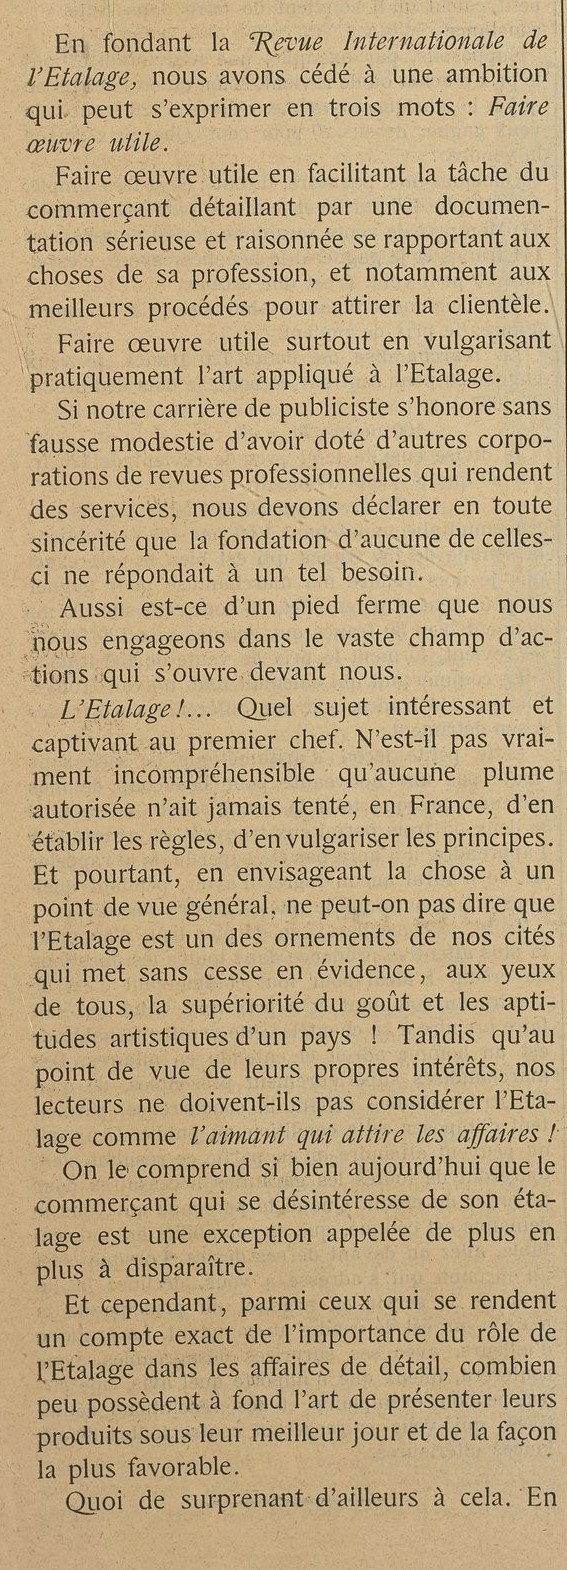
\includegraphics{./images/N1_avril1909b.jpeg}

}

\caption{Lettre de motivation}

\end{figure}%

\url{https://gabriben.github.io/NLP.html\#introduction}

\begin{Shaded}
\begin{Highlighting}[]
\FunctionTok{library}\NormalTok{(tesseract)}
\FunctionTok{tesseract\_download}\NormalTok{(}\StringTok{"fra"}\NormalTok{) }\CommentTok{\#pour télécharger le modèle de langage}
\end{Highlighting}
\end{Shaded}

\begin{verbatim}
[1] "C:\\Users\\33623\\AppData\\Local\\tesseract5\\tesseract5\\tessdata/fra.traineddata"
\end{verbatim}

\begin{Shaded}
\begin{Highlighting}[]
\NormalTok{t1}\OtherTok{\textless{}{-}}\FunctionTok{Sys.time}\NormalTok{()}
\NormalTok{text }\OtherTok{\textless{}{-}}\NormalTok{ tesseract}\SpecialCharTok{::}\FunctionTok{ocr}\NormalTok{(}\StringTok{"./data/N1\_avril1909b.jpeg"}\NormalTok{, }\AttributeTok{engine =} \StringTok{"fra"}\NormalTok{)}
\NormalTok{t2}\OtherTok{\textless{}{-}}\FunctionTok{Sys.time}\NormalTok{()}
\NormalTok{t}\OtherTok{\textless{}{-}}\NormalTok{ t2}\SpecialCharTok{{-}}\NormalTok{t1 }\CommentTok{\#pour compter le temps de calcul}
\FunctionTok{cat}\NormalTok{(text) }\CommentTok{\#pour afficher le texte avec sa mise en page}
\end{Highlighting}
\end{Shaded}

\begin{verbatim}
En fondant la ‘Revue Internationale de
l'Etalage, nous avons cédé à une ambition
qui. peut s'exprimer en trois mots : Faire
œuvre ulile.

Faire œuvre utile en facilitant la tâche du
commerçant détaillant par une documen-
tation sérieuse et raisonnée se rapportant aux
choses de sa profession, et notamment aux
meilleurs procédés pour attirer la clientèle.

Faire œuvre utile surtout en vulgarisant
pratiquement l’art appliqué à l'Etalage.

Si notre carrière de publiciste s'honore sans
fausse modestie d’avoir doté d’autres corpo-
rations de revues professionnelles qui rendent
des services, nous devons déclarer en toute
sincérité que la fondation d'aucune de celles- ;
ci ne répondait à un tel besoin.

Aussi est-ce d’un pied ferme que nous
nous engageons dans le vaste champ d’ac-
tions qui s'ouvre devant nous.

L'Etalage!.. Quel sujet intéressant et
captivant au premier chef. N’est-il pas vrai-
ment incompréhensible qu'aucuñe plume
autorisée n’ait jamais tenté, en France, d'en
établir les règles, d’en vulgariser les principes.
Et pourtant, en envisageant la chose à un
point de vue général, ne peut-on pas dire que
l'Etalage est un des ornements de nos cités
qui met sans cesse en évidence, aux yeux
de tous, la supériorité du goût et les apti-
tudes artistiques d’un pays ! Tandis qu’au
point dé vue de leurs propres intérêts, nos
lecteurs ne doivent-ils pas considérer l’Eta-
lage comme l'aimant qui attire les affaires !

On le comprend si bien aujourd’hui que le
commerçant qui se désintéresse de son éta-
lage est une exception appelée de plus en
plus à disparaître.

Et cependant, parmi ceux qui se rendent
un compte exact de l’importance du rôle de
VEtalage dans les affaires de détail, combien
peu possèdent à fond l’art de présenter leurs
produits sous leur meilleur jour et de la façon
la plus favorable. ‘

Quoi de surprenant d’ailleurs à cela. En
\end{verbatim}

\begin{Shaded}
\begin{Highlighting}[]
\CommentTok{\#tesseract\_info() \#voir les langues disponibles}
\NormalTok{t}
\end{Highlighting}
\end{Shaded}

\begin{verbatim}
Time difference of 1.836614 secs
\end{verbatim}

Pour améliorer la performance qui peut se mesurer au niveau des lettres,
mais doit surtout l'être au niveau des mots, deux stratégies sont
possibles. La première de pre-processing, la seconde de post-processing
avec un mécanisme de détection et de correction d'erreurs. Le
pre-processing consiste à traiter l'image en renforçant les contrastes ,
en éliminant le bruit, on en rend les pixels mieux digestes pour
tesseract. C'est ce à quoi s'attache le package magick qui offre un
bouquet de fonctions à cette fin. Nous laissons le lecteur le tester
seul.

Le post-processing sert à introduire des mécanismes de correction
d'erreurs au niveau des mots. Pour une idée de ce type de développement
voir \href{https://gabriben.github.io/NLP.html}{Gabriel, Yadir, Xiaojie,
Mingyu}

Naturellement, un paramètre important est la vitesse de traitement des
images. Dans un projet complet on peut être amener à traiter des
centaines images en boucle. Dans notre exemple la durée est de
\texttt{t} secondes, autrement dit 6 images à la minute ou 360 à
l'heure\ldots{}

\subsection{Du speech au texte}\label{du-speech-au-texte}

La tradition méthodologique de la sociologie est celle de l'entretien,
avec toute sorte d'acteurs. Elle aboutit à la production de
transcriptions, plus ou moins détaillées et précises. Mais des textes

On peut désormais enregistrer la paroles des interfaces vocales. Le
speech to text est de plus en plus efficace, voir l'API de google. Il
existe déja des packages sur R qui permettent d'accéder aux solutions de
google langage qui nécessite une clé d'API.

\url{https://cran.r-project.org/web/packages/googleLanguageR/vignettes/setup.html}

une autre solution

On ne fait qu'entre-ouvrir le sujet, mais il est certainement un des
futurs du NLP.

\section{L'exploitation de base de données
textuelles}\label{lexploitation-de-base-de-donnuxe9es-textuelles}

Les bases de données textuelles sont désormais nombreuses , variées et
normalisées. Elles permettent de constituer rapidement des corpus
étoffés

\subsection{le cas Europresse}\label{le-cas-europresse}

On commence par un exemple simple en utilisant la base
\href{http://www.europresse.com/fr/}{europresse}. L'objectif est de
constituer un fichier de références bibliographiques, exploitable via R.

Dans Europresse , nous avons fait une recherche sur les articles
comprenant le terme '' vaccination'' dans la presse nationale
françaises, constituées de 14 titres. On retient les 400 derniers
articles du mois de Juillet 2021, le 12 le Président faisait une
allocution.

On utilise
\href{https://revtools.net/data.html\#importing-to-r}{revtools} pour sa
fonction d'importation des fichiers au format .ris et de transformation
en data frame structuré

\begin{Shaded}
\begin{Highlighting}[]
\FunctionTok{library}\NormalTok{(revtools)}
\NormalTok{df }\OtherTok{\textless{}{-}} \FunctionTok{read\_bibliography}\NormalTok{(}\FunctionTok{iconv}\NormalTok{(}\StringTok{"./data/vaccination.ris"}\NormalTok{))}\SpecialCharTok{\%\textgreater{}\%}
  \FunctionTok{mutate}\NormalTok{(}\AttributeTok{jour=}\FunctionTok{str\_sub}\NormalTok{(DA, }\DecValTok{9}\NormalTok{,}\DecValTok{10}\NormalTok{))}

\FunctionTok{flextable}\NormalTok{(}\FunctionTok{head}\NormalTok{(df,}\DecValTok{3}\NormalTok{))}
\end{Highlighting}
\end{Shaded}

\global\setlength{\Oldarrayrulewidth}{\arrayrulewidth}

\global\setlength{\Oldtabcolsep}{\tabcolsep}

\setlength{\tabcolsep}{0pt}

\renewcommand*{\arraystretch}{1.5}



\providecommand{\ascline}[3]{\noalign{\global\arrayrulewidth #1}\arrayrulecolor[HTML]{#2}\cline{#3}}

\begin{longtable*}[c]{|p{0.75in}|p{0.75in}|p{0.75in}|p{0.75in}|p{0.75in}|p{0.75in}|p{0.75in}|p{0.75in}|p{0.75in}|p{0.75in}|p{0.75in}|p{0.75in}|p{0.75in}}



\hhline{>{\arrayrulecolor[HTML]{666666}\global\arrayrulewidth=1.5pt}->{\arrayrulecolor[HTML]{666666}\global\arrayrulewidth=1.5pt}->{\arrayrulecolor[HTML]{666666}\global\arrayrulewidth=1.5pt}->{\arrayrulecolor[HTML]{666666}\global\arrayrulewidth=1.5pt}->{\arrayrulecolor[HTML]{666666}\global\arrayrulewidth=1.5pt}->{\arrayrulecolor[HTML]{666666}\global\arrayrulewidth=1.5pt}->{\arrayrulecolor[HTML]{666666}\global\arrayrulewidth=1.5pt}->{\arrayrulecolor[HTML]{666666}\global\arrayrulewidth=1.5pt}->{\arrayrulecolor[HTML]{666666}\global\arrayrulewidth=1.5pt}->{\arrayrulecolor[HTML]{666666}\global\arrayrulewidth=1.5pt}->{\arrayrulecolor[HTML]{666666}\global\arrayrulewidth=1.5pt}->{\arrayrulecolor[HTML]{666666}\global\arrayrulewidth=1.5pt}->{\arrayrulecolor[HTML]{666666}\global\arrayrulewidth=1.5pt}-}

\multicolumn{1}{>{\cellcolor[HTML]{EFEFEF}\raggedright}m{\dimexpr 0.75in+0\tabcolsep}}{\textcolor[HTML]{000000}{\fontsize{10}{10}\selectfont{\textbf{label}}}} & \multicolumn{1}{>{\cellcolor[HTML]{EFEFEF}\raggedright}m{\dimexpr 0.75in+0\tabcolsep}}{\textcolor[HTML]{000000}{\fontsize{10}{10}\selectfont{\textbf{type}}}} & \multicolumn{1}{>{\cellcolor[HTML]{EFEFEF}\raggedright}m{\dimexpr 0.75in+0\tabcolsep}}{\textcolor[HTML]{000000}{\fontsize{10}{10}\selectfont{\textbf{title}}}} & \multicolumn{1}{>{\cellcolor[HTML]{EFEFEF}\raggedright}m{\dimexpr 0.75in+0\tabcolsep}}{\textcolor[HTML]{000000}{\fontsize{10}{10}\selectfont{\textbf{author}}}} & \multicolumn{1}{>{\cellcolor[HTML]{EFEFEF}\raggedright}m{\dimexpr 0.75in+0\tabcolsep}}{\textcolor[HTML]{000000}{\fontsize{10}{10}\selectfont{\textbf{journal}}}} & \multicolumn{1}{>{\cellcolor[HTML]{EFEFEF}\raggedright}m{\dimexpr 0.75in+0\tabcolsep}}{\textcolor[HTML]{000000}{\fontsize{10}{10}\selectfont{\textbf{abstract}}}} & \multicolumn{1}{>{\cellcolor[HTML]{EFEFEF}\raggedright}m{\dimexpr 0.75in+0\tabcolsep}}{\textcolor[HTML]{000000}{\fontsize{10}{10}\selectfont{\textbf{institution}}}} & \multicolumn{1}{>{\cellcolor[HTML]{EFEFEF}\raggedright}m{\dimexpr 0.75in+0\tabcolsep}}{\textcolor[HTML]{000000}{\fontsize{10}{10}\selectfont{\textbf{year}}}} & \multicolumn{1}{>{\cellcolor[HTML]{EFEFEF}\raggedright}m{\dimexpr 0.75in+0\tabcolsep}}{\textcolor[HTML]{000000}{\fontsize{10}{10}\selectfont{\textbf{pages}}}} & \multicolumn{1}{>{\cellcolor[HTML]{EFEFEF}\raggedright}m{\dimexpr 0.75in+0\tabcolsep}}{\textcolor[HTML]{000000}{\fontsize{10}{10}\selectfont{\textbf{language}}}} & \multicolumn{1}{>{\cellcolor[HTML]{EFEFEF}\raggedright}m{\dimexpr 0.75in+0\tabcolsep}}{\textcolor[HTML]{000000}{\fontsize{10}{10}\selectfont{\textbf{url}}}} & \multicolumn{1}{>{\cellcolor[HTML]{EFEFEF}\raggedright}m{\dimexpr 0.75in+0\tabcolsep}}{\textcolor[HTML]{000000}{\fontsize{10}{10}\selectfont{\textbf{DA}}}} & \multicolumn{1}{>{\cellcolor[HTML]{EFEFEF}\raggedright}m{\dimexpr 0.75in+0\tabcolsep}}{\textcolor[HTML]{000000}{\fontsize{10}{10}\selectfont{\textbf{jour}}}} \\

\noalign{\global\arrayrulewidth 0pt}\arrayrulecolor[HTML]{000000}

\hhline{>{\arrayrulecolor[HTML]{666666}\global\arrayrulewidth=1.5pt}->{\arrayrulecolor[HTML]{666666}\global\arrayrulewidth=1.5pt}->{\arrayrulecolor[HTML]{666666}\global\arrayrulewidth=1.5pt}->{\arrayrulecolor[HTML]{666666}\global\arrayrulewidth=1.5pt}->{\arrayrulecolor[HTML]{666666}\global\arrayrulewidth=1.5pt}->{\arrayrulecolor[HTML]{666666}\global\arrayrulewidth=1.5pt}->{\arrayrulecolor[HTML]{666666}\global\arrayrulewidth=1.5pt}->{\arrayrulecolor[HTML]{666666}\global\arrayrulewidth=1.5pt}->{\arrayrulecolor[HTML]{666666}\global\arrayrulewidth=1.5pt}->{\arrayrulecolor[HTML]{666666}\global\arrayrulewidth=1.5pt}->{\arrayrulecolor[HTML]{666666}\global\arrayrulewidth=1.5pt}->{\arrayrulecolor[HTML]{666666}\global\arrayrulewidth=1.5pt}->{\arrayrulecolor[HTML]{666666}\global\arrayrulewidth=1.5pt}-}\endfirsthead 

\hhline{>{\arrayrulecolor[HTML]{666666}\global\arrayrulewidth=1.5pt}->{\arrayrulecolor[HTML]{666666}\global\arrayrulewidth=1.5pt}->{\arrayrulecolor[HTML]{666666}\global\arrayrulewidth=1.5pt}->{\arrayrulecolor[HTML]{666666}\global\arrayrulewidth=1.5pt}->{\arrayrulecolor[HTML]{666666}\global\arrayrulewidth=1.5pt}->{\arrayrulecolor[HTML]{666666}\global\arrayrulewidth=1.5pt}->{\arrayrulecolor[HTML]{666666}\global\arrayrulewidth=1.5pt}->{\arrayrulecolor[HTML]{666666}\global\arrayrulewidth=1.5pt}->{\arrayrulecolor[HTML]{666666}\global\arrayrulewidth=1.5pt}->{\arrayrulecolor[HTML]{666666}\global\arrayrulewidth=1.5pt}->{\arrayrulecolor[HTML]{666666}\global\arrayrulewidth=1.5pt}->{\arrayrulecolor[HTML]{666666}\global\arrayrulewidth=1.5pt}->{\arrayrulecolor[HTML]{666666}\global\arrayrulewidth=1.5pt}-}

\multicolumn{1}{>{\cellcolor[HTML]{EFEFEF}\raggedright}m{\dimexpr 0.75in+0\tabcolsep}}{\textcolor[HTML]{000000}{\fontsize{10}{10}\selectfont{\textbf{label}}}} & \multicolumn{1}{>{\cellcolor[HTML]{EFEFEF}\raggedright}m{\dimexpr 0.75in+0\tabcolsep}}{\textcolor[HTML]{000000}{\fontsize{10}{10}\selectfont{\textbf{type}}}} & \multicolumn{1}{>{\cellcolor[HTML]{EFEFEF}\raggedright}m{\dimexpr 0.75in+0\tabcolsep}}{\textcolor[HTML]{000000}{\fontsize{10}{10}\selectfont{\textbf{title}}}} & \multicolumn{1}{>{\cellcolor[HTML]{EFEFEF}\raggedright}m{\dimexpr 0.75in+0\tabcolsep}}{\textcolor[HTML]{000000}{\fontsize{10}{10}\selectfont{\textbf{author}}}} & \multicolumn{1}{>{\cellcolor[HTML]{EFEFEF}\raggedright}m{\dimexpr 0.75in+0\tabcolsep}}{\textcolor[HTML]{000000}{\fontsize{10}{10}\selectfont{\textbf{journal}}}} & \multicolumn{1}{>{\cellcolor[HTML]{EFEFEF}\raggedright}m{\dimexpr 0.75in+0\tabcolsep}}{\textcolor[HTML]{000000}{\fontsize{10}{10}\selectfont{\textbf{abstract}}}} & \multicolumn{1}{>{\cellcolor[HTML]{EFEFEF}\raggedright}m{\dimexpr 0.75in+0\tabcolsep}}{\textcolor[HTML]{000000}{\fontsize{10}{10}\selectfont{\textbf{institution}}}} & \multicolumn{1}{>{\cellcolor[HTML]{EFEFEF}\raggedright}m{\dimexpr 0.75in+0\tabcolsep}}{\textcolor[HTML]{000000}{\fontsize{10}{10}\selectfont{\textbf{year}}}} & \multicolumn{1}{>{\cellcolor[HTML]{EFEFEF}\raggedright}m{\dimexpr 0.75in+0\tabcolsep}}{\textcolor[HTML]{000000}{\fontsize{10}{10}\selectfont{\textbf{pages}}}} & \multicolumn{1}{>{\cellcolor[HTML]{EFEFEF}\raggedright}m{\dimexpr 0.75in+0\tabcolsep}}{\textcolor[HTML]{000000}{\fontsize{10}{10}\selectfont{\textbf{language}}}} & \multicolumn{1}{>{\cellcolor[HTML]{EFEFEF}\raggedright}m{\dimexpr 0.75in+0\tabcolsep}}{\textcolor[HTML]{000000}{\fontsize{10}{10}\selectfont{\textbf{url}}}} & \multicolumn{1}{>{\cellcolor[HTML]{EFEFEF}\raggedright}m{\dimexpr 0.75in+0\tabcolsep}}{\textcolor[HTML]{000000}{\fontsize{10}{10}\selectfont{\textbf{DA}}}} & \multicolumn{1}{>{\cellcolor[HTML]{EFEFEF}\raggedright}m{\dimexpr 0.75in+0\tabcolsep}}{\textcolor[HTML]{000000}{\fontsize{10}{10}\selectfont{\textbf{jour}}}} \\

\noalign{\global\arrayrulewidth 0pt}\arrayrulecolor[HTML]{000000}

\hhline{>{\arrayrulecolor[HTML]{666666}\global\arrayrulewidth=1.5pt}->{\arrayrulecolor[HTML]{666666}\global\arrayrulewidth=1.5pt}->{\arrayrulecolor[HTML]{666666}\global\arrayrulewidth=1.5pt}->{\arrayrulecolor[HTML]{666666}\global\arrayrulewidth=1.5pt}->{\arrayrulecolor[HTML]{666666}\global\arrayrulewidth=1.5pt}->{\arrayrulecolor[HTML]{666666}\global\arrayrulewidth=1.5pt}->{\arrayrulecolor[HTML]{666666}\global\arrayrulewidth=1.5pt}->{\arrayrulecolor[HTML]{666666}\global\arrayrulewidth=1.5pt}->{\arrayrulecolor[HTML]{666666}\global\arrayrulewidth=1.5pt}->{\arrayrulecolor[HTML]{666666}\global\arrayrulewidth=1.5pt}->{\arrayrulecolor[HTML]{666666}\global\arrayrulewidth=1.5pt}->{\arrayrulecolor[HTML]{666666}\global\arrayrulewidth=1.5pt}->{\arrayrulecolor[HTML]{666666}\global\arrayrulewidth=1.5pt}-}\endhead



\multicolumn{1}{>{\cellcolor[HTML]{EFEFEF}\raggedright}m{\dimexpr 0.75in+0\tabcolsep}}{\textcolor[HTML]{000000}{\fontsize{10}{10}\selectfont{Paul.Ortoli\_2021\_LeMo}}} & \multicolumn{1}{>{\cellcolor[HTML]{EFEFEF}\raggedright}m{\dimexpr 0.75in+0\tabcolsep}}{\textcolor[HTML]{000000}{\fontsize{10}{10}\selectfont{NEWS}}} & \multicolumn{1}{>{\cellcolor[HTML]{EFEFEF}\raggedright}m{\dimexpr 0.75in+0\tabcolsep}}{\textcolor[HTML]{000000}{\fontsize{10}{10}\selectfont{La\ Corse\ redoute\ une\ généralisation\ de\ la\ reprise\ épidémique}}} & \multicolumn{1}{>{\cellcolor[HTML]{EFEFEF}\raggedright}m{\dimexpr 0.75in+0\tabcolsep}}{\textcolor[HTML]{000000}{\fontsize{10}{10}\selectfont{Paul\ Ortoli}}} & \multicolumn{1}{>{\cellcolor[HTML]{EFEFEF}\raggedright}m{\dimexpr 0.75in+0\tabcolsep}}{\textcolor[HTML]{000000}{\fontsize{10}{10}\selectfont{Le\ Monde}}} & \multicolumn{1}{>{\cellcolor[HTML]{EFEFEF}\raggedright}m{\dimexpr 0.75in+0\tabcolsep}}{\textcolor[HTML]{000000}{\fontsize{10}{10}\selectfont{Alors\ que\ la\ Balagne,\ en\ Haute-Corse,\ a\ atteint\ vendredi\ 16\ juillet\ un\ taux\ d'incidence\ de\ 1\ 066\ cas\ pour\ 100\ 000\ habitants,\ et\ un\ taux\ de\ positivit<c3><a9>\ de\ 10\ ...}}} & \multicolumn{1}{>{\cellcolor[HTML]{EFEFEF}\raggedright}m{\dimexpr 0.75in+0\tabcolsep}}{\textcolor[HTML]{000000}{\fontsize{10}{10}\selectfont{Ajaccio\ correspondant}}} & \multicolumn{1}{>{\cellcolor[HTML]{EFEFEF}\raggedright}m{\dimexpr 0.75in+0\tabcolsep}}{\textcolor[HTML]{000000}{\fontsize{10}{10}\selectfont{2021}}} & \multicolumn{1}{>{\cellcolor[HTML]{EFEFEF}\raggedright}m{\dimexpr 0.75in+0\tabcolsep}}{\textcolor[HTML]{000000}{\fontsize{10}{10}\selectfont{9}}} & \multicolumn{1}{>{\cellcolor[HTML]{EFEFEF}\raggedright}m{\dimexpr 0.75in+0\tabcolsep}}{\textcolor[HTML]{000000}{\fontsize{10}{10}\selectfont{Français}}} & \multicolumn{1}{>{\cellcolor[HTML]{EFEFEF}\raggedright}m{\dimexpr 0.75in+0\tabcolsep}}{\textcolor[HTML]{000000}{\fontsize{10}{10}\selectfont{https://nouveau.europresse.com/Link/PARIS10T\_1/news\%c2\%b720210720\%c2\%b7LM\%c2\%b74416628}}} & \multicolumn{1}{>{\cellcolor[HTML]{EFEFEF}\raggedright}m{\dimexpr 0.75in+0\tabcolsep}}{\textcolor[HTML]{000000}{\fontsize{10}{10}\selectfont{2021/07/20/}}} & \multicolumn{1}{>{\cellcolor[HTML]{EFEFEF}\raggedright}m{\dimexpr 0.75in+0\tabcolsep}}{\textcolor[HTML]{000000}{\fontsize{10}{10}\selectfont{20}}} \\

\noalign{\global\arrayrulewidth 0pt}\arrayrulecolor[HTML]{000000}

\hhline{>{\arrayrulecolor[HTML]{666666}\global\arrayrulewidth=0.75pt}->{\arrayrulecolor[HTML]{666666}\global\arrayrulewidth=0.75pt}->{\arrayrulecolor[HTML]{666666}\global\arrayrulewidth=0.75pt}->{\arrayrulecolor[HTML]{666666}\global\arrayrulewidth=0.75pt}->{\arrayrulecolor[HTML]{666666}\global\arrayrulewidth=0.75pt}->{\arrayrulecolor[HTML]{666666}\global\arrayrulewidth=0.75pt}->{\arrayrulecolor[HTML]{666666}\global\arrayrulewidth=0.75pt}->{\arrayrulecolor[HTML]{666666}\global\arrayrulewidth=0.75pt}->{\arrayrulecolor[HTML]{666666}\global\arrayrulewidth=0.75pt}->{\arrayrulecolor[HTML]{666666}\global\arrayrulewidth=0.75pt}->{\arrayrulecolor[HTML]{666666}\global\arrayrulewidth=0.75pt}->{\arrayrulecolor[HTML]{666666}\global\arrayrulewidth=0.75pt}->{\arrayrulecolor[HTML]{666666}\global\arrayrulewidth=0.75pt}-}



\multicolumn{1}{>{\cellcolor[HTML]{EFEFEF}\raggedright}m{\dimexpr 0.75in+0\tabcolsep}}{\textcolor[HTML]{000000}{\fontsize{10}{10}\selectfont{X2021\_LeMo}}} & \multicolumn{1}{>{\cellcolor[HTML]{EFEFEF}\raggedright}m{\dimexpr 0.75in+0\tabcolsep}}{\textcolor[HTML]{000000}{\fontsize{10}{10}\selectfont{NEWS}}} & \multicolumn{1}{>{\cellcolor[HTML]{EFEFEF}\raggedright}m{\dimexpr 0.75in+0\tabcolsep}}{\textcolor[HTML]{000000}{\fontsize{10}{10}\selectfont{Enquête\ ouverte\ après\ l'incendie\ d'un\ centre\ de\ vaccination}}} & \multicolumn{1}{>{\cellcolor[HTML]{EFEFEF}\raggedright}m{\dimexpr 0.75in+0\tabcolsep}}{\textcolor[HTML]{000000}{\fontsize{10}{10}\selectfont{}}} & \multicolumn{1}{>{\cellcolor[HTML]{EFEFEF}\raggedright}m{\dimexpr 0.75in+0\tabcolsep}}{\textcolor[HTML]{000000}{\fontsize{10}{10}\selectfont{Le\ Monde}}} & \multicolumn{1}{>{\cellcolor[HTML]{EFEFEF}\raggedright}m{\dimexpr 0.75in+0\tabcolsep}}{\textcolor[HTML]{000000}{\fontsize{10}{10}\selectfont{Le\ centre\ de\ vaccination\ contre\ le\ Covid-19\ de\ la\ commune\ d'Urrugne,\ dans\ les\ Pyr<c3><a9>n<c3><a9>es-Atlantiques,\ d<c3><a9>partement\ o<c3><b9>\ le\ taux\ d'incidence\ est\ sup<c3><a9>rieur\ au\ seuil\ d'alerte,\ a\ <c3><a9>t<c3><a9>\ ...}}} & \multicolumn{1}{>{\cellcolor[HTML]{EFEFEF}\raggedright}m{\dimexpr 0.75in+0\tabcolsep}}{\textcolor[HTML]{000000}{\fontsize{10}{10}\selectfont{}}} & \multicolumn{1}{>{\cellcolor[HTML]{EFEFEF}\raggedright}m{\dimexpr 0.75in+0\tabcolsep}}{\textcolor[HTML]{000000}{\fontsize{10}{10}\selectfont{2021}}} & \multicolumn{1}{>{\cellcolor[HTML]{EFEFEF}\raggedright}m{\dimexpr 0.75in+0\tabcolsep}}{\textcolor[HTML]{000000}{\fontsize{10}{10}\selectfont{12}}} & \multicolumn{1}{>{\cellcolor[HTML]{EFEFEF}\raggedright}m{\dimexpr 0.75in+0\tabcolsep}}{\textcolor[HTML]{000000}{\fontsize{10}{10}\selectfont{Français}}} & \multicolumn{1}{>{\cellcolor[HTML]{EFEFEF}\raggedright}m{\dimexpr 0.75in+0\tabcolsep}}{\textcolor[HTML]{000000}{\fontsize{10}{10}\selectfont{https://nouveau.europresse.com/Link/PARIS10T\_1/news\%c2\%b720210720\%c2\%b7LM\%c2\%b75516067}}} & \multicolumn{1}{>{\cellcolor[HTML]{EFEFEF}\raggedright}m{\dimexpr 0.75in+0\tabcolsep}}{\textcolor[HTML]{000000}{\fontsize{10}{10}\selectfont{2021/07/20/}}} & \multicolumn{1}{>{\cellcolor[HTML]{EFEFEF}\raggedright}m{\dimexpr 0.75in+0\tabcolsep}}{\textcolor[HTML]{000000}{\fontsize{10}{10}\selectfont{20}}} \\

\noalign{\global\arrayrulewidth 0pt}\arrayrulecolor[HTML]{000000}

\hhline{>{\arrayrulecolor[HTML]{666666}\global\arrayrulewidth=0.75pt}->{\arrayrulecolor[HTML]{666666}\global\arrayrulewidth=0.75pt}->{\arrayrulecolor[HTML]{666666}\global\arrayrulewidth=0.75pt}->{\arrayrulecolor[HTML]{666666}\global\arrayrulewidth=0.75pt}->{\arrayrulecolor[HTML]{666666}\global\arrayrulewidth=0.75pt}->{\arrayrulecolor[HTML]{666666}\global\arrayrulewidth=0.75pt}->{\arrayrulecolor[HTML]{666666}\global\arrayrulewidth=0.75pt}->{\arrayrulecolor[HTML]{666666}\global\arrayrulewidth=0.75pt}->{\arrayrulecolor[HTML]{666666}\global\arrayrulewidth=0.75pt}->{\arrayrulecolor[HTML]{666666}\global\arrayrulewidth=0.75pt}->{\arrayrulecolor[HTML]{666666}\global\arrayrulewidth=0.75pt}->{\arrayrulecolor[HTML]{666666}\global\arrayrulewidth=0.75pt}->{\arrayrulecolor[HTML]{666666}\global\arrayrulewidth=0.75pt}-}



\multicolumn{1}{>{\cellcolor[HTML]{EFEFEF}\raggedright}m{\dimexpr 0.75in+0\tabcolsep}}{\textcolor[HTML]{000000}{\fontsize{10}{10}\selectfont{Catherine.Pacary\_2021\_LeMo}}} & \multicolumn{1}{>{\cellcolor[HTML]{EFEFEF}\raggedright}m{\dimexpr 0.75in+0\tabcolsep}}{\textcolor[HTML]{000000}{\fontsize{10}{10}\selectfont{NEWS}}} & \multicolumn{1}{>{\cellcolor[HTML]{EFEFEF}\raggedright}m{\dimexpr 0.75in+0\tabcolsep}}{\textcolor[HTML]{000000}{\fontsize{10}{10}\selectfont{Enquête\ sur\ le\ record\ de\ vitesse\ des\ vaccins\ contre\ le\ Covid-19}}} & \multicolumn{1}{>{\cellcolor[HTML]{EFEFEF}\raggedright}m{\dimexpr 0.75in+0\tabcolsep}}{\textcolor[HTML]{000000}{\fontsize{10}{10}\selectfont{Catherine\ Pacary}}} & \multicolumn{1}{>{\cellcolor[HTML]{EFEFEF}\raggedright}m{\dimexpr 0.75in+0\tabcolsep}}{\textcolor[HTML]{000000}{\fontsize{10}{10}\selectfont{Le\ Monde}}} & \multicolumn{1}{>{\cellcolor[HTML]{EFEFEF}\raggedright}m{\dimexpr 0.75in+0\tabcolsep}}{\textcolor[HTML]{000000}{\fontsize{10}{10}\selectfont{C'est\ un\ film\ qui\ tombe\ <c3><a0>\ point.\ Alors\ que\ la\ vaccination\ se\ r<c3><a9>v<c3><a8>le\ indispensable\ pour\ lutter\ contre\ la\ pand<c3><a9>mie\ de\ Covid-19,\ il\ r<c3><a9>pond\ <c3><a0>\ une\ interrogation\ r<c3><a9>pandue\ :\ comment\ les\ ...}}} & \multicolumn{1}{>{\cellcolor[HTML]{EFEFEF}\raggedright}m{\dimexpr 0.75in+0\tabcolsep}}{\textcolor[HTML]{000000}{\fontsize{10}{10}\selectfont{Documentaire}}} & \multicolumn{1}{>{\cellcolor[HTML]{EFEFEF}\raggedright}m{\dimexpr 0.75in+0\tabcolsep}}{\textcolor[HTML]{000000}{\fontsize{10}{10}\selectfont{2021}}} & \multicolumn{1}{>{\cellcolor[HTML]{EFEFEF}\raggedright}m{\dimexpr 0.75in+0\tabcolsep}}{\textcolor[HTML]{000000}{\fontsize{10}{10}\selectfont{TEL21}}} & \multicolumn{1}{>{\cellcolor[HTML]{EFEFEF}\raggedright}m{\dimexpr 0.75in+0\tabcolsep}}{\textcolor[HTML]{000000}{\fontsize{10}{10}\selectfont{Français}}} & \multicolumn{1}{>{\cellcolor[HTML]{EFEFEF}\raggedright}m{\dimexpr 0.75in+0\tabcolsep}}{\textcolor[HTML]{000000}{\fontsize{10}{10}\selectfont{https://nouveau.europresse.com/Link/PARIS10T\_1/news\%c2\%b720210720\%c2\%b7LM\%c2\%b70377892}}} & \multicolumn{1}{>{\cellcolor[HTML]{EFEFEF}\raggedright}m{\dimexpr 0.75in+0\tabcolsep}}{\textcolor[HTML]{000000}{\fontsize{10}{10}\selectfont{2021/07/20/}}} & \multicolumn{1}{>{\cellcolor[HTML]{EFEFEF}\raggedright}m{\dimexpr 0.75in+0\tabcolsep}}{\textcolor[HTML]{000000}{\fontsize{10}{10}\selectfont{20}}} \\

\noalign{\global\arrayrulewidth 0pt}\arrayrulecolor[HTML]{000000}

\hhline{>{\arrayrulecolor[HTML]{666666}\global\arrayrulewidth=1.5pt}->{\arrayrulecolor[HTML]{666666}\global\arrayrulewidth=1.5pt}->{\arrayrulecolor[HTML]{666666}\global\arrayrulewidth=1.5pt}->{\arrayrulecolor[HTML]{666666}\global\arrayrulewidth=1.5pt}->{\arrayrulecolor[HTML]{666666}\global\arrayrulewidth=1.5pt}->{\arrayrulecolor[HTML]{666666}\global\arrayrulewidth=1.5pt}->{\arrayrulecolor[HTML]{666666}\global\arrayrulewidth=1.5pt}->{\arrayrulecolor[HTML]{666666}\global\arrayrulewidth=1.5pt}->{\arrayrulecolor[HTML]{666666}\global\arrayrulewidth=1.5pt}->{\arrayrulecolor[HTML]{666666}\global\arrayrulewidth=1.5pt}->{\arrayrulecolor[HTML]{666666}\global\arrayrulewidth=1.5pt}->{\arrayrulecolor[HTML]{666666}\global\arrayrulewidth=1.5pt}->{\arrayrulecolor[HTML]{666666}\global\arrayrulewidth=1.5pt}-}



\end{longtable*}



\arrayrulecolor[HTML]{000000}

\global\setlength{\arrayrulewidth}{\Oldarrayrulewidth}

\global\setlength{\tabcolsep}{\Oldtabcolsep}

\renewcommand*{\arraystretch}{1}

\begin{Shaded}
\begin{Highlighting}[]
\NormalTok{g22}\OtherTok{\textless{}{-}}\FunctionTok{ggplot}\NormalTok{(df, }\FunctionTok{aes}\NormalTok{(}\AttributeTok{x=}\NormalTok{jour))}\SpecialCharTok{+}
  \FunctionTok{geom\_bar}\NormalTok{()}\SpecialCharTok{+}
  \FunctionTok{labs}\NormalTok{(}\AttributeTok{x=} \StringTok{"Jour du mois de Juillet 2021"}\NormalTok{,}\AttributeTok{y=}\ConstantTok{NULL}\NormalTok{)}\SpecialCharTok{+}
  \FunctionTok{geom\_vline}\NormalTok{(}\AttributeTok{xintercept=}\DecValTok{6}\NormalTok{, }\AttributeTok{linetype=}\StringTok{"dashed"}\NormalTok{, }\AttributeTok{color =} \StringTok{"red"}\NormalTok{)}\SpecialCharTok{+}
  \FunctionTok{facet\_grid}\NormalTok{(}\FunctionTok{vars}\NormalTok{(journal))}
\NormalTok{g22}
\end{Highlighting}
\end{Shaded}

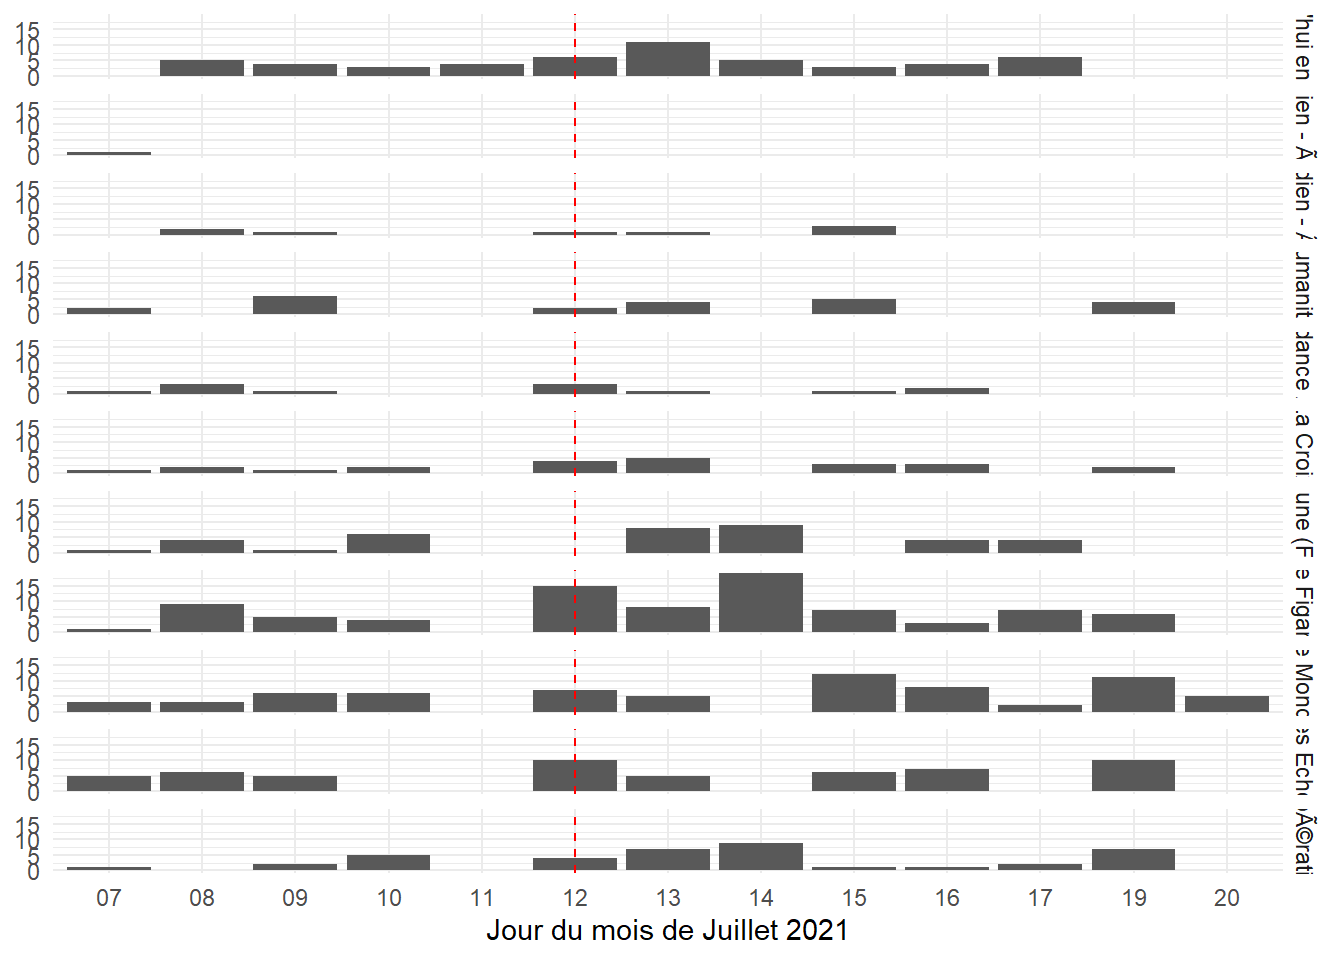
\includegraphics{q03_corpus_suite_files/figure-pdf/unnamed-chunk-1-1.pdf}

\subsection{Jouer avec les bases
bibliographiques}\label{jouer-avec-les-bases-bibliographiques}

\texttt{Fulltext} doit être développé.

\url{https://books.ropensci.org/fulltext/data-sources.html}

On propose un cas à partir de scopus ( demander à Olivier)

\section{Lire le web : Scrapping}\label{lire-le-web-scrapping}

Le scrapping correspond à un internet sauvage où la collecte
d'informations se traduit par une technique de chasseurs-cueilleurs, le
glanage. C'est l'activité qui consiste à moissonner les informations
disponibles sur le net en simulant et en automatisant la lecture par un
navigateur (on préfère l'expression des québécois : des butineurs).

Elle consiste à construire un robot capable de lire et d'enregistrer les
informations disponibles sous forme html puis à les distribuer (parsing)
dans des tableaux structurés, selon une stratégie d'exploration du web
préalablement définie. En réalité le scrapping pose deux problèmes :

\begin{itemize}
\item
  Celui de la structure de recherche. C'est le problème que relève les
  spiders, des robots qui recherchent dans les pages des liens, et vont
  de proche en proche, de lien en lien, pour explorer un domaine. Ils
  peuvent être plus systématiques et prendre davantage de l'organisation
  et structure d'un site web pour énumérer les pages.
\item
  Celui de la collecte de l'information sur chacune des pages. Il
  s'appuie sur le principe que le langage html est un langage à balise
  où le contenu et le contenant sont clairement séparés. Par exemple,
  dans le corps de texte d'une page on définira un titre par la balise

  dont l'instruction s'achève par la balise

  . On sépare ainsi clairement le contenu de la forme.
\end{itemize}

`

Un titre de niveau 1 (un gros titre)

\begin{verbatim}
<p>Un paragraphe.</p>

<h2>Un titre de niveau 2 (un sous titre)</h2>
  <p>Un paragraphe.</p>

  <h3>Un titre de niveau 3 (un sous-sous titre)</h3>
    <p>Etc.</p>
\end{verbatim}

`

Ultérieurement on pourra définir les propriétés graphiques d'une balise
par des CSS. Par exemple avec ceci, les paragraphes seront publiés en
caractère bleu.

\texttt{p\{\ \ \ \ \ color:\ blue;\ \}}

Ce qui nous intéresse n'est pas la décoration, mais le fait que les
développeurs définissent des balises spécifiques pour chacun des
éléments de leurs pages web, et que si nous savons les repérer , nous
avons le moyen de mieux lire le texte. Les balises sont la cible du
scrapping. Ces dernières peuvent néanmoins être protégées par les
développeurs et encapsulées par d'autres langages informatique rendant
leur butinage impossible. L'information n'est alors plus contenue dans
la balise et le code source d'une page web.

De nombreuses ressources sont disponibles, mais pour en rester à R , le
package rvest permet de réaliser des extractions simples mais
suffisantes pour de nombreux usages.

Une application rvest :

\url{https://www.r-bloggers.com/2018/10/first-release-and-update-dates-of-r-packages-statistics/}

Le package rvest est générique :

\url{https://community.rstudio.com/t/scraping-messages-in-forum-using-rvest/27846/2}

Voici un petit exemple sur du contenu d'un forum de VTC, un thread
relatif à la question de la vaccination obligatoire.

\begin{Shaded}
\begin{Highlighting}[]
\FunctionTok{library}\NormalTok{(rvest)}

\CommentTok{\# Scrape thread titles, thread links, authors and number of views}

\NormalTok{start }\OtherTok{\textless{}{-}} \StringTok{"https://uberzone.fr/threads/si{-}la{-}vaccination{-}devient{-}obligatoire{-}vous{-}feriez{-}vous{-}vacciner{-}ou{-}changeriez{-}vous{-}de{-}corps{-}de{-}metier.17425"}

\NormalTok{x}\OtherTok{\textless{}{-}}\FunctionTok{c}\NormalTok{(}\StringTok{"/page{-}2"}\NormalTok{, }\StringTok{"/page{-}3"}\NormalTok{, }\StringTok{"/page{-}4"}\NormalTok{)}

\ControlFlowTok{for}\NormalTok{ (val }\ControlFlowTok{in}\NormalTok{ x)\{}
\NormalTok{  url}\OtherTok{\textless{}{-}}\FunctionTok{paste0}\NormalTok{(start,val)}
\NormalTok{  h }\OtherTok{\textless{}{-}} \FunctionTok{read\_html}\NormalTok{(url)}

\NormalTok{post }\OtherTok{\textless{}{-}}\NormalTok{ h }\SpecialCharTok{\%\textgreater{}\%}
  \FunctionTok{html\_nodes}\NormalTok{(}\StringTok{".bbWrapper"}\NormalTok{) }\SpecialCharTok{\%\textgreater{}\%}
  \FunctionTok{html\_text}\NormalTok{()}\SpecialCharTok{\%\textgreater{}\%}
      \FunctionTok{str\_replace\_all}\NormalTok{(}\AttributeTok{pattern =} \StringTok{"}\SpecialCharTok{\textbackslash{}t}\StringTok{|}\SpecialCharTok{\textbackslash{}r}\StringTok{|}\SpecialCharTok{\textbackslash{}n}\StringTok{"}\NormalTok{, }\AttributeTok{replacement =} \StringTok{""}\NormalTok{)}
\NormalTok{post}
\CommentTok{\#authors \textless{}{-} h \%\textgreater{}\%}
\CommentTok{\#  html\_nodes(".username{-}{-}style2 ") \%\textgreater{}\%}
\CommentTok{\#  html\_text() \%\textgreater{}\%}
\CommentTok{\#  str\_replace\_all(pattern = "\textbackslash{}t|\textbackslash{}r|\textbackslash{}n", replacement = "")}

\CommentTok{\# Create master dataset (and scrape messages in each thread in process)}

\NormalTok{master\_data }\OtherTok{\textless{}{-}} 
  \FunctionTok{tibble}\NormalTok{(post)}
\NormalTok{rds\_name}\OtherTok{\textless{}{-}}\FunctionTok{paste0}\NormalTok{(}\StringTok{"./data/df\_"}\NormalTok{,}\FunctionTok{substr}\NormalTok{(val,}\DecValTok{2}\NormalTok{,}\DecValTok{6}\NormalTok{),}\StringTok{".rds"}\NormalTok{)}
\FunctionTok{saveRDS}\NormalTok{(master\_data,rds\_name)}
\NormalTok{\}}

\FunctionTok{head}\NormalTok{(master\_data)}
\end{Highlighting}
\end{Shaded}

\begin{verbatim}
# A tibble: 6 x 1
  post                                                                          
  <chr>                                                                         
1 "Je comprends pas pourquoi persistez-vous à vouloir convaincre alors que vous~
2 "Shibani a dit:Je comprends pas pourquoi persistez-vous à vouloir convaincre ~
3 "*****\"Celui qui ne pète pas et ne rote pas explose\"*****"                  
4 "mez a dit:Ta cirrhose et ton  Cancer du poumon (je te les souhaite pas faut ~
5 "Shibani a dit:Et puis sache que comme je l’ai déjà dit tu peux acheter ton p~
6 "*****\"Celui qui ne pète pas et ne rote pas explose\"*****"                  
\end{verbatim}

\subsection{Des problèmes pratiques, juridiques et
éthiques}\label{des-probluxe8mes-pratiques-juridiques-et-uxe9thiques}

La pratique du scrapping se heurte d'abord à une question technique. Ce
n'est pas un excercice facile, et il doit être confier à des
spécialistes. Il se heurte aussi à différents problèmes d'ordre éthique
et juridique. Si la pratique n'est pas interdite en tant que telle, elle
se confronte à différents droits et principes éthiques

En termes pratiques, le scrapping crée des risques pour les sites :

\begin{itemize}
\tightlist
\item
  Le risque de deny of service, c'est à dire de saturer ou de parasiter
  un système et de s'exposer à ses contre-mesures, comme par exemple,
  des protections.
\item
  Il contribue à la complexification du web, et implique une
  consommation excessive de ressources énergétiques.
\end{itemize}

Et des risques pour la qualité du recueil de données

\begin{itemize}
\tightlist
\item
  Le risque d'information parcellaires, tronquées, inexactes qui
  résultent de ces contre-mesures. Les producteurs développent des
  stratégies moins naives. L'exemple des pages numérotée par ordre de
  production auxquels on substitue un nombre au hasard pour annihilier
  l'information temporelle.
\item
  Le risque matériel de mal lire les informations, pour des raisons
  d'encodage approximatifs.
\end{itemize}

En termes de droits même les conditions légales relèvent de différents
droits :

\begin{itemize}
\tightlist
\item
  De la propriété intellectuelle,
\item
  Du respect de la vie privée,
\item
  Du droit de la concurrence qui sans l'interdire, condamne la copie
  laissant espérer qu'une transformation des données fasse qu'il y
  échappe.
\end{itemize}

Cependant des facilités et tolérances sont souvent accordées quand c'est
dans un objectif de recherche et que des précautions minimales
d'anonymisation ou de pseudonymisation sont prises, que les règles de
conservation et de destruction des données sont précisées.

En termes éthiques

\begin{itemize}
\tightlist
\item
  Un principe éthique essentiel dans la recherche, et ailleurs, et de ne
  pas nuire à la société dans son ensemble, hors cette technique
  participe à la ``robotisation'' du web (plus de 50\% du trafic
  résulterait de la circulation des spiders , scrapers, sniffers et
  autres bots, comme dans la forêt une éthique écologique revient à
  préveler le minimal nécessaire pour l'étude entreprise
\end{itemize}

\section{L'importance croissante des
API}\label{limportance-croissante-des-api}

Les API doivent être considérées comme la voie normale d'accès à
l'information, du moins en droit. Elles relèvent du contrat. Le recours
aux APIs est civilisé, ne serait-ce parce qu'on introduit une sorte
d'étiquette, des règles de courtoisie, un système de reconnaissance
réciproque et d'attribution de droits.

Sur le plan méthodologique elles présentent l'avantage de donner aux
requêtes un caractère reproductible , mêmes si les bases visées peuvent
varier. Elles asurent une grande fiabilité des données.

L'utilisation d'API lève l'ambiguïté légale qui accompagne le scraping
et peut ainsi paraître comme plus ``civilisée''. Elle nécessite
naturellement que le gestionnaire de la base de données fournisse les
moyens de s'identifier et de requêter, elle peut avoir l'inconvénient
d'être coûteuse quand l'accès est payant, ce qui sera de plus en plus le
cas.

\subsection{Un tour d'horizon}\label{un-tour-dhorizon}

La plus part des grandes plateformes offrent des API plus ou moins
ouvertes, examinons-en quelques une pour comprendre plus clairement leur
intérêt méthodologique. On va se concentrer sur trois exemples : le
firehose de tweeter, l'API de google maps, la Crunchbase.

Twitter n'est pas qu'un réseau social, c'est une gigantesque base de
données qui enregistre les engagements et les humeurs de 500 millions
d'humains à travers la planète et les centres d'intérêts. Elle permet
potentiellement de saisir les opinions à différentes échelles
géographiques et temporelles, y compris les plus locales et les plus
courtes. Elle a le défaut de souffrir fortement de biais de sélection,
le premier étant le biais d'engagement. Les passionnés d'un sujet
parlent plus que les autres, d'une parole mieux contrôlée.

Le cas de Google maps est passionnant à plus d'un égard. le premier
d'entre eux est que dans l'effort d'indicer chaque objet de la planête,
la base de données devient un référentiel universel, plus qu'une
représentation intéressée du monde. Quand l'utilisateur commun cherche
un chemin optimal, l'analyste de données y trouve un socle pour ordonner
le monde.

La Crunchbase construite par le média Techcrunch repertorie les
créations de start-up et les levées de fonds qu'elles ont obtenues. Elle
recense les dirigeants, les acquisitions, décrit les business model.

intégrité des bases de données, universalité des élément,
interopérabilité, disponibilité

Les problèmes posés :

\begin{itemize}
\tightlist
\item
  Justesse , précision et représentativité. Leur constitution n'est pas
  aléatoire, leurs couvertures restent partielle.
\item
  Accessibilité, la privatisation du commun. Si pour le chercheur les
  APIs sont sur un plan de principe une merveille, elles instaurent sur
  un plan plus social des inégalités d'accès énormes aux données qui
  permettent de valoriser la connaissance. Ce mécanisme opère via deux
  canaux. Le premier est celui de la tarification; qui ségrège les
  chercheurs en fonction des ressources dont ils disposent. Le second
  passe par la couverture du champ, les données les plus précises et les
  plus denses se trouvent dans les régions les plus riches.
\item
  Des catégorisations peu délibérées
\end{itemize}

\subsection{un point de vue plus
technique}\label{un-point-de-vue-plus-technique}

\url{https://www.dataquest.io/blog/r-api-tutorial/}

\subsection{Un exemple avec Rtweet}\label{un-exemple-avec-rtweet}

Les changement de règles de twitter rende l'exemple obsolète, on le
garde pour mémoire.

\url{https://cran.r-project.org/web/packages/rtweet/vignettes/intro.html}

Plusieurs packages de R permettent d'interroger le firehose ( la bouche
d'incendie!) de twitter.

\url{https://www.rdocumentation.org/packages/rtweet/versions/0.7.0}

L'authentification ne nécessite pas de clé d'API, il suffit d'avoir son
compte Twitter ouvert. Cependant la fonction lookup\_coords requiert
d'avoir une clé d'API ou google cloud map. Elle permet de sélectionner
et conditionner l'extraction sur un critère géographique.

\url{https://developer.twitter.com/en/docs/tutorials/getting-started-with-r-and-v2-of-the-twitter-api}

\begin{Shaded}
\begin{Highlighting}[]
\CommentTok{\#une boucle pour multiplier les hashtag }

\CommentTok{\#x\textless{}{-}c("\#getaround","\#Uber", "\#heetch")}

\CommentTok{\#for (val in x) \{}
\CommentTok{\#  tweets \textless{}{-} search\_tweets(val,n=20000,retryonratelimit = TRUE)\%\textgreater{}\% \#geocode = lookup\_coords("france")}
\CommentTok{\#      mutate(search=val)}
\CommentTok{\#  write\_rds(tweets,paste0("tweets\_",substring(val,2),".rds"))}
\CommentTok{\#\}}

\CommentTok{\#df\_blablacar\textless{}{-}readRDS("./data/tweets\_blablacar.rds")}
\CommentTok{\#df\_uber\textless{}{-}readRDS("./data/tweets\_uber.rds")}
\CommentTok{\#df\_heetch\textless{}{-}readRDS("./data/tweets\_heetch.rds")}

\CommentTok{\#df\textless{}{-}rbind(df\_blablacar,df\_uber )}

\CommentTok{\#ls(df\_blablacar)}

\CommentTok{\#foo\textless{}{-}df \%\textgreater{}\% select(account\_lang, geo\_coords,country\_code, country, account\_lang,place\_name)}
\end{Highlighting}
\end{Shaded}

On laisse le lecteur explorer les différentes fonctionnalités du
package. On aime cependant celle-ci qui échantillonne le flux courant au
taux annoncé de 1\%. Voici l'extraction de ce qui se dit en France
pendant 10 mn (600s). La procédure peut s'apparenter à une sorte de
benchmark auquel on peut comparer une recherche plus spécifique.

\begin{Shaded}
\begin{Highlighting}[]
\CommentTok{\#rt \textless{}{-} stream\_tweets(lookup\_coords("france"), timeout = 600)}
\end{Highlighting}
\end{Shaded}

\subsection{Un autre exemple}\label{un-autre-exemple}

google map serait bien mais leur API fermée, il en faut une ouverte.
discogs .?

\section{Conclusion}\label{conclusion-2}

Dans ce chapitre nous aurons égratigné des sujets techniques de
constitution de corpus en envisageant différents moyens d'accès

On soulignera la technicité croissante et spécifique de chacun ces
moyens de collecte.

On observera l'étendue des domaines à exploiter.

\bookmarksetup{startatroot}

\chapter{Explorer le corpus}\label{explorer-le-corpus}

\begin{Shaded}
\begin{Highlighting}[]
\CommentTok{\#les librairies du chapître}
\FunctionTok{library}\NormalTok{(tidyverse)}
\FunctionTok{library}\NormalTok{(readr)}
\FunctionTok{library}\NormalTok{(quanteda)}
\FunctionTok{library}\NormalTok{(flextable)}


\FunctionTok{theme\_set}\NormalTok{(}\FunctionTok{theme\_minimal}\NormalTok{()) }

\FunctionTok{set\_flextable\_defaults}\NormalTok{(}
  \AttributeTok{font.size =} \DecValTok{10}\NormalTok{, }\AttributeTok{theme\_fun =}\NormalTok{ theme\_vanilla,}
  \AttributeTok{padding =} \DecValTok{6}\NormalTok{,}
  \AttributeTok{background.color =} \StringTok{"\#EFEFEF"}\NormalTok{)}
\end{Highlighting}
\end{Shaded}

\textbf{Objectifs du chapitre :}

\begin{verbatim}
*Apprendre à naviguer au sein du corpus*

</div>
\end{verbatim}

Un des meilleur conseils qu'on puisse donner, est de lire soi-même le
texte avant de le confier aux machines. Comme dans le cas de grand
corpus, il est difficile d'en lire l'ensemble, certains outils plus ou
moins interactifs, permettent de se donner rapidement une idée des
contenus.

\section{Kwic}\label{kwic}

Le premier réflexe dans la lecture d'un corpus est de rechercher dans
quels contextes sont utilisé des mots cibles. C'est l'objet d'une
vieille technique les : Key Word In Context.

Exemple :

\begin{Shaded}
\begin{Highlighting}[]
\NormalTok{df }\OtherTok{\textless{}{-}} \FunctionTok{read\_csv}\NormalTok{(}\StringTok{"data/PMPLast3.csv"}\NormalTok{, }\AttributeTok{locale =} \FunctionTok{locale}\NormalTok{(}\AttributeTok{encoding =} \StringTok{"WINDOWS{-}1252"}\NormalTok{))}\SpecialCharTok{|\textgreater{}}
   \FunctionTok{rename}\NormalTok{(}\AttributeTok{Text=}\DecValTok{11}\NormalTok{, }\AttributeTok{Year=}\DecValTok{3}\NormalTok{)}
 
\NormalTok{corp}\OtherTok{\textless{}{-}}\FunctionTok{corpus}\NormalTok{(df}\SpecialCharTok{$}\NormalTok{Text)}
 
\NormalTok{foo}\OtherTok{\textless{}{-}} \FunctionTok{kwic}\NormalTok{(corp, }\StringTok{"évaluation"}\NormalTok{,}
  \AttributeTok{window =} \DecValTok{6}\NormalTok{) }\SpecialCharTok{|\textgreater{}}
  \FunctionTok{as.data.frame}\NormalTok{()}

\FunctionTok{set\_flextable\_defaults}\NormalTok{(}
  \AttributeTok{font.size =} \DecValTok{10}\NormalTok{, }\AttributeTok{theme\_fun =}\NormalTok{ theme\_vanilla,}
  \AttributeTok{padding =} \DecValTok{6}\NormalTok{,}
  \AttributeTok{background.color =} \StringTok{"\#EFEFEF"}\NormalTok{)}

\NormalTok{ft}\OtherTok{\textless{}{-}}\FunctionTok{flextable}\NormalTok{(foo)}
\NormalTok{ft }\OtherTok{\textless{}{-}} \FunctionTok{set\_caption}\NormalTok{(ft, }\AttributeTok{caption =} \StringTok{"Keywords in context"}\NormalTok{) }
\NormalTok{ft}
\end{Highlighting}
\end{Shaded}

\global\setlength{\Oldarrayrulewidth}{\arrayrulewidth}

\global\setlength{\Oldtabcolsep}{\tabcolsep}

\setlength{\tabcolsep}{0pt}

\renewcommand*{\arraystretch}{1.5}



\providecommand{\ascline}[3]{\noalign{\global\arrayrulewidth #1}\arrayrulecolor[HTML]{#2}\cline{#3}}

\begin{longtable*}[c]{|p{0.75in}|p{0.75in}|p{0.75in}|p{0.75in}|p{0.75in}|p{0.75in}|p{0.75in}}



\hhline{>{\arrayrulecolor[HTML]{666666}\global\arrayrulewidth=1.5pt}->{\arrayrulecolor[HTML]{666666}\global\arrayrulewidth=1.5pt}->{\arrayrulecolor[HTML]{666666}\global\arrayrulewidth=1.5pt}->{\arrayrulecolor[HTML]{666666}\global\arrayrulewidth=1.5pt}->{\arrayrulecolor[HTML]{666666}\global\arrayrulewidth=1.5pt}->{\arrayrulecolor[HTML]{666666}\global\arrayrulewidth=1.5pt}->{\arrayrulecolor[HTML]{666666}\global\arrayrulewidth=1.5pt}-}

\multicolumn{1}{>{\cellcolor[HTML]{EFEFEF}\raggedright}m{\dimexpr 0.75in+0\tabcolsep}}{\textcolor[HTML]{000000}{\fontsize{10}{10}\selectfont{\textbf{docname}}}} & \multicolumn{1}{>{\cellcolor[HTML]{EFEFEF}\raggedleft}m{\dimexpr 0.75in+0\tabcolsep}}{\textcolor[HTML]{000000}{\fontsize{10}{10}\selectfont{\textbf{from}}}} & \multicolumn{1}{>{\cellcolor[HTML]{EFEFEF}\raggedleft}m{\dimexpr 0.75in+0\tabcolsep}}{\textcolor[HTML]{000000}{\fontsize{10}{10}\selectfont{\textbf{to}}}} & \multicolumn{1}{>{\cellcolor[HTML]{EFEFEF}\raggedright}m{\dimexpr 0.75in+0\tabcolsep}}{\textcolor[HTML]{000000}{\fontsize{10}{10}\selectfont{\textbf{pre}}}} & \multicolumn{1}{>{\cellcolor[HTML]{EFEFEF}\raggedright}m{\dimexpr 0.75in+0\tabcolsep}}{\textcolor[HTML]{000000}{\fontsize{10}{10}\selectfont{\textbf{keyword}}}} & \multicolumn{1}{>{\cellcolor[HTML]{EFEFEF}\raggedright}m{\dimexpr 0.75in+0\tabcolsep}}{\textcolor[HTML]{000000}{\fontsize{10}{10}\selectfont{\textbf{post}}}} & \multicolumn{1}{>{\cellcolor[HTML]{EFEFEF}\raggedright}m{\dimexpr 0.75in+0\tabcolsep}}{\textcolor[HTML]{000000}{\fontsize{10}{10}\selectfont{\textbf{pattern}}}} \\

\noalign{\global\arrayrulewidth 0pt}\arrayrulecolor[HTML]{000000}

\hhline{>{\arrayrulecolor[HTML]{666666}\global\arrayrulewidth=1.5pt}->{\arrayrulecolor[HTML]{666666}\global\arrayrulewidth=1.5pt}->{\arrayrulecolor[HTML]{666666}\global\arrayrulewidth=1.5pt}->{\arrayrulecolor[HTML]{666666}\global\arrayrulewidth=1.5pt}->{\arrayrulecolor[HTML]{666666}\global\arrayrulewidth=1.5pt}->{\arrayrulecolor[HTML]{666666}\global\arrayrulewidth=1.5pt}->{\arrayrulecolor[HTML]{666666}\global\arrayrulewidth=1.5pt}-}\endfirsthead 

\hhline{>{\arrayrulecolor[HTML]{666666}\global\arrayrulewidth=1.5pt}->{\arrayrulecolor[HTML]{666666}\global\arrayrulewidth=1.5pt}->{\arrayrulecolor[HTML]{666666}\global\arrayrulewidth=1.5pt}->{\arrayrulecolor[HTML]{666666}\global\arrayrulewidth=1.5pt}->{\arrayrulecolor[HTML]{666666}\global\arrayrulewidth=1.5pt}->{\arrayrulecolor[HTML]{666666}\global\arrayrulewidth=1.5pt}->{\arrayrulecolor[HTML]{666666}\global\arrayrulewidth=1.5pt}-}

\multicolumn{1}{>{\cellcolor[HTML]{EFEFEF}\raggedright}m{\dimexpr 0.75in+0\tabcolsep}}{\textcolor[HTML]{000000}{\fontsize{10}{10}\selectfont{\textbf{docname}}}} & \multicolumn{1}{>{\cellcolor[HTML]{EFEFEF}\raggedleft}m{\dimexpr 0.75in+0\tabcolsep}}{\textcolor[HTML]{000000}{\fontsize{10}{10}\selectfont{\textbf{from}}}} & \multicolumn{1}{>{\cellcolor[HTML]{EFEFEF}\raggedleft}m{\dimexpr 0.75in+0\tabcolsep}}{\textcolor[HTML]{000000}{\fontsize{10}{10}\selectfont{\textbf{to}}}} & \multicolumn{1}{>{\cellcolor[HTML]{EFEFEF}\raggedright}m{\dimexpr 0.75in+0\tabcolsep}}{\textcolor[HTML]{000000}{\fontsize{10}{10}\selectfont{\textbf{pre}}}} & \multicolumn{1}{>{\cellcolor[HTML]{EFEFEF}\raggedright}m{\dimexpr 0.75in+0\tabcolsep}}{\textcolor[HTML]{000000}{\fontsize{10}{10}\selectfont{\textbf{keyword}}}} & \multicolumn{1}{>{\cellcolor[HTML]{EFEFEF}\raggedright}m{\dimexpr 0.75in+0\tabcolsep}}{\textcolor[HTML]{000000}{\fontsize{10}{10}\selectfont{\textbf{post}}}} & \multicolumn{1}{>{\cellcolor[HTML]{EFEFEF}\raggedright}m{\dimexpr 0.75in+0\tabcolsep}}{\textcolor[HTML]{000000}{\fontsize{10}{10}\selectfont{\textbf{pattern}}}} \\

\noalign{\global\arrayrulewidth 0pt}\arrayrulecolor[HTML]{000000}

\hhline{>{\arrayrulecolor[HTML]{666666}\global\arrayrulewidth=1.5pt}->{\arrayrulecolor[HTML]{666666}\global\arrayrulewidth=1.5pt}->{\arrayrulecolor[HTML]{666666}\global\arrayrulewidth=1.5pt}->{\arrayrulecolor[HTML]{666666}\global\arrayrulewidth=1.5pt}->{\arrayrulecolor[HTML]{666666}\global\arrayrulewidth=1.5pt}->{\arrayrulecolor[HTML]{666666}\global\arrayrulewidth=1.5pt}->{\arrayrulecolor[HTML]{666666}\global\arrayrulewidth=1.5pt}-}\endhead



\multicolumn{1}{>{\cellcolor[HTML]{EFEFEF}\raggedright}m{\dimexpr 0.75in+0\tabcolsep}}{\textcolor[HTML]{000000}{\fontsize{10}{10}\selectfont{text31}}} & \multicolumn{1}{>{\cellcolor[HTML]{EFEFEF}\raggedleft}m{\dimexpr 0.75in+0\tabcolsep}}{\textcolor[HTML]{000000}{\fontsize{10}{10}\selectfont{21}}} & \multicolumn{1}{>{\cellcolor[HTML]{EFEFEF}\raggedleft}m{\dimexpr 0.75in+0\tabcolsep}}{\textcolor[HTML]{000000}{\fontsize{10}{10}\selectfont{21}}} & \multicolumn{1}{>{\cellcolor[HTML]{EFEFEF}\raggedright}m{\dimexpr 0.75in+0\tabcolsep}}{\textcolor[HTML]{000000}{\fontsize{10}{10}\selectfont{des\ politiques\ municipales\ ?\ L\ '}}} & \multicolumn{1}{>{\cellcolor[HTML]{EFEFEF}\raggedright}m{\dimexpr 0.75in+0\tabcolsep}}{\textcolor[HTML]{000000}{\fontsize{10}{10}\selectfont{évaluation}}} & \multicolumn{1}{>{\cellcolor[HTML]{EFEFEF}\raggedright}m{\dimexpr 0.75in+0\tabcolsep}}{\textcolor[HTML]{000000}{\fontsize{10}{10}\selectfont{de\ la\ qualification\ de\ ces\ consultations}}} & \multicolumn{1}{>{\cellcolor[HTML]{EFEFEF}\raggedright}m{\dimexpr 0.75in+0\tabcolsep}}{\textcolor[HTML]{000000}{\fontsize{10}{10}\selectfont{évaluation}}} \\

\noalign{\global\arrayrulewidth 0pt}\arrayrulecolor[HTML]{000000}

\hhline{>{\arrayrulecolor[HTML]{666666}\global\arrayrulewidth=0.75pt}->{\arrayrulecolor[HTML]{666666}\global\arrayrulewidth=0.75pt}->{\arrayrulecolor[HTML]{666666}\global\arrayrulewidth=0.75pt}->{\arrayrulecolor[HTML]{666666}\global\arrayrulewidth=0.75pt}->{\arrayrulecolor[HTML]{666666}\global\arrayrulewidth=0.75pt}->{\arrayrulecolor[HTML]{666666}\global\arrayrulewidth=0.75pt}->{\arrayrulecolor[HTML]{666666}\global\arrayrulewidth=0.75pt}-}



\multicolumn{1}{>{\cellcolor[HTML]{EFEFEF}\raggedright}m{\dimexpr 0.75in+0\tabcolsep}}{\textcolor[HTML]{000000}{\fontsize{10}{10}\selectfont{text63}}} & \multicolumn{1}{>{\cellcolor[HTML]{EFEFEF}\raggedleft}m{\dimexpr 0.75in+0\tabcolsep}}{\textcolor[HTML]{000000}{\fontsize{10}{10}\selectfont{13}}} & \multicolumn{1}{>{\cellcolor[HTML]{EFEFEF}\raggedleft}m{\dimexpr 0.75in+0\tabcolsep}}{\textcolor[HTML]{000000}{\fontsize{10}{10}\selectfont{13}}} & \multicolumn{1}{>{\cellcolor[HTML]{EFEFEF}\raggedright}m{\dimexpr 0.75in+0\tabcolsep}}{\textcolor[HTML]{000000}{\fontsize{10}{10}\selectfont{-\ plus\ particulièrement\ les\ recherches\ en}}} & \multicolumn{1}{>{\cellcolor[HTML]{EFEFEF}\raggedright}m{\dimexpr 0.75in+0\tabcolsep}}{\textcolor[HTML]{000000}{\fontsize{10}{10}\selectfont{évaluation}}} & \multicolumn{1}{>{\cellcolor[HTML]{EFEFEF}\raggedright}m{\dimexpr 0.75in+0\tabcolsep}}{\textcolor[HTML]{000000}{\fontsize{10}{10}\selectfont{et\ les\ analyses\ avantage\ -\ coût}}} & \multicolumn{1}{>{\cellcolor[HTML]{EFEFEF}\raggedright}m{\dimexpr 0.75in+0\tabcolsep}}{\textcolor[HTML]{000000}{\fontsize{10}{10}\selectfont{évaluation}}} \\

\noalign{\global\arrayrulewidth 0pt}\arrayrulecolor[HTML]{000000}

\hhline{>{\arrayrulecolor[HTML]{666666}\global\arrayrulewidth=0.75pt}->{\arrayrulecolor[HTML]{666666}\global\arrayrulewidth=0.75pt}->{\arrayrulecolor[HTML]{666666}\global\arrayrulewidth=0.75pt}->{\arrayrulecolor[HTML]{666666}\global\arrayrulewidth=0.75pt}->{\arrayrulecolor[HTML]{666666}\global\arrayrulewidth=0.75pt}->{\arrayrulecolor[HTML]{666666}\global\arrayrulewidth=0.75pt}->{\arrayrulecolor[HTML]{666666}\global\arrayrulewidth=0.75pt}-}



\multicolumn{1}{>{\cellcolor[HTML]{EFEFEF}\raggedright}m{\dimexpr 0.75in+0\tabcolsep}}{\textcolor[HTML]{000000}{\fontsize{10}{10}\selectfont{text63}}} & \multicolumn{1}{>{\cellcolor[HTML]{EFEFEF}\raggedleft}m{\dimexpr 0.75in+0\tabcolsep}}{\textcolor[HTML]{000000}{\fontsize{10}{10}\selectfont{110}}} & \multicolumn{1}{>{\cellcolor[HTML]{EFEFEF}\raggedleft}m{\dimexpr 0.75in+0\tabcolsep}}{\textcolor[HTML]{000000}{\fontsize{10}{10}\selectfont{110}}} & \multicolumn{1}{>{\cellcolor[HTML]{EFEFEF}\raggedright}m{\dimexpr 0.75in+0\tabcolsep}}{\textcolor[HTML]{000000}{\fontsize{10}{10}\selectfont{,\ lorsqu'ils\ sont\ en\ présence\ d'une}}} & \multicolumn{1}{>{\cellcolor[HTML]{EFEFEF}\raggedright}m{\dimexpr 0.75in+0\tabcolsep}}{\textcolor[HTML]{000000}{\fontsize{10}{10}\selectfont{évaluation}}} & \multicolumn{1}{>{\cellcolor[HTML]{EFEFEF}\raggedright}m{\dimexpr 0.75in+0\tabcolsep}}{\textcolor[HTML]{000000}{\fontsize{10}{10}\selectfont{qui\ conclut\ à\ l'échec\ ou\ à}}} & \multicolumn{1}{>{\cellcolor[HTML]{EFEFEF}\raggedright}m{\dimexpr 0.75in+0\tabcolsep}}{\textcolor[HTML]{000000}{\fontsize{10}{10}\selectfont{évaluation}}} \\

\noalign{\global\arrayrulewidth 0pt}\arrayrulecolor[HTML]{000000}

\hhline{>{\arrayrulecolor[HTML]{666666}\global\arrayrulewidth=0.75pt}->{\arrayrulecolor[HTML]{666666}\global\arrayrulewidth=0.75pt}->{\arrayrulecolor[HTML]{666666}\global\arrayrulewidth=0.75pt}->{\arrayrulecolor[HTML]{666666}\global\arrayrulewidth=0.75pt}->{\arrayrulecolor[HTML]{666666}\global\arrayrulewidth=0.75pt}->{\arrayrulecolor[HTML]{666666}\global\arrayrulewidth=0.75pt}->{\arrayrulecolor[HTML]{666666}\global\arrayrulewidth=0.75pt}-}



\multicolumn{1}{>{\cellcolor[HTML]{EFEFEF}\raggedright}m{\dimexpr 0.75in+0\tabcolsep}}{\textcolor[HTML]{000000}{\fontsize{10}{10}\selectfont{text63}}} & \multicolumn{1}{>{\cellcolor[HTML]{EFEFEF}\raggedleft}m{\dimexpr 0.75in+0\tabcolsep}}{\textcolor[HTML]{000000}{\fontsize{10}{10}\selectfont{169}}} & \multicolumn{1}{>{\cellcolor[HTML]{EFEFEF}\raggedleft}m{\dimexpr 0.75in+0\tabcolsep}}{\textcolor[HTML]{000000}{\fontsize{10}{10}\selectfont{169}}} & \multicolumn{1}{>{\cellcolor[HTML]{EFEFEF}\raggedright}m{\dimexpr 0.75in+0\tabcolsep}}{\textcolor[HTML]{000000}{\fontsize{10}{10}\selectfont{l'autre\ ,\ les\ leçons\ issues\ d'une}}} & \multicolumn{1}{>{\cellcolor[HTML]{EFEFEF}\raggedright}m{\dimexpr 0.75in+0\tabcolsep}}{\textcolor[HTML]{000000}{\fontsize{10}{10}\selectfont{évaluation}}} & \multicolumn{1}{>{\cellcolor[HTML]{EFEFEF}\raggedright}m{\dimexpr 0.75in+0\tabcolsep}}{\textcolor[HTML]{000000}{\fontsize{10}{10}\selectfont{d'un\ programme\ .\ Cet\ article\ a}}} & \multicolumn{1}{>{\cellcolor[HTML]{EFEFEF}\raggedright}m{\dimexpr 0.75in+0\tabcolsep}}{\textcolor[HTML]{000000}{\fontsize{10}{10}\selectfont{évaluation}}} \\

\noalign{\global\arrayrulewidth 0pt}\arrayrulecolor[HTML]{000000}

\hhline{>{\arrayrulecolor[HTML]{666666}\global\arrayrulewidth=0.75pt}->{\arrayrulecolor[HTML]{666666}\global\arrayrulewidth=0.75pt}->{\arrayrulecolor[HTML]{666666}\global\arrayrulewidth=0.75pt}->{\arrayrulecolor[HTML]{666666}\global\arrayrulewidth=0.75pt}->{\arrayrulecolor[HTML]{666666}\global\arrayrulewidth=0.75pt}->{\arrayrulecolor[HTML]{666666}\global\arrayrulewidth=0.75pt}->{\arrayrulecolor[HTML]{666666}\global\arrayrulewidth=0.75pt}-}



\multicolumn{1}{>{\cellcolor[HTML]{EFEFEF}\raggedright}m{\dimexpr 0.75in+0\tabcolsep}}{\textcolor[HTML]{000000}{\fontsize{10}{10}\selectfont{text79}}} & \multicolumn{1}{>{\cellcolor[HTML]{EFEFEF}\raggedleft}m{\dimexpr 0.75in+0\tabcolsep}}{\textcolor[HTML]{000000}{\fontsize{10}{10}\selectfont{62}}} & \multicolumn{1}{>{\cellcolor[HTML]{EFEFEF}\raggedleft}m{\dimexpr 0.75in+0\tabcolsep}}{\textcolor[HTML]{000000}{\fontsize{10}{10}\selectfont{62}}} & \multicolumn{1}{>{\cellcolor[HTML]{EFEFEF}\raggedright}m{\dimexpr 0.75in+0\tabcolsep}}{\textcolor[HTML]{000000}{\fontsize{10}{10}\selectfont{décision\ facilement\ suspecté\ .\ L\ '}}} & \multicolumn{1}{>{\cellcolor[HTML]{EFEFEF}\raggedright}m{\dimexpr 0.75in+0\tabcolsep}}{\textcolor[HTML]{000000}{\fontsize{10}{10}\selectfont{évaluation}}} & \multicolumn{1}{>{\cellcolor[HTML]{EFEFEF}\raggedright}m{\dimexpr 0.75in+0\tabcolsep}}{\textcolor[HTML]{000000}{\fontsize{10}{10}\selectfont{est\ donc\ nécessaire\ à\ la\ survie}}} & \multicolumn{1}{>{\cellcolor[HTML]{EFEFEF}\raggedright}m{\dimexpr 0.75in+0\tabcolsep}}{\textcolor[HTML]{000000}{\fontsize{10}{10}\selectfont{évaluation}}} \\

\noalign{\global\arrayrulewidth 0pt}\arrayrulecolor[HTML]{000000}

\hhline{>{\arrayrulecolor[HTML]{666666}\global\arrayrulewidth=0.75pt}->{\arrayrulecolor[HTML]{666666}\global\arrayrulewidth=0.75pt}->{\arrayrulecolor[HTML]{666666}\global\arrayrulewidth=0.75pt}->{\arrayrulecolor[HTML]{666666}\global\arrayrulewidth=0.75pt}->{\arrayrulecolor[HTML]{666666}\global\arrayrulewidth=0.75pt}->{\arrayrulecolor[HTML]{666666}\global\arrayrulewidth=0.75pt}->{\arrayrulecolor[HTML]{666666}\global\arrayrulewidth=0.75pt}-}



\multicolumn{1}{>{\cellcolor[HTML]{EFEFEF}\raggedright}m{\dimexpr 0.75in+0\tabcolsep}}{\textcolor[HTML]{000000}{\fontsize{10}{10}\selectfont{text113}}} & \multicolumn{1}{>{\cellcolor[HTML]{EFEFEF}\raggedleft}m{\dimexpr 0.75in+0\tabcolsep}}{\textcolor[HTML]{000000}{\fontsize{10}{10}\selectfont{137}}} & \multicolumn{1}{>{\cellcolor[HTML]{EFEFEF}\raggedleft}m{\dimexpr 0.75in+0\tabcolsep}}{\textcolor[HTML]{000000}{\fontsize{10}{10}\selectfont{137}}} & \multicolumn{1}{>{\cellcolor[HTML]{EFEFEF}\raggedright}m{\dimexpr 0.75in+0\tabcolsep}}{\textcolor[HTML]{000000}{\fontsize{10}{10}\selectfont{point\ d'outils\ qui\ rendent\ possible\ une}}} & \multicolumn{1}{>{\cellcolor[HTML]{EFEFEF}\raggedright}m{\dimexpr 0.75in+0\tabcolsep}}{\textcolor[HTML]{000000}{\fontsize{10}{10}\selectfont{évaluation}}} & \multicolumn{1}{>{\cellcolor[HTML]{EFEFEF}\raggedright}m{\dimexpr 0.75in+0\tabcolsep}}{\textcolor[HTML]{000000}{\fontsize{10}{10}\selectfont{des\ politiques\ publiques\ .}}} & \multicolumn{1}{>{\cellcolor[HTML]{EFEFEF}\raggedright}m{\dimexpr 0.75in+0\tabcolsep}}{\textcolor[HTML]{000000}{\fontsize{10}{10}\selectfont{évaluation}}} \\

\noalign{\global\arrayrulewidth 0pt}\arrayrulecolor[HTML]{000000}

\hhline{>{\arrayrulecolor[HTML]{666666}\global\arrayrulewidth=0.75pt}->{\arrayrulecolor[HTML]{666666}\global\arrayrulewidth=0.75pt}->{\arrayrulecolor[HTML]{666666}\global\arrayrulewidth=0.75pt}->{\arrayrulecolor[HTML]{666666}\global\arrayrulewidth=0.75pt}->{\arrayrulecolor[HTML]{666666}\global\arrayrulewidth=0.75pt}->{\arrayrulecolor[HTML]{666666}\global\arrayrulewidth=0.75pt}->{\arrayrulecolor[HTML]{666666}\global\arrayrulewidth=0.75pt}-}



\multicolumn{1}{>{\cellcolor[HTML]{EFEFEF}\raggedright}m{\dimexpr 0.75in+0\tabcolsep}}{\textcolor[HTML]{000000}{\fontsize{10}{10}\selectfont{text123}}} & \multicolumn{1}{>{\cellcolor[HTML]{EFEFEF}\raggedleft}m{\dimexpr 0.75in+0\tabcolsep}}{\textcolor[HTML]{000000}{\fontsize{10}{10}\selectfont{261}}} & \multicolumn{1}{>{\cellcolor[HTML]{EFEFEF}\raggedleft}m{\dimexpr 0.75in+0\tabcolsep}}{\textcolor[HTML]{000000}{\fontsize{10}{10}\selectfont{261}}} & \multicolumn{1}{>{\cellcolor[HTML]{EFEFEF}\raggedright}m{\dimexpr 0.75in+0\tabcolsep}}{\textcolor[HTML]{000000}{\fontsize{10}{10}\selectfont{pas\ sans\ un\ contrôle\ ,\ une}}} & \multicolumn{1}{>{\cellcolor[HTML]{EFEFEF}\raggedright}m{\dimexpr 0.75in+0\tabcolsep}}{\textcolor[HTML]{000000}{\fontsize{10}{10}\selectfont{évaluation}}} & \multicolumn{1}{>{\cellcolor[HTML]{EFEFEF}\raggedright}m{\dimexpr 0.75in+0\tabcolsep}}{\textcolor[HTML]{000000}{\fontsize{10}{10}\selectfont{des\ politiques\ déjà\ mises\ en\ œuvre}}} & \multicolumn{1}{>{\cellcolor[HTML]{EFEFEF}\raggedright}m{\dimexpr 0.75in+0\tabcolsep}}{\textcolor[HTML]{000000}{\fontsize{10}{10}\selectfont{évaluation}}} \\

\noalign{\global\arrayrulewidth 0pt}\arrayrulecolor[HTML]{000000}

\hhline{>{\arrayrulecolor[HTML]{666666}\global\arrayrulewidth=0.75pt}->{\arrayrulecolor[HTML]{666666}\global\arrayrulewidth=0.75pt}->{\arrayrulecolor[HTML]{666666}\global\arrayrulewidth=0.75pt}->{\arrayrulecolor[HTML]{666666}\global\arrayrulewidth=0.75pt}->{\arrayrulecolor[HTML]{666666}\global\arrayrulewidth=0.75pt}->{\arrayrulecolor[HTML]{666666}\global\arrayrulewidth=0.75pt}->{\arrayrulecolor[HTML]{666666}\global\arrayrulewidth=0.75pt}-}



\multicolumn{1}{>{\cellcolor[HTML]{EFEFEF}\raggedright}m{\dimexpr 0.75in+0\tabcolsep}}{\textcolor[HTML]{000000}{\fontsize{10}{10}\selectfont{text225}}} & \multicolumn{1}{>{\cellcolor[HTML]{EFEFEF}\raggedleft}m{\dimexpr 0.75in+0\tabcolsep}}{\textcolor[HTML]{000000}{\fontsize{10}{10}\selectfont{51}}} & \multicolumn{1}{>{\cellcolor[HTML]{EFEFEF}\raggedleft}m{\dimexpr 0.75in+0\tabcolsep}}{\textcolor[HTML]{000000}{\fontsize{10}{10}\selectfont{51}}} & \multicolumn{1}{>{\cellcolor[HTML]{EFEFEF}\raggedright}m{\dimexpr 0.75in+0\tabcolsep}}{\textcolor[HTML]{000000}{\fontsize{10}{10}\selectfont{à\ un\ recensement\ et\ à\ une}}} & \multicolumn{1}{>{\cellcolor[HTML]{EFEFEF}\raggedright}m{\dimexpr 0.75in+0\tabcolsep}}{\textcolor[HTML]{000000}{\fontsize{10}{10}\selectfont{évaluation}}} & \multicolumn{1}{>{\cellcolor[HTML]{EFEFEF}\raggedright}m{\dimexpr 0.75in+0\tabcolsep}}{\textcolor[HTML]{000000}{\fontsize{10}{10}\selectfont{des\ moyens\ à\ la\ disposition\ du}}} & \multicolumn{1}{>{\cellcolor[HTML]{EFEFEF}\raggedright}m{\dimexpr 0.75in+0\tabcolsep}}{\textcolor[HTML]{000000}{\fontsize{10}{10}\selectfont{évaluation}}} \\

\noalign{\global\arrayrulewidth 0pt}\arrayrulecolor[HTML]{000000}

\hhline{>{\arrayrulecolor[HTML]{666666}\global\arrayrulewidth=0.75pt}->{\arrayrulecolor[HTML]{666666}\global\arrayrulewidth=0.75pt}->{\arrayrulecolor[HTML]{666666}\global\arrayrulewidth=0.75pt}->{\arrayrulecolor[HTML]{666666}\global\arrayrulewidth=0.75pt}->{\arrayrulecolor[HTML]{666666}\global\arrayrulewidth=0.75pt}->{\arrayrulecolor[HTML]{666666}\global\arrayrulewidth=0.75pt}->{\arrayrulecolor[HTML]{666666}\global\arrayrulewidth=0.75pt}-}



\multicolumn{1}{>{\cellcolor[HTML]{EFEFEF}\raggedright}m{\dimexpr 0.75in+0\tabcolsep}}{\textcolor[HTML]{000000}{\fontsize{10}{10}\selectfont{text257}}} & \multicolumn{1}{>{\cellcolor[HTML]{EFEFEF}\raggedleft}m{\dimexpr 0.75in+0\tabcolsep}}{\textcolor[HTML]{000000}{\fontsize{10}{10}\selectfont{129}}} & \multicolumn{1}{>{\cellcolor[HTML]{EFEFEF}\raggedleft}m{\dimexpr 0.75in+0\tabcolsep}}{\textcolor[HTML]{000000}{\fontsize{10}{10}\selectfont{129}}} & \multicolumn{1}{>{\cellcolor[HTML]{EFEFEF}\raggedright}m{\dimexpr 0.75in+0\tabcolsep}}{\textcolor[HTML]{000000}{\fontsize{10}{10}\selectfont{passer\ d'une\ notation\ traditionnelle\ à\ une}}} & \multicolumn{1}{>{\cellcolor[HTML]{EFEFEF}\raggedright}m{\dimexpr 0.75in+0\tabcolsep}}{\textcolor[HTML]{000000}{\fontsize{10}{10}\selectfont{évaluation}}} & \multicolumn{1}{>{\cellcolor[HTML]{EFEFEF}\raggedright}m{\dimexpr 0.75in+0\tabcolsep}}{\textcolor[HTML]{000000}{\fontsize{10}{10}\selectfont{moderne\ révèlent\ les\ contradictions\ entre\ ces}}} & \multicolumn{1}{>{\cellcolor[HTML]{EFEFEF}\raggedright}m{\dimexpr 0.75in+0\tabcolsep}}{\textcolor[HTML]{000000}{\fontsize{10}{10}\selectfont{évaluation}}} \\

\noalign{\global\arrayrulewidth 0pt}\arrayrulecolor[HTML]{000000}

\hhline{>{\arrayrulecolor[HTML]{666666}\global\arrayrulewidth=0.75pt}->{\arrayrulecolor[HTML]{666666}\global\arrayrulewidth=0.75pt}->{\arrayrulecolor[HTML]{666666}\global\arrayrulewidth=0.75pt}->{\arrayrulecolor[HTML]{666666}\global\arrayrulewidth=0.75pt}->{\arrayrulecolor[HTML]{666666}\global\arrayrulewidth=0.75pt}->{\arrayrulecolor[HTML]{666666}\global\arrayrulewidth=0.75pt}->{\arrayrulecolor[HTML]{666666}\global\arrayrulewidth=0.75pt}-}



\multicolumn{1}{>{\cellcolor[HTML]{EFEFEF}\raggedright}m{\dimexpr 0.75in+0\tabcolsep}}{\textcolor[HTML]{000000}{\fontsize{10}{10}\selectfont{text266}}} & \multicolumn{1}{>{\cellcolor[HTML]{EFEFEF}\raggedleft}m{\dimexpr 0.75in+0\tabcolsep}}{\textcolor[HTML]{000000}{\fontsize{10}{10}\selectfont{19}}} & \multicolumn{1}{>{\cellcolor[HTML]{EFEFEF}\raggedleft}m{\dimexpr 0.75in+0\tabcolsep}}{\textcolor[HTML]{000000}{\fontsize{10}{10}\selectfont{19}}} & \multicolumn{1}{>{\cellcolor[HTML]{EFEFEF}\raggedright}m{\dimexpr 0.75in+0\tabcolsep}}{\textcolor[HTML]{000000}{\fontsize{10}{10}\selectfont{soit\ d'une\ fétichisation\ (\ pour\ qu'une}}} & \multicolumn{1}{>{\cellcolor[HTML]{EFEFEF}\raggedright}m{\dimexpr 0.75in+0\tabcolsep}}{\textcolor[HTML]{000000}{\fontsize{10}{10}\selectfont{évaluation}}} & \multicolumn{1}{>{\cellcolor[HTML]{EFEFEF}\raggedright}m{\dimexpr 0.75in+0\tabcolsep}}{\textcolor[HTML]{000000}{\fontsize{10}{10}\selectfont{soit\ bonne\ et\ que\ ses\ conclusions}}} & \multicolumn{1}{>{\cellcolor[HTML]{EFEFEF}\raggedright}m{\dimexpr 0.75in+0\tabcolsep}}{\textcolor[HTML]{000000}{\fontsize{10}{10}\selectfont{évaluation}}} \\

\noalign{\global\arrayrulewidth 0pt}\arrayrulecolor[HTML]{000000}

\hhline{>{\arrayrulecolor[HTML]{666666}\global\arrayrulewidth=0.75pt}->{\arrayrulecolor[HTML]{666666}\global\arrayrulewidth=0.75pt}->{\arrayrulecolor[HTML]{666666}\global\arrayrulewidth=0.75pt}->{\arrayrulecolor[HTML]{666666}\global\arrayrulewidth=0.75pt}->{\arrayrulecolor[HTML]{666666}\global\arrayrulewidth=0.75pt}->{\arrayrulecolor[HTML]{666666}\global\arrayrulewidth=0.75pt}->{\arrayrulecolor[HTML]{666666}\global\arrayrulewidth=0.75pt}-}



\multicolumn{1}{>{\cellcolor[HTML]{EFEFEF}\raggedright}m{\dimexpr 0.75in+0\tabcolsep}}{\textcolor[HTML]{000000}{\fontsize{10}{10}\selectfont{text276}}} & \multicolumn{1}{>{\cellcolor[HTML]{EFEFEF}\raggedleft}m{\dimexpr 0.75in+0\tabcolsep}}{\textcolor[HTML]{000000}{\fontsize{10}{10}\selectfont{95}}} & \multicolumn{1}{>{\cellcolor[HTML]{EFEFEF}\raggedleft}m{\dimexpr 0.75in+0\tabcolsep}}{\textcolor[HTML]{000000}{\fontsize{10}{10}\selectfont{95}}} & \multicolumn{1}{>{\cellcolor[HTML]{EFEFEF}\raggedright}m{\dimexpr 0.75in+0\tabcolsep}}{\textcolor[HTML]{000000}{\fontsize{10}{10}\selectfont{présente\ une\ synthèse\ et\ une\ première}}} & \multicolumn{1}{>{\cellcolor[HTML]{EFEFEF}\raggedright}m{\dimexpr 0.75in+0\tabcolsep}}{\textcolor[HTML]{000000}{\fontsize{10}{10}\selectfont{évaluation}}} & \multicolumn{1}{>{\cellcolor[HTML]{EFEFEF}\raggedright}m{\dimexpr 0.75in+0\tabcolsep}}{\textcolor[HTML]{000000}{\fontsize{10}{10}\selectfont{de\ travaux\ effectués\ dans\ ce\ domaine}}} & \multicolumn{1}{>{\cellcolor[HTML]{EFEFEF}\raggedright}m{\dimexpr 0.75in+0\tabcolsep}}{\textcolor[HTML]{000000}{\fontsize{10}{10}\selectfont{évaluation}}} \\

\noalign{\global\arrayrulewidth 0pt}\arrayrulecolor[HTML]{000000}

\hhline{>{\arrayrulecolor[HTML]{666666}\global\arrayrulewidth=0.75pt}->{\arrayrulecolor[HTML]{666666}\global\arrayrulewidth=0.75pt}->{\arrayrulecolor[HTML]{666666}\global\arrayrulewidth=0.75pt}->{\arrayrulecolor[HTML]{666666}\global\arrayrulewidth=0.75pt}->{\arrayrulecolor[HTML]{666666}\global\arrayrulewidth=0.75pt}->{\arrayrulecolor[HTML]{666666}\global\arrayrulewidth=0.75pt}->{\arrayrulecolor[HTML]{666666}\global\arrayrulewidth=0.75pt}-}



\multicolumn{1}{>{\cellcolor[HTML]{EFEFEF}\raggedright}m{\dimexpr 0.75in+0\tabcolsep}}{\textcolor[HTML]{000000}{\fontsize{10}{10}\selectfont{text284}}} & \multicolumn{1}{>{\cellcolor[HTML]{EFEFEF}\raggedleft}m{\dimexpr 0.75in+0\tabcolsep}}{\textcolor[HTML]{000000}{\fontsize{10}{10}\selectfont{65}}} & \multicolumn{1}{>{\cellcolor[HTML]{EFEFEF}\raggedleft}m{\dimexpr 0.75in+0\tabcolsep}}{\textcolor[HTML]{000000}{\fontsize{10}{10}\selectfont{65}}} & \multicolumn{1}{>{\cellcolor[HTML]{EFEFEF}\raggedright}m{\dimexpr 0.75in+0\tabcolsep}}{\textcolor[HTML]{000000}{\fontsize{10}{10}\selectfont{engendré\ des\ déceptions\ ,\ accompagnées\ d'une}}} & \multicolumn{1}{>{\cellcolor[HTML]{EFEFEF}\raggedright}m{\dimexpr 0.75in+0\tabcolsep}}{\textcolor[HTML]{000000}{\fontsize{10}{10}\selectfont{évaluation}}} & \multicolumn{1}{>{\cellcolor[HTML]{EFEFEF}\raggedright}m{\dimexpr 0.75in+0\tabcolsep}}{\textcolor[HTML]{000000}{\fontsize{10}{10}\selectfont{sans\ doute\ trop\ sommaire\ et\ rapide}}} & \multicolumn{1}{>{\cellcolor[HTML]{EFEFEF}\raggedright}m{\dimexpr 0.75in+0\tabcolsep}}{\textcolor[HTML]{000000}{\fontsize{10}{10}\selectfont{évaluation}}} \\

\noalign{\global\arrayrulewidth 0pt}\arrayrulecolor[HTML]{000000}

\hhline{>{\arrayrulecolor[HTML]{666666}\global\arrayrulewidth=0.75pt}->{\arrayrulecolor[HTML]{666666}\global\arrayrulewidth=0.75pt}->{\arrayrulecolor[HTML]{666666}\global\arrayrulewidth=0.75pt}->{\arrayrulecolor[HTML]{666666}\global\arrayrulewidth=0.75pt}->{\arrayrulecolor[HTML]{666666}\global\arrayrulewidth=0.75pt}->{\arrayrulecolor[HTML]{666666}\global\arrayrulewidth=0.75pt}->{\arrayrulecolor[HTML]{666666}\global\arrayrulewidth=0.75pt}-}



\multicolumn{1}{>{\cellcolor[HTML]{EFEFEF}\raggedright}m{\dimexpr 0.75in+0\tabcolsep}}{\textcolor[HTML]{000000}{\fontsize{10}{10}\selectfont{text313}}} & \multicolumn{1}{>{\cellcolor[HTML]{EFEFEF}\raggedleft}m{\dimexpr 0.75in+0\tabcolsep}}{\textcolor[HTML]{000000}{\fontsize{10}{10}\selectfont{86}}} & \multicolumn{1}{>{\cellcolor[HTML]{EFEFEF}\raggedleft}m{\dimexpr 0.75in+0\tabcolsep}}{\textcolor[HTML]{000000}{\fontsize{10}{10}\selectfont{86}}} & \multicolumn{1}{>{\cellcolor[HTML]{EFEFEF}\raggedright}m{\dimexpr 0.75in+0\tabcolsep}}{\textcolor[HTML]{000000}{\fontsize{10}{10}\selectfont{actuelle\ ,\ il\ propose\ ensuite\ une}}} & \multicolumn{1}{>{\cellcolor[HTML]{EFEFEF}\raggedright}m{\dimexpr 0.75in+0\tabcolsep}}{\textcolor[HTML]{000000}{\fontsize{10}{10}\selectfont{évaluation}}} & \multicolumn{1}{>{\cellcolor[HTML]{EFEFEF}\raggedright}m{\dimexpr 0.75in+0\tabcolsep}}{\textcolor[HTML]{000000}{\fontsize{10}{10}\selectfont{critique\ de\ la\ nouvelle\ organisation\ en}}} & \multicolumn{1}{>{\cellcolor[HTML]{EFEFEF}\raggedright}m{\dimexpr 0.75in+0\tabcolsep}}{\textcolor[HTML]{000000}{\fontsize{10}{10}\selectfont{évaluation}}} \\

\noalign{\global\arrayrulewidth 0pt}\arrayrulecolor[HTML]{000000}

\hhline{>{\arrayrulecolor[HTML]{666666}\global\arrayrulewidth=0.75pt}->{\arrayrulecolor[HTML]{666666}\global\arrayrulewidth=0.75pt}->{\arrayrulecolor[HTML]{666666}\global\arrayrulewidth=0.75pt}->{\arrayrulecolor[HTML]{666666}\global\arrayrulewidth=0.75pt}->{\arrayrulecolor[HTML]{666666}\global\arrayrulewidth=0.75pt}->{\arrayrulecolor[HTML]{666666}\global\arrayrulewidth=0.75pt}->{\arrayrulecolor[HTML]{666666}\global\arrayrulewidth=0.75pt}-}



\multicolumn{1}{>{\cellcolor[HTML]{EFEFEF}\raggedright}m{\dimexpr 0.75in+0\tabcolsep}}{\textcolor[HTML]{000000}{\fontsize{10}{10}\selectfont{text331}}} & \multicolumn{1}{>{\cellcolor[HTML]{EFEFEF}\raggedleft}m{\dimexpr 0.75in+0\tabcolsep}}{\textcolor[HTML]{000000}{\fontsize{10}{10}\selectfont{56}}} & \multicolumn{1}{>{\cellcolor[HTML]{EFEFEF}\raggedleft}m{\dimexpr 0.75in+0\tabcolsep}}{\textcolor[HTML]{000000}{\fontsize{10}{10}\selectfont{56}}} & \multicolumn{1}{>{\cellcolor[HTML]{EFEFEF}\raggedright}m{\dimexpr 0.75in+0\tabcolsep}}{\textcolor[HTML]{000000}{\fontsize{10}{10}\selectfont{les\ Universités\ ont\ toutes\ réclamé\ leur}}} & \multicolumn{1}{>{\cellcolor[HTML]{EFEFEF}\raggedright}m{\dimexpr 0.75in+0\tabcolsep}}{\textcolor[HTML]{000000}{\fontsize{10}{10}\selectfont{évaluation}}} & \multicolumn{1}{>{\cellcolor[HTML]{EFEFEF}\raggedright}m{\dimexpr 0.75in+0\tabcolsep}}{\textcolor[HTML]{000000}{\fontsize{10}{10}\selectfont{qui\ leur\ permet\ de\ mieux\ se}}} & \multicolumn{1}{>{\cellcolor[HTML]{EFEFEF}\raggedright}m{\dimexpr 0.75in+0\tabcolsep}}{\textcolor[HTML]{000000}{\fontsize{10}{10}\selectfont{évaluation}}} \\

\noalign{\global\arrayrulewidth 0pt}\arrayrulecolor[HTML]{000000}

\hhline{>{\arrayrulecolor[HTML]{666666}\global\arrayrulewidth=0.75pt}->{\arrayrulecolor[HTML]{666666}\global\arrayrulewidth=0.75pt}->{\arrayrulecolor[HTML]{666666}\global\arrayrulewidth=0.75pt}->{\arrayrulecolor[HTML]{666666}\global\arrayrulewidth=0.75pt}->{\arrayrulecolor[HTML]{666666}\global\arrayrulewidth=0.75pt}->{\arrayrulecolor[HTML]{666666}\global\arrayrulewidth=0.75pt}->{\arrayrulecolor[HTML]{666666}\global\arrayrulewidth=0.75pt}-}



\multicolumn{1}{>{\cellcolor[HTML]{EFEFEF}\raggedright}m{\dimexpr 0.75in+0\tabcolsep}}{\textcolor[HTML]{000000}{\fontsize{10}{10}\selectfont{text341}}} & \multicolumn{1}{>{\cellcolor[HTML]{EFEFEF}\raggedleft}m{\dimexpr 0.75in+0\tabcolsep}}{\textcolor[HTML]{000000}{\fontsize{10}{10}\selectfont{76}}} & \multicolumn{1}{>{\cellcolor[HTML]{EFEFEF}\raggedleft}m{\dimexpr 0.75in+0\tabcolsep}}{\textcolor[HTML]{000000}{\fontsize{10}{10}\selectfont{76}}} & \multicolumn{1}{>{\cellcolor[HTML]{EFEFEF}\raggedright}m{\dimexpr 0.75in+0\tabcolsep}}{\textcolor[HTML]{000000}{\fontsize{10}{10}\selectfont{sont\ associées\ ,\ ainsi\ qu'une\ brève}}} & \multicolumn{1}{>{\cellcolor[HTML]{EFEFEF}\raggedright}m{\dimexpr 0.75in+0\tabcolsep}}{\textcolor[HTML]{000000}{\fontsize{10}{10}\selectfont{évaluation}}} & \multicolumn{1}{>{\cellcolor[HTML]{EFEFEF}\raggedright}m{\dimexpr 0.75in+0\tabcolsep}}{\textcolor[HTML]{000000}{\fontsize{10}{10}\selectfont{de\ l'intérêt\ qu'elles\ présentent\ pour\ différents}}} & \multicolumn{1}{>{\cellcolor[HTML]{EFEFEF}\raggedright}m{\dimexpr 0.75in+0\tabcolsep}}{\textcolor[HTML]{000000}{\fontsize{10}{10}\selectfont{évaluation}}} \\

\noalign{\global\arrayrulewidth 0pt}\arrayrulecolor[HTML]{000000}

\hhline{>{\arrayrulecolor[HTML]{666666}\global\arrayrulewidth=0.75pt}->{\arrayrulecolor[HTML]{666666}\global\arrayrulewidth=0.75pt}->{\arrayrulecolor[HTML]{666666}\global\arrayrulewidth=0.75pt}->{\arrayrulecolor[HTML]{666666}\global\arrayrulewidth=0.75pt}->{\arrayrulecolor[HTML]{666666}\global\arrayrulewidth=0.75pt}->{\arrayrulecolor[HTML]{666666}\global\arrayrulewidth=0.75pt}->{\arrayrulecolor[HTML]{666666}\global\arrayrulewidth=0.75pt}-}



\multicolumn{1}{>{\cellcolor[HTML]{EFEFEF}\raggedright}m{\dimexpr 0.75in+0\tabcolsep}}{\textcolor[HTML]{000000}{\fontsize{10}{10}\selectfont{text356}}} & \multicolumn{1}{>{\cellcolor[HTML]{EFEFEF}\raggedleft}m{\dimexpr 0.75in+0\tabcolsep}}{\textcolor[HTML]{000000}{\fontsize{10}{10}\selectfont{115}}} & \multicolumn{1}{>{\cellcolor[HTML]{EFEFEF}\raggedleft}m{\dimexpr 0.75in+0\tabcolsep}}{\textcolor[HTML]{000000}{\fontsize{10}{10}\selectfont{115}}} & \multicolumn{1}{>{\cellcolor[HTML]{EFEFEF}\raggedright}m{\dimexpr 0.75in+0\tabcolsep}}{\textcolor[HTML]{000000}{\fontsize{10}{10}\selectfont{de\ coqueluche\ ,\ nous\ effectuons\ une}}} & \multicolumn{1}{>{\cellcolor[HTML]{EFEFEF}\raggedright}m{\dimexpr 0.75in+0\tabcolsep}}{\textcolor[HTML]{000000}{\fontsize{10}{10}\selectfont{évaluation}}} & \multicolumn{1}{>{\cellcolor[HTML]{EFEFEF}\raggedright}m{\dimexpr 0.75in+0\tabcolsep}}{\textcolor[HTML]{000000}{\fontsize{10}{10}\selectfont{comparée\ des\ coûts\ de\ la\ maladie}}} & \multicolumn{1}{>{\cellcolor[HTML]{EFEFEF}\raggedright}m{\dimexpr 0.75in+0\tabcolsep}}{\textcolor[HTML]{000000}{\fontsize{10}{10}\selectfont{évaluation}}} \\

\noalign{\global\arrayrulewidth 0pt}\arrayrulecolor[HTML]{000000}

\hhline{>{\arrayrulecolor[HTML]{666666}\global\arrayrulewidth=0.75pt}->{\arrayrulecolor[HTML]{666666}\global\arrayrulewidth=0.75pt}->{\arrayrulecolor[HTML]{666666}\global\arrayrulewidth=0.75pt}->{\arrayrulecolor[HTML]{666666}\global\arrayrulewidth=0.75pt}->{\arrayrulecolor[HTML]{666666}\global\arrayrulewidth=0.75pt}->{\arrayrulecolor[HTML]{666666}\global\arrayrulewidth=0.75pt}->{\arrayrulecolor[HTML]{666666}\global\arrayrulewidth=0.75pt}-}



\multicolumn{1}{>{\cellcolor[HTML]{EFEFEF}\raggedright}m{\dimexpr 0.75in+0\tabcolsep}}{\textcolor[HTML]{000000}{\fontsize{10}{10}\selectfont{text367}}} & \multicolumn{1}{>{\cellcolor[HTML]{EFEFEF}\raggedleft}m{\dimexpr 0.75in+0\tabcolsep}}{\textcolor[HTML]{000000}{\fontsize{10}{10}\selectfont{34}}} & \multicolumn{1}{>{\cellcolor[HTML]{EFEFEF}\raggedleft}m{\dimexpr 0.75in+0\tabcolsep}}{\textcolor[HTML]{000000}{\fontsize{10}{10}\selectfont{34}}} & \multicolumn{1}{>{\cellcolor[HTML]{EFEFEF}\raggedright}m{\dimexpr 0.75in+0\tabcolsep}}{\textcolor[HTML]{000000}{\fontsize{10}{10}\selectfont{l'évolution\ de\ ces\ projets\ affecte\ leur}}} & \multicolumn{1}{>{\cellcolor[HTML]{EFEFEF}\raggedright}m{\dimexpr 0.75in+0\tabcolsep}}{\textcolor[HTML]{000000}{\fontsize{10}{10}\selectfont{évaluation}}} & \multicolumn{1}{>{\cellcolor[HTML]{EFEFEF}\raggedright}m{\dimexpr 0.75in+0\tabcolsep}}{\textcolor[HTML]{000000}{\fontsize{10}{10}\selectfont{et\ par\ conséquent\ le\ choix\ de}}} & \multicolumn{1}{>{\cellcolor[HTML]{EFEFEF}\raggedright}m{\dimexpr 0.75in+0\tabcolsep}}{\textcolor[HTML]{000000}{\fontsize{10}{10}\selectfont{évaluation}}} \\

\noalign{\global\arrayrulewidth 0pt}\arrayrulecolor[HTML]{000000}

\hhline{>{\arrayrulecolor[HTML]{666666}\global\arrayrulewidth=0.75pt}->{\arrayrulecolor[HTML]{666666}\global\arrayrulewidth=0.75pt}->{\arrayrulecolor[HTML]{666666}\global\arrayrulewidth=0.75pt}->{\arrayrulecolor[HTML]{666666}\global\arrayrulewidth=0.75pt}->{\arrayrulecolor[HTML]{666666}\global\arrayrulewidth=0.75pt}->{\arrayrulecolor[HTML]{666666}\global\arrayrulewidth=0.75pt}->{\arrayrulecolor[HTML]{666666}\global\arrayrulewidth=0.75pt}-}



\multicolumn{1}{>{\cellcolor[HTML]{EFEFEF}\raggedright}m{\dimexpr 0.75in+0\tabcolsep}}{\textcolor[HTML]{000000}{\fontsize{10}{10}\selectfont{text393}}} & \multicolumn{1}{>{\cellcolor[HTML]{EFEFEF}\raggedleft}m{\dimexpr 0.75in+0\tabcolsep}}{\textcolor[HTML]{000000}{\fontsize{10}{10}\selectfont{97}}} & \multicolumn{1}{>{\cellcolor[HTML]{EFEFEF}\raggedleft}m{\dimexpr 0.75in+0\tabcolsep}}{\textcolor[HTML]{000000}{\fontsize{10}{10}\selectfont{97}}} & \multicolumn{1}{>{\cellcolor[HTML]{EFEFEF}\raggedright}m{\dimexpr 0.75in+0\tabcolsep}}{\textcolor[HTML]{000000}{\fontsize{10}{10}\selectfont{encore\ peu\ utilisés\ ,\ et\ l'auto-}}} & \multicolumn{1}{>{\cellcolor[HTML]{EFEFEF}\raggedright}m{\dimexpr 0.75in+0\tabcolsep}}{\textcolor[HTML]{000000}{\fontsize{10}{10}\selectfont{évaluation}}} & \multicolumn{1}{>{\cellcolor[HTML]{EFEFEF}\raggedright}m{\dimexpr 0.75in+0\tabcolsep}}{\textcolor[HTML]{000000}{\fontsize{10}{10}\selectfont{formalisée\ restait\ embryonnaire\ .\ Il\ faut}}} & \multicolumn{1}{>{\cellcolor[HTML]{EFEFEF}\raggedright}m{\dimexpr 0.75in+0\tabcolsep}}{\textcolor[HTML]{000000}{\fontsize{10}{10}\selectfont{évaluation}}} \\

\noalign{\global\arrayrulewidth 0pt}\arrayrulecolor[HTML]{000000}

\hhline{>{\arrayrulecolor[HTML]{666666}\global\arrayrulewidth=0.75pt}->{\arrayrulecolor[HTML]{666666}\global\arrayrulewidth=0.75pt}->{\arrayrulecolor[HTML]{666666}\global\arrayrulewidth=0.75pt}->{\arrayrulecolor[HTML]{666666}\global\arrayrulewidth=0.75pt}->{\arrayrulecolor[HTML]{666666}\global\arrayrulewidth=0.75pt}->{\arrayrulecolor[HTML]{666666}\global\arrayrulewidth=0.75pt}->{\arrayrulecolor[HTML]{666666}\global\arrayrulewidth=0.75pt}-}



\multicolumn{1}{>{\cellcolor[HTML]{EFEFEF}\raggedright}m{\dimexpr 0.75in+0\tabcolsep}}{\textcolor[HTML]{000000}{\fontsize{10}{10}\selectfont{text439}}} & \multicolumn{1}{>{\cellcolor[HTML]{EFEFEF}\raggedleft}m{\dimexpr 0.75in+0\tabcolsep}}{\textcolor[HTML]{000000}{\fontsize{10}{10}\selectfont{148}}} & \multicolumn{1}{>{\cellcolor[HTML]{EFEFEF}\raggedleft}m{\dimexpr 0.75in+0\tabcolsep}}{\textcolor[HTML]{000000}{\fontsize{10}{10}\selectfont{148}}} & \multicolumn{1}{>{\cellcolor[HTML]{EFEFEF}\raggedright}m{\dimexpr 0.75in+0\tabcolsep}}{\textcolor[HTML]{000000}{\fontsize{10}{10}\selectfont{fourni\ le\ matériel\ empirique\ pour\ une}}} & \multicolumn{1}{>{\cellcolor[HTML]{EFEFEF}\raggedright}m{\dimexpr 0.75in+0\tabcolsep}}{\textcolor[HTML]{000000}{\fontsize{10}{10}\selectfont{évaluation}}} & \multicolumn{1}{>{\cellcolor[HTML]{EFEFEF}\raggedright}m{\dimexpr 0.75in+0\tabcolsep}}{\textcolor[HTML]{000000}{\fontsize{10}{10}\selectfont{critique\ des\ approches\ théoriques\ et\ des}}} & \multicolumn{1}{>{\cellcolor[HTML]{EFEFEF}\raggedright}m{\dimexpr 0.75in+0\tabcolsep}}{\textcolor[HTML]{000000}{\fontsize{10}{10}\selectfont{évaluation}}} \\

\noalign{\global\arrayrulewidth 0pt}\arrayrulecolor[HTML]{000000}

\hhline{>{\arrayrulecolor[HTML]{666666}\global\arrayrulewidth=0.75pt}->{\arrayrulecolor[HTML]{666666}\global\arrayrulewidth=0.75pt}->{\arrayrulecolor[HTML]{666666}\global\arrayrulewidth=0.75pt}->{\arrayrulecolor[HTML]{666666}\global\arrayrulewidth=0.75pt}->{\arrayrulecolor[HTML]{666666}\global\arrayrulewidth=0.75pt}->{\arrayrulecolor[HTML]{666666}\global\arrayrulewidth=0.75pt}->{\arrayrulecolor[HTML]{666666}\global\arrayrulewidth=0.75pt}-}



\multicolumn{1}{>{\cellcolor[HTML]{EFEFEF}\raggedright}m{\dimexpr 0.75in+0\tabcolsep}}{\textcolor[HTML]{000000}{\fontsize{10}{10}\selectfont{text448}}} & \multicolumn{1}{>{\cellcolor[HTML]{EFEFEF}\raggedleft}m{\dimexpr 0.75in+0\tabcolsep}}{\textcolor[HTML]{000000}{\fontsize{10}{10}\selectfont{173}}} & \multicolumn{1}{>{\cellcolor[HTML]{EFEFEF}\raggedleft}m{\dimexpr 0.75in+0\tabcolsep}}{\textcolor[HTML]{000000}{\fontsize{10}{10}\selectfont{173}}} & \multicolumn{1}{>{\cellcolor[HTML]{EFEFEF}\raggedright}m{\dimexpr 0.75in+0\tabcolsep}}{\textcolor[HTML]{000000}{\fontsize{10}{10}\selectfont{on\ peut\ tenter\ de\ mener\ une}}} & \multicolumn{1}{>{\cellcolor[HTML]{EFEFEF}\raggedright}m{\dimexpr 0.75in+0\tabcolsep}}{\textcolor[HTML]{000000}{\fontsize{10}{10}\selectfont{évaluation}}} & \multicolumn{1}{>{\cellcolor[HTML]{EFEFEF}\raggedright}m{\dimexpr 0.75in+0\tabcolsep}}{\textcolor[HTML]{000000}{\fontsize{10}{10}\selectfont{a\ priori\ de\ la\ mise\ en}}} & \multicolumn{1}{>{\cellcolor[HTML]{EFEFEF}\raggedright}m{\dimexpr 0.75in+0\tabcolsep}}{\textcolor[HTML]{000000}{\fontsize{10}{10}\selectfont{évaluation}}} \\

\noalign{\global\arrayrulewidth 0pt}\arrayrulecolor[HTML]{000000}

\hhline{>{\arrayrulecolor[HTML]{666666}\global\arrayrulewidth=0.75pt}->{\arrayrulecolor[HTML]{666666}\global\arrayrulewidth=0.75pt}->{\arrayrulecolor[HTML]{666666}\global\arrayrulewidth=0.75pt}->{\arrayrulecolor[HTML]{666666}\global\arrayrulewidth=0.75pt}->{\arrayrulecolor[HTML]{666666}\global\arrayrulewidth=0.75pt}->{\arrayrulecolor[HTML]{666666}\global\arrayrulewidth=0.75pt}->{\arrayrulecolor[HTML]{666666}\global\arrayrulewidth=0.75pt}-}



\multicolumn{1}{>{\cellcolor[HTML]{EFEFEF}\raggedright}m{\dimexpr 0.75in+0\tabcolsep}}{\textcolor[HTML]{000000}{\fontsize{10}{10}\selectfont{text453}}} & \multicolumn{1}{>{\cellcolor[HTML]{EFEFEF}\raggedleft}m{\dimexpr 0.75in+0\tabcolsep}}{\textcolor[HTML]{000000}{\fontsize{10}{10}\selectfont{5}}} & \multicolumn{1}{>{\cellcolor[HTML]{EFEFEF}\raggedleft}m{\dimexpr 0.75in+0\tabcolsep}}{\textcolor[HTML]{000000}{\fontsize{10}{10}\selectfont{5}}} & \multicolumn{1}{>{\cellcolor[HTML]{EFEFEF}\raggedright}m{\dimexpr 0.75in+0\tabcolsep}}{\textcolor[HTML]{000000}{\fontsize{10}{10}\selectfont{Quand\ on\ leur\ parle}}} & \multicolumn{1}{>{\cellcolor[HTML]{EFEFEF}\raggedright}m{\dimexpr 0.75in+0\tabcolsep}}{\textcolor[HTML]{000000}{\fontsize{10}{10}\selectfont{évaluation}}} & \multicolumn{1}{>{\cellcolor[HTML]{EFEFEF}\raggedright}m{\dimexpr 0.75in+0\tabcolsep}}{\textcolor[HTML]{000000}{\fontsize{10}{10}\selectfont{,\ beaucoup\ de\ décideurs\ pensent\ aussitôt}}} & \multicolumn{1}{>{\cellcolor[HTML]{EFEFEF}\raggedright}m{\dimexpr 0.75in+0\tabcolsep}}{\textcolor[HTML]{000000}{\fontsize{10}{10}\selectfont{évaluation}}} \\

\noalign{\global\arrayrulewidth 0pt}\arrayrulecolor[HTML]{000000}

\hhline{>{\arrayrulecolor[HTML]{666666}\global\arrayrulewidth=0.75pt}->{\arrayrulecolor[HTML]{666666}\global\arrayrulewidth=0.75pt}->{\arrayrulecolor[HTML]{666666}\global\arrayrulewidth=0.75pt}->{\arrayrulecolor[HTML]{666666}\global\arrayrulewidth=0.75pt}->{\arrayrulecolor[HTML]{666666}\global\arrayrulewidth=0.75pt}->{\arrayrulecolor[HTML]{666666}\global\arrayrulewidth=0.75pt}->{\arrayrulecolor[HTML]{666666}\global\arrayrulewidth=0.75pt}-}



\multicolumn{1}{>{\cellcolor[HTML]{EFEFEF}\raggedright}m{\dimexpr 0.75in+0\tabcolsep}}{\textcolor[HTML]{000000}{\fontsize{10}{10}\selectfont{text454}}} & \multicolumn{1}{>{\cellcolor[HTML]{EFEFEF}\raggedleft}m{\dimexpr 0.75in+0\tabcolsep}}{\textcolor[HTML]{000000}{\fontsize{10}{10}\selectfont{169}}} & \multicolumn{1}{>{\cellcolor[HTML]{EFEFEF}\raggedleft}m{\dimexpr 0.75in+0\tabcolsep}}{\textcolor[HTML]{000000}{\fontsize{10}{10}\selectfont{169}}} & \multicolumn{1}{>{\cellcolor[HTML]{EFEFEF}\raggedright}m{\dimexpr 0.75in+0\tabcolsep}}{\textcolor[HTML]{000000}{\fontsize{10}{10}\selectfont{cet\ article\ est\ donc\ celle\ d'une}}} & \multicolumn{1}{>{\cellcolor[HTML]{EFEFEF}\raggedright}m{\dimexpr 0.75in+0\tabcolsep}}{\textcolor[HTML]{000000}{\fontsize{10}{10}\selectfont{évaluation}}} & \multicolumn{1}{>{\cellcolor[HTML]{EFEFEF}\raggedright}m{\dimexpr 0.75in+0\tabcolsep}}{\textcolor[HTML]{000000}{\fontsize{10}{10}\selectfont{de\ processus\ ,\ dont\ le\ principal}}} & \multicolumn{1}{>{\cellcolor[HTML]{EFEFEF}\raggedright}m{\dimexpr 0.75in+0\tabcolsep}}{\textcolor[HTML]{000000}{\fontsize{10}{10}\selectfont{évaluation}}} \\

\noalign{\global\arrayrulewidth 0pt}\arrayrulecolor[HTML]{000000}

\hhline{>{\arrayrulecolor[HTML]{666666}\global\arrayrulewidth=0.75pt}->{\arrayrulecolor[HTML]{666666}\global\arrayrulewidth=0.75pt}->{\arrayrulecolor[HTML]{666666}\global\arrayrulewidth=0.75pt}->{\arrayrulecolor[HTML]{666666}\global\arrayrulewidth=0.75pt}->{\arrayrulecolor[HTML]{666666}\global\arrayrulewidth=0.75pt}->{\arrayrulecolor[HTML]{666666}\global\arrayrulewidth=0.75pt}->{\arrayrulecolor[HTML]{666666}\global\arrayrulewidth=0.75pt}-}



\multicolumn{1}{>{\cellcolor[HTML]{EFEFEF}\raggedright}m{\dimexpr 0.75in+0\tabcolsep}}{\textcolor[HTML]{000000}{\fontsize{10}{10}\selectfont{text475}}} & \multicolumn{1}{>{\cellcolor[HTML]{EFEFEF}\raggedleft}m{\dimexpr 0.75in+0\tabcolsep}}{\textcolor[HTML]{000000}{\fontsize{10}{10}\selectfont{36}}} & \multicolumn{1}{>{\cellcolor[HTML]{EFEFEF}\raggedleft}m{\dimexpr 0.75in+0\tabcolsep}}{\textcolor[HTML]{000000}{\fontsize{10}{10}\selectfont{36}}} & \multicolumn{1}{>{\cellcolor[HTML]{EFEFEF}\raggedright}m{\dimexpr 0.75in+0\tabcolsep}}{\textcolor[HTML]{000000}{\fontsize{10}{10}\selectfont{dresser\ le\ cahier\ des\ charges\ d'une}}} & \multicolumn{1}{>{\cellcolor[HTML]{EFEFEF}\raggedright}m{\dimexpr 0.75in+0\tabcolsep}}{\textcolor[HTML]{000000}{\fontsize{10}{10}\selectfont{évaluation}}} & \multicolumn{1}{>{\cellcolor[HTML]{EFEFEF}\raggedright}m{\dimexpr 0.75in+0\tabcolsep}}{\textcolor[HTML]{000000}{\fontsize{10}{10}\selectfont{qui\ sera\ effectuée\ dans\ un\ second}}} & \multicolumn{1}{>{\cellcolor[HTML]{EFEFEF}\raggedright}m{\dimexpr 0.75in+0\tabcolsep}}{\textcolor[HTML]{000000}{\fontsize{10}{10}\selectfont{évaluation}}} \\

\noalign{\global\arrayrulewidth 0pt}\arrayrulecolor[HTML]{000000}

\hhline{>{\arrayrulecolor[HTML]{666666}\global\arrayrulewidth=0.75pt}->{\arrayrulecolor[HTML]{666666}\global\arrayrulewidth=0.75pt}->{\arrayrulecolor[HTML]{666666}\global\arrayrulewidth=0.75pt}->{\arrayrulecolor[HTML]{666666}\global\arrayrulewidth=0.75pt}->{\arrayrulecolor[HTML]{666666}\global\arrayrulewidth=0.75pt}->{\arrayrulecolor[HTML]{666666}\global\arrayrulewidth=0.75pt}->{\arrayrulecolor[HTML]{666666}\global\arrayrulewidth=0.75pt}-}



\multicolumn{1}{>{\cellcolor[HTML]{EFEFEF}\raggedright}m{\dimexpr 0.75in+0\tabcolsep}}{\textcolor[HTML]{000000}{\fontsize{10}{10}\selectfont{text478}}} & \multicolumn{1}{>{\cellcolor[HTML]{EFEFEF}\raggedleft}m{\dimexpr 0.75in+0\tabcolsep}}{\textcolor[HTML]{000000}{\fontsize{10}{10}\selectfont{9}}} & \multicolumn{1}{>{\cellcolor[HTML]{EFEFEF}\raggedleft}m{\dimexpr 0.75in+0\tabcolsep}}{\textcolor[HTML]{000000}{\fontsize{10}{10}\selectfont{9}}} & \multicolumn{1}{>{\cellcolor[HTML]{EFEFEF}\raggedright}m{\dimexpr 0.75in+0\tabcolsep}}{\textcolor[HTML]{000000}{\fontsize{10}{10}\selectfont{un\ jugement\ de\ valeur\ ,\ une}}} & \multicolumn{1}{>{\cellcolor[HTML]{EFEFEF}\raggedright}m{\dimexpr 0.75in+0\tabcolsep}}{\textcolor[HTML]{000000}{\fontsize{10}{10}\selectfont{évaluation}}} & \multicolumn{1}{>{\cellcolor[HTML]{EFEFEF}\raggedright}m{\dimexpr 0.75in+0\tabcolsep}}{\textcolor[HTML]{000000}{\fontsize{10}{10}\selectfont{est\ un\ processus\ composé\ d'étapes\ dont}}} & \multicolumn{1}{>{\cellcolor[HTML]{EFEFEF}\raggedright}m{\dimexpr 0.75in+0\tabcolsep}}{\textcolor[HTML]{000000}{\fontsize{10}{10}\selectfont{évaluation}}} \\

\noalign{\global\arrayrulewidth 0pt}\arrayrulecolor[HTML]{000000}

\hhline{>{\arrayrulecolor[HTML]{666666}\global\arrayrulewidth=0.75pt}->{\arrayrulecolor[HTML]{666666}\global\arrayrulewidth=0.75pt}->{\arrayrulecolor[HTML]{666666}\global\arrayrulewidth=0.75pt}->{\arrayrulecolor[HTML]{666666}\global\arrayrulewidth=0.75pt}->{\arrayrulecolor[HTML]{666666}\global\arrayrulewidth=0.75pt}->{\arrayrulecolor[HTML]{666666}\global\arrayrulewidth=0.75pt}->{\arrayrulecolor[HTML]{666666}\global\arrayrulewidth=0.75pt}-}



\multicolumn{1}{>{\cellcolor[HTML]{EFEFEF}\raggedright}m{\dimexpr 0.75in+0\tabcolsep}}{\textcolor[HTML]{000000}{\fontsize{10}{10}\selectfont{text481}}} & \multicolumn{1}{>{\cellcolor[HTML]{EFEFEF}\raggedleft}m{\dimexpr 0.75in+0\tabcolsep}}{\textcolor[HTML]{000000}{\fontsize{10}{10}\selectfont{4}}} & \multicolumn{1}{>{\cellcolor[HTML]{EFEFEF}\raggedleft}m{\dimexpr 0.75in+0\tabcolsep}}{\textcolor[HTML]{000000}{\fontsize{10}{10}\selectfont{4}}} & \multicolumn{1}{>{\cellcolor[HTML]{EFEFEF}\raggedright}m{\dimexpr 0.75in+0\tabcolsep}}{\textcolor[HTML]{000000}{\fontsize{10}{10}\selectfont{La\ relation\ entre}}} & \multicolumn{1}{>{\cellcolor[HTML]{EFEFEF}\raggedright}m{\dimexpr 0.75in+0\tabcolsep}}{\textcolor[HTML]{000000}{\fontsize{10}{10}\selectfont{évaluation}}} & \multicolumn{1}{>{\cellcolor[HTML]{EFEFEF}\raggedright}m{\dimexpr 0.75in+0\tabcolsep}}{\textcolor[HTML]{000000}{\fontsize{10}{10}\selectfont{et\ budget\ peut\ être\ examinée\ à}}} & \multicolumn{1}{>{\cellcolor[HTML]{EFEFEF}\raggedright}m{\dimexpr 0.75in+0\tabcolsep}}{\textcolor[HTML]{000000}{\fontsize{10}{10}\selectfont{évaluation}}} \\

\noalign{\global\arrayrulewidth 0pt}\arrayrulecolor[HTML]{000000}

\hhline{>{\arrayrulecolor[HTML]{666666}\global\arrayrulewidth=0.75pt}->{\arrayrulecolor[HTML]{666666}\global\arrayrulewidth=0.75pt}->{\arrayrulecolor[HTML]{666666}\global\arrayrulewidth=0.75pt}->{\arrayrulecolor[HTML]{666666}\global\arrayrulewidth=0.75pt}->{\arrayrulecolor[HTML]{666666}\global\arrayrulewidth=0.75pt}->{\arrayrulecolor[HTML]{666666}\global\arrayrulewidth=0.75pt}->{\arrayrulecolor[HTML]{666666}\global\arrayrulewidth=0.75pt}-}



\multicolumn{1}{>{\cellcolor[HTML]{EFEFEF}\raggedright}m{\dimexpr 0.75in+0\tabcolsep}}{\textcolor[HTML]{000000}{\fontsize{10}{10}\selectfont{text485}}} & \multicolumn{1}{>{\cellcolor[HTML]{EFEFEF}\raggedleft}m{\dimexpr 0.75in+0\tabcolsep}}{\textcolor[HTML]{000000}{\fontsize{10}{10}\selectfont{59}}} & \multicolumn{1}{>{\cellcolor[HTML]{EFEFEF}\raggedleft}m{\dimexpr 0.75in+0\tabcolsep}}{\textcolor[HTML]{000000}{\fontsize{10}{10}\selectfont{59}}} & \multicolumn{1}{>{\cellcolor[HTML]{EFEFEF}\raggedright}m{\dimexpr 0.75in+0\tabcolsep}}{\textcolor[HTML]{000000}{\fontsize{10}{10}\selectfont{les\ enjeux\ des\ politiques\ soumises\ à}}} & \multicolumn{1}{>{\cellcolor[HTML]{EFEFEF}\raggedright}m{\dimexpr 0.75in+0\tabcolsep}}{\textcolor[HTML]{000000}{\fontsize{10}{10}\selectfont{évaluation}}} & \multicolumn{1}{>{\cellcolor[HTML]{EFEFEF}\raggedright}m{\dimexpr 0.75in+0\tabcolsep}}{\textcolor[HTML]{000000}{\fontsize{10}{10}\selectfont{.\ Or\ ,\ les\ acteurs\ ,}}} & \multicolumn{1}{>{\cellcolor[HTML]{EFEFEF}\raggedright}m{\dimexpr 0.75in+0\tabcolsep}}{\textcolor[HTML]{000000}{\fontsize{10}{10}\selectfont{évaluation}}} \\

\noalign{\global\arrayrulewidth 0pt}\arrayrulecolor[HTML]{000000}

\hhline{>{\arrayrulecolor[HTML]{666666}\global\arrayrulewidth=0.75pt}->{\arrayrulecolor[HTML]{666666}\global\arrayrulewidth=0.75pt}->{\arrayrulecolor[HTML]{666666}\global\arrayrulewidth=0.75pt}->{\arrayrulecolor[HTML]{666666}\global\arrayrulewidth=0.75pt}->{\arrayrulecolor[HTML]{666666}\global\arrayrulewidth=0.75pt}->{\arrayrulecolor[HTML]{666666}\global\arrayrulewidth=0.75pt}->{\arrayrulecolor[HTML]{666666}\global\arrayrulewidth=0.75pt}-}



\multicolumn{1}{>{\cellcolor[HTML]{EFEFEF}\raggedright}m{\dimexpr 0.75in+0\tabcolsep}}{\textcolor[HTML]{000000}{\fontsize{10}{10}\selectfont{text492}}} & \multicolumn{1}{>{\cellcolor[HTML]{EFEFEF}\raggedleft}m{\dimexpr 0.75in+0\tabcolsep}}{\textcolor[HTML]{000000}{\fontsize{10}{10}\selectfont{245}}} & \multicolumn{1}{>{\cellcolor[HTML]{EFEFEF}\raggedleft}m{\dimexpr 0.75in+0\tabcolsep}}{\textcolor[HTML]{000000}{\fontsize{10}{10}\selectfont{245}}} & \multicolumn{1}{>{\cellcolor[HTML]{EFEFEF}\raggedright}m{\dimexpr 0.75in+0\tabcolsep}}{\textcolor[HTML]{000000}{\fontsize{10}{10}\selectfont{sur\ une\ autonomie\ accrue\ et\ une}}} & \multicolumn{1}{>{\cellcolor[HTML]{EFEFEF}\raggedright}m{\dimexpr 0.75in+0\tabcolsep}}{\textcolor[HTML]{000000}{\fontsize{10}{10}\selectfont{évaluation}}} & \multicolumn{1}{>{\cellcolor[HTML]{EFEFEF}\raggedright}m{\dimexpr 0.75in+0\tabcolsep}}{\textcolor[HTML]{000000}{\fontsize{10}{10}\selectfont{des\ résultats\ .\ Mais\ dans\ le}}} & \multicolumn{1}{>{\cellcolor[HTML]{EFEFEF}\raggedright}m{\dimexpr 0.75in+0\tabcolsep}}{\textcolor[HTML]{000000}{\fontsize{10}{10}\selectfont{évaluation}}} \\

\noalign{\global\arrayrulewidth 0pt}\arrayrulecolor[HTML]{000000}

\hhline{>{\arrayrulecolor[HTML]{666666}\global\arrayrulewidth=0.75pt}->{\arrayrulecolor[HTML]{666666}\global\arrayrulewidth=0.75pt}->{\arrayrulecolor[HTML]{666666}\global\arrayrulewidth=0.75pt}->{\arrayrulecolor[HTML]{666666}\global\arrayrulewidth=0.75pt}->{\arrayrulecolor[HTML]{666666}\global\arrayrulewidth=0.75pt}->{\arrayrulecolor[HTML]{666666}\global\arrayrulewidth=0.75pt}->{\arrayrulecolor[HTML]{666666}\global\arrayrulewidth=0.75pt}-}



\multicolumn{1}{>{\cellcolor[HTML]{EFEFEF}\raggedright}m{\dimexpr 0.75in+0\tabcolsep}}{\textcolor[HTML]{000000}{\fontsize{10}{10}\selectfont{text495}}} & \multicolumn{1}{>{\cellcolor[HTML]{EFEFEF}\raggedleft}m{\dimexpr 0.75in+0\tabcolsep}}{\textcolor[HTML]{000000}{\fontsize{10}{10}\selectfont{88}}} & \multicolumn{1}{>{\cellcolor[HTML]{EFEFEF}\raggedleft}m{\dimexpr 0.75in+0\tabcolsep}}{\textcolor[HTML]{000000}{\fontsize{10}{10}\selectfont{88}}} & \multicolumn{1}{>{\cellcolor[HTML]{EFEFEF}\raggedright}m{\dimexpr 0.75in+0\tabcolsep}}{\textcolor[HTML]{000000}{\fontsize{10}{10}\selectfont{un\ modèle\ micro-économique\ reposant\ sur\ une}}} & \multicolumn{1}{>{\cellcolor[HTML]{EFEFEF}\raggedright}m{\dimexpr 0.75in+0\tabcolsep}}{\textcolor[HTML]{000000}{\fontsize{10}{10}\selectfont{évaluation}}} & \multicolumn{1}{>{\cellcolor[HTML]{EFEFEF}\raggedright}m{\dimexpr 0.75in+0\tabcolsep}}{\textcolor[HTML]{000000}{\fontsize{10}{10}\selectfont{ex-ante\ des\ performances\ des\ entreprises\ ,}}} & \multicolumn{1}{>{\cellcolor[HTML]{EFEFEF}\raggedright}m{\dimexpr 0.75in+0\tabcolsep}}{\textcolor[HTML]{000000}{\fontsize{10}{10}\selectfont{évaluation}}} \\

\noalign{\global\arrayrulewidth 0pt}\arrayrulecolor[HTML]{000000}

\hhline{>{\arrayrulecolor[HTML]{666666}\global\arrayrulewidth=0.75pt}->{\arrayrulecolor[HTML]{666666}\global\arrayrulewidth=0.75pt}->{\arrayrulecolor[HTML]{666666}\global\arrayrulewidth=0.75pt}->{\arrayrulecolor[HTML]{666666}\global\arrayrulewidth=0.75pt}->{\arrayrulecolor[HTML]{666666}\global\arrayrulewidth=0.75pt}->{\arrayrulecolor[HTML]{666666}\global\arrayrulewidth=0.75pt}->{\arrayrulecolor[HTML]{666666}\global\arrayrulewidth=0.75pt}-}



\multicolumn{1}{>{\cellcolor[HTML]{EFEFEF}\raggedright}m{\dimexpr 0.75in+0\tabcolsep}}{\textcolor[HTML]{000000}{\fontsize{10}{10}\selectfont{text496}}} & \multicolumn{1}{>{\cellcolor[HTML]{EFEFEF}\raggedleft}m{\dimexpr 0.75in+0\tabcolsep}}{\textcolor[HTML]{000000}{\fontsize{10}{10}\selectfont{166}}} & \multicolumn{1}{>{\cellcolor[HTML]{EFEFEF}\raggedleft}m{\dimexpr 0.75in+0\tabcolsep}}{\textcolor[HTML]{000000}{\fontsize{10}{10}\selectfont{166}}} & \multicolumn{1}{>{\cellcolor[HTML]{EFEFEF}\raggedright}m{\dimexpr 0.75in+0\tabcolsep}}{\textcolor[HTML]{000000}{\fontsize{10}{10}\selectfont{mais\ qu'il\ est\ couplé\ à\ une}}} & \multicolumn{1}{>{\cellcolor[HTML]{EFEFEF}\raggedright}m{\dimexpr 0.75in+0\tabcolsep}}{\textcolor[HTML]{000000}{\fontsize{10}{10}\selectfont{évaluation}}} & \multicolumn{1}{>{\cellcolor[HTML]{EFEFEF}\raggedright}m{\dimexpr 0.75in+0\tabcolsep}}{\textcolor[HTML]{000000}{\fontsize{10}{10}\selectfont{de\ la\ performance\ par\ objectifs\ proche}}} & \multicolumn{1}{>{\cellcolor[HTML]{EFEFEF}\raggedright}m{\dimexpr 0.75in+0\tabcolsep}}{\textcolor[HTML]{000000}{\fontsize{10}{10}\selectfont{évaluation}}} \\

\noalign{\global\arrayrulewidth 0pt}\arrayrulecolor[HTML]{000000}

\hhline{>{\arrayrulecolor[HTML]{666666}\global\arrayrulewidth=0.75pt}->{\arrayrulecolor[HTML]{666666}\global\arrayrulewidth=0.75pt}->{\arrayrulecolor[HTML]{666666}\global\arrayrulewidth=0.75pt}->{\arrayrulecolor[HTML]{666666}\global\arrayrulewidth=0.75pt}->{\arrayrulecolor[HTML]{666666}\global\arrayrulewidth=0.75pt}->{\arrayrulecolor[HTML]{666666}\global\arrayrulewidth=0.75pt}->{\arrayrulecolor[HTML]{666666}\global\arrayrulewidth=0.75pt}-}



\multicolumn{1}{>{\cellcolor[HTML]{EFEFEF}\raggedright}m{\dimexpr 0.75in+0\tabcolsep}}{\textcolor[HTML]{000000}{\fontsize{10}{10}\selectfont{text501}}} & \multicolumn{1}{>{\cellcolor[HTML]{EFEFEF}\raggedleft}m{\dimexpr 0.75in+0\tabcolsep}}{\textcolor[HTML]{000000}{\fontsize{10}{10}\selectfont{5}}} & \multicolumn{1}{>{\cellcolor[HTML]{EFEFEF}\raggedleft}m{\dimexpr 0.75in+0\tabcolsep}}{\textcolor[HTML]{000000}{\fontsize{10}{10}\selectfont{5}}} & \multicolumn{1}{>{\cellcolor[HTML]{EFEFEF}\raggedright}m{\dimexpr 0.75in+0\tabcolsep}}{\textcolor[HTML]{000000}{\fontsize{10}{10}\selectfont{Le\ texte\ propose\ une}}} & \multicolumn{1}{>{\cellcolor[HTML]{EFEFEF}\raggedright}m{\dimexpr 0.75in+0\tabcolsep}}{\textcolor[HTML]{000000}{\fontsize{10}{10}\selectfont{évaluation}}} & \multicolumn{1}{>{\cellcolor[HTML]{EFEFEF}\raggedright}m{\dimexpr 0.75in+0\tabcolsep}}{\textcolor[HTML]{000000}{\fontsize{10}{10}\selectfont{de\ la\ performance\ financière\ des\ communes}}} & \multicolumn{1}{>{\cellcolor[HTML]{EFEFEF}\raggedright}m{\dimexpr 0.75in+0\tabcolsep}}{\textcolor[HTML]{000000}{\fontsize{10}{10}\selectfont{évaluation}}} \\

\noalign{\global\arrayrulewidth 0pt}\arrayrulecolor[HTML]{000000}

\hhline{>{\arrayrulecolor[HTML]{666666}\global\arrayrulewidth=0.75pt}->{\arrayrulecolor[HTML]{666666}\global\arrayrulewidth=0.75pt}->{\arrayrulecolor[HTML]{666666}\global\arrayrulewidth=0.75pt}->{\arrayrulecolor[HTML]{666666}\global\arrayrulewidth=0.75pt}->{\arrayrulecolor[HTML]{666666}\global\arrayrulewidth=0.75pt}->{\arrayrulecolor[HTML]{666666}\global\arrayrulewidth=0.75pt}->{\arrayrulecolor[HTML]{666666}\global\arrayrulewidth=0.75pt}-}



\multicolumn{1}{>{\cellcolor[HTML]{EFEFEF}\raggedright}m{\dimexpr 0.75in+0\tabcolsep}}{\textcolor[HTML]{000000}{\fontsize{10}{10}\selectfont{text521}}} & \multicolumn{1}{>{\cellcolor[HTML]{EFEFEF}\raggedleft}m{\dimexpr 0.75in+0\tabcolsep}}{\textcolor[HTML]{000000}{\fontsize{10}{10}\selectfont{347}}} & \multicolumn{1}{>{\cellcolor[HTML]{EFEFEF}\raggedleft}m{\dimexpr 0.75in+0\tabcolsep}}{\textcolor[HTML]{000000}{\fontsize{10}{10}\selectfont{347}}} & \multicolumn{1}{>{\cellcolor[HTML]{EFEFEF}\raggedright}m{\dimexpr 0.75in+0\tabcolsep}}{\textcolor[HTML]{000000}{\fontsize{10}{10}\selectfont{enjeux\ de\ gestion\ .\ Une\ première}}} & \multicolumn{1}{>{\cellcolor[HTML]{EFEFEF}\raggedright}m{\dimexpr 0.75in+0\tabcolsep}}{\textcolor[HTML]{000000}{\fontsize{10}{10}\selectfont{évaluation}}} & \multicolumn{1}{>{\cellcolor[HTML]{EFEFEF}\raggedright}m{\dimexpr 0.75in+0\tabcolsep}}{\textcolor[HTML]{000000}{\fontsize{10}{10}\selectfont{de\ la\ démarche\ ,\ courant\ 1997}}} & \multicolumn{1}{>{\cellcolor[HTML]{EFEFEF}\raggedright}m{\dimexpr 0.75in+0\tabcolsep}}{\textcolor[HTML]{000000}{\fontsize{10}{10}\selectfont{évaluation}}} \\

\noalign{\global\arrayrulewidth 0pt}\arrayrulecolor[HTML]{000000}

\hhline{>{\arrayrulecolor[HTML]{666666}\global\arrayrulewidth=0.75pt}->{\arrayrulecolor[HTML]{666666}\global\arrayrulewidth=0.75pt}->{\arrayrulecolor[HTML]{666666}\global\arrayrulewidth=0.75pt}->{\arrayrulecolor[HTML]{666666}\global\arrayrulewidth=0.75pt}->{\arrayrulecolor[HTML]{666666}\global\arrayrulewidth=0.75pt}->{\arrayrulecolor[HTML]{666666}\global\arrayrulewidth=0.75pt}->{\arrayrulecolor[HTML]{666666}\global\arrayrulewidth=0.75pt}-}



\multicolumn{1}{>{\cellcolor[HTML]{EFEFEF}\raggedright}m{\dimexpr 0.75in+0\tabcolsep}}{\textcolor[HTML]{000000}{\fontsize{10}{10}\selectfont{text528}}} & \multicolumn{1}{>{\cellcolor[HTML]{EFEFEF}\raggedleft}m{\dimexpr 0.75in+0\tabcolsep}}{\textcolor[HTML]{000000}{\fontsize{10}{10}\selectfont{233}}} & \multicolumn{1}{>{\cellcolor[HTML]{EFEFEF}\raggedleft}m{\dimexpr 0.75in+0\tabcolsep}}{\textcolor[HTML]{000000}{\fontsize{10}{10}\selectfont{233}}} & \multicolumn{1}{>{\cellcolor[HTML]{EFEFEF}\raggedright}m{\dimexpr 0.75in+0\tabcolsep}}{\textcolor[HTML]{000000}{\fontsize{10}{10}\selectfont{,\ l'équilibre\ souhaité\ entre\ mesure\ et}}} & \multicolumn{1}{>{\cellcolor[HTML]{EFEFEF}\raggedright}m{\dimexpr 0.75in+0\tabcolsep}}{\textcolor[HTML]{000000}{\fontsize{10}{10}\selectfont{évaluation}}} & \multicolumn{1}{>{\cellcolor[HTML]{EFEFEF}\raggedright}m{\dimexpr 0.75in+0\tabcolsep}}{\textcolor[HTML]{000000}{\fontsize{10}{10}\selectfont{.\ La\ dernière\ partie\ s'attachera\ à}}} & \multicolumn{1}{>{\cellcolor[HTML]{EFEFEF}\raggedright}m{\dimexpr 0.75in+0\tabcolsep}}{\textcolor[HTML]{000000}{\fontsize{10}{10}\selectfont{évaluation}}} \\

\noalign{\global\arrayrulewidth 0pt}\arrayrulecolor[HTML]{000000}

\hhline{>{\arrayrulecolor[HTML]{666666}\global\arrayrulewidth=0.75pt}->{\arrayrulecolor[HTML]{666666}\global\arrayrulewidth=0.75pt}->{\arrayrulecolor[HTML]{666666}\global\arrayrulewidth=0.75pt}->{\arrayrulecolor[HTML]{666666}\global\arrayrulewidth=0.75pt}->{\arrayrulecolor[HTML]{666666}\global\arrayrulewidth=0.75pt}->{\arrayrulecolor[HTML]{666666}\global\arrayrulewidth=0.75pt}->{\arrayrulecolor[HTML]{666666}\global\arrayrulewidth=0.75pt}-}



\multicolumn{1}{>{\cellcolor[HTML]{EFEFEF}\raggedright}m{\dimexpr 0.75in+0\tabcolsep}}{\textcolor[HTML]{000000}{\fontsize{10}{10}\selectfont{text528}}} & \multicolumn{1}{>{\cellcolor[HTML]{EFEFEF}\raggedleft}m{\dimexpr 0.75in+0\tabcolsep}}{\textcolor[HTML]{000000}{\fontsize{10}{10}\selectfont{269}}} & \multicolumn{1}{>{\cellcolor[HTML]{EFEFEF}\raggedleft}m{\dimexpr 0.75in+0\tabcolsep}}{\textcolor[HTML]{000000}{\fontsize{10}{10}\selectfont{269}}} & \multicolumn{1}{>{\cellcolor[HTML]{EFEFEF}\raggedright}m{\dimexpr 0.75in+0\tabcolsep}}{\textcolor[HTML]{000000}{\fontsize{10}{10}\selectfont{dichotomie\ pour\ systématiquement\ allier\ mesure\ et}}} & \multicolumn{1}{>{\cellcolor[HTML]{EFEFEF}\raggedright}m{\dimexpr 0.75in+0\tabcolsep}}{\textcolor[HTML]{000000}{\fontsize{10}{10}\selectfont{évaluation}}} & \multicolumn{1}{>{\cellcolor[HTML]{EFEFEF}\raggedright}m{\dimexpr 0.75in+0\tabcolsep}}{\textcolor[HTML]{000000}{\fontsize{10}{10}\selectfont{.}}} & \multicolumn{1}{>{\cellcolor[HTML]{EFEFEF}\raggedright}m{\dimexpr 0.75in+0\tabcolsep}}{\textcolor[HTML]{000000}{\fontsize{10}{10}\selectfont{évaluation}}} \\

\noalign{\global\arrayrulewidth 0pt}\arrayrulecolor[HTML]{000000}

\hhline{>{\arrayrulecolor[HTML]{666666}\global\arrayrulewidth=0.75pt}->{\arrayrulecolor[HTML]{666666}\global\arrayrulewidth=0.75pt}->{\arrayrulecolor[HTML]{666666}\global\arrayrulewidth=0.75pt}->{\arrayrulecolor[HTML]{666666}\global\arrayrulewidth=0.75pt}->{\arrayrulecolor[HTML]{666666}\global\arrayrulewidth=0.75pt}->{\arrayrulecolor[HTML]{666666}\global\arrayrulewidth=0.75pt}->{\arrayrulecolor[HTML]{666666}\global\arrayrulewidth=0.75pt}-}



\multicolumn{1}{>{\cellcolor[HTML]{EFEFEF}\raggedright}m{\dimexpr 0.75in+0\tabcolsep}}{\textcolor[HTML]{000000}{\fontsize{10}{10}\selectfont{text550}}} & \multicolumn{1}{>{\cellcolor[HTML]{EFEFEF}\raggedleft}m{\dimexpr 0.75in+0\tabcolsep}}{\textcolor[HTML]{000000}{\fontsize{10}{10}\selectfont{71}}} & \multicolumn{1}{>{\cellcolor[HTML]{EFEFEF}\raggedleft}m{\dimexpr 0.75in+0\tabcolsep}}{\textcolor[HTML]{000000}{\fontsize{10}{10}\selectfont{71}}} & \multicolumn{1}{>{\cellcolor[HTML]{EFEFEF}\raggedright}m{\dimexpr 0.75in+0\tabcolsep}}{\textcolor[HTML]{000000}{\fontsize{10}{10}\selectfont{confrontés\ à\ la\ relation\ ambivalente\ entre}}} & \multicolumn{1}{>{\cellcolor[HTML]{EFEFEF}\raggedright}m{\dimexpr 0.75in+0\tabcolsep}}{\textcolor[HTML]{000000}{\fontsize{10}{10}\selectfont{évaluation}}} & \multicolumn{1}{>{\cellcolor[HTML]{EFEFEF}\raggedright}m{\dimexpr 0.75in+0\tabcolsep}}{\textcolor[HTML]{000000}{\fontsize{10}{10}\selectfont{et\ décision\ publique\ .\ Leurs\ modes}}} & \multicolumn{1}{>{\cellcolor[HTML]{EFEFEF}\raggedright}m{\dimexpr 0.75in+0\tabcolsep}}{\textcolor[HTML]{000000}{\fontsize{10}{10}\selectfont{évaluation}}} \\

\noalign{\global\arrayrulewidth 0pt}\arrayrulecolor[HTML]{000000}

\hhline{>{\arrayrulecolor[HTML]{666666}\global\arrayrulewidth=0.75pt}->{\arrayrulecolor[HTML]{666666}\global\arrayrulewidth=0.75pt}->{\arrayrulecolor[HTML]{666666}\global\arrayrulewidth=0.75pt}->{\arrayrulecolor[HTML]{666666}\global\arrayrulewidth=0.75pt}->{\arrayrulecolor[HTML]{666666}\global\arrayrulewidth=0.75pt}->{\arrayrulecolor[HTML]{666666}\global\arrayrulewidth=0.75pt}->{\arrayrulecolor[HTML]{666666}\global\arrayrulewidth=0.75pt}-}



\multicolumn{1}{>{\cellcolor[HTML]{EFEFEF}\raggedright}m{\dimexpr 0.75in+0\tabcolsep}}{\textcolor[HTML]{000000}{\fontsize{10}{10}\selectfont{text607}}} & \multicolumn{1}{>{\cellcolor[HTML]{EFEFEF}\raggedleft}m{\dimexpr 0.75in+0\tabcolsep}}{\textcolor[HTML]{000000}{\fontsize{10}{10}\selectfont{242}}} & \multicolumn{1}{>{\cellcolor[HTML]{EFEFEF}\raggedleft}m{\dimexpr 0.75in+0\tabcolsep}}{\textcolor[HTML]{000000}{\fontsize{10}{10}\selectfont{242}}} & \multicolumn{1}{>{\cellcolor[HTML]{EFEFEF}\raggedright}m{\dimexpr 0.75in+0\tabcolsep}}{\textcolor[HTML]{000000}{\fontsize{10}{10}\selectfont{l’Évaluation\ ,\ l'auteur\ plaide\ pour\ une}}} & \multicolumn{1}{>{\cellcolor[HTML]{EFEFEF}\raggedright}m{\dimexpr 0.75in+0\tabcolsep}}{\textcolor[HTML]{000000}{\fontsize{10}{10}\selectfont{évaluation}}} & \multicolumn{1}{>{\cellcolor[HTML]{EFEFEF}\raggedright}m{\dimexpr 0.75in+0\tabcolsep}}{\textcolor[HTML]{000000}{\fontsize{10}{10}\selectfont{pragmatique\ et\ propose\ un\ changement\ de}}} & \multicolumn{1}{>{\cellcolor[HTML]{EFEFEF}\raggedright}m{\dimexpr 0.75in+0\tabcolsep}}{\textcolor[HTML]{000000}{\fontsize{10}{10}\selectfont{évaluation}}} \\

\noalign{\global\arrayrulewidth 0pt}\arrayrulecolor[HTML]{000000}

\hhline{>{\arrayrulecolor[HTML]{666666}\global\arrayrulewidth=0.75pt}->{\arrayrulecolor[HTML]{666666}\global\arrayrulewidth=0.75pt}->{\arrayrulecolor[HTML]{666666}\global\arrayrulewidth=0.75pt}->{\arrayrulecolor[HTML]{666666}\global\arrayrulewidth=0.75pt}->{\arrayrulecolor[HTML]{666666}\global\arrayrulewidth=0.75pt}->{\arrayrulecolor[HTML]{666666}\global\arrayrulewidth=0.75pt}->{\arrayrulecolor[HTML]{666666}\global\arrayrulewidth=0.75pt}-}



\multicolumn{1}{>{\cellcolor[HTML]{EFEFEF}\raggedright}m{\dimexpr 0.75in+0\tabcolsep}}{\textcolor[HTML]{000000}{\fontsize{10}{10}\selectfont{text611}}} & \multicolumn{1}{>{\cellcolor[HTML]{EFEFEF}\raggedleft}m{\dimexpr 0.75in+0\tabcolsep}}{\textcolor[HTML]{000000}{\fontsize{10}{10}\selectfont{71}}} & \multicolumn{1}{>{\cellcolor[HTML]{EFEFEF}\raggedleft}m{\dimexpr 0.75in+0\tabcolsep}}{\textcolor[HTML]{000000}{\fontsize{10}{10}\selectfont{71}}} & \multicolumn{1}{>{\cellcolor[HTML]{EFEFEF}\raggedright}m{\dimexpr 0.75in+0\tabcolsep}}{\textcolor[HTML]{000000}{\fontsize{10}{10}\selectfont{bien\ souvent\ ,\ la\ fiabilité\ d'une}}} & \multicolumn{1}{>{\cellcolor[HTML]{EFEFEF}\raggedright}m{\dimexpr 0.75in+0\tabcolsep}}{\textcolor[HTML]{000000}{\fontsize{10}{10}\selectfont{évaluation}}} & \multicolumn{1}{>{\cellcolor[HTML]{EFEFEF}\raggedright}m{\dimexpr 0.75in+0\tabcolsep}}{\textcolor[HTML]{000000}{\fontsize{10}{10}\selectfont{ne\ repose\ pas\ uniquement\ sur\ la}}} & \multicolumn{1}{>{\cellcolor[HTML]{EFEFEF}\raggedright}m{\dimexpr 0.75in+0\tabcolsep}}{\textcolor[HTML]{000000}{\fontsize{10}{10}\selectfont{évaluation}}} \\

\noalign{\global\arrayrulewidth 0pt}\arrayrulecolor[HTML]{000000}

\hhline{>{\arrayrulecolor[HTML]{666666}\global\arrayrulewidth=0.75pt}->{\arrayrulecolor[HTML]{666666}\global\arrayrulewidth=0.75pt}->{\arrayrulecolor[HTML]{666666}\global\arrayrulewidth=0.75pt}->{\arrayrulecolor[HTML]{666666}\global\arrayrulewidth=0.75pt}->{\arrayrulecolor[HTML]{666666}\global\arrayrulewidth=0.75pt}->{\arrayrulecolor[HTML]{666666}\global\arrayrulewidth=0.75pt}->{\arrayrulecolor[HTML]{666666}\global\arrayrulewidth=0.75pt}-}



\multicolumn{1}{>{\cellcolor[HTML]{EFEFEF}\raggedright}m{\dimexpr 0.75in+0\tabcolsep}}{\textcolor[HTML]{000000}{\fontsize{10}{10}\selectfont{text624}}} & \multicolumn{1}{>{\cellcolor[HTML]{EFEFEF}\raggedleft}m{\dimexpr 0.75in+0\tabcolsep}}{\textcolor[HTML]{000000}{\fontsize{10}{10}\selectfont{31}}} & \multicolumn{1}{>{\cellcolor[HTML]{EFEFEF}\raggedleft}m{\dimexpr 0.75in+0\tabcolsep}}{\textcolor[HTML]{000000}{\fontsize{10}{10}\selectfont{31}}} & \multicolumn{1}{>{\cellcolor[HTML]{EFEFEF}\raggedright}m{\dimexpr 0.75in+0\tabcolsep}}{\textcolor[HTML]{000000}{\fontsize{10}{10}\selectfont{mal\ défriché\ .\ Pourtant\ ,\ cette}}} & \multicolumn{1}{>{\cellcolor[HTML]{EFEFEF}\raggedright}m{\dimexpr 0.75in+0\tabcolsep}}{\textcolor[HTML]{000000}{\fontsize{10}{10}\selectfont{évaluation}}} & \multicolumn{1}{>{\cellcolor[HTML]{EFEFEF}\raggedright}m{\dimexpr 0.75in+0\tabcolsep}}{\textcolor[HTML]{000000}{\fontsize{10}{10}\selectfont{est\ possible\ en\ suivant\ une\ procédure}}} & \multicolumn{1}{>{\cellcolor[HTML]{EFEFEF}\raggedright}m{\dimexpr 0.75in+0\tabcolsep}}{\textcolor[HTML]{000000}{\fontsize{10}{10}\selectfont{évaluation}}} \\

\noalign{\global\arrayrulewidth 0pt}\arrayrulecolor[HTML]{000000}

\hhline{>{\arrayrulecolor[HTML]{666666}\global\arrayrulewidth=0.75pt}->{\arrayrulecolor[HTML]{666666}\global\arrayrulewidth=0.75pt}->{\arrayrulecolor[HTML]{666666}\global\arrayrulewidth=0.75pt}->{\arrayrulecolor[HTML]{666666}\global\arrayrulewidth=0.75pt}->{\arrayrulecolor[HTML]{666666}\global\arrayrulewidth=0.75pt}->{\arrayrulecolor[HTML]{666666}\global\arrayrulewidth=0.75pt}->{\arrayrulecolor[HTML]{666666}\global\arrayrulewidth=0.75pt}-}



\multicolumn{1}{>{\cellcolor[HTML]{EFEFEF}\raggedright}m{\dimexpr 0.75in+0\tabcolsep}}{\textcolor[HTML]{000000}{\fontsize{10}{10}\selectfont{text653}}} & \multicolumn{1}{>{\cellcolor[HTML]{EFEFEF}\raggedleft}m{\dimexpr 0.75in+0\tabcolsep}}{\textcolor[HTML]{000000}{\fontsize{10}{10}\selectfont{146}}} & \multicolumn{1}{>{\cellcolor[HTML]{EFEFEF}\raggedleft}m{\dimexpr 0.75in+0\tabcolsep}}{\textcolor[HTML]{000000}{\fontsize{10}{10}\selectfont{146}}} & \multicolumn{1}{>{\cellcolor[HTML]{EFEFEF}\raggedright}m{\dimexpr 0.75in+0\tabcolsep}}{\textcolor[HTML]{000000}{\fontsize{10}{10}\selectfont{regard\ de\ ses\ effets\ ,\ cette}}} & \multicolumn{1}{>{\cellcolor[HTML]{EFEFEF}\raggedright}m{\dimexpr 0.75in+0\tabcolsep}}{\textcolor[HTML]{000000}{\fontsize{10}{10}\selectfont{évaluation}}} & \multicolumn{1}{>{\cellcolor[HTML]{EFEFEF}\raggedright}m{\dimexpr 0.75in+0\tabcolsep}}{\textcolor[HTML]{000000}{\fontsize{10}{10}\selectfont{dite\ pluraliste\ s'avère\ être\ singulièrement\ incomplète}}} & \multicolumn{1}{>{\cellcolor[HTML]{EFEFEF}\raggedright}m{\dimexpr 0.75in+0\tabcolsep}}{\textcolor[HTML]{000000}{\fontsize{10}{10}\selectfont{évaluation}}} \\

\noalign{\global\arrayrulewidth 0pt}\arrayrulecolor[HTML]{000000}

\hhline{>{\arrayrulecolor[HTML]{666666}\global\arrayrulewidth=0.75pt}->{\arrayrulecolor[HTML]{666666}\global\arrayrulewidth=0.75pt}->{\arrayrulecolor[HTML]{666666}\global\arrayrulewidth=0.75pt}->{\arrayrulecolor[HTML]{666666}\global\arrayrulewidth=0.75pt}->{\arrayrulecolor[HTML]{666666}\global\arrayrulewidth=0.75pt}->{\arrayrulecolor[HTML]{666666}\global\arrayrulewidth=0.75pt}->{\arrayrulecolor[HTML]{666666}\global\arrayrulewidth=0.75pt}-}



\multicolumn{1}{>{\cellcolor[HTML]{EFEFEF}\raggedright}m{\dimexpr 0.75in+0\tabcolsep}}{\textcolor[HTML]{000000}{\fontsize{10}{10}\selectfont{text673}}} & \multicolumn{1}{>{\cellcolor[HTML]{EFEFEF}\raggedleft}m{\dimexpr 0.75in+0\tabcolsep}}{\textcolor[HTML]{000000}{\fontsize{10}{10}\selectfont{129}}} & \multicolumn{1}{>{\cellcolor[HTML]{EFEFEF}\raggedleft}m{\dimexpr 0.75in+0\tabcolsep}}{\textcolor[HTML]{000000}{\fontsize{10}{10}\selectfont{129}}} & \multicolumn{1}{>{\cellcolor[HTML]{EFEFEF}\raggedright}m{\dimexpr 0.75in+0\tabcolsep}}{\textcolor[HTML]{000000}{\fontsize{10}{10}\selectfont{communication\ étudie\ le\ lien\ complexe\ entre}}} & \multicolumn{1}{>{\cellcolor[HTML]{EFEFEF}\raggedright}m{\dimexpr 0.75in+0\tabcolsep}}{\textcolor[HTML]{000000}{\fontsize{10}{10}\selectfont{évaluation}}} & \multicolumn{1}{>{\cellcolor[HTML]{EFEFEF}\raggedright}m{\dimexpr 0.75in+0\tabcolsep}}{\textcolor[HTML]{000000}{\fontsize{10}{10}\selectfont{et\ décision\ .\ Diverses\ analyses\ montrent}}} & \multicolumn{1}{>{\cellcolor[HTML]{EFEFEF}\raggedright}m{\dimexpr 0.75in+0\tabcolsep}}{\textcolor[HTML]{000000}{\fontsize{10}{10}\selectfont{évaluation}}} \\

\noalign{\global\arrayrulewidth 0pt}\arrayrulecolor[HTML]{000000}

\hhline{>{\arrayrulecolor[HTML]{666666}\global\arrayrulewidth=0.75pt}->{\arrayrulecolor[HTML]{666666}\global\arrayrulewidth=0.75pt}->{\arrayrulecolor[HTML]{666666}\global\arrayrulewidth=0.75pt}->{\arrayrulecolor[HTML]{666666}\global\arrayrulewidth=0.75pt}->{\arrayrulecolor[HTML]{666666}\global\arrayrulewidth=0.75pt}->{\arrayrulecolor[HTML]{666666}\global\arrayrulewidth=0.75pt}->{\arrayrulecolor[HTML]{666666}\global\arrayrulewidth=0.75pt}-}



\multicolumn{1}{>{\cellcolor[HTML]{EFEFEF}\raggedright}m{\dimexpr 0.75in+0\tabcolsep}}{\textcolor[HTML]{000000}{\fontsize{10}{10}\selectfont{text695}}} & \multicolumn{1}{>{\cellcolor[HTML]{EFEFEF}\raggedleft}m{\dimexpr 0.75in+0\tabcolsep}}{\textcolor[HTML]{000000}{\fontsize{10}{10}\selectfont{56}}} & \multicolumn{1}{>{\cellcolor[HTML]{EFEFEF}\raggedleft}m{\dimexpr 0.75in+0\tabcolsep}}{\textcolor[HTML]{000000}{\fontsize{10}{10}\selectfont{56}}} & \multicolumn{1}{>{\cellcolor[HTML]{EFEFEF}\raggedright}m{\dimexpr 0.75in+0\tabcolsep}}{\textcolor[HTML]{000000}{\fontsize{10}{10}\selectfont{savoir\ faire\ entrer\ ,\ dans\ une}}} & \multicolumn{1}{>{\cellcolor[HTML]{EFEFEF}\raggedright}m{\dimexpr 0.75in+0\tabcolsep}}{\textcolor[HTML]{000000}{\fontsize{10}{10}\selectfont{évaluation}}} & \multicolumn{1}{>{\cellcolor[HTML]{EFEFEF}\raggedright}m{\dimexpr 0.75in+0\tabcolsep}}{\textcolor[HTML]{000000}{\fontsize{10}{10}\selectfont{dite\ rationalisante\ des\ projets\ d'investissements\ ,}}} & \multicolumn{1}{>{\cellcolor[HTML]{EFEFEF}\raggedright}m{\dimexpr 0.75in+0\tabcolsep}}{\textcolor[HTML]{000000}{\fontsize{10}{10}\selectfont{évaluation}}} \\

\noalign{\global\arrayrulewidth 0pt}\arrayrulecolor[HTML]{000000}

\hhline{>{\arrayrulecolor[HTML]{666666}\global\arrayrulewidth=0.75pt}->{\arrayrulecolor[HTML]{666666}\global\arrayrulewidth=0.75pt}->{\arrayrulecolor[HTML]{666666}\global\arrayrulewidth=0.75pt}->{\arrayrulecolor[HTML]{666666}\global\arrayrulewidth=0.75pt}->{\arrayrulecolor[HTML]{666666}\global\arrayrulewidth=0.75pt}->{\arrayrulecolor[HTML]{666666}\global\arrayrulewidth=0.75pt}->{\arrayrulecolor[HTML]{666666}\global\arrayrulewidth=0.75pt}-}



\multicolumn{1}{>{\cellcolor[HTML]{EFEFEF}\raggedright}m{\dimexpr 0.75in+0\tabcolsep}}{\textcolor[HTML]{000000}{\fontsize{10}{10}\selectfont{text706}}} & \multicolumn{1}{>{\cellcolor[HTML]{EFEFEF}\raggedleft}m{\dimexpr 0.75in+0\tabcolsep}}{\textcolor[HTML]{000000}{\fontsize{10}{10}\selectfont{106}}} & \multicolumn{1}{>{\cellcolor[HTML]{EFEFEF}\raggedleft}m{\dimexpr 0.75in+0\tabcolsep}}{\textcolor[HTML]{000000}{\fontsize{10}{10}\selectfont{106}}} & \multicolumn{1}{>{\cellcolor[HTML]{EFEFEF}\raggedright}m{\dimexpr 0.75in+0\tabcolsep}}{\textcolor[HTML]{000000}{\fontsize{10}{10}\selectfont{négociation\ des\ prochains\ contrats\ ,\ une}}} & \multicolumn{1}{>{\cellcolor[HTML]{EFEFEF}\raggedright}m{\dimexpr 0.75in+0\tabcolsep}}{\textcolor[HTML]{000000}{\fontsize{10}{10}\selectfont{évaluation}}} & \multicolumn{1}{>{\cellcolor[HTML]{EFEFEF}\raggedright}m{\dimexpr 0.75in+0\tabcolsep}}{\textcolor[HTML]{000000}{\fontsize{10}{10}\selectfont{pluriannuelle\ de\ la\ réalisation\ des\ premiers}}} & \multicolumn{1}{>{\cellcolor[HTML]{EFEFEF}\raggedright}m{\dimexpr 0.75in+0\tabcolsep}}{\textcolor[HTML]{000000}{\fontsize{10}{10}\selectfont{évaluation}}} \\

\noalign{\global\arrayrulewidth 0pt}\arrayrulecolor[HTML]{000000}

\hhline{>{\arrayrulecolor[HTML]{666666}\global\arrayrulewidth=0.75pt}->{\arrayrulecolor[HTML]{666666}\global\arrayrulewidth=0.75pt}->{\arrayrulecolor[HTML]{666666}\global\arrayrulewidth=0.75pt}->{\arrayrulecolor[HTML]{666666}\global\arrayrulewidth=0.75pt}->{\arrayrulecolor[HTML]{666666}\global\arrayrulewidth=0.75pt}->{\arrayrulecolor[HTML]{666666}\global\arrayrulewidth=0.75pt}->{\arrayrulecolor[HTML]{666666}\global\arrayrulewidth=0.75pt}-}



\multicolumn{1}{>{\cellcolor[HTML]{EFEFEF}\raggedright}m{\dimexpr 0.75in+0\tabcolsep}}{\textcolor[HTML]{000000}{\fontsize{10}{10}\selectfont{text724}}} & \multicolumn{1}{>{\cellcolor[HTML]{EFEFEF}\raggedleft}m{\dimexpr 0.75in+0\tabcolsep}}{\textcolor[HTML]{000000}{\fontsize{10}{10}\selectfont{235}}} & \multicolumn{1}{>{\cellcolor[HTML]{EFEFEF}\raggedleft}m{\dimexpr 0.75in+0\tabcolsep}}{\textcolor[HTML]{000000}{\fontsize{10}{10}\selectfont{235}}} & \multicolumn{1}{>{\cellcolor[HTML]{EFEFEF}\raggedright}m{\dimexpr 0.75in+0\tabcolsep}}{\textcolor[HTML]{000000}{\fontsize{10}{10}\selectfont{conduites\ dans\ 1021\ services\ et\ une}}} & \multicolumn{1}{>{\cellcolor[HTML]{EFEFEF}\raggedright}m{\dimexpr 0.75in+0\tabcolsep}}{\textcolor[HTML]{000000}{\fontsize{10}{10}\selectfont{évaluation}}} & \multicolumn{1}{>{\cellcolor[HTML]{EFEFEF}\raggedright}m{\dimexpr 0.75in+0\tabcolsep}}{\textcolor[HTML]{000000}{\fontsize{10}{10}\selectfont{qualitative\ du\ dispositif\ apportent\ des\ éclairages}}} & \multicolumn{1}{>{\cellcolor[HTML]{EFEFEF}\raggedright}m{\dimexpr 0.75in+0\tabcolsep}}{\textcolor[HTML]{000000}{\fontsize{10}{10}\selectfont{évaluation}}} \\

\noalign{\global\arrayrulewidth 0pt}\arrayrulecolor[HTML]{000000}

\hhline{>{\arrayrulecolor[HTML]{666666}\global\arrayrulewidth=0.75pt}->{\arrayrulecolor[HTML]{666666}\global\arrayrulewidth=0.75pt}->{\arrayrulecolor[HTML]{666666}\global\arrayrulewidth=0.75pt}->{\arrayrulecolor[HTML]{666666}\global\arrayrulewidth=0.75pt}->{\arrayrulecolor[HTML]{666666}\global\arrayrulewidth=0.75pt}->{\arrayrulecolor[HTML]{666666}\global\arrayrulewidth=0.75pt}->{\arrayrulecolor[HTML]{666666}\global\arrayrulewidth=0.75pt}-}



\multicolumn{1}{>{\cellcolor[HTML]{EFEFEF}\raggedright}m{\dimexpr 0.75in+0\tabcolsep}}{\textcolor[HTML]{000000}{\fontsize{10}{10}\selectfont{text785}}} & \multicolumn{1}{>{\cellcolor[HTML]{EFEFEF}\raggedleft}m{\dimexpr 0.75in+0\tabcolsep}}{\textcolor[HTML]{000000}{\fontsize{10}{10}\selectfont{151}}} & \multicolumn{1}{>{\cellcolor[HTML]{EFEFEF}\raggedleft}m{\dimexpr 0.75in+0\tabcolsep}}{\textcolor[HTML]{000000}{\fontsize{10}{10}\selectfont{151}}} & \multicolumn{1}{>{\cellcolor[HTML]{EFEFEF}\raggedright}m{\dimexpr 0.75in+0\tabcolsep}}{\textcolor[HTML]{000000}{\fontsize{10}{10}\selectfont{.\ L’espace\ limité\ réservé\ à\ cette}}} & \multicolumn{1}{>{\cellcolor[HTML]{EFEFEF}\raggedright}m{\dimexpr 0.75in+0\tabcolsep}}{\textcolor[HTML]{000000}{\fontsize{10}{10}\selectfont{évaluation}}} & \multicolumn{1}{>{\cellcolor[HTML]{EFEFEF}\raggedright}m{\dimexpr 0.75in+0\tabcolsep}}{\textcolor[HTML]{000000}{\fontsize{10}{10}\selectfont{oblige\ à\ forcer\ le\ trait\ .}}} & \multicolumn{1}{>{\cellcolor[HTML]{EFEFEF}\raggedright}m{\dimexpr 0.75in+0\tabcolsep}}{\textcolor[HTML]{000000}{\fontsize{10}{10}\selectfont{évaluation}}} \\

\noalign{\global\arrayrulewidth 0pt}\arrayrulecolor[HTML]{000000}

\hhline{>{\arrayrulecolor[HTML]{666666}\global\arrayrulewidth=0.75pt}->{\arrayrulecolor[HTML]{666666}\global\arrayrulewidth=0.75pt}->{\arrayrulecolor[HTML]{666666}\global\arrayrulewidth=0.75pt}->{\arrayrulecolor[HTML]{666666}\global\arrayrulewidth=0.75pt}->{\arrayrulecolor[HTML]{666666}\global\arrayrulewidth=0.75pt}->{\arrayrulecolor[HTML]{666666}\global\arrayrulewidth=0.75pt}->{\arrayrulecolor[HTML]{666666}\global\arrayrulewidth=0.75pt}-}



\multicolumn{1}{>{\cellcolor[HTML]{EFEFEF}\raggedright}m{\dimexpr 0.75in+0\tabcolsep}}{\textcolor[HTML]{000000}{\fontsize{10}{10}\selectfont{text787}}} & \multicolumn{1}{>{\cellcolor[HTML]{EFEFEF}\raggedleft}m{\dimexpr 0.75in+0\tabcolsep}}{\textcolor[HTML]{000000}{\fontsize{10}{10}\selectfont{56}}} & \multicolumn{1}{>{\cellcolor[HTML]{EFEFEF}\raggedleft}m{\dimexpr 0.75in+0\tabcolsep}}{\textcolor[HTML]{000000}{\fontsize{10}{10}\selectfont{56}}} & \multicolumn{1}{>{\cellcolor[HTML]{EFEFEF}\raggedright}m{\dimexpr 0.75in+0\tabcolsep}}{\textcolor[HTML]{000000}{\fontsize{10}{10}\selectfont{qu'il\ est\ souvent\ difficile\ de\ concilier}}} & \multicolumn{1}{>{\cellcolor[HTML]{EFEFEF}\raggedright}m{\dimexpr 0.75in+0\tabcolsep}}{\textcolor[HTML]{000000}{\fontsize{10}{10}\selectfont{évaluation}}} & \multicolumn{1}{>{\cellcolor[HTML]{EFEFEF}\raggedright}m{\dimexpr 0.75in+0\tabcolsep}}{\textcolor[HTML]{000000}{\fontsize{10}{10}\selectfont{des\ politiques\ publiques\ ,\ d'une\ part}}} & \multicolumn{1}{>{\cellcolor[HTML]{EFEFEF}\raggedright}m{\dimexpr 0.75in+0\tabcolsep}}{\textcolor[HTML]{000000}{\fontsize{10}{10}\selectfont{évaluation}}} \\

\noalign{\global\arrayrulewidth 0pt}\arrayrulecolor[HTML]{000000}

\hhline{>{\arrayrulecolor[HTML]{666666}\global\arrayrulewidth=0.75pt}->{\arrayrulecolor[HTML]{666666}\global\arrayrulewidth=0.75pt}->{\arrayrulecolor[HTML]{666666}\global\arrayrulewidth=0.75pt}->{\arrayrulecolor[HTML]{666666}\global\arrayrulewidth=0.75pt}->{\arrayrulecolor[HTML]{666666}\global\arrayrulewidth=0.75pt}->{\arrayrulecolor[HTML]{666666}\global\arrayrulewidth=0.75pt}->{\arrayrulecolor[HTML]{666666}\global\arrayrulewidth=0.75pt}-}



\multicolumn{1}{>{\cellcolor[HTML]{EFEFEF}\raggedright}m{\dimexpr 0.75in+0\tabcolsep}}{\textcolor[HTML]{000000}{\fontsize{10}{10}\selectfont{text787}}} & \multicolumn{1}{>{\cellcolor[HTML]{EFEFEF}\raggedleft}m{\dimexpr 0.75in+0\tabcolsep}}{\textcolor[HTML]{000000}{\fontsize{10}{10}\selectfont{96}}} & \multicolumn{1}{>{\cellcolor[HTML]{EFEFEF}\raggedleft}m{\dimexpr 0.75in+0\tabcolsep}}{\textcolor[HTML]{000000}{\fontsize{10}{10}\selectfont{96}}} & \multicolumn{1}{>{\cellcolor[HTML]{EFEFEF}\raggedright}m{\dimexpr 0.75in+0\tabcolsep}}{\textcolor[HTML]{000000}{\fontsize{10}{10}\selectfont{à\ se\ substituer\ à\ une\ réelle}}} & \multicolumn{1}{>{\cellcolor[HTML]{EFEFEF}\raggedright}m{\dimexpr 0.75in+0\tabcolsep}}{\textcolor[HTML]{000000}{\fontsize{10}{10}\selectfont{évaluation}}} & \multicolumn{1}{>{\cellcolor[HTML]{EFEFEF}\raggedright}m{\dimexpr 0.75in+0\tabcolsep}}{\textcolor[HTML]{000000}{\fontsize{10}{10}\selectfont{des\ résultats\ et\ des\ effets\ finaux}}} & \multicolumn{1}{>{\cellcolor[HTML]{EFEFEF}\raggedright}m{\dimexpr 0.75in+0\tabcolsep}}{\textcolor[HTML]{000000}{\fontsize{10}{10}\selectfont{évaluation}}} \\

\noalign{\global\arrayrulewidth 0pt}\arrayrulecolor[HTML]{000000}

\hhline{>{\arrayrulecolor[HTML]{666666}\global\arrayrulewidth=0.75pt}->{\arrayrulecolor[HTML]{666666}\global\arrayrulewidth=0.75pt}->{\arrayrulecolor[HTML]{666666}\global\arrayrulewidth=0.75pt}->{\arrayrulecolor[HTML]{666666}\global\arrayrulewidth=0.75pt}->{\arrayrulecolor[HTML]{666666}\global\arrayrulewidth=0.75pt}->{\arrayrulecolor[HTML]{666666}\global\arrayrulewidth=0.75pt}->{\arrayrulecolor[HTML]{666666}\global\arrayrulewidth=0.75pt}-}



\multicolumn{1}{>{\cellcolor[HTML]{EFEFEF}\raggedright}m{\dimexpr 0.75in+0\tabcolsep}}{\textcolor[HTML]{000000}{\fontsize{10}{10}\selectfont{text794}}} & \multicolumn{1}{>{\cellcolor[HTML]{EFEFEF}\raggedleft}m{\dimexpr 0.75in+0\tabcolsep}}{\textcolor[HTML]{000000}{\fontsize{10}{10}\selectfont{65}}} & \multicolumn{1}{>{\cellcolor[HTML]{EFEFEF}\raggedleft}m{\dimexpr 0.75in+0\tabcolsep}}{\textcolor[HTML]{000000}{\fontsize{10}{10}\selectfont{65}}} & \multicolumn{1}{>{\cellcolor[HTML]{EFEFEF}\raggedright}m{\dimexpr 0.75in+0\tabcolsep}}{\textcolor[HTML]{000000}{\fontsize{10}{10}\selectfont{temps\ ,\ les\ modalités\ de\ cette}}} & \multicolumn{1}{>{\cellcolor[HTML]{EFEFEF}\raggedright}m{\dimexpr 0.75in+0\tabcolsep}}{\textcolor[HTML]{000000}{\fontsize{10}{10}\selectfont{évaluation}}} & \multicolumn{1}{>{\cellcolor[HTML]{EFEFEF}\raggedright}m{\dimexpr 0.75in+0\tabcolsep}}{\textcolor[HTML]{000000}{\fontsize{10}{10}\selectfont{.\ La\ mise\ en\ évidence\ d’une}}} & \multicolumn{1}{>{\cellcolor[HTML]{EFEFEF}\raggedright}m{\dimexpr 0.75in+0\tabcolsep}}{\textcolor[HTML]{000000}{\fontsize{10}{10}\selectfont{évaluation}}} \\

\noalign{\global\arrayrulewidth 0pt}\arrayrulecolor[HTML]{000000}

\hhline{>{\arrayrulecolor[HTML]{666666}\global\arrayrulewidth=0.75pt}->{\arrayrulecolor[HTML]{666666}\global\arrayrulewidth=0.75pt}->{\arrayrulecolor[HTML]{666666}\global\arrayrulewidth=0.75pt}->{\arrayrulecolor[HTML]{666666}\global\arrayrulewidth=0.75pt}->{\arrayrulecolor[HTML]{666666}\global\arrayrulewidth=0.75pt}->{\arrayrulecolor[HTML]{666666}\global\arrayrulewidth=0.75pt}->{\arrayrulecolor[HTML]{666666}\global\arrayrulewidth=0.75pt}-}



\multicolumn{1}{>{\cellcolor[HTML]{EFEFEF}\raggedright}m{\dimexpr 0.75in+0\tabcolsep}}{\textcolor[HTML]{000000}{\fontsize{10}{10}\selectfont{text794}}} & \multicolumn{1}{>{\cellcolor[HTML]{EFEFEF}\raggedleft}m{\dimexpr 0.75in+0\tabcolsep}}{\textcolor[HTML]{000000}{\fontsize{10}{10}\selectfont{123}}} & \multicolumn{1}{>{\cellcolor[HTML]{EFEFEF}\raggedleft}m{\dimexpr 0.75in+0\tabcolsep}}{\textcolor[HTML]{000000}{\fontsize{10}{10}\selectfont{123}}} & \multicolumn{1}{>{\cellcolor[HTML]{EFEFEF}\raggedright}m{\dimexpr 0.75in+0\tabcolsep}}{\textcolor[HTML]{000000}{\fontsize{10}{10}\selectfont{de\ soins\ ,\ complété\ par\ une}}} & \multicolumn{1}{>{\cellcolor[HTML]{EFEFEF}\raggedright}m{\dimexpr 0.75in+0\tabcolsep}}{\textcolor[HTML]{000000}{\fontsize{10}{10}\selectfont{évaluation}}} & \multicolumn{1}{>{\cellcolor[HTML]{EFEFEF}\raggedright}m{\dimexpr 0.75in+0\tabcolsep}}{\textcolor[HTML]{000000}{\fontsize{10}{10}\selectfont{de\ la\ qualité\ ,\ qui\ empruntent}}} & \multicolumn{1}{>{\cellcolor[HTML]{EFEFEF}\raggedright}m{\dimexpr 0.75in+0\tabcolsep}}{\textcolor[HTML]{000000}{\fontsize{10}{10}\selectfont{évaluation}}} \\

\noalign{\global\arrayrulewidth 0pt}\arrayrulecolor[HTML]{000000}

\hhline{>{\arrayrulecolor[HTML]{666666}\global\arrayrulewidth=0.75pt}->{\arrayrulecolor[HTML]{666666}\global\arrayrulewidth=0.75pt}->{\arrayrulecolor[HTML]{666666}\global\arrayrulewidth=0.75pt}->{\arrayrulecolor[HTML]{666666}\global\arrayrulewidth=0.75pt}->{\arrayrulecolor[HTML]{666666}\global\arrayrulewidth=0.75pt}->{\arrayrulecolor[HTML]{666666}\global\arrayrulewidth=0.75pt}->{\arrayrulecolor[HTML]{666666}\global\arrayrulewidth=0.75pt}-}



\multicolumn{1}{>{\cellcolor[HTML]{EFEFEF}\raggedright}m{\dimexpr 0.75in+0\tabcolsep}}{\textcolor[HTML]{000000}{\fontsize{10}{10}\selectfont{text844}}} & \multicolumn{1}{>{\cellcolor[HTML]{EFEFEF}\raggedleft}m{\dimexpr 0.75in+0\tabcolsep}}{\textcolor[HTML]{000000}{\fontsize{10}{10}\selectfont{110}}} & \multicolumn{1}{>{\cellcolor[HTML]{EFEFEF}\raggedleft}m{\dimexpr 0.75in+0\tabcolsep}}{\textcolor[HTML]{000000}{\fontsize{10}{10}\selectfont{110}}} & \multicolumn{1}{>{\cellcolor[HTML]{EFEFEF}\raggedright}m{\dimexpr 0.75in+0\tabcolsep}}{\textcolor[HTML]{000000}{\fontsize{10}{10}\selectfont{mettons\ ensuite\ en\ évidence\ que\ cette}}} & \multicolumn{1}{>{\cellcolor[HTML]{EFEFEF}\raggedright}m{\dimexpr 0.75in+0\tabcolsep}}{\textcolor[HTML]{000000}{\fontsize{10}{10}\selectfont{évaluation}}} & \multicolumn{1}{>{\cellcolor[HTML]{EFEFEF}\raggedright}m{\dimexpr 0.75in+0\tabcolsep}}{\textcolor[HTML]{000000}{\fontsize{10}{10}\selectfont{participe\ à\ la\ constitution\ progressive\ et}}} & \multicolumn{1}{>{\cellcolor[HTML]{EFEFEF}\raggedright}m{\dimexpr 0.75in+0\tabcolsep}}{\textcolor[HTML]{000000}{\fontsize{10}{10}\selectfont{évaluation}}} \\

\noalign{\global\arrayrulewidth 0pt}\arrayrulecolor[HTML]{000000}

\hhline{>{\arrayrulecolor[HTML]{666666}\global\arrayrulewidth=0.75pt}->{\arrayrulecolor[HTML]{666666}\global\arrayrulewidth=0.75pt}->{\arrayrulecolor[HTML]{666666}\global\arrayrulewidth=0.75pt}->{\arrayrulecolor[HTML]{666666}\global\arrayrulewidth=0.75pt}->{\arrayrulecolor[HTML]{666666}\global\arrayrulewidth=0.75pt}->{\arrayrulecolor[HTML]{666666}\global\arrayrulewidth=0.75pt}->{\arrayrulecolor[HTML]{666666}\global\arrayrulewidth=0.75pt}-}



\multicolumn{1}{>{\cellcolor[HTML]{EFEFEF}\raggedright}m{\dimexpr 0.75in+0\tabcolsep}}{\textcolor[HTML]{000000}{\fontsize{10}{10}\selectfont{text855}}} & \multicolumn{1}{>{\cellcolor[HTML]{EFEFEF}\raggedleft}m{\dimexpr 0.75in+0\tabcolsep}}{\textcolor[HTML]{000000}{\fontsize{10}{10}\selectfont{55}}} & \multicolumn{1}{>{\cellcolor[HTML]{EFEFEF}\raggedleft}m{\dimexpr 0.75in+0\tabcolsep}}{\textcolor[HTML]{000000}{\fontsize{10}{10}\selectfont{55}}} & \multicolumn{1}{>{\cellcolor[HTML]{EFEFEF}\raggedright}m{\dimexpr 0.75in+0\tabcolsep}}{\textcolor[HTML]{000000}{\fontsize{10}{10}\selectfont{a\ évolué\ l’intérêt\ porté\ à\ cette}}} & \multicolumn{1}{>{\cellcolor[HTML]{EFEFEF}\raggedright}m{\dimexpr 0.75in+0\tabcolsep}}{\textcolor[HTML]{000000}{\fontsize{10}{10}\selectfont{évaluation}}} & \multicolumn{1}{>{\cellcolor[HTML]{EFEFEF}\raggedright}m{\dimexpr 0.75in+0\tabcolsep}}{\textcolor[HTML]{000000}{\fontsize{10}{10}\selectfont{sur\ la\ période\ 1980-2007\ dans\ ces}}} & \multicolumn{1}{>{\cellcolor[HTML]{EFEFEF}\raggedright}m{\dimexpr 0.75in+0\tabcolsep}}{\textcolor[HTML]{000000}{\fontsize{10}{10}\selectfont{évaluation}}} \\

\noalign{\global\arrayrulewidth 0pt}\arrayrulecolor[HTML]{000000}

\hhline{>{\arrayrulecolor[HTML]{666666}\global\arrayrulewidth=0.75pt}->{\arrayrulecolor[HTML]{666666}\global\arrayrulewidth=0.75pt}->{\arrayrulecolor[HTML]{666666}\global\arrayrulewidth=0.75pt}->{\arrayrulecolor[HTML]{666666}\global\arrayrulewidth=0.75pt}->{\arrayrulecolor[HTML]{666666}\global\arrayrulewidth=0.75pt}->{\arrayrulecolor[HTML]{666666}\global\arrayrulewidth=0.75pt}->{\arrayrulecolor[HTML]{666666}\global\arrayrulewidth=0.75pt}-}



\multicolumn{1}{>{\cellcolor[HTML]{EFEFEF}\raggedright}m{\dimexpr 0.75in+0\tabcolsep}}{\textcolor[HTML]{000000}{\fontsize{10}{10}\selectfont{text855}}} & \multicolumn{1}{>{\cellcolor[HTML]{EFEFEF}\raggedleft}m{\dimexpr 0.75in+0\tabcolsep}}{\textcolor[HTML]{000000}{\fontsize{10}{10}\selectfont{112}}} & \multicolumn{1}{>{\cellcolor[HTML]{EFEFEF}\raggedleft}m{\dimexpr 0.75in+0\tabcolsep}}{\textcolor[HTML]{000000}{\fontsize{10}{10}\selectfont{112}}} & \multicolumn{1}{>{\cellcolor[HTML]{EFEFEF}\raggedright}m{\dimexpr 0.75in+0\tabcolsep}}{\textcolor[HTML]{000000}{\fontsize{10}{10}\selectfont{mettant\ en\ avant\ la\ logique\ d’une}}} & \multicolumn{1}{>{\cellcolor[HTML]{EFEFEF}\raggedright}m{\dimexpr 0.75in+0\tabcolsep}}{\textcolor[HTML]{000000}{\fontsize{10}{10}\selectfont{évaluation}}} & \multicolumn{1}{>{\cellcolor[HTML]{EFEFEF}\raggedright}m{\dimexpr 0.75in+0\tabcolsep}}{\textcolor[HTML]{000000}{\fontsize{10}{10}\selectfont{actuelle\ en\ vue\ de\ la\ modernisation}}} & \multicolumn{1}{>{\cellcolor[HTML]{EFEFEF}\raggedright}m{\dimexpr 0.75in+0\tabcolsep}}{\textcolor[HTML]{000000}{\fontsize{10}{10}\selectfont{évaluation}}} \\

\noalign{\global\arrayrulewidth 0pt}\arrayrulecolor[HTML]{000000}

\hhline{>{\arrayrulecolor[HTML]{666666}\global\arrayrulewidth=0.75pt}->{\arrayrulecolor[HTML]{666666}\global\arrayrulewidth=0.75pt}->{\arrayrulecolor[HTML]{666666}\global\arrayrulewidth=0.75pt}->{\arrayrulecolor[HTML]{666666}\global\arrayrulewidth=0.75pt}->{\arrayrulecolor[HTML]{666666}\global\arrayrulewidth=0.75pt}->{\arrayrulecolor[HTML]{666666}\global\arrayrulewidth=0.75pt}->{\arrayrulecolor[HTML]{666666}\global\arrayrulewidth=0.75pt}-}



\multicolumn{1}{>{\cellcolor[HTML]{EFEFEF}\raggedright}m{\dimexpr 0.75in+0\tabcolsep}}{\textcolor[HTML]{000000}{\fontsize{10}{10}\selectfont{text877}}} & \multicolumn{1}{>{\cellcolor[HTML]{EFEFEF}\raggedleft}m{\dimexpr 0.75in+0\tabcolsep}}{\textcolor[HTML]{000000}{\fontsize{10}{10}\selectfont{69}}} & \multicolumn{1}{>{\cellcolor[HTML]{EFEFEF}\raggedleft}m{\dimexpr 0.75in+0\tabcolsep}}{\textcolor[HTML]{000000}{\fontsize{10}{10}\selectfont{69}}} & \multicolumn{1}{>{\cellcolor[HTML]{EFEFEF}\raggedright}m{\dimexpr 0.75in+0\tabcolsep}}{\textcolor[HTML]{000000}{\fontsize{10}{10}\selectfont{publique\ ,\ cette\ démarche\ propose\ une}}} & \multicolumn{1}{>{\cellcolor[HTML]{EFEFEF}\raggedright}m{\dimexpr 0.75in+0\tabcolsep}}{\textcolor[HTML]{000000}{\fontsize{10}{10}\selectfont{évaluation}}} & \multicolumn{1}{>{\cellcolor[HTML]{EFEFEF}\raggedright}m{\dimexpr 0.75in+0\tabcolsep}}{\textcolor[HTML]{000000}{\fontsize{10}{10}\selectfont{intégrée\ à\ son\ contexte\ politique\ prenant}}} & \multicolumn{1}{>{\cellcolor[HTML]{EFEFEF}\raggedright}m{\dimexpr 0.75in+0\tabcolsep}}{\textcolor[HTML]{000000}{\fontsize{10}{10}\selectfont{évaluation}}} \\

\noalign{\global\arrayrulewidth 0pt}\arrayrulecolor[HTML]{000000}

\hhline{>{\arrayrulecolor[HTML]{666666}\global\arrayrulewidth=0.75pt}->{\arrayrulecolor[HTML]{666666}\global\arrayrulewidth=0.75pt}->{\arrayrulecolor[HTML]{666666}\global\arrayrulewidth=0.75pt}->{\arrayrulecolor[HTML]{666666}\global\arrayrulewidth=0.75pt}->{\arrayrulecolor[HTML]{666666}\global\arrayrulewidth=0.75pt}->{\arrayrulecolor[HTML]{666666}\global\arrayrulewidth=0.75pt}->{\arrayrulecolor[HTML]{666666}\global\arrayrulewidth=0.75pt}-}



\multicolumn{1}{>{\cellcolor[HTML]{EFEFEF}\raggedright}m{\dimexpr 0.75in+0\tabcolsep}}{\textcolor[HTML]{000000}{\fontsize{10}{10}\selectfont{text878}}} & \multicolumn{1}{>{\cellcolor[HTML]{EFEFEF}\raggedleft}m{\dimexpr 0.75in+0\tabcolsep}}{\textcolor[HTML]{000000}{\fontsize{10}{10}\selectfont{35}}} & \multicolumn{1}{>{\cellcolor[HTML]{EFEFEF}\raggedleft}m{\dimexpr 0.75in+0\tabcolsep}}{\textcolor[HTML]{000000}{\fontsize{10}{10}\selectfont{35}}} & \multicolumn{1}{>{\cellcolor[HTML]{EFEFEF}\raggedright}m{\dimexpr 0.75in+0\tabcolsep}}{\textcolor[HTML]{000000}{\fontsize{10}{10}\selectfont{lancement\ de\ l’expérimentation\ et\ de\ son}}} & \multicolumn{1}{>{\cellcolor[HTML]{EFEFEF}\raggedright}m{\dimexpr 0.75in+0\tabcolsep}}{\textcolor[HTML]{000000}{\fontsize{10}{10}\selectfont{évaluation}}} & \multicolumn{1}{>{\cellcolor[HTML]{EFEFEF}\raggedright}m{\dimexpr 0.75in+0\tabcolsep}}{\textcolor[HTML]{000000}{\fontsize{10}{10}\selectfont{,\ sa\ mise\ en\ œuvre\ et}}} & \multicolumn{1}{>{\cellcolor[HTML]{EFEFEF}\raggedright}m{\dimexpr 0.75in+0\tabcolsep}}{\textcolor[HTML]{000000}{\fontsize{10}{10}\selectfont{évaluation}}} \\

\noalign{\global\arrayrulewidth 0pt}\arrayrulecolor[HTML]{000000}

\hhline{>{\arrayrulecolor[HTML]{666666}\global\arrayrulewidth=0.75pt}->{\arrayrulecolor[HTML]{666666}\global\arrayrulewidth=0.75pt}->{\arrayrulecolor[HTML]{666666}\global\arrayrulewidth=0.75pt}->{\arrayrulecolor[HTML]{666666}\global\arrayrulewidth=0.75pt}->{\arrayrulecolor[HTML]{666666}\global\arrayrulewidth=0.75pt}->{\arrayrulecolor[HTML]{666666}\global\arrayrulewidth=0.75pt}->{\arrayrulecolor[HTML]{666666}\global\arrayrulewidth=0.75pt}-}



\multicolumn{1}{>{\cellcolor[HTML]{EFEFEF}\raggedright}m{\dimexpr 0.75in+0\tabcolsep}}{\textcolor[HTML]{000000}{\fontsize{10}{10}\selectfont{text902}}} & \multicolumn{1}{>{\cellcolor[HTML]{EFEFEF}\raggedleft}m{\dimexpr 0.75in+0\tabcolsep}}{\textcolor[HTML]{000000}{\fontsize{10}{10}\selectfont{21}}} & \multicolumn{1}{>{\cellcolor[HTML]{EFEFEF}\raggedleft}m{\dimexpr 0.75in+0\tabcolsep}}{\textcolor[HTML]{000000}{\fontsize{10}{10}\selectfont{21}}} & \multicolumn{1}{>{\cellcolor[HTML]{EFEFEF}\raggedright}m{\dimexpr 0.75in+0\tabcolsep}}{\textcolor[HTML]{000000}{\fontsize{10}{10}\selectfont{communication\ financière\ sur\ Internet\ .\ Une}}} & \multicolumn{1}{>{\cellcolor[HTML]{EFEFEF}\raggedright}m{\dimexpr 0.75in+0\tabcolsep}}{\textcolor[HTML]{000000}{\fontsize{10}{10}\selectfont{évaluation}}} & \multicolumn{1}{>{\cellcolor[HTML]{EFEFEF}\raggedright}m{\dimexpr 0.75in+0\tabcolsep}}{\textcolor[HTML]{000000}{\fontsize{10}{10}\selectfont{des\ pratiques\ actuelles\ des\ collectivités\ émettrices}}} & \multicolumn{1}{>{\cellcolor[HTML]{EFEFEF}\raggedright}m{\dimexpr 0.75in+0\tabcolsep}}{\textcolor[HTML]{000000}{\fontsize{10}{10}\selectfont{évaluation}}} \\

\noalign{\global\arrayrulewidth 0pt}\arrayrulecolor[HTML]{000000}

\hhline{>{\arrayrulecolor[HTML]{666666}\global\arrayrulewidth=0.75pt}->{\arrayrulecolor[HTML]{666666}\global\arrayrulewidth=0.75pt}->{\arrayrulecolor[HTML]{666666}\global\arrayrulewidth=0.75pt}->{\arrayrulecolor[HTML]{666666}\global\arrayrulewidth=0.75pt}->{\arrayrulecolor[HTML]{666666}\global\arrayrulewidth=0.75pt}->{\arrayrulecolor[HTML]{666666}\global\arrayrulewidth=0.75pt}->{\arrayrulecolor[HTML]{666666}\global\arrayrulewidth=0.75pt}-}



\multicolumn{1}{>{\cellcolor[HTML]{EFEFEF}\raggedright}m{\dimexpr 0.75in+0\tabcolsep}}{\textcolor[HTML]{000000}{\fontsize{10}{10}\selectfont{text916}}} & \multicolumn{1}{>{\cellcolor[HTML]{EFEFEF}\raggedleft}m{\dimexpr 0.75in+0\tabcolsep}}{\textcolor[HTML]{000000}{\fontsize{10}{10}\selectfont{149}}} & \multicolumn{1}{>{\cellcolor[HTML]{EFEFEF}\raggedleft}m{\dimexpr 0.75in+0\tabcolsep}}{\textcolor[HTML]{000000}{\fontsize{10}{10}\selectfont{149}}} & \multicolumn{1}{>{\cellcolor[HTML]{EFEFEF}\raggedright}m{\dimexpr 0.75in+0\tabcolsep}}{\textcolor[HTML]{000000}{\fontsize{10}{10}\selectfont{une\ double\ figure\ de\ l’innovation\ en}}} & \multicolumn{1}{>{\cellcolor[HTML]{EFEFEF}\raggedright}m{\dimexpr 0.75in+0\tabcolsep}}{\textcolor[HTML]{000000}{\fontsize{10}{10}\selectfont{évaluation}}} & \multicolumn{1}{>{\cellcolor[HTML]{EFEFEF}\raggedright}m{\dimexpr 0.75in+0\tabcolsep}}{\textcolor[HTML]{000000}{\fontsize{10}{10}\selectfont{dans\ les\ collectivités\ territoriales\ :\ l’innovation}}} & \multicolumn{1}{>{\cellcolor[HTML]{EFEFEF}\raggedright}m{\dimexpr 0.75in+0\tabcolsep}}{\textcolor[HTML]{000000}{\fontsize{10}{10}\selectfont{évaluation}}} \\

\noalign{\global\arrayrulewidth 0pt}\arrayrulecolor[HTML]{000000}

\hhline{>{\arrayrulecolor[HTML]{666666}\global\arrayrulewidth=0.75pt}->{\arrayrulecolor[HTML]{666666}\global\arrayrulewidth=0.75pt}->{\arrayrulecolor[HTML]{666666}\global\arrayrulewidth=0.75pt}->{\arrayrulecolor[HTML]{666666}\global\arrayrulewidth=0.75pt}->{\arrayrulecolor[HTML]{666666}\global\arrayrulewidth=0.75pt}->{\arrayrulecolor[HTML]{666666}\global\arrayrulewidth=0.75pt}->{\arrayrulecolor[HTML]{666666}\global\arrayrulewidth=0.75pt}-}



\multicolumn{1}{>{\cellcolor[HTML]{EFEFEF}\raggedright}m{\dimexpr 0.75in+0\tabcolsep}}{\textcolor[HTML]{000000}{\fontsize{10}{10}\selectfont{text938}}} & \multicolumn{1}{>{\cellcolor[HTML]{EFEFEF}\raggedleft}m{\dimexpr 0.75in+0\tabcolsep}}{\textcolor[HTML]{000000}{\fontsize{10}{10}\selectfont{60}}} & \multicolumn{1}{>{\cellcolor[HTML]{EFEFEF}\raggedleft}m{\dimexpr 0.75in+0\tabcolsep}}{\textcolor[HTML]{000000}{\fontsize{10}{10}\selectfont{60}}} & \multicolumn{1}{>{\cellcolor[HTML]{EFEFEF}\raggedright}m{\dimexpr 0.75in+0\tabcolsep}}{\textcolor[HTML]{000000}{\fontsize{10}{10}\selectfont{des\ lois\ d’une\ part\ ,\ entre}}} & \multicolumn{1}{>{\cellcolor[HTML]{EFEFEF}\raggedright}m{\dimexpr 0.75in+0\tabcolsep}}{\textcolor[HTML]{000000}{\fontsize{10}{10}\selectfont{évaluation}}} & \multicolumn{1}{>{\cellcolor[HTML]{EFEFEF}\raggedright}m{\dimexpr 0.75in+0\tabcolsep}}{\textcolor[HTML]{000000}{\fontsize{10}{10}\selectfont{ex\ ante\ et\ ex\ post\ de}}} & \multicolumn{1}{>{\cellcolor[HTML]{EFEFEF}\raggedright}m{\dimexpr 0.75in+0\tabcolsep}}{\textcolor[HTML]{000000}{\fontsize{10}{10}\selectfont{évaluation}}} \\

\noalign{\global\arrayrulewidth 0pt}\arrayrulecolor[HTML]{000000}

\hhline{>{\arrayrulecolor[HTML]{666666}\global\arrayrulewidth=0.75pt}->{\arrayrulecolor[HTML]{666666}\global\arrayrulewidth=0.75pt}->{\arrayrulecolor[HTML]{666666}\global\arrayrulewidth=0.75pt}->{\arrayrulecolor[HTML]{666666}\global\arrayrulewidth=0.75pt}->{\arrayrulecolor[HTML]{666666}\global\arrayrulewidth=0.75pt}->{\arrayrulecolor[HTML]{666666}\global\arrayrulewidth=0.75pt}->{\arrayrulecolor[HTML]{666666}\global\arrayrulewidth=0.75pt}-}



\multicolumn{1}{>{\cellcolor[HTML]{EFEFEF}\raggedright}m{\dimexpr 0.75in+0\tabcolsep}}{\textcolor[HTML]{000000}{\fontsize{10}{10}\selectfont{text941}}} & \multicolumn{1}{>{\cellcolor[HTML]{EFEFEF}\raggedleft}m{\dimexpr 0.75in+0\tabcolsep}}{\textcolor[HTML]{000000}{\fontsize{10}{10}\selectfont{26}}} & \multicolumn{1}{>{\cellcolor[HTML]{EFEFEF}\raggedleft}m{\dimexpr 0.75in+0\tabcolsep}}{\textcolor[HTML]{000000}{\fontsize{10}{10}\selectfont{26}}} & \multicolumn{1}{>{\cellcolor[HTML]{EFEFEF}\raggedright}m{\dimexpr 0.75in+0\tabcolsep}}{\textcolor[HTML]{000000}{\fontsize{10}{10}\selectfont{la\ portée\ dans\ le\ cadre\ d’une}}} & \multicolumn{1}{>{\cellcolor[HTML]{EFEFEF}\raggedright}m{\dimexpr 0.75in+0\tabcolsep}}{\textcolor[HTML]{000000}{\fontsize{10}{10}\selectfont{évaluation}}} & \multicolumn{1}{>{\cellcolor[HTML]{EFEFEF}\raggedright}m{\dimexpr 0.75in+0\tabcolsep}}{\textcolor[HTML]{000000}{\fontsize{10}{10}\selectfont{de\ la\ politique\ publique\ éponyme\ .}}} & \multicolumn{1}{>{\cellcolor[HTML]{EFEFEF}\raggedright}m{\dimexpr 0.75in+0\tabcolsep}}{\textcolor[HTML]{000000}{\fontsize{10}{10}\selectfont{évaluation}}} \\

\noalign{\global\arrayrulewidth 0pt}\arrayrulecolor[HTML]{000000}

\hhline{>{\arrayrulecolor[HTML]{666666}\global\arrayrulewidth=0.75pt}->{\arrayrulecolor[HTML]{666666}\global\arrayrulewidth=0.75pt}->{\arrayrulecolor[HTML]{666666}\global\arrayrulewidth=0.75pt}->{\arrayrulecolor[HTML]{666666}\global\arrayrulewidth=0.75pt}->{\arrayrulecolor[HTML]{666666}\global\arrayrulewidth=0.75pt}->{\arrayrulecolor[HTML]{666666}\global\arrayrulewidth=0.75pt}->{\arrayrulecolor[HTML]{666666}\global\arrayrulewidth=0.75pt}-}



\multicolumn{1}{>{\cellcolor[HTML]{EFEFEF}\raggedright}m{\dimexpr 0.75in+0\tabcolsep}}{\textcolor[HTML]{000000}{\fontsize{10}{10}\selectfont{text992}}} & \multicolumn{1}{>{\cellcolor[HTML]{EFEFEF}\raggedleft}m{\dimexpr 0.75in+0\tabcolsep}}{\textcolor[HTML]{000000}{\fontsize{10}{10}\selectfont{101}}} & \multicolumn{1}{>{\cellcolor[HTML]{EFEFEF}\raggedleft}m{\dimexpr 0.75in+0\tabcolsep}}{\textcolor[HTML]{000000}{\fontsize{10}{10}\selectfont{101}}} & \multicolumn{1}{>{\cellcolor[HTML]{EFEFEF}\raggedright}m{\dimexpr 0.75in+0\tabcolsep}}{\textcolor[HTML]{000000}{\fontsize{10}{10}\selectfont{(\ validation\ dans\ la\ pratique\ et}}} & \multicolumn{1}{>{\cellcolor[HTML]{EFEFEF}\raggedright}m{\dimexpr 0.75in+0\tabcolsep}}{\textcolor[HTML]{000000}{\fontsize{10}{10}\selectfont{évaluation}}} & \multicolumn{1}{>{\cellcolor[HTML]{EFEFEF}\raggedright}m{\dimexpr 0.75in+0\tabcolsep}}{\textcolor[HTML]{000000}{\fontsize{10}{10}\selectfont{)\ ,\ grâce\ à\ la\ création}}} & \multicolumn{1}{>{\cellcolor[HTML]{EFEFEF}\raggedright}m{\dimexpr 0.75in+0\tabcolsep}}{\textcolor[HTML]{000000}{\fontsize{10}{10}\selectfont{évaluation}}} \\

\noalign{\global\arrayrulewidth 0pt}\arrayrulecolor[HTML]{000000}

\hhline{>{\arrayrulecolor[HTML]{666666}\global\arrayrulewidth=0.75pt}->{\arrayrulecolor[HTML]{666666}\global\arrayrulewidth=0.75pt}->{\arrayrulecolor[HTML]{666666}\global\arrayrulewidth=0.75pt}->{\arrayrulecolor[HTML]{666666}\global\arrayrulewidth=0.75pt}->{\arrayrulecolor[HTML]{666666}\global\arrayrulewidth=0.75pt}->{\arrayrulecolor[HTML]{666666}\global\arrayrulewidth=0.75pt}->{\arrayrulecolor[HTML]{666666}\global\arrayrulewidth=0.75pt}-}



\multicolumn{1}{>{\cellcolor[HTML]{EFEFEF}\raggedright}m{\dimexpr 0.75in+0\tabcolsep}}{\textcolor[HTML]{000000}{\fontsize{10}{10}\selectfont{text993}}} & \multicolumn{1}{>{\cellcolor[HTML]{EFEFEF}\raggedleft}m{\dimexpr 0.75in+0\tabcolsep}}{\textcolor[HTML]{000000}{\fontsize{10}{10}\selectfont{79}}} & \multicolumn{1}{>{\cellcolor[HTML]{EFEFEF}\raggedleft}m{\dimexpr 0.75in+0\tabcolsep}}{\textcolor[HTML]{000000}{\fontsize{10}{10}\selectfont{79}}} & \multicolumn{1}{>{\cellcolor[HTML]{EFEFEF}\raggedright}m{\dimexpr 0.75in+0\tabcolsep}}{\textcolor[HTML]{000000}{\fontsize{10}{10}\selectfont{sphères\ administrative\ et\ politique\ ,\ son}}} & \multicolumn{1}{>{\cellcolor[HTML]{EFEFEF}\raggedright}m{\dimexpr 0.75in+0\tabcolsep}}{\textcolor[HTML]{000000}{\fontsize{10}{10}\selectfont{évaluation}}} & \multicolumn{1}{>{\cellcolor[HTML]{EFEFEF}\raggedright}m{\dimexpr 0.75in+0\tabcolsep}}{\textcolor[HTML]{000000}{\fontsize{10}{10}\selectfont{systématique\ et\ une\ réduction\ de\ la}}} & \multicolumn{1}{>{\cellcolor[HTML]{EFEFEF}\raggedright}m{\dimexpr 0.75in+0\tabcolsep}}{\textcolor[HTML]{000000}{\fontsize{10}{10}\selectfont{évaluation}}} \\

\noalign{\global\arrayrulewidth 0pt}\arrayrulecolor[HTML]{000000}

\hhline{>{\arrayrulecolor[HTML]{666666}\global\arrayrulewidth=1.5pt}->{\arrayrulecolor[HTML]{666666}\global\arrayrulewidth=1.5pt}->{\arrayrulecolor[HTML]{666666}\global\arrayrulewidth=1.5pt}->{\arrayrulecolor[HTML]{666666}\global\arrayrulewidth=1.5pt}->{\arrayrulecolor[HTML]{666666}\global\arrayrulewidth=1.5pt}->{\arrayrulecolor[HTML]{666666}\global\arrayrulewidth=1.5pt}->{\arrayrulecolor[HTML]{666666}\global\arrayrulewidth=1.5pt}-}



\end{longtable*}



\arrayrulecolor[HTML]{000000}

\global\setlength{\arrayrulewidth}{\Oldarrayrulewidth}

\global\setlength{\tabcolsep}{\Oldtabcolsep}

\renewcommand*{\arraystretch}{1}

\section{Explorer le corpus}\label{explorer-le-corpus-1}

Avant de procéder aux analyses du corpus, il est souvent utile de le
représenter. On va utiliser le package Corpora explore à cette fin. Il
permet de préparer un corpus et de le visualiser de manière interactive
avec la génération d'une app shiny. Malheureusement nous ne savons pas
rendre compte de la dynamique de l'outil. On peut naviguer aisément dans
l'ensemble de texte.

On va utiliser une collection de donnée préparée avec Manel Benzarafa de
l'Université paris Nanterre, et qui comprend l'intégralité des résumés,
auteurs etc.. relatifs aux articles publiés dans PMP. Une base
bibliographique intégrale. 1025 articles la compose.

\begin{Shaded}
\begin{Highlighting}[]
\FunctionTok{library}\NormalTok{(readr) }
\CommentTok{\#install.packages("corporaexplorer") }
\FunctionTok{library}\NormalTok{(corporaexplorer)   }
\FunctionTok{library}\NormalTok{(readr) }

\NormalTok{foo}\OtherTok{\textless{}{-}}\NormalTok{df }\SpecialCharTok{|\textgreater{}} 
  \FunctionTok{select}\NormalTok{(Key, Author, Title, Year, Text) }\SpecialCharTok{|\textgreater{}}
  \FunctionTok{rename}\NormalTok{(}\AttributeTok{year=}\NormalTok{Year)}\SpecialCharTok{|\textgreater{}}
  \FunctionTok{filter}\NormalTok{(Text}\SpecialCharTok{!=}\StringTok{"Null"} \SpecialCharTok{\&} \SpecialCharTok{!}\FunctionTok{is.na}\NormalTok{(year))    }

\NormalTok{corpus }\OtherTok{\textless{}{-}} \FunctionTok{prepare\_data}\NormalTok{(foo, }\AttributeTok{date\_based\_corpus =}\ConstantTok{FALSE}\NormalTok{, }\AttributeTok{grouping\_variable =} \StringTok{"year"}\NormalTok{)}

\CommentTok{\#explore(corpus)}
\end{Highlighting}
\end{Shaded}

Dans la photo d'écran suivante, on teste les termes '' politique'' et
``management''. Chaque tuile ( uile) représente un des 1025 abstracts
qui composent le corpus. Les couleurs correspondent à la fréquence des
deux termes.

\begin{figure}[H]

{\centering 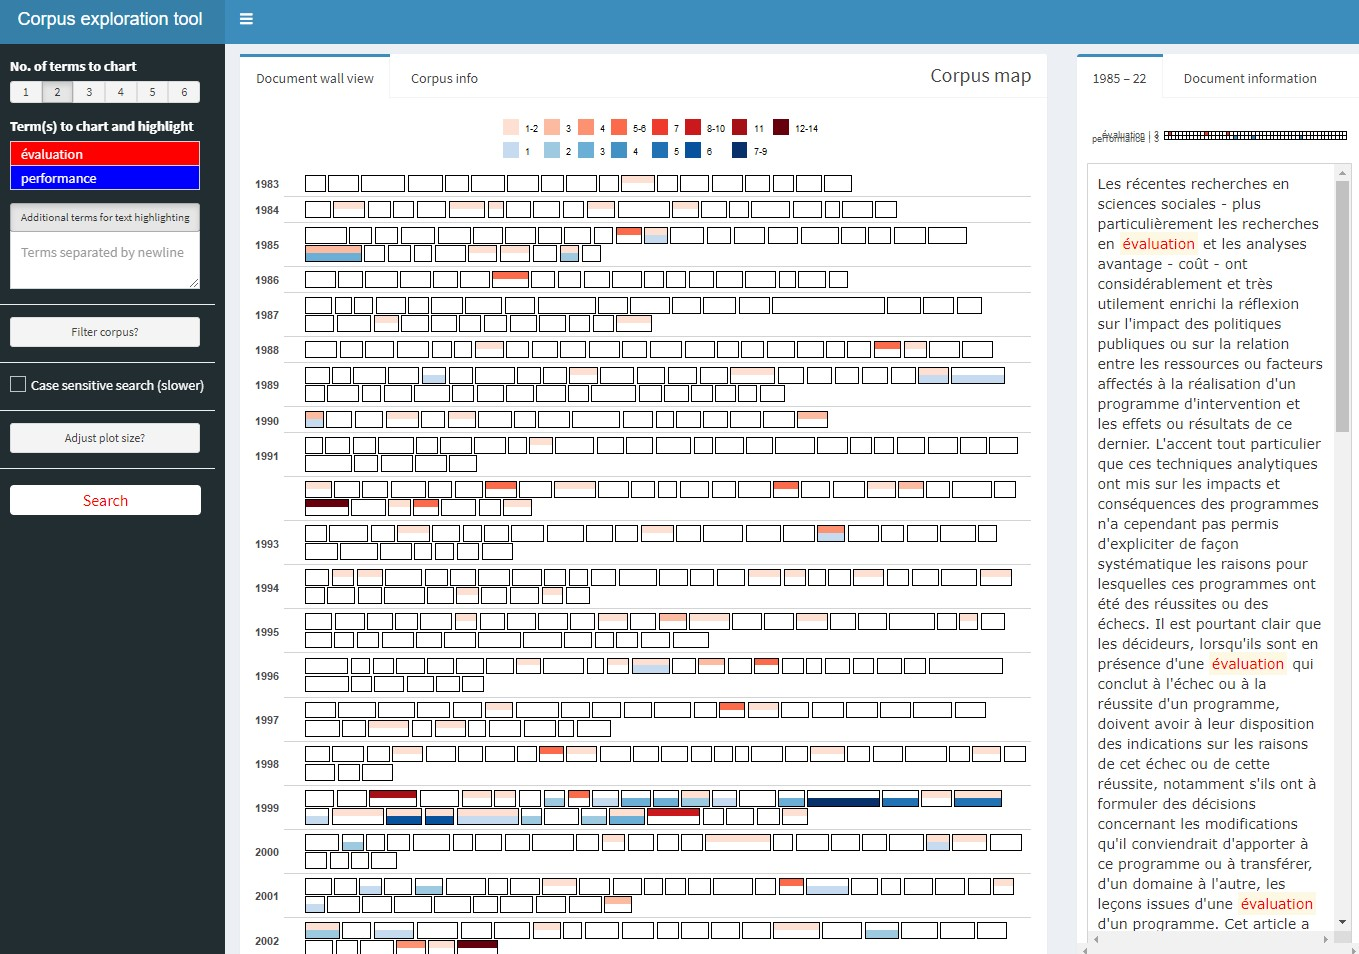
\includegraphics{./image/corpexplor.jpg}

}

\caption{Exploration des abstracts de PMP}

\end{figure}%

\subsection{reprendre le topic de revtools dans topic
model}\label{reprendre-le-topic-de-revtools-dans-topic-model}

https://revtools.net/screening.html\#screening-with-topic-models

\bookmarksetup{startatroot}

\chapter{Manipuler les chaines de
caractères}\label{manipuler-les-chaines-de-caractuxe8res}

\textbf{Objectifs du chapitre :}

\begin{verbatim}
*Apprendre à manipuler les chaines de caractères ainsi que les regex*

</div>
\end{verbatim}

\begin{Shaded}
\begin{Highlighting}[]
\CommentTok{\#les librairies du chapître}
\FunctionTok{library}\NormalTok{(tidyverse)}
\FunctionTok{library}\NormalTok{(readr)}
\FunctionTok{library}\NormalTok{(quanteda)}
\FunctionTok{library}\NormalTok{(flextable)}
\FunctionTok{theme\_set}\NormalTok{(}\FunctionTok{theme\_minimal}\NormalTok{()) }

\FunctionTok{set\_flextable\_defaults}\NormalTok{(}
  \AttributeTok{font.size =} \DecValTok{10}\NormalTok{, }\AttributeTok{theme\_fun =}\NormalTok{ theme\_vanilla,}
  \AttributeTok{padding =} \DecValTok{6}\NormalTok{,}
  \AttributeTok{background.color =} \StringTok{"\#EFEFEF"}\NormalTok{)}


\NormalTok{df }\OtherTok{\textless{}{-}} \FunctionTok{read\_csv}\NormalTok{(}\StringTok{"data/PMPLast3.csv"}\NormalTok{, }
    \AttributeTok{locale =} \FunctionTok{locale}\NormalTok{(}\AttributeTok{encoding =} \StringTok{"WINDOWS{-}1252"}\NormalTok{)) }\SpecialCharTok{\%\textgreater{}\%}
  \FunctionTok{rename}\NormalTok{(}\AttributeTok{Year=}\DecValTok{3}\NormalTok{, }\AttributeTok{Text=}\DecValTok{11}\NormalTok{)}
\end{Highlighting}
\end{Shaded}

\textbf{Environnement de travail}

\section{Stringr}\label{stringr}

\texttt{{[}stringr{]}(https://stringr.tidyverse.org/index.html)} est le
package de la suite tidyverse destiné à manipuler les chaînes de
caractère.

\subsection{Compter}\label{compter}

Dans le code suivant on utilise le set de donnée PMP40ans. Le but est de
compter le nombre de fois où un terme apparaît dans chacun des textes
avec la fonction \texttt{str\_count}. On en donne l'évolution au cours
du temps

\begin{Shaded}
\begin{Highlighting}[]
\NormalTok{foo }\OtherTok{\textless{}{-}}\NormalTok{ df }\SpecialCharTok{\%\textgreater{}\%} 
\NormalTok{  dplyr}\SpecialCharTok{::}\FunctionTok{select}\NormalTok{(Year, Text)}\SpecialCharTok{\%\textgreater{}\%} 
  \FunctionTok{filter}\NormalTok{(}\SpecialCharTok{!}\FunctionTok{is.na}\NormalTok{(Text))}\SpecialCharTok{\%\textgreater{}\%} \CommentTok{\#on filtre les textes manquants}
  \FunctionTok{mutate}\NormalTok{(}\AttributeTok{n=}\FunctionTok{str\_count}\NormalTok{(Text, }\StringTok{"évaluation"}\NormalTok{)) }\SpecialCharTok{\%\textgreater{}\%} \CommentTok{\#}
  \FunctionTok{group\_by}\NormalTok{(Year)}\SpecialCharTok{\%\textgreater{}\%} \CommentTok{\#on agrège sur l\textquotesingle{}année }
  \FunctionTok{summarise}\NormalTok{(}\AttributeTok{n=}\FunctionTok{sum}\NormalTok{(n))}

\FunctionTok{ggplot}\NormalTok{(foo, }\FunctionTok{aes}\NormalTok{(Year,n))}\SpecialCharTok{+}\FunctionTok{geom\_line}\NormalTok{() }\SpecialCharTok{+}
  \FunctionTok{geom\_smooth}\NormalTok{()}\SpecialCharTok{+}
  \FunctionTok{ylim}\NormalTok{(}\DecValTok{0}\NormalTok{,}\DecValTok{40}\NormalTok{)}
\end{Highlighting}
\end{Shaded}

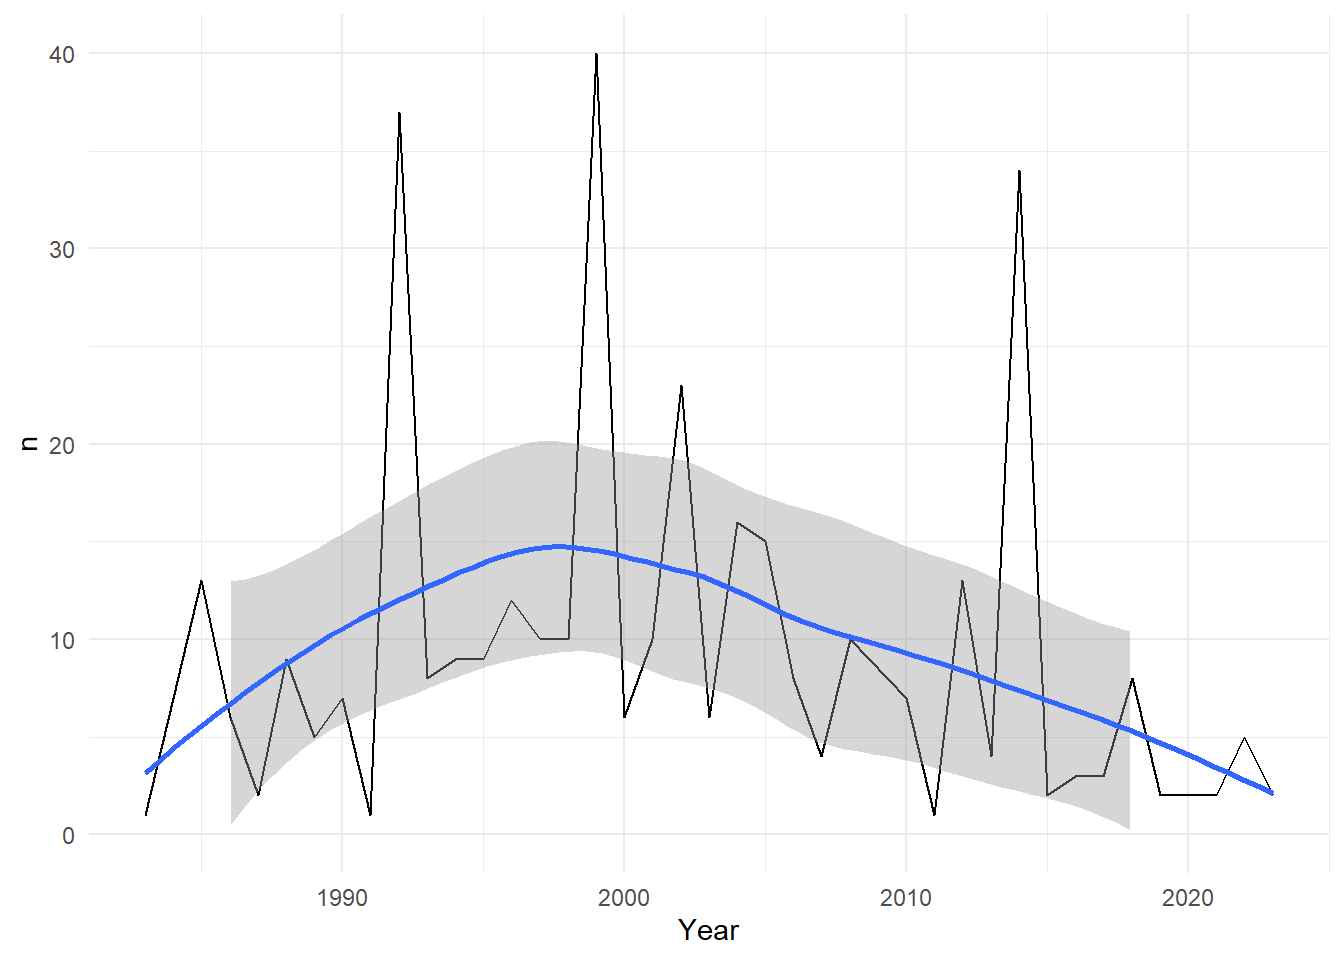
\includegraphics{q05_manipuler_caractere_files/figure-pdf/501-1.pdf}

\subsection{Extraire, supprimer et
remplacer}\label{extraire-supprimer-et-remplacer}

Dans certaines situations on peut souhaiter extraire une chaîne de
caractère pour l'utiliser à un autre usage.L'exemple ordinaire est celui
d'extraire l'année d'une date ou un auteur d'un titre.

\texttt{str\_extract}

\texttt{str\_replace}

\subsection{Majuscules, minuscule et
espaces.}\label{majuscules-minuscule-et-espaces.}

\section{Regex}\label{regex}

Dans la section précédente on a appris à rechercher une chaîne de
caractères, ou plusieurs dans une chaîne de caractères, à les compter,
les extraire, les enlever, les remplacer. Dans nos exemples, on a
employé des pattern simple. Dans l'exemple ``évaluation'', on a tenu
compte uniquement de cette forme, elle aurait pu être au pluriel, porté
une majuscule, exacte ou inexacte. L'enjeu est de pouvoir saisir toute
les variantes en une seule expression.

Dans notre exemple la solution est la suivante :
\texttt{{[}E\textbar{}e\textbar{}é{]}valuation.*}, en voulant saisir
plus de variation on peut employer
\texttt{{[}E\textbar{}e\textbar{}é{]}valu.*} qui permet se saisir les
former verbales.

Une expression régulière, ou regex, ou expression rationnelle ou
expression normale ou motif est une chaîne de caractères qui décrit,
selon une syntaxe précise, un ensemble de chaînes de caractères
possibles. Son invention est attribuée au logicien
\href{https://fr.wikipedia.org/wiki/Stephen_Cole_Kleene}{Stephen Cole
Kleene})

sa pratique se fonde sur une forte théorie.

\subsection{les éléments
principaux}\label{les-uxe9luxe9ments-principaux}

https://towardsdatascience.com/a-gentle-introduction-to-regular-expressions-with-r-df5e897ca432

Les regex reposent sur plusieurs concepts :

\begin{itemize}
\tightlist
\item
  des jeux de caractères qui sont défini par des crochets {[}{]}. Dans
  l'exemple suivant on remplace toutes les voyelles, par rien, puis
  toute les majuscules par X. Il y a différentes variantes par exemple
  {[}A-Z{]} pour les majuscules ou {[}0-9{]} pour les chiffres.
\end{itemize}

\begin{Shaded}
\begin{Highlighting}[]
\CommentTok{\# Mathias Malzieu}
\NormalTok{x}\OtherTok{\textless{}{-}}\FunctionTok{c}\NormalTok{(}\StringTok{"Si Cendrillon avait eu une horloge dans le coeur, elle aurait bloqué les aiguilles à minuit moins une et se serait éclaté au bal toute sa vie."}\NormalTok{)}

\FunctionTok{str\_replace\_all}\NormalTok{(x,}\StringTok{"[aeiou]"}\NormalTok{, }\StringTok{""}\NormalTok{)}
\end{Highlighting}
\end{Shaded}

\begin{verbatim}
[1] "S Cndrlln vt  n hrlg dns l cr, ll rt blqé ls glls à mnt mns n t s srt éclté  bl tt s v."
\end{verbatim}

\begin{Shaded}
\begin{Highlighting}[]
\FunctionTok{str\_replace\_all}\NormalTok{(x,}\StringTok{"[A{-}Z]"}\NormalTok{, }\StringTok{"X"}\NormalTok{)}
\end{Highlighting}
\end{Shaded}

\begin{verbatim}
[1] "Xi Xendrillon avait eu une horloge dans le coeur, elle aurait bloqué les aiguilles à minuit moins une et se serait éclaté au bal toute sa vie."
\end{verbatim}

\begin{itemize}
\tightlist
\item
  Les méta caractères représentent un type de caractère. Ils commencent
  généralement par une barre oblique inverse (backslash). La barre
  oblique inverse étant un caractère spécial dans R, elle doit être
  échappée chaque fois qu'elle est utilisée avec une autre barre oblique
  inverse. En d'autres termes, R exige deux barres obliques inverses
  lors de l'utilisation de méta caractères. Chaque méta-caractère
  correspondra à un seul caractère.
\end{itemize}

\texttt{\textbackslash{}\textbackslash{}s} : Ce méta caractère
représente les espaces. Il correspondra à chaque espace, tabulation et
nouvelle ligne.

\begin{itemize}
\item
  Les quantificateurs permette de contrôler le nombre de caractère que
  l'on attend. Par exemple , le quantificateur + indique que l'on
  souhaite que l'élément recherché apparaisse une ou plus fois. Si
  l'action est d'identifier a, a+, renvoie a, aa, aaa etc . Ceci ne
  semble pas très utile, sauf si le caractère peut être n'importe quelle
  lettre de l'alphabet, ce qui est représenté par le . Une variante du +
  est *, c'est la même idée mais cela inclue l'option de 0 caractère.
\item
  Groupes de capture
\end{itemize}

\subsection{Des formules usuelles}\label{des-formules-usuelles}

La formulation de regex est un art, dans le quotidien on se contentera
de reprendre des formules communes et d'utiliser des générateurs de
regex comme xxxx

en voici quelles-unes

\begin{itemize}
\item
  date
  \texttt{\textbackslash{}{[}0-9\textbackslash{}{]}\{2\}-\textbackslash{}{[}0-9\textbackslash{}{]}\{2\}-\textbackslash{}{[}0-9\textbackslash{}{]}\{2\}"}
\item
  mention
\item
  adresse web
\item
  numéro de téléphone
\end{itemize}

\section{Conclusion}\label{conclusion-3}

Sur le plan pratique nous avons fortement avancé, nous pouvons jouer
avec les chaînes de caractère, et en saisir les variations. nous avons
les moyens de pré-traiter le texte

\begin{itemize}
\tightlist
\item
  pour réduire les morphologies
\item
  pour extraire des entités nommées
\item
  \ldots{}
\end{itemize}

\bookmarksetup{startatroot}

\chapter{Analyse quantitative du
corpus}\label{analyse-quantitative-du-corpus}

\begin{Shaded}
\begin{Highlighting}[]
\CommentTok{\#les librairies du chapître}
\FunctionTok{library}\NormalTok{(tidyverse)}
\CommentTok{\#accessoires de ggplot}
\FunctionTok{library}\NormalTok{(ggridges)}
\FunctionTok{library}\NormalTok{(ggrepel)}
\FunctionTok{library}\NormalTok{(ggwordcloud)}

\FunctionTok{theme\_set}\NormalTok{(}\FunctionTok{theme\_minimal}\NormalTok{()) }

\CommentTok{\#NLP}
\FunctionTok{library}\NormalTok{(tokenizers)}
\FunctionTok{library}\NormalTok{(quanteda)}
\FunctionTok{library}\NormalTok{(quanteda.textplots)}
\FunctionTok{library}\NormalTok{(quanteda.textstats )}
\CommentTok{\#tableau}
\FunctionTok{library}\NormalTok{(flextable)}
\FunctionTok{set\_flextable\_defaults}\NormalTok{(}
  \AttributeTok{font.size =} \DecValTok{10}\NormalTok{, }\AttributeTok{theme\_fun =}\NormalTok{ theme\_vanilla,}
  \AttributeTok{padding =} \DecValTok{6}\NormalTok{,}
  \AttributeTok{background.color =} \StringTok{"\#EFEFEF"}\NormalTok{)}

\CommentTok{\#palettes}

\FunctionTok{library}\NormalTok{(wesanderson)}
\CommentTok{\#names(wes\_palettes)}
\NormalTok{col\_1}\OtherTok{\textless{}{-}}\FunctionTok{c}\NormalTok{(}\StringTok{"\#85D4E3"}\NormalTok{)}
\NormalTok{col\_1b}\OtherTok{\textless{}{-}}\FunctionTok{c}\NormalTok{(}\StringTok{"\#F4B5BD"}\NormalTok{)}
\NormalTok{col\_2}\OtherTok{\textless{}{-}}\NormalTok{c }\OtherTok{\textless{}{-}}\FunctionTok{c}\NormalTok{(}\StringTok{"\#85D4E3"}\NormalTok{, }\StringTok{"\#F4B5BD"}\NormalTok{)}
\NormalTok{col\_4}\OtherTok{\textless{}{-}}\FunctionTok{c}\NormalTok{(}\StringTok{"\#85D4E3"}\NormalTok{, }\StringTok{"\#F4B5BD"}\NormalTok{, }\StringTok{"\#9C964A"}\NormalTok{, }\StringTok{"\#CDC08C"}\NormalTok{)}
\end{Highlighting}
\end{Shaded}

\textbf{Objectifs du chapitre :}

\begin{itemize}
\tightlist
\item
  Avant de se plonger sans l'analyse du lexique on peut étudier le
  corpus de manière quantitative d'autant plus s'il se distribue dans le
  temps. La fréquence des textes, leur longueur, la longueur des mots,
  leur diversité.
\end{itemize}

Une première manière d'aborder un texte ou un corpus est volumétrique.
Quel volume de texte? Quelle longueur ? Combien de mots ? Quelles
variations?

A cette fin on utilise le cas des tweets de Donald Trump. Des premiers
aux derniers, jusqu'au moment de son bannissement en Janvier 2021, après
sa défaite aux élections présidentielles. Chargeons le fichier de
données.( on retrouvera la description du fichier en préambule)

\begin{Shaded}
\begin{Highlighting}[]
\NormalTok{df }\OtherTok{\textless{}{-}} \FunctionTok{read\_csv}\NormalTok{(}\StringTok{"./data/TrumpTwitterArchive01{-}08{-}2021.csv"}\NormalTok{)}
\NormalTok{nrow}\OtherTok{\textless{}{-}}\FunctionTok{nrow}\NormalTok{(df) }\CommentTok{\#nombre de ligne}
\NormalTok{ncol}\OtherTok{\textless{}{-}}\FunctionTok{ncol}\NormalTok{(df) }\CommentTok{\#nombre de colonne}
\NormalTok{df}\SpecialCharTok{$}\NormalTok{nb\_mots}\OtherTok{\textless{}{-}}\FunctionTok{str\_count}\NormalTok{(df}\SpecialCharTok{$}\NormalTok{text, }\StringTok{" "}\NormalTok{)}\SpecialCharTok{+}\DecValTok{1} \CommentTok{\# l\textquotesingle{}astuce : compter les espaces et ajouter 1, pour compter les mots}
\NormalTok{sum\_mots}\OtherTok{\textless{}{-}}\FunctionTok{sum}\NormalTok{(df}\SpecialCharTok{$}\NormalTok{nb\_mots)             }\CommentTok{\#ON COMPTE LE NOMBRE DE MOTS}
\end{Highlighting}
\end{Shaded}

\section{Comptons les mots}\label{comptons-les-mots}

Il y 56571 tweets et 9 variables et \ensuremath{1.117018\times 10^{6}}
mots cumulés.

On peut vouloir compter le nombre de mots. A cette fin on emploie une
fonction de \texttt{stringr}, un package précieux que nous allons
étudier de plus dans le chapitres suivant : \texttt{str\_count}.

On note immédiatement la bi-modalité de la distribution qui correspond
au changement de règle par Twitter en matière de non de caractères
utilisés, étendu de 180 à 280.

\begin{Shaded}
\begin{Highlighting}[]
\FunctionTok{ggplot}\NormalTok{(df, }\FunctionTok{aes}\NormalTok{(}\AttributeTok{x=}\NormalTok{nb\_mots))}\SpecialCharTok{+}
  \FunctionTok{geom\_histogram}\NormalTok{(}\AttributeTok{fill=}\NormalTok{col\_1, }\AttributeTok{binwidth =} \DecValTok{10}\NormalTok{)}\SpecialCharTok{+}
  \FunctionTok{labs}\NormalTok{(}\AttributeTok{title=}\FunctionTok{paste0}\NormalTok{(}\StringTok{"Nombre total de mots du corpus : "}\NormalTok{,sum\_mots), }
       \AttributeTok{x=}\StringTok{"Nombre de mots par post"}\NormalTok{, }
       \AttributeTok{y=}\StringTok{"Fréquence"}\NormalTok{)}
\end{Highlighting}
\end{Shaded}

\includegraphics{q06_Analyse_quantitative_files/figure-pdf/602-1.pdf}

La bimodalité provient surement du changement de taille maximum effectué
en septembre 2017, le passage de 180 caractères max à 280. On peut le
vérifier en examinant cette même distribution - par les courbes de
densité - pour chacune des années, avec cette technique rendue fameuse
par la pochette de l'album de Joy Division : un graphique en crêtes
(ridges plot) avec
\href{https://cran.r-project.org/web/packages/ggridges/vignettes/introduction.html}{\texttt{ggridges}}.

Le résultat remarquable est que si Trump dans un premier temps exploite
cette nouvel fonctionnalité, il en revient avec un phrasé de 20 mots en
moyenne, gardant cependant à l'occasion d'autre contenu en 50 mots
environ.

\begin{Shaded}
\begin{Highlighting}[]
\NormalTok{df}\SpecialCharTok{$}\NormalTok{Year}\OtherTok{\textless{}{-}}\FunctionTok{format}\NormalTok{(df}\SpecialCharTok{$}\NormalTok{date, }\AttributeTok{format =} \StringTok{"\%Y"}\NormalTok{) }\CommentTok{\#on extrait l\textquotesingle{}année de la date}
\NormalTok{foo}\OtherTok{\textless{}{-}}\NormalTok{ df }\SpecialCharTok{\%\textgreater{}\%} 
  \FunctionTok{filter}\NormalTok{(Year}\SpecialCharTok{!=}\StringTok{"2021"}\NormalTok{) }\CommentTok{\#parce qu\textquotesingle{}il n\textquotesingle{}y a quelques quelques jours en janvier, le compte a été interrompu vers le 5 janavier}

\FunctionTok{ggplot}\NormalTok{(foo,}\FunctionTok{aes}\NormalTok{(}\AttributeTok{x =}\NormalTok{ nb\_mots, }\AttributeTok{y =}\NormalTok{ Year, }\AttributeTok{group =}\NormalTok{ Year)) }\SpecialCharTok{+}
  \FunctionTok{geom\_density\_ridges}\NormalTok{(}\AttributeTok{scale =} \DecValTok{4}\NormalTok{, }\AttributeTok{color=}\StringTok{"grey90"}\NormalTok{,}\AttributeTok{fill=}\NormalTok{col\_1, }\AttributeTok{alpha=}\NormalTok{.}\DecValTok{7}\NormalTok{)}\SpecialCharTok{+}
  \FunctionTok{theme\_ridges}\NormalTok{() }\SpecialCharTok{+}
  \FunctionTok{scale\_x\_continuous}\NormalTok{(}\AttributeTok{limits =} \FunctionTok{c}\NormalTok{(}\DecValTok{1}\NormalTok{, }\DecValTok{60}\NormalTok{)) }\SpecialCharTok{+}
  \FunctionTok{labs}\NormalTok{(}\AttributeTok{x=}\StringTok{"Nombre de mots par post"}\NormalTok{,}
       \AttributeTok{y=}\ConstantTok{NULL}\NormalTok{)}
\end{Highlighting}
\end{Shaded}

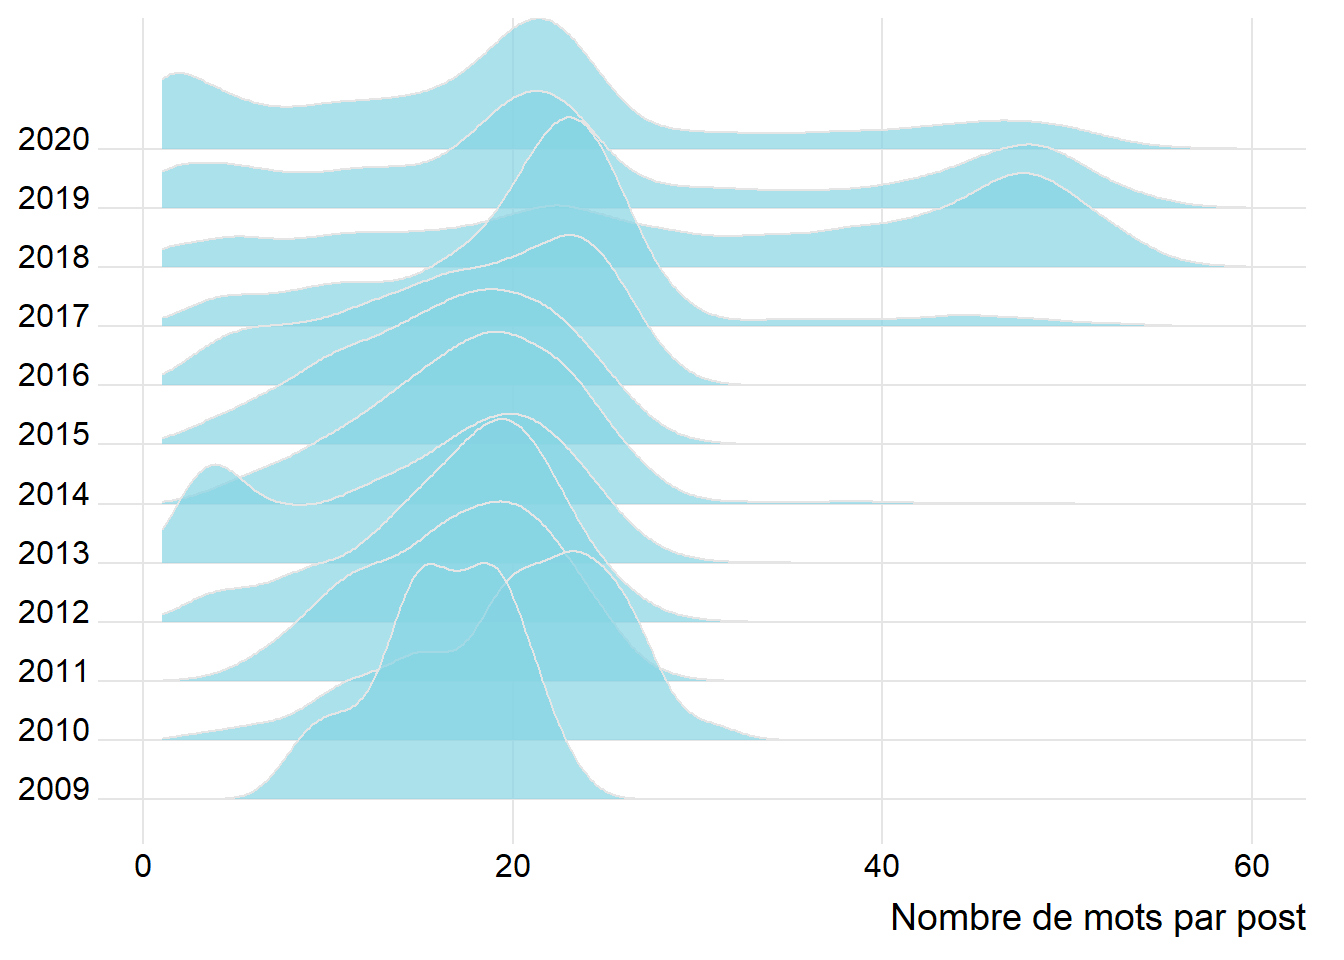
\includegraphics{q06_Analyse_quantitative_files/figure-pdf/603-1.pdf}

\section{La production dans le temps}\label{la-production-dans-le-temps}

Examinons le nombre de tweets produit au cours du temps.

On se rappellera qu'après une carrière immobilière menée dans les
casinos, le golf et les hôtels, l'appétit médiatique de Trump s'est
réalisé dans ``the apprentice'', de 2004 à 2015. C'est un pro de la TV,
il a une formation de Popstar. Il sera élu en Décembre 2016 pour prendre
le pouvoir en Janvier.

\begin{Shaded}
\begin{Highlighting}[]
\NormalTok{df}\SpecialCharTok{$}\NormalTok{date2}\OtherTok{\textless{}{-}}\FunctionTok{format}\NormalTok{(df}\SpecialCharTok{$}\NormalTok{date, }\StringTok{"\%Y{-}\%m{-}\%d"}\NormalTok{)}
\NormalTok{df}\SpecialCharTok{$}\NormalTok{date3}\OtherTok{\textless{}{-}}\FunctionTok{as.POSIXct}\NormalTok{(df}\SpecialCharTok{$}\NormalTok{date2, }\AttributeTok{format =} \StringTok{"\%Y{-}\%m{-}\%d"}\NormalTok{)}
\NormalTok{df}\SpecialCharTok{$}\NormalTok{isRetweet}\OtherTok{\textless{}{-}}\FunctionTok{as.character}\NormalTok{(df}\SpecialCharTok{$}\NormalTok{isRetweet)}

\NormalTok{foo}\OtherTok{\textless{}{-}}\NormalTok{df }\SpecialCharTok{\%\textgreater{}\%} \FunctionTok{filter}\NormalTok{(Year}\SpecialCharTok{!=}\DecValTok{2021}\NormalTok{)}\SpecialCharTok{\%\textgreater{}\%}
  \FunctionTok{group\_by}\NormalTok{(date3, isRetweet)}\SpecialCharTok{\%\textgreater{}\%}
  \FunctionTok{summarise}\NormalTok{(}\AttributeTok{n=}\FunctionTok{n}\NormalTok{())}

\DocumentationTok{\#\# plot time series of tweets}

\FunctionTok{ggplot}\NormalTok{(foo, }\FunctionTok{aes}\NormalTok{(}\AttributeTok{x=}\NormalTok{date3, }\AttributeTok{y=}\NormalTok{n,}\AttributeTok{group=}\NormalTok{isRetweet))}\SpecialCharTok{+}
  \FunctionTok{geom\_line}\NormalTok{(}\FunctionTok{aes}\NormalTok{(}\AttributeTok{color=}\NormalTok{isRetweet), }\AttributeTok{alpha=}\NormalTok{.}\DecValTok{2}\NormalTok{)}\SpecialCharTok{+}
  \FunctionTok{geom\_smooth}\NormalTok{(}\FunctionTok{aes}\NormalTok{(}\AttributeTok{color=}\NormalTok{isRetweet),}\AttributeTok{span=}\FloatTok{0.5}\NormalTok{)}\SpecialCharTok{+}
    \FunctionTok{scale\_x\_datetime}\NormalTok{(}\AttributeTok{date\_breaks =} \StringTok{"1 year"}\NormalTok{, }\AttributeTok{labels =}\NormalTok{ scales}\SpecialCharTok{::}\FunctionTok{label\_date\_short}\NormalTok{())}\SpecialCharTok{+}
  \FunctionTok{labs}\NormalTok{(}\AttributeTok{y=}\StringTok{"nombre de tweets par jour"}\NormalTok{, }\AttributeTok{x=}\ConstantTok{NULL}\NormalTok{)}\SpecialCharTok{+}
  \FunctionTok{scale\_color\_manual}\NormalTok{(}\AttributeTok{values =}\NormalTok{ col\_2)}
\end{Highlighting}
\end{Shaded}

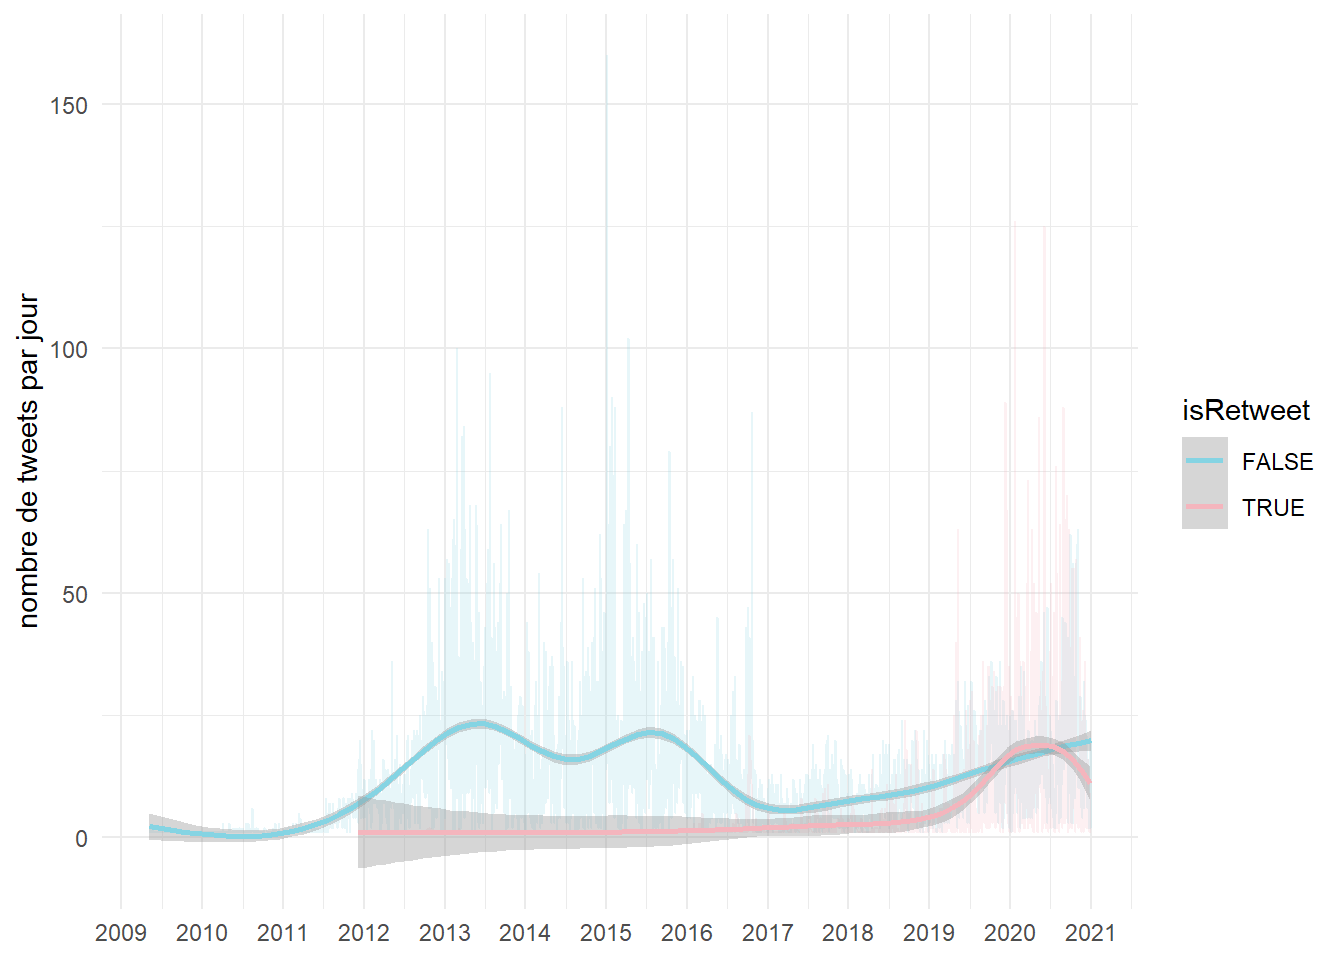
\includegraphics{q06_Analyse_quantitative_files/figure-pdf/604-1.pdf}

\begin{Shaded}
\begin{Highlighting}[]
\CommentTok{\#raf : labeliser avec les dates clés}
\end{Highlighting}
\end{Shaded}

\section{Popularité des tweets}\label{popularituxe9-des-tweets}

Dans ce set de donnée si l'auteur est unique, la réception est multiple,
rappelons que près de 90 millions de personnes suivaient Trump. On
possède deux indicateurs : le nombre de retweet et de RT.

\begin{Shaded}
\begin{Highlighting}[]
\NormalTok{foo}\OtherTok{\textless{}{-}}\NormalTok{df }\SpecialCharTok{\%\textgreater{}\%} \FunctionTok{select}\NormalTok{(Year, favorites, retweets)}\SpecialCharTok{\%\textgreater{}\%}
  \FunctionTok{filter}\NormalTok{(}\SpecialCharTok{!}\FunctionTok{is.na}\NormalTok{(favorites) }\SpecialCharTok{\&}\NormalTok{ Year}\SpecialCharTok{!=}\DecValTok{2021}\NormalTok{)}\SpecialCharTok{\%\textgreater{}\%}
  \FunctionTok{group\_by}\NormalTok{(Year)}\SpecialCharTok{\%\textgreater{}\%}
  \FunctionTok{summarize}\NormalTok{(}\AttributeTok{sum\_rt=}\FunctionTok{sum}\NormalTok{(retweets),}
            \AttributeTok{sum\_fav=}\FunctionTok{sum}\NormalTok{(favorites),}
            \AttributeTok{mean\_rt=}\FunctionTok{mean}\NormalTok{(retweets),}
            \AttributeTok{mean\_fav=}\FunctionTok{mean}\NormalTok{(favorites)}
\NormalTok{            ) }\SpecialCharTok{\%\textgreater{}\%}
  \FunctionTok{pivot\_longer}\NormalTok{(}\SpecialCharTok{{-}}\NormalTok{Year,}\AttributeTok{names\_to =} \StringTok{"variable"}\NormalTok{, }\AttributeTok{values\_to =} \StringTok{"values"}\NormalTok{)}

\FunctionTok{ggplot}\NormalTok{(foo, }\FunctionTok{aes}\NormalTok{(}\AttributeTok{x=}\NormalTok{Year, }\AttributeTok{y=}\NormalTok{values,}\AttributeTok{group=}\NormalTok{variable))}\SpecialCharTok{+}
  \FunctionTok{geom\_line}\NormalTok{(}\FunctionTok{aes}\NormalTok{(}\AttributeTok{color=}\NormalTok{variable), }\AttributeTok{size=}\DecValTok{1}\NormalTok{,}\AttributeTok{alpha=}\NormalTok{.}\DecValTok{8}\NormalTok{)}\SpecialCharTok{+}
  \FunctionTok{labs}\NormalTok{(}\AttributeTok{y=}\StringTok{"nombre de tweets par jour"}\NormalTok{, }\AttributeTok{x=}\ConstantTok{NULL}\NormalTok{)}\SpecialCharTok{+}
  \FunctionTok{scale\_color\_manual}\NormalTok{(}\AttributeTok{values =}\NormalTok{ col\_4)}\SpecialCharTok{+} 
  \FunctionTok{facet\_wrap}\NormalTok{(}\FunctionTok{vars}\NormalTok{(variable), }\AttributeTok{ncol=}\DecValTok{2}\NormalTok{, }\AttributeTok{scale=}\StringTok{"free"}\NormalTok{)}\SpecialCharTok{+}
  \FunctionTok{scale\_y\_log10}\NormalTok{()}
\end{Highlighting}
\end{Shaded}

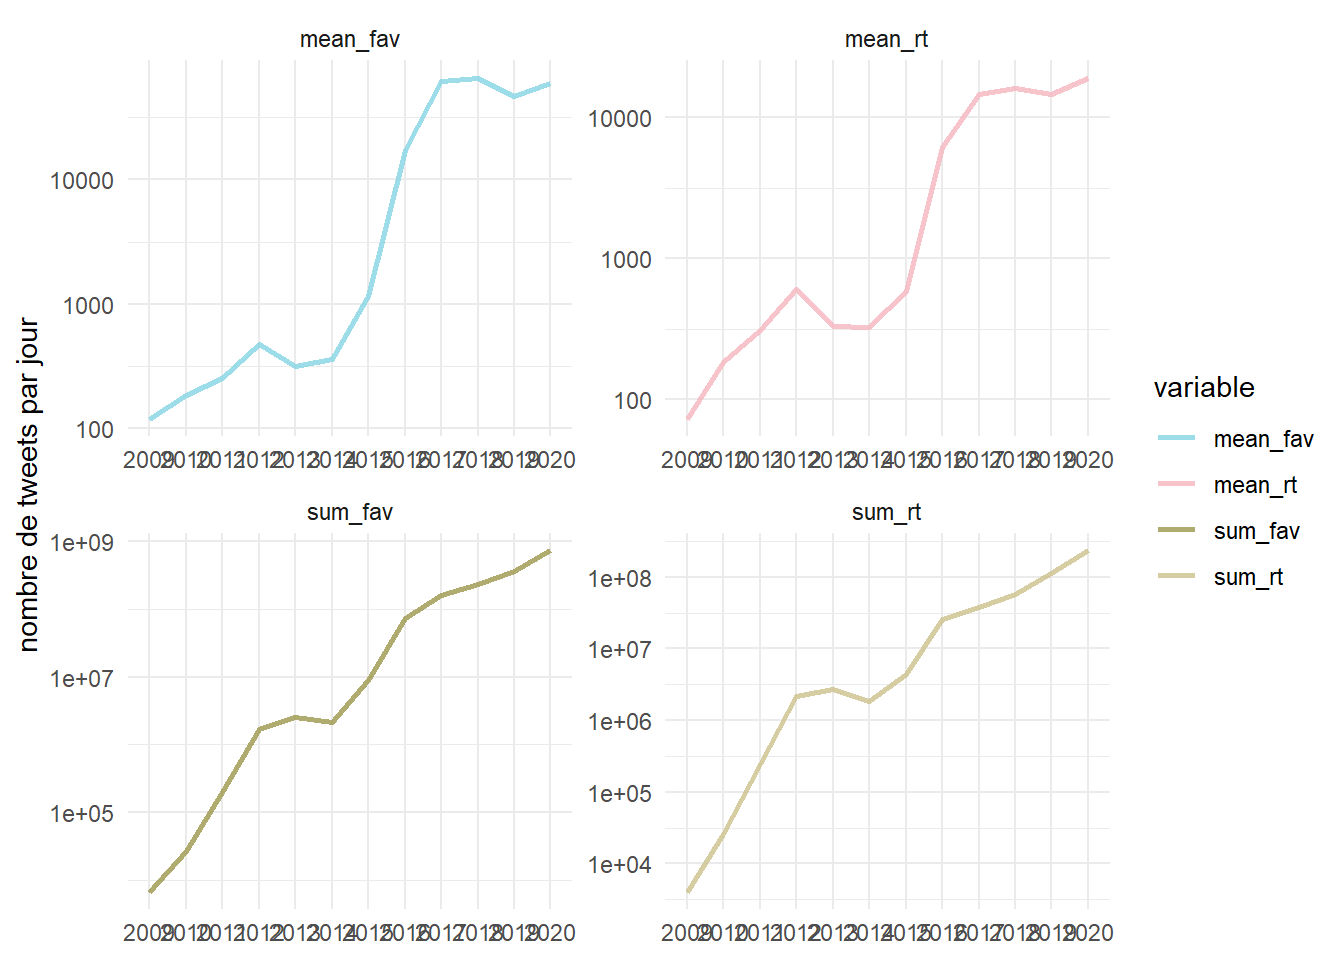
\includegraphics{q06_Analyse_quantitative_files/figure-pdf/605-1.pdf}

On s'aperçoit d'un changement de régime, quand l'audience est limitée RT
et fac sont fortement corrélés, l'entrée en politique de Trump se
caractérise par un changement de régime. La décorrélation peut
s'expliquer par l'usage d'agent d'influences, qui retweetent plus qu'ils
n'approuvent. Ils contribuent à la décorrélation.

\begin{Shaded}
\begin{Highlighting}[]
\NormalTok{foo}\OtherTok{\textless{}{-}}\NormalTok{df }\SpecialCharTok{\%\textgreater{}\%} \FunctionTok{select}\NormalTok{(Year, favorites, retweets)}\SpecialCharTok{\%\textgreater{}\%}
  \FunctionTok{filter}\NormalTok{(}\SpecialCharTok{!}\FunctionTok{is.na}\NormalTok{(favorites) }\SpecialCharTok{\&}\NormalTok{ Year}\SpecialCharTok{!=}\DecValTok{2021}\NormalTok{)}\SpecialCharTok{\%\textgreater{}\%}
  \FunctionTok{group\_by}\NormalTok{(Year)}\SpecialCharTok{\%\textgreater{}\%}
  \FunctionTok{summarize}\NormalTok{(}\FunctionTok{cor}\NormalTok{(favorites, retweets)) }\SpecialCharTok{\%\textgreater{}\%}
  \FunctionTok{rename}\NormalTok{(}\AttributeTok{correlation =}\DecValTok{2}\NormalTok{)}
            
\FunctionTok{ggplot}\NormalTok{(foo, }\FunctionTok{aes}\NormalTok{(}\AttributeTok{x=}\NormalTok{Year, }\AttributeTok{y=}\NormalTok{correlation, }\AttributeTok{group=}\DecValTok{1}\NormalTok{))}\SpecialCharTok{+}
  \FunctionTok{geom\_line}\NormalTok{(}\AttributeTok{size=}\DecValTok{1}\NormalTok{,}\AttributeTok{alpha=}\NormalTok{.}\DecValTok{8}\NormalTok{, }\AttributeTok{color=}\NormalTok{col\_1b)}\SpecialCharTok{+}
  \FunctionTok{geom\_smooth}\NormalTok{(}\AttributeTok{color=}\NormalTok{col\_1b, }\AttributeTok{size=}\FloatTok{1.5}\NormalTok{, }\AttributeTok{fill=}\StringTok{"grey90"}\NormalTok{)}\SpecialCharTok{+}
  \FunctionTok{labs}\NormalTok{(}\AttributeTok{y=}\StringTok{"Corrélation entre fav et rt"}\NormalTok{, }\AttributeTok{x=}\ConstantTok{NULL}\NormalTok{)}
\end{Highlighting}
\end{Shaded}

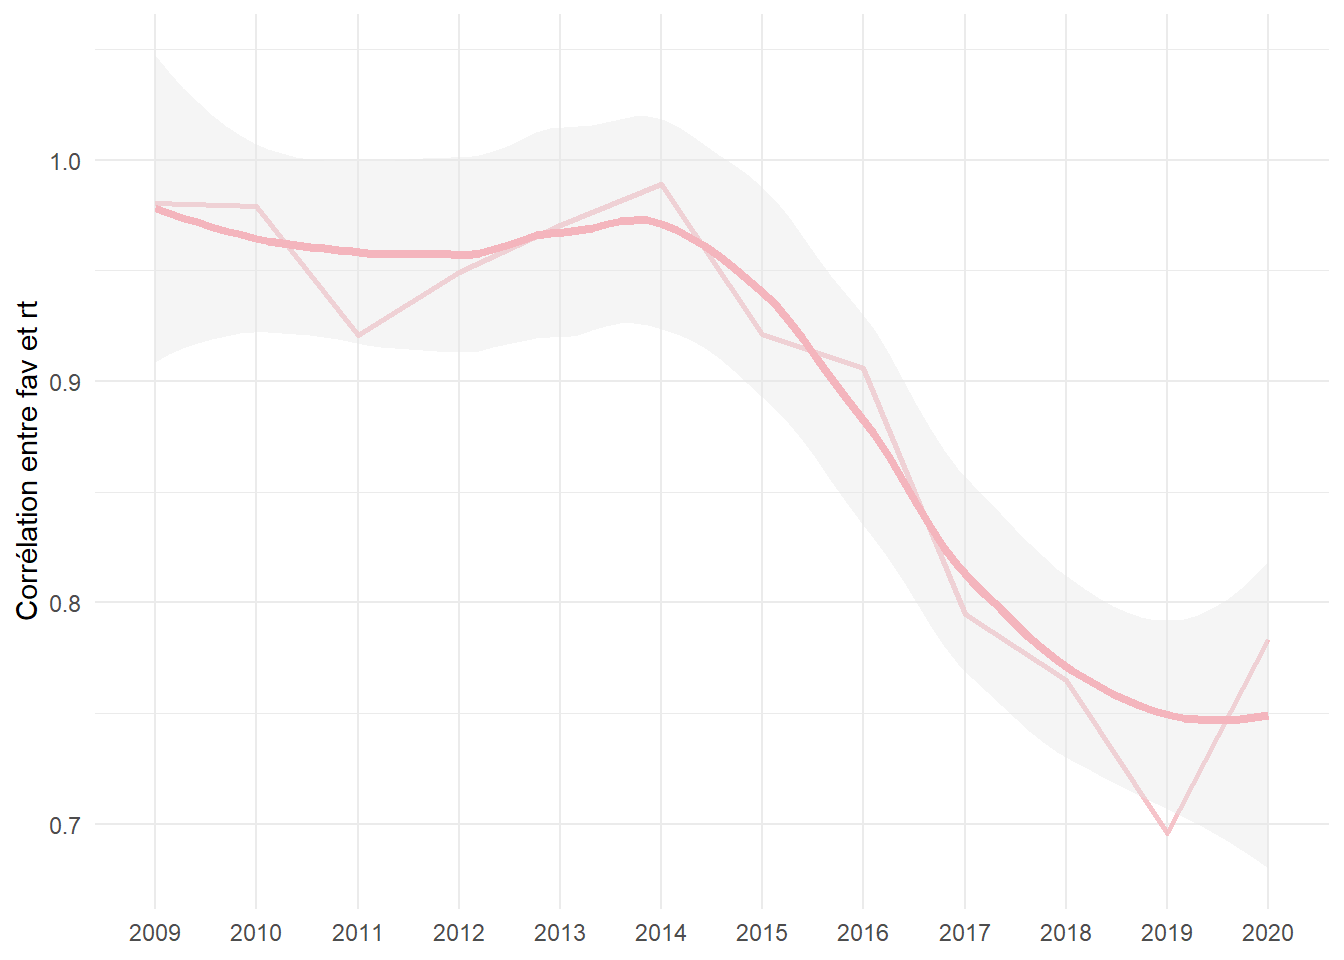
\includegraphics{q06_Analyse_quantitative_files/figure-pdf/606-1.pdf}

\begin{Shaded}
\begin{Highlighting}[]
\NormalTok{foo}\OtherTok{\textless{}{-}}\NormalTok{df }\SpecialCharTok{\%\textgreater{}\%} \FunctionTok{select}\NormalTok{(Year, favorites, retweets)}\SpecialCharTok{\%\textgreater{}\%}
  \FunctionTok{filter}\NormalTok{(}\SpecialCharTok{!}\FunctionTok{is.na}\NormalTok{(favorites) }\SpecialCharTok{\&}\NormalTok{ Year}\SpecialCharTok{==}\DecValTok{2020}\NormalTok{)}


\NormalTok{m }\OtherTok{\textless{}{-}} \FunctionTok{ggplot}\NormalTok{(foo, }\FunctionTok{aes}\NormalTok{(}\AttributeTok{x =}\NormalTok{ favorites, }\AttributeTok{y =}\NormalTok{ retweets)) }\SpecialCharTok{+}
 \FunctionTok{geom\_point}\NormalTok{() }\SpecialCharTok{+}
\FunctionTok{scale\_x\_log10}\NormalTok{()}\SpecialCharTok{+}
\FunctionTok{scale\_y\_log10}\NormalTok{()}

\CommentTok{\# contour lines}
\NormalTok{m }\SpecialCharTok{+} \FunctionTok{geom\_density\_2d}\NormalTok{()}
\end{Highlighting}
\end{Shaded}

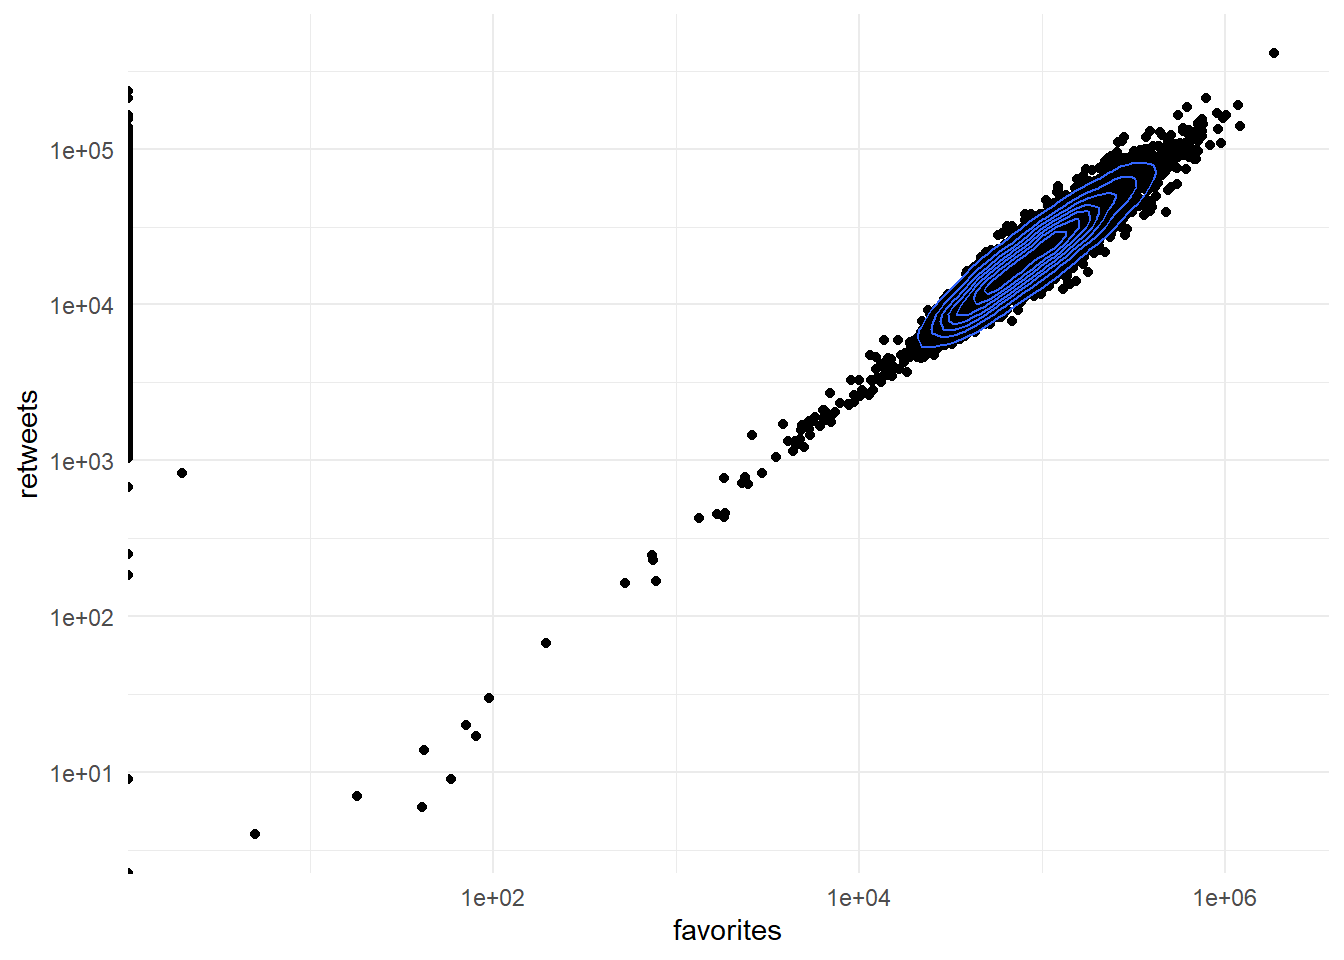
\includegraphics{q06_Analyse_quantitative_files/figure-pdf/607-1.pdf}

\begin{Shaded}
\begin{Highlighting}[]
\NormalTok{df}\SpecialCharTok{$}\NormalTok{date2}\OtherTok{\textless{}{-}}\FunctionTok{format}\NormalTok{(df}\SpecialCharTok{$}\NormalTok{date, }\StringTok{"\%Y{-}\%m{-}\%d"}\NormalTok{)}
\NormalTok{df}\SpecialCharTok{$}\NormalTok{date3}\OtherTok{\textless{}{-}}\FunctionTok{as.POSIXct}\NormalTok{(df}\SpecialCharTok{$}\NormalTok{date2, }\AttributeTok{format =} \StringTok{"\%Y{-}\%m{-}\%d"}\NormalTok{)}
\NormalTok{df}\SpecialCharTok{$}\NormalTok{isRetweet}\OtherTok{\textless{}{-}}\FunctionTok{as.character}\NormalTok{(df}\SpecialCharTok{$}\NormalTok{isRetweet)}

\NormalTok{foo}\OtherTok{\textless{}{-}}\NormalTok{df }\SpecialCharTok{\%\textgreater{}\%} \FunctionTok{filter}\NormalTok{(Year}\SpecialCharTok{!=}\DecValTok{2021}\NormalTok{)}\SpecialCharTok{\%\textgreater{}\%}
  \FunctionTok{group\_by}\NormalTok{(date3, isRetweet)}\SpecialCharTok{\%\textgreater{}\%}
  \FunctionTok{summarise}\NormalTok{(}\AttributeTok{n=}\FunctionTok{n}\NormalTok{())}

\DocumentationTok{\#\# plot time series of tweets}

\FunctionTok{ggplot}\NormalTok{(foo, }\FunctionTok{aes}\NormalTok{(}\AttributeTok{x=}\NormalTok{date3, }\AttributeTok{y=}\NormalTok{n,}\AttributeTok{group=}\NormalTok{isRetweet))}\SpecialCharTok{+}
  \FunctionTok{geom\_line}\NormalTok{(}\FunctionTok{aes}\NormalTok{(}\AttributeTok{color=}\NormalTok{isRetweet), }\AttributeTok{alpha=}\NormalTok{.}\DecValTok{2}\NormalTok{)}\SpecialCharTok{+}
  \FunctionTok{geom\_smooth}\NormalTok{(}\FunctionTok{aes}\NormalTok{(}\AttributeTok{color=}\NormalTok{isRetweet),}\AttributeTok{span=}\FloatTok{0.5}\NormalTok{)}\SpecialCharTok{+}
    \FunctionTok{scale\_x\_datetime}\NormalTok{(}\AttributeTok{date\_breaks =} \StringTok{"1 year"}\NormalTok{, }\AttributeTok{labels =}\NormalTok{ scales}\SpecialCharTok{::}\FunctionTok{label\_date\_short}\NormalTok{())}\SpecialCharTok{+}
  \FunctionTok{labs}\NormalTok{(}\AttributeTok{y=}\StringTok{"nombre de tweets par jour"}\NormalTok{, }\AttributeTok{x=}\ConstantTok{NULL}\NormalTok{)}\SpecialCharTok{+}
  \FunctionTok{scale\_color\_manual}\NormalTok{(}\AttributeTok{values =}\NormalTok{ col\_2)}
\end{Highlighting}
\end{Shaded}

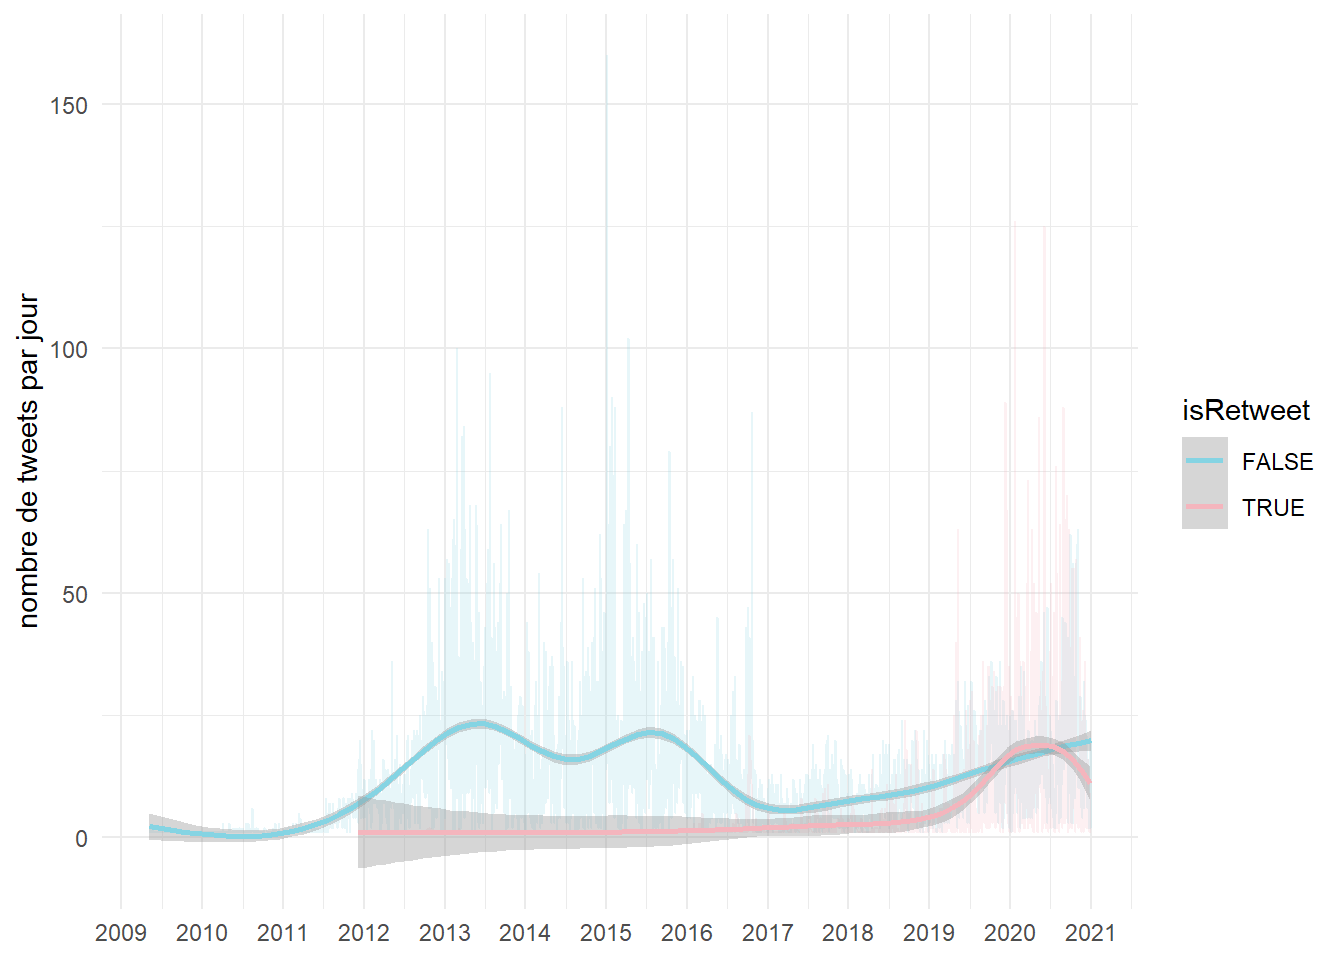
\includegraphics{q06_Analyse_quantitative_files/figure-pdf/608-1.pdf}

\begin{Shaded}
\begin{Highlighting}[]
\CommentTok{\#raf : labeliser avec les dates clés}
\end{Highlighting}
\end{Shaded}

\section{Lisibilité et complexité
lexicale}\label{lisibilituxe9-et-complexituxe9-lexicale}

Pour aller un peu plus loin - nous savons désormais que Trump aime une
forme courte en 21 mots, et que son expérience de twitter est longue, on
peut s'intéresser à des paramètres clés relatifs aux conditions de la
réception: les textes sont-ils aisés à lire ? sont-ils sophistiqués ?

Introduisons deux quantifications utiles du texte : la lisibilité et la
complexité lexicale. Ce sont des classiques, les critères initiaux de
l'analyse quantitative du texte. Ils sont toujours utiles.

\subsection{Les indices de
lisibilité}\label{les-indices-de-lisibilituxe9}

La lisibilité est une notion ancienne tout autant que sa mesure (par
exemple Coleman and Liau (1975)). Elle répond à la question du degré de
maîtrise requis pour lire un texte en s'appuyant sur les
caractéristiques objectives du texte plutôt que sur sa perception. Il
s'agissait donc d'évaluer la complexité d'un texte à partir de deux
critères : la complexité des mots capturée par le nombre moyen de
syllabes, et la complexité des phrases mesurée par le nombre de mots.

A partir de ces deux paramètres, une multitudes d'indicateurs ont été
proposés. Dans l'exemple qui va suivre, on se contente d'un grand
classique, le plus ancien, l'indice de Flesch (Flesch 1948) et de ses
constituants : le nombre moyen de syllabes par mot et le nombre moyen de
mots par phrase.

On les retrouve, avec une autre grande variété, dans le package
compagnon de quanteda ,
\href{https://quanteda.io/reference/textstat_readability.html}{\texttt{quanteda.textstats}}
, qui en fournit des dizaines de variantes.

\begin{Shaded}
\begin{Highlighting}[]
\CommentTok{\#on sélectionne les tweets originaux}

\NormalTok{foo}\OtherTok{\textless{}{-}}\NormalTok{df }\SpecialCharTok{\%\textgreater{}\%} \FunctionTok{filter}\NormalTok{(isRetweet}\SpecialCharTok{==}\ConstantTok{FALSE}\NormalTok{) }\CommentTok{\# on ne prend pas en compte les RT}

\CommentTok{\#la fonction de calcul de lisibilité}
\NormalTok{readability}\OtherTok{\textless{}{-}}\FunctionTok{textstat\_readability}\NormalTok{(foo}\SpecialCharTok{$}\NormalTok{text, }
                                  \AttributeTok{measure =} \FunctionTok{c}\NormalTok{(}\StringTok{"Flesch"}\NormalTok{,}\StringTok{"meanSentenceLength"}\NormalTok{, }\StringTok{"meanWordSyllables"}\NormalTok{),}
                                  \AttributeTok{min\_sentence\_length =} \DecValTok{3}\NormalTok{,}
                                  \AttributeTok{max\_sentence\_length =} \DecValTok{1000}\NormalTok{) }
\CommentTok{\# on joint les données}
\NormalTok{foo}\OtherTok{\textless{}{-}}\FunctionTok{cbind}\NormalTok{(foo,readability[,}\DecValTok{2}\SpecialCharTok{:}\DecValTok{4}\NormalTok{])}

\CommentTok{\#on agrège par année}
\NormalTok{foo1}\OtherTok{\textless{}{-}}\NormalTok{foo }\SpecialCharTok{\%\textgreater{}\%} \FunctionTok{filter}\NormalTok{(Year}\SpecialCharTok{!=}\DecValTok{2021}\NormalTok{) }\SpecialCharTok{\%\textgreater{}\%}
  \FunctionTok{group\_by}\NormalTok{(Year) }\SpecialCharTok{\%\textgreater{}\%}
  \FunctionTok{summarise}\NormalTok{(}\AttributeTok{all\_tweet=}\FunctionTok{n}\NormalTok{(),}
            \AttributeTok{Flesch=}\FunctionTok{mean}\NormalTok{(Flesch, }\AttributeTok{na.rm=}\ConstantTok{TRUE}\NormalTok{), }
            \AttributeTok{SentenceLength=} \FunctionTok{mean}\NormalTok{(meanSentenceLength, }\AttributeTok{na.rm=}\ConstantTok{TRUE}\NormalTok{),}
            \AttributeTok{WordSyllables=} \FunctionTok{mean}\NormalTok{(meanWordSyllables, }\AttributeTok{na.rm=}\ConstantTok{TRUE}\NormalTok{)) }\SpecialCharTok{\%\textgreater{}\%}
  \FunctionTok{gather}\NormalTok{(variable, value, }\SpecialCharTok{{-}}\NormalTok{Year)}

\CommentTok{\#visualisation}

\FunctionTok{ggplot}\NormalTok{(foo1,}\FunctionTok{aes}\NormalTok{(}\AttributeTok{x=}\NormalTok{Year, }\AttributeTok{y=}\NormalTok{value, }\AttributeTok{group=}\NormalTok{variable))}\SpecialCharTok{+}
  \FunctionTok{geom\_line}\NormalTok{(}\AttributeTok{size=}\FloatTok{1.2}\NormalTok{, }\FunctionTok{aes}\NormalTok{(}\AttributeTok{color=}\NormalTok{variable), }\AttributeTok{stat=}\StringTok{"identity"}\NormalTok{)}\SpecialCharTok{+}
  \FunctionTok{facet\_wrap}\NormalTok{(}\FunctionTok{vars}\NormalTok{(variable), }\AttributeTok{scale=}\StringTok{"free"}\NormalTok{, }\AttributeTok{ncol=}\DecValTok{1}\NormalTok{)}\SpecialCharTok{+}
  \FunctionTok{labs}\NormalTok{(}\AttributeTok{title =} \StringTok{"Evolution de la lisibilité des tweets de Trump"}\NormalTok{, }\AttributeTok{x=}\ConstantTok{NULL}\NormalTok{, }\AttributeTok{y=}\ConstantTok{NULL}\NormalTok{)}
\end{Highlighting}
\end{Shaded}

\includegraphics{q06_Analyse_quantitative_files/figure-pdf/609-1.pdf}

Pour aider le lecteur à donner un sens, voici l'abaque proposée par
\href{http://www.appstate.edu/~steelekm/classes/psy2664/Flesch.htm}{Flesch}
lui-même.

\begin{figure}[H]

{\centering 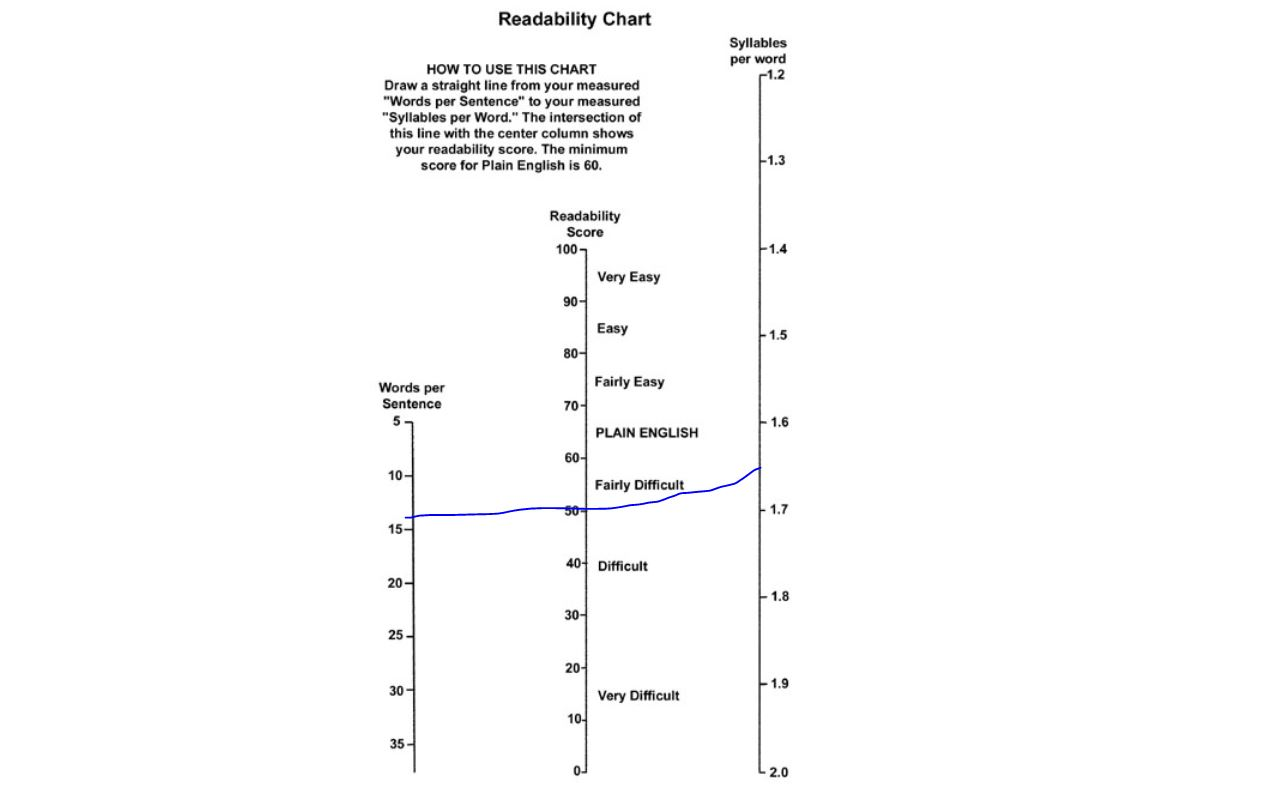
\includegraphics{./image/ReadabilityFlesch.JPG}

}

\caption{Flesch}

\end{figure}%

On peut aussi prendre pour références les éléments suivants:

``All Plain English examples in this book score at least 60. Here are
the scores of some reading materials I've tested. These are average
scores of random samples.'' ( source ?)

\begin{itemize}
\item
  Comics 92
\item
  Consumer ads in magazines 82
\item
  Reader's Digest 65
\item
  Time 52
\item
  Wall Street Journal 43
\item
  Harvard Business Review 43
\item
  Harvard Law Review 32
\item
  Auto insurance policy 10
\end{itemize}

Trump ne parait pas être sa caricature, non niveau de lisibilité
correspond à la Licence. Le Reader's Digest est beaucoup plus simple, il
se situe au dessus de la Harvard Business Review !

\subsection{Les indices de complexité
lexicale}\label{les-indices-de-complexituxe9-lexicale}

La complexité lexicale rend compte de la diversité du vocabulaire, elle
consiste à rapporter le nombre de mot uniques sur le nombre total de
mots. La difficulté est que la taille des corpus joue fortement sur
cette mesure et que lorsque cette taille est hétérogène, l'indicateur
marque plus cette variété que les variations de complexité
lexicale.(Tweedie and Baayen 1998)

Dans notre univers trumpesque, ce n'est pas trop sensible, d'autant plus
que nous allons moyenner les tweets par période.Notons au passage que si
nous moyennons la diversité lexicale de chaque tweet, une autre approche
pourrait être de concaténer l'ensemble des tweets d'une période (un
jour, une semaine) pour approcher cette variable à une autre échelle,
qui couvre l'ensemble des sujets d'intérêt de Trump, que les tweets
fractionnent nécessairement. Ce qui en en question dans la mise en
pratique n'est pas seulement la question du choix de l'indice mais aussi
la définition de l'unité de calcul. La diversité lexicale concerne sans
doute plus le discours que la phrase.

On choisit de ne travailler sur deux des multiples indicateurs
disponibles :

\begin{itemize}
\tightlist
\item
  le CTTR de Caroll qui rapporte le nombre de mots distincts ( V) sur le
  nombre de mots exprimés. Avec ce critère la diversité maximale est
  obtenue quand le nombre de mots différents est égal au nombre de mots
  exprimés.
\end{itemize}

\[
CTTR = \frac{V}{\sqrt{2N}}
\]

\begin{itemize}
\tightlist
\item
  le Mass supposé être moins sensible à la longueur des textes. (voir
  Torruella et Capsada 2013 ou )
\end{itemize}

\[
M = \frac{log(n) - log(t)}{log² (n)}
\]

On notera que le problème de la longueur variables des textes dans un
corpus produit un biais : les textes seront mécaniquement plus divers
que les textes court, ce qui conduit à des approches segmentées, où la
mesure de diversité est une moyenne des moyenne pour chacun des segments
de texte . On emploie ici le MATTR, dont le MA signifie moyenne mobile
(moving average), et le TTR le token/type ratio.

(attention un pb de log dans le calcul)

\begin{Shaded}
\begin{Highlighting}[]
\CommentTok{\#on retient les tweets de plus de 5 mots}
\NormalTok{foo}\OtherTok{\textless{}{-}}\NormalTok{df }\SpecialCharTok{\%\textgreater{}\%}
  \FunctionTok{filter}\NormalTok{(nb\_mots}\SpecialCharTok{\textgreater{}}\DecValTok{10} \SpecialCharTok{\&}\NormalTok{ isRetweet}\SpecialCharTok{==}\StringTok{"FALSE"} \SpecialCharTok{\&}\NormalTok{ Year}\SpecialCharTok{!=}\DecValTok{2021}\NormalTok{)}

\CommentTok{\#la fonction de calcul de diversité}
\NormalTok{t1}\OtherTok{=}\FunctionTok{Sys.time}\NormalTok{()}
\NormalTok{lexdiv}\OtherTok{\textless{}{-}}\FunctionTok{tokens}\NormalTok{(foo}\SpecialCharTok{$}\NormalTok{text)}\SpecialCharTok{\%\textgreater{}\%}
  \FunctionTok{textstat\_lexdiv}\NormalTok{(foo}\SpecialCharTok{$}\NormalTok{text, }\AttributeTok{measure =} \FunctionTok{c}\NormalTok{(}\StringTok{"CTTR"}\NormalTok{, }\StringTok{"Maas"}\NormalTok{),  }\AttributeTok{log.base =} \DecValTok{10}\NormalTok{,}
                  \AttributeTok{remove\_numbers =} \ConstantTok{TRUE}\NormalTok{,  }
                  \AttributeTok{remove\_punct =} \ConstantTok{TRUE}\NormalTok{,  }
                  \AttributeTok{remove\_symbols =} \ConstantTok{TRUE}\NormalTok{,}
                  \AttributeTok{remove\_hyphens =} \ConstantTok{TRUE}\NormalTok{) }
\NormalTok{t2}\OtherTok{=}\FunctionTok{Sys.time}\NormalTok{()}
\NormalTok{t}\OtherTok{\textless{}{-}}\NormalTok{ t2}\SpecialCharTok{{-}}\NormalTok{t1}
\NormalTok{t}
\end{Highlighting}
\end{Shaded}

\begin{verbatim}
Time difference of 4.624598 secs
\end{verbatim}

\begin{Shaded}
\begin{Highlighting}[]
\CommentTok{\#On combine les données et on aggrège sur l\textquotesingle{}année}
\NormalTok{foo}\OtherTok{\textless{}{-}}\FunctionTok{cbind}\NormalTok{(foo,lexdiv[,}\DecValTok{2}\SpecialCharTok{:}\DecValTok{3}\NormalTok{])}
\NormalTok{foo1}\OtherTok{\textless{}{-}}\NormalTok{foo }\SpecialCharTok{\%\textgreater{}\%} 
  \FunctionTok{group\_by}\NormalTok{(Year) }\SpecialCharTok{\%\textgreater{}\%}
  \FunctionTok{summarise}\NormalTok{(}\AttributeTok{CTTR=}\FunctionTok{mean}\NormalTok{(CTTR, }\AttributeTok{na.rm=}\ConstantTok{TRUE}\NormalTok{), }
            \AttributeTok{Maas=}\FunctionTok{mean}\NormalTok{(Maas, }\AttributeTok{na.rm=}\ConstantTok{TRUE}\NormalTok{)) }\SpecialCharTok{\%\textgreater{}\%}
  \FunctionTok{gather}\NormalTok{(variable, value, }\SpecialCharTok{{-}}\NormalTok{Year)}

\FunctionTok{ggplot}\NormalTok{(foo1,}\FunctionTok{aes}\NormalTok{(}\AttributeTok{x=}\NormalTok{Year, }\AttributeTok{y=}\NormalTok{value, }\AttributeTok{group=}\NormalTok{variable))}\SpecialCharTok{+}
  \FunctionTok{geom\_line}\NormalTok{(}\AttributeTok{size=}\FloatTok{1.2}\NormalTok{, }\FunctionTok{aes}\NormalTok{(}\AttributeTok{color=}\NormalTok{variable), }\AttributeTok{stat=}\StringTok{"identity"}\NormalTok{)}\SpecialCharTok{+}
  \FunctionTok{facet\_wrap}\NormalTok{(}\FunctionTok{vars}\NormalTok{(variable), }\AttributeTok{scale=}\StringTok{"free"}\NormalTok{, }\AttributeTok{ncol=}\DecValTok{1}\NormalTok{)}\SpecialCharTok{+}
  \FunctionTok{labs}\NormalTok{(}\AttributeTok{title =} \StringTok{"Evolution de la diversité lexicale des tweets de Trump"}\NormalTok{, }\AttributeTok{x=}\ConstantTok{NULL}\NormalTok{, }\AttributeTok{y=}\ConstantTok{NULL}\NormalTok{)}
\end{Highlighting}
\end{Shaded}

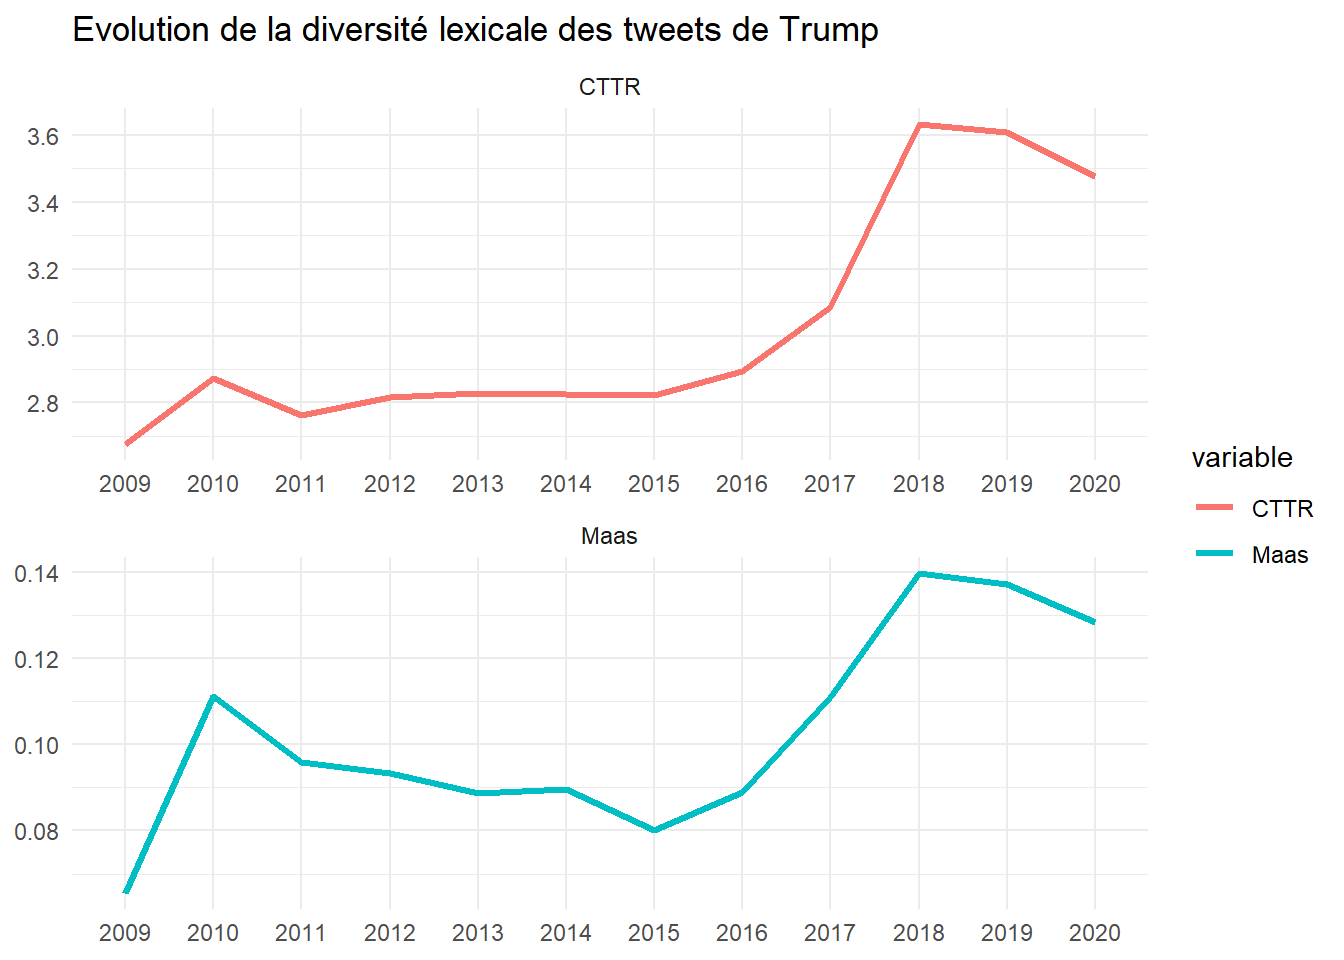
\includegraphics{q06_Analyse_quantitative_files/figure-pdf/610-1.pdf}

\section{La mesure de la concentration des
termes}\label{la-mesure-de-la-concentration-des-termes}

Le langage d'un point de vue quantitatif a été caractérisé depuis bien
longtemps et il est caractérisé par la loi de Zipf distribution 1949 .
Estout est un des premiers à avoir proposé la loi, mais un sténographe
fameux en aurait mis en évidence empiriquement avant 1916.

\subsection{Un débat théorique}\label{un-duxe9bat-thuxe9orique}

Celle-ci s'exprime de la manière suivante : si on classe les termes par
ordre de fréquence r, le produit de leur rang par la fréquence est égale
à une constante. Autrement dit dans une métrique log, la relation entre
rang et fréquence est linéaire et sa pente est négative.

\[f(r).{r}={K} \] Mandelbrot la généralise

les études empiriques

On peut encore débattre de sa signification. Une économie cognitive? Une
conséquence de la théorie de l'information ? Un signature pour
identifier un discours \#\# Les lois de distribution du langage

Les lois puissances qui déterminent cet univers et marque dans le
registre de l'analyse quantitative une évolution sérieuse. Alors que le
modèle dominant de la statistique est la distribution gaussienne, le
traitement du langage doit se familiariser avec des distributions
puissance.

La régularité statistique nécessite une interprétation, il n'y en a pas
qu'une

\begin{itemize}
\item
  la loi du moindre de effort qui va aboutir à un débat entre Mandelbrot
  et Simon.
\item
  Economie de l'information, un mot puis deux, puis trois, puis des mots
  spécifique à un certain registre d'action. Le sens est une affaire
  d'échelle, du concret au général. Le plus concret est celui des mots
  scientifiques telles qu'on les retrouve en biologie pour décrire une
  espèce, en droit pour décrire une propriété, ou en médecine pour
  désigner une pathologie ou un élément d'anatomie. ( espace de
  connaissance - épistémologique)
\item
  la distribution des locuteurs et de leurs élocution. Dans le langage
  vernaculaire celui de nos sociabilités, peu de mots sont employés, à
  mesure qu'on les enregistre ils prennent une place plus importance
  d'un point de de vue statistique dans les corpus. Les mots rares sont
  employés par peu de personne. (espace des population - démographique)
\end{itemize}

\subsection{Application}\label{application}

Examinons plus concrètement

On reprend la procédure de comptage des mots par groupe, mais sans
filtrer sur la fréquence de ces mots. On en obtient \texttt{n\_w} mots
distincts. En examinant avec plus de détail il y a 5 élément
d'information : a ) le trait (feature), c'est à dire ici le mot étudié,
b) le nombre de fois où il apparaît dans le corpus, c)le rank qui lui
correspond, d)le nombre de documents dans lesquels il apparaît.

Le tableau nous donne les 10 premiers. Il y a 28000 éléments, dont une
simple inspection montrera qu'il sont des liens ou d'autres mentions. Il
est nécessaire de retraiter le corpus pour éliminer ces éléments. Nous
étudierons comment faire dans les chapitres suivants. A ce stade on se
contente d'enlever les \emph{apax}\footnote{les apax sont les termes qui
  n'apparaissent qu'une seule fois dans un corpus.} dont on ne peut
véritablement calculer un rang ( ils ont tous le dernier). Il nous reste
10854 termes.

\begin{Shaded}
\begin{Highlighting}[]
\NormalTok{foo}\OtherTok{\textless{}{-}}\NormalTok{df }\SpecialCharTok{\%\textgreater{}\%} 
  \FunctionTok{filter}\NormalTok{(isRetweet}\SpecialCharTok{==}\ConstantTok{FALSE}\NormalTok{) }\SpecialCharTok{\%\textgreater{}\%}
  \FunctionTok{filter}\NormalTok{( Year }\SpecialCharTok{\%in\%} \FunctionTok{c}\NormalTok{(}\StringTok{"2016"}\NormalTok{,}\StringTok{"2017"}\NormalTok{,}\StringTok{"2018"}\NormalTok{,}\StringTok{"2019"}\NormalTok{,}\StringTok{"2020"}\NormalTok{))}\CommentTok{\# on ne prend pas en compte les RT}

\NormalTok{toks}\OtherTok{\textless{}{-}} \FunctionTok{tokens}\NormalTok{(foo}\SpecialCharTok{$}\NormalTok{text) }\SpecialCharTok{\%\textgreater{}\%} 
  \FunctionTok{dfm}\NormalTok{(}\AttributeTok{remove\_punct =} \ConstantTok{TRUE}\NormalTok{,  }\AttributeTok{remove =} \FunctionTok{stopwords}\NormalTok{(}\StringTok{"english"}\NormalTok{))}
\NormalTok{freq\_g }\OtherTok{\textless{}{-}} \FunctionTok{textstat\_frequency}\NormalTok{(toks)}\SpecialCharTok{\%\textgreater{}\%}
  \FunctionTok{as.data.frame}\NormalTok{() }\SpecialCharTok{\%\textgreater{}\%}
  \FunctionTok{filter}\NormalTok{(feature}\SpecialCharTok{!=}\StringTok{"amp"}\NormalTok{) }\SpecialCharTok{\%\textgreater{}\%}
  \FunctionTok{filter}\NormalTok{(frequency}\SpecialCharTok{\textgreater{}}\DecValTok{1}\NormalTok{)}

\FunctionTok{flextable}\NormalTok{(}\FunctionTok{head}\NormalTok{(freq\_g, }\DecValTok{15}\NormalTok{))}
\end{Highlighting}
\end{Shaded}

\global\setlength{\Oldarrayrulewidth}{\arrayrulewidth}

\global\setlength{\Oldtabcolsep}{\tabcolsep}

\setlength{\tabcolsep}{0pt}

\renewcommand*{\arraystretch}{1.5}



\providecommand{\ascline}[3]{\noalign{\global\arrayrulewidth #1}\arrayrulecolor[HTML]{#2}\cline{#3}}

\begin{longtable}[c]{|p{0.75in}|p{0.75in}|p{0.75in}|p{0.75in}|p{0.75in}}
\caption{Mots les plus fréquents}\tabularnewline




\hhline{>{\arrayrulecolor[HTML]{666666}\global\arrayrulewidth=1.5pt}->{\arrayrulecolor[HTML]{666666}\global\arrayrulewidth=1.5pt}->{\arrayrulecolor[HTML]{666666}\global\arrayrulewidth=1.5pt}->{\arrayrulecolor[HTML]{666666}\global\arrayrulewidth=1.5pt}->{\arrayrulecolor[HTML]{666666}\global\arrayrulewidth=1.5pt}-}

\multicolumn{1}{>{\cellcolor[HTML]{EFEFEF}\raggedright}m{\dimexpr 0.75in+0\tabcolsep}}{\textcolor[HTML]{000000}{\fontsize{10}{10}\selectfont{\textbf{feature}}}} & \multicolumn{1}{>{\cellcolor[HTML]{EFEFEF}\raggedleft}m{\dimexpr 0.75in+0\tabcolsep}}{\textcolor[HTML]{000000}{\fontsize{10}{10}\selectfont{\textbf{frequency}}}} & \multicolumn{1}{>{\cellcolor[HTML]{EFEFEF}\raggedleft}m{\dimexpr 0.75in+0\tabcolsep}}{\textcolor[HTML]{000000}{\fontsize{10}{10}\selectfont{\textbf{rank}}}} & \multicolumn{1}{>{\cellcolor[HTML]{EFEFEF}\raggedleft}m{\dimexpr 0.75in+0\tabcolsep}}{\textcolor[HTML]{000000}{\fontsize{10}{10}\selectfont{\textbf{docfreq}}}} & \multicolumn{1}{>{\cellcolor[HTML]{EFEFEF}\raggedright}m{\dimexpr 0.75in+0\tabcolsep}}{\textcolor[HTML]{000000}{\fontsize{10}{10}\selectfont{\textbf{group}}}} \\

\noalign{\global\arrayrulewidth 0pt}\arrayrulecolor[HTML]{000000}

\hhline{>{\arrayrulecolor[HTML]{666666}\global\arrayrulewidth=1.5pt}->{\arrayrulecolor[HTML]{666666}\global\arrayrulewidth=1.5pt}->{\arrayrulecolor[HTML]{666666}\global\arrayrulewidth=1.5pt}->{\arrayrulecolor[HTML]{666666}\global\arrayrulewidth=1.5pt}->{\arrayrulecolor[HTML]{666666}\global\arrayrulewidth=1.5pt}-}\endfirsthead 

\hhline{>{\arrayrulecolor[HTML]{666666}\global\arrayrulewidth=1.5pt}->{\arrayrulecolor[HTML]{666666}\global\arrayrulewidth=1.5pt}->{\arrayrulecolor[HTML]{666666}\global\arrayrulewidth=1.5pt}->{\arrayrulecolor[HTML]{666666}\global\arrayrulewidth=1.5pt}->{\arrayrulecolor[HTML]{666666}\global\arrayrulewidth=1.5pt}-}

\multicolumn{1}{>{\cellcolor[HTML]{EFEFEF}\raggedright}m{\dimexpr 0.75in+0\tabcolsep}}{\textcolor[HTML]{000000}{\fontsize{10}{10}\selectfont{\textbf{feature}}}} & \multicolumn{1}{>{\cellcolor[HTML]{EFEFEF}\raggedleft}m{\dimexpr 0.75in+0\tabcolsep}}{\textcolor[HTML]{000000}{\fontsize{10}{10}\selectfont{\textbf{frequency}}}} & \multicolumn{1}{>{\cellcolor[HTML]{EFEFEF}\raggedleft}m{\dimexpr 0.75in+0\tabcolsep}}{\textcolor[HTML]{000000}{\fontsize{10}{10}\selectfont{\textbf{rank}}}} & \multicolumn{1}{>{\cellcolor[HTML]{EFEFEF}\raggedleft}m{\dimexpr 0.75in+0\tabcolsep}}{\textcolor[HTML]{000000}{\fontsize{10}{10}\selectfont{\textbf{docfreq}}}} & \multicolumn{1}{>{\cellcolor[HTML]{EFEFEF}\raggedright}m{\dimexpr 0.75in+0\tabcolsep}}{\textcolor[HTML]{000000}{\fontsize{10}{10}\selectfont{\textbf{group}}}} \\

\noalign{\global\arrayrulewidth 0pt}\arrayrulecolor[HTML]{000000}

\hhline{>{\arrayrulecolor[HTML]{666666}\global\arrayrulewidth=1.5pt}->{\arrayrulecolor[HTML]{666666}\global\arrayrulewidth=1.5pt}->{\arrayrulecolor[HTML]{666666}\global\arrayrulewidth=1.5pt}->{\arrayrulecolor[HTML]{666666}\global\arrayrulewidth=1.5pt}->{\arrayrulecolor[HTML]{666666}\global\arrayrulewidth=1.5pt}-}\endhead



\multicolumn{1}{>{\cellcolor[HTML]{EFEFEF}\raggedright}m{\dimexpr 0.75in+0\tabcolsep}}{\textcolor[HTML]{000000}{\fontsize{10}{10}\selectfont{great}}} & \multicolumn{1}{>{\cellcolor[HTML]{EFEFEF}\raggedleft}m{\dimexpr 0.75in+0\tabcolsep}}{\textcolor[HTML]{000000}{\fontsize{10}{10}\selectfont{4,077}}} & \multicolumn{1}{>{\cellcolor[HTML]{EFEFEF}\raggedleft}m{\dimexpr 0.75in+0\tabcolsep}}{\textcolor[HTML]{000000}{\fontsize{10}{10}\selectfont{1}}} & \multicolumn{1}{>{\cellcolor[HTML]{EFEFEF}\raggedleft}m{\dimexpr 0.75in+0\tabcolsep}}{\textcolor[HTML]{000000}{\fontsize{10}{10}\selectfont{3,755}}} & \multicolumn{1}{>{\cellcolor[HTML]{EFEFEF}\raggedright}m{\dimexpr 0.75in+0\tabcolsep}}{\textcolor[HTML]{000000}{\fontsize{10}{10}\selectfont{all}}} \\

\noalign{\global\arrayrulewidth 0pt}\arrayrulecolor[HTML]{000000}

\hhline{>{\arrayrulecolor[HTML]{666666}\global\arrayrulewidth=0.75pt}->{\arrayrulecolor[HTML]{666666}\global\arrayrulewidth=0.75pt}->{\arrayrulecolor[HTML]{666666}\global\arrayrulewidth=0.75pt}->{\arrayrulecolor[HTML]{666666}\global\arrayrulewidth=0.75pt}->{\arrayrulecolor[HTML]{666666}\global\arrayrulewidth=0.75pt}-}



\multicolumn{1}{>{\cellcolor[HTML]{EFEFEF}\raggedright}m{\dimexpr 0.75in+0\tabcolsep}}{\textcolor[HTML]{000000}{\fontsize{10}{10}\selectfont{thank}}} & \multicolumn{1}{>{\cellcolor[HTML]{EFEFEF}\raggedleft}m{\dimexpr 0.75in+0\tabcolsep}}{\textcolor[HTML]{000000}{\fontsize{10}{10}\selectfont{2,041}}} & \multicolumn{1}{>{\cellcolor[HTML]{EFEFEF}\raggedleft}m{\dimexpr 0.75in+0\tabcolsep}}{\textcolor[HTML]{000000}{\fontsize{10}{10}\selectfont{3}}} & \multicolumn{1}{>{\cellcolor[HTML]{EFEFEF}\raggedleft}m{\dimexpr 0.75in+0\tabcolsep}}{\textcolor[HTML]{000000}{\fontsize{10}{10}\selectfont{2,029}}} & \multicolumn{1}{>{\cellcolor[HTML]{EFEFEF}\raggedright}m{\dimexpr 0.75in+0\tabcolsep}}{\textcolor[HTML]{000000}{\fontsize{10}{10}\selectfont{all}}} \\

\noalign{\global\arrayrulewidth 0pt}\arrayrulecolor[HTML]{000000}

\hhline{>{\arrayrulecolor[HTML]{666666}\global\arrayrulewidth=0.75pt}->{\arrayrulecolor[HTML]{666666}\global\arrayrulewidth=0.75pt}->{\arrayrulecolor[HTML]{666666}\global\arrayrulewidth=0.75pt}->{\arrayrulecolor[HTML]{666666}\global\arrayrulewidth=0.75pt}->{\arrayrulecolor[HTML]{666666}\global\arrayrulewidth=0.75pt}-}



\multicolumn{1}{>{\cellcolor[HTML]{EFEFEF}\raggedright}m{\dimexpr 0.75in+0\tabcolsep}}{\textcolor[HTML]{000000}{\fontsize{10}{10}\selectfont{people}}} & \multicolumn{1}{>{\cellcolor[HTML]{EFEFEF}\raggedleft}m{\dimexpr 0.75in+0\tabcolsep}}{\textcolor[HTML]{000000}{\fontsize{10}{10}\selectfont{2,040}}} & \multicolumn{1}{>{\cellcolor[HTML]{EFEFEF}\raggedleft}m{\dimexpr 0.75in+0\tabcolsep}}{\textcolor[HTML]{000000}{\fontsize{10}{10}\selectfont{4}}} & \multicolumn{1}{>{\cellcolor[HTML]{EFEFEF}\raggedleft}m{\dimexpr 0.75in+0\tabcolsep}}{\textcolor[HTML]{000000}{\fontsize{10}{10}\selectfont{1,895}}} & \multicolumn{1}{>{\cellcolor[HTML]{EFEFEF}\raggedright}m{\dimexpr 0.75in+0\tabcolsep}}{\textcolor[HTML]{000000}{\fontsize{10}{10}\selectfont{all}}} \\

\noalign{\global\arrayrulewidth 0pt}\arrayrulecolor[HTML]{000000}

\hhline{>{\arrayrulecolor[HTML]{666666}\global\arrayrulewidth=0.75pt}->{\arrayrulecolor[HTML]{666666}\global\arrayrulewidth=0.75pt}->{\arrayrulecolor[HTML]{666666}\global\arrayrulewidth=0.75pt}->{\arrayrulecolor[HTML]{666666}\global\arrayrulewidth=0.75pt}->{\arrayrulecolor[HTML]{666666}\global\arrayrulewidth=0.75pt}-}



\multicolumn{1}{>{\cellcolor[HTML]{EFEFEF}\raggedright}m{\dimexpr 0.75in+0\tabcolsep}}{\textcolor[HTML]{000000}{\fontsize{10}{10}\selectfont{just}}} & \multicolumn{1}{>{\cellcolor[HTML]{EFEFEF}\raggedleft}m{\dimexpr 0.75in+0\tabcolsep}}{\textcolor[HTML]{000000}{\fontsize{10}{10}\selectfont{1,633}}} & \multicolumn{1}{>{\cellcolor[HTML]{EFEFEF}\raggedleft}m{\dimexpr 0.75in+0\tabcolsep}}{\textcolor[HTML]{000000}{\fontsize{10}{10}\selectfont{5}}} & \multicolumn{1}{>{\cellcolor[HTML]{EFEFEF}\raggedleft}m{\dimexpr 0.75in+0\tabcolsep}}{\textcolor[HTML]{000000}{\fontsize{10}{10}\selectfont{1,572}}} & \multicolumn{1}{>{\cellcolor[HTML]{EFEFEF}\raggedright}m{\dimexpr 0.75in+0\tabcolsep}}{\textcolor[HTML]{000000}{\fontsize{10}{10}\selectfont{all}}} \\

\noalign{\global\arrayrulewidth 0pt}\arrayrulecolor[HTML]{000000}

\hhline{>{\arrayrulecolor[HTML]{666666}\global\arrayrulewidth=0.75pt}->{\arrayrulecolor[HTML]{666666}\global\arrayrulewidth=0.75pt}->{\arrayrulecolor[HTML]{666666}\global\arrayrulewidth=0.75pt}->{\arrayrulecolor[HTML]{666666}\global\arrayrulewidth=0.75pt}->{\arrayrulecolor[HTML]{666666}\global\arrayrulewidth=0.75pt}-}



\multicolumn{1}{>{\cellcolor[HTML]{EFEFEF}\raggedright}m{\dimexpr 0.75in+0\tabcolsep}}{\textcolor[HTML]{000000}{\fontsize{10}{10}\selectfont{now}}} & \multicolumn{1}{>{\cellcolor[HTML]{EFEFEF}\raggedleft}m{\dimexpr 0.75in+0\tabcolsep}}{\textcolor[HTML]{000000}{\fontsize{10}{10}\selectfont{1,544}}} & \multicolumn{1}{>{\cellcolor[HTML]{EFEFEF}\raggedleft}m{\dimexpr 0.75in+0\tabcolsep}}{\textcolor[HTML]{000000}{\fontsize{10}{10}\selectfont{6}}} & \multicolumn{1}{>{\cellcolor[HTML]{EFEFEF}\raggedleft}m{\dimexpr 0.75in+0\tabcolsep}}{\textcolor[HTML]{000000}{\fontsize{10}{10}\selectfont{1,505}}} & \multicolumn{1}{>{\cellcolor[HTML]{EFEFEF}\raggedright}m{\dimexpr 0.75in+0\tabcolsep}}{\textcolor[HTML]{000000}{\fontsize{10}{10}\selectfont{all}}} \\

\noalign{\global\arrayrulewidth 0pt}\arrayrulecolor[HTML]{000000}

\hhline{>{\arrayrulecolor[HTML]{666666}\global\arrayrulewidth=0.75pt}->{\arrayrulecolor[HTML]{666666}\global\arrayrulewidth=0.75pt}->{\arrayrulecolor[HTML]{666666}\global\arrayrulewidth=0.75pt}->{\arrayrulecolor[HTML]{666666}\global\arrayrulewidth=0.75pt}->{\arrayrulecolor[HTML]{666666}\global\arrayrulewidth=0.75pt}-}



\multicolumn{1}{>{\cellcolor[HTML]{EFEFEF}\raggedright}m{\dimexpr 0.75in+0\tabcolsep}}{\textcolor[HTML]{000000}{\fontsize{10}{10}\selectfont{president}}} & \multicolumn{1}{>{\cellcolor[HTML]{EFEFEF}\raggedleft}m{\dimexpr 0.75in+0\tabcolsep}}{\textcolor[HTML]{000000}{\fontsize{10}{10}\selectfont{1,466}}} & \multicolumn{1}{>{\cellcolor[HTML]{EFEFEF}\raggedleft}m{\dimexpr 0.75in+0\tabcolsep}}{\textcolor[HTML]{000000}{\fontsize{10}{10}\selectfont{7}}} & \multicolumn{1}{>{\cellcolor[HTML]{EFEFEF}\raggedleft}m{\dimexpr 0.75in+0\tabcolsep}}{\textcolor[HTML]{000000}{\fontsize{10}{10}\selectfont{1,322}}} & \multicolumn{1}{>{\cellcolor[HTML]{EFEFEF}\raggedright}m{\dimexpr 0.75in+0\tabcolsep}}{\textcolor[HTML]{000000}{\fontsize{10}{10}\selectfont{all}}} \\

\noalign{\global\arrayrulewidth 0pt}\arrayrulecolor[HTML]{000000}

\hhline{>{\arrayrulecolor[HTML]{666666}\global\arrayrulewidth=0.75pt}->{\arrayrulecolor[HTML]{666666}\global\arrayrulewidth=0.75pt}->{\arrayrulecolor[HTML]{666666}\global\arrayrulewidth=0.75pt}->{\arrayrulecolor[HTML]{666666}\global\arrayrulewidth=0.75pt}->{\arrayrulecolor[HTML]{666666}\global\arrayrulewidth=0.75pt}-}



\multicolumn{1}{>{\cellcolor[HTML]{EFEFEF}\raggedright}m{\dimexpr 0.75in+0\tabcolsep}}{\textcolor[HTML]{000000}{\fontsize{10}{10}\selectfont{trump}}} & \multicolumn{1}{>{\cellcolor[HTML]{EFEFEF}\raggedleft}m{\dimexpr 0.75in+0\tabcolsep}}{\textcolor[HTML]{000000}{\fontsize{10}{10}\selectfont{1,424}}} & \multicolumn{1}{>{\cellcolor[HTML]{EFEFEF}\raggedleft}m{\dimexpr 0.75in+0\tabcolsep}}{\textcolor[HTML]{000000}{\fontsize{10}{10}\selectfont{8}}} & \multicolumn{1}{>{\cellcolor[HTML]{EFEFEF}\raggedleft}m{\dimexpr 0.75in+0\tabcolsep}}{\textcolor[HTML]{000000}{\fontsize{10}{10}\selectfont{1,307}}} & \multicolumn{1}{>{\cellcolor[HTML]{EFEFEF}\raggedright}m{\dimexpr 0.75in+0\tabcolsep}}{\textcolor[HTML]{000000}{\fontsize{10}{10}\selectfont{all}}} \\

\noalign{\global\arrayrulewidth 0pt}\arrayrulecolor[HTML]{000000}

\hhline{>{\arrayrulecolor[HTML]{666666}\global\arrayrulewidth=0.75pt}->{\arrayrulecolor[HTML]{666666}\global\arrayrulewidth=0.75pt}->{\arrayrulecolor[HTML]{666666}\global\arrayrulewidth=0.75pt}->{\arrayrulecolor[HTML]{666666}\global\arrayrulewidth=0.75pt}->{\arrayrulecolor[HTML]{666666}\global\arrayrulewidth=0.75pt}-}



\multicolumn{1}{>{\cellcolor[HTML]{EFEFEF}\raggedright}m{\dimexpr 0.75in+0\tabcolsep}}{\textcolor[HTML]{000000}{\fontsize{10}{10}\selectfont{big}}} & \multicolumn{1}{>{\cellcolor[HTML]{EFEFEF}\raggedleft}m{\dimexpr 0.75in+0\tabcolsep}}{\textcolor[HTML]{000000}{\fontsize{10}{10}\selectfont{1,360}}} & \multicolumn{1}{>{\cellcolor[HTML]{EFEFEF}\raggedleft}m{\dimexpr 0.75in+0\tabcolsep}}{\textcolor[HTML]{000000}{\fontsize{10}{10}\selectfont{9}}} & \multicolumn{1}{>{\cellcolor[HTML]{EFEFEF}\raggedleft}m{\dimexpr 0.75in+0\tabcolsep}}{\textcolor[HTML]{000000}{\fontsize{10}{10}\selectfont{1,263}}} & \multicolumn{1}{>{\cellcolor[HTML]{EFEFEF}\raggedright}m{\dimexpr 0.75in+0\tabcolsep}}{\textcolor[HTML]{000000}{\fontsize{10}{10}\selectfont{all}}} \\

\noalign{\global\arrayrulewidth 0pt}\arrayrulecolor[HTML]{000000}

\hhline{>{\arrayrulecolor[HTML]{666666}\global\arrayrulewidth=0.75pt}->{\arrayrulecolor[HTML]{666666}\global\arrayrulewidth=0.75pt}->{\arrayrulecolor[HTML]{666666}\global\arrayrulewidth=0.75pt}->{\arrayrulecolor[HTML]{666666}\global\arrayrulewidth=0.75pt}->{\arrayrulecolor[HTML]{666666}\global\arrayrulewidth=0.75pt}-}



\multicolumn{1}{>{\cellcolor[HTML]{EFEFEF}\raggedright}m{\dimexpr 0.75in+0\tabcolsep}}{\textcolor[HTML]{000000}{\fontsize{10}{10}\selectfont{news}}} & \multicolumn{1}{>{\cellcolor[HTML]{EFEFEF}\raggedleft}m{\dimexpr 0.75in+0\tabcolsep}}{\textcolor[HTML]{000000}{\fontsize{10}{10}\selectfont{1,347}}} & \multicolumn{1}{>{\cellcolor[HTML]{EFEFEF}\raggedleft}m{\dimexpr 0.75in+0\tabcolsep}}{\textcolor[HTML]{000000}{\fontsize{10}{10}\selectfont{10}}} & \multicolumn{1}{>{\cellcolor[HTML]{EFEFEF}\raggedleft}m{\dimexpr 0.75in+0\tabcolsep}}{\textcolor[HTML]{000000}{\fontsize{10}{10}\selectfont{1,254}}} & \multicolumn{1}{>{\cellcolor[HTML]{EFEFEF}\raggedright}m{\dimexpr 0.75in+0\tabcolsep}}{\textcolor[HTML]{000000}{\fontsize{10}{10}\selectfont{all}}} \\

\noalign{\global\arrayrulewidth 0pt}\arrayrulecolor[HTML]{000000}

\hhline{>{\arrayrulecolor[HTML]{666666}\global\arrayrulewidth=0.75pt}->{\arrayrulecolor[HTML]{666666}\global\arrayrulewidth=0.75pt}->{\arrayrulecolor[HTML]{666666}\global\arrayrulewidth=0.75pt}->{\arrayrulecolor[HTML]{666666}\global\arrayrulewidth=0.75pt}->{\arrayrulecolor[HTML]{666666}\global\arrayrulewidth=0.75pt}-}



\multicolumn{1}{>{\cellcolor[HTML]{EFEFEF}\raggedright}m{\dimexpr 0.75in+0\tabcolsep}}{\textcolor[HTML]{000000}{\fontsize{10}{10}\selectfont{country}}} & \multicolumn{1}{>{\cellcolor[HTML]{EFEFEF}\raggedleft}m{\dimexpr 0.75in+0\tabcolsep}}{\textcolor[HTML]{000000}{\fontsize{10}{10}\selectfont{1,274}}} & \multicolumn{1}{>{\cellcolor[HTML]{EFEFEF}\raggedleft}m{\dimexpr 0.75in+0\tabcolsep}}{\textcolor[HTML]{000000}{\fontsize{10}{10}\selectfont{11}}} & \multicolumn{1}{>{\cellcolor[HTML]{EFEFEF}\raggedleft}m{\dimexpr 0.75in+0\tabcolsep}}{\textcolor[HTML]{000000}{\fontsize{10}{10}\selectfont{1,233}}} & \multicolumn{1}{>{\cellcolor[HTML]{EFEFEF}\raggedright}m{\dimexpr 0.75in+0\tabcolsep}}{\textcolor[HTML]{000000}{\fontsize{10}{10}\selectfont{all}}} \\

\noalign{\global\arrayrulewidth 0pt}\arrayrulecolor[HTML]{000000}

\hhline{>{\arrayrulecolor[HTML]{666666}\global\arrayrulewidth=0.75pt}->{\arrayrulecolor[HTML]{666666}\global\arrayrulewidth=0.75pt}->{\arrayrulecolor[HTML]{666666}\global\arrayrulewidth=0.75pt}->{\arrayrulecolor[HTML]{666666}\global\arrayrulewidth=0.75pt}->{\arrayrulecolor[HTML]{666666}\global\arrayrulewidth=0.75pt}-}



\multicolumn{1}{>{\cellcolor[HTML]{EFEFEF}\raggedright}m{\dimexpr 0.75in+0\tabcolsep}}{\textcolor[HTML]{000000}{\fontsize{10}{10}\selectfont{get}}} & \multicolumn{1}{>{\cellcolor[HTML]{EFEFEF}\raggedleft}m{\dimexpr 0.75in+0\tabcolsep}}{\textcolor[HTML]{000000}{\fontsize{10}{10}\selectfont{1,180}}} & \multicolumn{1}{>{\cellcolor[HTML]{EFEFEF}\raggedleft}m{\dimexpr 0.75in+0\tabcolsep}}{\textcolor[HTML]{000000}{\fontsize{10}{10}\selectfont{12}}} & \multicolumn{1}{>{\cellcolor[HTML]{EFEFEF}\raggedleft}m{\dimexpr 0.75in+0\tabcolsep}}{\textcolor[HTML]{000000}{\fontsize{10}{10}\selectfont{1,083}}} & \multicolumn{1}{>{\cellcolor[HTML]{EFEFEF}\raggedright}m{\dimexpr 0.75in+0\tabcolsep}}{\textcolor[HTML]{000000}{\fontsize{10}{10}\selectfont{all}}} \\

\noalign{\global\arrayrulewidth 0pt}\arrayrulecolor[HTML]{000000}

\hhline{>{\arrayrulecolor[HTML]{666666}\global\arrayrulewidth=0.75pt}->{\arrayrulecolor[HTML]{666666}\global\arrayrulewidth=0.75pt}->{\arrayrulecolor[HTML]{666666}\global\arrayrulewidth=0.75pt}->{\arrayrulecolor[HTML]{666666}\global\arrayrulewidth=0.75pt}->{\arrayrulecolor[HTML]{666666}\global\arrayrulewidth=0.75pt}-}



\multicolumn{1}{>{\cellcolor[HTML]{EFEFEF}\raggedright}m{\dimexpr 0.75in+0\tabcolsep}}{\textcolor[HTML]{000000}{\fontsize{10}{10}\selectfont{fake}}} & \multicolumn{1}{>{\cellcolor[HTML]{EFEFEF}\raggedleft}m{\dimexpr 0.75in+0\tabcolsep}}{\textcolor[HTML]{000000}{\fontsize{10}{10}\selectfont{1,177}}} & \multicolumn{1}{>{\cellcolor[HTML]{EFEFEF}\raggedleft}m{\dimexpr 0.75in+0\tabcolsep}}{\textcolor[HTML]{000000}{\fontsize{10}{10}\selectfont{13}}} & \multicolumn{1}{>{\cellcolor[HTML]{EFEFEF}\raggedleft}m{\dimexpr 0.75in+0\tabcolsep}}{\textcolor[HTML]{000000}{\fontsize{10}{10}\selectfont{1,100}}} & \multicolumn{1}{>{\cellcolor[HTML]{EFEFEF}\raggedright}m{\dimexpr 0.75in+0\tabcolsep}}{\textcolor[HTML]{000000}{\fontsize{10}{10}\selectfont{all}}} \\

\noalign{\global\arrayrulewidth 0pt}\arrayrulecolor[HTML]{000000}

\hhline{>{\arrayrulecolor[HTML]{666666}\global\arrayrulewidth=0.75pt}->{\arrayrulecolor[HTML]{666666}\global\arrayrulewidth=0.75pt}->{\arrayrulecolor[HTML]{666666}\global\arrayrulewidth=0.75pt}->{\arrayrulecolor[HTML]{666666}\global\arrayrulewidth=0.75pt}->{\arrayrulecolor[HTML]{666666}\global\arrayrulewidth=0.75pt}-}



\multicolumn{1}{>{\cellcolor[HTML]{EFEFEF}\raggedright}m{\dimexpr 0.75in+0\tabcolsep}}{\textcolor[HTML]{000000}{\fontsize{10}{10}\selectfont{new}}} & \multicolumn{1}{>{\cellcolor[HTML]{EFEFEF}\raggedleft}m{\dimexpr 0.75in+0\tabcolsep}}{\textcolor[HTML]{000000}{\fontsize{10}{10}\selectfont{1,167}}} & \multicolumn{1}{>{\cellcolor[HTML]{EFEFEF}\raggedleft}m{\dimexpr 0.75in+0\tabcolsep}}{\textcolor[HTML]{000000}{\fontsize{10}{10}\selectfont{14}}} & \multicolumn{1}{>{\cellcolor[HTML]{EFEFEF}\raggedleft}m{\dimexpr 0.75in+0\tabcolsep}}{\textcolor[HTML]{000000}{\fontsize{10}{10}\selectfont{1,089}}} & \multicolumn{1}{>{\cellcolor[HTML]{EFEFEF}\raggedright}m{\dimexpr 0.75in+0\tabcolsep}}{\textcolor[HTML]{000000}{\fontsize{10}{10}\selectfont{all}}} \\

\noalign{\global\arrayrulewidth 0pt}\arrayrulecolor[HTML]{000000}

\hhline{>{\arrayrulecolor[HTML]{666666}\global\arrayrulewidth=0.75pt}->{\arrayrulecolor[HTML]{666666}\global\arrayrulewidth=0.75pt}->{\arrayrulecolor[HTML]{666666}\global\arrayrulewidth=0.75pt}->{\arrayrulecolor[HTML]{666666}\global\arrayrulewidth=0.75pt}->{\arrayrulecolor[HTML]{666666}\global\arrayrulewidth=0.75pt}-}



\multicolumn{1}{>{\cellcolor[HTML]{EFEFEF}\raggedright}m{\dimexpr 0.75in+0\tabcolsep}}{\textcolor[HTML]{000000}{\fontsize{10}{10}\selectfont{democrats}}} & \multicolumn{1}{>{\cellcolor[HTML]{EFEFEF}\raggedleft}m{\dimexpr 0.75in+0\tabcolsep}}{\textcolor[HTML]{000000}{\fontsize{10}{10}\selectfont{1,163}}} & \multicolumn{1}{>{\cellcolor[HTML]{EFEFEF}\raggedleft}m{\dimexpr 0.75in+0\tabcolsep}}{\textcolor[HTML]{000000}{\fontsize{10}{10}\selectfont{15}}} & \multicolumn{1}{>{\cellcolor[HTML]{EFEFEF}\raggedleft}m{\dimexpr 0.75in+0\tabcolsep}}{\textcolor[HTML]{000000}{\fontsize{10}{10}\selectfont{1,119}}} & \multicolumn{1}{>{\cellcolor[HTML]{EFEFEF}\raggedright}m{\dimexpr 0.75in+0\tabcolsep}}{\textcolor[HTML]{000000}{\fontsize{10}{10}\selectfont{all}}} \\

\noalign{\global\arrayrulewidth 0pt}\arrayrulecolor[HTML]{000000}

\hhline{>{\arrayrulecolor[HTML]{666666}\global\arrayrulewidth=0.75pt}->{\arrayrulecolor[HTML]{666666}\global\arrayrulewidth=0.75pt}->{\arrayrulecolor[HTML]{666666}\global\arrayrulewidth=0.75pt}->{\arrayrulecolor[HTML]{666666}\global\arrayrulewidth=0.75pt}->{\arrayrulecolor[HTML]{666666}\global\arrayrulewidth=0.75pt}-}



\multicolumn{1}{>{\cellcolor[HTML]{EFEFEF}\raggedright}m{\dimexpr 0.75in+0\tabcolsep}}{\textcolor[HTML]{000000}{\fontsize{10}{10}\selectfont{many}}} & \multicolumn{1}{>{\cellcolor[HTML]{EFEFEF}\raggedleft}m{\dimexpr 0.75in+0\tabcolsep}}{\textcolor[HTML]{000000}{\fontsize{10}{10}\selectfont{1,108}}} & \multicolumn{1}{>{\cellcolor[HTML]{EFEFEF}\raggedleft}m{\dimexpr 0.75in+0\tabcolsep}}{\textcolor[HTML]{000000}{\fontsize{10}{10}\selectfont{16}}} & \multicolumn{1}{>{\cellcolor[HTML]{EFEFEF}\raggedleft}m{\dimexpr 0.75in+0\tabcolsep}}{\textcolor[HTML]{000000}{\fontsize{10}{10}\selectfont{1,061}}} & \multicolumn{1}{>{\cellcolor[HTML]{EFEFEF}\raggedright}m{\dimexpr 0.75in+0\tabcolsep}}{\textcolor[HTML]{000000}{\fontsize{10}{10}\selectfont{all}}} \\

\noalign{\global\arrayrulewidth 0pt}\arrayrulecolor[HTML]{000000}

\hhline{>{\arrayrulecolor[HTML]{666666}\global\arrayrulewidth=1.5pt}->{\arrayrulecolor[HTML]{666666}\global\arrayrulewidth=1.5pt}->{\arrayrulecolor[HTML]{666666}\global\arrayrulewidth=1.5pt}->{\arrayrulecolor[HTML]{666666}\global\arrayrulewidth=1.5pt}->{\arrayrulecolor[HTML]{666666}\global\arrayrulewidth=1.5pt}-}



\end{longtable}



\arrayrulecolor[HTML]{000000}

\global\setlength{\arrayrulewidth}{\Oldarrayrulewidth}

\global\setlength{\tabcolsep}{\Oldtabcolsep}

\renewcommand*{\arraystretch}{1}

On peut aussi représenter cela graphiquement. La loi de zipf s'observe
jusqu'au 500 premiers mots, ensuite elle suit une autre pente. C'est
assez caractéristique, la loi de zipf est incomplète, d'un point de vue
empirique il semble qu'il y ait deux lois qui se superposes, la loi des
mots communs, et celle des mots singuliers. C'est du moins hypothèse que
nous proposons.

\begin{Shaded}
\begin{Highlighting}[]
\FunctionTok{ggplot}\NormalTok{(freq\_g, }\FunctionTok{aes}\NormalTok{(}\AttributeTok{x=}\NormalTok{rank, }\AttributeTok{y=}\NormalTok{frequency))}\SpecialCharTok{+}
  \FunctionTok{geom\_point}\NormalTok{(}\AttributeTok{size=}\NormalTok{.}\DecValTok{1}\NormalTok{)}\SpecialCharTok{+}
  \FunctionTok{scale\_x\_log10}\NormalTok{()}\SpecialCharTok{+}
  \FunctionTok{scale\_y\_log10}\NormalTok{() }\SpecialCharTok{+} 
  \FunctionTok{geom\_smooth}\NormalTok{(}\AttributeTok{method=}\StringTok{"gam"}\NormalTok{, }\AttributeTok{color=}\NormalTok{col\_1)}
\end{Highlighting}
\end{Shaded}

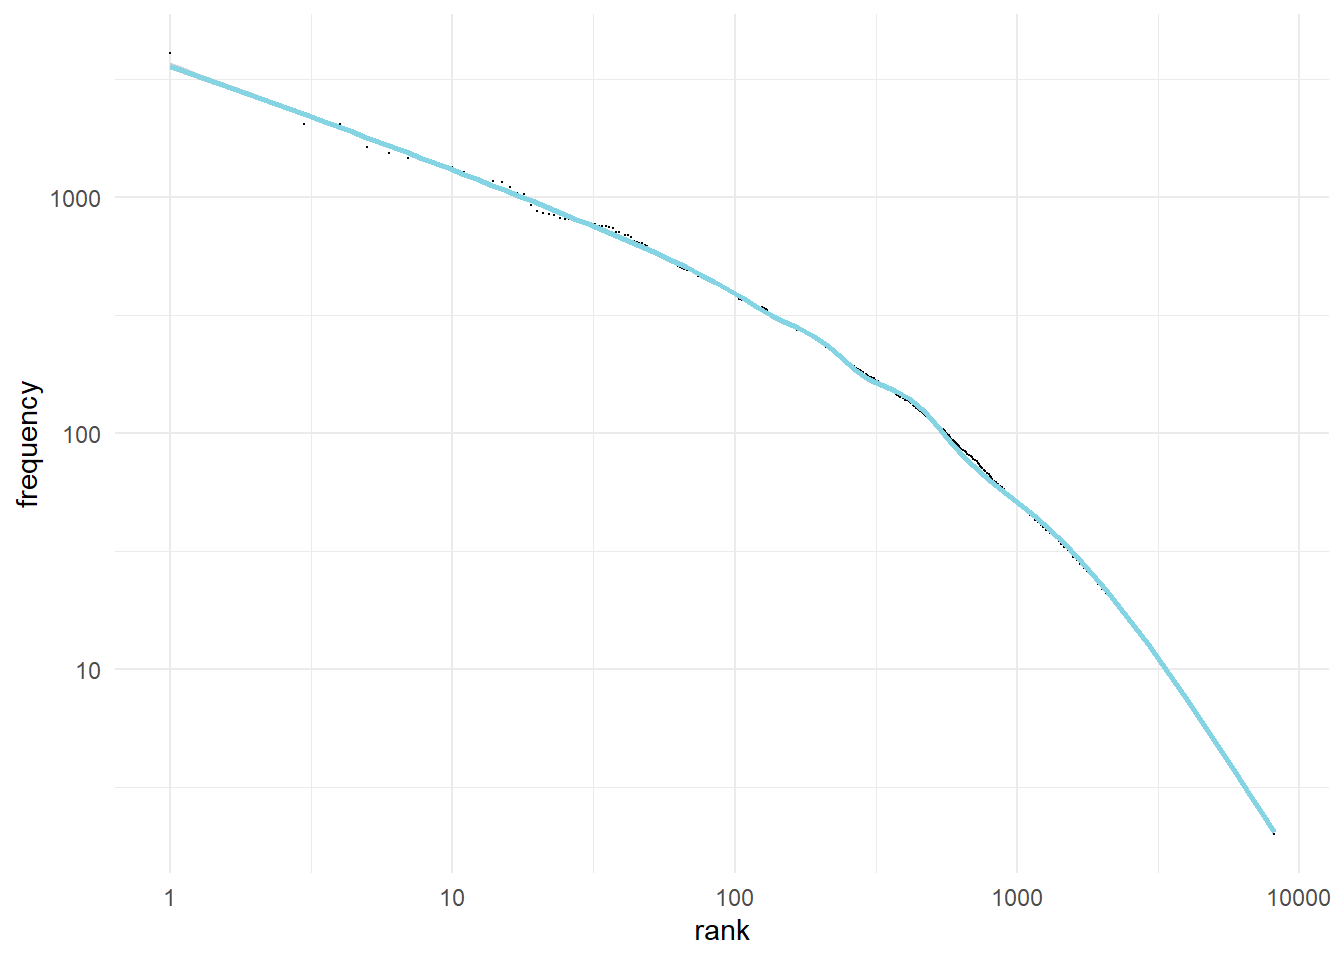
\includegraphics{q06_Analyse_quantitative_files/figure-pdf/612-1.pdf}

\begin{Shaded}
\begin{Highlighting}[]
\NormalTok{foo}\OtherTok{\textless{}{-}}\NormalTok{freq\_g }\SpecialCharTok{\%\textgreater{}\%}\FunctionTok{filter}\NormalTok{(rank }\SpecialCharTok{\textless{}}\DecValTok{500}\NormalTok{)}
\FunctionTok{ggplot}\NormalTok{(foo, }\FunctionTok{aes}\NormalTok{(}\AttributeTok{x=}\NormalTok{rank, }\AttributeTok{y=}\NormalTok{frequency))}\SpecialCharTok{+}
  \FunctionTok{geom\_point}\NormalTok{(}\AttributeTok{size=}\NormalTok{.}\DecValTok{1}\NormalTok{)}\SpecialCharTok{+}
  \FunctionTok{scale\_x\_log10}\NormalTok{()}\SpecialCharTok{+}
  \FunctionTok{scale\_y\_log10}\NormalTok{() }\SpecialCharTok{+} 
  \FunctionTok{geom\_smooth}\NormalTok{(}\AttributeTok{method=}\StringTok{"lm"}\NormalTok{, }\AttributeTok{color=}\NormalTok{col\_1)}
\end{Highlighting}
\end{Shaded}

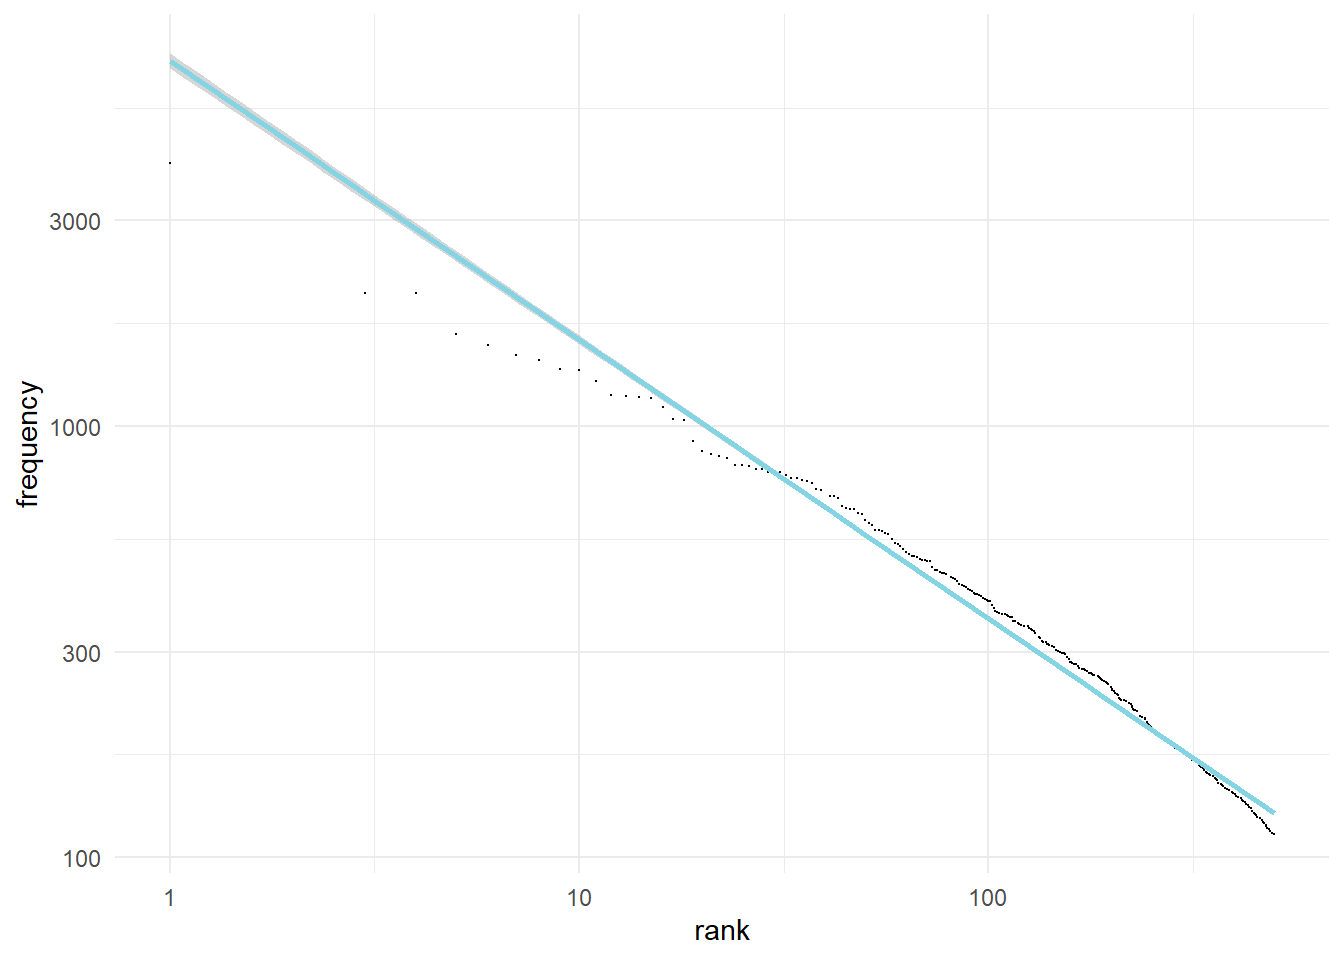
\includegraphics{q06_Analyse_quantitative_files/figure-pdf/612-2.pdf}

Pour être plus qualitatif Une première manière de représenter la
diversité du corpus est de représenter les mots les plus fréquents,
selon cette fréquente et le ratio fréquence par document. Plus ce
dernier est élevé plus il fait du mot un mot spécifique.

\begin{Shaded}
\begin{Highlighting}[]
\NormalTok{foo}\OtherTok{\textless{}{-}}\NormalTok{ freq\_g }\SpecialCharTok{\%\textgreater{}\%}
  \FunctionTok{filter}\NormalTok{(frequency}\SpecialCharTok{\textgreater{}}\DecValTok{150} \SpecialCharTok{\&}\NormalTok{frequency}\SpecialCharTok{\textless{}}\DecValTok{1500}\NormalTok{ )}

\FunctionTok{ggplot}\NormalTok{(foo, }\FunctionTok{aes}\NormalTok{(}\AttributeTok{x=}\NormalTok{docfreq, }\AttributeTok{y=}\NormalTok{ frequency}\SpecialCharTok{/}\NormalTok{docfreq))}\SpecialCharTok{+}
  \FunctionTok{geom\_text\_repel}\NormalTok{(}\FunctionTok{aes}\NormalTok{(}\AttributeTok{label=}\NormalTok{feature), }\AttributeTok{size=}\DecValTok{2}\NormalTok{, }\AttributeTok{max.overlaps =} \DecValTok{30}\NormalTok{)}\SpecialCharTok{+}
  \FunctionTok{scale\_x\_log10}\NormalTok{()}\SpecialCharTok{+}
  \FunctionTok{scale\_y\_log10}\NormalTok{()}
\end{Highlighting}
\end{Shaded}

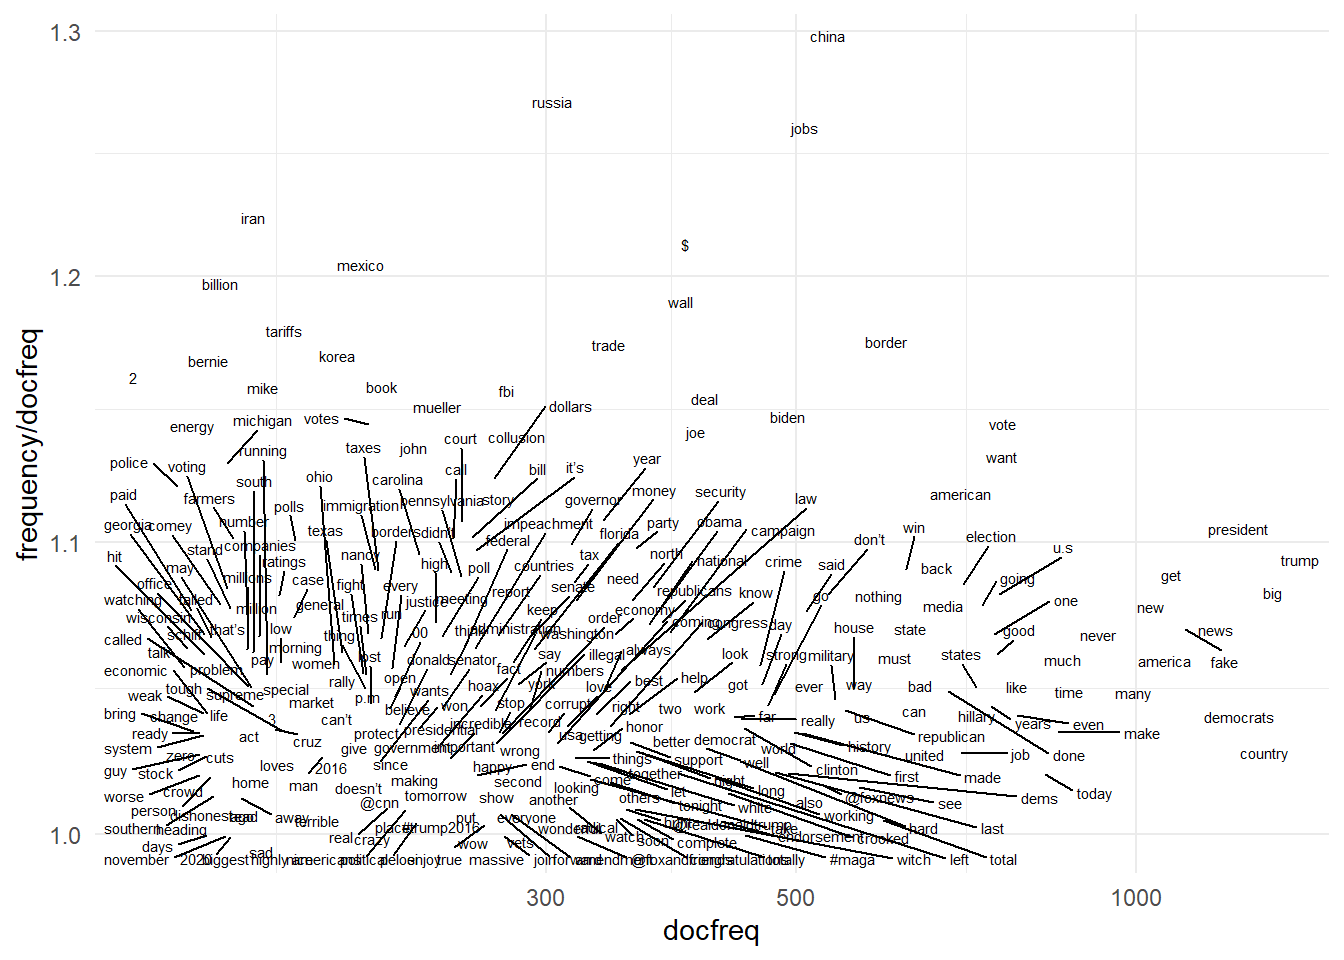
\includegraphics{q06_Analyse_quantitative_files/figure-pdf/613-1.pdf}

\section{Comptons les mots (toute cette partie est à déplacer au
chapitre
tokens)}\label{comptons-les-mots-toute-cette-partie-est-uxe0-duxe9placer-au-chapitre-tokens}

Il est temps de compter les mots, chacun d'entre eux, de se faire une
idée une idée de leurs fréquences, de leur distribution.

Souvent on éliminera ceux qui apparaissent de manière occasionnelle,
mais aussi ceux qui apparaissent systématiquement dans tous les textes.
Une fois ces deux filtrages effectués, le lexique est généralement de
l'ordre de 500 à 10000 mots.

Deux outils sont disponibles: les nuages de mots et les lollyplots. Les
premiers donnent une idée immédiates, les seconds se prêtent mieux à une
analyse systématique

\subsection{Les nuages de mots}\label{les-nuages-de-mots}

Ils sont devenus extrêmement populaires même si l'effet esthétique est
plus important que leur utilité analytique.

\href{https://cran.r-project.org/web/packages/ggwordcloud/vignettes/ggwordcloud.html}{\texttt{ggwordcloud}}

Pour l'application on prépare les données avec quanteda : on tokenise et
on construit le dfm (pour le détail voir chapitre tokenization), ce qui
nous permets notamment d'éliminer la ponctuation et les mots courants
(articles, déterminant etc) qui apportent peu de signification.

\begin{Shaded}
\begin{Highlighting}[]
\NormalTok{foo}\OtherTok{\textless{}{-}}\NormalTok{df }\SpecialCharTok{\%\textgreater{}\%} \FunctionTok{filter}\NormalTok{(isRetweet}\SpecialCharTok{==}\ConstantTok{FALSE}\NormalTok{) }\SpecialCharTok{\%\textgreater{}\%}
  \FunctionTok{filter}\NormalTok{( Year }\SpecialCharTok{\%in\%} \FunctionTok{c}\NormalTok{(}\StringTok{"2016"}\NormalTok{,}\StringTok{"2017"}\NormalTok{,}\StringTok{"2018"}\NormalTok{,}\StringTok{"2019"}\NormalTok{,}\StringTok{"2020"}\NormalTok{))}\CommentTok{\# on ne prend pas en compte les RT}

\NormalTok{toks}\OtherTok{\textless{}{-}} \FunctionTok{tokens}\NormalTok{(foo}\SpecialCharTok{$}\NormalTok{text) }\SpecialCharTok{\%\textgreater{}\%} 
  \FunctionTok{dfm}\NormalTok{(}\AttributeTok{remove\_punct =} \ConstantTok{TRUE}\NormalTok{,  }\AttributeTok{remove =} \FunctionTok{stopwords}\NormalTok{(}\StringTok{"english"}\NormalTok{))}

\FunctionTok{docvars}\NormalTok{(toks,}\StringTok{"Year"}\NormalTok{)}\OtherTok{\textless{}{-}}\NormalTok{foo}\SpecialCharTok{$}\NormalTok{Year}

\CommentTok{\#on se concentre du les termes utilisés 300 fois.  }

\NormalTok{foo}\OtherTok{\textless{}{-}}\NormalTok{toks }\SpecialCharTok{\%\textgreater{}\%} 
    \FunctionTok{dfm\_trim}\NormalTok{(}\AttributeTok{min\_termfreq =} \DecValTok{250}\NormalTok{, }\AttributeTok{verbose =} \ConstantTok{FALSE}\NormalTok{)}

\NormalTok{freq }\OtherTok{\textless{}{-}} \FunctionTok{textstat\_frequency}\NormalTok{(foo)}


\FunctionTok{ggplot}\NormalTok{(freq, }\FunctionTok{aes}\NormalTok{(}\AttributeTok{label =}\NormalTok{ feature)) }\SpecialCharTok{+}
  \FunctionTok{geom\_text\_wordcloud}\NormalTok{(}\FunctionTok{aes}\NormalTok{(}\AttributeTok{size=}\NormalTok{frequency, }\AttributeTok{color=}\NormalTok{rank)) }\SpecialCharTok{+}
  \FunctionTok{theme\_minimal}\NormalTok{() }\SpecialCharTok{+}  \FunctionTok{scale\_size\_area}\NormalTok{(}\AttributeTok{max\_size =} \DecValTok{10}\NormalTok{) }\SpecialCharTok{+} 
  \FunctionTok{scale\_color\_gradient}\NormalTok{(}\AttributeTok{low =}\NormalTok{ col\_1, }\AttributeTok{high =}\NormalTok{ col\_1b)}
\end{Highlighting}
\end{Shaded}

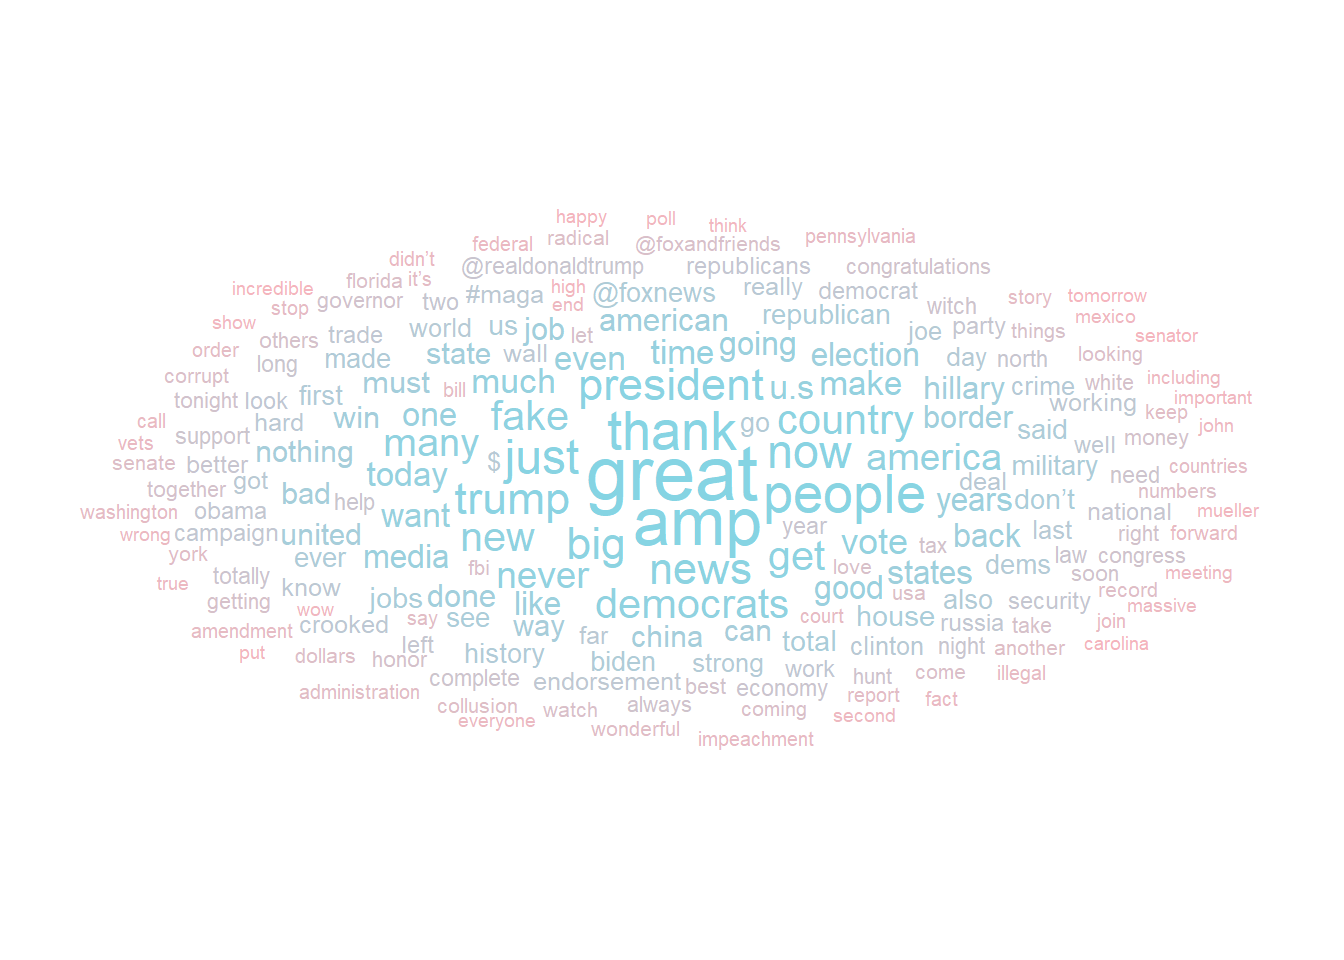
\includegraphics{q06_Analyse_quantitative_files/figure-pdf/614-1.pdf}

\begin{Shaded}
\begin{Highlighting}[]
\FunctionTok{ggsave}\NormalTok{(}\StringTok{"image/g0.jpg"}\NormalTok{, }\AttributeTok{plot=}\FunctionTok{last\_plot}\NormalTok{(), }\AttributeTok{width =} \DecValTok{27}\NormalTok{, }\AttributeTok{height =} \DecValTok{19}\NormalTok{, }\AttributeTok{units =} \StringTok{"cm"}\NormalTok{)}
\end{Highlighting}
\end{Shaded}

Et pour faire des comparaisons, entre l'année 2016 qui le conduit à être
élu, 2018 une année de midterm et 2020 année de sa défaite, on utilise
la même procédure mais on distingue un comptage de fréquence de mot par
période. Le ggplot est identique aux précédents mais comprend en plus
une géométrie ``facet\_wrap'' qui éclate le nuages de mot selon les 3
périodes étudiées.

\begin{Shaded}
\begin{Highlighting}[]
\NormalTok{foo}\OtherTok{\textless{}{-}}\NormalTok{toks }\SpecialCharTok{\%\textgreater{}\%} 
  \FunctionTok{dfm\_group}\NormalTok{(}\AttributeTok{groups =}\NormalTok{ Year) }\SpecialCharTok{\%\textgreater{}\%}
    \FunctionTok{dfm\_trim}\NormalTok{(}\AttributeTok{min\_termfreq =} \DecValTok{1}\NormalTok{, }\AttributeTok{verbose =} \ConstantTok{FALSE}\NormalTok{)}

\NormalTok{url\_regex }\OtherTok{\textless{}{-}} \StringTok{"http[s]?://(?:[a{-}zA{-}Z]|[0{-}9]|[${-}\_@.\&+]|[!*}\SpecialCharTok{\textbackslash{}\textbackslash{}}\StringTok{(}\SpecialCharTok{\textbackslash{}\textbackslash{}}\StringTok{),]|(?:\%[0{-}9a{-}fA{-}F][0{-}9a{-}fA{-}F]))+"}
  
\CommentTok{\#pour compter la fréquence des mots par année}
\NormalTok{freq }\OtherTok{\textless{}{-}} \FunctionTok{textstat\_frequency}\NormalTok{(foo, }\AttributeTok{group =}\NormalTok{Year) }\SpecialCharTok{\%\textgreater{}\%}
  \FunctionTok{mutate}\NormalTok{(}\AttributeTok{feature=}\FunctionTok{str\_remove\_all}\NormalTok{(feature, url\_regex))}\SpecialCharTok{|\textgreater{}}
  \FunctionTok{filter}\NormalTok{(}\SpecialCharTok{!}\FunctionTok{is.na}\NormalTok{(feature) }\SpecialCharTok{\&}\NormalTok{ frequency}\SpecialCharTok{\textgreater{}}\DecValTok{200}\NormalTok{ )}\SpecialCharTok{\%\textgreater{}\%}
  \FunctionTok{filter}\NormalTok{(feature}\SpecialCharTok{!=}\StringTok{"amp"}\NormalTok{)}
           

\FunctionTok{set.seed}\NormalTok{(}\DecValTok{42}\NormalTok{)}
\FunctionTok{library}\NormalTok{(ggwordcloud)}

\FunctionTok{ggplot}\NormalTok{(freq, }\FunctionTok{aes}\NormalTok{(}\AttributeTok{label =}\NormalTok{ feature)) }\SpecialCharTok{+}
  \FunctionTok{geom\_text\_wordcloud}\NormalTok{(}\FunctionTok{aes}\NormalTok{(}\AttributeTok{size=}\NormalTok{frequency, }\AttributeTok{color=}\NormalTok{rank)) }\SpecialCharTok{+}
  \FunctionTok{theme\_minimal}\NormalTok{()}\SpecialCharTok{+}
  \FunctionTok{facet\_wrap}\NormalTok{(}\FunctionTok{vars}\NormalTok{(group)) }\SpecialCharTok{+}  
  \FunctionTok{scale\_size\_area}\NormalTok{(}\AttributeTok{max\_size =} \DecValTok{8}\NormalTok{) }
\end{Highlighting}
\end{Shaded}

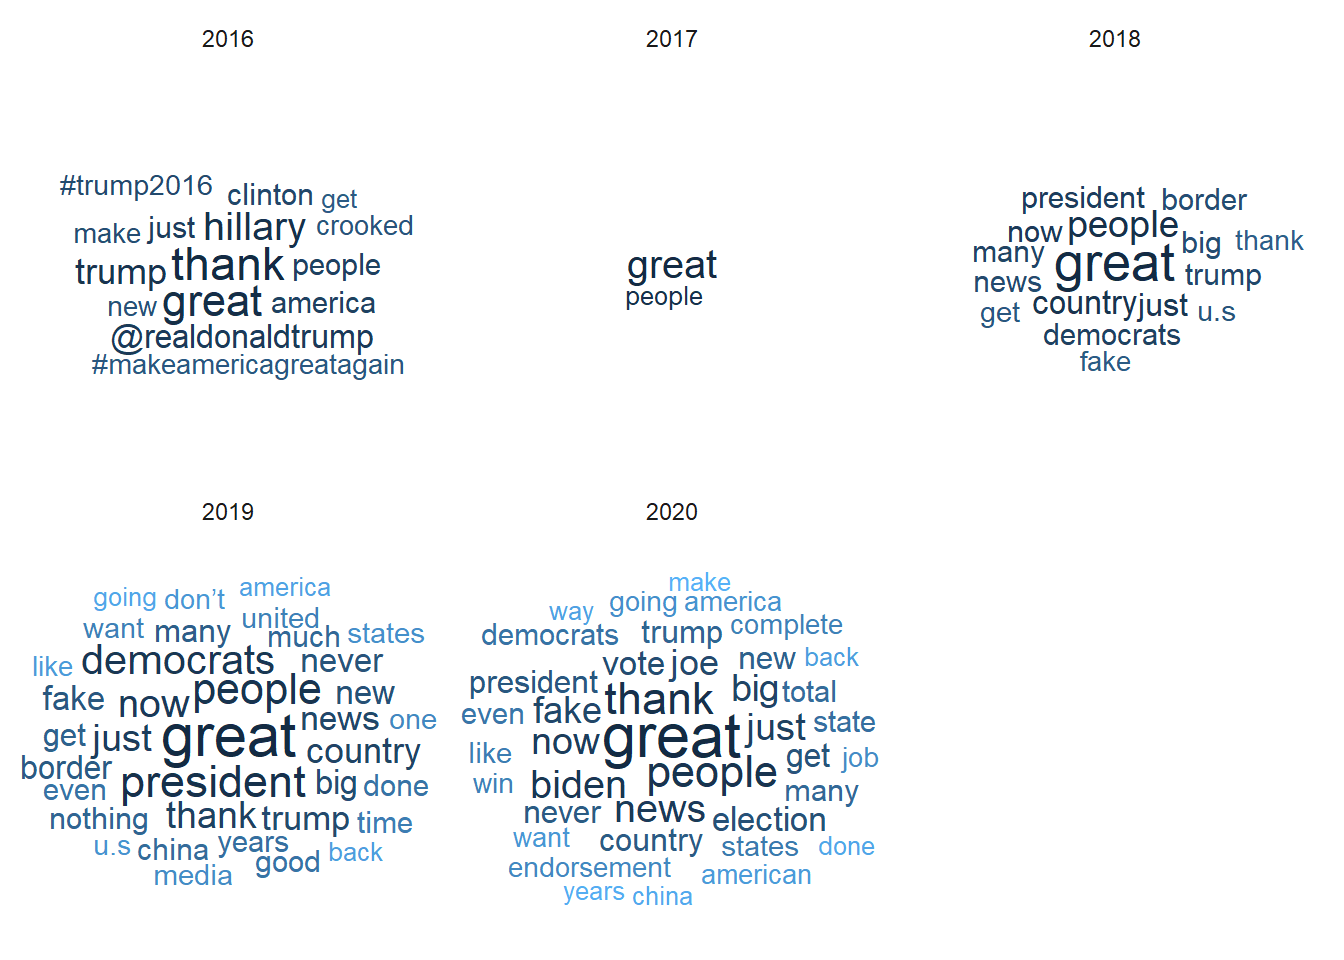
\includegraphics{q06_Analyse_quantitative_files/figure-pdf/615-1.pdf}

\begin{Shaded}
\begin{Highlighting}[]
\FunctionTok{ggsave}\NormalTok{(}\StringTok{"./image/g1.jpg"}\NormalTok{, }\AttributeTok{plot=}\FunctionTok{last\_plot}\NormalTok{(), }\AttributeTok{width =} \DecValTok{27}\NormalTok{, }\AttributeTok{height =} \DecValTok{19}\NormalTok{, }\AttributeTok{units =} \StringTok{"cm"}\NormalTok{)}
\end{Highlighting}
\end{Shaded}

\section{Conclusion}\label{conclusion-4}

Nous aurons appris à

\begin{itemize}
\tightlist
\item
  Compter le nombre de documents et leurs longueurs
\item
  Mesurer la complexité du langage
\item
  Mesurer la diversité de son vocabulaire.
\item
  A évaluer la concentration des sources
\item
  A se donner une première idée de la lexicographie
\end{itemize}

Ces mesures n'ont ne sens que si elles peuvent être l'objet de
comparaison :

\begin{itemize}
\tightlist
\item
  De manière interne la comparaison se fait dans dans le temps et à
  travers des segments. On s'intéresse moins aux niveaux, qu' à leurs
  différences.
\item
  De manière externe elle requiert un étalonnage. Comparer par rapport
  au français courant, à un niveau de langue soutenu, ou relâché.
  L'étalonnage revient à caractériser des types de corpus : presse,
  écriture savante, réseaux sociaux, publications officielles etc. On ne
  peut que souhaiter que des comparaisons systématiques soient engagées
  et compilées pour donner des points de repère quand on étudie un
  corpus particulier.
\end{itemize}

Elles participent à un premier niveau d'analyse du texte, en surface,
visant à apprécier la dynamique de sa production, à établir les échelles
d'analyse, à repérer les éléments structurels.

Le texte est une matière qui a un poids (le nombre de mot), une variété
(le nombre d'expressions), une complexité (les règles qui l'organisent).
nous venons de nous doter des premiers outils d'analyse, il est temps de
passer à la suite.

\bookmarksetup{startatroot}

\chapter{Jouer avec les jetons}\label{jouer-avec-les-jetons}

\begin{Shaded}
\begin{Highlighting}[]
\CommentTok{\#les librairies du chapître}
\FunctionTok{library}\NormalTok{(tidyverse)}
\FunctionTok{library}\NormalTok{(readr)}
\FunctionTok{library}\NormalTok{(tokenizers)}
\FunctionTok{library}\NormalTok{(quanteda)}
\FunctionTok{library}\NormalTok{(quanteda.textplots)}
\FunctionTok{library}\NormalTok{(flextable)}

\FunctionTok{theme\_set}\NormalTok{(}\FunctionTok{theme\_minimal}\NormalTok{()) }

\FunctionTok{set\_flextable\_defaults}\NormalTok{(}
  \AttributeTok{font.size =} \DecValTok{10}\NormalTok{, }\AttributeTok{theme\_fun =}\NormalTok{ theme\_vanilla,}
  \AttributeTok{padding =} \DecValTok{6}\NormalTok{,}
  \AttributeTok{background.color =} \StringTok{"\#EFEFEF"}\NormalTok{)}
\end{Highlighting}
\end{Shaded}

\textbf{Objectifs du chapitre :}

\emph{L'analyse du texte commence par découper les chaines de caractères
en unités pertinentes, c'est souvent le mot, ce peut être la syllabe, la
phrase, ou la lettre. Ces unités sont des jetons, les pièces élémentaire
d'un traitement plus sophistiqué. cette opération permet de quantifier
le texte et de le représenter sous la forme de dfm.}

L'étape initiale de toute analyse textuelle est de découper le texte en
unités d'analyse, les \emph{tokens}, ou jetons en français, ce qui
transforme le texte écrit pour la compréhension humaine en données
interprétables par l'ordinateur. Les \emph{tokens} utilisés peuvent
varier selon les objectifs de l'analyse et la nature du corpus, la
granularité peut être plus ou moins fine. Les \emph{tokens} peuvent
ainsi être :

\begin{itemize}
\tightlist
\item
  des lettres : c'est l'unité insécable.
\item
  des syllabes : ça permet de s'intéresser aux phonèmes.mais aussi
  d'extraire d'un mot les suffixes et préfixes, ainsi que les radicaux (
  la racine du mot, ex : dés-espéré-ment).
\item
  des mots : il s'agit du niveau le plus évident et le plus courant, que
  l'on privilégiera tout au long de ce livre, il présente aussi des
  difficultés car il ne coincide par avec l'unité de sens, par exemple
  avec les locutions: '' Président de la République'', ni avec les
  lexiques établis, ils peuvent prendre souvent la caractéristiques de
  \href{http://stella.atilf.fr/MotsFantomes/}{mots fantômes}
\item
  des phrases : c'est l'unité de langage, lui correspond un argument,
  une proposition ; l'usage du point suivi d'un espace et d'une
  majuscule est assez général pour les identifier.
\item
  des paragraphes : c'est une unité plus générale, qui souvent développe
  une idée.
\item
  des sections, des chapitres, ou des livres : selon la nature des
  documents, cela permet de découper le corpus en sous-unités.
\end{itemize}

Les \emph{tokenizers} sont les outils indispensables à cette tâche. Dans
cet ouvrage, nous nous concentrons sur l'étude des mots. Lors de cette
étude, un certain nombre de mots apparaissent de nombreuses fois, pour
permettre de donner du sens au langage humain, mais ils ne portent pas
en eux d'informations particulièrement pertinentes pour l'analyse : ce
sont les \emph{stopwords}, qu'il conviendra souvent d'éliminer.

Les n-grammes, quant à eux, représentent des suites de n \emph{tokens}.
Un unigramme est donc équivalent à un \emph{token}, un
digramme\footnote{En français digramme est la meilleure traduction de
  bigram, une bigramme en français est un mot dont les lettres peuvent
  former deux autres mot.} est une suite de deux \emph{tokens}, etc.
L'identification des n-grammes permet de détecter des suites de
\emph{tokens} qui reviennent plus souvent que leur probabilité
d'occurrences. Si l'on se concentre sur les mots, nous sommes alors face
à une unité sémantique, comme on le comprend facilement avec le digramme
`Assemblée Nationale' dont le sens est plus que ses constituants.

Tokeniser revient donc à découper le texte pour en construire une
représentation quantitative.C'est d'ailleurs une des spécificités des
grands modèles de langage qui s'intréesse moins aux mots, qu'à ses
décompositions, telles qu'un nombre limité( \textasciitilde30 000)
permette de générer la plupart des graphies et au passage de supporter
les dysgraphies.

\section{Quelques exercices de
tokenization}\label{quelques-exercices-de-tokenization}

\subsection{Les lettres}\label{les-lettres}

Commençons par un exemple simple, à l'aide d'une courte citation de Max
Weber. On choisit les lettres pour unité de découpe, et l'on utilise le
package
\href{https://cran.r-project.org/web/packages/tokenizers/vignettes/introduction-to-tokenizers.html}{`tokenizer'}.
Automatiquement, `tokenizer' met le texte en minuscule et élimine la
ponctuation

\begin{Shaded}
\begin{Highlighting}[]
\CommentTok{\#Les données}
\NormalTok{MaxWeber }\OtherTok{\textless{}{-}} \FunctionTok{paste0}\NormalTok{(}\StringTok{"Bureaucratie: le moyen le plus rationnel que l’on connaisse pour exercer un contrôle impératif sur des êtres humains."}\NormalTok{)}

\CommentTok{\#On tokenise, plus on transforme en dataframe le résultat.}
\NormalTok{toc\_maxweber}\OtherTok{\textless{}{-}}\FunctionTok{tokenize\_characters}\NormalTok{(MaxWeber)}\SpecialCharTok{\%\textgreater{}\%}
        \FunctionTok{as.data.frame}\NormalTok{()}\SpecialCharTok{\%\textgreater{}\%}
        \FunctionTok{rename}\NormalTok{(}\AttributeTok{tokens=}\DecValTok{1}\NormalTok{)}

\CommentTok{\#On compte pour chaque token sa fréquence d\textquotesingle{}apparition}
\NormalTok{foo}\OtherTok{\textless{}{-}}\NormalTok{toc\_maxweber }\SpecialCharTok{\%\textgreater{}\%} 
        \FunctionTok{group\_by}\NormalTok{(tokens)}\SpecialCharTok{\%\textgreater{}\%} 
        \FunctionTok{summarise}\NormalTok{(}\AttributeTok{n=}\FunctionTok{n}\NormalTok{())}\SpecialCharTok{\%\textgreater{}\%}
        \FunctionTok{filter}\NormalTok{(n}\SpecialCharTok{\textgreater{}}\DecValTok{0}\NormalTok{)}

\CommentTok{\#On représente par un diagramme en barre cette distribution des occuences d\textquotesingle{}apparition, en classant les tokens par fréquence}
\FunctionTok{ggplot}\NormalTok{(foo, }\FunctionTok{aes}\NormalTok{(}\AttributeTok{x=}\FunctionTok{reorder}\NormalTok{(tokens,n), }\AttributeTok{y=}\NormalTok{n))}\SpecialCharTok{+}
               \FunctionTok{geom\_bar}\NormalTok{(}\AttributeTok{stat=}\StringTok{"identity"}\NormalTok{, }\AttributeTok{fill=}\StringTok{"royalblue"}\NormalTok{)}\SpecialCharTok{+}
        \FunctionTok{annotate}\NormalTok{(}\StringTok{"text"}\NormalTok{, }\AttributeTok{x=}\DecValTok{10}\NormalTok{,}\AttributeTok{y=}\DecValTok{10}\NormalTok{, }\AttributeTok{label=}\FunctionTok{paste}\NormalTok{(}\StringTok{"nombre de tokens ="}\NormalTok{, }\FunctionTok{nrow}\NormalTok{(toc\_maxweber)))}\SpecialCharTok{+}
               \FunctionTok{coord\_flip}\NormalTok{()}\SpecialCharTok{+}
        \FunctionTok{labs}\NormalTok{(}\AttributeTok{title =} \StringTok{"Fréquence des tokens, unité = lettres"}\NormalTok{, }
             \AttributeTok{x=}\StringTok{"tokens"}\NormalTok{, }
             \AttributeTok{y=}\StringTok{"nombre d\textquotesingle{}occurences"}\NormalTok{, }
             \AttributeTok{caption =}\StringTok{" \textquotesingle{}Bureaucratie: le moyen le plus rationnel que l’on connaisse pour exercer un contrôle impératif sur des êtres humains.\textquotesingle{} "}\NormalTok{)}
\end{Highlighting}
\end{Shaded}

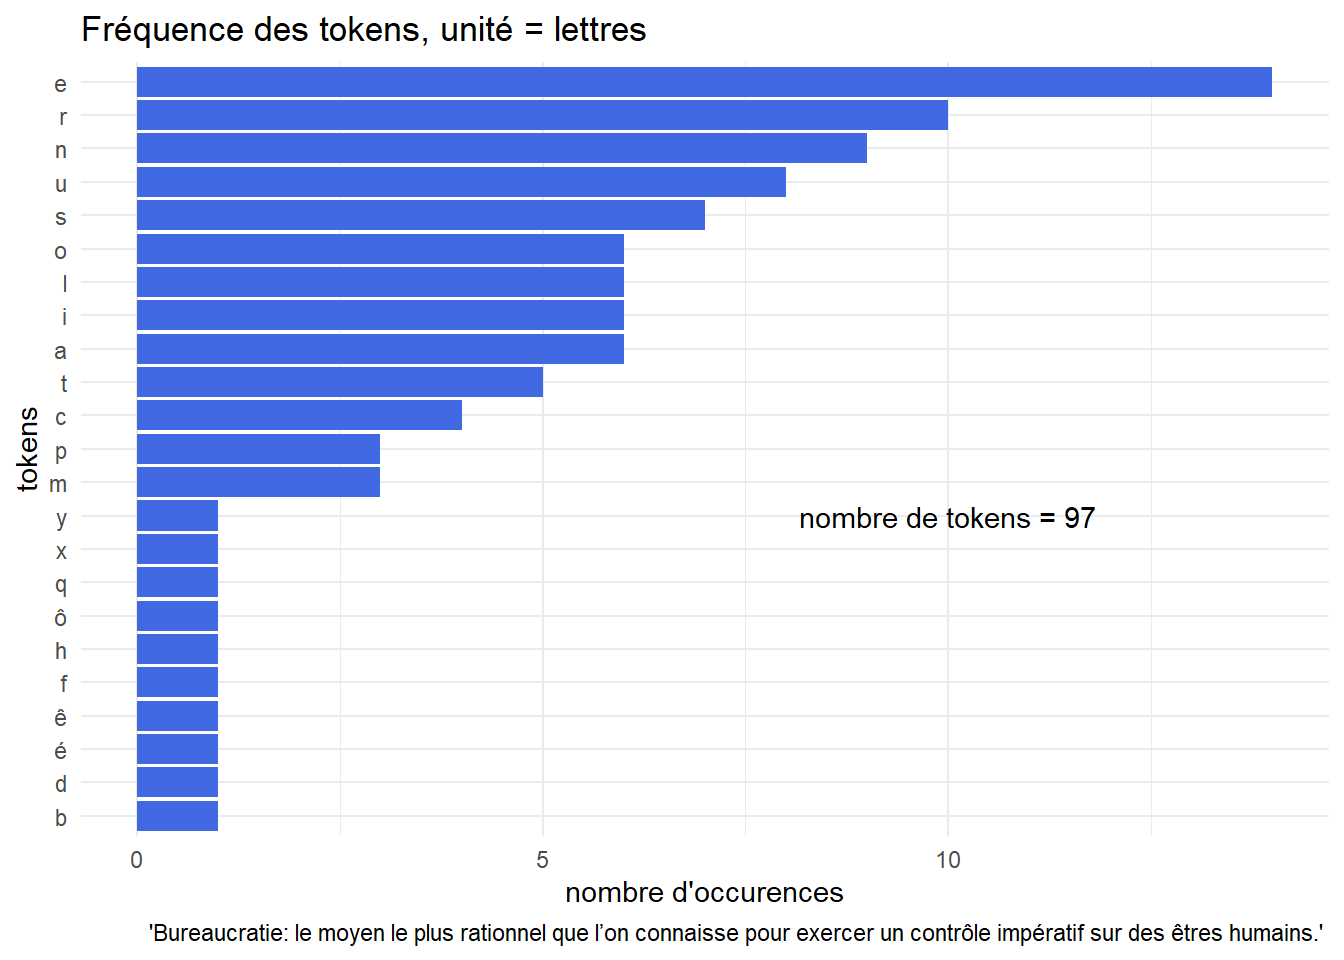
\includegraphics{q07_tokenisation_files/figure-pdf/601-1.pdf}

\subsection{les mots}\label{les-mots}

\begin{Shaded}
\begin{Highlighting}[]
\CommentTok{\#Les données}

\NormalTok{MaxWeber }\OtherTok{\textless{}{-}} \FunctionTok{paste0}\NormalTok{(}\StringTok{"Bureaucratie: le moyen le plus rationnel que l’on connaisse pour exercer un contrôle impératif sur des êtres humains. La bureaucratie est une forme d\textquotesingle{}organisation générale caractérisée par la prépondérance des règles et de procédures qui sont appliquées de façon impersonnelle par des agents spécialisés. Ces agents appliquent les règles sans discuter des objectifs ou des raisons qui les fondent. Ils doivent faire preuve de neutralité et oublier leurs propres intérêts personnels au profit de l’intérêt général."}\NormalTok{)}

\CommentTok{\#On tokenise, plus on transforme en dataframe le résultat. le strp\_punc écarte la ponctuation du processus.}
\NormalTok{toc\_maxweber}\OtherTok{\textless{}{-}}\FunctionTok{tokenize\_words}\NormalTok{(MaxWeber,}\AttributeTok{strip\_punct=}\ConstantTok{TRUE}\NormalTok{)}\SpecialCharTok{\%\textgreater{}\%}
        \FunctionTok{as.data.frame}\NormalTok{()}\SpecialCharTok{\%\textgreater{}\%}
        \FunctionTok{rename}\NormalTok{(}\AttributeTok{tokens=}\DecValTok{1}\NormalTok{)}

\CommentTok{\#On compte pour chaque token sa fréquence d\textquotesingle{}apparition}
\NormalTok{foo}\OtherTok{\textless{}{-}}\NormalTok{toc\_maxweber }\SpecialCharTok{\%\textgreater{}\%}\FunctionTok{mutate}\NormalTok{(}\AttributeTok{n=}\DecValTok{1}\NormalTok{) }\SpecialCharTok{\%\textgreater{}\%} 
        \FunctionTok{group\_by}\NormalTok{(tokens)}\SpecialCharTok{\%\textgreater{}\%} 
        \FunctionTok{summarise}\NormalTok{(}\AttributeTok{n=}\FunctionTok{sum}\NormalTok{(n))}

\CommentTok{\#On représente par un diagramme en barre cette distribution des occurrences, en classant les tokens par fréquence}
\FunctionTok{ggplot}\NormalTok{(foo, }\FunctionTok{aes}\NormalTok{(}\AttributeTok{x=}\FunctionTok{reorder}\NormalTok{(tokens,n), }\AttributeTok{y=}\NormalTok{n))}\SpecialCharTok{+}
               \FunctionTok{geom\_bar}\NormalTok{(}\AttributeTok{stat=}\StringTok{"identity"}\NormalTok{, }\AttributeTok{fill=}\StringTok{"royalblue"}\NormalTok{)}\SpecialCharTok{+}
        \FunctionTok{annotate}\NormalTok{(}\StringTok{"text"}\NormalTok{, }\AttributeTok{x=}\DecValTok{10}\NormalTok{,}\AttributeTok{y=}\DecValTok{4}\NormalTok{, }\AttributeTok{label=}\FunctionTok{paste}\NormalTok{(}\StringTok{"nombre de tokens ="}\NormalTok{, }\FunctionTok{nrow}\NormalTok{(toc\_maxweber)))}\SpecialCharTok{+}
               \FunctionTok{coord\_flip}\NormalTok{()}\SpecialCharTok{+}\FunctionTok{labs}\NormalTok{(}\AttributeTok{title =} \StringTok{"Fréquence des tokens, unité = mots"}\NormalTok{, }\AttributeTok{x=}\StringTok{"tokens"}\NormalTok{, }\AttributeTok{y=}\StringTok{"nombre d\textquotesingle{}occurences"}\NormalTok{, }\AttributeTok{caption =}\StringTok{" \textquotesingle{}Bureaucratie: le moyen le plus rationnel que l’on connaisse pour exercer un contrôle impératif sur des êtres humains.\textquotesingle{} "}\NormalTok{)}
\end{Highlighting}
\end{Shaded}

\includegraphics{q07_tokenisation_files/figure-pdf/602-1.pdf}

On peut également constater que certains mots sont proches, par exemple
les deux derniers sur le graphiques précédents qui sont des déclinaisons
du verbe appliquer. Il peut alors être pertinent de regrouper ces
différentes formes verbales (comme un mot au singulier et au pluriel, au
féminin et au masculin, ou conjugué sous différentes formes), pour
faciliter l'analyse. C'est ce qu'on fait avec les opérations de
\emph{stemming} ou de lemmatisation, présentées au chapitre 8.

\subsection{Les phrases}\label{les-phrases}

On reproduit les mêmes opérations, mais cette fois sur les phrases de
l'exemple précédent.

\begin{Shaded}
\begin{Highlighting}[]
\FunctionTok{tokenize\_sentences}\NormalTok{(MaxWeber)}\SpecialCharTok{\%\textgreater{}\%}
  \FunctionTok{as.data.frame}\NormalTok{()}\SpecialCharTok{\%\textgreater{}\%}
  \FunctionTok{rename}\NormalTok{(}\AttributeTok{tokens=}\DecValTok{1}\NormalTok{)}\SpecialCharTok{\%\textgreater{}\%}
  \FunctionTok{flextable}\NormalTok{(}\AttributeTok{cwidth =} \DecValTok{6}\NormalTok{)}
\end{Highlighting}
\end{Shaded}

\global\setlength{\Oldarrayrulewidth}{\arrayrulewidth}

\global\setlength{\Oldtabcolsep}{\tabcolsep}

\setlength{\tabcolsep}{0pt}

\renewcommand*{\arraystretch}{1.5}



\providecommand{\ascline}[3]{\noalign{\global\arrayrulewidth #1}\arrayrulecolor[HTML]{#2}\cline{#3}}

\begin{longtable*}[c]{|p{6.00in}}



\hhline{>{\arrayrulecolor[HTML]{666666}\global\arrayrulewidth=1.5pt}-}

\multicolumn{1}{>{\cellcolor[HTML]{EFEFEF}\raggedright}m{\dimexpr 6in+0\tabcolsep}}{\textcolor[HTML]{000000}{\fontsize{10}{10}\selectfont{\textbf{tokens}}}} \\

\noalign{\global\arrayrulewidth 0pt}\arrayrulecolor[HTML]{000000}

\hhline{>{\arrayrulecolor[HTML]{666666}\global\arrayrulewidth=1.5pt}-}\endfirsthead 

\hhline{>{\arrayrulecolor[HTML]{666666}\global\arrayrulewidth=1.5pt}-}

\multicolumn{1}{>{\cellcolor[HTML]{EFEFEF}\raggedright}m{\dimexpr 6in+0\tabcolsep}}{\textcolor[HTML]{000000}{\fontsize{10}{10}\selectfont{\textbf{tokens}}}} \\

\noalign{\global\arrayrulewidth 0pt}\arrayrulecolor[HTML]{000000}

\hhline{>{\arrayrulecolor[HTML]{666666}\global\arrayrulewidth=1.5pt}-}\endhead



\multicolumn{1}{>{\cellcolor[HTML]{EFEFEF}\raggedright}m{\dimexpr 6in+0\tabcolsep}}{\textcolor[HTML]{000000}{\fontsize{10}{10}\selectfont{Bureaucratie:\ le\ moyen\ le\ plus\ rationnel\ que\ l’on\ connaisse\ pour\ exercer\ un\ contrôle\ impératif\ sur\ des\ êtres\ humains.}}} \\

\noalign{\global\arrayrulewidth 0pt}\arrayrulecolor[HTML]{000000}

\hhline{>{\arrayrulecolor[HTML]{666666}\global\arrayrulewidth=0.75pt}-}



\multicolumn{1}{>{\cellcolor[HTML]{EFEFEF}\raggedright}m{\dimexpr 6in+0\tabcolsep}}{\textcolor[HTML]{000000}{\fontsize{10}{10}\selectfont{La\ bureaucratie\ est\ une\ forme\ d'organisation\ générale\ caractérisée\ par\ la\ prépondérance\ des\ règles\ et\ de\ procédures\ qui\ sont\ appliquées\ de\ façon\ impersonnelle\ par\ des\ agents\ spécialisés.}}} \\

\noalign{\global\arrayrulewidth 0pt}\arrayrulecolor[HTML]{000000}

\hhline{>{\arrayrulecolor[HTML]{666666}\global\arrayrulewidth=0.75pt}-}



\multicolumn{1}{>{\cellcolor[HTML]{EFEFEF}\raggedright}m{\dimexpr 6in+0\tabcolsep}}{\textcolor[HTML]{000000}{\fontsize{10}{10}\selectfont{Ces\ agents\ appliquent\ les\ règles\ sans\ discuter\ des\ objectifs\ ou\ des\ raisons\ qui\ les\ fondent.}}} \\

\noalign{\global\arrayrulewidth 0pt}\arrayrulecolor[HTML]{000000}

\hhline{>{\arrayrulecolor[HTML]{666666}\global\arrayrulewidth=0.75pt}-}



\multicolumn{1}{>{\cellcolor[HTML]{EFEFEF}\raggedright}m{\dimexpr 6in+0\tabcolsep}}{\textcolor[HTML]{000000}{\fontsize{10}{10}\selectfont{Ils\ doivent\ faire\ preuve\ de\ neutralité\ et\ oublier\ leurs\ propres\ intérêts\ personnels\ au\ profit\ de\ l’intérêt\ général.}}} \\

\noalign{\global\arrayrulewidth 0pt}\arrayrulecolor[HTML]{000000}

\hhline{>{\arrayrulecolor[HTML]{666666}\global\arrayrulewidth=1.5pt}-}



\end{longtable*}



\arrayrulecolor[HTML]{000000}

\global\setlength{\arrayrulewidth}{\Oldarrayrulewidth}

\global\setlength{\tabcolsep}{\Oldtabcolsep}

\renewcommand*{\arraystretch}{1}

\section{N-grammes}\label{n-grammes}

Les n-grammes sont des séquences de n \emph{tokens}, généralement
consécutifs. Sur la d'un base d'un corpus important on peut calculer la
probabilité d'apparition d'un n-gramme. C'est l'exercice auquel une
équipe de google s'est attelé avec le
\href{https://books.google.com/ngrams/}{Books Ngram Viewer}. et dont
nous encourageons l'étude détaillée.

L'article original doit aussi être lu. Sur la base de 5 millions de
livres numérisés en 2011 et représentant 4\% du nombre total de livres à
jamais publiés à ce moment, être lu aussi, il montre que, pour
l'anglais, chaque année 8500 mots entrent dans le lexique, sans que les
dictionnaires, pour des raisons évidentes de concision, n'en font
l'inventaire. Le webster comprend 300 000 mots, alors que pour l'anglais
l'estimation du nombre de termes différents, est passé de l'ordre de 500
000 en 1900, à plus d'1.5 million en 2000. Il donne aussi une dimension
au lexique : celle de sa densité. Dans un corpus, à un moment donné
quelle est la probabilité d'observer un token donné (au plus simple un
mot). Sur un corpus de 500 milliards de termes (pour toutes les langues
traitées), un mot qui apparaît une fois sur 1000 ( 10\^{}-3), apparaît 5
millions de fois, s'il apparaît une fois sur 1 million, il apparaît 5000
fois. L'échelle de mesure est ainsi la fréquence : 10-3, 10-5, 10-6
\ldots.

La notion de ngram au-delà de son apparence de tautologie possède aussi
un intérêt théorique majeure. Les ngram sont des chaines de markov.
Intérêt théorique des n gram : ce sont des chaines de markov.

\href{https://fr.wikipedia.org/wiki/N-gramme}{Processus de markov}

Pour comprendre l'importance de ce concept on peut considérer au moins 3
applications remarquables

Application à l'auto-complétion . Son efficacité dépend naturellement de
la taille des données récoltées. On comprend que pour google il est aisé
d'être précis dans l'estimation de ces probabilités!

Mais mieux encore, ces propriété markovienne ( probabilistique)
permettent aussi la correction d'erreur avec l'algorithme de Viterbi
https://fr.wikipedia.org/wiki/Algorithme\_de\_Viterbi

\begin{itemize}
\tightlist
\item
  Le principe de `textcat' est fondée sur ces n-grammes de lettre.
  Chaque langue se caractérise par une distribution particulière des
  n-grammes. Pour décider de l'appartenance d'un texte à une langue, si
  on dispose des profils de distribution, on compare la distribution des
  n-grammes du texte à ces références. On peut ainsi calculer une
  distance et attribuer le texte à la langue dont il est le plus proche.
\end{itemize}

\subsection{Mise en oeuvre}\label{mise-en-oeuvre}

Si la notion est simple, sa mise en oeuvre l'est presque autant. Nous
l'illustrons avec une séries d'exemples et le package ``tokenizer'' qui
a ici un avantage pédagogique. On étudiera plus loin les ressources de
``quanteda''.

On commence de suite par un exemple sur les lettres. c'est de pure
forme. On sélectionne les ngrammes (k\textgreater1 et k\textgreater4)
dont la fréquence est supérieure à trois.

\begin{Shaded}
\begin{Highlighting}[]
\CommentTok{\#tokenization des lettres}
\NormalTok{toc\_maxweber}\OtherTok{\textless{}{-}}\FunctionTok{tokenize\_character\_shingles}\NormalTok{(MaxWeber,}\AttributeTok{n=}\DecValTok{3}\NormalTok{, }\AttributeTok{n\_min=}\DecValTok{2}\NormalTok{) }\SpecialCharTok{\%\textgreater{}\%}
        \FunctionTok{as.data.frame}\NormalTok{()}\SpecialCharTok{\%\textgreater{}\%}
  \FunctionTok{rename}\NormalTok{(}\AttributeTok{tokens=}\DecValTok{1}\NormalTok{)}

\FunctionTok{flextable}\NormalTok{(}\FunctionTok{head}\NormalTok{(toc\_maxweber, }\AttributeTok{n=}\DecValTok{20}\NormalTok{))}
\end{Highlighting}
\end{Shaded}

\global\setlength{\Oldarrayrulewidth}{\arrayrulewidth}

\global\setlength{\Oldtabcolsep}{\tabcolsep}

\setlength{\tabcolsep}{0pt}

\renewcommand*{\arraystretch}{1.5}



\providecommand{\ascline}[3]{\noalign{\global\arrayrulewidth #1}\arrayrulecolor[HTML]{#2}\cline{#3}}

\begin{longtable*}[c]{|p{0.75in}}



\hhline{>{\arrayrulecolor[HTML]{666666}\global\arrayrulewidth=1.5pt}-}

\multicolumn{1}{>{\cellcolor[HTML]{EFEFEF}\raggedright}m{\dimexpr 0.75in+0\tabcolsep}}{\textcolor[HTML]{000000}{\fontsize{10}{10}\selectfont{\textbf{tokens}}}} \\

\noalign{\global\arrayrulewidth 0pt}\arrayrulecolor[HTML]{000000}

\hhline{>{\arrayrulecolor[HTML]{666666}\global\arrayrulewidth=1.5pt}-}\endfirsthead 

\hhline{>{\arrayrulecolor[HTML]{666666}\global\arrayrulewidth=1.5pt}-}

\multicolumn{1}{>{\cellcolor[HTML]{EFEFEF}\raggedright}m{\dimexpr 0.75in+0\tabcolsep}}{\textcolor[HTML]{000000}{\fontsize{10}{10}\selectfont{\textbf{tokens}}}} \\

\noalign{\global\arrayrulewidth 0pt}\arrayrulecolor[HTML]{000000}

\hhline{>{\arrayrulecolor[HTML]{666666}\global\arrayrulewidth=1.5pt}-}\endhead



\multicolumn{1}{>{\cellcolor[HTML]{EFEFEF}\raggedright}m{\dimexpr 0.75in+0\tabcolsep}}{\textcolor[HTML]{000000}{\fontsize{10}{10}\selectfont{bu}}} \\

\noalign{\global\arrayrulewidth 0pt}\arrayrulecolor[HTML]{000000}

\hhline{>{\arrayrulecolor[HTML]{666666}\global\arrayrulewidth=0.75pt}-}



\multicolumn{1}{>{\cellcolor[HTML]{EFEFEF}\raggedright}m{\dimexpr 0.75in+0\tabcolsep}}{\textcolor[HTML]{000000}{\fontsize{10}{10}\selectfont{bur}}} \\

\noalign{\global\arrayrulewidth 0pt}\arrayrulecolor[HTML]{000000}

\hhline{>{\arrayrulecolor[HTML]{666666}\global\arrayrulewidth=0.75pt}-}



\multicolumn{1}{>{\cellcolor[HTML]{EFEFEF}\raggedright}m{\dimexpr 0.75in+0\tabcolsep}}{\textcolor[HTML]{000000}{\fontsize{10}{10}\selectfont{ur}}} \\

\noalign{\global\arrayrulewidth 0pt}\arrayrulecolor[HTML]{000000}

\hhline{>{\arrayrulecolor[HTML]{666666}\global\arrayrulewidth=0.75pt}-}



\multicolumn{1}{>{\cellcolor[HTML]{EFEFEF}\raggedright}m{\dimexpr 0.75in+0\tabcolsep}}{\textcolor[HTML]{000000}{\fontsize{10}{10}\selectfont{ure}}} \\

\noalign{\global\arrayrulewidth 0pt}\arrayrulecolor[HTML]{000000}

\hhline{>{\arrayrulecolor[HTML]{666666}\global\arrayrulewidth=0.75pt}-}



\multicolumn{1}{>{\cellcolor[HTML]{EFEFEF}\raggedright}m{\dimexpr 0.75in+0\tabcolsep}}{\textcolor[HTML]{000000}{\fontsize{10}{10}\selectfont{re}}} \\

\noalign{\global\arrayrulewidth 0pt}\arrayrulecolor[HTML]{000000}

\hhline{>{\arrayrulecolor[HTML]{666666}\global\arrayrulewidth=0.75pt}-}



\multicolumn{1}{>{\cellcolor[HTML]{EFEFEF}\raggedright}m{\dimexpr 0.75in+0\tabcolsep}}{\textcolor[HTML]{000000}{\fontsize{10}{10}\selectfont{rea}}} \\

\noalign{\global\arrayrulewidth 0pt}\arrayrulecolor[HTML]{000000}

\hhline{>{\arrayrulecolor[HTML]{666666}\global\arrayrulewidth=0.75pt}-}



\multicolumn{1}{>{\cellcolor[HTML]{EFEFEF}\raggedright}m{\dimexpr 0.75in+0\tabcolsep}}{\textcolor[HTML]{000000}{\fontsize{10}{10}\selectfont{ea}}} \\

\noalign{\global\arrayrulewidth 0pt}\arrayrulecolor[HTML]{000000}

\hhline{>{\arrayrulecolor[HTML]{666666}\global\arrayrulewidth=0.75pt}-}



\multicolumn{1}{>{\cellcolor[HTML]{EFEFEF}\raggedright}m{\dimexpr 0.75in+0\tabcolsep}}{\textcolor[HTML]{000000}{\fontsize{10}{10}\selectfont{eau}}} \\

\noalign{\global\arrayrulewidth 0pt}\arrayrulecolor[HTML]{000000}

\hhline{>{\arrayrulecolor[HTML]{666666}\global\arrayrulewidth=0.75pt}-}



\multicolumn{1}{>{\cellcolor[HTML]{EFEFEF}\raggedright}m{\dimexpr 0.75in+0\tabcolsep}}{\textcolor[HTML]{000000}{\fontsize{10}{10}\selectfont{au}}} \\

\noalign{\global\arrayrulewidth 0pt}\arrayrulecolor[HTML]{000000}

\hhline{>{\arrayrulecolor[HTML]{666666}\global\arrayrulewidth=0.75pt}-}



\multicolumn{1}{>{\cellcolor[HTML]{EFEFEF}\raggedright}m{\dimexpr 0.75in+0\tabcolsep}}{\textcolor[HTML]{000000}{\fontsize{10}{10}\selectfont{auc}}} \\

\noalign{\global\arrayrulewidth 0pt}\arrayrulecolor[HTML]{000000}

\hhline{>{\arrayrulecolor[HTML]{666666}\global\arrayrulewidth=0.75pt}-}



\multicolumn{1}{>{\cellcolor[HTML]{EFEFEF}\raggedright}m{\dimexpr 0.75in+0\tabcolsep}}{\textcolor[HTML]{000000}{\fontsize{10}{10}\selectfont{uc}}} \\

\noalign{\global\arrayrulewidth 0pt}\arrayrulecolor[HTML]{000000}

\hhline{>{\arrayrulecolor[HTML]{666666}\global\arrayrulewidth=0.75pt}-}



\multicolumn{1}{>{\cellcolor[HTML]{EFEFEF}\raggedright}m{\dimexpr 0.75in+0\tabcolsep}}{\textcolor[HTML]{000000}{\fontsize{10}{10}\selectfont{ucr}}} \\

\noalign{\global\arrayrulewidth 0pt}\arrayrulecolor[HTML]{000000}

\hhline{>{\arrayrulecolor[HTML]{666666}\global\arrayrulewidth=0.75pt}-}



\multicolumn{1}{>{\cellcolor[HTML]{EFEFEF}\raggedright}m{\dimexpr 0.75in+0\tabcolsep}}{\textcolor[HTML]{000000}{\fontsize{10}{10}\selectfont{cr}}} \\

\noalign{\global\arrayrulewidth 0pt}\arrayrulecolor[HTML]{000000}

\hhline{>{\arrayrulecolor[HTML]{666666}\global\arrayrulewidth=0.75pt}-}



\multicolumn{1}{>{\cellcolor[HTML]{EFEFEF}\raggedright}m{\dimexpr 0.75in+0\tabcolsep}}{\textcolor[HTML]{000000}{\fontsize{10}{10}\selectfont{cra}}} \\

\noalign{\global\arrayrulewidth 0pt}\arrayrulecolor[HTML]{000000}

\hhline{>{\arrayrulecolor[HTML]{666666}\global\arrayrulewidth=0.75pt}-}



\multicolumn{1}{>{\cellcolor[HTML]{EFEFEF}\raggedright}m{\dimexpr 0.75in+0\tabcolsep}}{\textcolor[HTML]{000000}{\fontsize{10}{10}\selectfont{ra}}} \\

\noalign{\global\arrayrulewidth 0pt}\arrayrulecolor[HTML]{000000}

\hhline{>{\arrayrulecolor[HTML]{666666}\global\arrayrulewidth=0.75pt}-}



\multicolumn{1}{>{\cellcolor[HTML]{EFEFEF}\raggedright}m{\dimexpr 0.75in+0\tabcolsep}}{\textcolor[HTML]{000000}{\fontsize{10}{10}\selectfont{rat}}} \\

\noalign{\global\arrayrulewidth 0pt}\arrayrulecolor[HTML]{000000}

\hhline{>{\arrayrulecolor[HTML]{666666}\global\arrayrulewidth=0.75pt}-}



\multicolumn{1}{>{\cellcolor[HTML]{EFEFEF}\raggedright}m{\dimexpr 0.75in+0\tabcolsep}}{\textcolor[HTML]{000000}{\fontsize{10}{10}\selectfont{at}}} \\

\noalign{\global\arrayrulewidth 0pt}\arrayrulecolor[HTML]{000000}

\hhline{>{\arrayrulecolor[HTML]{666666}\global\arrayrulewidth=0.75pt}-}



\multicolumn{1}{>{\cellcolor[HTML]{EFEFEF}\raggedright}m{\dimexpr 0.75in+0\tabcolsep}}{\textcolor[HTML]{000000}{\fontsize{10}{10}\selectfont{ati}}} \\

\noalign{\global\arrayrulewidth 0pt}\arrayrulecolor[HTML]{000000}

\hhline{>{\arrayrulecolor[HTML]{666666}\global\arrayrulewidth=0.75pt}-}



\multicolumn{1}{>{\cellcolor[HTML]{EFEFEF}\raggedright}m{\dimexpr 0.75in+0\tabcolsep}}{\textcolor[HTML]{000000}{\fontsize{10}{10}\selectfont{ti}}} \\

\noalign{\global\arrayrulewidth 0pt}\arrayrulecolor[HTML]{000000}

\hhline{>{\arrayrulecolor[HTML]{666666}\global\arrayrulewidth=0.75pt}-}



\multicolumn{1}{>{\cellcolor[HTML]{EFEFEF}\raggedright}m{\dimexpr 0.75in+0\tabcolsep}}{\textcolor[HTML]{000000}{\fontsize{10}{10}\selectfont{tie}}} \\

\noalign{\global\arrayrulewidth 0pt}\arrayrulecolor[HTML]{000000}

\hhline{>{\arrayrulecolor[HTML]{666666}\global\arrayrulewidth=1.5pt}-}



\end{longtable*}



\arrayrulecolor[HTML]{000000}

\global\setlength{\arrayrulewidth}{\Oldarrayrulewidth}

\global\setlength{\tabcolsep}{\Oldtabcolsep}

\renewcommand*{\arraystretch}{1}

\begin{Shaded}
\begin{Highlighting}[]
\NormalTok{foo}\OtherTok{\textless{}{-}}\NormalTok{toc\_maxweber }\SpecialCharTok{\%\textgreater{}\%}\FunctionTok{mutate}\NormalTok{(}\AttributeTok{n=}\DecValTok{1}\NormalTok{) }\SpecialCharTok{\%\textgreater{}\%} 
        \FunctionTok{group\_by}\NormalTok{(tokens)}\SpecialCharTok{\%\textgreater{}\%} 
        \FunctionTok{summarise}\NormalTok{(}\AttributeTok{n=}\FunctionTok{sum}\NormalTok{(n))}\SpecialCharTok{\%\textgreater{}\%}
  \FunctionTok{filter}\NormalTok{(n}\SpecialCharTok{\textgreater{}}\DecValTok{3}\NormalTok{)}

\FunctionTok{ggplot}\NormalTok{(foo, }\FunctionTok{aes}\NormalTok{(}\AttributeTok{x=}\FunctionTok{reorder}\NormalTok{(tokens,n), }\AttributeTok{y=}\NormalTok{n))}\SpecialCharTok{+}
               \FunctionTok{geom\_bar}\NormalTok{(}\AttributeTok{stat=}\StringTok{"identity"}\NormalTok{, }\AttributeTok{fill=}\StringTok{"royalblue"}\NormalTok{)}\SpecialCharTok{+}
  \FunctionTok{annotate}\NormalTok{(}\StringTok{"text"}\NormalTok{, }\AttributeTok{x=}\DecValTok{5}\NormalTok{,}\AttributeTok{y=}\DecValTok{11}\NormalTok{, }\AttributeTok{label=}\FunctionTok{paste}\NormalTok{(}\StringTok{"nombre total de tokens ="}\NormalTok{, }\FunctionTok{nrow}\NormalTok{(toc\_maxweber)))}\SpecialCharTok{+}
               \FunctionTok{coord\_flip}\NormalTok{()}\SpecialCharTok{+}\FunctionTok{labs}\NormalTok{(}\AttributeTok{title =} \StringTok{"digrammes et trigrammes des lettres"}\NormalTok{, }\AttributeTok{x=}\StringTok{"n{-}gramme"}\NormalTok{, }\AttributeTok{y=}\StringTok{"nombre d\textquotesingle{}occurences"}\NormalTok{)}
\end{Highlighting}
\end{Shaded}

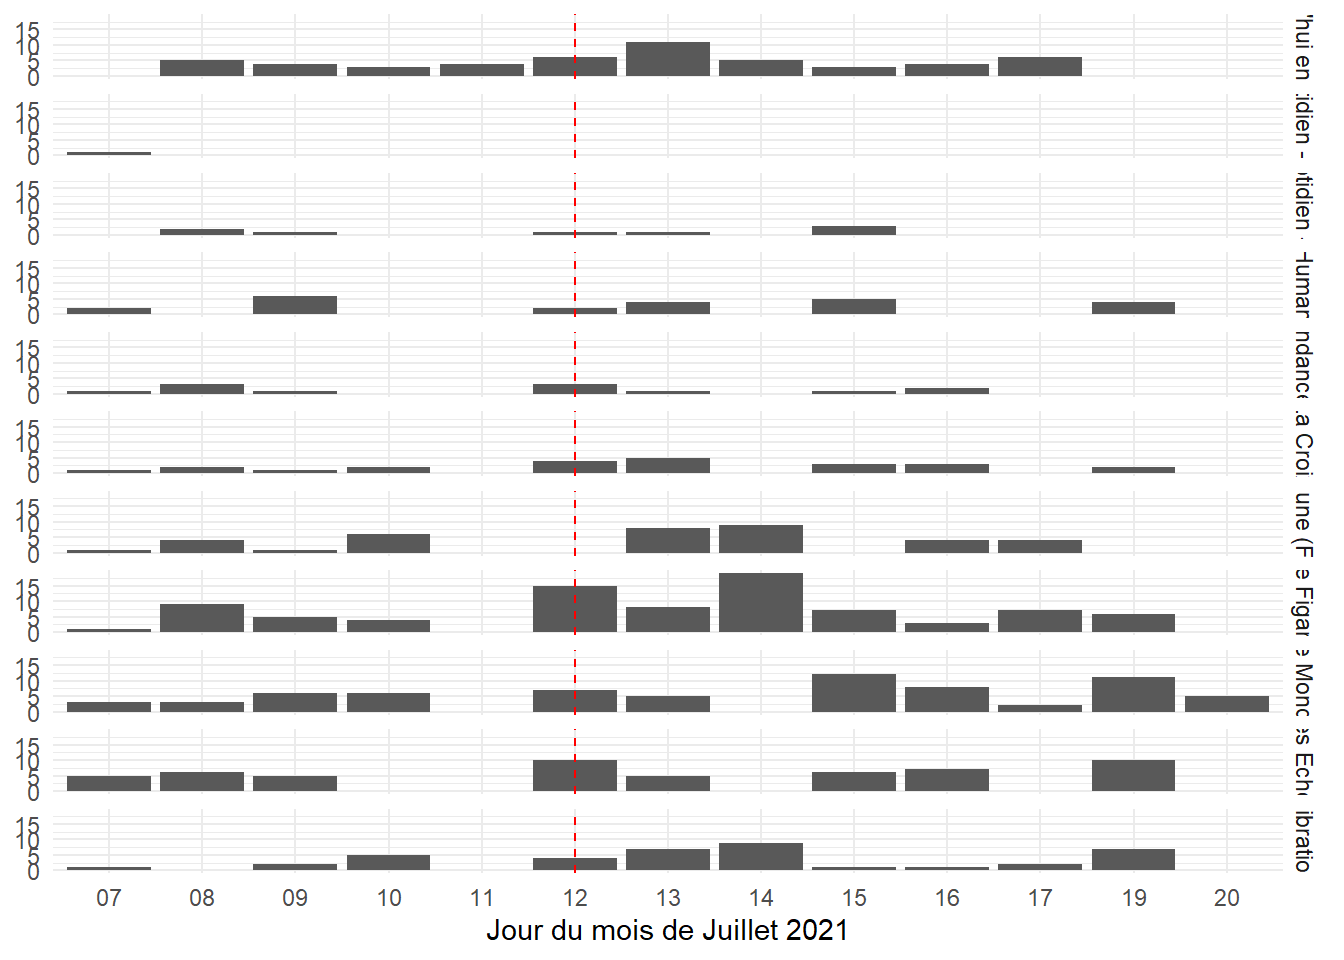
\includegraphics{q07_tokenisation_files/figure-pdf/unnamed-chunk-2-1.pdf}

On peut faire la même chose sur les mots, et en plus en éliminant les
\emph{stopwords}. l'intérêt de la procédure est de se concentrer sur les
idées, des paires de mots consistants du point de vue sémantique. Un
ordre ce dégage ! la bureaucratie est un moyen, puis une rationalité qui
dépend d'un exercice.

On note qu'il n'y a pas besoin de beaucoup de mots pour produire du sens
par l'analyse statistique de leurs distributions.

\begin{Shaded}
\begin{Highlighting}[]
\NormalTok{toc\_maxweber}\OtherTok{\textless{}{-}}\FunctionTok{tokenize\_ngrams}\NormalTok{(MaxWeber,}
                              \AttributeTok{n=}\DecValTok{3}\NormalTok{, }
                              \AttributeTok{n\_min=}\DecValTok{2}\NormalTok{, }
                              \AttributeTok{stopwords =} \FunctionTok{stopwords}\NormalTok{(}\StringTok{\textquotesingle{}fr\textquotesingle{}}\NormalTok{)) }\SpecialCharTok{\%\textgreater{}\%}
  \FunctionTok{as.data.frame}\NormalTok{()}\SpecialCharTok{\%\textgreater{}\%}
  \FunctionTok{rename}\NormalTok{(}\AttributeTok{tokens=}\DecValTok{1}\NormalTok{)}

\FunctionTok{qflextable}\NormalTok{(}\FunctionTok{head}\NormalTok{(toc\_maxweber, }\AttributeTok{n=}\DecValTok{19}\NormalTok{))}
\end{Highlighting}
\end{Shaded}

\global\setlength{\Oldarrayrulewidth}{\arrayrulewidth}

\global\setlength{\Oldtabcolsep}{\tabcolsep}

\setlength{\tabcolsep}{0pt}

\renewcommand*{\arraystretch}{1.5}



\providecommand{\ascline}[3]{\noalign{\global\arrayrulewidth #1}\arrayrulecolor[HTML]{#2}\cline{#3}}

\begin{longtable*}[c]{|p{1.98in}}



\hhline{>{\arrayrulecolor[HTML]{666666}\global\arrayrulewidth=1.5pt}-}

\multicolumn{1}{>{\cellcolor[HTML]{EFEFEF}\raggedright}m{\dimexpr 1.98in+0\tabcolsep}}{\textcolor[HTML]{000000}{\fontsize{10}{10}\selectfont{\textbf{tokens}}}} \\

\noalign{\global\arrayrulewidth 0pt}\arrayrulecolor[HTML]{000000}

\hhline{>{\arrayrulecolor[HTML]{666666}\global\arrayrulewidth=1.5pt}-}\endfirsthead 

\hhline{>{\arrayrulecolor[HTML]{666666}\global\arrayrulewidth=1.5pt}-}

\multicolumn{1}{>{\cellcolor[HTML]{EFEFEF}\raggedright}m{\dimexpr 1.98in+0\tabcolsep}}{\textcolor[HTML]{000000}{\fontsize{10}{10}\selectfont{\textbf{tokens}}}} \\

\noalign{\global\arrayrulewidth 0pt}\arrayrulecolor[HTML]{000000}

\hhline{>{\arrayrulecolor[HTML]{666666}\global\arrayrulewidth=1.5pt}-}\endhead



\multicolumn{1}{>{\cellcolor[HTML]{EFEFEF}\raggedright}m{\dimexpr 1.98in+0\tabcolsep}}{\textcolor[HTML]{000000}{\fontsize{10}{10}\selectfont{bureaucratie\ moyen}}} \\

\noalign{\global\arrayrulewidth 0pt}\arrayrulecolor[HTML]{000000}

\hhline{>{\arrayrulecolor[HTML]{666666}\global\arrayrulewidth=0.75pt}-}



\multicolumn{1}{>{\cellcolor[HTML]{EFEFEF}\raggedright}m{\dimexpr 1.98in+0\tabcolsep}}{\textcolor[HTML]{000000}{\fontsize{10}{10}\selectfont{bureaucratie\ moyen\ plus}}} \\

\noalign{\global\arrayrulewidth 0pt}\arrayrulecolor[HTML]{000000}

\hhline{>{\arrayrulecolor[HTML]{666666}\global\arrayrulewidth=0.75pt}-}



\multicolumn{1}{>{\cellcolor[HTML]{EFEFEF}\raggedright}m{\dimexpr 1.98in+0\tabcolsep}}{\textcolor[HTML]{000000}{\fontsize{10}{10}\selectfont{moyen\ plus}}} \\

\noalign{\global\arrayrulewidth 0pt}\arrayrulecolor[HTML]{000000}

\hhline{>{\arrayrulecolor[HTML]{666666}\global\arrayrulewidth=0.75pt}-}



\multicolumn{1}{>{\cellcolor[HTML]{EFEFEF}\raggedright}m{\dimexpr 1.98in+0\tabcolsep}}{\textcolor[HTML]{000000}{\fontsize{10}{10}\selectfont{moyen\ plus\ rationnel}}} \\

\noalign{\global\arrayrulewidth 0pt}\arrayrulecolor[HTML]{000000}

\hhline{>{\arrayrulecolor[HTML]{666666}\global\arrayrulewidth=0.75pt}-}



\multicolumn{1}{>{\cellcolor[HTML]{EFEFEF}\raggedright}m{\dimexpr 1.98in+0\tabcolsep}}{\textcolor[HTML]{000000}{\fontsize{10}{10}\selectfont{plus\ rationnel}}} \\

\noalign{\global\arrayrulewidth 0pt}\arrayrulecolor[HTML]{000000}

\hhline{>{\arrayrulecolor[HTML]{666666}\global\arrayrulewidth=0.75pt}-}



\multicolumn{1}{>{\cellcolor[HTML]{EFEFEF}\raggedright}m{\dimexpr 1.98in+0\tabcolsep}}{\textcolor[HTML]{000000}{\fontsize{10}{10}\selectfont{plus\ rationnel\ l’on}}} \\

\noalign{\global\arrayrulewidth 0pt}\arrayrulecolor[HTML]{000000}

\hhline{>{\arrayrulecolor[HTML]{666666}\global\arrayrulewidth=0.75pt}-}



\multicolumn{1}{>{\cellcolor[HTML]{EFEFEF}\raggedright}m{\dimexpr 1.98in+0\tabcolsep}}{\textcolor[HTML]{000000}{\fontsize{10}{10}\selectfont{rationnel\ l’on}}} \\

\noalign{\global\arrayrulewidth 0pt}\arrayrulecolor[HTML]{000000}

\hhline{>{\arrayrulecolor[HTML]{666666}\global\arrayrulewidth=0.75pt}-}



\multicolumn{1}{>{\cellcolor[HTML]{EFEFEF}\raggedright}m{\dimexpr 1.98in+0\tabcolsep}}{\textcolor[HTML]{000000}{\fontsize{10}{10}\selectfont{rationnel\ l’on\ connaisse}}} \\

\noalign{\global\arrayrulewidth 0pt}\arrayrulecolor[HTML]{000000}

\hhline{>{\arrayrulecolor[HTML]{666666}\global\arrayrulewidth=0.75pt}-}



\multicolumn{1}{>{\cellcolor[HTML]{EFEFEF}\raggedright}m{\dimexpr 1.98in+0\tabcolsep}}{\textcolor[HTML]{000000}{\fontsize{10}{10}\selectfont{l’on\ connaisse}}} \\

\noalign{\global\arrayrulewidth 0pt}\arrayrulecolor[HTML]{000000}

\hhline{>{\arrayrulecolor[HTML]{666666}\global\arrayrulewidth=0.75pt}-}



\multicolumn{1}{>{\cellcolor[HTML]{EFEFEF}\raggedright}m{\dimexpr 1.98in+0\tabcolsep}}{\textcolor[HTML]{000000}{\fontsize{10}{10}\selectfont{l’on\ connaisse\ exercer}}} \\

\noalign{\global\arrayrulewidth 0pt}\arrayrulecolor[HTML]{000000}

\hhline{>{\arrayrulecolor[HTML]{666666}\global\arrayrulewidth=0.75pt}-}



\multicolumn{1}{>{\cellcolor[HTML]{EFEFEF}\raggedright}m{\dimexpr 1.98in+0\tabcolsep}}{\textcolor[HTML]{000000}{\fontsize{10}{10}\selectfont{connaisse\ exercer}}} \\

\noalign{\global\arrayrulewidth 0pt}\arrayrulecolor[HTML]{000000}

\hhline{>{\arrayrulecolor[HTML]{666666}\global\arrayrulewidth=0.75pt}-}



\multicolumn{1}{>{\cellcolor[HTML]{EFEFEF}\raggedright}m{\dimexpr 1.98in+0\tabcolsep}}{\textcolor[HTML]{000000}{\fontsize{10}{10}\selectfont{connaisse\ exercer\ contrôle}}} \\

\noalign{\global\arrayrulewidth 0pt}\arrayrulecolor[HTML]{000000}

\hhline{>{\arrayrulecolor[HTML]{666666}\global\arrayrulewidth=0.75pt}-}



\multicolumn{1}{>{\cellcolor[HTML]{EFEFEF}\raggedright}m{\dimexpr 1.98in+0\tabcolsep}}{\textcolor[HTML]{000000}{\fontsize{10}{10}\selectfont{exercer\ contrôle}}} \\

\noalign{\global\arrayrulewidth 0pt}\arrayrulecolor[HTML]{000000}

\hhline{>{\arrayrulecolor[HTML]{666666}\global\arrayrulewidth=0.75pt}-}



\multicolumn{1}{>{\cellcolor[HTML]{EFEFEF}\raggedright}m{\dimexpr 1.98in+0\tabcolsep}}{\textcolor[HTML]{000000}{\fontsize{10}{10}\selectfont{exercer\ contrôle\ impératif}}} \\

\noalign{\global\arrayrulewidth 0pt}\arrayrulecolor[HTML]{000000}

\hhline{>{\arrayrulecolor[HTML]{666666}\global\arrayrulewidth=0.75pt}-}



\multicolumn{1}{>{\cellcolor[HTML]{EFEFEF}\raggedright}m{\dimexpr 1.98in+0\tabcolsep}}{\textcolor[HTML]{000000}{\fontsize{10}{10}\selectfont{contrôle\ impératif}}} \\

\noalign{\global\arrayrulewidth 0pt}\arrayrulecolor[HTML]{000000}

\hhline{>{\arrayrulecolor[HTML]{666666}\global\arrayrulewidth=0.75pt}-}



\multicolumn{1}{>{\cellcolor[HTML]{EFEFEF}\raggedright}m{\dimexpr 1.98in+0\tabcolsep}}{\textcolor[HTML]{000000}{\fontsize{10}{10}\selectfont{contrôle\ impératif\ êtres}}} \\

\noalign{\global\arrayrulewidth 0pt}\arrayrulecolor[HTML]{000000}

\hhline{>{\arrayrulecolor[HTML]{666666}\global\arrayrulewidth=0.75pt}-}



\multicolumn{1}{>{\cellcolor[HTML]{EFEFEF}\raggedright}m{\dimexpr 1.98in+0\tabcolsep}}{\textcolor[HTML]{000000}{\fontsize{10}{10}\selectfont{impératif\ êtres}}} \\

\noalign{\global\arrayrulewidth 0pt}\arrayrulecolor[HTML]{000000}

\hhline{>{\arrayrulecolor[HTML]{666666}\global\arrayrulewidth=0.75pt}-}



\multicolumn{1}{>{\cellcolor[HTML]{EFEFEF}\raggedright}m{\dimexpr 1.98in+0\tabcolsep}}{\textcolor[HTML]{000000}{\fontsize{10}{10}\selectfont{impératif\ êtres\ humains}}} \\

\noalign{\global\arrayrulewidth 0pt}\arrayrulecolor[HTML]{000000}

\hhline{>{\arrayrulecolor[HTML]{666666}\global\arrayrulewidth=0.75pt}-}



\multicolumn{1}{>{\cellcolor[HTML]{EFEFEF}\raggedright}m{\dimexpr 1.98in+0\tabcolsep}}{\textcolor[HTML]{000000}{\fontsize{10}{10}\selectfont{êtres\ humains}}} \\

\noalign{\global\arrayrulewidth 0pt}\arrayrulecolor[HTML]{000000}

\hhline{>{\arrayrulecolor[HTML]{666666}\global\arrayrulewidth=1.5pt}-}



\end{longtable*}



\arrayrulecolor[HTML]{000000}

\global\setlength{\arrayrulewidth}{\Oldarrayrulewidth}

\global\setlength{\tabcolsep}{\Oldtabcolsep}

\renewcommand*{\arraystretch}{1}

On peut également s'intéresser aux n-grammes non directement consécutifs
mais séparés par k \emph{tokens}. C'est sans doute un moyen de saisir
des corrélations de mots à plus grande distance. La possibilité formelle
est là , nous avouons ne pas savoir à quel usage elle correspond. Nous
serions sur ce point ravi d'avoir des réponses.

\begin{Shaded}
\begin{Highlighting}[]
\NormalTok{toc\_maxweber}\OtherTok{\textless{}{-}}\FunctionTok{tokenize\_skip\_ngrams}\NormalTok{(MaxWeber,}
                                   \AttributeTok{n=}\DecValTok{3}\NormalTok{, }
                                   \AttributeTok{n\_min=}\DecValTok{2}\NormalTok{, }
                                   \AttributeTok{k=}\DecValTok{2}\NormalTok{, }
                                   \AttributeTok{stopwords =} \FunctionTok{stopwords}\NormalTok{(}\StringTok{\textquotesingle{}fr\textquotesingle{}}\NormalTok{)) }\SpecialCharTok{\%\textgreater{}\%}
        \FunctionTok{as.data.frame}\NormalTok{()}\SpecialCharTok{\%\textgreater{}\%}\FunctionTok{rename}\NormalTok{(}\AttributeTok{tokens=}\DecValTok{1}\NormalTok{)}
\FunctionTok{qflextable}\NormalTok{(}\FunctionTok{head}\NormalTok{(toc\_maxweber, }\AttributeTok{n=}\DecValTok{19}\NormalTok{))}
\end{Highlighting}
\end{Shaded}

\global\setlength{\Oldarrayrulewidth}{\arrayrulewidth}

\global\setlength{\Oldtabcolsep}{\tabcolsep}

\setlength{\tabcolsep}{0pt}

\renewcommand*{\arraystretch}{1.5}



\providecommand{\ascline}[3]{\noalign{\global\arrayrulewidth #1}\arrayrulecolor[HTML]{#2}\cline{#3}}

\begin{longtable*}[c]{|p{2.33in}}



\hhline{>{\arrayrulecolor[HTML]{666666}\global\arrayrulewidth=1.5pt}-}

\multicolumn{1}{>{\cellcolor[HTML]{EFEFEF}\raggedright}m{\dimexpr 2.33in+0\tabcolsep}}{\textcolor[HTML]{000000}{\fontsize{10}{10}\selectfont{\textbf{tokens}}}} \\

\noalign{\global\arrayrulewidth 0pt}\arrayrulecolor[HTML]{000000}

\hhline{>{\arrayrulecolor[HTML]{666666}\global\arrayrulewidth=1.5pt}-}\endfirsthead 

\hhline{>{\arrayrulecolor[HTML]{666666}\global\arrayrulewidth=1.5pt}-}

\multicolumn{1}{>{\cellcolor[HTML]{EFEFEF}\raggedright}m{\dimexpr 2.33in+0\tabcolsep}}{\textcolor[HTML]{000000}{\fontsize{10}{10}\selectfont{\textbf{tokens}}}} \\

\noalign{\global\arrayrulewidth 0pt}\arrayrulecolor[HTML]{000000}

\hhline{>{\arrayrulecolor[HTML]{666666}\global\arrayrulewidth=1.5pt}-}\endhead



\multicolumn{1}{>{\cellcolor[HTML]{EFEFEF}\raggedright}m{\dimexpr 2.33in+0\tabcolsep}}{\textcolor[HTML]{000000}{\fontsize{10}{10}\selectfont{bureaucratie\ moyen}}} \\

\noalign{\global\arrayrulewidth 0pt}\arrayrulecolor[HTML]{000000}

\hhline{>{\arrayrulecolor[HTML]{666666}\global\arrayrulewidth=0.75pt}-}



\multicolumn{1}{>{\cellcolor[HTML]{EFEFEF}\raggedright}m{\dimexpr 2.33in+0\tabcolsep}}{\textcolor[HTML]{000000}{\fontsize{10}{10}\selectfont{bureaucratie\ plus}}} \\

\noalign{\global\arrayrulewidth 0pt}\arrayrulecolor[HTML]{000000}

\hhline{>{\arrayrulecolor[HTML]{666666}\global\arrayrulewidth=0.75pt}-}



\multicolumn{1}{>{\cellcolor[HTML]{EFEFEF}\raggedright}m{\dimexpr 2.33in+0\tabcolsep}}{\textcolor[HTML]{000000}{\fontsize{10}{10}\selectfont{bureaucratie\ rationnel}}} \\

\noalign{\global\arrayrulewidth 0pt}\arrayrulecolor[HTML]{000000}

\hhline{>{\arrayrulecolor[HTML]{666666}\global\arrayrulewidth=0.75pt}-}



\multicolumn{1}{>{\cellcolor[HTML]{EFEFEF}\raggedright}m{\dimexpr 2.33in+0\tabcolsep}}{\textcolor[HTML]{000000}{\fontsize{10}{10}\selectfont{bureaucratie\ moyen\ plus}}} \\

\noalign{\global\arrayrulewidth 0pt}\arrayrulecolor[HTML]{000000}

\hhline{>{\arrayrulecolor[HTML]{666666}\global\arrayrulewidth=0.75pt}-}



\multicolumn{1}{>{\cellcolor[HTML]{EFEFEF}\raggedright}m{\dimexpr 2.33in+0\tabcolsep}}{\textcolor[HTML]{000000}{\fontsize{10}{10}\selectfont{bureaucratie\ moyen\ rationnel}}} \\

\noalign{\global\arrayrulewidth 0pt}\arrayrulecolor[HTML]{000000}

\hhline{>{\arrayrulecolor[HTML]{666666}\global\arrayrulewidth=0.75pt}-}



\multicolumn{1}{>{\cellcolor[HTML]{EFEFEF}\raggedright}m{\dimexpr 2.33in+0\tabcolsep}}{\textcolor[HTML]{000000}{\fontsize{10}{10}\selectfont{bureaucratie\ moyen\ l’on}}} \\

\noalign{\global\arrayrulewidth 0pt}\arrayrulecolor[HTML]{000000}

\hhline{>{\arrayrulecolor[HTML]{666666}\global\arrayrulewidth=0.75pt}-}



\multicolumn{1}{>{\cellcolor[HTML]{EFEFEF}\raggedright}m{\dimexpr 2.33in+0\tabcolsep}}{\textcolor[HTML]{000000}{\fontsize{10}{10}\selectfont{bureaucratie\ plus\ rationnel}}} \\

\noalign{\global\arrayrulewidth 0pt}\arrayrulecolor[HTML]{000000}

\hhline{>{\arrayrulecolor[HTML]{666666}\global\arrayrulewidth=0.75pt}-}



\multicolumn{1}{>{\cellcolor[HTML]{EFEFEF}\raggedright}m{\dimexpr 2.33in+0\tabcolsep}}{\textcolor[HTML]{000000}{\fontsize{10}{10}\selectfont{bureaucratie\ plus\ l’on}}} \\

\noalign{\global\arrayrulewidth 0pt}\arrayrulecolor[HTML]{000000}

\hhline{>{\arrayrulecolor[HTML]{666666}\global\arrayrulewidth=0.75pt}-}



\multicolumn{1}{>{\cellcolor[HTML]{EFEFEF}\raggedright}m{\dimexpr 2.33in+0\tabcolsep}}{\textcolor[HTML]{000000}{\fontsize{10}{10}\selectfont{bureaucratie\ plus\ connaisse}}} \\

\noalign{\global\arrayrulewidth 0pt}\arrayrulecolor[HTML]{000000}

\hhline{>{\arrayrulecolor[HTML]{666666}\global\arrayrulewidth=0.75pt}-}



\multicolumn{1}{>{\cellcolor[HTML]{EFEFEF}\raggedright}m{\dimexpr 2.33in+0\tabcolsep}}{\textcolor[HTML]{000000}{\fontsize{10}{10}\selectfont{bureaucratie\ rationnel\ l’on}}} \\

\noalign{\global\arrayrulewidth 0pt}\arrayrulecolor[HTML]{000000}

\hhline{>{\arrayrulecolor[HTML]{666666}\global\arrayrulewidth=0.75pt}-}



\multicolumn{1}{>{\cellcolor[HTML]{EFEFEF}\raggedright}m{\dimexpr 2.33in+0\tabcolsep}}{\textcolor[HTML]{000000}{\fontsize{10}{10}\selectfont{bureaucratie\ rationnel\ connaisse}}} \\

\noalign{\global\arrayrulewidth 0pt}\arrayrulecolor[HTML]{000000}

\hhline{>{\arrayrulecolor[HTML]{666666}\global\arrayrulewidth=0.75pt}-}



\multicolumn{1}{>{\cellcolor[HTML]{EFEFEF}\raggedright}m{\dimexpr 2.33in+0\tabcolsep}}{\textcolor[HTML]{000000}{\fontsize{10}{10}\selectfont{bureaucratie\ rationnel\ exercer}}} \\

\noalign{\global\arrayrulewidth 0pt}\arrayrulecolor[HTML]{000000}

\hhline{>{\arrayrulecolor[HTML]{666666}\global\arrayrulewidth=0.75pt}-}



\multicolumn{1}{>{\cellcolor[HTML]{EFEFEF}\raggedright}m{\dimexpr 2.33in+0\tabcolsep}}{\textcolor[HTML]{000000}{\fontsize{10}{10}\selectfont{moyen\ plus}}} \\

\noalign{\global\arrayrulewidth 0pt}\arrayrulecolor[HTML]{000000}

\hhline{>{\arrayrulecolor[HTML]{666666}\global\arrayrulewidth=0.75pt}-}



\multicolumn{1}{>{\cellcolor[HTML]{EFEFEF}\raggedright}m{\dimexpr 2.33in+0\tabcolsep}}{\textcolor[HTML]{000000}{\fontsize{10}{10}\selectfont{moyen\ rationnel}}} \\

\noalign{\global\arrayrulewidth 0pt}\arrayrulecolor[HTML]{000000}

\hhline{>{\arrayrulecolor[HTML]{666666}\global\arrayrulewidth=0.75pt}-}



\multicolumn{1}{>{\cellcolor[HTML]{EFEFEF}\raggedright}m{\dimexpr 2.33in+0\tabcolsep}}{\textcolor[HTML]{000000}{\fontsize{10}{10}\selectfont{moyen\ l’on}}} \\

\noalign{\global\arrayrulewidth 0pt}\arrayrulecolor[HTML]{000000}

\hhline{>{\arrayrulecolor[HTML]{666666}\global\arrayrulewidth=0.75pt}-}



\multicolumn{1}{>{\cellcolor[HTML]{EFEFEF}\raggedright}m{\dimexpr 2.33in+0\tabcolsep}}{\textcolor[HTML]{000000}{\fontsize{10}{10}\selectfont{moyen\ plus\ rationnel}}} \\

\noalign{\global\arrayrulewidth 0pt}\arrayrulecolor[HTML]{000000}

\hhline{>{\arrayrulecolor[HTML]{666666}\global\arrayrulewidth=0.75pt}-}



\multicolumn{1}{>{\cellcolor[HTML]{EFEFEF}\raggedright}m{\dimexpr 2.33in+0\tabcolsep}}{\textcolor[HTML]{000000}{\fontsize{10}{10}\selectfont{moyen\ plus\ l’on}}} \\

\noalign{\global\arrayrulewidth 0pt}\arrayrulecolor[HTML]{000000}

\hhline{>{\arrayrulecolor[HTML]{666666}\global\arrayrulewidth=0.75pt}-}



\multicolumn{1}{>{\cellcolor[HTML]{EFEFEF}\raggedright}m{\dimexpr 2.33in+0\tabcolsep}}{\textcolor[HTML]{000000}{\fontsize{10}{10}\selectfont{moyen\ plus\ connaisse}}} \\

\noalign{\global\arrayrulewidth 0pt}\arrayrulecolor[HTML]{000000}

\hhline{>{\arrayrulecolor[HTML]{666666}\global\arrayrulewidth=0.75pt}-}



\multicolumn{1}{>{\cellcolor[HTML]{EFEFEF}\raggedright}m{\dimexpr 2.33in+0\tabcolsep}}{\textcolor[HTML]{000000}{\fontsize{10}{10}\selectfont{moyen\ rationnel\ l’on}}} \\

\noalign{\global\arrayrulewidth 0pt}\arrayrulecolor[HTML]{000000}

\hhline{>{\arrayrulecolor[HTML]{666666}\global\arrayrulewidth=1.5pt}-}



\end{longtable*}



\arrayrulecolor[HTML]{000000}

\global\setlength{\arrayrulewidth}{\Oldarrayrulewidth}

\global\setlength{\tabcolsep}{\Oldtabcolsep}

\renewcommand*{\arraystretch}{1}

Dans cet exemple, aucun n-gramme n'est répété, mais c'est rarement le
cas avec des corpus plus importants. Dans ce cas, une forte répétition
de n-grammes est un indice d'une unité sémantique composée de plusieurs
\emph{tokens} que l'on peut alors regrouper en un seul et même
\emph{token}. C'est ce que l'on verra dans la section suivante, avec la
méthodes des collocation,

\section{Choisir des n-grammes
pertinents}\label{choisir-des-n-grammes-pertinents}

Dans ce e-book l'unité principale d'analyse restera le mot. Mais nous
savons, au moins intuitivement que certaines combinaisons de mots
représentent des expressions qui ont la valeur d'un mot, une valeur
sémantique, par exemple, l'expression ``Assemblée Nationale''. Ces deux
mots réunis constituent un syntagme, une unité de sens. La question qui
se pose est alors de savoir comment les identifier dans le flot des
n-grammes ?

La technique est simple : si deux mots se retrouvent dans un ordre donné
plus fréquemment que ce que le produit de leurs probabilités
d'apparition laisse espérer, c'est qu'ils constituent une expression. On
peut imaginer faire un test du chi² pour décider si un couple de mots
constitue une unité sémantique ou non.

Le package quanteda propose une bonne solution à ce problème avec la
fonction collocation.

\subsection{\texorpdfstring{Créer les \emph{tokens} avec
`quanteda'}{Créer les tokens avec `quanteda'}}\label{cruxe9er-les-tokens-avec-quanteda}

À partir du corpus des commentaires de TripAdvisor concernant les hôtels
de Polynésie Française,

\begin{Shaded}
\begin{Highlighting}[]
\CommentTok{\#les données}
\NormalTok{AvisTripadvisor}\OtherTok{\textless{}{-}}\FunctionTok{read\_rds}\NormalTok{(}\StringTok{"./data/AvisTripadvisor.rds"}\NormalTok{)}
\NormalTok{AvisTripadvisor}\SpecialCharTok{$}\NormalTok{Taille\_hotel}\OtherTok{\textless{}{-}}\FunctionTok{as.character}\NormalTok{(AvisTripadvisor}\SpecialCharTok{$}\NormalTok{Taille\_hotel)}
\NormalTok{AvisTripadvisor}\SpecialCharTok{$}\NormalTok{Taille\_hotel[}\FunctionTok{is.na}\NormalTok{(AvisTripadvisor}\SpecialCharTok{$}\NormalTok{Taille\_hotel)]}\OtherTok{\textless{}{-}}\StringTok{"Autre"}


\CommentTok{\#création du corpus}
\NormalTok{corpus}\OtherTok{\textless{}{-}}\FunctionTok{corpus}\NormalTok{(AvisTripadvisor,}\AttributeTok{docid\_field =} \StringTok{"ID"}\NormalTok{,}\AttributeTok{text\_field =} \StringTok{"Commetaire"}\NormalTok{, }\AttributeTok{docvars =}\NormalTok{AvisTripadvisor)}
\NormalTok{ft}\OtherTok{\textless{}{-}} \FunctionTok{head}\NormalTok{(corpus,}\DecValTok{3}\NormalTok{) }\SpecialCharTok{\%\textgreater{}\%} \FunctionTok{as.data.frame}\NormalTok{()}\SpecialCharTok{\%\textgreater{}\%}
  \FunctionTok{rename}\NormalTok{(}\AttributeTok{tokens=}\DecValTok{1}\NormalTok{)}\SpecialCharTok{\%\textgreater{}\%}
  \FunctionTok{flextable}\NormalTok{(}\AttributeTok{cwidth =} \DecValTok{6}\NormalTok{)}
\NormalTok{ft}
\end{Highlighting}
\end{Shaded}

\global\setlength{\Oldarrayrulewidth}{\arrayrulewidth}

\global\setlength{\Oldtabcolsep}{\tabcolsep}

\setlength{\tabcolsep}{0pt}

\renewcommand*{\arraystretch}{1.5}



\providecommand{\ascline}[3]{\noalign{\global\arrayrulewidth #1}\arrayrulecolor[HTML]{#2}\cline{#3}}

\begin{longtable}[c]{|p{6.00in}}
\caption{corpus}\tabularnewline




\hhline{>{\arrayrulecolor[HTML]{666666}\global\arrayrulewidth=1.5pt}-}

\multicolumn{1}{>{\cellcolor[HTML]{EFEFEF}\raggedright}m{\dimexpr 6in+0\tabcolsep}}{\textcolor[HTML]{000000}{\fontsize{10}{10}\selectfont{\textbf{tokens}}}} \\

\noalign{\global\arrayrulewidth 0pt}\arrayrulecolor[HTML]{000000}

\hhline{>{\arrayrulecolor[HTML]{666666}\global\arrayrulewidth=1.5pt}-}\endfirsthead 

\hhline{>{\arrayrulecolor[HTML]{666666}\global\arrayrulewidth=1.5pt}-}

\multicolumn{1}{>{\cellcolor[HTML]{EFEFEF}\raggedright}m{\dimexpr 6in+0\tabcolsep}}{\textcolor[HTML]{000000}{\fontsize{10}{10}\selectfont{\textbf{tokens}}}} \\

\noalign{\global\arrayrulewidth 0pt}\arrayrulecolor[HTML]{000000}

\hhline{>{\arrayrulecolor[HTML]{666666}\global\arrayrulewidth=1.5pt}-}\endhead



\multicolumn{1}{>{\cellcolor[HTML]{EFEFEF}\raggedright}m{\dimexpr 6in+0\tabcolsep}}{\textcolor[HTML]{000000}{\fontsize{10}{10}\selectfont{Tout\ est\ magnifique\ au\ Vahine\ island.\ Séjour\ de\ rêve\ avec\ une\ équipe\ très\ chaleureuse\ .\ Le\ cadre\ est\ splendide.\ Notre\ meilleur\ hébergement\ en\ Polynésie.Merci\ à\ toute\ l'\ équipe\ pour\ votre\ gentillesse\ et\ vos\ nombreuses\ attentions.}}} \\

\noalign{\global\arrayrulewidth 0pt}\arrayrulecolor[HTML]{000000}

\hhline{>{\arrayrulecolor[HTML]{666666}\global\arrayrulewidth=0.75pt}-}



\multicolumn{1}{>{\cellcolor[HTML]{EFEFEF}\raggedright}m{\dimexpr 6in+0\tabcolsep}}{\textcolor[HTML]{000000}{\fontsize{10}{10}\selectfont{Tout\ était\ parfait,\ notre\ meilleure\ expérience\ et\ plus\ belle\ découverte\ en\ Polynésie.Un\ grand\ merci\ à\ Amélie\ et\ toute\ son\ équipe\ pour\ un\ service\ de\ très\ haut\ niveau.De\ la\ chambre,\ en\ passant\ par\ la\ restauration\ et\ les\ activités,\ tout\ était\ parfait.\ Encore\ merci\ à\ tous,\ en\ espérant\ revenir\ très\ vite.}}} \\

\noalign{\global\arrayrulewidth 0pt}\arrayrulecolor[HTML]{000000}

\hhline{>{\arrayrulecolor[HTML]{666666}\global\arrayrulewidth=0.75pt}-}



\multicolumn{1}{>{\cellcolor[HTML]{EFEFEF}\raggedright}m{\dimexpr 6in+0\tabcolsep}}{\textcolor[HTML]{000000}{\fontsize{10}{10}\selectfont{Un\ séjour\ magnifique,\ 3\ jours\ époustouflants,\ accueillis\ chaleureusement\ par\ toute\ l’équipe\ du\ Vahine\ Island.\ Tout\ est\ au\ rendez\ vous,\ la\ cuisine\ délicieuse,\ le\ lieu\ au\ delà\ de\ notre\ imagination,\ un\ calme\ parfait.\ À\ faire,\ re\ faire,\ sans\ jamais\ s’en\ lasser.}}} \\

\noalign{\global\arrayrulewidth 0pt}\arrayrulecolor[HTML]{000000}

\hhline{>{\arrayrulecolor[HTML]{666666}\global\arrayrulewidth=1.5pt}-}



\end{longtable}



\arrayrulecolor[HTML]{000000}

\global\setlength{\arrayrulewidth}{\Oldarrayrulewidth}

\global\setlength{\tabcolsep}{\Oldtabcolsep}

\renewcommand*{\arraystretch}{1}

On crée un objet de format \emph{token}, avec la fonction tokens de
quanteda, et on choisit d'enlèver la ponctuation, les symboles et les
nombres avec les arguments correspondants.

Notre tokenizer ici a quelques problèmes . Si le ``.'' n'est pas suivi
d'un espace, il ne peut distinguer les mots, il ne saisit pas non plus
l'ellipse de ``l'équipe'', qui devrait distinguer le determinant ``la''
de ``équipe. Souvent il faudra au préalable remanier les chaines de
caractère pour une meilleure qualité de tokenisation.

\begin{Shaded}
\begin{Highlighting}[]
\CommentTok{\#transformation en objet token}
\NormalTok{tok}\OtherTok{\textless{}{-}}\FunctionTok{tokens}\NormalTok{(corpus,}\AttributeTok{remove\_punct =} \ConstantTok{TRUE}\NormalTok{, }\AttributeTok{remove\_symbols=}\ConstantTok{TRUE}\NormalTok{, }\AttributeTok{remove\_numbers=}\ConstantTok{TRUE}\NormalTok{)}

\FunctionTok{head}\NormalTok{(tok,}\DecValTok{3}\NormalTok{) }
\end{Highlighting}
\end{Shaded}

\begin{verbatim}
Tokens consisting of 3 documents and 21 docvars.
1 :
 [1] "Tout"       "est"        "magnifique" "au"         "Vahine"    
 [6] "island"     "Séjour"     "de"         "rêve"       "avec"      
[11] "une"        "équipe"    
[ ... and 22 more ]

2 :
 [1] "Tout"         "était"        "parfait"      "notre"        "meilleure"   
 [6] "expérience"   "et"           "plus"         "belle"        "découverte"  
[11] "en"           "Polynésie.Un"
[ ... and 37 more ]

3 :
 [1] "Un"              "séjour"          "magnifique"      "jours"          
 [5] "époustouflants"  "accueillis"      "chaleureusement" "par"            
 [9] "toute"           "l’équipe"        "du"              "Vahine"         
[ ... and 27 more ]
\end{verbatim}

Au passage, on peut aussi enlever les \emph{stopwords}. C'est a dire les
mots d'usages courants mais sans signification intrinsèque : les
conjonctions, les déterminants, etc, qui se présentent sous la formes de
dictionnaires.

Pour que les n-grammes très fréquents restent des syntagmes signifiants,
on laisse apparentes les positions des \emph{stopwords}, avec l'option
\texttt{padding=\ TRUE}.

\begin{Shaded}
\begin{Highlighting}[]
\CommentTok{\#enlever les stopwords}
\NormalTok{tok}\OtherTok{\textless{}{-}}\FunctionTok{tokens\_remove}\NormalTok{(tok,}\FunctionTok{stopwords}\NormalTok{(}\StringTok{\textquotesingle{}fr\textquotesingle{}}\NormalTok{),}\AttributeTok{padding=}\ConstantTok{FALSE}\NormalTok{)}
\FunctionTok{head}\NormalTok{(tok, }\DecValTok{3}\NormalTok{)}
\end{Highlighting}
\end{Shaded}

\begin{verbatim}
Tokens consisting of 3 documents and 21 docvars.
1 :
 [1] "Tout"        "magnifique"  "Vahine"      "island"      "Séjour"     
 [6] "rêve"        "équipe"      "très"        "chaleureuse" "cadre"      
[11] "splendide"   "meilleur"   
[ ... and 7 more ]

2 :
 [1] "Tout"         "parfait"      "meilleure"    "expérience"   "plus"        
 [6] "belle"        "découverte"   "Polynésie.Un" "grand"        "merci"       
[11] "Amélie"       "toute"       
[ ... and 18 more ]

3 :
 [1] "séjour"          "magnifique"      "jours"           "époustouflants" 
 [5] "accueillis"      "chaleureusement" "toute"           "l’équipe"       
 [9] "Vahine"          "Island"          "Tout"            "rendez"         
[ ... and 13 more ]
\end{verbatim}

\subsection{Application à la détection des entités
nommées}\label{application-uxe0-la-duxe9tection-des-entituxe9s-nommuxe9es}

On cherche ici à identifier les noms propres présents dans le corpus.

\begin{Shaded}
\begin{Highlighting}[]
\FunctionTok{library}\NormalTok{(quanteda.textstats)}
\CommentTok{\#on sélectionne les mots commençant par une majuscule}
\NormalTok{toks\_cap }\OtherTok{\textless{}{-}} \FunctionTok{tokens\_select}\NormalTok{(tok, }
                               \AttributeTok{pattern =} \StringTok{"\^{}[A{-}Z]"}\NormalTok{,}
                               \AttributeTok{valuetype =} \StringTok{"regex"}\NormalTok{,}
                               \AttributeTok{case\_insensitive =} \ConstantTok{FALSE}\NormalTok{, }
                               \AttributeTok{padding =} \ConstantTok{TRUE}\NormalTok{)}

\CommentTok{\#on cherche les collocations}
\NormalTok{tstat\_col\_cap }\OtherTok{\textless{}{-}} \FunctionTok{textstat\_collocations}\NormalTok{(toks\_cap, }\AttributeTok{min\_count =} \DecValTok{3}\NormalTok{, }\AttributeTok{tolower =} \ConstantTok{FALSE}\NormalTok{)}

\FunctionTok{flextable}\NormalTok{(}\FunctionTok{head}\NormalTok{(}\FunctionTok{as.data.frame}\NormalTok{(tstat\_col\_cap)))}
\end{Highlighting}
\end{Shaded}

\global\setlength{\Oldarrayrulewidth}{\arrayrulewidth}

\global\setlength{\Oldtabcolsep}{\tabcolsep}

\setlength{\tabcolsep}{0pt}

\renewcommand*{\arraystretch}{1.5}



\providecommand{\ascline}[3]{\noalign{\global\arrayrulewidth #1}\arrayrulecolor[HTML]{#2}\cline{#3}}

\begin{longtable*}[c]{|p{0.75in}|p{0.75in}|p{0.75in}|p{0.75in}|p{0.75in}|p{0.75in}}



\hhline{>{\arrayrulecolor[HTML]{666666}\global\arrayrulewidth=1.5pt}->{\arrayrulecolor[HTML]{666666}\global\arrayrulewidth=1.5pt}->{\arrayrulecolor[HTML]{666666}\global\arrayrulewidth=1.5pt}->{\arrayrulecolor[HTML]{666666}\global\arrayrulewidth=1.5pt}->{\arrayrulecolor[HTML]{666666}\global\arrayrulewidth=1.5pt}->{\arrayrulecolor[HTML]{666666}\global\arrayrulewidth=1.5pt}-}

\multicolumn{1}{>{\cellcolor[HTML]{EFEFEF}\raggedright}m{\dimexpr 0.75in+0\tabcolsep}}{\textcolor[HTML]{000000}{\fontsize{10}{10}\selectfont{\textbf{collocation}}}} & \multicolumn{1}{>{\cellcolor[HTML]{EFEFEF}\raggedleft}m{\dimexpr 0.75in+0\tabcolsep}}{\textcolor[HTML]{000000}{\fontsize{10}{10}\selectfont{\textbf{count}}}} & \multicolumn{1}{>{\cellcolor[HTML]{EFEFEF}\raggedleft}m{\dimexpr 0.75in+0\tabcolsep}}{\textcolor[HTML]{000000}{\fontsize{10}{10}\selectfont{\textbf{count\_nested}}}} & \multicolumn{1}{>{\cellcolor[HTML]{EFEFEF}\raggedleft}m{\dimexpr 0.75in+0\tabcolsep}}{\textcolor[HTML]{000000}{\fontsize{10}{10}\selectfont{\textbf{length}}}} & \multicolumn{1}{>{\cellcolor[HTML]{EFEFEF}\raggedleft}m{\dimexpr 0.75in+0\tabcolsep}}{\textcolor[HTML]{000000}{\fontsize{10}{10}\selectfont{\textbf{lambda}}}} & \multicolumn{1}{>{\cellcolor[HTML]{EFEFEF}\raggedleft}m{\dimexpr 0.75in+0\tabcolsep}}{\textcolor[HTML]{000000}{\fontsize{10}{10}\selectfont{\textbf{z}}}} \\

\noalign{\global\arrayrulewidth 0pt}\arrayrulecolor[HTML]{000000}

\hhline{>{\arrayrulecolor[HTML]{666666}\global\arrayrulewidth=1.5pt}->{\arrayrulecolor[HTML]{666666}\global\arrayrulewidth=1.5pt}->{\arrayrulecolor[HTML]{666666}\global\arrayrulewidth=1.5pt}->{\arrayrulecolor[HTML]{666666}\global\arrayrulewidth=1.5pt}->{\arrayrulecolor[HTML]{666666}\global\arrayrulewidth=1.5pt}->{\arrayrulecolor[HTML]{666666}\global\arrayrulewidth=1.5pt}-}\endfirsthead 

\hhline{>{\arrayrulecolor[HTML]{666666}\global\arrayrulewidth=1.5pt}->{\arrayrulecolor[HTML]{666666}\global\arrayrulewidth=1.5pt}->{\arrayrulecolor[HTML]{666666}\global\arrayrulewidth=1.5pt}->{\arrayrulecolor[HTML]{666666}\global\arrayrulewidth=1.5pt}->{\arrayrulecolor[HTML]{666666}\global\arrayrulewidth=1.5pt}->{\arrayrulecolor[HTML]{666666}\global\arrayrulewidth=1.5pt}-}

\multicolumn{1}{>{\cellcolor[HTML]{EFEFEF}\raggedright}m{\dimexpr 0.75in+0\tabcolsep}}{\textcolor[HTML]{000000}{\fontsize{10}{10}\selectfont{\textbf{collocation}}}} & \multicolumn{1}{>{\cellcolor[HTML]{EFEFEF}\raggedleft}m{\dimexpr 0.75in+0\tabcolsep}}{\textcolor[HTML]{000000}{\fontsize{10}{10}\selectfont{\textbf{count}}}} & \multicolumn{1}{>{\cellcolor[HTML]{EFEFEF}\raggedleft}m{\dimexpr 0.75in+0\tabcolsep}}{\textcolor[HTML]{000000}{\fontsize{10}{10}\selectfont{\textbf{count\_nested}}}} & \multicolumn{1}{>{\cellcolor[HTML]{EFEFEF}\raggedleft}m{\dimexpr 0.75in+0\tabcolsep}}{\textcolor[HTML]{000000}{\fontsize{10}{10}\selectfont{\textbf{length}}}} & \multicolumn{1}{>{\cellcolor[HTML]{EFEFEF}\raggedleft}m{\dimexpr 0.75in+0\tabcolsep}}{\textcolor[HTML]{000000}{\fontsize{10}{10}\selectfont{\textbf{lambda}}}} & \multicolumn{1}{>{\cellcolor[HTML]{EFEFEF}\raggedleft}m{\dimexpr 0.75in+0\tabcolsep}}{\textcolor[HTML]{000000}{\fontsize{10}{10}\selectfont{\textbf{z}}}} \\

\noalign{\global\arrayrulewidth 0pt}\arrayrulecolor[HTML]{000000}

\hhline{>{\arrayrulecolor[HTML]{666666}\global\arrayrulewidth=1.5pt}->{\arrayrulecolor[HTML]{666666}\global\arrayrulewidth=1.5pt}->{\arrayrulecolor[HTML]{666666}\global\arrayrulewidth=1.5pt}->{\arrayrulecolor[HTML]{666666}\global\arrayrulewidth=1.5pt}->{\arrayrulecolor[HTML]{666666}\global\arrayrulewidth=1.5pt}->{\arrayrulecolor[HTML]{666666}\global\arrayrulewidth=1.5pt}-}\endhead



\multicolumn{1}{>{\cellcolor[HTML]{EFEFEF}\raggedright}m{\dimexpr 0.75in+0\tabcolsep}}{\textcolor[HTML]{000000}{\fontsize{10}{10}\selectfont{Bora\ Bora}}} & \multicolumn{1}{>{\cellcolor[HTML]{EFEFEF}\raggedleft}m{\dimexpr 0.75in+0\tabcolsep}}{\textcolor[HTML]{000000}{\fontsize{10}{10}\selectfont{155}}} & \multicolumn{1}{>{\cellcolor[HTML]{EFEFEF}\raggedleft}m{\dimexpr 0.75in+0\tabcolsep}}{\textcolor[HTML]{000000}{\fontsize{10}{10}\selectfont{0}}} & \multicolumn{1}{>{\cellcolor[HTML]{EFEFEF}\raggedleft}m{\dimexpr 0.75in+0\tabcolsep}}{\textcolor[HTML]{000000}{\fontsize{10}{10}\selectfont{2}}} & \multicolumn{1}{>{\cellcolor[HTML]{EFEFEF}\raggedleft}m{\dimexpr 0.75in+0\tabcolsep}}{\textcolor[HTML]{000000}{\fontsize{10}{10}\selectfont{6.604016}}} & \multicolumn{1}{>{\cellcolor[HTML]{EFEFEF}\raggedleft}m{\dimexpr 0.75in+0\tabcolsep}}{\textcolor[HTML]{000000}{\fontsize{10}{10}\selectfont{53.27337}}} \\

\noalign{\global\arrayrulewidth 0pt}\arrayrulecolor[HTML]{000000}

\hhline{>{\arrayrulecolor[HTML]{666666}\global\arrayrulewidth=0.75pt}->{\arrayrulecolor[HTML]{666666}\global\arrayrulewidth=0.75pt}->{\arrayrulecolor[HTML]{666666}\global\arrayrulewidth=0.75pt}->{\arrayrulecolor[HTML]{666666}\global\arrayrulewidth=0.75pt}->{\arrayrulecolor[HTML]{666666}\global\arrayrulewidth=0.75pt}->{\arrayrulecolor[HTML]{666666}\global\arrayrulewidth=0.75pt}-}



\multicolumn{1}{>{\cellcolor[HTML]{EFEFEF}\raggedright}m{\dimexpr 0.75in+0\tabcolsep}}{\textcolor[HTML]{000000}{\fontsize{10}{10}\selectfont{Sylvie\ Yves}}} & \multicolumn{1}{>{\cellcolor[HTML]{EFEFEF}\raggedleft}m{\dimexpr 0.75in+0\tabcolsep}}{\textcolor[HTML]{000000}{\fontsize{10}{10}\selectfont{21}}} & \multicolumn{1}{>{\cellcolor[HTML]{EFEFEF}\raggedleft}m{\dimexpr 0.75in+0\tabcolsep}}{\textcolor[HTML]{000000}{\fontsize{10}{10}\selectfont{0}}} & \multicolumn{1}{>{\cellcolor[HTML]{EFEFEF}\raggedleft}m{\dimexpr 0.75in+0\tabcolsep}}{\textcolor[HTML]{000000}{\fontsize{10}{10}\selectfont{2}}} & \multicolumn{1}{>{\cellcolor[HTML]{EFEFEF}\raggedleft}m{\dimexpr 0.75in+0\tabcolsep}}{\textcolor[HTML]{000000}{\fontsize{10}{10}\selectfont{8.183783}}} & \multicolumn{1}{>{\cellcolor[HTML]{EFEFEF}\raggedleft}m{\dimexpr 0.75in+0\tabcolsep}}{\textcolor[HTML]{000000}{\fontsize{10}{10}\selectfont{25.93161}}} \\

\noalign{\global\arrayrulewidth 0pt}\arrayrulecolor[HTML]{000000}

\hhline{>{\arrayrulecolor[HTML]{666666}\global\arrayrulewidth=0.75pt}->{\arrayrulecolor[HTML]{666666}\global\arrayrulewidth=0.75pt}->{\arrayrulecolor[HTML]{666666}\global\arrayrulewidth=0.75pt}->{\arrayrulecolor[HTML]{666666}\global\arrayrulewidth=0.75pt}->{\arrayrulecolor[HTML]{666666}\global\arrayrulewidth=0.75pt}->{\arrayrulecolor[HTML]{666666}\global\arrayrulewidth=0.75pt}-}



\multicolumn{1}{>{\cellcolor[HTML]{EFEFEF}\raggedright}m{\dimexpr 0.75in+0\tabcolsep}}{\textcolor[HTML]{000000}{\fontsize{10}{10}\selectfont{Muriel\ Franck}}} & \multicolumn{1}{>{\cellcolor[HTML]{EFEFEF}\raggedleft}m{\dimexpr 0.75in+0\tabcolsep}}{\textcolor[HTML]{000000}{\fontsize{10}{10}\selectfont{19}}} & \multicolumn{1}{>{\cellcolor[HTML]{EFEFEF}\raggedleft}m{\dimexpr 0.75in+0\tabcolsep}}{\textcolor[HTML]{000000}{\fontsize{10}{10}\selectfont{0}}} & \multicolumn{1}{>{\cellcolor[HTML]{EFEFEF}\raggedleft}m{\dimexpr 0.75in+0\tabcolsep}}{\textcolor[HTML]{000000}{\fontsize{10}{10}\selectfont{2}}} & \multicolumn{1}{>{\cellcolor[HTML]{EFEFEF}\raggedleft}m{\dimexpr 0.75in+0\tabcolsep}}{\textcolor[HTML]{000000}{\fontsize{10}{10}\selectfont{7.141592}}} & \multicolumn{1}{>{\cellcolor[HTML]{EFEFEF}\raggedleft}m{\dimexpr 0.75in+0\tabcolsep}}{\textcolor[HTML]{000000}{\fontsize{10}{10}\selectfont{24.46065}}} \\

\noalign{\global\arrayrulewidth 0pt}\arrayrulecolor[HTML]{000000}

\hhline{>{\arrayrulecolor[HTML]{666666}\global\arrayrulewidth=0.75pt}->{\arrayrulecolor[HTML]{666666}\global\arrayrulewidth=0.75pt}->{\arrayrulecolor[HTML]{666666}\global\arrayrulewidth=0.75pt}->{\arrayrulecolor[HTML]{666666}\global\arrayrulewidth=0.75pt}->{\arrayrulecolor[HTML]{666666}\global\arrayrulewidth=0.75pt}->{\arrayrulecolor[HTML]{666666}\global\arrayrulewidth=0.75pt}-}



\multicolumn{1}{>{\cellcolor[HTML]{EFEFEF}\raggedright}m{\dimexpr 0.75in+0\tabcolsep}}{\textcolor[HTML]{000000}{\fontsize{10}{10}\selectfont{Corinne\ Frédéric}}} & \multicolumn{1}{>{\cellcolor[HTML]{EFEFEF}\raggedleft}m{\dimexpr 0.75in+0\tabcolsep}}{\textcolor[HTML]{000000}{\fontsize{10}{10}\selectfont{17}}} & \multicolumn{1}{>{\cellcolor[HTML]{EFEFEF}\raggedleft}m{\dimexpr 0.75in+0\tabcolsep}}{\textcolor[HTML]{000000}{\fontsize{10}{10}\selectfont{0}}} & \multicolumn{1}{>{\cellcolor[HTML]{EFEFEF}\raggedleft}m{\dimexpr 0.75in+0\tabcolsep}}{\textcolor[HTML]{000000}{\fontsize{10}{10}\selectfont{2}}} & \multicolumn{1}{>{\cellcolor[HTML]{EFEFEF}\raggedleft}m{\dimexpr 0.75in+0\tabcolsep}}{\textcolor[HTML]{000000}{\fontsize{10}{10}\selectfont{8.609701}}} & \multicolumn{1}{>{\cellcolor[HTML]{EFEFEF}\raggedleft}m{\dimexpr 0.75in+0\tabcolsep}}{\textcolor[HTML]{000000}{\fontsize{10}{10}\selectfont{23.23737}}} \\

\noalign{\global\arrayrulewidth 0pt}\arrayrulecolor[HTML]{000000}

\hhline{>{\arrayrulecolor[HTML]{666666}\global\arrayrulewidth=0.75pt}->{\arrayrulecolor[HTML]{666666}\global\arrayrulewidth=0.75pt}->{\arrayrulecolor[HTML]{666666}\global\arrayrulewidth=0.75pt}->{\arrayrulecolor[HTML]{666666}\global\arrayrulewidth=0.75pt}->{\arrayrulecolor[HTML]{666666}\global\arrayrulewidth=0.75pt}->{\arrayrulecolor[HTML]{666666}\global\arrayrulewidth=0.75pt}-}



\multicolumn{1}{>{\cellcolor[HTML]{EFEFEF}\raggedright}m{\dimexpr 0.75in+0\tabcolsep}}{\textcolor[HTML]{000000}{\fontsize{10}{10}\selectfont{Pearl\ Beach}}} & \multicolumn{1}{>{\cellcolor[HTML]{EFEFEF}\raggedleft}m{\dimexpr 0.75in+0\tabcolsep}}{\textcolor[HTML]{000000}{\fontsize{10}{10}\selectfont{13}}} & \multicolumn{1}{>{\cellcolor[HTML]{EFEFEF}\raggedleft}m{\dimexpr 0.75in+0\tabcolsep}}{\textcolor[HTML]{000000}{\fontsize{10}{10}\selectfont{0}}} & \multicolumn{1}{>{\cellcolor[HTML]{EFEFEF}\raggedleft}m{\dimexpr 0.75in+0\tabcolsep}}{\textcolor[HTML]{000000}{\fontsize{10}{10}\selectfont{2}}} & \multicolumn{1}{>{\cellcolor[HTML]{EFEFEF}\raggedleft}m{\dimexpr 0.75in+0\tabcolsep}}{\textcolor[HTML]{000000}{\fontsize{10}{10}\selectfont{8.037935}}} & \multicolumn{1}{>{\cellcolor[HTML]{EFEFEF}\raggedleft}m{\dimexpr 0.75in+0\tabcolsep}}{\textcolor[HTML]{000000}{\fontsize{10}{10}\selectfont{21.75092}}} \\

\noalign{\global\arrayrulewidth 0pt}\arrayrulecolor[HTML]{000000}

\hhline{>{\arrayrulecolor[HTML]{666666}\global\arrayrulewidth=0.75pt}->{\arrayrulecolor[HTML]{666666}\global\arrayrulewidth=0.75pt}->{\arrayrulecolor[HTML]{666666}\global\arrayrulewidth=0.75pt}->{\arrayrulecolor[HTML]{666666}\global\arrayrulewidth=0.75pt}->{\arrayrulecolor[HTML]{666666}\global\arrayrulewidth=0.75pt}->{\arrayrulecolor[HTML]{666666}\global\arrayrulewidth=0.75pt}-}



\multicolumn{1}{>{\cellcolor[HTML]{EFEFEF}\raggedright}m{\dimexpr 0.75in+0\tabcolsep}}{\textcolor[HTML]{000000}{\fontsize{10}{10}\selectfont{Yves\ Sylvie}}} & \multicolumn{1}{>{\cellcolor[HTML]{EFEFEF}\raggedleft}m{\dimexpr 0.75in+0\tabcolsep}}{\textcolor[HTML]{000000}{\fontsize{10}{10}\selectfont{13}}} & \multicolumn{1}{>{\cellcolor[HTML]{EFEFEF}\raggedleft}m{\dimexpr 0.75in+0\tabcolsep}}{\textcolor[HTML]{000000}{\fontsize{10}{10}\selectfont{0}}} & \multicolumn{1}{>{\cellcolor[HTML]{EFEFEF}\raggedleft}m{\dimexpr 0.75in+0\tabcolsep}}{\textcolor[HTML]{000000}{\fontsize{10}{10}\selectfont{2}}} & \multicolumn{1}{>{\cellcolor[HTML]{EFEFEF}\raggedleft}m{\dimexpr 0.75in+0\tabcolsep}}{\textcolor[HTML]{000000}{\fontsize{10}{10}\selectfont{7.285754}}} & \multicolumn{1}{>{\cellcolor[HTML]{EFEFEF}\raggedleft}m{\dimexpr 0.75in+0\tabcolsep}}{\textcolor[HTML]{000000}{\fontsize{10}{10}\selectfont{21.32976}}} \\

\noalign{\global\arrayrulewidth 0pt}\arrayrulecolor[HTML]{000000}

\hhline{>{\arrayrulecolor[HTML]{666666}\global\arrayrulewidth=1.5pt}->{\arrayrulecolor[HTML]{666666}\global\arrayrulewidth=1.5pt}->{\arrayrulecolor[HTML]{666666}\global\arrayrulewidth=1.5pt}->{\arrayrulecolor[HTML]{666666}\global\arrayrulewidth=1.5pt}->{\arrayrulecolor[HTML]{666666}\global\arrayrulewidth=1.5pt}->{\arrayrulecolor[HTML]{666666}\global\arrayrulewidth=1.5pt}-}



\end{longtable*}



\arrayrulecolor[HTML]{000000}

\global\setlength{\arrayrulewidth}{\Oldarrayrulewidth}

\global\setlength{\tabcolsep}{\Oldtabcolsep}

\renewcommand*{\arraystretch}{1}

\subsection{\texorpdfstring{Composer des \emph{tokens} à partir
d'expressions multi-mots :
collocation}{Composer des tokens à partir d'expressions multi-mots : collocation}}\label{composer-des-tokens-uxe0-partir-dexpressions-multi-mots-collocation}

Dans ce corpus, les noms propres correspondent aux noms des îles et des
hôtels, et aux prénoms composés. La valeur du lambda montre la force de
l'association entre les mots, on retiendra d'une manière générale un
lambda au moins supérieur à 3 pour remplacer les \emph{tokens} d'origine
par leurs n-grammes.

\begin{Shaded}
\begin{Highlighting}[]
\NormalTok{toks\_comp }\OtherTok{\textless{}{-}} \FunctionTok{tokens\_compound}\NormalTok{(tok, }\AttributeTok{pattern =}\NormalTok{ tstat\_col\_cap[tstat\_col\_cap}\SpecialCharTok{$}\NormalTok{z }\SpecialCharTok{\textgreater{}} \DecValTok{3}\NormalTok{,], }
                             \AttributeTok{case\_insensitive =} \ConstantTok{FALSE}\NormalTok{)}

\FunctionTok{head}\NormalTok{(toks\_comp)}
\end{Highlighting}
\end{Shaded}

\begin{verbatim}
Tokens consisting of 6 documents and 21 docvars.
1 :
 [1] "Tout"        "magnifique"  "Vahine"      "island"      "Séjour"     
 [6] "rêve"        "équipe"      "très"        "chaleureuse" "cadre"      
[11] "splendide"   "meilleur"   
[ ... and 7 more ]

2 :
 [1] "Tout"         "parfait"      "meilleure"    "expérience"   "plus"        
 [6] "belle"        "découverte"   "Polynésie.Un" "grand"        "merci"       
[11] "Amélie"       "toute"       
[ ... and 18 more ]

3 :
 [1] "séjour"          "magnifique"      "jours"           "époustouflants" 
 [5] "accueillis"      "chaleureusement" "toute"           "l’équipe"       
 [9] "Vahine_Island"   "Tout"            "rendez"          "cuisine"        
[ ... and 12 more ]

4 :
 [1] "Vraiment"    "beau"        "cadre"       "idyllique"   "personnel"  
 [6] "très"        "attentionné" "adoré"       "séjour"      "attention"  
[11] "spéciale"    "voyage"     
[ ... and 15 more ]

5 :
 [1] "Vahiné_Island" "entre"         "monde"         "parallèle"    
 [5] "où"            "sait"          "plus"          "très"         
 [9] "bien"          "tient"         "réel"          "tient"        
[ ... and 60 more ]

6 :
 [1] "adoré"         "séjour"        "Vahiné_Island" "enfants"      
 [5] "bungalow"      "pilotis"       "bungalow"      "plage"        
 [9] "c'était"       "paradis"       "motu"          "idyllique"    
[ ... and 40 more ]
\end{verbatim}

\subsection{Identifier les autres
concepts}\label{identifier-les-autres-concepts}

Dans ce corpus, on peut aussi s'attendre à voir apparaître d'autres
expressions multi-mots qui représentent des concepts, telles que ``petit
déjeuner''.

\begin{Shaded}
\begin{Highlighting}[]
\NormalTok{col}\OtherTok{\textless{}{-}}\FunctionTok{textstat\_collocations}\NormalTok{(toks\_comp, }\AttributeTok{min\_count =} \DecValTok{10}\NormalTok{)}

\FunctionTok{flextable}\NormalTok{(}\FunctionTok{head}\NormalTok{(}\FunctionTok{as.data.frame}\NormalTok{(col)))}
\end{Highlighting}
\end{Shaded}

\global\setlength{\Oldarrayrulewidth}{\arrayrulewidth}

\global\setlength{\Oldtabcolsep}{\tabcolsep}

\setlength{\tabcolsep}{0pt}

\renewcommand*{\arraystretch}{1.5}



\providecommand{\ascline}[3]{\noalign{\global\arrayrulewidth #1}\arrayrulecolor[HTML]{#2}\cline{#3}}

\begin{longtable*}[c]{|p{0.75in}|p{0.75in}|p{0.75in}|p{0.75in}|p{0.75in}|p{0.75in}}



\hhline{>{\arrayrulecolor[HTML]{666666}\global\arrayrulewidth=1.5pt}->{\arrayrulecolor[HTML]{666666}\global\arrayrulewidth=1.5pt}->{\arrayrulecolor[HTML]{666666}\global\arrayrulewidth=1.5pt}->{\arrayrulecolor[HTML]{666666}\global\arrayrulewidth=1.5pt}->{\arrayrulecolor[HTML]{666666}\global\arrayrulewidth=1.5pt}->{\arrayrulecolor[HTML]{666666}\global\arrayrulewidth=1.5pt}-}

\multicolumn{1}{>{\cellcolor[HTML]{EFEFEF}\raggedright}m{\dimexpr 0.75in+0\tabcolsep}}{\textcolor[HTML]{000000}{\fontsize{10}{10}\selectfont{\textbf{collocation}}}} & \multicolumn{1}{>{\cellcolor[HTML]{EFEFEF}\raggedleft}m{\dimexpr 0.75in+0\tabcolsep}}{\textcolor[HTML]{000000}{\fontsize{10}{10}\selectfont{\textbf{count}}}} & \multicolumn{1}{>{\cellcolor[HTML]{EFEFEF}\raggedleft}m{\dimexpr 0.75in+0\tabcolsep}}{\textcolor[HTML]{000000}{\fontsize{10}{10}\selectfont{\textbf{count\_nested}}}} & \multicolumn{1}{>{\cellcolor[HTML]{EFEFEF}\raggedleft}m{\dimexpr 0.75in+0\tabcolsep}}{\textcolor[HTML]{000000}{\fontsize{10}{10}\selectfont{\textbf{length}}}} & \multicolumn{1}{>{\cellcolor[HTML]{EFEFEF}\raggedleft}m{\dimexpr 0.75in+0\tabcolsep}}{\textcolor[HTML]{000000}{\fontsize{10}{10}\selectfont{\textbf{lambda}}}} & \multicolumn{1}{>{\cellcolor[HTML]{EFEFEF}\raggedleft}m{\dimexpr 0.75in+0\tabcolsep}}{\textcolor[HTML]{000000}{\fontsize{10}{10}\selectfont{\textbf{z}}}} \\

\noalign{\global\arrayrulewidth 0pt}\arrayrulecolor[HTML]{000000}

\hhline{>{\arrayrulecolor[HTML]{666666}\global\arrayrulewidth=1.5pt}->{\arrayrulecolor[HTML]{666666}\global\arrayrulewidth=1.5pt}->{\arrayrulecolor[HTML]{666666}\global\arrayrulewidth=1.5pt}->{\arrayrulecolor[HTML]{666666}\global\arrayrulewidth=1.5pt}->{\arrayrulecolor[HTML]{666666}\global\arrayrulewidth=1.5pt}->{\arrayrulecolor[HTML]{666666}\global\arrayrulewidth=1.5pt}-}\endfirsthead 

\hhline{>{\arrayrulecolor[HTML]{666666}\global\arrayrulewidth=1.5pt}->{\arrayrulecolor[HTML]{666666}\global\arrayrulewidth=1.5pt}->{\arrayrulecolor[HTML]{666666}\global\arrayrulewidth=1.5pt}->{\arrayrulecolor[HTML]{666666}\global\arrayrulewidth=1.5pt}->{\arrayrulecolor[HTML]{666666}\global\arrayrulewidth=1.5pt}->{\arrayrulecolor[HTML]{666666}\global\arrayrulewidth=1.5pt}-}

\multicolumn{1}{>{\cellcolor[HTML]{EFEFEF}\raggedright}m{\dimexpr 0.75in+0\tabcolsep}}{\textcolor[HTML]{000000}{\fontsize{10}{10}\selectfont{\textbf{collocation}}}} & \multicolumn{1}{>{\cellcolor[HTML]{EFEFEF}\raggedleft}m{\dimexpr 0.75in+0\tabcolsep}}{\textcolor[HTML]{000000}{\fontsize{10}{10}\selectfont{\textbf{count}}}} & \multicolumn{1}{>{\cellcolor[HTML]{EFEFEF}\raggedleft}m{\dimexpr 0.75in+0\tabcolsep}}{\textcolor[HTML]{000000}{\fontsize{10}{10}\selectfont{\textbf{count\_nested}}}} & \multicolumn{1}{>{\cellcolor[HTML]{EFEFEF}\raggedleft}m{\dimexpr 0.75in+0\tabcolsep}}{\textcolor[HTML]{000000}{\fontsize{10}{10}\selectfont{\textbf{length}}}} & \multicolumn{1}{>{\cellcolor[HTML]{EFEFEF}\raggedleft}m{\dimexpr 0.75in+0\tabcolsep}}{\textcolor[HTML]{000000}{\fontsize{10}{10}\selectfont{\textbf{lambda}}}} & \multicolumn{1}{>{\cellcolor[HTML]{EFEFEF}\raggedleft}m{\dimexpr 0.75in+0\tabcolsep}}{\textcolor[HTML]{000000}{\fontsize{10}{10}\selectfont{\textbf{z}}}} \\

\noalign{\global\arrayrulewidth 0pt}\arrayrulecolor[HTML]{000000}

\hhline{>{\arrayrulecolor[HTML]{666666}\global\arrayrulewidth=1.5pt}->{\arrayrulecolor[HTML]{666666}\global\arrayrulewidth=1.5pt}->{\arrayrulecolor[HTML]{666666}\global\arrayrulewidth=1.5pt}->{\arrayrulecolor[HTML]{666666}\global\arrayrulewidth=1.5pt}->{\arrayrulecolor[HTML]{666666}\global\arrayrulewidth=1.5pt}->{\arrayrulecolor[HTML]{666666}\global\arrayrulewidth=1.5pt}-}\endhead



\multicolumn{1}{>{\cellcolor[HTML]{EFEFEF}\raggedright}m{\dimexpr 0.75in+0\tabcolsep}}{\textcolor[HTML]{000000}{\fontsize{10}{10}\selectfont{petit\ déjeuner}}} & \multicolumn{1}{>{\cellcolor[HTML]{EFEFEF}\raggedleft}m{\dimexpr 0.75in+0\tabcolsep}}{\textcolor[HTML]{000000}{\fontsize{10}{10}\selectfont{769}}} & \multicolumn{1}{>{\cellcolor[HTML]{EFEFEF}\raggedleft}m{\dimexpr 0.75in+0\tabcolsep}}{\textcolor[HTML]{000000}{\fontsize{10}{10}\selectfont{0}}} & \multicolumn{1}{>{\cellcolor[HTML]{EFEFEF}\raggedleft}m{\dimexpr 0.75in+0\tabcolsep}}{\textcolor[HTML]{000000}{\fontsize{10}{10}\selectfont{2}}} & \multicolumn{1}{>{\cellcolor[HTML]{EFEFEF}\raggedleft}m{\dimexpr 0.75in+0\tabcolsep}}{\textcolor[HTML]{000000}{\fontsize{10}{10}\selectfont{6.955714}}} & \multicolumn{1}{>{\cellcolor[HTML]{EFEFEF}\raggedleft}m{\dimexpr 0.75in+0\tabcolsep}}{\textcolor[HTML]{000000}{\fontsize{10}{10}\selectfont{79.38781}}} \\

\noalign{\global\arrayrulewidth 0pt}\arrayrulecolor[HTML]{000000}

\hhline{>{\arrayrulecolor[HTML]{666666}\global\arrayrulewidth=0.75pt}->{\arrayrulecolor[HTML]{666666}\global\arrayrulewidth=0.75pt}->{\arrayrulecolor[HTML]{666666}\global\arrayrulewidth=0.75pt}->{\arrayrulecolor[HTML]{666666}\global\arrayrulewidth=0.75pt}->{\arrayrulecolor[HTML]{666666}\global\arrayrulewidth=0.75pt}->{\arrayrulecolor[HTML]{666666}\global\arrayrulewidth=0.75pt}-}



\multicolumn{1}{>{\cellcolor[HTML]{EFEFEF}\raggedright}m{\dimexpr 0.75in+0\tabcolsep}}{\textcolor[HTML]{000000}{\fontsize{10}{10}\selectfont{très\ bien}}} & \multicolumn{1}{>{\cellcolor[HTML]{EFEFEF}\raggedleft}m{\dimexpr 0.75in+0\tabcolsep}}{\textcolor[HTML]{000000}{\fontsize{10}{10}\selectfont{714}}} & \multicolumn{1}{>{\cellcolor[HTML]{EFEFEF}\raggedleft}m{\dimexpr 0.75in+0\tabcolsep}}{\textcolor[HTML]{000000}{\fontsize{10}{10}\selectfont{0}}} & \multicolumn{1}{>{\cellcolor[HTML]{EFEFEF}\raggedleft}m{\dimexpr 0.75in+0\tabcolsep}}{\textcolor[HTML]{000000}{\fontsize{10}{10}\selectfont{2}}} & \multicolumn{1}{>{\cellcolor[HTML]{EFEFEF}\raggedleft}m{\dimexpr 0.75in+0\tabcolsep}}{\textcolor[HTML]{000000}{\fontsize{10}{10}\selectfont{3.022621}}} & \multicolumn{1}{>{\cellcolor[HTML]{EFEFEF}\raggedleft}m{\dimexpr 0.75in+0\tabcolsep}}{\textcolor[HTML]{000000}{\fontsize{10}{10}\selectfont{64.09272}}} \\

\noalign{\global\arrayrulewidth 0pt}\arrayrulecolor[HTML]{000000}

\hhline{>{\arrayrulecolor[HTML]{666666}\global\arrayrulewidth=0.75pt}->{\arrayrulecolor[HTML]{666666}\global\arrayrulewidth=0.75pt}->{\arrayrulecolor[HTML]{666666}\global\arrayrulewidth=0.75pt}->{\arrayrulecolor[HTML]{666666}\global\arrayrulewidth=0.75pt}->{\arrayrulecolor[HTML]{666666}\global\arrayrulewidth=0.75pt}->{\arrayrulecolor[HTML]{666666}\global\arrayrulewidth=0.75pt}-}



\multicolumn{1}{>{\cellcolor[HTML]{EFEFEF}\raggedright}m{\dimexpr 0.75in+0\tabcolsep}}{\textcolor[HTML]{000000}{\fontsize{10}{10}\selectfont{très\ bon}}} & \multicolumn{1}{>{\cellcolor[HTML]{EFEFEF}\raggedleft}m{\dimexpr 0.75in+0\tabcolsep}}{\textcolor[HTML]{000000}{\fontsize{10}{10}\selectfont{422}}} & \multicolumn{1}{>{\cellcolor[HTML]{EFEFEF}\raggedleft}m{\dimexpr 0.75in+0\tabcolsep}}{\textcolor[HTML]{000000}{\fontsize{10}{10}\selectfont{0}}} & \multicolumn{1}{>{\cellcolor[HTML]{EFEFEF}\raggedleft}m{\dimexpr 0.75in+0\tabcolsep}}{\textcolor[HTML]{000000}{\fontsize{10}{10}\selectfont{2}}} & \multicolumn{1}{>{\cellcolor[HTML]{EFEFEF}\raggedleft}m{\dimexpr 0.75in+0\tabcolsep}}{\textcolor[HTML]{000000}{\fontsize{10}{10}\selectfont{3.506116}}} & \multicolumn{1}{>{\cellcolor[HTML]{EFEFEF}\raggedleft}m{\dimexpr 0.75in+0\tabcolsep}}{\textcolor[HTML]{000000}{\fontsize{10}{10}\selectfont{53.16466}}} \\

\noalign{\global\arrayrulewidth 0pt}\arrayrulecolor[HTML]{000000}

\hhline{>{\arrayrulecolor[HTML]{666666}\global\arrayrulewidth=0.75pt}->{\arrayrulecolor[HTML]{666666}\global\arrayrulewidth=0.75pt}->{\arrayrulecolor[HTML]{666666}\global\arrayrulewidth=0.75pt}->{\arrayrulecolor[HTML]{666666}\global\arrayrulewidth=0.75pt}->{\arrayrulecolor[HTML]{666666}\global\arrayrulewidth=0.75pt}->{\arrayrulecolor[HTML]{666666}\global\arrayrulewidth=0.75pt}-}



\multicolumn{1}{>{\cellcolor[HTML]{EFEFEF}\raggedright}m{\dimexpr 0.75in+0\tabcolsep}}{\textcolor[HTML]{000000}{\fontsize{10}{10}\selectfont{salle\ bain}}} & \multicolumn{1}{>{\cellcolor[HTML]{EFEFEF}\raggedleft}m{\dimexpr 0.75in+0\tabcolsep}}{\textcolor[HTML]{000000}{\fontsize{10}{10}\selectfont{274}}} & \multicolumn{1}{>{\cellcolor[HTML]{EFEFEF}\raggedleft}m{\dimexpr 0.75in+0\tabcolsep}}{\textcolor[HTML]{000000}{\fontsize{10}{10}\selectfont{0}}} & \multicolumn{1}{>{\cellcolor[HTML]{EFEFEF}\raggedleft}m{\dimexpr 0.75in+0\tabcolsep}}{\textcolor[HTML]{000000}{\fontsize{10}{10}\selectfont{2}}} & \multicolumn{1}{>{\cellcolor[HTML]{EFEFEF}\raggedleft}m{\dimexpr 0.75in+0\tabcolsep}}{\textcolor[HTML]{000000}{\fontsize{10}{10}\selectfont{8.724142}}} & \multicolumn{1}{>{\cellcolor[HTML]{EFEFEF}\raggedleft}m{\dimexpr 0.75in+0\tabcolsep}}{\textcolor[HTML]{000000}{\fontsize{10}{10}\selectfont{52.20121}}} \\

\noalign{\global\arrayrulewidth 0pt}\arrayrulecolor[HTML]{000000}

\hhline{>{\arrayrulecolor[HTML]{666666}\global\arrayrulewidth=0.75pt}->{\arrayrulecolor[HTML]{666666}\global\arrayrulewidth=0.75pt}->{\arrayrulecolor[HTML]{666666}\global\arrayrulewidth=0.75pt}->{\arrayrulecolor[HTML]{666666}\global\arrayrulewidth=0.75pt}->{\arrayrulecolor[HTML]{666666}\global\arrayrulewidth=0.75pt}->{\arrayrulecolor[HTML]{666666}\global\arrayrulewidth=0.75pt}-}



\multicolumn{1}{>{\cellcolor[HTML]{EFEFEF}\raggedright}m{\dimexpr 0.75in+0\tabcolsep}}{\textcolor[HTML]{000000}{\fontsize{10}{10}\selectfont{très\ agréable}}} & \multicolumn{1}{>{\cellcolor[HTML]{EFEFEF}\raggedleft}m{\dimexpr 0.75in+0\tabcolsep}}{\textcolor[HTML]{000000}{\fontsize{10}{10}\selectfont{374}}} & \multicolumn{1}{>{\cellcolor[HTML]{EFEFEF}\raggedleft}m{\dimexpr 0.75in+0\tabcolsep}}{\textcolor[HTML]{000000}{\fontsize{10}{10}\selectfont{0}}} & \multicolumn{1}{>{\cellcolor[HTML]{EFEFEF}\raggedleft}m{\dimexpr 0.75in+0\tabcolsep}}{\textcolor[HTML]{000000}{\fontsize{10}{10}\selectfont{2}}} & \multicolumn{1}{>{\cellcolor[HTML]{EFEFEF}\raggedleft}m{\dimexpr 0.75in+0\tabcolsep}}{\textcolor[HTML]{000000}{\fontsize{10}{10}\selectfont{3.636737}}} & \multicolumn{1}{>{\cellcolor[HTML]{EFEFEF}\raggedleft}m{\dimexpr 0.75in+0\tabcolsep}}{\textcolor[HTML]{000000}{\fontsize{10}{10}\selectfont{50.52490}}} \\

\noalign{\global\arrayrulewidth 0pt}\arrayrulecolor[HTML]{000000}

\hhline{>{\arrayrulecolor[HTML]{666666}\global\arrayrulewidth=0.75pt}->{\arrayrulecolor[HTML]{666666}\global\arrayrulewidth=0.75pt}->{\arrayrulecolor[HTML]{666666}\global\arrayrulewidth=0.75pt}->{\arrayrulecolor[HTML]{666666}\global\arrayrulewidth=0.75pt}->{\arrayrulecolor[HTML]{666666}\global\arrayrulewidth=0.75pt}->{\arrayrulecolor[HTML]{666666}\global\arrayrulewidth=0.75pt}-}



\multicolumn{1}{>{\cellcolor[HTML]{EFEFEF}\raggedright}m{\dimexpr 0.75in+0\tabcolsep}}{\textcolor[HTML]{000000}{\fontsize{10}{10}\selectfont{grand\ merci}}} & \multicolumn{1}{>{\cellcolor[HTML]{EFEFEF}\raggedleft}m{\dimexpr 0.75in+0\tabcolsep}}{\textcolor[HTML]{000000}{\fontsize{10}{10}\selectfont{167}}} & \multicolumn{1}{>{\cellcolor[HTML]{EFEFEF}\raggedleft}m{\dimexpr 0.75in+0\tabcolsep}}{\textcolor[HTML]{000000}{\fontsize{10}{10}\selectfont{0}}} & \multicolumn{1}{>{\cellcolor[HTML]{EFEFEF}\raggedleft}m{\dimexpr 0.75in+0\tabcolsep}}{\textcolor[HTML]{000000}{\fontsize{10}{10}\selectfont{2}}} & \multicolumn{1}{>{\cellcolor[HTML]{EFEFEF}\raggedleft}m{\dimexpr 0.75in+0\tabcolsep}}{\textcolor[HTML]{000000}{\fontsize{10}{10}\selectfont{5.112295}}} & \multicolumn{1}{>{\cellcolor[HTML]{EFEFEF}\raggedleft}m{\dimexpr 0.75in+0\tabcolsep}}{\textcolor[HTML]{000000}{\fontsize{10}{10}\selectfont{50.38965}}} \\

\noalign{\global\arrayrulewidth 0pt}\arrayrulecolor[HTML]{000000}

\hhline{>{\arrayrulecolor[HTML]{666666}\global\arrayrulewidth=1.5pt}->{\arrayrulecolor[HTML]{666666}\global\arrayrulewidth=1.5pt}->{\arrayrulecolor[HTML]{666666}\global\arrayrulewidth=1.5pt}->{\arrayrulecolor[HTML]{666666}\global\arrayrulewidth=1.5pt}->{\arrayrulecolor[HTML]{666666}\global\arrayrulewidth=1.5pt}->{\arrayrulecolor[HTML]{666666}\global\arrayrulewidth=1.5pt}-}



\end{longtable*}



\arrayrulecolor[HTML]{000000}

\global\setlength{\arrayrulewidth}{\Oldarrayrulewidth}

\global\setlength{\tabcolsep}{\Oldtabcolsep}

\renewcommand*{\arraystretch}{1}

Au vue de la diversité des collocations, on choisit un lambda supérieur
à 7 pour retenir les concepts les plus pertinents.

\begin{Shaded}
\begin{Highlighting}[]
\NormalTok{toks\_comp }\OtherTok{\textless{}{-}} \FunctionTok{tokens\_compound}\NormalTok{(tok, }\AttributeTok{pattern =}\NormalTok{ col[col}\SpecialCharTok{$}\NormalTok{z }\SpecialCharTok{\textgreater{}} \DecValTok{7}\NormalTok{,])}

\FunctionTok{head}\NormalTok{(toks\_comp)}
\end{Highlighting}
\end{Shaded}

\begin{verbatim}
Tokens consisting of 6 documents and 21 docvars.
1 :
 [1] "Tout"            "magnifique"      "Vahine"          "island"         
 [5] "Séjour_rêve"     "équipe"          "très"            "chaleureuse"    
 [9] "cadre_splendide" "meilleur"        "hébergement"     "Polynésie.Merci"
[ ... and 4 more ]

2 :
 [1] "Tout_parfait" "meilleure"    "expérience"   "plus_belle"   "découverte"  
 [6] "Polynésie.Un" "grand_merci"  "Amélie"       "toute_équipe" "service"     
[11] "très"         "haut"        
[ ... and 10 more ]

3 :
 [1] "séjour"             "magnifique"         "jours"             
 [4] "époustouflants"     "accueillis"         "chaleureusement"   
 [7] "toute_l’équipe"     "Vahine"             "Island"            
[10] "Tout"               "rendez"             "cuisine_délicieuse"
[ ... and 11 more ]

4 :
 [1] "Vraiment"                   "beau"                      
 [3] "cadre_idyllique"            "personnel_très_attentionné"
 [5] "adoré_séjour"               "attention"                 
 [7] "spéciale"                   "voyage_noce"               
 [9] "soirée"                     "d’anniversaire"            
[11] "paysage"                    "magnifique"                
[ ... and 9 more ]

5 :
 [1] "Vahiné"    "Island"    "entre"     "monde"     "parallèle" "où"       
 [7] "sait"      "plus"      "très_bien" "tient"     "réel"      "tient"    
[ ... and 45 more ]

6 :
 [1] "adoré_séjour"     "Vahiné"           "Island"           "enfants"         
 [5] "bungalow_pilotis" "bungalow_plage"   "c'était"          "paradis"         
 [9] "motu"             "idyllique"        "situé"            "lagon"           
[ ... and 33 more ]
\end{verbatim}

\section{Des tokens au dtm}\label{des-tokens-au-dtm}

D'un point de vue pratique le nombre de colonne est de l'ordre de
plusieurs milliers. Dans le cas de texte courts, quelques dizaines, ou
même centaine de mots, moins de quelques pour-cent des lignes auront une
valeur. C'est un tableau creux (sparse matrix) qui peut nécessiter des
représentations particulières et plus économes.

\begin{Shaded}
\begin{Highlighting}[]
\CommentTok{\#on transforme en document{-}features matrix pour des représentations graphiques }

\NormalTok{dfm}\OtherTok{\textless{}{-}}\FunctionTok{dfm}\NormalTok{(toks\_comp,}\AttributeTok{remove\_padding=}\ConstantTok{TRUE}\NormalTok{) }

\NormalTok{dfm }\OtherTok{\textless{}{-}} \FunctionTok{dfm\_remove}\NormalTok{(dfm, }\FunctionTok{stopwords}\NormalTok{(}\StringTok{"fr"}\NormalTok{))}

\NormalTok{dfm\_top }\OtherTok{\textless{}{-}} \FunctionTok{topfeatures}\NormalTok{(dfm, }\AttributeTok{n =} \DecValTok{80}\NormalTok{, }\AttributeTok{decreasing =} \ConstantTok{TRUE}\NormalTok{,  }\AttributeTok{scheme =}\StringTok{"count"}\NormalTok{)}

\NormalTok{dfm\_top}
\end{Highlighting}
\end{Shaded}

\begin{verbatim}
             a           très           plus           tout           bien 
          2345           1355           1194           1141            930 
       pension        chambre          hôtel       bungalow             si 
           896            883            804            775            748 
         c'est     restaurant            peu          plage           fait 
           740            716            702            670            663 
           car          repas         séjour      personnel          faire 
           623            606            600            577            551 
     bungalows        service          merci       vraiment     magnifique 
           527            480            479            475            472 
         comme        piscine          lagon          aussi        cuisine 
           469            469            467            463            453 
      chambres          c’est           donc        accueil petit_déjeuner 
           450            448            436            432            427 
       l'hôtel          petit          super           tous            vue 
           426            419            395            392            386 
       l’hôtel           soir           prix        surtout          juste 
           386            377            371            359            351 
            où       toujours            bon            top        qualité 
           348            348            346            343            315 
         quand        endroit       agréable           deux      polynésie 
           315            313            313            306            305 
       famille          cadre      l'accueil       terrasse           nuit 
           303            302            299            294            288 
    recommande          d'une           rien          calme           motu 
           284            284            281            279            276 
     également        superbe             ça          n'est    gentillesse 
           275            267            266            265            257 
          lieu       poissons       beaucoup          après      très_bien 
           257            254            254            253            248 
          trop           être   restauration        journée          temps 
           247            247            246            246            244 
\end{verbatim}

\begin{Shaded}
\begin{Highlighting}[]
\CommentTok{\#un nuage de mots rapide library(quanteda.textplots) }

\FunctionTok{textplot\_wordcloud}\NormalTok{(dfm, }\AttributeTok{max\_word=}\DecValTok{80}\NormalTok{, }\AttributeTok{color =} \FunctionTok{rev}\NormalTok{(RColorBrewer}\SpecialCharTok{::}\FunctionTok{brewer.pal}\NormalTok{(}\DecValTok{6}\NormalTok{, }\StringTok{"RdBu"}\NormalTok{)))}
\end{Highlighting}
\end{Shaded}

\begin{figure}[H]

{\centering \includegraphics{q07_tokenisation_files/figure-pdf/609-1.pdf}

}

\caption{Mots les plus fréquents du corpus}

\end{figure}%

\begin{Shaded}
\begin{Highlighting}[]
\NormalTok{dfm2}\OtherTok{\textless{}{-}}\NormalTok{dfm }\SpecialCharTok{\%\textgreater{}\%} \FunctionTok{dfm\_subset}\NormalTok{(}\SpecialCharTok{!}\FunctionTok{is.na}\NormalTok{(Taille\_hotel))}\SpecialCharTok{\%\textgreater{}\%}
  \FunctionTok{dfm\_group}\NormalTok{(}\AttributeTok{groups =}\NormalTok{ Taille\_hotel)}


\FunctionTok{textplot\_wordcloud}\NormalTok{(dfm2, }\AttributeTok{comparison =} \ConstantTok{TRUE}\NormalTok{, }\AttributeTok{max\_words =} \DecValTok{200}\NormalTok{,}
                   \AttributeTok{color =} \FunctionTok{c}\NormalTok{(}\StringTok{"blue"}\NormalTok{, }\StringTok{"red"}\NormalTok{))}
\end{Highlighting}
\end{Shaded}

\begin{figure}[H]

{\centering 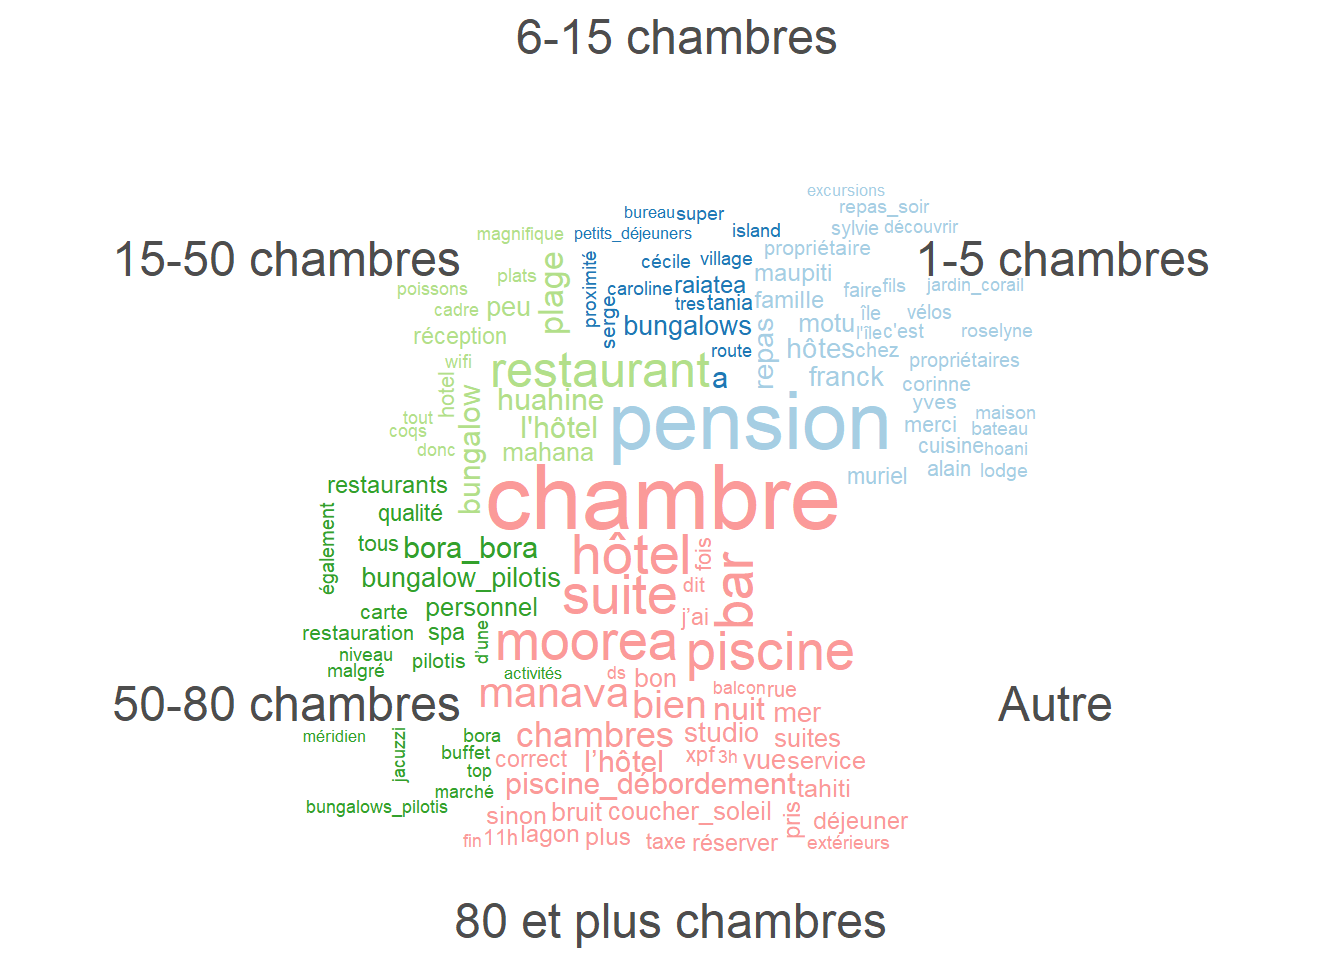
\includegraphics{q07_tokenisation_files/figure-pdf/609-2.pdf}

}

\caption{Mots les plus fréquents du corpus}

\end{figure}%

\section{La question des mots
distinctifs}\label{la-question-des-mots-distinctifs}

Plus que comparer la fréquence des mots on peux souhaiter identifier
ceux qui sont les plus discrimants, les plus distinctifs.

\subsection{Keyness index}\label{keyness-index}

\subsection{Find keywords based on the Textrank
algorithm}\label{find-keywords-based-on-the-textrank-algorithm}

Le Textrank est un algorithme implémenté dans le paquetage R textrank.
Cet algorithme permet de résumer un texte et d'en extraire des
mots-clés. Pour ce faire, il construit un réseau de mots en vérifiant si
les mots se suivent. Sur ce réseau, l'algorithme ``Google Pagerank'' est
appliqué pour extraire les mots pertinents, après quoi les mots
pertinents qui se suivent sont combinés pour obtenir des mots-clés. Dans
l'exemple ci-dessous, nous souhaitons trouver des mots-clés à l'aide de
cet algorithme pour les noms ou les adjectifs qui se suivent. Le
graphique ci-dessous montre que les mots-clés combinent les mots pour
former des expressions à plusieurs mots.

\subsection{Rake}\label{rake}

L'algorithme de base suivant s'appelle RAKE, acronyme de Rapid Automatic
Keyword Extraction (extraction automatique rapide de mots clés). Il
recherche des mots-clés en examinant une séquence contiguë de mots qui
ne contient pas de mots non pertinents. En d'autres termes, il

en calculant un score pour chaque mot faisant partie d'un mot-clé
candidat. parmi les mots des mots-clés candidats, l'algorithme examine
le nombre d'occurrences de chaque mot et le nombre de cooccurrences avec
d'autres mots. Chaque mot obtient un score qui est le rapport entre le
degré du mot (le nombre de fois qu'il cooccurre avec d'autres mots) et
la fréquence du mot. un score RAKE pour le mot-clé candidat complet est
calculé en additionnant les scores de chacun des mots qui définissent le
mot-clé candidat.

\section{Conclusion}\label{conclusion-5}

Dans ce chapitre, nous avons vu comment découper un corpus en unités,
les \emph{tokens}. Nous avons abordé le sujet des n-grammes, et vu
comment composer des \emph{tokens} à partir de concepts multi-mots,
identifiés par des n-grammes adjacents.

On conclue sur l'idée que la distribution des termes d'un texte doit se
comprendre dans deux dimensions : la fréquence des termes parmi tous les
termes, leur fréquence à travers les documents.

\bookmarksetup{startatroot}

\chapter{Annotations syntaxiques}\label{annotations-syntaxiques}

\begin{Shaded}
\begin{Highlighting}[]
\CommentTok{\#les librairies du chapître}
\FunctionTok{library}\NormalTok{(tidyverse)}
\CommentTok{\#accessoires de ggplot}
\FunctionTok{library}\NormalTok{(ggridges)}
\FunctionTok{library}\NormalTok{(ggrepel)}
\FunctionTok{library}\NormalTok{(ggwordcloud)}
\FunctionTok{library}\NormalTok{(igraph)}
\FunctionTok{library}\NormalTok{(ggraph)}

\FunctionTok{theme\_set}\NormalTok{(}\FunctionTok{theme\_minimal}\NormalTok{()) }

\CommentTok{\#NLP}
\FunctionTok{library}\NormalTok{(tokenizers)}
\FunctionTok{library}\NormalTok{(quanteda)}
\FunctionTok{library}\NormalTok{(quanteda.textplots)}
\FunctionTok{library}\NormalTok{(quanteda.textstats )}
\CommentTok{\# glossaire}
\FunctionTok{library}\NormalTok{(glossary)}
\FunctionTok{glossary\_path}\NormalTok{(}\StringTok{"glossary.yml"}\NormalTok{)}
\FunctionTok{glossary\_style}\NormalTok{(}\AttributeTok{color =} \StringTok{"purple"}\NormalTok{, }
               \AttributeTok{text\_decoration =} \StringTok{"underline"}\NormalTok{,}
               \AttributeTok{def\_bg =} \StringTok{"\#333"}\NormalTok{,}
               \AttributeTok{def\_color =} \StringTok{"white"}\NormalTok{)}
\end{Highlighting}
\end{Shaded}

\begin{Shaded}
\begin{Highlighting}[]
\FunctionTok{glossary\_popup}\NormalTok{(}\StringTok{"click"}\NormalTok{)}

\CommentTok{\#tableau}
\FunctionTok{library}\NormalTok{(flextable)}
\FunctionTok{set\_flextable\_defaults}\NormalTok{(}
  \AttributeTok{font.size =} \DecValTok{10}\NormalTok{, }\AttributeTok{theme\_fun =}\NormalTok{ theme\_vanilla,}
  \AttributeTok{padding =} \DecValTok{6}\NormalTok{,}
  \AttributeTok{background.color =} \StringTok{"\#EFEFEF"}\NormalTok{)}

\CommentTok{\#palettes}

\FunctionTok{library}\NormalTok{(wesanderson)}
\CommentTok{\#names(wes\_palettes)}
\NormalTok{col\_1}\OtherTok{\textless{}{-}}\FunctionTok{c}\NormalTok{(}\StringTok{"\#85D4E3"}\NormalTok{)}
\NormalTok{col\_1b}\OtherTok{\textless{}{-}}\FunctionTok{c}\NormalTok{(}\StringTok{"\#F4B5BD"}\NormalTok{)}
\NormalTok{col\_2}\OtherTok{\textless{}{-}}\NormalTok{c }\OtherTok{\textless{}{-}}\FunctionTok{c}\NormalTok{(}\StringTok{"\#85D4E3"}\NormalTok{, }\StringTok{"\#F4B5BD"}\NormalTok{)}
\NormalTok{col\_4}\OtherTok{\textless{}{-}}\FunctionTok{c}\NormalTok{(}\StringTok{"\#85D4E3"}\NormalTok{, }\StringTok{"\#F4B5BD"}\NormalTok{, }\StringTok{"\#9C964A"}\NormalTok{, }\StringTok{"\#CDC08C"}\NormalTok{)}
\end{Highlighting}
\end{Shaded}

\textbf{Objectifs du chapitre :}

\emph{Nous savons désormais manipuler les termes, il est temps de
s'intéresser à leur dimension syntaxique et à examiner comment on peut
les étiqueter pour ajouter de l'information au niveau de chacun des
termes}

L'unité du langage n'est pas le mot, le mot est une unité de lexique.
L'unité du langage se forme dans la glue qui associe les mots, une
chimie pour poursuivre la métaphore, dans la mesure où les règles de la
chimie sont des règles d'association.

Les mots dans la phrases s'associent de manière analogue. Leur glue sont
les règles de syntaxe qui répondent à deux pressions , celle d'une
grammaire naturelle, stochastique surement, et d'une grammaire plus
formelle et conventionnelle que les académies, les groupes de pression
et les communicants.

Cependant, les linguistes ont établi des régularités de catégories
syntaxiques. Notamment les Part of speech, en français les éléments de
langages, des catégories qui s'avère universelles, même si pour décrire
correctement les langues on a besoin de catégories plus spécifiques. Ces
catégories sont les noms communs, les noms propres, les verbes, les
adjectifs, les déterminants, les conjonctions, la ponctuation.

\section{Le processus d'annotation}\label{le-processus-dannotation}

Pour aller au-delà de l'analyse du seul lexique et de l'analyse de la
cooccurence des termes à travers les textes, comme le font les méthodes
de typologie et d'analyse factorielle des correspondance depuis
longtemps, il est nécessaire d'analyser le texte en tenant compte de ses
propriétés syntaxiques. Depuis une dizaine d'années, des outils
puissants, les annotateurs, sont proposés de manière accessible.

Les plus connus sont Spacy, Stanford NLP ou UDpipe avec r .Dans
l'environnement r différentes ressources sont disponibles : Quanteda,
clean\_nlp, Udpipe, \ldots{}

Ils sont disponibles désormais dans de nombreuses langues même si la
richesse et la précision obtenues varient d'une langue à l'autre

Ils s'appuient sur des corpus plus ou moins étendus et spécialisés
d'annotations manuelle : les Treebanks.

Ils réalisent souvent plusieurs tâches dont les principales sont les
suivantes :

\begin{itemize}
\tightlist
\item
  Tokeniser : découper la chaîne de caractère en unité d'analyse( lettre
  syllabe, mot \ldots)
\item
  Lemmatiser : associer à la forme fléchie, le mot racine, celui des
  dictionnaires courants.
\item
  Identifier les parts of speech
\item
  Identifier les dépendances syntaxiques
\item
  Identifier les entités nommées.
\item
  Identifier les co-reférences.
\end{itemize}

Un petit exemple avec le package \texttt{UDpipe}.

\begin{Shaded}
\begin{Highlighting}[]
\FunctionTok{library}\NormalTok{(udpipe)}
\NormalTok{fr }\OtherTok{\textless{}{-}} \FunctionTok{udpipe\_download\_model}\NormalTok{(}\AttributeTok{language =} \StringTok{"french"}\NormalTok{)}
\NormalTok{udmodel\_french }\OtherTok{\textless{}{-}} \FunctionTok{udpipe\_load\_model}\NormalTok{(}\AttributeTok{file =} \StringTok{"french{-}gsd{-}ud{-}2.5{-}191206.udpipe"}\NormalTok{)}
\NormalTok{Citations }\OtherTok{\textless{}{-}} \FunctionTok{read\_csv}\NormalTok{(}\StringTok{"./data/Citations.csv"}\NormalTok{)}

\NormalTok{Flaubert}\OtherTok{\textless{}{-}}\NormalTok{Citations }\SpecialCharTok{\%\textgreater{}\%}
  \FunctionTok{filter}\NormalTok{(doc}\SpecialCharTok{==}\DecValTok{1}\NormalTok{)}

\NormalTok{UD }\OtherTok{\textless{}{-}} \FunctionTok{udpipe\_annotate}\NormalTok{(udmodel\_french, }\AttributeTok{x=}\NormalTok{Flaubert}\SpecialCharTok{$}\NormalTok{text)}
\NormalTok{x }\OtherTok{\textless{}{-}} \FunctionTok{as.data.frame}\NormalTok{(UD)}
\NormalTok{foo}\OtherTok{\textless{}{-}}\NormalTok{x }\SpecialCharTok{\%\textgreater{}\%} 
  \FunctionTok{select}\NormalTok{(doc\_id,paragraph\_id, sentence\_id, token\_id,token,lemma,head\_token\_id, upos,feats)}\SpecialCharTok{\%\textgreater{}\%}\FunctionTok{filter}\NormalTok{(sentence\_id}\SpecialCharTok{==}\DecValTok{1}\NormalTok{)}
\FunctionTok{flextable}\NormalTok{(foo)}
\end{Highlighting}
\end{Shaded}

\global\setlength{\Oldarrayrulewidth}{\arrayrulewidth}

\global\setlength{\Oldtabcolsep}{\tabcolsep}

\setlength{\tabcolsep}{0pt}

\renewcommand*{\arraystretch}{1.5}



\providecommand{\ascline}[3]{\noalign{\global\arrayrulewidth #1}\arrayrulecolor[HTML]{#2}\cline{#3}}

\begin{longtable*}[c]{|p{0.75in}|p{0.75in}|p{0.75in}|p{0.75in}|p{0.75in}|p{0.75in}|p{0.75in}|p{0.75in}|p{0.75in}}



\hhline{>{\arrayrulecolor[HTML]{666666}\global\arrayrulewidth=1.5pt}->{\arrayrulecolor[HTML]{666666}\global\arrayrulewidth=1.5pt}->{\arrayrulecolor[HTML]{666666}\global\arrayrulewidth=1.5pt}->{\arrayrulecolor[HTML]{666666}\global\arrayrulewidth=1.5pt}->{\arrayrulecolor[HTML]{666666}\global\arrayrulewidth=1.5pt}->{\arrayrulecolor[HTML]{666666}\global\arrayrulewidth=1.5pt}->{\arrayrulecolor[HTML]{666666}\global\arrayrulewidth=1.5pt}->{\arrayrulecolor[HTML]{666666}\global\arrayrulewidth=1.5pt}->{\arrayrulecolor[HTML]{666666}\global\arrayrulewidth=1.5pt}-}

\multicolumn{1}{>{\cellcolor[HTML]{EFEFEF}\raggedright}m{\dimexpr 0.75in+0\tabcolsep}}{\textcolor[HTML]{000000}{\fontsize{10}{10}\selectfont{\textbf{doc\_id}}}} & \multicolumn{1}{>{\cellcolor[HTML]{EFEFEF}\raggedleft}m{\dimexpr 0.75in+0\tabcolsep}}{\textcolor[HTML]{000000}{\fontsize{10}{10}\selectfont{\textbf{paragraph\_id}}}} & \multicolumn{1}{>{\cellcolor[HTML]{EFEFEF}\raggedleft}m{\dimexpr 0.75in+0\tabcolsep}}{\textcolor[HTML]{000000}{\fontsize{10}{10}\selectfont{\textbf{sentence\_id}}}} & \multicolumn{1}{>{\cellcolor[HTML]{EFEFEF}\raggedright}m{\dimexpr 0.75in+0\tabcolsep}}{\textcolor[HTML]{000000}{\fontsize{10}{10}\selectfont{\textbf{token\_id}}}} & \multicolumn{1}{>{\cellcolor[HTML]{EFEFEF}\raggedright}m{\dimexpr 0.75in+0\tabcolsep}}{\textcolor[HTML]{000000}{\fontsize{10}{10}\selectfont{\textbf{token}}}} & \multicolumn{1}{>{\cellcolor[HTML]{EFEFEF}\raggedright}m{\dimexpr 0.75in+0\tabcolsep}}{\textcolor[HTML]{000000}{\fontsize{10}{10}\selectfont{\textbf{lemma}}}} & \multicolumn{1}{>{\cellcolor[HTML]{EFEFEF}\raggedright}m{\dimexpr 0.75in+0\tabcolsep}}{\textcolor[HTML]{000000}{\fontsize{10}{10}\selectfont{\textbf{head\_token\_id}}}} & \multicolumn{1}{>{\cellcolor[HTML]{EFEFEF}\raggedright}m{\dimexpr 0.75in+0\tabcolsep}}{\textcolor[HTML]{000000}{\fontsize{10}{10}\selectfont{\textbf{upos}}}} & \multicolumn{1}{>{\cellcolor[HTML]{EFEFEF}\raggedright}m{\dimexpr 0.75in+0\tabcolsep}}{\textcolor[HTML]{000000}{\fontsize{10}{10}\selectfont{\textbf{feats}}}} \\

\noalign{\global\arrayrulewidth 0pt}\arrayrulecolor[HTML]{000000}

\hhline{>{\arrayrulecolor[HTML]{666666}\global\arrayrulewidth=1.5pt}->{\arrayrulecolor[HTML]{666666}\global\arrayrulewidth=1.5pt}->{\arrayrulecolor[HTML]{666666}\global\arrayrulewidth=1.5pt}->{\arrayrulecolor[HTML]{666666}\global\arrayrulewidth=1.5pt}->{\arrayrulecolor[HTML]{666666}\global\arrayrulewidth=1.5pt}->{\arrayrulecolor[HTML]{666666}\global\arrayrulewidth=1.5pt}->{\arrayrulecolor[HTML]{666666}\global\arrayrulewidth=1.5pt}->{\arrayrulecolor[HTML]{666666}\global\arrayrulewidth=1.5pt}->{\arrayrulecolor[HTML]{666666}\global\arrayrulewidth=1.5pt}-}\endfirsthead 

\hhline{>{\arrayrulecolor[HTML]{666666}\global\arrayrulewidth=1.5pt}->{\arrayrulecolor[HTML]{666666}\global\arrayrulewidth=1.5pt}->{\arrayrulecolor[HTML]{666666}\global\arrayrulewidth=1.5pt}->{\arrayrulecolor[HTML]{666666}\global\arrayrulewidth=1.5pt}->{\arrayrulecolor[HTML]{666666}\global\arrayrulewidth=1.5pt}->{\arrayrulecolor[HTML]{666666}\global\arrayrulewidth=1.5pt}->{\arrayrulecolor[HTML]{666666}\global\arrayrulewidth=1.5pt}->{\arrayrulecolor[HTML]{666666}\global\arrayrulewidth=1.5pt}->{\arrayrulecolor[HTML]{666666}\global\arrayrulewidth=1.5pt}-}

\multicolumn{1}{>{\cellcolor[HTML]{EFEFEF}\raggedright}m{\dimexpr 0.75in+0\tabcolsep}}{\textcolor[HTML]{000000}{\fontsize{10}{10}\selectfont{\textbf{doc\_id}}}} & \multicolumn{1}{>{\cellcolor[HTML]{EFEFEF}\raggedleft}m{\dimexpr 0.75in+0\tabcolsep}}{\textcolor[HTML]{000000}{\fontsize{10}{10}\selectfont{\textbf{paragraph\_id}}}} & \multicolumn{1}{>{\cellcolor[HTML]{EFEFEF}\raggedleft}m{\dimexpr 0.75in+0\tabcolsep}}{\textcolor[HTML]{000000}{\fontsize{10}{10}\selectfont{\textbf{sentence\_id}}}} & \multicolumn{1}{>{\cellcolor[HTML]{EFEFEF}\raggedright}m{\dimexpr 0.75in+0\tabcolsep}}{\textcolor[HTML]{000000}{\fontsize{10}{10}\selectfont{\textbf{token\_id}}}} & \multicolumn{1}{>{\cellcolor[HTML]{EFEFEF}\raggedright}m{\dimexpr 0.75in+0\tabcolsep}}{\textcolor[HTML]{000000}{\fontsize{10}{10}\selectfont{\textbf{token}}}} & \multicolumn{1}{>{\cellcolor[HTML]{EFEFEF}\raggedright}m{\dimexpr 0.75in+0\tabcolsep}}{\textcolor[HTML]{000000}{\fontsize{10}{10}\selectfont{\textbf{lemma}}}} & \multicolumn{1}{>{\cellcolor[HTML]{EFEFEF}\raggedright}m{\dimexpr 0.75in+0\tabcolsep}}{\textcolor[HTML]{000000}{\fontsize{10}{10}\selectfont{\textbf{head\_token\_id}}}} & \multicolumn{1}{>{\cellcolor[HTML]{EFEFEF}\raggedright}m{\dimexpr 0.75in+0\tabcolsep}}{\textcolor[HTML]{000000}{\fontsize{10}{10}\selectfont{\textbf{upos}}}} & \multicolumn{1}{>{\cellcolor[HTML]{EFEFEF}\raggedright}m{\dimexpr 0.75in+0\tabcolsep}}{\textcolor[HTML]{000000}{\fontsize{10}{10}\selectfont{\textbf{feats}}}} \\

\noalign{\global\arrayrulewidth 0pt}\arrayrulecolor[HTML]{000000}

\hhline{>{\arrayrulecolor[HTML]{666666}\global\arrayrulewidth=1.5pt}->{\arrayrulecolor[HTML]{666666}\global\arrayrulewidth=1.5pt}->{\arrayrulecolor[HTML]{666666}\global\arrayrulewidth=1.5pt}->{\arrayrulecolor[HTML]{666666}\global\arrayrulewidth=1.5pt}->{\arrayrulecolor[HTML]{666666}\global\arrayrulewidth=1.5pt}->{\arrayrulecolor[HTML]{666666}\global\arrayrulewidth=1.5pt}->{\arrayrulecolor[HTML]{666666}\global\arrayrulewidth=1.5pt}->{\arrayrulecolor[HTML]{666666}\global\arrayrulewidth=1.5pt}->{\arrayrulecolor[HTML]{666666}\global\arrayrulewidth=1.5pt}-}\endhead



\multicolumn{1}{>{\cellcolor[HTML]{EFEFEF}\raggedright}m{\dimexpr 0.75in+0\tabcolsep}}{\textcolor[HTML]{000000}{\fontsize{10}{10}\selectfont{doc1}}} & \multicolumn{1}{>{\cellcolor[HTML]{EFEFEF}\raggedleft}m{\dimexpr 0.75in+0\tabcolsep}}{\textcolor[HTML]{000000}{\fontsize{10}{10}\selectfont{1}}} & \multicolumn{1}{>{\cellcolor[HTML]{EFEFEF}\raggedleft}m{\dimexpr 0.75in+0\tabcolsep}}{\textcolor[HTML]{000000}{\fontsize{10}{10}\selectfont{1}}} & \multicolumn{1}{>{\cellcolor[HTML]{EFEFEF}\raggedright}m{\dimexpr 0.75in+0\tabcolsep}}{\textcolor[HTML]{000000}{\fontsize{10}{10}\selectfont{1}}} & \multicolumn{1}{>{\cellcolor[HTML]{EFEFEF}\raggedright}m{\dimexpr 0.75in+0\tabcolsep}}{\textcolor[HTML]{000000}{\fontsize{10}{10}\selectfont{Le}}} & \multicolumn{1}{>{\cellcolor[HTML]{EFEFEF}\raggedright}m{\dimexpr 0.75in+0\tabcolsep}}{\textcolor[HTML]{000000}{\fontsize{10}{10}\selectfont{le}}} & \multicolumn{1}{>{\cellcolor[HTML]{EFEFEF}\raggedright}m{\dimexpr 0.75in+0\tabcolsep}}{\textcolor[HTML]{000000}{\fontsize{10}{10}\selectfont{2}}} & \multicolumn{1}{>{\cellcolor[HTML]{EFEFEF}\raggedright}m{\dimexpr 0.75in+0\tabcolsep}}{\textcolor[HTML]{000000}{\fontsize{10}{10}\selectfont{DET}}} & \multicolumn{1}{>{\cellcolor[HTML]{EFEFEF}\raggedright}m{\dimexpr 0.75in+0\tabcolsep}}{\textcolor[HTML]{000000}{\fontsize{10}{10}\selectfont{Definite=Def|Gender=Masc|Number=Sing|PronType=Art}}} \\

\noalign{\global\arrayrulewidth 0pt}\arrayrulecolor[HTML]{000000}

\hhline{>{\arrayrulecolor[HTML]{666666}\global\arrayrulewidth=0.75pt}->{\arrayrulecolor[HTML]{666666}\global\arrayrulewidth=0.75pt}->{\arrayrulecolor[HTML]{666666}\global\arrayrulewidth=0.75pt}->{\arrayrulecolor[HTML]{666666}\global\arrayrulewidth=0.75pt}->{\arrayrulecolor[HTML]{666666}\global\arrayrulewidth=0.75pt}->{\arrayrulecolor[HTML]{666666}\global\arrayrulewidth=0.75pt}->{\arrayrulecolor[HTML]{666666}\global\arrayrulewidth=0.75pt}->{\arrayrulecolor[HTML]{666666}\global\arrayrulewidth=0.75pt}->{\arrayrulecolor[HTML]{666666}\global\arrayrulewidth=0.75pt}-}



\multicolumn{1}{>{\cellcolor[HTML]{EFEFEF}\raggedright}m{\dimexpr 0.75in+0\tabcolsep}}{\textcolor[HTML]{000000}{\fontsize{10}{10}\selectfont{doc1}}} & \multicolumn{1}{>{\cellcolor[HTML]{EFEFEF}\raggedleft}m{\dimexpr 0.75in+0\tabcolsep}}{\textcolor[HTML]{000000}{\fontsize{10}{10}\selectfont{1}}} & \multicolumn{1}{>{\cellcolor[HTML]{EFEFEF}\raggedleft}m{\dimexpr 0.75in+0\tabcolsep}}{\textcolor[HTML]{000000}{\fontsize{10}{10}\selectfont{1}}} & \multicolumn{1}{>{\cellcolor[HTML]{EFEFEF}\raggedright}m{\dimexpr 0.75in+0\tabcolsep}}{\textcolor[HTML]{000000}{\fontsize{10}{10}\selectfont{2}}} & \multicolumn{1}{>{\cellcolor[HTML]{EFEFEF}\raggedright}m{\dimexpr 0.75in+0\tabcolsep}}{\textcolor[HTML]{000000}{\fontsize{10}{10}\selectfont{lendemain}}} & \multicolumn{1}{>{\cellcolor[HTML]{EFEFEF}\raggedright}m{\dimexpr 0.75in+0\tabcolsep}}{\textcolor[HTML]{000000}{\fontsize{10}{10}\selectfont{lendemain}}} & \multicolumn{1}{>{\cellcolor[HTML]{EFEFEF}\raggedright}m{\dimexpr 0.75in+0\tabcolsep}}{\textcolor[HTML]{000000}{\fontsize{10}{10}\selectfont{9}}} & \multicolumn{1}{>{\cellcolor[HTML]{EFEFEF}\raggedright}m{\dimexpr 0.75in+0\tabcolsep}}{\textcolor[HTML]{000000}{\fontsize{10}{10}\selectfont{NOUN}}} & \multicolumn{1}{>{\cellcolor[HTML]{EFEFEF}\raggedright}m{\dimexpr 0.75in+0\tabcolsep}}{\textcolor[HTML]{000000}{\fontsize{10}{10}\selectfont{Gender=Masc|Number=Sing}}} \\

\noalign{\global\arrayrulewidth 0pt}\arrayrulecolor[HTML]{000000}

\hhline{>{\arrayrulecolor[HTML]{666666}\global\arrayrulewidth=0.75pt}->{\arrayrulecolor[HTML]{666666}\global\arrayrulewidth=0.75pt}->{\arrayrulecolor[HTML]{666666}\global\arrayrulewidth=0.75pt}->{\arrayrulecolor[HTML]{666666}\global\arrayrulewidth=0.75pt}->{\arrayrulecolor[HTML]{666666}\global\arrayrulewidth=0.75pt}->{\arrayrulecolor[HTML]{666666}\global\arrayrulewidth=0.75pt}->{\arrayrulecolor[HTML]{666666}\global\arrayrulewidth=0.75pt}->{\arrayrulecolor[HTML]{666666}\global\arrayrulewidth=0.75pt}->{\arrayrulecolor[HTML]{666666}\global\arrayrulewidth=0.75pt}-}



\multicolumn{1}{>{\cellcolor[HTML]{EFEFEF}\raggedright}m{\dimexpr 0.75in+0\tabcolsep}}{\textcolor[HTML]{000000}{\fontsize{10}{10}\selectfont{doc1}}} & \multicolumn{1}{>{\cellcolor[HTML]{EFEFEF}\raggedleft}m{\dimexpr 0.75in+0\tabcolsep}}{\textcolor[HTML]{000000}{\fontsize{10}{10}\selectfont{1}}} & \multicolumn{1}{>{\cellcolor[HTML]{EFEFEF}\raggedleft}m{\dimexpr 0.75in+0\tabcolsep}}{\textcolor[HTML]{000000}{\fontsize{10}{10}\selectfont{1}}} & \multicolumn{1}{>{\cellcolor[HTML]{EFEFEF}\raggedright}m{\dimexpr 0.75in+0\tabcolsep}}{\textcolor[HTML]{000000}{\fontsize{10}{10}\selectfont{3}}} & \multicolumn{1}{>{\cellcolor[HTML]{EFEFEF}\raggedright}m{\dimexpr 0.75in+0\tabcolsep}}{\textcolor[HTML]{000000}{\fontsize{10}{10}\selectfont{fut}}} & \multicolumn{1}{>{\cellcolor[HTML]{EFEFEF}\raggedright}m{\dimexpr 0.75in+0\tabcolsep}}{\textcolor[HTML]{000000}{\fontsize{10}{10}\selectfont{être}}} & \multicolumn{1}{>{\cellcolor[HTML]{EFEFEF}\raggedright}m{\dimexpr 0.75in+0\tabcolsep}}{\textcolor[HTML]{000000}{\fontsize{10}{10}\selectfont{9}}} & \multicolumn{1}{>{\cellcolor[HTML]{EFEFEF}\raggedright}m{\dimexpr 0.75in+0\tabcolsep}}{\textcolor[HTML]{000000}{\fontsize{10}{10}\selectfont{AUX}}} & \multicolumn{1}{>{\cellcolor[HTML]{EFEFEF}\raggedright}m{\dimexpr 0.75in+0\tabcolsep}}{\textcolor[HTML]{000000}{\fontsize{10}{10}\selectfont{Mood=Ind|Number=Sing|Person=3|Tense=Past|VerbForm=Fin}}} \\

\noalign{\global\arrayrulewidth 0pt}\arrayrulecolor[HTML]{000000}

\hhline{>{\arrayrulecolor[HTML]{666666}\global\arrayrulewidth=0.75pt}->{\arrayrulecolor[HTML]{666666}\global\arrayrulewidth=0.75pt}->{\arrayrulecolor[HTML]{666666}\global\arrayrulewidth=0.75pt}->{\arrayrulecolor[HTML]{666666}\global\arrayrulewidth=0.75pt}->{\arrayrulecolor[HTML]{666666}\global\arrayrulewidth=0.75pt}->{\arrayrulecolor[HTML]{666666}\global\arrayrulewidth=0.75pt}->{\arrayrulecolor[HTML]{666666}\global\arrayrulewidth=0.75pt}->{\arrayrulecolor[HTML]{666666}\global\arrayrulewidth=0.75pt}->{\arrayrulecolor[HTML]{666666}\global\arrayrulewidth=0.75pt}-}



\multicolumn{1}{>{\cellcolor[HTML]{EFEFEF}\raggedright}m{\dimexpr 0.75in+0\tabcolsep}}{\textcolor[HTML]{000000}{\fontsize{10}{10}\selectfont{doc1}}} & \multicolumn{1}{>{\cellcolor[HTML]{EFEFEF}\raggedleft}m{\dimexpr 0.75in+0\tabcolsep}}{\textcolor[HTML]{000000}{\fontsize{10}{10}\selectfont{1}}} & \multicolumn{1}{>{\cellcolor[HTML]{EFEFEF}\raggedleft}m{\dimexpr 0.75in+0\tabcolsep}}{\textcolor[HTML]{000000}{\fontsize{10}{10}\selectfont{1}}} & \multicolumn{1}{>{\cellcolor[HTML]{EFEFEF}\raggedright}m{\dimexpr 0.75in+0\tabcolsep}}{\textcolor[HTML]{000000}{\fontsize{10}{10}\selectfont{4}}} & \multicolumn{1}{>{\cellcolor[HTML]{EFEFEF}\raggedright}m{\dimexpr 0.75in+0\tabcolsep}}{\textcolor[HTML]{000000}{\fontsize{10}{10}\selectfont{,}}} & \multicolumn{1}{>{\cellcolor[HTML]{EFEFEF}\raggedright}m{\dimexpr 0.75in+0\tabcolsep}}{\textcolor[HTML]{000000}{\fontsize{10}{10}\selectfont{,}}} & \multicolumn{1}{>{\cellcolor[HTML]{EFEFEF}\raggedright}m{\dimexpr 0.75in+0\tabcolsep}}{\textcolor[HTML]{000000}{\fontsize{10}{10}\selectfont{6}}} & \multicolumn{1}{>{\cellcolor[HTML]{EFEFEF}\raggedright}m{\dimexpr 0.75in+0\tabcolsep}}{\textcolor[HTML]{000000}{\fontsize{10}{10}\selectfont{PUNCT}}} & \multicolumn{1}{>{\cellcolor[HTML]{EFEFEF}\raggedright}m{\dimexpr 0.75in+0\tabcolsep}}{\textcolor[HTML]{000000}{\fontsize{10}{10}\selectfont{}}} \\

\noalign{\global\arrayrulewidth 0pt}\arrayrulecolor[HTML]{000000}

\hhline{>{\arrayrulecolor[HTML]{666666}\global\arrayrulewidth=0.75pt}->{\arrayrulecolor[HTML]{666666}\global\arrayrulewidth=0.75pt}->{\arrayrulecolor[HTML]{666666}\global\arrayrulewidth=0.75pt}->{\arrayrulecolor[HTML]{666666}\global\arrayrulewidth=0.75pt}->{\arrayrulecolor[HTML]{666666}\global\arrayrulewidth=0.75pt}->{\arrayrulecolor[HTML]{666666}\global\arrayrulewidth=0.75pt}->{\arrayrulecolor[HTML]{666666}\global\arrayrulewidth=0.75pt}->{\arrayrulecolor[HTML]{666666}\global\arrayrulewidth=0.75pt}->{\arrayrulecolor[HTML]{666666}\global\arrayrulewidth=0.75pt}-}



\multicolumn{1}{>{\cellcolor[HTML]{EFEFEF}\raggedright}m{\dimexpr 0.75in+0\tabcolsep}}{\textcolor[HTML]{000000}{\fontsize{10}{10}\selectfont{doc1}}} & \multicolumn{1}{>{\cellcolor[HTML]{EFEFEF}\raggedleft}m{\dimexpr 0.75in+0\tabcolsep}}{\textcolor[HTML]{000000}{\fontsize{10}{10}\selectfont{1}}} & \multicolumn{1}{>{\cellcolor[HTML]{EFEFEF}\raggedleft}m{\dimexpr 0.75in+0\tabcolsep}}{\textcolor[HTML]{000000}{\fontsize{10}{10}\selectfont{1}}} & \multicolumn{1}{>{\cellcolor[HTML]{EFEFEF}\raggedright}m{\dimexpr 0.75in+0\tabcolsep}}{\textcolor[HTML]{000000}{\fontsize{10}{10}\selectfont{5}}} & \multicolumn{1}{>{\cellcolor[HTML]{EFEFEF}\raggedright}m{\dimexpr 0.75in+0\tabcolsep}}{\textcolor[HTML]{000000}{\fontsize{10}{10}\selectfont{pour}}} & \multicolumn{1}{>{\cellcolor[HTML]{EFEFEF}\raggedright}m{\dimexpr 0.75in+0\tabcolsep}}{\textcolor[HTML]{000000}{\fontsize{10}{10}\selectfont{pour}}} & \multicolumn{1}{>{\cellcolor[HTML]{EFEFEF}\raggedright}m{\dimexpr 0.75in+0\tabcolsep}}{\textcolor[HTML]{000000}{\fontsize{10}{10}\selectfont{6}}} & \multicolumn{1}{>{\cellcolor[HTML]{EFEFEF}\raggedright}m{\dimexpr 0.75in+0\tabcolsep}}{\textcolor[HTML]{000000}{\fontsize{10}{10}\selectfont{ADP}}} & \multicolumn{1}{>{\cellcolor[HTML]{EFEFEF}\raggedright}m{\dimexpr 0.75in+0\tabcolsep}}{\textcolor[HTML]{000000}{\fontsize{10}{10}\selectfont{}}} \\

\noalign{\global\arrayrulewidth 0pt}\arrayrulecolor[HTML]{000000}

\hhline{>{\arrayrulecolor[HTML]{666666}\global\arrayrulewidth=0.75pt}->{\arrayrulecolor[HTML]{666666}\global\arrayrulewidth=0.75pt}->{\arrayrulecolor[HTML]{666666}\global\arrayrulewidth=0.75pt}->{\arrayrulecolor[HTML]{666666}\global\arrayrulewidth=0.75pt}->{\arrayrulecolor[HTML]{666666}\global\arrayrulewidth=0.75pt}->{\arrayrulecolor[HTML]{666666}\global\arrayrulewidth=0.75pt}->{\arrayrulecolor[HTML]{666666}\global\arrayrulewidth=0.75pt}->{\arrayrulecolor[HTML]{666666}\global\arrayrulewidth=0.75pt}->{\arrayrulecolor[HTML]{666666}\global\arrayrulewidth=0.75pt}-}



\multicolumn{1}{>{\cellcolor[HTML]{EFEFEF}\raggedright}m{\dimexpr 0.75in+0\tabcolsep}}{\textcolor[HTML]{000000}{\fontsize{10}{10}\selectfont{doc1}}} & \multicolumn{1}{>{\cellcolor[HTML]{EFEFEF}\raggedleft}m{\dimexpr 0.75in+0\tabcolsep}}{\textcolor[HTML]{000000}{\fontsize{10}{10}\selectfont{1}}} & \multicolumn{1}{>{\cellcolor[HTML]{EFEFEF}\raggedleft}m{\dimexpr 0.75in+0\tabcolsep}}{\textcolor[HTML]{000000}{\fontsize{10}{10}\selectfont{1}}} & \multicolumn{1}{>{\cellcolor[HTML]{EFEFEF}\raggedright}m{\dimexpr 0.75in+0\tabcolsep}}{\textcolor[HTML]{000000}{\fontsize{10}{10}\selectfont{6}}} & \multicolumn{1}{>{\cellcolor[HTML]{EFEFEF}\raggedright}m{\dimexpr 0.75in+0\tabcolsep}}{\textcolor[HTML]{000000}{\fontsize{10}{10}\selectfont{Emma}}} & \multicolumn{1}{>{\cellcolor[HTML]{EFEFEF}\raggedright}m{\dimexpr 0.75in+0\tabcolsep}}{\textcolor[HTML]{000000}{\fontsize{10}{10}\selectfont{Emma}}} & \multicolumn{1}{>{\cellcolor[HTML]{EFEFEF}\raggedright}m{\dimexpr 0.75in+0\tabcolsep}}{\textcolor[HTML]{000000}{\fontsize{10}{10}\selectfont{9}}} & \multicolumn{1}{>{\cellcolor[HTML]{EFEFEF}\raggedright}m{\dimexpr 0.75in+0\tabcolsep}}{\textcolor[HTML]{000000}{\fontsize{10}{10}\selectfont{PROPN}}} & \multicolumn{1}{>{\cellcolor[HTML]{EFEFEF}\raggedright}m{\dimexpr 0.75in+0\tabcolsep}}{\textcolor[HTML]{000000}{\fontsize{10}{10}\selectfont{}}} \\

\noalign{\global\arrayrulewidth 0pt}\arrayrulecolor[HTML]{000000}

\hhline{>{\arrayrulecolor[HTML]{666666}\global\arrayrulewidth=0.75pt}->{\arrayrulecolor[HTML]{666666}\global\arrayrulewidth=0.75pt}->{\arrayrulecolor[HTML]{666666}\global\arrayrulewidth=0.75pt}->{\arrayrulecolor[HTML]{666666}\global\arrayrulewidth=0.75pt}->{\arrayrulecolor[HTML]{666666}\global\arrayrulewidth=0.75pt}->{\arrayrulecolor[HTML]{666666}\global\arrayrulewidth=0.75pt}->{\arrayrulecolor[HTML]{666666}\global\arrayrulewidth=0.75pt}->{\arrayrulecolor[HTML]{666666}\global\arrayrulewidth=0.75pt}->{\arrayrulecolor[HTML]{666666}\global\arrayrulewidth=0.75pt}-}



\multicolumn{1}{>{\cellcolor[HTML]{EFEFEF}\raggedright}m{\dimexpr 0.75in+0\tabcolsep}}{\textcolor[HTML]{000000}{\fontsize{10}{10}\selectfont{doc1}}} & \multicolumn{1}{>{\cellcolor[HTML]{EFEFEF}\raggedleft}m{\dimexpr 0.75in+0\tabcolsep}}{\textcolor[HTML]{000000}{\fontsize{10}{10}\selectfont{1}}} & \multicolumn{1}{>{\cellcolor[HTML]{EFEFEF}\raggedleft}m{\dimexpr 0.75in+0\tabcolsep}}{\textcolor[HTML]{000000}{\fontsize{10}{10}\selectfont{1}}} & \multicolumn{1}{>{\cellcolor[HTML]{EFEFEF}\raggedright}m{\dimexpr 0.75in+0\tabcolsep}}{\textcolor[HTML]{000000}{\fontsize{10}{10}\selectfont{7}}} & \multicolumn{1}{>{\cellcolor[HTML]{EFEFEF}\raggedright}m{\dimexpr 0.75in+0\tabcolsep}}{\textcolor[HTML]{000000}{\fontsize{10}{10}\selectfont{,}}} & \multicolumn{1}{>{\cellcolor[HTML]{EFEFEF}\raggedright}m{\dimexpr 0.75in+0\tabcolsep}}{\textcolor[HTML]{000000}{\fontsize{10}{10}\selectfont{,}}} & \multicolumn{1}{>{\cellcolor[HTML]{EFEFEF}\raggedright}m{\dimexpr 0.75in+0\tabcolsep}}{\textcolor[HTML]{000000}{\fontsize{10}{10}\selectfont{6}}} & \multicolumn{1}{>{\cellcolor[HTML]{EFEFEF}\raggedright}m{\dimexpr 0.75in+0\tabcolsep}}{\textcolor[HTML]{000000}{\fontsize{10}{10}\selectfont{PUNCT}}} & \multicolumn{1}{>{\cellcolor[HTML]{EFEFEF}\raggedright}m{\dimexpr 0.75in+0\tabcolsep}}{\textcolor[HTML]{000000}{\fontsize{10}{10}\selectfont{}}} \\

\noalign{\global\arrayrulewidth 0pt}\arrayrulecolor[HTML]{000000}

\hhline{>{\arrayrulecolor[HTML]{666666}\global\arrayrulewidth=0.75pt}->{\arrayrulecolor[HTML]{666666}\global\arrayrulewidth=0.75pt}->{\arrayrulecolor[HTML]{666666}\global\arrayrulewidth=0.75pt}->{\arrayrulecolor[HTML]{666666}\global\arrayrulewidth=0.75pt}->{\arrayrulecolor[HTML]{666666}\global\arrayrulewidth=0.75pt}->{\arrayrulecolor[HTML]{666666}\global\arrayrulewidth=0.75pt}->{\arrayrulecolor[HTML]{666666}\global\arrayrulewidth=0.75pt}->{\arrayrulecolor[HTML]{666666}\global\arrayrulewidth=0.75pt}->{\arrayrulecolor[HTML]{666666}\global\arrayrulewidth=0.75pt}-}



\multicolumn{1}{>{\cellcolor[HTML]{EFEFEF}\raggedright}m{\dimexpr 0.75in+0\tabcolsep}}{\textcolor[HTML]{000000}{\fontsize{10}{10}\selectfont{doc1}}} & \multicolumn{1}{>{\cellcolor[HTML]{EFEFEF}\raggedleft}m{\dimexpr 0.75in+0\tabcolsep}}{\textcolor[HTML]{000000}{\fontsize{10}{10}\selectfont{1}}} & \multicolumn{1}{>{\cellcolor[HTML]{EFEFEF}\raggedleft}m{\dimexpr 0.75in+0\tabcolsep}}{\textcolor[HTML]{000000}{\fontsize{10}{10}\selectfont{1}}} & \multicolumn{1}{>{\cellcolor[HTML]{EFEFEF}\raggedright}m{\dimexpr 0.75in+0\tabcolsep}}{\textcolor[HTML]{000000}{\fontsize{10}{10}\selectfont{8}}} & \multicolumn{1}{>{\cellcolor[HTML]{EFEFEF}\raggedright}m{\dimexpr 0.75in+0\tabcolsep}}{\textcolor[HTML]{000000}{\fontsize{10}{10}\selectfont{une}}} & \multicolumn{1}{>{\cellcolor[HTML]{EFEFEF}\raggedright}m{\dimexpr 0.75in+0\tabcolsep}}{\textcolor[HTML]{000000}{\fontsize{10}{10}\selectfont{un}}} & \multicolumn{1}{>{\cellcolor[HTML]{EFEFEF}\raggedright}m{\dimexpr 0.75in+0\tabcolsep}}{\textcolor[HTML]{000000}{\fontsize{10}{10}\selectfont{9}}} & \multicolumn{1}{>{\cellcolor[HTML]{EFEFEF}\raggedright}m{\dimexpr 0.75in+0\tabcolsep}}{\textcolor[HTML]{000000}{\fontsize{10}{10}\selectfont{DET}}} & \multicolumn{1}{>{\cellcolor[HTML]{EFEFEF}\raggedright}m{\dimexpr 0.75in+0\tabcolsep}}{\textcolor[HTML]{000000}{\fontsize{10}{10}\selectfont{Definite=Ind|Gender=Fem|Number=Sing|PronType=Art}}} \\

\noalign{\global\arrayrulewidth 0pt}\arrayrulecolor[HTML]{000000}

\hhline{>{\arrayrulecolor[HTML]{666666}\global\arrayrulewidth=0.75pt}->{\arrayrulecolor[HTML]{666666}\global\arrayrulewidth=0.75pt}->{\arrayrulecolor[HTML]{666666}\global\arrayrulewidth=0.75pt}->{\arrayrulecolor[HTML]{666666}\global\arrayrulewidth=0.75pt}->{\arrayrulecolor[HTML]{666666}\global\arrayrulewidth=0.75pt}->{\arrayrulecolor[HTML]{666666}\global\arrayrulewidth=0.75pt}->{\arrayrulecolor[HTML]{666666}\global\arrayrulewidth=0.75pt}->{\arrayrulecolor[HTML]{666666}\global\arrayrulewidth=0.75pt}->{\arrayrulecolor[HTML]{666666}\global\arrayrulewidth=0.75pt}-}



\multicolumn{1}{>{\cellcolor[HTML]{EFEFEF}\raggedright}m{\dimexpr 0.75in+0\tabcolsep}}{\textcolor[HTML]{000000}{\fontsize{10}{10}\selectfont{doc1}}} & \multicolumn{1}{>{\cellcolor[HTML]{EFEFEF}\raggedleft}m{\dimexpr 0.75in+0\tabcolsep}}{\textcolor[HTML]{000000}{\fontsize{10}{10}\selectfont{1}}} & \multicolumn{1}{>{\cellcolor[HTML]{EFEFEF}\raggedleft}m{\dimexpr 0.75in+0\tabcolsep}}{\textcolor[HTML]{000000}{\fontsize{10}{10}\selectfont{1}}} & \multicolumn{1}{>{\cellcolor[HTML]{EFEFEF}\raggedright}m{\dimexpr 0.75in+0\tabcolsep}}{\textcolor[HTML]{000000}{\fontsize{10}{10}\selectfont{9}}} & \multicolumn{1}{>{\cellcolor[HTML]{EFEFEF}\raggedright}m{\dimexpr 0.75in+0\tabcolsep}}{\textcolor[HTML]{000000}{\fontsize{10}{10}\selectfont{journée}}} & \multicolumn{1}{>{\cellcolor[HTML]{EFEFEF}\raggedright}m{\dimexpr 0.75in+0\tabcolsep}}{\textcolor[HTML]{000000}{\fontsize{10}{10}\selectfont{journée}}} & \multicolumn{1}{>{\cellcolor[HTML]{EFEFEF}\raggedright}m{\dimexpr 0.75in+0\tabcolsep}}{\textcolor[HTML]{000000}{\fontsize{10}{10}\selectfont{0}}} & \multicolumn{1}{>{\cellcolor[HTML]{EFEFEF}\raggedright}m{\dimexpr 0.75in+0\tabcolsep}}{\textcolor[HTML]{000000}{\fontsize{10}{10}\selectfont{NOUN}}} & \multicolumn{1}{>{\cellcolor[HTML]{EFEFEF}\raggedright}m{\dimexpr 0.75in+0\tabcolsep}}{\textcolor[HTML]{000000}{\fontsize{10}{10}\selectfont{Gender=Fem|Number=Sing}}} \\

\noalign{\global\arrayrulewidth 0pt}\arrayrulecolor[HTML]{000000}

\hhline{>{\arrayrulecolor[HTML]{666666}\global\arrayrulewidth=0.75pt}->{\arrayrulecolor[HTML]{666666}\global\arrayrulewidth=0.75pt}->{\arrayrulecolor[HTML]{666666}\global\arrayrulewidth=0.75pt}->{\arrayrulecolor[HTML]{666666}\global\arrayrulewidth=0.75pt}->{\arrayrulecolor[HTML]{666666}\global\arrayrulewidth=0.75pt}->{\arrayrulecolor[HTML]{666666}\global\arrayrulewidth=0.75pt}->{\arrayrulecolor[HTML]{666666}\global\arrayrulewidth=0.75pt}->{\arrayrulecolor[HTML]{666666}\global\arrayrulewidth=0.75pt}->{\arrayrulecolor[HTML]{666666}\global\arrayrulewidth=0.75pt}-}



\multicolumn{1}{>{\cellcolor[HTML]{EFEFEF}\raggedright}m{\dimexpr 0.75in+0\tabcolsep}}{\textcolor[HTML]{000000}{\fontsize{10}{10}\selectfont{doc1}}} & \multicolumn{1}{>{\cellcolor[HTML]{EFEFEF}\raggedleft}m{\dimexpr 0.75in+0\tabcolsep}}{\textcolor[HTML]{000000}{\fontsize{10}{10}\selectfont{1}}} & \multicolumn{1}{>{\cellcolor[HTML]{EFEFEF}\raggedleft}m{\dimexpr 0.75in+0\tabcolsep}}{\textcolor[HTML]{000000}{\fontsize{10}{10}\selectfont{1}}} & \multicolumn{1}{>{\cellcolor[HTML]{EFEFEF}\raggedright}m{\dimexpr 0.75in+0\tabcolsep}}{\textcolor[HTML]{000000}{\fontsize{10}{10}\selectfont{10}}} & \multicolumn{1}{>{\cellcolor[HTML]{EFEFEF}\raggedright}m{\dimexpr 0.75in+0\tabcolsep}}{\textcolor[HTML]{000000}{\fontsize{10}{10}\selectfont{funèbre}}} & \multicolumn{1}{>{\cellcolor[HTML]{EFEFEF}\raggedright}m{\dimexpr 0.75in+0\tabcolsep}}{\textcolor[HTML]{000000}{\fontsize{10}{10}\selectfont{funèbre}}} & \multicolumn{1}{>{\cellcolor[HTML]{EFEFEF}\raggedright}m{\dimexpr 0.75in+0\tabcolsep}}{\textcolor[HTML]{000000}{\fontsize{10}{10}\selectfont{9}}} & \multicolumn{1}{>{\cellcolor[HTML]{EFEFEF}\raggedright}m{\dimexpr 0.75in+0\tabcolsep}}{\textcolor[HTML]{000000}{\fontsize{10}{10}\selectfont{ADJ}}} & \multicolumn{1}{>{\cellcolor[HTML]{EFEFEF}\raggedright}m{\dimexpr 0.75in+0\tabcolsep}}{\textcolor[HTML]{000000}{\fontsize{10}{10}\selectfont{Gender=Fem|Number=Sing}}} \\

\noalign{\global\arrayrulewidth 0pt}\arrayrulecolor[HTML]{000000}

\hhline{>{\arrayrulecolor[HTML]{666666}\global\arrayrulewidth=0.75pt}->{\arrayrulecolor[HTML]{666666}\global\arrayrulewidth=0.75pt}->{\arrayrulecolor[HTML]{666666}\global\arrayrulewidth=0.75pt}->{\arrayrulecolor[HTML]{666666}\global\arrayrulewidth=0.75pt}->{\arrayrulecolor[HTML]{666666}\global\arrayrulewidth=0.75pt}->{\arrayrulecolor[HTML]{666666}\global\arrayrulewidth=0.75pt}->{\arrayrulecolor[HTML]{666666}\global\arrayrulewidth=0.75pt}->{\arrayrulecolor[HTML]{666666}\global\arrayrulewidth=0.75pt}->{\arrayrulecolor[HTML]{666666}\global\arrayrulewidth=0.75pt}-}



\multicolumn{1}{>{\cellcolor[HTML]{EFEFEF}\raggedright}m{\dimexpr 0.75in+0\tabcolsep}}{\textcolor[HTML]{000000}{\fontsize{10}{10}\selectfont{doc1}}} & \multicolumn{1}{>{\cellcolor[HTML]{EFEFEF}\raggedleft}m{\dimexpr 0.75in+0\tabcolsep}}{\textcolor[HTML]{000000}{\fontsize{10}{10}\selectfont{1}}} & \multicolumn{1}{>{\cellcolor[HTML]{EFEFEF}\raggedleft}m{\dimexpr 0.75in+0\tabcolsep}}{\textcolor[HTML]{000000}{\fontsize{10}{10}\selectfont{1}}} & \multicolumn{1}{>{\cellcolor[HTML]{EFEFEF}\raggedright}m{\dimexpr 0.75in+0\tabcolsep}}{\textcolor[HTML]{000000}{\fontsize{10}{10}\selectfont{11}}} & \multicolumn{1}{>{\cellcolor[HTML]{EFEFEF}\raggedright}m{\dimexpr 0.75in+0\tabcolsep}}{\textcolor[HTML]{000000}{\fontsize{10}{10}\selectfont{.}}} & \multicolumn{1}{>{\cellcolor[HTML]{EFEFEF}\raggedright}m{\dimexpr 0.75in+0\tabcolsep}}{\textcolor[HTML]{000000}{\fontsize{10}{10}\selectfont{.}}} & \multicolumn{1}{>{\cellcolor[HTML]{EFEFEF}\raggedright}m{\dimexpr 0.75in+0\tabcolsep}}{\textcolor[HTML]{000000}{\fontsize{10}{10}\selectfont{9}}} & \multicolumn{1}{>{\cellcolor[HTML]{EFEFEF}\raggedright}m{\dimexpr 0.75in+0\tabcolsep}}{\textcolor[HTML]{000000}{\fontsize{10}{10}\selectfont{PUNCT}}} & \multicolumn{1}{>{\cellcolor[HTML]{EFEFEF}\raggedright}m{\dimexpr 0.75in+0\tabcolsep}}{\textcolor[HTML]{000000}{\fontsize{10}{10}\selectfont{}}} \\

\noalign{\global\arrayrulewidth 0pt}\arrayrulecolor[HTML]{000000}

\hhline{>{\arrayrulecolor[HTML]{666666}\global\arrayrulewidth=1.5pt}->{\arrayrulecolor[HTML]{666666}\global\arrayrulewidth=1.5pt}->{\arrayrulecolor[HTML]{666666}\global\arrayrulewidth=1.5pt}->{\arrayrulecolor[HTML]{666666}\global\arrayrulewidth=1.5pt}->{\arrayrulecolor[HTML]{666666}\global\arrayrulewidth=1.5pt}->{\arrayrulecolor[HTML]{666666}\global\arrayrulewidth=1.5pt}->{\arrayrulecolor[HTML]{666666}\global\arrayrulewidth=1.5pt}->{\arrayrulecolor[HTML]{666666}\global\arrayrulewidth=1.5pt}->{\arrayrulecolor[HTML]{666666}\global\arrayrulewidth=1.5pt}-}



\end{longtable*}



\arrayrulecolor[HTML]{000000}

\global\setlength{\arrayrulewidth}{\Oldarrayrulewidth}

\global\setlength{\tabcolsep}{\Oldtabcolsep}

\renewcommand*{\arraystretch}{1}

\subsection{lemmes, stem et synonymes}\label{lemmes-stem-et-synonymes}

Selon leurs catégories les mots peuvent soutenir des flexions. Le
pluriel ou le singulier, le féminin ou le masculin, les desinances, les
conjugaisons. Il conviendra

c'est le fait de ne conserver que le radical des mots, pour regrouper
sous le même radical toutes les variétés morphologique d'un même mot. Il
suffit dont d'enlever les syllabes qui correspondent aux suffixes et aux
flexions du mot (mode singulier ou pluriel, genre, desinences :
conjugaison et déclinaison etc..). On parle aussi de racinisation.

Un lemme est un mot racine (ne pas confondre avec le radical), sans
inflexions de genre, de mode, de conjugaison ou de déclinaison. C'est
généralement celui qu'on trouve dans les dictionnaires. Il s'agit de
ramener un terme, à sa forme la plus simple qui en français est
l'infinitif/masculin-singulier).Du point de vue des graphèmes des mots
sont des variétés. Dans la série '' j'ai aimé'' , '' J'aime'',
``j'aimerais'' , il y a un verbe dont on observe différente variation,
la racine de ces variation est le lemme ``aimer''. c'est une convention
grammaticale, celle de prendre pour racine la forme infinitive.

La lemmatisation est le processus qui vise à réduire les morphologie à
leur racine. Non pas une forme primitive du mot mais une forme
catégorique.le cas de Wordnet et l'invention des synsets synonymes,
antonymes, hyponyne, hyperonymes\ldots..
https://cran.r-project.org/web/packages/wordnet/vignettes/wordnet.pdf

\section{Part of speech (POS)}\label{part-of-speech-pos}

le role du stanford project

Dans une phrase les mots n'ont pas la même valeur. Certains sont des
nombres propres, ils se réfèrent à ce que nous venons de voir, c'est à
dire des entitées nommées, d'autres désignent des catégories d'objet. Ce
sont les noms communs qui se rapportent à des catégories de choses. Un
marteau - si j'en avais un - peut être n'importe quel marteau, la masse
qui casse la pierre, ou ce petit marteau qui me permet d'enfoncer un
clou dans le cadre du tableau.

Des typologies universelles ont été construites, elles recouvrent des
typologies plus spécifiques à certaines langues. Les désinences du latin
ont par exemple disparu du français. Cette forme est spécifiques au
latin, on la retrouvera en allemand. La notion de morphosyntaxique
désigne précisément que les variations de formes des mots dépendent
d'une règle syntaxique. Prenons le verbe, et sa forme, ``être'', dont la
forme au passé simple est ``était''. La forme des mots change, mais
l'idée reste.

Une catégorisation en 17 éléments est proposée. En voici les
\href{https://universaldependencies.org/u/pos/}{éléments et les
définitions}

Un petit exemple avec le package \texttt{UDpipe}.

\subsection{application}\label{application-1}

\subsection{la detection d'auteurs et de
styles}\label{la-detection-dauteurs-et-de-styles}

\section{Dépendances syntaxiques}\label{duxe9pendances-syntaxiques}

C'est à
\href{https://www.ac-sciences-lettres-montpellier.fr/academie_edition/fichiers_conf/VERDELHAN-BOURGADE-2020.pdf}{Lucien
Tesnière} que l'on doit l'idée de la grammaire de la dépendance qui est
au cœur du NLP moderne. L'idée est de déterminer au niveau de la phrase
les relations entre ses termes de manière hiérarchisée selon un principe
de gouvernant à subordonné.

Verdelhan-Bourgade (2020) résume son analyse de manière précise et
concise :

\begin{itemize}
\tightlist
\item
  ``Tous les mots n'ont pas le même statut. Les mots pleins, qui «
  expriment directement la pensée » (p.~59), relèvent de quatre
  catégories structurales : les substantifs (notés par O), les adjectifs
  (A), les verbes (I), les adverbes (E). Les mots dits vides (souvent
  désigné de manière pratique par les stopwords aujourd'hui) précisent
  le sens des autres, ou servent à marquer des relations.La connexion
  établit la relation entre mot régissant et mot subordonné. Lorsqu' un
  régissant commande un subordonné, cela constitue un nœud, qui peut se
  faire à partir d'une des quatre espèces de mots pleins''.
\end{itemize}

Il en donne l'exemple suivant : « Très souvent mon vieil ami chante
cette fort jolie chanson à ma fille » où l'on peut repérer:

\begin{itemize}
\tightlist
\item
  un nœud verbal, central, qui commande des actants (ami, chanson,
  fille) et des circonstants (souvent). La valence est « le nombre de
  crochets par lesquels un verbe peut attraper des actants », à peu près
  équivalente à « voix ».
\item
  les nœud substantivaux (ami, chanson, fille), qui commandent des
  compléments (mon, vieil, cette, jolie, ma)
\item
  le nœud adjectival (jolie) qui commande ici le subordonné `fort'
\item
  le nœud adverbial, très' étant subordonné à `souvent'. ''
\end{itemize}

\includegraphics{image/Tesnière_dependance_syntaxique.JPG}

\subsection{Arbre syntaxique}\label{arbre-syntaxique}

L'arbre syntaxique est obtenu en analysant les relations entre les
termes. Nous poursuivons avec UDpipe, l'annotation précédente a déjà
fait le travail. A chaque mot deux informations sont associées : la
première est l'index du mot auxquel il se rapporte, la seconde est la
nature de la relation.

On utilise ici une fonction écrite par
{[}bnosac{]}(http://www.bnosac.be/index.php/blog/93-dependency-parsing-with-udpipe)
pour donner une représentation graphique de l'arbre.

\begin{Shaded}
\begin{Highlighting}[]
\NormalTok{plot\_annotation }\OtherTok{\textless{}{-}} \ControlFlowTok{function}\NormalTok{(x, }\AttributeTok{size =} \DecValTok{3}\NormalTok{)\{}
  \FunctionTok{stopifnot}\NormalTok{(}\FunctionTok{is.data.frame}\NormalTok{(x) }\SpecialCharTok{\&} \FunctionTok{all}\NormalTok{(}\FunctionTok{c}\NormalTok{(}\StringTok{"doc\_id"}\NormalTok{,}\StringTok{"paragraph\_id"}\NormalTok{, }\StringTok{"sentence\_id"}\NormalTok{, }\StringTok{"token\_id"}\NormalTok{,}\StringTok{"token"}\NormalTok{,}\StringTok{"lemma"}\NormalTok{,}\StringTok{"head\_token\_id"}\NormalTok{, }\StringTok{"upos"}\NormalTok{,}\StringTok{"feats"}\NormalTok{, }\StringTok{"dep\_rel"}\NormalTok{) }\SpecialCharTok{\%in\%} \FunctionTok{colnames}\NormalTok{(x)))}
\NormalTok{  x }\OtherTok{\textless{}{-}}\NormalTok{ x[}\SpecialCharTok{!}\FunctionTok{is.na}\NormalTok{(x}\SpecialCharTok{$}\NormalTok{head\_token\_id), ]}
\NormalTok{  x }\OtherTok{\textless{}{-}}\NormalTok{ x[x}\SpecialCharTok{$}\NormalTok{sentence\_id }\SpecialCharTok{\%in\%} \FunctionTok{min}\NormalTok{(x}\SpecialCharTok{$}\NormalTok{sentence\_id), ]}
\NormalTok{  edges }\OtherTok{\textless{}{-}}\NormalTok{ x[x}\SpecialCharTok{$}\NormalTok{head\_token\_id }\SpecialCharTok{!=} \DecValTok{0}\NormalTok{, }\FunctionTok{c}\NormalTok{(}\StringTok{"token\_id"}\NormalTok{, }\StringTok{"head\_token\_id"}\NormalTok{, }\StringTok{"dep\_rel"}\NormalTok{)]}
\NormalTok{  edges}\SpecialCharTok{$}\NormalTok{label }\OtherTok{\textless{}{-}}\NormalTok{ edges}\SpecialCharTok{$}\NormalTok{dep\_rel}
\NormalTok{  g }\OtherTok{\textless{}{-}} \FunctionTok{graph\_from\_data\_frame}\NormalTok{(edges,}
                             \AttributeTok{vertices =}\NormalTok{ x[, }\FunctionTok{c}\NormalTok{(}\StringTok{"token\_id"}\NormalTok{, }\StringTok{"token"}\NormalTok{, }\StringTok{"lemma"}\NormalTok{, }\StringTok{"upos"}\NormalTok{, }\StringTok{"xpos"}\NormalTok{, }\StringTok{"feats"}\NormalTok{)],}
                             \AttributeTok{directed =} \ConstantTok{TRUE}\NormalTok{)}
  \FunctionTok{ggraph}\NormalTok{(g, }\AttributeTok{layout =} \StringTok{"linear"}\NormalTok{) }\SpecialCharTok{+}
    \FunctionTok{geom\_edge\_arc}\NormalTok{(ggplot2}\SpecialCharTok{::}\FunctionTok{aes}\NormalTok{(}\AttributeTok{label =}\NormalTok{ dep\_rel, }\AttributeTok{vjust =} \SpecialCharTok{{-}}\FloatTok{0.20}\NormalTok{),}
                  \AttributeTok{arrow =}\NormalTok{ grid}\SpecialCharTok{::}\FunctionTok{arrow}\NormalTok{(}\AttributeTok{length =} \FunctionTok{unit}\NormalTok{(}\DecValTok{4}\NormalTok{, }\StringTok{\textquotesingle{}mm\textquotesingle{}}\NormalTok{), }
                                      \AttributeTok{ends =} \StringTok{"last"}\NormalTok{, }\AttributeTok{type =} \StringTok{"closed"}\NormalTok{),}
                  \AttributeTok{end\_cap =}\NormalTok{ ggraph}\SpecialCharTok{::}\FunctionTok{label\_rect}\NormalTok{(}\StringTok{"wordswordswords"}\NormalTok{),}
                  \AttributeTok{label\_colour =} \StringTok{"red"}\NormalTok{, }\AttributeTok{check\_overlap =} \ConstantTok{TRUE}\NormalTok{, }\AttributeTok{label\_size =}\NormalTok{ size) }\SpecialCharTok{+}
    \FunctionTok{geom\_node\_label}\NormalTok{(ggplot2}\SpecialCharTok{::}\FunctionTok{aes}\NormalTok{(}\AttributeTok{label =}\NormalTok{ token), }\AttributeTok{col =} \StringTok{"darkgreen"}\NormalTok{, }
                    \AttributeTok{size =}\NormalTok{ size, }\AttributeTok{fontface =} \StringTok{"bold"}\NormalTok{) }\SpecialCharTok{+}
    \FunctionTok{geom\_node\_text}\NormalTok{(ggplot2}\SpecialCharTok{::}\FunctionTok{aes}\NormalTok{(}\AttributeTok{label =}\NormalTok{ upos), }\AttributeTok{nudge\_y =} \SpecialCharTok{{-}}\FloatTok{0.35}\NormalTok{, }\AttributeTok{size =}\NormalTok{ size)  }\SpecialCharTok{+}
    \FunctionTok{labs}\NormalTok{(}\AttributeTok{title =} \StringTok{"Tokenization, PoS \& dependency relations"}\NormalTok{)}
\NormalTok{\}}

\FunctionTok{plot\_annotation}\NormalTok{(x, }\AttributeTok{size =} \DecValTok{3}\NormalTok{)}
\end{Highlighting}
\end{Shaded}

\begin{figure}[H]

{\centering 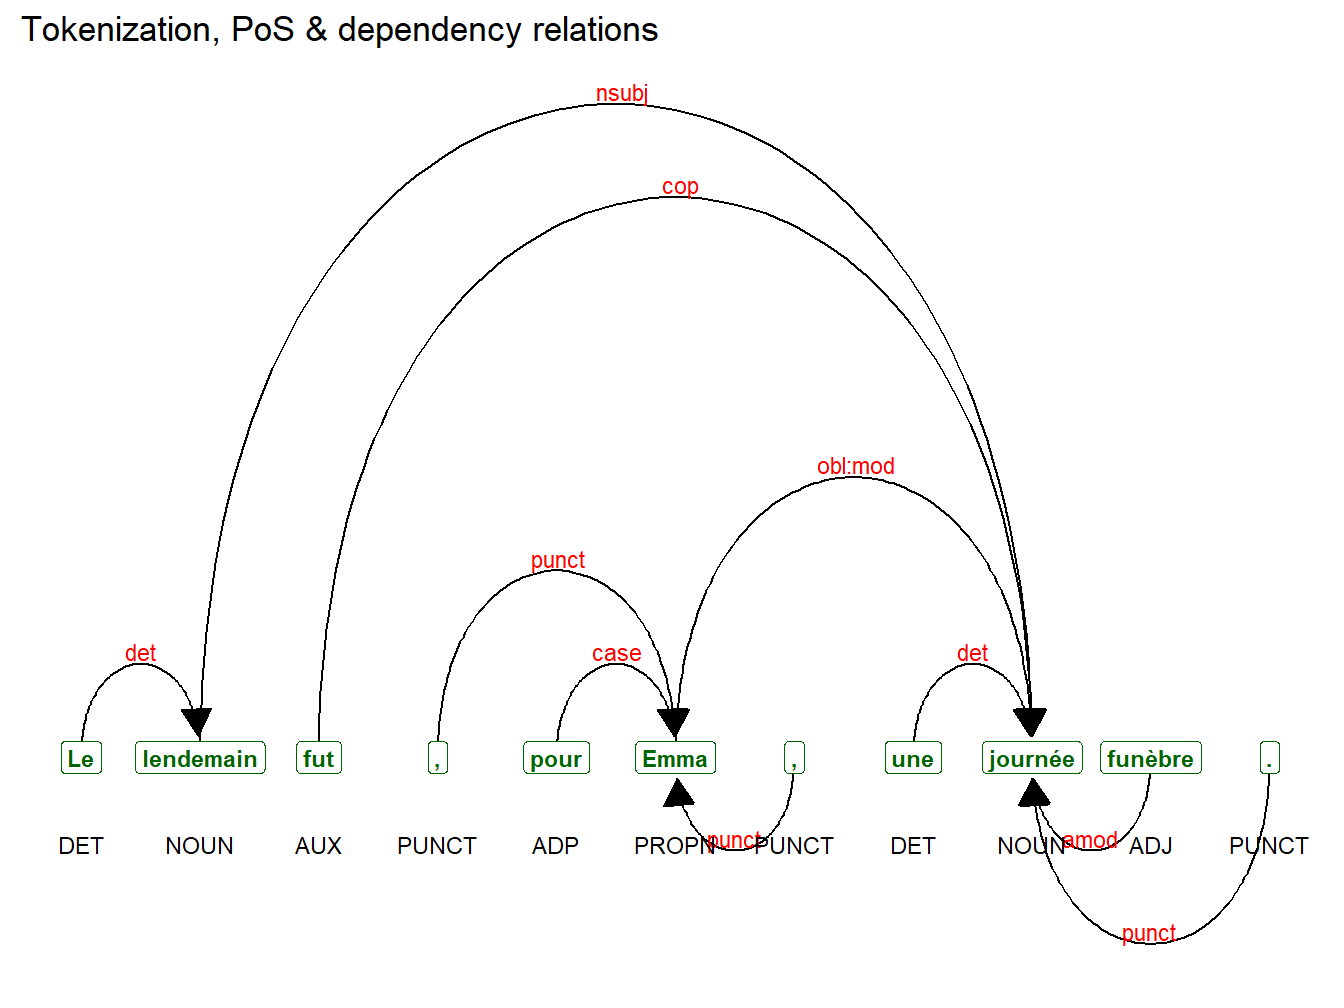
\includegraphics[width=0.8\textwidth,height=\textheight]{q08_Analyse_syntaxic_files/figure-pdf/902-1.pdf}

}

\caption{arbre de dépendance}

\end{figure}%

\subsection{les noms communs et leurs
adjectifs}\label{les-noms-communs-et-leurs-adjectifs}

l'approche facet value

\subsection{les verbes et les actions}\label{les-verbes-et-les-actions}

les verbes et la coordination

l'action dans le langage se manifeste par des formes verbales que
précise certain termes

'' allez vers'' '' lutter contre'', développer l'exemple

\section{Reconnaissance d'entités
nommées}\label{reconnaissance-dentituxe9s-nommuxe9es}

En français courant les entités nommées correspondent largement à l'idée
de noms propres. Un nom propre à une entité. Une chose qui est est
indépendamment des catégories qui peuvent l'étiqueter. John Dupont, né
le 19 février 1898 à Glasgow et abattu à Verdun le 8 août 1917, est un
personnage unique. John Dupont ne désigne par une catégorie, mais bien
une personne singulière. La désignation peut cependant être ambiguë, il
y a un ``Paris, Texas.'', et un Paris sur Seine. La morphologie ne
résout pas l'ambiguïté.

les entités nommées appartiennent à différentes catégories d'objets :
des noms de lieux, des noms de personnes, des noms de marques, des
acronymes d'organisation,

Elles ne représentent jamais une catégorie mais une unité singulière.

des ressources : -
\href{https://cran.r-project.org/web/packages/nametagger/nametagger.pdf}{nametager}
-
\href{https://towardsdatascience.com/quick-guide-to-entity-recognition-and-geocoding-with-r-c0a915932895\%20-\%20\%5Btester\%20cette\%20solution\%20\%5D(https://github.com/trinker/entity/)tester\%20cette\%20solution}{tds}
-\href{https://www.smalsresearch.be/named-entity-recognition-une-application-du-nlp-utile/}{xx}

\section{Co-reférences}\label{co-refuxe9rences}

En linguistique, la co-référence est le phénomène qui consiste pour
plusieurs Syntagme{Groupe de morphèmes ou de mots qui se suivent avec un
sens déterminé (ex. relire, sans s'arrêter).}s nominaux (SN) différents
contenus dans une phrase ou dans un discours, à désigner la même entité.
Par exemple une personne, un lieu, un évènement, ou encore une date.
Dans la terminologie linguistique, on dit qu'une co-référence est reliée
à son antécédent. Pour que les syntagmes se co-réfèrent, les deux
expressions doivent porter les mêmes traits : ils doivent être en accord
en genre, en nombre et en personne.

C'est une tâche difficile, les ressources en français semble inexistante
dans l'univers r.
\href{https://www.rdocumentation.org/packages/cleanNLP/versions/1.9.0/topics/get_coreference}{Une
piste en anglais}

\section{Conclusion}\label{conclusion-6}

La performance des annotateurs. Toute la qualité de l'analyse dépend de
la qualité des annotateurs ? celle ci est généralement bonne au delà des
95\%, mais peut ne pas résister avec certains corpus, Par exemple quand
la ponctuation est absente. Dans ces cas il faut utiliser d'autres
outils qui calculent les ponctuations.

C'est cependant un outil essentiel qui permet de se concentrer sur des
cibles particulières : ce dont on parle, comment on le qualifie, quelles
sont les actions engagées. Il permet d'entrer plus profondément dans la
texture du texte.

\section{Références}\label{ruxe9fuxe9rences}

\bookmarksetup{startatroot}

\chapter{Des tokens à leurs
co-occurences.}\label{des-tokens-uxe0-leurs-co-occurences.}

\begin{Shaded}
\begin{Highlighting}[]
\CommentTok{\#les librairies du chapître}
\FunctionTok{library}\NormalTok{(tidyverse)}
\CommentTok{\#accessoires de ggplot}
\FunctionTok{library}\NormalTok{(ggridges)}
\FunctionTok{library}\NormalTok{(ggrepel)}
\FunctionTok{library}\NormalTok{(ggwordcloud)}
\FunctionTok{library}\NormalTok{(igraph)}
\FunctionTok{library}\NormalTok{(ggraph)}

\FunctionTok{theme\_set}\NormalTok{(}\FunctionTok{theme\_minimal}\NormalTok{()) }

\CommentTok{\#NLP}
\FunctionTok{library}\NormalTok{(tokenizers)}
\FunctionTok{library}\NormalTok{(quanteda)}
\FunctionTok{library}\NormalTok{(quanteda.textplots)}
\FunctionTok{library}\NormalTok{(quanteda.textstats )}

\DocumentationTok{\#\# Analyse de données}
\FunctionTok{library}\NormalTok{(FactoMineR)}
\FunctionTok{library}\NormalTok{(factoextra)}

\CommentTok{\# glossaire}
\FunctionTok{library}\NormalTok{(glossary)}
\FunctionTok{glossary\_path}\NormalTok{(}\StringTok{"glossary.yml"}\NormalTok{)}
\FunctionTok{glossary\_style}\NormalTok{(}\AttributeTok{color =} \StringTok{"purple"}\NormalTok{, }
               \AttributeTok{text\_decoration =} \StringTok{"underline"}\NormalTok{,}
               \AttributeTok{def\_bg =} \StringTok{"\#333"}\NormalTok{,}
               \AttributeTok{def\_color =} \StringTok{"white"}\NormalTok{)}
\end{Highlighting}
\end{Shaded}

\begin{Shaded}
\begin{Highlighting}[]
\FunctionTok{glossary\_popup}\NormalTok{(}\StringTok{"click"}\NormalTok{)}
\CommentTok{\#glossary\_add(term = "hapax", def = "Mot unique dans un corpus donné")}

\CommentTok{\#tableau}
\FunctionTok{library}\NormalTok{(flextable)}
\FunctionTok{set\_flextable\_defaults}\NormalTok{(}
  \AttributeTok{font.size =} \DecValTok{10}\NormalTok{, }\AttributeTok{theme\_fun =}\NormalTok{ theme\_vanilla,}
  \AttributeTok{padding =} \DecValTok{6}\NormalTok{,}
  \AttributeTok{background.color =} \StringTok{"\#EFEFEF"}\NormalTok{)}

\CommentTok{\#palettes}

\FunctionTok{library}\NormalTok{(wesanderson)}
\CommentTok{\#names(wes\_palettes)}
\NormalTok{col\_1}\OtherTok{\textless{}{-}}\FunctionTok{c}\NormalTok{(}\StringTok{"\#85D4E3"}\NormalTok{)}
\NormalTok{col\_1b}\OtherTok{\textless{}{-}}\FunctionTok{c}\NormalTok{(}\StringTok{"\#F4B5BD"}\NormalTok{)}
\NormalTok{col\_2}\OtherTok{\textless{}{-}}\NormalTok{c }\OtherTok{\textless{}{-}}\FunctionTok{c}\NormalTok{(}\StringTok{"\#85D4E3"}\NormalTok{, }\StringTok{"\#F4B5BD"}\NormalTok{)}
\NormalTok{col\_4}\OtherTok{\textless{}{-}}\FunctionTok{c}\NormalTok{(}\StringTok{"\#85D4E3"}\NormalTok{, }\StringTok{"\#F4B5BD"}\NormalTok{, }\StringTok{"\#9C964A"}\NormalTok{, }\StringTok{"\#CDC08C"}\NormalTok{)}
\end{Highlighting}
\end{Shaded}

\textbf{Objectifs du chapitre :}

\emph{Puisque nous savons découper une chaîne de caractères en unités
élémentaires, mais aussi en caractériser la nature (POS,\ldots), nous
allons apprendre à mieux représenter ces éléments sous formes de
tableaux statistiques}

Dans ce chapitre, nous allons travailler sur les textes de MC Solaar,
soit un ensemble de 44 chansons (et rien n'empêche de
\href{https://www.youtube.com/watch?v=22-kiKkc614}{mettre le son}.

\section{Décomposons le pipe}\label{duxe9composons-le-pipe}

\subsection{lire les données et les
sélectionner}\label{lire-les-donnuxe9es-et-les-suxe9lectionner}

On commence par lire le fichier, en apportant des petites corrections.

\begin{Shaded}
\begin{Highlighting}[]
\DocumentationTok{\#\#\#LECTURE du FICHIERS}
\NormalTok{df }\OtherTok{\textless{}{-}} \FunctionTok{read\_csv}\NormalTok{(}\StringTok{"data/RapLyrics.csv"}\NormalTok{, }
    \AttributeTok{locale =} \FunctionTok{locale}\NormalTok{(}\AttributeTok{encoding =} \StringTok{"WINDOWS{-}1252"}\NormalTok{)) }\SpecialCharTok{|\textgreater{}}
  \FunctionTok{filter}\NormalTok{(Artiste}\SpecialCharTok{==}\StringTok{"MC Solaar"}\NormalTok{)}\SpecialCharTok{|\textgreater{}}
  \FunctionTok{mutate}\NormalTok{(}\AttributeTok{Paroles=}\FunctionTok{str\_remove\_all}\NormalTok{(Paroles, }\StringTok{"\textless{}U}\SpecialCharTok{\textbackslash{}\textbackslash{}}\StringTok{+[0{-}9A{-}F]\{4\}\textgreater{}"}\NormalTok{))}
\end{Highlighting}
\end{Shaded}

\subsection{Constituer le corpus}\label{constituer-le-corpus}

On constitue le corpus et on en profites pour examiner les
caractéristiques du texte.

\begin{Shaded}
\begin{Highlighting}[]
\DocumentationTok{\#\#\# création du corpus}
\NormalTok{corpus }\OtherTok{\textless{}{-}} \FunctionTok{corpus}\NormalTok{(df}\SpecialCharTok{$}\NormalTok{Paroles, }\AttributeTok{doc\_var=}\NormalTok{df)  }\CommentTok{\# build a new corpus from the texts}
\NormalTok{summary}\OtherTok{\textless{}{-}}\FunctionTok{as.data.frame}\NormalTok{(}\FunctionTok{summary}\NormalTok{(corpus))}

\NormalTok{summary2}\OtherTok{\textless{}{-}}\FunctionTok{cbind}\NormalTok{(df}\SpecialCharTok{$}\NormalTok{Titre,df}\SpecialCharTok{$}\NormalTok{Date,summary)}\SpecialCharTok{|\textgreater{}}
  \FunctionTok{rename}\NormalTok{(}\AttributeTok{Titre=}\DecValTok{1}\NormalTok{,}
         \AttributeTok{Date=}\DecValTok{2}\NormalTok{)}\SpecialCharTok{|\textgreater{}}
  \FunctionTok{select}\NormalTok{(}\SpecialCharTok{{-}}\NormalTok{Text,}\SpecialCharTok{{-}}\DecValTok{3}\NormalTok{) }\SpecialCharTok{|\textgreater{}}
  \FunctionTok{mutate}\NormalTok{(}\AttributeTok{TTR=}\NormalTok{Types}\SpecialCharTok{/}\NormalTok{Tokens,}
\NormalTok{         complexité}\OtherTok{=}\NormalTok{Tokens}\SpecialCharTok{/}\NormalTok{Sentences,}
         \AttributeTok{Year=}\FunctionTok{year}\NormalTok{(Date)) }\SpecialCharTok{|\textgreater{}}
  \FunctionTok{mutate}\NormalTok{(}\AttributeTok{Titre=}\FunctionTok{str\_remove\_all}\NormalTok{(Titre, }\StringTok{"\textless{}U}\SpecialCharTok{\textbackslash{}\textbackslash{}}\StringTok{+[0{-}9A{-}F]\{4\}\textgreater{}"}\NormalTok{))}

\FunctionTok{ggplot}\NormalTok{(summary2, }\FunctionTok{aes}\NormalTok{(}\AttributeTok{x=}\NormalTok{Year,}\AttributeTok{y=}\NormalTok{TTR))}\SpecialCharTok{+}
  \FunctionTok{geom\_text\_repel}\NormalTok{(}\FunctionTok{aes}\NormalTok{(}\AttributeTok{label=}\NormalTok{Titre), }\AttributeTok{size=}\DecValTok{3}\NormalTok{)}\SpecialCharTok{+}
  \FunctionTok{geom\_smooth}\NormalTok{()}\SpecialCharTok{+} \FunctionTok{labs}\NormalTok{(}\AttributeTok{title=}\StringTok{"Evolution de la diversité du lexique (TTR)"}\NormalTok{)}
\end{Highlighting}
\end{Shaded}

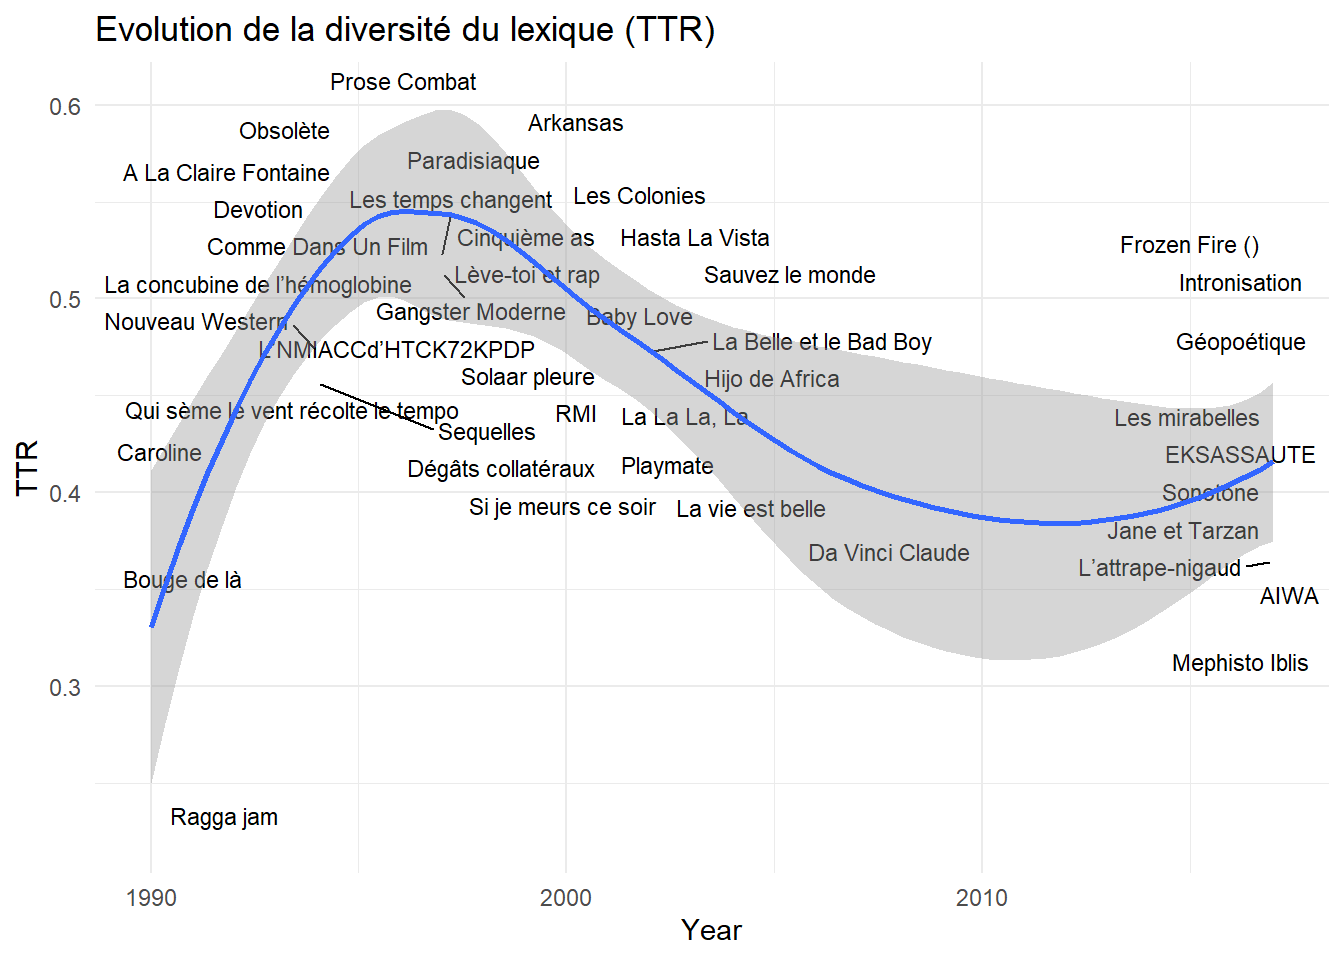
\includegraphics{q09_token_to_dfm_files/figure-pdf/unnamed-chunk-3-1.pdf}

\subsection{tokenizer}\label{tokenizer}

On passe à la tokenisation en nettoyant la ponctuation, les nombres et
les symboles. Ainsi que les stopwords.

\begin{Shaded}
\begin{Highlighting}[]
\CommentTok{\# Créer un dictionnaire de stop words en français}
\NormalTok{stopwords\_fr }\OtherTok{\textless{}{-}} \FunctionTok{stopwords}\NormalTok{(}\StringTok{"fr"}\NormalTok{, }\AttributeTok{source =} \StringTok{"stopwords{-}iso"}\NormalTok{)}

\NormalTok{toks }\OtherTok{\textless{}{-}} \FunctionTok{tokens}\NormalTok{(df}\SpecialCharTok{$}\NormalTok{Paroles,}
               \AttributeTok{remove\_punct =} \ConstantTok{TRUE}\NormalTok{, }
               \AttributeTok{remove\_numbers =} \ConstantTok{TRUE}\NormalTok{, }
               \AttributeTok{remove\_symbols =} \ConstantTok{TRUE}\NormalTok{) }\SpecialCharTok{|\textgreater{}}
  \FunctionTok{tokens\_remove}\NormalTok{(}\AttributeTok{pattern =}\NormalTok{ stopwords\_fr)}

\FunctionTok{head}\NormalTok{(toks)}
\end{Highlighting}
\end{Shaded}

\begin{verbatim}
Tokens consisting of 6 documents.
text1 :
 [1] "Fuck"      "Terre"     "meurs"     "testament" "Déposez"   "cendres"  
 [7] "bouche"    "opposants" "Virez"     "coup"      "d'front"   "kick"     
[ ... and 360 more ]

text2 :
 [1] "J'étais"    "cool"       "assis"      "banc"       "c'était"   
 [6] "printemps"  "cueillent"  "marguerite" "amants"     "Overdose"  
[11] "douceur"    "jouent"    
[ ... and 211 more ]

text3 :
 [1] "s'étaient"  "rencontrés" "bancs"      "d'l'école"  "heure"     
 [6] "colle"      "maths"      "cours"      "d'espagnol" "C'était"   
[11] "fille"      "fun"       
[ ... and 160 more ]

text4 :
 [1] "passe-t-il" "c'est"      "personnel"  "douleur"    "éternelle" 
 [6] "partageais" "qu'avec"    "ciel"       "monstre"    "yeux"      
[11] "verts"      "synonyme"  
[ ... and 215 more ]

text5 :
 [1] "Hasta"      "siempre"    "viva"       "Revolucion" "Rapero"    
 [6] "numero"     "uno"        "el"         "grito"      "cancion"   
[11] "Soy"        "el"        
[ ... and 202 more ]

text6 :
 [1] "vie"        "belle"      "vie"        "belle"      "vie"       
 [6] "belle"      "chambre"    "jour"       "normal"     "J'apprends"
[11] "journaux"   "j'suis"    
[ ... and 287 more ]
\end{verbatim}

\subsection{\texorpdfstring{Construire le
\texttt{dfm}}{Construire le dfm}}\label{construire-le-dfm}

Les tokens sont dans quanteda une liste de mots associés à chaque texte.
En l'Etat ils ne peuvent être exploités directement. On aura besoin dans
les analyses ultérieures de les recomposer sous la forme d'un tableau
texte x mots, dans lequel chaque cellule représente le nombre de fois où
un mot est employé dans un texte.

Des outils tels que \texttt{quanteda}, simplifie la tâche en proposant
une fonction qui fait l'opération simplement en une fonction
élémentaire. Cette matrice que nous appelons \texttt{dfm} pour document
feature matrix (les matrices peuvent êtres des mots ou d'autres termes
comme des collocations) , possède une particularité : c'est une matrice
creuse, ou vide, la plus part de ses éléments sont égaux à zéro.

\begin{Shaded}
\begin{Highlighting}[]
\NormalTok{dfm}\OtherTok{\textless{}{-}}\FunctionTok{dfm}\NormalTok{(toks)}

\FunctionTok{head}\NormalTok{(dfm)}
\end{Highlighting}
\end{Shaded}

\begin{verbatim}
Document-feature matrix of: 6 documents, 4,876 features (96.28% sparse) and 0 docvars.
       features
docs    fuck terre meurs testament déposez cendres bouche opposants virez coup
  text1    1     4     1         1       1       1      1         1     1    1
  text2    0     0     0         0       0       0      0         0     0    0
  text3    0     0     0         0       0       0      0         0     0    0
  text4    0     0     0         0       0       0      0         0     0    0
  text5    0     0     0         0       0       0      0         0     0    0
  text6    0     0     0         0       0       0      0         0     0    0
[ reached max_nfeat ... 4,866 more features ]
\end{verbatim}

Pour mieux s'en représenter le contenu, un petit nuage de mots fera
l'affaire. On sélectionne ceux qui ont été employés au moins cinq fois.

\begin{Shaded}
\begin{Highlighting}[]
\NormalTok{dfm\_df}\OtherTok{\textless{}{-}}\FunctionTok{convert}\NormalTok{(dfm, }\AttributeTok{to=}\StringTok{"data.frame"}\NormalTok{)}

\NormalTok{foo1}\OtherTok{\textless{}{-}} \FunctionTok{cbind}\NormalTok{(summary2}\SpecialCharTok{$}\NormalTok{Titre, dfm\_df) }\SpecialCharTok{|\textgreater{}}
  \FunctionTok{rename}\NormalTok{(}\AttributeTok{Titre=}\DecValTok{1}\NormalTok{)}\SpecialCharTok{|\textgreater{}}
  \FunctionTok{select}\NormalTok{(}\SpecialCharTok{{-}}\NormalTok{doc\_id)}\SpecialCharTok{|\textgreater{}}
  \FunctionTok{pivot\_longer}\NormalTok{(}\SpecialCharTok{{-}}\NormalTok{Titre, }\AttributeTok{names\_to =} \StringTok{"Tokens"}\NormalTok{, }\AttributeTok{values\_to =} \StringTok{"Fréquence"}\NormalTok{) }\SpecialCharTok{|\textgreater{}}
    \FunctionTok{group\_by}\NormalTok{(Tokens)}\SpecialCharTok{|\textgreater{}}
  \FunctionTok{summarise}\NormalTok{(Fréquence}\OtherTok{=}\FunctionTok{sum}\NormalTok{(Fréquence)) }\SpecialCharTok{|\textgreater{}}
  \FunctionTok{filter}\NormalTok{( Fréquence}\SpecialCharTok{\textgreater{}}\DecValTok{5}\NormalTok{)}

\NormalTok{n}\OtherTok{\textless{}{-}}\FunctionTok{nrow}\NormalTok{(foo1)}
\FunctionTok{set.seed}\NormalTok{(}\DecValTok{42}\NormalTok{)}
\FunctionTok{ggplot}\NormalTok{(foo1, }\FunctionTok{aes}\NormalTok{(}\AttributeTok{label =}\NormalTok{ Tokens, }\AttributeTok{size =}\NormalTok{ Fréquence)) }\SpecialCharTok{+}
  \FunctionTok{geom\_text\_wordcloud}\NormalTok{(}\FunctionTok{aes}\NormalTok{(}\AttributeTok{color=}\NormalTok{Fréquence)) }\SpecialCharTok{+}
  \FunctionTok{scale\_size\_area}\NormalTok{(}\AttributeTok{max\_size =} \DecValTok{12}\NormalTok{) }\SpecialCharTok{+}
  \FunctionTok{theme\_minimal}\NormalTok{()}\SpecialCharTok{+}
  \FunctionTok{scale\_color\_gradient}\NormalTok{(}\AttributeTok{low =} \StringTok{"brown"}\NormalTok{, }\AttributeTok{high =} \StringTok{"red"}\NormalTok{)}
\end{Highlighting}
\end{Shaded}

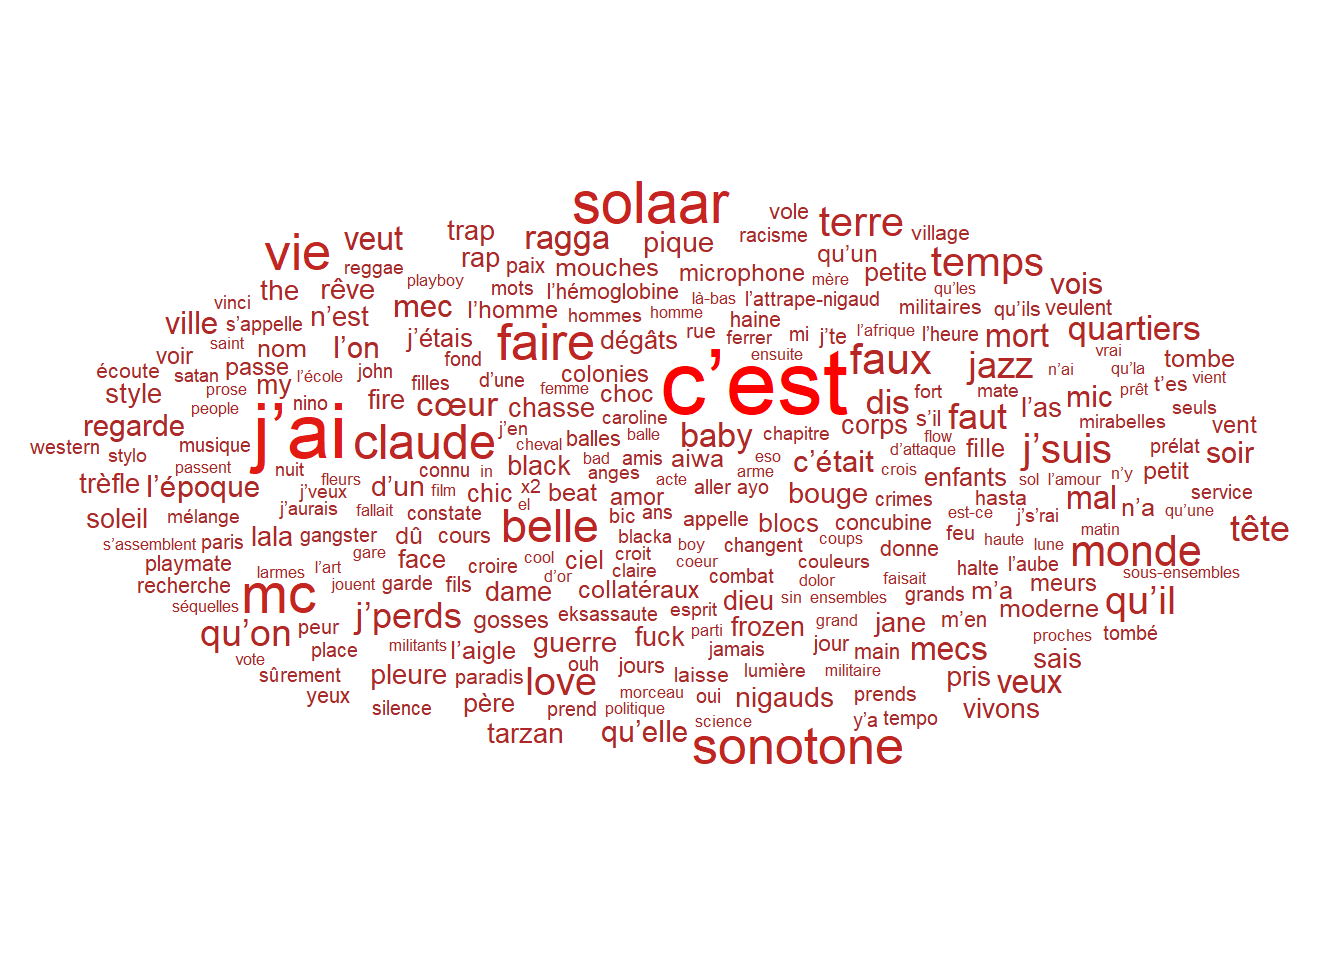
\includegraphics{q09_token_to_dfm_files/figure-pdf/unnamed-chunk-6-1.pdf}

\begin{Shaded}
\begin{Highlighting}[]
\NormalTok{foo}\OtherTok{\textless{}{-}} \FunctionTok{cbind}\NormalTok{(summary2}\SpecialCharTok{$}\NormalTok{Titre, dfm\_df) }\SpecialCharTok{|\textgreater{}}
  \FunctionTok{rename}\NormalTok{(}\AttributeTok{Titre=}\DecValTok{1}\NormalTok{)}\SpecialCharTok{|\textgreater{}}
  \FunctionTok{select}\NormalTok{(}\SpecialCharTok{{-}}\NormalTok{doc\_id)}\SpecialCharTok{|\textgreater{}}
  \FunctionTok{pivot\_longer}\NormalTok{(}\SpecialCharTok{{-}}\NormalTok{Titre, }\AttributeTok{names\_to =} \StringTok{"Tokens"}\NormalTok{, }\AttributeTok{values\_to =} \StringTok{"Fréquence"}\NormalTok{) }\SpecialCharTok{|\textgreater{}}
    \FunctionTok{group\_by}\NormalTok{(Tokens)}\SpecialCharTok{|\textgreater{}}
  \FunctionTok{summarise}\NormalTok{(Fréquence}\OtherTok{=}\FunctionTok{sum}\NormalTok{(Fréquence)) }\SpecialCharTok{|\textgreater{}}
  \FunctionTok{filter}\NormalTok{( Fréquence}\SpecialCharTok{\textless{}}\DecValTok{2}\NormalTok{)}
\NormalTok{l}\OtherTok{\textless{}{-}}\FunctionTok{nrow}\NormalTok{(foo)}

\NormalTok{foo}\OtherTok{\textless{}{-}} \FunctionTok{cbind}\NormalTok{(summary2}\SpecialCharTok{$}\NormalTok{Titre, dfm\_df) }\SpecialCharTok{|\textgreater{}}
  \FunctionTok{rename}\NormalTok{(}\AttributeTok{Titre=}\DecValTok{1}\NormalTok{)}\SpecialCharTok{|\textgreater{}}
  \FunctionTok{select}\NormalTok{(}\SpecialCharTok{{-}}\NormalTok{doc\_id)}\SpecialCharTok{|\textgreater{}}
  \FunctionTok{pivot\_longer}\NormalTok{(}\SpecialCharTok{{-}}\NormalTok{Titre, }\AttributeTok{names\_to =} \StringTok{"Tokens"}\NormalTok{, }\AttributeTok{values\_to =} \StringTok{"Fréquence"}\NormalTok{) }\SpecialCharTok{|\textgreater{}}
    \FunctionTok{group\_by}\NormalTok{(Tokens)}\SpecialCharTok{|\textgreater{}}
  \FunctionTok{summarise}\NormalTok{(Fréquence}\OtherTok{=}\FunctionTok{sum}\NormalTok{(Fréquence)) }\SpecialCharTok{|\textgreater{}}
  \FunctionTok{filter}\NormalTok{( Fréquence}\SpecialCharTok{\textgreater{}}\DecValTok{1}\NormalTok{)}
\NormalTok{m}\OtherTok{\textless{}{-}}\FunctionTok{nrow}\NormalTok{(foo)}
\end{Highlighting}
\end{Shaded}

A ce stade on dispose d'un tableau textes x mots de dimension
{[}44,5800{]} dont la grande part sont des hapax{Mot unique dans un
corpus donné} , on en compte 3522. Ils sont 1354 à être répété plus
d'une fois, et 270 6 fois et plus.

En voici une image condensée.

\begin{Shaded}
\begin{Highlighting}[]
\NormalTok{df\_afc }\OtherTok{\textless{}{-}} \FunctionTok{cbind}\NormalTok{(summary2}\SpecialCharTok{$}\NormalTok{Titre, dfm\_df) }\SpecialCharTok{|\textgreater{}}
  \FunctionTok{rename}\NormalTok{(}\AttributeTok{Titre=}\DecValTok{1}\NormalTok{)}\SpecialCharTok{|\textgreater{}}
  \FunctionTok{select}\NormalTok{(}\SpecialCharTok{{-}}\NormalTok{doc\_id)}\SpecialCharTok{|\textgreater{}}
  \FunctionTok{pivot\_longer}\NormalTok{(}\SpecialCharTok{{-}}\NormalTok{Titre, }\AttributeTok{names\_to =} \StringTok{"Tokens"}\NormalTok{, }\AttributeTok{values\_to =} \StringTok{"Fréquence\_text"}\NormalTok{) }\SpecialCharTok{|\textgreater{}}
    \FunctionTok{group\_by}\NormalTok{(Titre, Tokens)}\SpecialCharTok{|\textgreater{}}
  \FunctionTok{summarise}\NormalTok{(Fréquence}\AttributeTok{\_text=}\FunctionTok{sum}\NormalTok{(Fréquence\_text))}\SpecialCharTok{|\textgreater{}}
  \FunctionTok{ungroup}\NormalTok{()}\SpecialCharTok{|\textgreater{}}
  \FunctionTok{left\_join}\NormalTok{(foo1)}\SpecialCharTok{|\textgreater{}}
  \FunctionTok{filter}\NormalTok{(}\SpecialCharTok{!}\FunctionTok{is.na}\NormalTok{(Fréquence))}

\NormalTok{foo}\OtherTok{\textless{}{-}}\NormalTok{ df\_afc}\SpecialCharTok{|\textgreater{}}
  \FunctionTok{filter}\NormalTok{(Fréquence}\SpecialCharTok{\textgreater{}}\DecValTok{15}\NormalTok{)}

\FunctionTok{ggplot}\NormalTok{(foo, }\FunctionTok{aes}\NormalTok{(Titre, Tokens, }\AttributeTok{fill =}\NormalTok{ Fréquence\_text)) }\SpecialCharTok{+}
  \FunctionTok{geom\_tile}\NormalTok{() }\SpecialCharTok{+}
  \FunctionTok{scale\_fill\_gradient}\NormalTok{(}\AttributeTok{low =} \StringTok{"white"}\NormalTok{, }\AttributeTok{high =} \StringTok{"grey10"}\NormalTok{) }\SpecialCharTok{+}
  \FunctionTok{theme\_minimal}\NormalTok{() }\SpecialCharTok{+}
  \FunctionTok{theme}\NormalTok{(}
    \AttributeTok{axis.text.x =} \FunctionTok{element\_text}\NormalTok{(}\AttributeTok{angle =} \DecValTok{60}\NormalTok{, }\AttributeTok{vjust =} \DecValTok{1}\NormalTok{, }\AttributeTok{size =} \DecValTok{7}\NormalTok{, }\AttributeTok{hjust =} \DecValTok{1}\NormalTok{),}
    \AttributeTok{axis.text.y =} \FunctionTok{element\_text}\NormalTok{(}\AttributeTok{size =} \DecValTok{7}\NormalTok{),}
    \AttributeTok{axis.title.x =} \FunctionTok{element\_blank}\NormalTok{(),}
    \AttributeTok{axis.title.y =} \FunctionTok{element\_blank}\NormalTok{()}
\NormalTok{  ) }\SpecialCharTok{+}
  \FunctionTok{labs}\NormalTok{(}\AttributeTok{fill =} \StringTok{"Value"}\NormalTok{)}
\end{Highlighting}
\end{Shaded}

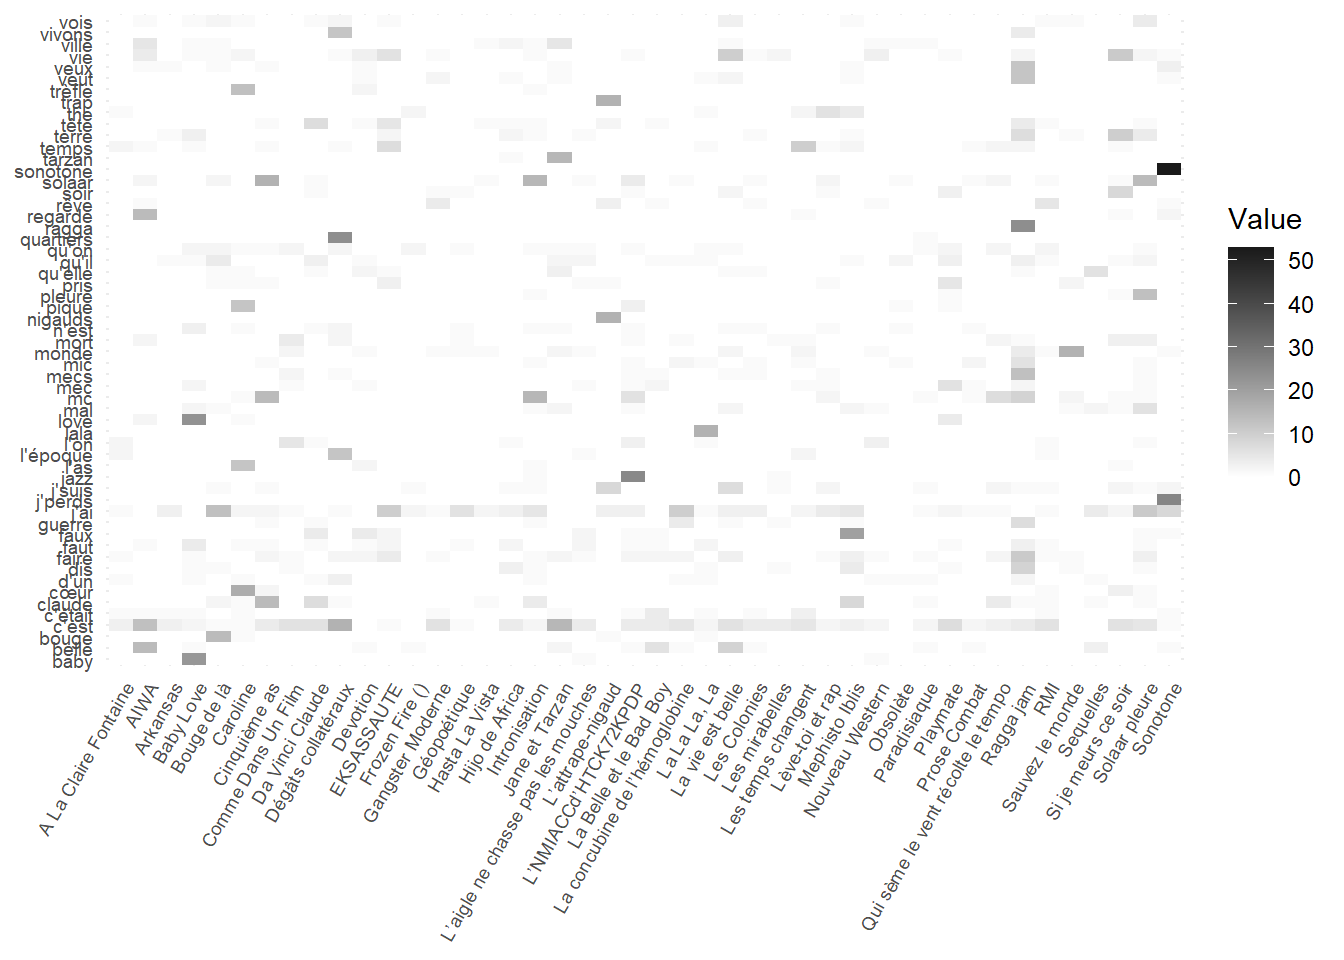
\includegraphics{q09_token_to_dfm_files/figure-pdf/unnamed-chunk-7-1.pdf}

\begin{Shaded}
\begin{Highlighting}[]
\NormalTok{df\_AFC}\OtherTok{\textless{}{-}}\NormalTok{df\_afc }\SpecialCharTok{\%\textgreater{}\%}
  \FunctionTok{select}\NormalTok{(}\SpecialCharTok{{-}}\NormalTok{Fréquence) }\SpecialCharTok{|\textgreater{}}
  \FunctionTok{pivot\_wider}\NormalTok{(}\AttributeTok{id\_cols=}\NormalTok{Tokens, }\AttributeTok{names\_from =} \StringTok{"Titre"}\NormalTok{, }\AttributeTok{values\_from =} \StringTok{"Fréquence\_text"}\NormalTok{)}\SpecialCharTok{\%\textgreater{}\%}
  \FunctionTok{column\_to\_rownames}\NormalTok{(}\AttributeTok{var=}\StringTok{"Tokens"}\NormalTok{)}

\FunctionTok{head}\NormalTok{(df\_AFC[,}\DecValTok{1}\SpecialCharTok{:}\DecValTok{6}\NormalTok{])}
\end{Highlighting}
\end{Shaded}

\begin{verbatim}
      A La Claire Fontaine AIWA Arkansas Baby Love Bouge de là Caroline
acte                     0    0        0         0           0        0
aiwa                     0   12        0         0           0        0
aller                    0    0        0         0           1        0
amis                     0    0        0         0           1        0
amor                     0    0        0         0           0        0
anges                    0    0        0         0           0        0
\end{verbatim}

\subsection{Son analyse par la vénérable
AFC}\label{son-analyse-par-la-vuxe9nuxe9rable-afc}

L' Analyse factorielle des Correspondance, héritage de Benzecri (2006),
est l'outil traditionnel de l'analyse textuelle et de ce type de
tableau. Elle permet de donner une représentation des lignes et des
colonnes, des mots et des textes, simultanément.

\begin{Shaded}
\begin{Highlighting}[]
\NormalTok{res.ca }\OtherTok{\textless{}{-}} \FunctionTok{CA}\NormalTok{(df\_AFC, }\AttributeTok{graph =} \ConstantTok{FALSE}\NormalTok{)}
\CommentTok{\#fviz\_screeplot(res.ca, addlabels = TRUE, ylim = c(0, 10))}

\NormalTok{d\_word}\OtherTok{\textless{}{-}}\FunctionTok{as.data.frame}\NormalTok{(res.ca}\SpecialCharTok{$}\NormalTok{row}\SpecialCharTok{$}\NormalTok{coord) }\SpecialCharTok{\%\textgreater{}\%}
  \FunctionTok{rownames\_to\_column}\NormalTok{(}\AttributeTok{var=}\StringTok{"Tokens"}\NormalTok{) }\SpecialCharTok{|\textgreater{}}
  \FunctionTok{left\_join}\NormalTok{(foo1) }\SpecialCharTok{\%\textgreater{}\%}\FunctionTok{filter}\NormalTok{(Fréquence}\SpecialCharTok{\textgreater{}}\DecValTok{10}\NormalTok{)}

\NormalTok{d\_texte}\OtherTok{\textless{}{-}}\FunctionTok{as.data.frame}\NormalTok{(res.ca}\SpecialCharTok{$}\NormalTok{col}\SpecialCharTok{$}\NormalTok{coord)}\SpecialCharTok{\%\textgreater{}\%}
  \FunctionTok{rownames\_to\_column}\NormalTok{(}\AttributeTok{var=}\StringTok{"Tokens"}\NormalTok{) }\SpecialCharTok{|\textgreater{}}
  \FunctionTok{mutate}\NormalTok{(Fréquence}\OtherTok{=}\DecValTok{10}\NormalTok{)}

\NormalTok{ca}\OtherTok{\textless{}{-}}\FunctionTok{rbind}\NormalTok{(d\_word,d\_texte) }\SpecialCharTok{\%\textgreater{}\%}
  \FunctionTok{mutate}\NormalTok{(}\AttributeTok{Type=}\FunctionTok{ifelse}\NormalTok{(Fréquence}\SpecialCharTok{==}\DecValTok{10}\NormalTok{,}\StringTok{"texte"}\NormalTok{, }\StringTok{"word"}\NormalTok{))}

\FunctionTok{ggplot}\NormalTok{(ca, }\FunctionTok{aes}\NormalTok{(}\AttributeTok{x=}\StringTok{\textasciigrave{}}\AttributeTok{Dim 1}\StringTok{\textasciigrave{}}\NormalTok{, }\AttributeTok{y=}\StringTok{\textasciigrave{}}\AttributeTok{Dim 2}\StringTok{\textasciigrave{}}\NormalTok{, }\AttributeTok{color=}\NormalTok{Type))}\SpecialCharTok{+}
  \FunctionTok{geom\_text\_repel}\NormalTok{(}\FunctionTok{aes}\NormalTok{(}\AttributeTok{label=}\NormalTok{Tokens), }\AttributeTok{size=}\DecValTok{2}\NormalTok{, }\AttributeTok{max.overlaps =}\DecValTok{80}\NormalTok{)}\SpecialCharTok{+}
  \FunctionTok{theme}\NormalTok{(}
    \AttributeTok{axis.text.x =} \FunctionTok{element\_text}\NormalTok{(}\AttributeTok{angle =} \DecValTok{45}\NormalTok{, }\AttributeTok{vjust =} \DecValTok{1}\NormalTok{, }\AttributeTok{size =} \DecValTok{8}\NormalTok{, }\AttributeTok{hjust =} \DecValTok{1}\NormalTok{),}
    \AttributeTok{axis.text.y =} \FunctionTok{element\_text}\NormalTok{(}\AttributeTok{size =} \DecValTok{8}\NormalTok{),}
    \AttributeTok{axis.title.x =} \FunctionTok{element\_blank}\NormalTok{(),}
    \AttributeTok{axis.title.y =} \FunctionTok{element\_blank}\NormalTok{()}
\NormalTok{  ) }\CommentTok{\#+ylim({-}2,1)+xlim({-}1,1)}
\end{Highlighting}
\end{Shaded}

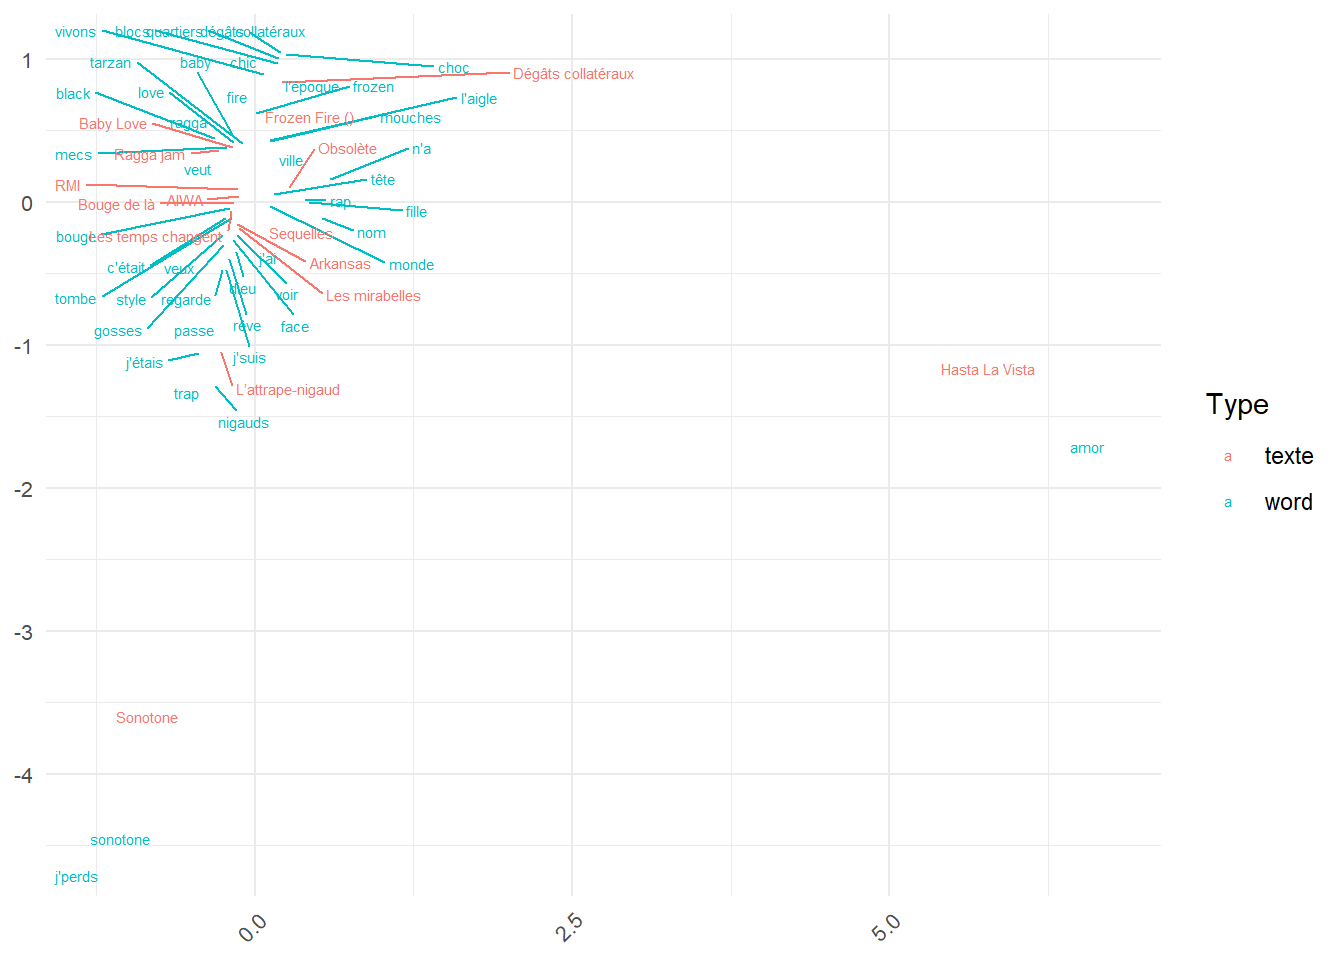
\includegraphics{q09_token_to_dfm_files/figure-pdf/unnamed-chunk-8-1.pdf}

Nous verrons dans le chapitre suivant des méthodes bien plus efficace.

\section{Tf-idf}\label{tf-idf}

Le dfm a un défaut, il ne tient pas compte du fait que les mots
fréquents peuvent être partagés par un grand nombre de texte et
n'indiquer rien d'autre qu'un élément régulier du corpus, un plus petit
dénominateur commun, des mots un peu moins fréquents mais concentrés sur
quelques textes sont plus informatifs.

C'est cette idée qui conduit à une autre métrique, celle du Tf-idf qui
pondère la fréquence d'un mot dans un texte par l'inverse de sa
fréquence dans les documents. Les mots qu'on retrouvent partout sont
pénalisés.

Dans un \emph{dfm}, chaque cellule du tableau indique la fréquence d'un
mot dans un document. Cette mesure cependant peut ne pas être
pertinentes. Les mots les plus fréquents peuvent se distribuer également
entre les documents, et leur fréquence indique au mieux un lieu commun.

L'idée clé va être de pondérer la fréquence d'un terme dans un document
par la présence de ce terme à travers les documents. S'il se retrouve
partout on en minore le poids, s'ils est présent dans une petit groupe
de document on va lui donner de l'importance.

\subsection{le calcul}\label{le-calcul}

Le TF-IDF est calculé en deux étapes :

\begin{enumerate}
\def\labelenumi{\arabic{enumi}.}
\tightlist
\item
  \textbf{Term Frequency (TF)} : La fréquence d'un terme \(t\) dans un
  document \(d\) est définie par :\(f_{td}\)
\end{enumerate}

\(TF_{t,d} = \frac{f_{td}}{f_{.d}}\)

\begin{enumerate}
\def\labelenumi{\arabic{enumi}.}
\setcounter{enumi}{1}
\tightlist
\item
  \textbf{Inverse Document Frequency (IDF)} : L'IDF d'un terme ( t )
  dans un corpus de documents est donnée par :
\end{enumerate}

\(IDF_{t} = \log (\frac{D}{D_t} )\)

Le TF-IDF est alors le produit du TF et de l'IDF :

\$ \text{TF-IDF}(t, d) = \text{TF}(t, d) \times \text{IDF}(t)\$

\subsection{les variantes}\label{les-variantes}

\subsection{On met en oeuvre}\label{on-met-en-oeuvre}

\subsection{le concept de tfidf}\label{le-concept-de-tfidf}

Cette idée est formalisée par le critère du TfIdf. La fréquence d'un
terme dans un document (Tf) par être pondéré par l'inverse de la
fréquence des documents dans lesquels il est présent (Idf). S'il est
présent partout (c'est le cas des verbes auxiliaires) sont poids sera
minimal, s'il est concentré dans un petit nombre de documents on lui
donnera un poids plus important.

Formalisation

la fréquence brute des termes est le rapport du nombre de termes i dans
le document d sur le nombre de termes du document i

\(tf_{id}= n_{id}\)

Cette fréquence peut être modulée par le nombre de mots dans le texte,
cette fréquence relative permet d'avoir une idée de la densité d'un
terme dans un document.

\(tf_{id}= n_{id}/\sum_{i}(n_{id})\)

la pondération

\(idf_{id}= log(D_{}/D_{i})\)

Ce concept souligne une chose capitale : un terme, ou token, dans un
corpus, est caractérisé par une double distribution : d'une part sa part
dans l'ensemble des termes de références, et d'autre part, sa présence à
travers les documents.

\subsection{D'autres variantes}\label{dautres-variantes}

Celles de l'idf
\url{https://programminghistorian.org/fr/lecons/analyse-de-documents-avec-tfidf}

le bm25 est une généralisation à une requête Q de plusieurs termes et
vise à qualifier la pertinence

on développe avec une étude empirique.

\section{Calculer les coocurrences}\label{calculer-les-coocurrences}

\subsection{Un simple exemple}\label{un-simple-exemple}

on continue avec quanteda.

\subsection{Des mesures plus
sensibles}\label{des-mesures-plus-sensibles}

les co-occurrences peuvent être calculées sur une fenêtre de texte. Deux
mots ne sont pas forcément similaires s'ils sont dans le même texte, il
le sont plus s'ils sont employés dans la même séquence de texte, dans
une même fenêtre. C'est une manière de prendre mieux en compte le
contexte, cette notion essentielle pour identifier le sens des termes :
il est lié à leur proximités aux autres termes de leur contexte. Le sens
des mots se déterminent par leurs usages communs.

\subsection{ou des distances}\label{ou-des-distances}

\section{Références}\label{ruxe9fuxe9rences-1}

\bookmarksetup{startatroot}

\chapter{Analyse des co-occurrences}\label{analyse-des-co-occurrences}

\begin{Shaded}
\begin{Highlighting}[]
\CommentTok{\#les librairies du chapitre}
\FunctionTok{library}\NormalTok{(tidyverse)}
\FunctionTok{library}\NormalTok{(readr)}
\FunctionTok{library}\NormalTok{(tokenizers)}
\FunctionTok{library}\NormalTok{(quanteda)}
\FunctionTok{library}\NormalTok{(quanteda.textplots)}
\FunctionTok{library}\NormalTok{(flextable)}


\CommentTok{\# glossaire}
\FunctionTok{library}\NormalTok{(glossary)}
\FunctionTok{glossary\_path}\NormalTok{(}\StringTok{"glossary.yml"}\NormalTok{)}
\FunctionTok{glossary\_style}\NormalTok{(}\AttributeTok{color =} \StringTok{"purple"}\NormalTok{, }
               \AttributeTok{text\_decoration =} \StringTok{"underline"}\NormalTok{,}
               \AttributeTok{def\_bg =} \StringTok{"\#333"}\NormalTok{,}
               \AttributeTok{def\_color =} \StringTok{"white"}\NormalTok{)}
\end{Highlighting}
\end{Shaded}

\begin{verbatim}
<style>
a.glossary {
  color: purple;
  text-decoration: underline;
  cursor: help;
  position: relative;
}

/* only needed for popup = "click" */
/* popup-definition */
a.glossary .def {
  display: none;
  position: absolute;
  z-index: 1;
  width: 200px;
  bottom: 100%;
  left: 50%;
  margin-left: -100px;
  background-color: #333;
  color: white;
  padding: 5px;
  border-radius: 6px;
}
/* show on click */
a.glossary:active .def {
  display: inline-block;
}
/* triangle arrow */
a.glossary:active .def::after {
  content: ' ';
  position: absolute;
  top: 100%;
  left: 50%;
  margin-left: -5px;
  border-width: 5px;
  border-style: solid;
  border-color: #333 transparent transparent transparent;
}
</style>
\end{verbatim}

\begin{Shaded}
\begin{Highlighting}[]
\CommentTok{\#theme setting}
\FunctionTok{theme\_set}\NormalTok{(}\FunctionTok{theme\_minimal}\NormalTok{()) }

\FunctionTok{set\_flextable\_defaults}\NormalTok{(}
  \AttributeTok{font.size =} \DecValTok{10}\NormalTok{, }\AttributeTok{theme\_fun =}\NormalTok{ theme\_vanilla,}
  \AttributeTok{padding =} \DecValTok{6}\NormalTok{,}
  \AttributeTok{background.color =} \StringTok{"\#EFEFEF"}\NormalTok{)}
\end{Highlighting}
\end{Shaded}

\textbf{Objectifs du chapitre :}

\emph{Jusqu'à présent, nous nous sommes consacrés au traitement des
chaines de caractères, généralement dans un but univarié, examinant la
distribution des termes.}

\emph{Ce chapitre est celui d'un virage multivarié : ce qu'on va étudier
ce sont les distributions conjointes des termes, au travers
principalement de l'analyse de leur co-occurrences. On découvrira une
large palette de techniques qui permettent de les représenter et
d'identifier des thématique et la manières dont elles s'articulent.
Elles sont principalement descriptive.}

A ce stade nous arrivons à la question de l'analyse des co-occurences.

Dans quelle mesures deux termes se retrouvent souvent ensemble c'est à
dire dans le même contexte?

C'est à dire l'analyse d'une matrice de similarités entre un grand
nombre d'objets,

\section{Des co-occurences aux
similarités}\label{des-co-occurences-aux-similarituxe9s}

On continue avec la boite à outil quanteda

On peut naturellement faire varier les critères de cooccurence en
définition la fen\^{}rtre commune de deux mots. Au lieu de prendre
l'ensemble du texte.

Un tel tableau est un tableau de similarité, et il sera généralement
utile de traiter un tableau de dis-similarités.

Une

\section{Approche par classification
hiérarchique}\label{approche-par-classification-hiuxe9rarchique}

Une approche évidente de ce type d'objet est celle des méthodes de
classification hiérarchiques dont il faut rappeler l'origine
biologiques. Dans le problèmes de la construction d'un arbre
évolutionnaire des espèces ou des variétés, la méthode générale s'appuie
sur le calcul de distances, qui peuvent être phénotypiques, ou
génomiques.

\subsection{Un peu d'histoire et de
théorie}\label{un-peu-dhistoire-et-de-thuxe9orie}

sur ce plan On doit beaucoup à sokal et sneath

https://www.amazon.com/Principles-Numerical-Taxonomy-Robert-Sneath/dp/B009SA478O

pour un commentaire, car celà appartient à l'histoire des sciences

https://www.jstor.org/stable/4026976

Ces méthodes généralement différent par deux critère

le mode de clacul de la distance

la méthode d'agrgation

\subsection{Un exemple simple}\label{un-exemple-simple}

\subsection{Des variantes pertinentes relativement au
texte}\label{des-variantes-pertinentes-relativement-au-texte}

les approches descendantes ( et les arbres de décision) rheinhart

dbscan de bertopic

\section{Cartes de positionnement}\label{cartes-de-positionnement}

Le problème de la représentation des distance entre un certain nombres
de point est abordé depuis longtemps par les méthodes d'analyses de
similarités, qui cependant n'étaient pas forcément adaptées au
traitement d'un grand nombre d'objets. Des méthodes de forces ont été
introduites notamment pour résoudre les problème de visualisation.
Aujourd'hui deux méthodes ce sont imposée et sont les standards dans les
domaines du texte, ou les termes sont très nombreux. Il s'agit de Tsne
et d'Umap.

\subsection{MDS et PCA}\label{mds-et-pca}

\begin{enumerate}
\def\labelenumi{\arabic{enumi}.}
\item
  Torgerson, Warren S. (1958). \emph{Theory \& Methods of Scaling}. New
  York: Wiley.
  \href{https://en.wikipedia.org/wiki/ISBN_(identifier)}{ISBN}~\href{https://en.wikipedia.org/wiki/Special:BookSources/978-0-89874-722-5}{978-0-89874-722-5}.
\item
\item
  \href{https://en.wikipedia.org/wiki/Joseph_Kruskal}{Kruskal, J. B.}
  (1964). ``Multidimensional scaling by optimizing goodness of fit to a
  nonmetric hypothesis''. \emph{Psychometrika}. \textbf{29} (1): 1--27.
  \href{https://en.wikipedia.org/wiki/Doi_(identifier)}{doi}:\href{https://doi.org/10.1007\%2FBF02289565}{10.1007/BF02289565}.
  \href{https://en.wikipedia.org/wiki/S2CID_(identifier)}{S2CID}~\href{https://api.semanticscholar.org/CorpusID:48165675}{48165675}.
\item
  Mead, A (1992). ``Review of the Development of Multidimensional
  Scaling Methods''. \emph{Journal of the Royal Statistical Society.
  Series D (The Statistician)}. \textbf{41} (1): 27--39.
  \href{https://en.wikipedia.org/wiki/JSTOR_(identifier)}{JSTOR}~\href{https://www.jstor.org/stable/2348634}{2348634}.
  Abstract. Multidimensional scaling methods are now a common
  statistical tool in psychophysics and sensory analysis. The
  development of these methods is charted, from the original research of
  Torgerson (metric scaling), Shepard and Kruskal (non-metric scaling)
  through individual differences scaling and the maximum likelihood
  methods proposed by Ramsay.
\item
  Green, P. (January 1975). ``Marketing applications of MDS: Assessment
  and outlook''. \emph{Journal of Marketing}. \textbf{39} (1): 24--31.
  \href{https://en.wikipedia.org/wiki/Doi_(identifier)}{doi}:\href{https://doi.org/10.2307\%2F1250799}{10.2307/1250799}.
  \href{https://en.wikipedia.org/wiki/JSTOR_(identifier)}{JSTOR}~\href{https://www.jstor.org/stable/1250799}{1250799}.
\item
\end{enumerate}

\subsection{les modèles de forces}\label{les-moduxe8les-de-forces}

attraction répulsion

une esthétique de la dynamaique

\subsection{tsne}\label{tsne}

\subsection{UMAP}\label{umap}

\section{Analyse de réseau}\label{analyse-de-ruxe9seau}

\subsection{la grammaire des réseaux}\label{la-grammaire-des-ruxe9seaux}

\subsection{visualisation}\label{visualisation}

\subsection{Indices de centralités}\label{indices-de-centralituxe9s}

\subsection{Détection des
communauté}\label{duxe9tection-des-communautuxe9}

\subsection{D'autres manières d'aborder le
réseaux}\label{dautres-maniuxe8res-daborder-le-ruxe9seaux}

une approche bi grammes

\section{en 3D}\label{en-3d}

Il y a une dynamique des réseaux, mais un problème majeur, d'un période
à l'autre les configurations peut être très différentes.

il y a une solution générale. Ensuite ce ne sont que des questions
techniques.

\subsection{Analyse procustéenne}\label{analyse-procustuxe9enne}

\subsection{Des technique vidéo.}\label{des-technique-viduxe9o.}

\subsection{Vers des représentation
interactives}\label{vers-des-repruxe9sentation-interactives}

the shiny way

exploration of sémantic space

\section{Conclusion}\label{conclusion-7}

Dans ce chapitre nous avons introduit une large gamme de techniques
destinées à mesurer et à représenter les relation entre un ensemble
importants de termes. L'échelle va de quelques dizaines à plusieurs
milliers. Nous aurons au passage souligné qu'on peut réduire l'analyse
sur des registres homogènes de termes

Épistémologiquement nous nous appuyons sur l'idée simple que le sens
vient de la fréquences des termes associés, c'est l'idée de hirth que
nous avons évoqué dans le chapitre intoductif. Et nous pouvons constater
que la mise en scène de cette idée c'est largement sophistiquée. On
gardera cependant en tête, fort de la connaissance de la nature de la
distribution des mots, selon une loi puissance, que ces méthodes ne
valent qu'à certaines échelles.

On soulignera l'importance de la qualité des visualisation qui
permettent à l'analyse d'inférer des histoires. Ces méthodes sont
frtement qualitatives , même si les métriques de réseaux et de distances
laisse espérer qu'on puisse capturer des propriété déterminantes.

\bookmarksetup{startatroot}

\chapter{Compter les mots pour
annoter}\label{compter-les-mots-pour-annoter}

\begin{Shaded}
\begin{Highlighting}[]
\CommentTok{\#les librairies du chapitre}
\FunctionTok{library}\NormalTok{(tidyverse)}
\FunctionTok{library}\NormalTok{(tokenizers)}
\FunctionTok{library}\NormalTok{(quanteda)}
\FunctionTok{library}\NormalTok{(quanteda.textplots)}
\FunctionTok{library}\NormalTok{(flextable)}

\CommentTok{\# glossaire}
\FunctionTok{library}\NormalTok{(glossary)}
\FunctionTok{glossary\_path}\NormalTok{(}\StringTok{"glossary.yml"}\NormalTok{)}
\FunctionTok{glossary\_style}\NormalTok{(}\AttributeTok{color =} \StringTok{"purple"}\NormalTok{, }
               \AttributeTok{text\_decoration =} \StringTok{"underline"}\NormalTok{,}
               \AttributeTok{def\_bg =} \StringTok{"\#333"}\NormalTok{,}
               \AttributeTok{def\_color =} \StringTok{"white"}\NormalTok{)}
\end{Highlighting}
\end{Shaded}

\begin{Shaded}
\begin{Highlighting}[]
\FunctionTok{glossary\_popup}\NormalTok{(}\StringTok{"click"}\NormalTok{)}

\CommentTok{\#theme settings}

\FunctionTok{theme\_set}\NormalTok{(}\FunctionTok{theme\_minimal}\NormalTok{()) }

\FunctionTok{set\_flextable\_defaults}\NormalTok{(}
  \AttributeTok{font.size =} \DecValTok{10}\NormalTok{, }\AttributeTok{theme\_fun =}\NormalTok{ theme\_vanilla,}
  \AttributeTok{padding =} \DecValTok{6}\NormalTok{,}
  \AttributeTok{background.color =} \StringTok{"\#EFEFEF"}\NormalTok{)}
\end{Highlighting}
\end{Shaded}

\textbf{Objectifs du chapitre :}

\emph{L'analyse du sentiment est sans doute la technique de NLP la plus
populaire}

\emph{Son principe est de compter les mots en construisant des
dictionnaires annotés.}

**

Avec la montée en puissance du web2, et de la possibilité pour les
internautes de réagir aux contenus proposés que ce soit par des notes,
des avis ou des commentaires, très rapidement est venue la nécessité de
caractériser ce contenu au moins de manière sommaire en mesurant si ils
sont plutôt positif ou négatif. Mesurer le sentiment de l'opinion.

La méthode est simple : constituer un dictionnaire de terme et les
annoter. l'amour est positif, la haine est négative.

Voilà qui ouvre à bien d'autres mesures : parle-t-on du corps ? Du passé
ou du présent ? A la première personne ou à la seconde ? Le liwc a joué
un rôle clé de ce poitn de vue.

La méthode est simple est peut être adaptée à toute situation
particulère de recherche? Elle demande simplement un protocole
systématiques. Et même si nous disposons aujourd'hui d'outils puissants,
ces techniques simples peuvent produirent des résultats très
intéressant, surtout sur des volumes importants.

\section{Analyse du sentiment}\label{analyse-du-sentiment}

C'est sans doute Liu (2012) qui en est le plus grand spécialiste et un
pionnier. Voir aussi Duval and Pétry (2016)

L'idée est simple, pour surveiller de grand volumes de données il est
utile de saisir des tendances générale, l'humeur de l'opinion en est
une. Les contenus sociaux produits sur les multiples plateformes sont-il
positifs ou négatifs? L'idée initiale est de quantifier cet indicateur
en comptant le nombre de mots positifs, neutre et négatifs, en utilisant
des dictionnaire de termes préalablement qualifiés. Ces qualification
sont lexicales plus que psychologiques mais donnent une idées du ton.

Il va sans dire que pour cette tâche désormais les LLM remplissent un
office précieux.Il est utile cependant d'explorer cette technique

\subsection{Un premier exemple}\label{un-premier-exemple}

On utilise le NCR dont il existe une version française

\subsection{La nature de la mesure}\label{la-nature-de-la-mesure}

ternaire

valence polarité

\subsection{des améliorations}\label{des-amuxe9liorations}

\subsubsection{modifyers}\label{modifyers}

\subsubsection{machine learning}\label{machine-learning}

\section{Le Liwc}\label{le-liwc}

Le Liwc est un ensemble de dictionnaires proposés par Tausczik and
Pennebaker (2010) qui a connu un assez grand retentissement dans la
littérature. Il systématise l'analyse du sentiment en multipliant les
champs conceptuels

\section{d'autres dictionnaires
notables}\label{dautres-dictionnaires-notables}

\subsection{les émotions}\label{les-uxe9motions}

\subsection{la personnalité}\label{la-personnalituxe9}

Les big five étaient un candidat évident à ce genre de techniques, déjà
car dès leur constitution ils se sont appuyés sur des listes de
qualificatifs.

\subsection{les fondements moraux de la
politique}\label{les-fondements-moraux-de-la-politique}

\section{Construire des dictionnaires ad
hoc}\label{construire-des-dictionnaires-ad-hoc}

pourquoi de pas s'inspirer de méthodes quali en les systématisant

l'exemple d'evneguia. un très large corpus Bloomberg. Des concepts
claire : la demande et l'offrfe, la baiise ou la hausse.

l'exemple de PMP

un peu de techniques : l'utilité des regex

\section{Conclusion}\label{conclusion-8}

Aujourd'hui ce genre de méthode peut sembler désuète. Nous verrons au
chapitre 18, avec les méthodes Zero Shot learning, qu'une approche plus
sophistiquées peut être entreprises avec des LLM.

Nous la défendrons cependant, le simple s'avère souvent efficace, et
certaine idées se rassemblent sur des mots très précis.S'il faut mesurer
l'idée d'amour dans un corpus de romans sentimentaux, un bon
dictionnaire est un bon nuancier.

\bookmarksetup{startatroot}

\chapter{Modèles de Topic}\label{moduxe8les-de-topic}

\begin{Shaded}
\begin{Highlighting}[]
\CommentTok{\#les librairies du chapitre}
\FunctionTok{library}\NormalTok{(tidyverse)}
\FunctionTok{library}\NormalTok{(tokenizers)}
\FunctionTok{library}\NormalTok{(quanteda)}
\FunctionTok{library}\NormalTok{(quanteda.textplots)}
\FunctionTok{library}\NormalTok{(flextable)}

\CommentTok{\# glossaire}
\FunctionTok{library}\NormalTok{(glossary)}
\FunctionTok{glossary\_path}\NormalTok{(}\StringTok{"glossary.yml"}\NormalTok{)}
\FunctionTok{glossary\_style}\NormalTok{(}\AttributeTok{color =} \StringTok{"purple"}\NormalTok{, }
               \AttributeTok{text\_decoration =} \StringTok{"underline"}\NormalTok{,}
               \AttributeTok{def\_bg =} \StringTok{"\#333"}\NormalTok{,}
               \AttributeTok{def\_color =} \StringTok{"white"}\NormalTok{)}
\end{Highlighting}
\end{Shaded}

\begin{Shaded}
\begin{Highlighting}[]
\FunctionTok{glossary\_popup}\NormalTok{(}\StringTok{"click"}\NormalTok{)}

\CommentTok{\#theme settings}

\FunctionTok{theme\_set}\NormalTok{(}\FunctionTok{theme\_minimal}\NormalTok{()) }

\FunctionTok{set\_flextable\_defaults}\NormalTok{(}
  \AttributeTok{font.size =} \DecValTok{10}\NormalTok{, }\AttributeTok{theme\_fun =}\NormalTok{ theme\_vanilla,}
  \AttributeTok{padding =} \DecValTok{6}\NormalTok{,}
  \AttributeTok{background.color =} \StringTok{"\#EFEFEF"}\NormalTok{)}
\end{Highlighting}
\end{Shaded}

\textbf{Objectifs du chapitre :}

\emph{Avec l'analyse des données classiques, on classifie soit les
termes soit les documents, on ne saisit pas le fait qu'un même document
puisse relever de plusieurs thématiques. C'est l'objet principal des
analyses de topics}

**

L'idée d'identifier des thématiques sémantique dans un corpus de texte
est ancienne. AFC, clustering et Analyses de réseaux en sont les
premières tentatives qui se poursuit avec la généralisation de
techniques factorielle fondée sur la décomposition SVD.

Mais l'innovation majeure est celle de la méthode LDA, dont l'apport
essentiel est d'identifier les thématique au niveau des documents plutôt
qu'à celui du corpus. Si dans les approches précédentes un texte sera
classifié parmi l'un des k sujets que l'on cherche à identifier,
désormais il se traduit par une distribution de probabilité d'appartenir
à chacun des k topics.

\section{LSA et les autres}\label{lsa-et-les-autres}

L'analyse des classes latentes ? est-ce nécessaire ?

\section{Le modèle fondateur : LDA}\label{le-moduxe8le-fondateur-lda}

sur ce plan On doit beaucoup à Blei, Ng, and Jordan (2003)

\subsection{la struture du modèle}\label{la-struture-du-moduxe8le}

il appuie sur une représentation statistique où les mots se distribuent
selon une loi de probabilité particulière en occurrence la loi de
Dirichlet. loi de Dirichlet{la loi de Dirichlet, souvent notée Dir(α),
est une famille de lois de probabilité continues pour des variables
aléatoires multinomiales.Ex. probabilités d'un mot parmi les trois
milles d'usage courant}

\subsection{mise en oeuvre}\label{mise-en-oeuvre-1}

\section{Une variante utile : le modèle
STM}\label{une-variante-utile-le-moduxe8le-stm}

\section{Conclusion}\label{conclusion-9}

\bookmarksetup{startatroot}

\chapter{Embeddings}\label{embeddings}

\begin{Shaded}
\begin{Highlighting}[]
\CommentTok{\#les librairies du chapitre}
\FunctionTok{library}\NormalTok{(tidyverse)}
\FunctionTok{library}\NormalTok{(tokenizers)}
\FunctionTok{library}\NormalTok{(quanteda)}
\FunctionTok{library}\NormalTok{(quanteda.textplots)}
\FunctionTok{library}\NormalTok{(flextable)}

\CommentTok{\# glossaire}
\FunctionTok{library}\NormalTok{(glossary)}
\FunctionTok{glossary\_path}\NormalTok{(}\StringTok{"glossary.yml"}\NormalTok{)}
\FunctionTok{glossary\_style}\NormalTok{(}\AttributeTok{color =} \StringTok{"purple"}\NormalTok{, }
               \AttributeTok{text\_decoration =} \StringTok{"underline"}\NormalTok{,}
               \AttributeTok{def\_bg =} \StringTok{"\#333"}\NormalTok{,}
               \AttributeTok{def\_color =} \StringTok{"white"}\NormalTok{)}
\end{Highlighting}
\end{Shaded}

\begin{Shaded}
\begin{Highlighting}[]
\FunctionTok{glossary\_popup}\NormalTok{(}\StringTok{"click"}\NormalTok{)}

\CommentTok{\#theme settings}

\FunctionTok{theme\_set}\NormalTok{(}\FunctionTok{theme\_minimal}\NormalTok{()) }

\FunctionTok{set\_flextable\_defaults}\NormalTok{(}
  \AttributeTok{font.size =} \DecValTok{10}\NormalTok{, }\AttributeTok{theme\_fun =}\NormalTok{ theme\_vanilla,}
  \AttributeTok{padding =} \DecValTok{6}\NormalTok{,}
  \AttributeTok{background.color =} \StringTok{"\#EFEFEF"}\NormalTok{)}
\end{Highlighting}
\end{Shaded}

\textbf{Objectifs du chapitre :}

\emph{Word2vec parachève une idée essentielle du NLP. Représenter les
mots dans un vaste espace, de telle manière à ce que leur corrélations,
leurs proximités soient conservées.}

**

\section{Le principe}\label{le-principe}

L'analyse des classes latentes ? est-ce nécessaire ?

\section{Word2vec}\label{word2vec}

Word2vec parachève une idée essentielle du NLP. Représenter les mots
dans un vaste espace, de telle manière à ce que leur corrélations, leurs
proximités soient conservées.

sur ce plan On doit beaucoup à mikolov

\section{Text2vec}\label{text2vec}

\section{Les alternatives}\label{les-alternatives}

Glove

\section{Conclusion}\label{conclusion-10}

\section{Références}\label{ruxe9fuxe9rences-2}

\bookmarksetup{startatroot}

\chapter{Transformers}\label{transformers}

\begin{Shaded}
\begin{Highlighting}[]
\CommentTok{\#les librairies du chapître}
\FunctionTok{library}\NormalTok{(tidyverse)}
\FunctionTok{library}\NormalTok{(flextable)}
\FunctionTok{library}\NormalTok{(reticulate)}

\FunctionTok{theme\_set}\NormalTok{(}\FunctionTok{theme\_minimal}\NormalTok{()) }

\FunctionTok{set\_flextable\_defaults}\NormalTok{(}
  \AttributeTok{font.size =} \DecValTok{10}\NormalTok{, }\AttributeTok{theme\_fun =}\NormalTok{ theme\_vanilla,}
  \AttributeTok{padding =} \DecValTok{6}\NormalTok{,}
  \AttributeTok{background.color =} \StringTok{"\#EFEFEF"}\NormalTok{)}


\NormalTok{data }\OtherTok{\textless{}{-}} \FunctionTok{read\_csv}\NormalTok{(}\StringTok{"data/data\_trustpilot\_oiseaux.csv"}\NormalTok{)}
\end{Highlighting}
\end{Shaded}

\textbf{Objectifs du chapitre :}

\begin{itemize}
\item
  La révolution des transformers *
\item
  représentation de langage*
\end{itemize}

Les Transformers forment une famille de modèle dont l'architecture a
l'allure suivante.

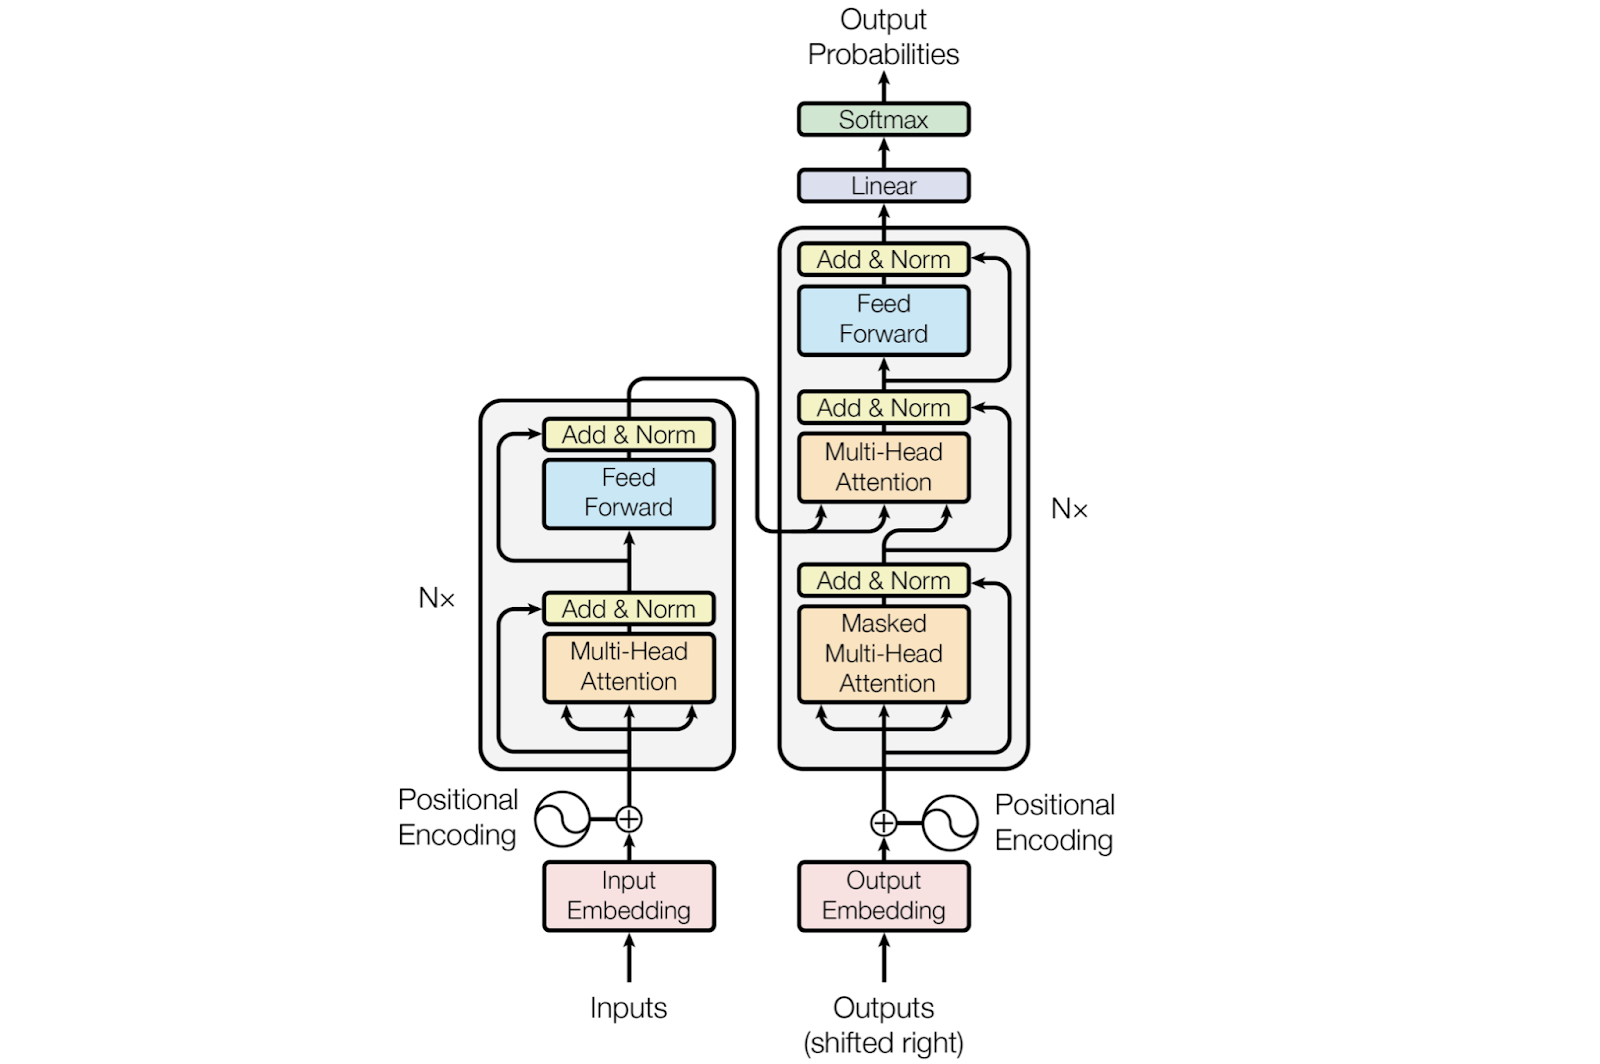
\includegraphics{image/transformers.png} Elle comprend trois
particularités

\begin{itemize}
\tightlist
\item
  le mécanisme d'attention ( Multihead attention)
\item
  l'encodage de la position des mots
\end{itemize}

\section{le mécanisme de
l'attention}\label{le-muxe9canisme-de-lattention}

C'est un article intitulé ``Attention is all you need'' de Vaswani et
al. (2017) qui est le germe d'une véritable révolution des modèles de
langage. IL propose une solution pour prendre en compte les relations
qui existent entre les différents termes d'un séquence de terme.

Cette solution est celle du mécanisme d'attention.

\section{Bert}\label{bert}

sur ce plan On doit beaucoup

\section{Les variations de bert}\label{les-variations-de-bert}

\subsection{le réentrainement}\label{le-ruxe9entrainement}

\subsection{Ajuster à des nouvelles
tâches}\label{ajuster-uxe0-des-nouvelles-tuxe2ches}

\section{Applications}\label{applications}

L'idée est d'entraîner un modèle de langue, sur de très larges corpus,
pour ensuite l'utiliser dans des tâches spécifiques.

\begin{figure}[H]

{\centering 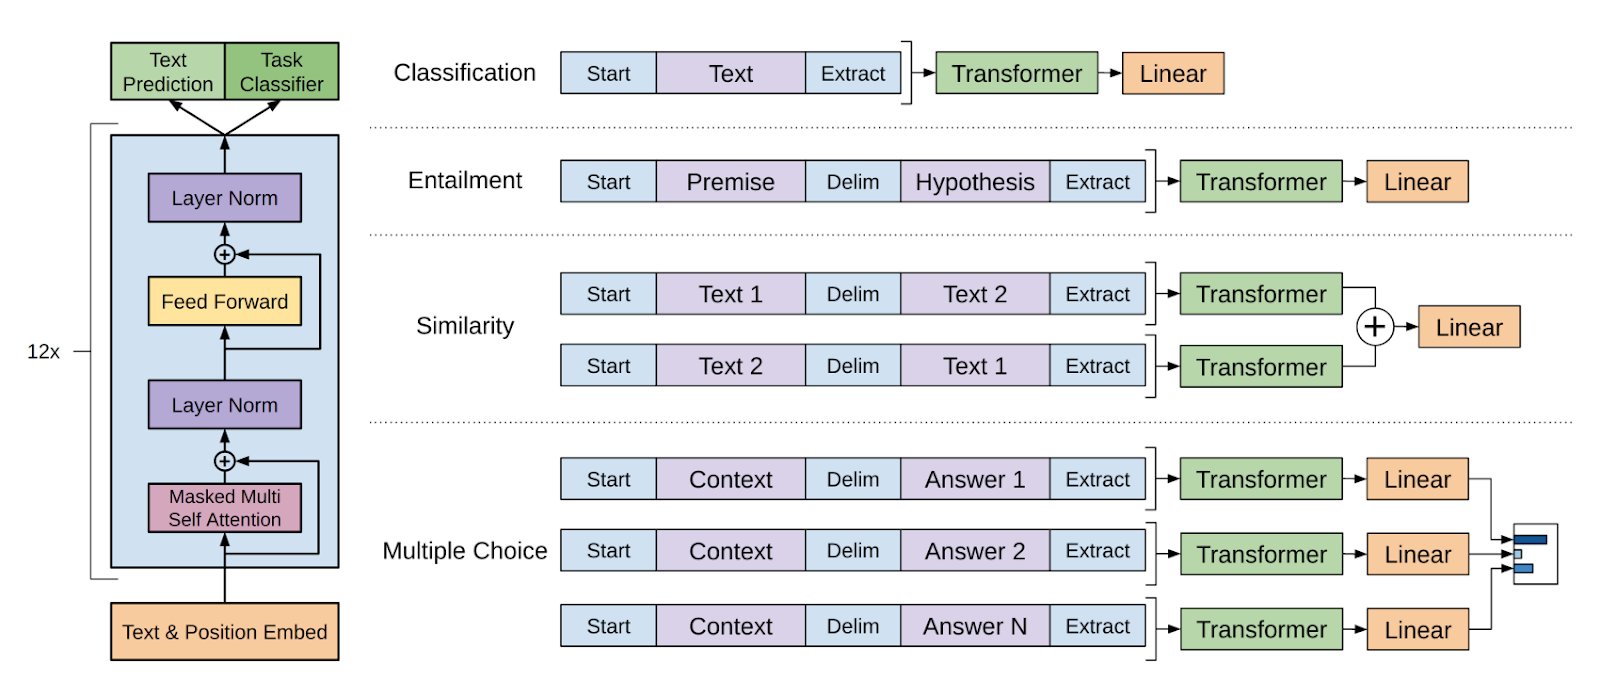
\includegraphics{multitaches.png}

}

\caption{Exemples}

\end{figure}%

Il ne s'agit pas ici de ré-entraîner des modèles, ce qui est une
approche tout à fait pertinente lorsque l'on est face à des corpus au
langage spécifique, mais d'utiliser les outils existants directement
disponibles.

Pour trouver le bon modèle à utiliser, il existe
\href{https://huggingface.co/}{Hugging Face}. La plupart des éléments de
code sont en python, mais il commence à exister des implémentations en
R.

Le problème véritable repose sur les temps de calcul et la puissance
disponible. On recommande d'avoir accès à un GPU, ce qui permet de
considérablement raccourcir le temps des traitements. Les outils en R
n'ont pas encore implémenté le recours au GPU, et nos ordis portables
n'en ont pas forcément. On peut avoir recours au cluster de calcul de
son université, ou utiliser les service de Google ou OpenAI (au prix
d'une facturation).

On va utiliser du code en python et du code en R pour analyser les
résultats. On travaille sur un tout petit corpus, pour limiter les temps
de calcul.

On pourra garder un oeil sur le package R
\href{https://www.r-text.org/index.html}{`text'} qui propose beaucoup
d'outils mais est encore en construction.

\subsection{Application de bert au
sentiment}\label{application-de-bert-au-sentiment}

\subsection{Application de bert au topic ( bert
model)}\label{application-de-bert-au-topic-bert-model}

Un classique du genre :
\href{https://maartengr.github.io/BERTopic/index.html}{BERTopic} de
Grootendorst (2022)

\begin{Shaded}
\begin{Highlighting}[]

\CommentTok{\#from bertopic import BERTopic}
\CommentTok{\#from bertopic.representation import KeyBERTInspired}

\CommentTok{\#import pandas as pd}

\CommentTok{\#df = r.data}
\CommentTok{\#print(df)}
\CommentTok{\#topic\_model = BERTopic(language="multilingual")}
\CommentTok{\#topics, probs = topic\_model.fit\_transform(df[\textquotesingle{}comments\textquotesingle{}])}
\CommentTok{\#topic\_model.get\_topic\_info()}
\CommentTok{\#topic\_model.get\_topic(8)}
\CommentTok{\#topic\_model.get\_topic\_freq().head()}
\CommentTok{\#topic\_model.get\_document\_info(df[\textquotesingle{}comments\textquotesingle{}])}
\CommentTok{\#topic\_model.find\_topics("réclamation")}
\CommentTok{\#topic\_model.generate\_topic\_labels()}

\CommentTok{\#topic\_model.visualize\_topics()}
\CommentTok{\#topic\_model.visualize\_heatmap()}
\end{Highlighting}
\end{Shaded}

\section{Références}\label{ruxe9fuxe9rences-3}

\bookmarksetup{startatroot}

\chapter{Classification with
embeddings}\label{classification-with-embeddings}

\textbf{Objectifs du chapitre :}

\emph{L'histoire de la linguistique computationnelle est intimement liée
au machine learning, et à la tâche de classification. Le principe
général de l'apprentissage artificiel consiste d'abord à choisir les
caractéristiques qui vont être employées pour prédire une variable
donnée, ensuite à choisir un modèle, puis à entraîner sur un premier jeu
de donnée, et enfin à l'évaluer sur la base d'un second échantillon de
données. Le processus est itératifs et vise à choisir les
hyper-paramètres les plus adéquation pour maximiser la capacité
prédictive du modèle}

\textbf{Environnement de travail}

\begin{Shaded}
\begin{Highlighting}[]
\CommentTok{\#les librairies du chapître}
\FunctionTok{library}\NormalTok{(tidyverse)}
\FunctionTok{library}\NormalTok{(tokenizers)}
\FunctionTok{library}\NormalTok{(quanteda)}
\FunctionTok{library}\NormalTok{(quanteda.textplots)}
\FunctionTok{library}\NormalTok{(flextable)}

\FunctionTok{theme\_set}\NormalTok{(}\FunctionTok{theme\_minimal}\NormalTok{()) }

\FunctionTok{set\_flextable\_defaults}\NormalTok{(}
  \AttributeTok{font.size =} \DecValTok{10}\NormalTok{, }\AttributeTok{theme\_fun =}\NormalTok{ theme\_vanilla,}
  \AttributeTok{padding =} \DecValTok{6}\NormalTok{,}
  \AttributeTok{background.color =} \StringTok{"\#EFEFEF"}\NormalTok{)}
\end{Highlighting}
\end{Shaded}

\section{Un cadre général}\label{un-cadre-guxe9nuxe9ral}

\begin{figure}[H]

{\centering 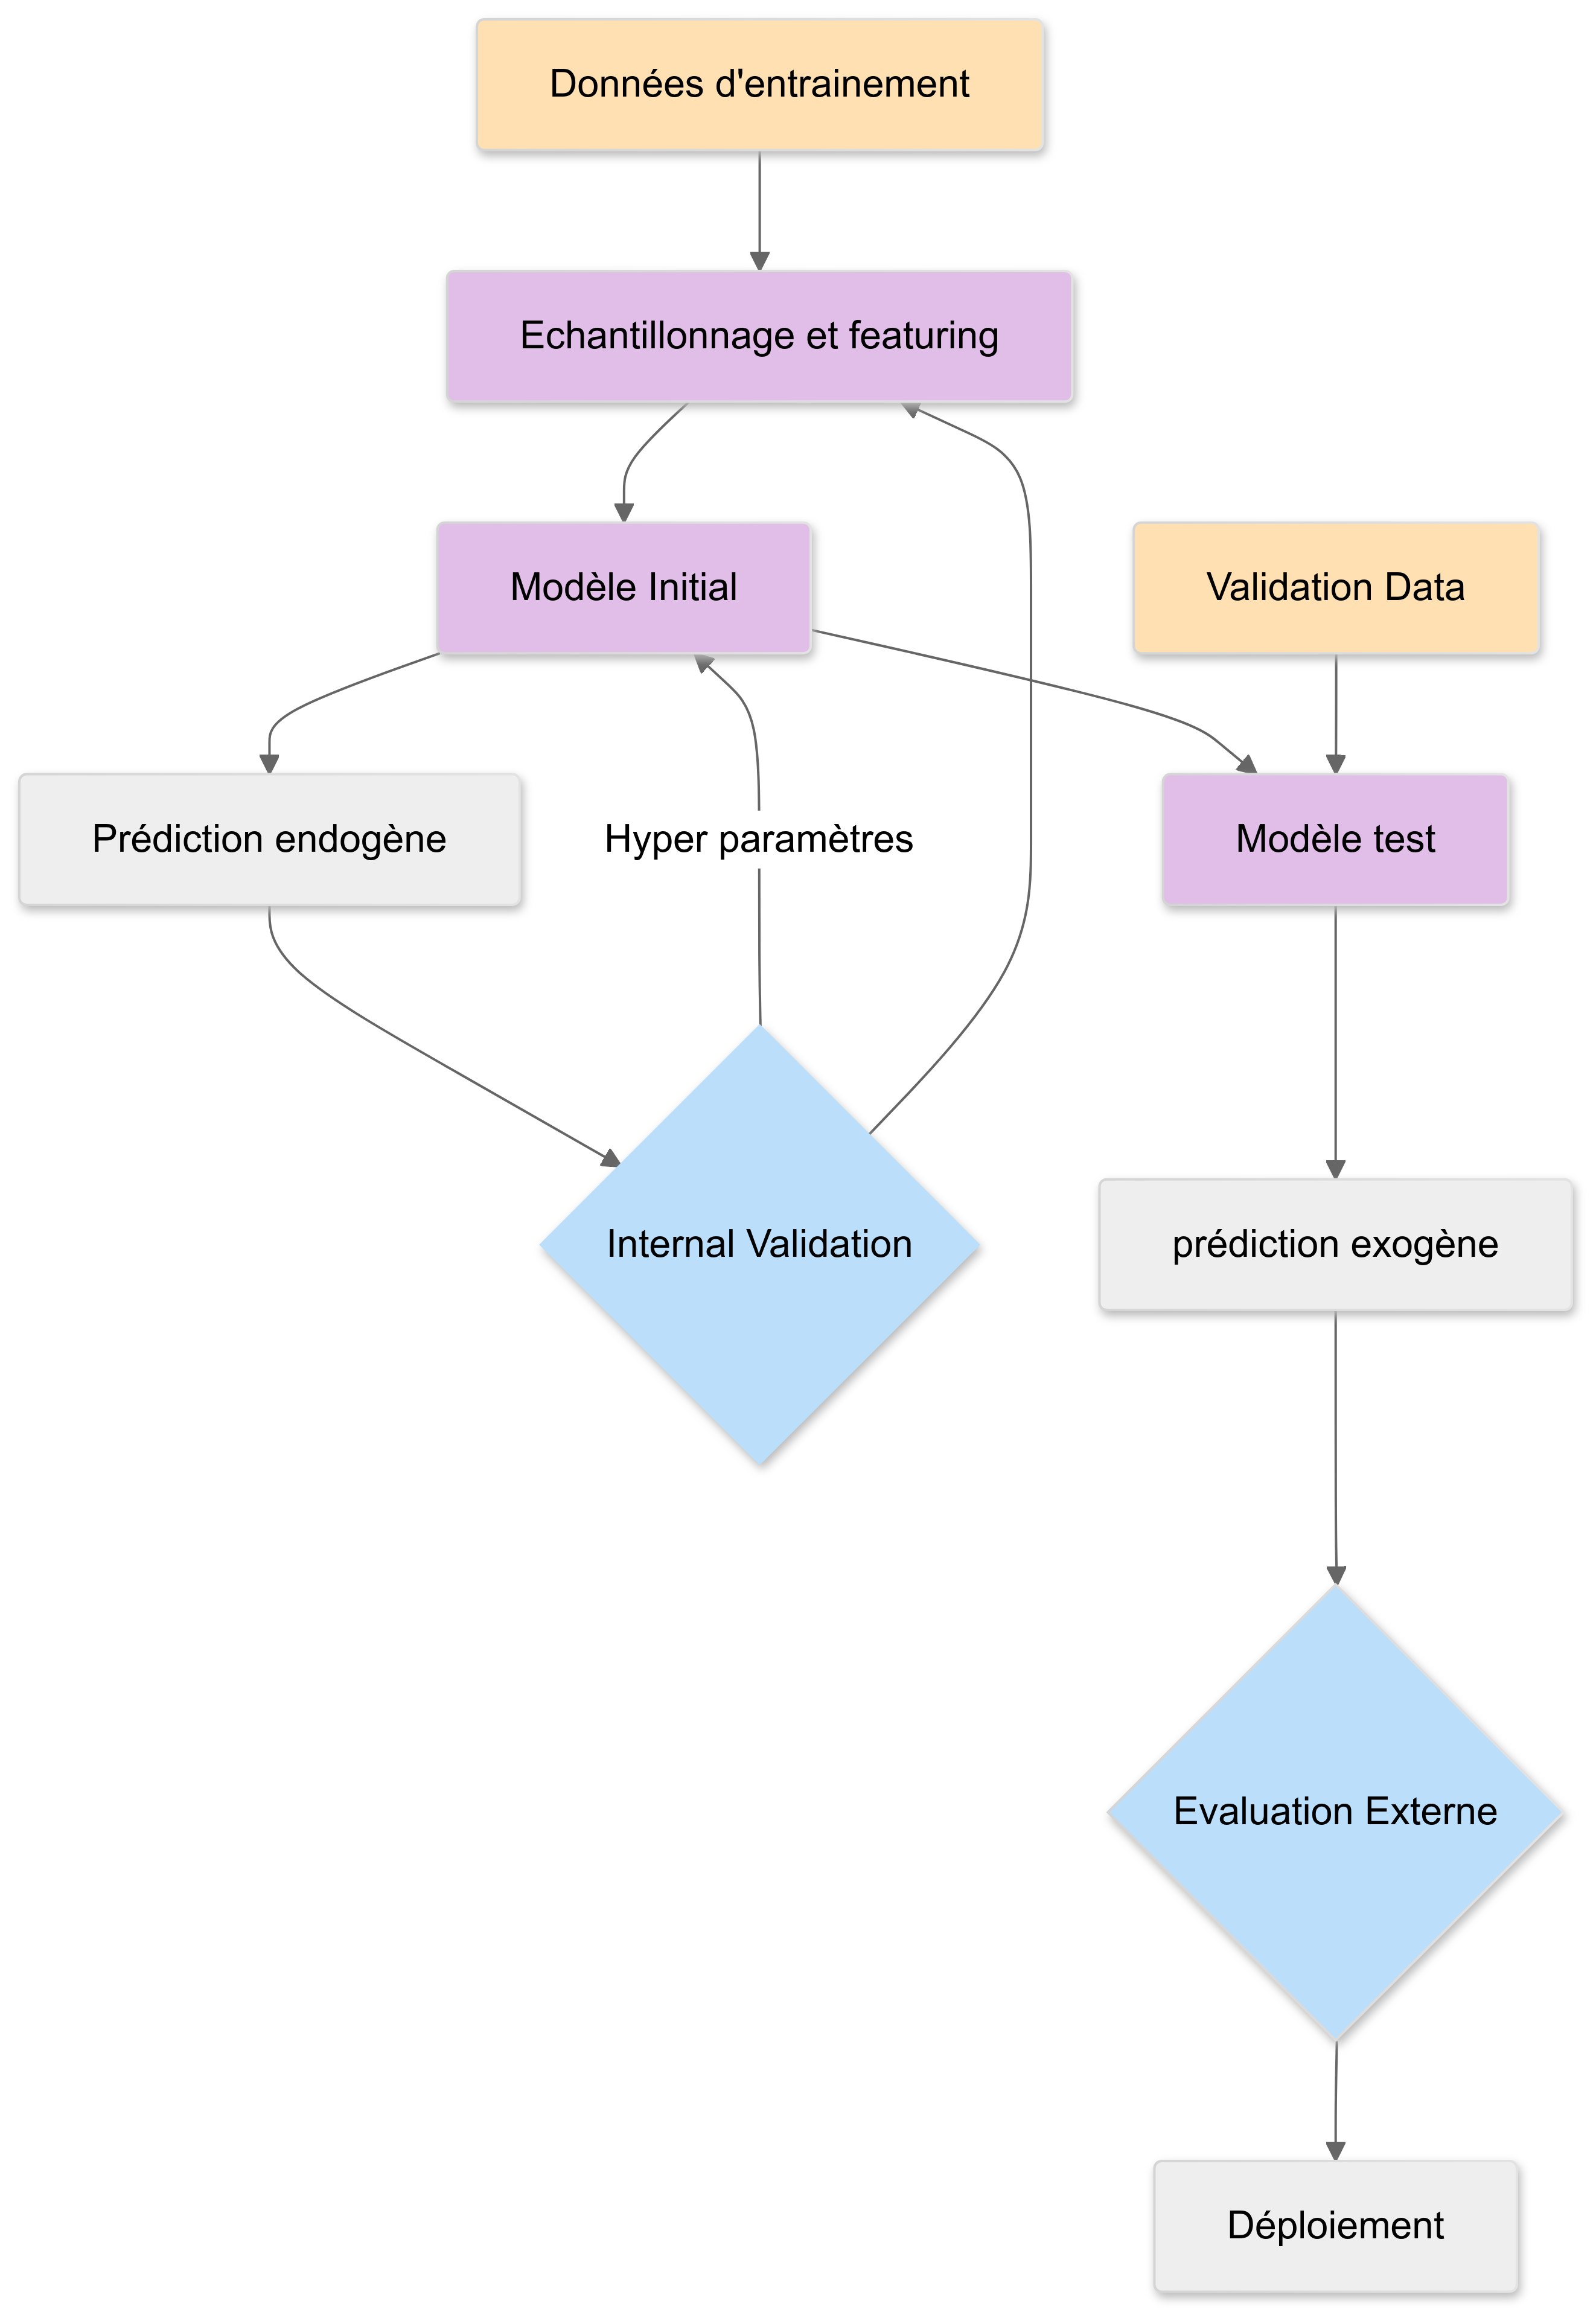
\includegraphics{image/ML2024.png}

}

\caption{Processus d'apprentissage machine}

\end{figure}%

-jouer avec les \href{https://playground.tensorflow.org/}{réseaux de
neurone} est forment recommandé.

\subsection{Ce qu'on cherche à
prédire}\label{ce-quon-cherche-uxe0-pruxe9dire}

le rôle central de l'annotation.

L'enjeu de l'annotation humaine. kappa.

\subsection{Avec quoi on cherche à
prédire}\label{avec-quoi-on-cherche-uxe0-pruxe9dire}

le featuring

les embeddings comme featuring, et un saut dans la performance

\subsection{Les modèles}\label{les-moduxe8les}

\begin{longtable}[]{@{}
  >{\raggedright\arraybackslash}p{(\columnwidth - 6\tabcolsep) * \real{0.1944}}
  >{\raggedright\arraybackslash}p{(\columnwidth - 6\tabcolsep) * \real{0.2778}}
  >{\raggedright\arraybackslash}p{(\columnwidth - 6\tabcolsep) * \real{0.2639}}
  >{\raggedright\arraybackslash}p{(\columnwidth - 6\tabcolsep) * \real{0.2639}}@{}}
\toprule\noalign{}
\begin{minipage}[b]{\linewidth}\raggedright
Col1
\end{minipage} & \begin{minipage}[b]{\linewidth}\raggedright
Continu
\end{minipage} & \begin{minipage}[b]{\linewidth}\raggedright
binaire
\end{minipage} & \begin{minipage}[b]{\linewidth}\raggedright
polytomique
\end{minipage} \\
\midrule\noalign{}
\endhead
\bottomrule\noalign{}
\endlastfoot
generation 1 & regression & Naive Bayes & \\
& Arbre de décision & & \\
génération 2 & lasso ( penalized) & Random forets & Random forest \\
génération 3 & réseaux neuronaux & réseaux neuronaux & réseaux
neuronaux \\
\end{longtable}

\subsection{Entrainement}\label{entrainement}

\subsection{Validation}\label{validation}

précision /rappel

roc

\subsection{Déploiement et
inférence}\label{duxe9ploiement-et-infuxe9rence}

\section{Un exemple simple : Naive bayes vs random
forest}\label{un-exemple-simple-naive-bayes-vs-random-forest}

Naive bayes :

Random forest :

\subsection{le processus}\label{le-processus}

\subsection{les résultats}\label{les-ruxe9sultats}

\section{Un exemple plus avancé : du Bert
sentiment}\label{un-exemple-plus-avancuxe9-du-bert-sentiment}

les modèles de langage fournissent un bon featuring

\subsection{le processus}\label{le-processus-1}

\subsection{les résultats}\label{les-ruxe9sultats-1}

\section{Conclusion}\label{conclusion-11}

Application à de nombreux concepts : - toxicité, ``profanité'',
complotisme - POS, - sentiment, émotions, personnalité \ldots{} -
detection d'élément thématiques - temporalité

Lourdeur de l'approche, incertitude du résultat : vers une approche plus
directe : le zeroshot classiqcation et le NER.

\bookmarksetup{startatroot}

\chapter{Introduction aux LLMs}\label{introduction-aux-llms}

\begin{Shaded}
\begin{Highlighting}[]
\CommentTok{\#les librairies du chapître}
\FunctionTok{library}\NormalTok{(tidyverse)}

\FunctionTok{theme\_set}\NormalTok{(}\FunctionTok{theme\_minimal}\NormalTok{()) }
\end{Highlighting}
\end{Shaded}

\textbf{Objectifs du chapitre :}

L'actualité du NLP est largement occupée par les performance
potentielles des IAG génératives qui s'appuient sur des représentations
du langage que contrôlent des modèles de renforcement fondés sur des
annotations humaines (RHLF). Cependant ils s'appuient sur un modèle
économique qui laisse peu de place à la transparence, et à la
persistance des modèles.

Pour les sciences sociales, les LLM ouverts présentent sans plus
d'intérêts, car plus pratiquables, et ré-entrainables pour s'ajuster à
des corpus spécifiques.

\section{La montée en puissance des
LLM}\label{la-montuxe9e-en-puissance-des-llm}

\emph{Bert} au départ. Plus de paramètres plus de données

\subsection{Modèles privés et modèles
ouvert}\label{moduxe8les-privuxe9s-et-moduxe8les-ouvert}

Le modèle privé est celui typique d'open AI, il s'impose par sa
puissance 3000 milliard de paramètres? La qualité de son apprentissage,
la généralité de son corpus, et se propose de résoudre l'ensemble des
problèmes de NLP .

les modèles ouverts, sont promus par les retardataires : meta avec
Llama, mistral, et rejouent les débuts de l'ère digitale. Ms-dos versus
linux. Le système ouvert n'est pas un modèle gratuit, c'est un modèle où
les acteurs s'accorde sur un standard public et construisent sur ce
socle des services spécifiques. Dans ce genre d'expérience, l'histoire
économique nous apprends qu'il y a deux équilibres et une polarisation
du marché.

\subsection{Une évolution
pré-cambrienne}\label{une-uxe9volution-pruxe9-cambrienne}

encoder et decoder

\href{https://github.com/Mooler0410/LLMsPracticalGuide}{source} (Yang et
al. 2023)

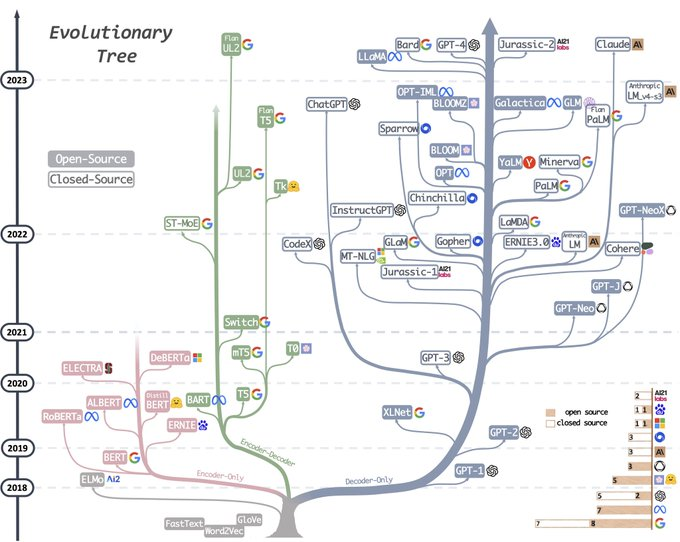
\includegraphics{image/LLMevolution.jpg}

\section{}\label{section}

Dans cette section on examine principalement l'usage des modèles ouverts
dans la veine de LLma, Mistral et les autres.

\section{Distributions}\label{distributions}

La première question posée par les modèles ouverts est celle de leur
exploitation qui requiert qu'ils puissent être opérables et que leurs
poids soient partagés. Hugging face est devenue le centre de gravité de
ce véritable écosystème. 14000 modèles déposés.

Leur opérationnalité est une question de hardware : taille de la
mémoire, usage de gpu, on comprendre que dans la logique de l'économie
de plateforme pour encourager l'usage de ces modèles, et peut être
imposer des standarts, les acteurs ont avantage à servir ces modèles en
différents rapport de taille et de performance, pour différents usages
ou capacités. Ils sont ainsi livré sous différentes version 7B, 13B, 70
MB, les premier pouvant être opérés sur une station de travail, les 70B
exigent un GPU. On constate l'effort d'offrir des tradeèoff.

L'enjeu est de réduire la taille des modèles, sans perdre excessivement
de précision.

\begin{itemize}
\item
  Certains modèles sont Distillés
\item
  Ils peuvent aussi être quantisisés. C'est l'idée d'arrondir les
  paramètre pour les rendre plus léger.
\end{itemize}

Ils peuvent être enfin entrainés à des fins particulières. Le NER ou le
SZC comme nous l'avons étudié auparavant.

\section{Ajuster les modèles à des tâches et des set de données
particuliers}\label{ajuster-les-moduxe8les-uxe0-des-tuxe2ches-et-des-set-de-donnuxe9es-particuliers}

En matière d'annotation, une première exigence est celle de la fiabilité
des mesures. Un modèle entrainé sur un corpus général est sans doute
moins performant qu'un modèle de plus petite taille qu'on réentrainé sur
un corpus spécifique.

C'est aujourd'hui la question principale à laquelle nous n'avons pas de
réponse définitive.

\subsection{Fine tuning}\label{fine-tuning}

Les LLMs sont entraînés sur des corpus vastes et hétérogènes, pour leur
donner plus de finnesse il peut être utile de les ré-entraîner sur des
corpus spécifiques. Mais comment faire?

pour entraîner un LMM, la tâche est simple : faire des trous dans le
texte et prédire le mot qui devait être dans le trous. ré-entraîner un
modèle général à un set de données particulier, reviens à trouer le set
de données, et à prédire les mots en modifiant les parametres du modèle
initial.

\subsection{Lora}\label{lora}

Le fine tuning est coûteux et des solutions sont rapidement apparu pour
réduit ce coût, l'approche lora en est un cas remarquable. L'idée est de
modifier qu'une partie des paramètres, plutôt les couches hautes.

Construire les data set d'apprentissage

\subsection{Rag}\label{rag}

DPO

\section{La question de la
validation}\label{la-question-de-la-validation}

\subsection{RHLF}\label{rhlf}

\subsection{post coorection}\label{post-coorection}

\subsection{measurement validity and
reliability}\label{measurement-validity-and-reliability}

\section{IAG}\label{iag}

\section{Conclusion}\label{conclusion-12}

\bookmarksetup{startatroot}

\chapter{Reconnaissance des entités nommées
(NER)}\label{reconnaissance-des-entituxe9s-nommuxe9es-ner}

\begin{Shaded}
\begin{Highlighting}[]
\CommentTok{\#les librairies du chapître}
\FunctionTok{library}\NormalTok{(tidyverse)}
\FunctionTok{library}\NormalTok{(tokenizers)}
\FunctionTok{library}\NormalTok{(quanteda)}
\FunctionTok{library}\NormalTok{(quanteda.textplots)}
\FunctionTok{library}\NormalTok{(flextable)}

\FunctionTok{theme\_set}\NormalTok{(}\FunctionTok{theme\_minimal}\NormalTok{()) }

\FunctionTok{set\_flextable\_defaults}\NormalTok{(}
  \AttributeTok{font.size =} \DecValTok{10}\NormalTok{, }\AttributeTok{theme\_fun =}\NormalTok{ theme\_vanilla,}
  \AttributeTok{padding =} \DecValTok{6}\NormalTok{,}
  \AttributeTok{background.color =} \StringTok{"\#EFEFEF"}\NormalTok{)}
\end{Highlighting}
\end{Shaded}

\textbf{Objectifs du chapitre :}

\emph{reconnaissance des entités nommées.}

\section{Le principe et l'histoire}\label{le-principe-et-lhistoire}

L'analyse des classes latentes

\section{Gliner}\label{gliner}

sur ce plan On doit beaucoup à sokal et sneath

\section{Application}\label{application-2}

\section{Conclusion}\label{conclusion-13}

\bookmarksetup{startatroot}

\chapter{Zero shot Classification}\label{zero-shot-classification}

\begin{Shaded}
\begin{Highlighting}[]
\CommentTok{\#les librairies du chapître}
\FunctionTok{library}\NormalTok{(tidyverse)}
\FunctionTok{library}\NormalTok{(tokenizers)}
\FunctionTok{library}\NormalTok{(quanteda)}
\FunctionTok{library}\NormalTok{(quanteda.textplots)}
\FunctionTok{library}\NormalTok{(flextable)}

\FunctionTok{theme\_set}\NormalTok{(}\FunctionTok{theme\_minimal}\NormalTok{()) }

\FunctionTok{set\_flextable\_defaults}\NormalTok{(}
  \AttributeTok{font.size =} \DecValTok{10}\NormalTok{, }\AttributeTok{theme\_fun =}\NormalTok{ theme\_vanilla,}
  \AttributeTok{padding =} \DecValTok{6}\NormalTok{,}
  \AttributeTok{background.color =} \StringTok{"\#EFEFEF"}\NormalTok{)}
\end{Highlighting}
\end{Shaded}

\textbf{Objectifs du chapitre :}

\emph{labelliser un corpus.}

C'est une application fondamentale pour les sciences sociales.

\section{le NLI}\label{le-nli}

L'analyse des classes latentes

\section{Une application avec}\label{une-application-avec}

sur ce plan On doit beaucoup à sokal et sneath

\section{generalisation}\label{generalisation}

\section{Conclusion}\label{conclusion-14}

\bookmarksetup{startatroot}

\chapter{Utilisation de l'IA
generative}\label{utilisation-de-lia-generative}

\begin{Shaded}
\begin{Highlighting}[]
\CommentTok{\#les librairies du chapitre}
\FunctionTok{library}\NormalTok{(tidyverse)}
\FunctionTok{library}\NormalTok{(tokenizers)}
\FunctionTok{library}\NormalTok{(quanteda)}
\FunctionTok{library}\NormalTok{(quanteda.textplots)}
\FunctionTok{library}\NormalTok{(flextable)}

\CommentTok{\# glossaire}
\FunctionTok{library}\NormalTok{(glossary)}
\FunctionTok{glossary\_path}\NormalTok{(}\StringTok{"glossary.yml"}\NormalTok{)}
\FunctionTok{glossary\_style}\NormalTok{(}\AttributeTok{color =} \StringTok{"purple"}\NormalTok{, }
               \AttributeTok{text\_decoration =} \StringTok{"underline"}\NormalTok{,}
               \AttributeTok{def\_bg =} \StringTok{"\#333"}\NormalTok{,}
               \AttributeTok{def\_color =} \StringTok{"white"}\NormalTok{)}
\end{Highlighting}
\end{Shaded}

\begin{Shaded}
\begin{Highlighting}[]
\FunctionTok{glossary\_popup}\NormalTok{(}\StringTok{"click"}\NormalTok{)}

\CommentTok{\#theme settings}

\FunctionTok{theme\_set}\NormalTok{(}\FunctionTok{theme\_minimal}\NormalTok{()) }

\FunctionTok{set\_flextable\_defaults}\NormalTok{(}
  \AttributeTok{font.size =} \DecValTok{10}\NormalTok{, }\AttributeTok{theme\_fun =}\NormalTok{ theme\_vanilla,}
  \AttributeTok{padding =} \DecValTok{6}\NormalTok{,}
  \AttributeTok{background.color =} \StringTok{"\#EFEFEF"}\NormalTok{)}
\end{Highlighting}
\end{Shaded}

\textbf{Objectifs du chapitre :}

\emph{IAG}

**

Généralité sur les l'IAG : (https://aiindex.stanford.edu/)

\begin{itemize}
\tightlist
\item
  la montée en puissance : une manière simple d'en rendre compte
\item
  le renforcement humain
\item
  Un nouvel art le prompt
\item
  Les applications
\end{itemize}

écarter l'usage génératif : création et résolution de problème.

\section{Prompter pour des tâches
classiques}\label{prompter-pour-des-tuxe2ches-classiques}

Pour le chercheur l'intérêt immédiat pour les VLLM est évidemment la
promesse de performance des annotations mais aussi leur flexibilité par
la procédure du prompt.

On présentera ici quelques exemples élémentaires

\subsection{NER}\label{ner}

\subsection{ZERO shot}\label{zero-shot}

\subsection{procédure générale}\label{procuxe9dure-guxe9nuxe9rale}

\begin{itemize}
\tightlist
\item
  utilisation de l'API
\item
  construire des boucles d'interrogations
\item
  valider les résultats
\end{itemize}

\section{L'élargissement du champs des
tâches}\label{luxe9largissement-du-champs-des-tuxe2ches}

Avec l'IAG le spectre des tâches s'élargit considérablement au delà de
l'annotation des éléments du texte ( ner et argumentation) et de
l'ensemble du texte ()

\subsection{Résumé}\label{ruxe9sumuxe9}

réduire le texte

structurer le texte.

l'apport des rag ( exemple coral AI)

\subsection{lecture d'image}\label{lecture-dimage}

Voici un essai de Image2Text réalisé avec Claude Sonnet 3.5 .

\emph{A : This image appears to be a vintage advertisement for DIM, a
French clothing brand known for hosiery and undergarments. The image
features a woman in a provocative pose, bending forward with her hands
touching the ground. She's wearing a shiny, metallic blue top, black
shorts or a short skirt, and black tights or stockings. Her hair is
short and blonde, styled in a somewhat messy or tousled manner. She
appears to be standing on a dry, cracked surface, possibly representing
a desert or dried lake bed. The text on the image reads: ``Merci à la
terre qui est si basse.'' (Thank you to the earth which is so low.)
``DIM'' ``Surtout en dim up.'' (Especially in dim up.) This text plays
on the woman's posture, bending low to the ground, and likely references
the brand's products, possibly suggesting they allow for flexibility or
movement. The ad seems to be using a combination of sexuality, wordplay,
and striking visuals to promote the DIM brand, which was common in
fashion advertising of certain eras. The overall aesthetic suggests this
may be from the 1980s or early 1990s.}

\begin{figure}[H]

{\centering 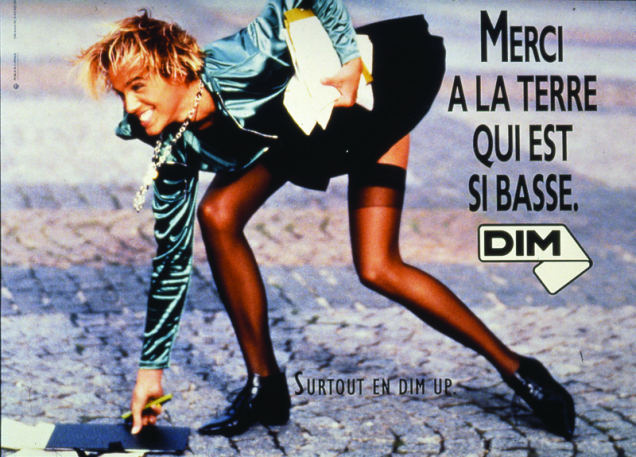
\includegraphics{image/pub_image_dim-4003100.jpeg}

}

\caption{exemple de la pub dim}

\end{figure}%

La première impression est plutôt très favorable, même si des omissions
et aveuglement peuvent être remarqués : le caractère provoquant vient de
ce que la pose fait entrevoir la peau de la cuisse au-dessous du bas.
C'est naturellement un poncif érotique, qu'atténue l'accident. Le
dernier paragraphe, en reprend l'idée mais sans en situer l'élément
visuel de manière précise. Quand à l'aveuglement, il s'agit du pavé que
la machine ne discerne pas, dérivant de la perception de surface (sèche
et craquelée) le lit d'une rivière asséchée. C'est ici un mirage au pied
de la lettre !

\section{Conclusion}\label{conclusion-15}

Un certain nombre de questions ouvertes quand à l'intérêt intrinsèque
des très grands modèles de langages:

\begin{itemize}
\tightlist
\item
  Un art ou une ingénierie du prompt.
\item
  la question de la réplicabilité.
\item
  La question de la vie privée et de la protection des données.
\item
  La question de la validation des mesures
\end{itemize}

\bookmarksetup{startatroot}

\chapter*{Glossaire}\label{glossaire}
\addcontentsline{toc}{chapter}{Glossaire}

\markboth{Glossaire}{Glossaire}

fonction glossaire

\begin{Shaded}
\begin{Highlighting}[]
\CommentTok{\# glossaire}
\FunctionTok{library}\NormalTok{(glossary)}
\FunctionTok{glossary\_path}\NormalTok{(}\StringTok{"glossary.yml"}\NormalTok{)}
\FunctionTok{glossary\_style}\NormalTok{(}\AttributeTok{color =} \StringTok{"purple"}\NormalTok{, }
               \AttributeTok{text\_decoration =} \StringTok{"underline"}\NormalTok{,}
               \AttributeTok{def\_bg =} \StringTok{"\#333"}\NormalTok{,}
               \AttributeTok{def\_color =} \StringTok{"white"}\NormalTok{)}
\end{Highlighting}
\end{Shaded}

\begin{Shaded}
\begin{Highlighting}[]
\FunctionTok{glossary\_popup}\NormalTok{(}\StringTok{"click"}\NormalTok{)}
\FunctionTok{glossary\_table}\NormalTok{()}
\end{Highlighting}
\end{Shaded}

tableau de données (data frame) avec 0 colonnes et 0 ligne

\bookmarksetup{startatroot}

\chapter*{References}\label{references}
\addcontentsline{toc}{chapter}{References}

\markboth{References}{References}

\phantomsection\label{refs}
\begin{CSLReferences}{1}{0}
\bibitem[\citeproctext]{ref-anastasopoulos_computational_2017}
Anastasopoulos, Lefteris Jason, Tima T. Moldogaziev, and Tyler Scott.
2017. {``Computational Text Analysis for Public Management Research.''}
\emph{{SSRN} Electronic Journal}.
\url{https://doi.org/10.2139/ssrn.3269520}.

\bibitem[\citeproctext]{ref-benzecri_analyse_2006}
Benzecri, Jean-Paul. 2006. {``L'analyse de Données : Histoire, Bilan,
Projets Et Perspectives,''} 5.

\bibitem[\citeproctext]{ref-blei_latent_2003}
Blei, David M., Andrew Y. Ng, and Michael I. Jordan. 2003. {``Latent
Dirichlet Allocation.''} \emph{J. Mach. Learn. Res.} 3 (March):
993--1022. \url{http://dl.acm.org/citation.cfm?id=944919.944937}.

\bibitem[\citeproctext]{ref-coleman_computer_1975}
Coleman, Meri, and T. L. Liau. 1975. {``A Computer Readability Formula
Designed for Machine Scoring.''} \emph{Journal of Applied Psychology} 60
(2): 283--84. \url{https://doi.org/10.1037/h0076540}.

\bibitem[\citeproctext]{ref-duval_analyse_2016}
Duval, Dominic, and François Pétry. 2016. {``L'analyse Automatisée Du
Ton Médiatique : Construction Et Utilisation de La Version Française Du
\emph{Lexicoder} Sentiment Dictionary.''} \emph{Canadian Journal of
Political Science} 49 (2): 197--220.
\url{https://doi.org/10.1017/S000842391600055X}.

\bibitem[\citeproctext]{ref-firth_synopsis_1957}
Firth, J. R. 1957. {``A Synopsis of Linguistic Theory 1930-55.''}
\emph{Studies in Linguistic Analysis (Special Volume of the Philological
Society)} 1952-59: 1--32.

\bibitem[\citeproctext]{ref-flesch_new_1948}
Flesch, Rudolph. 1948. {``A New Readability Yardstick.''} \emph{Journal
of Applied Psychology} 32 (3): 221--33.
\url{https://doi.org/10.1037/h0057532}.

\bibitem[\citeproctext]{ref-grootendorst_bertopic_2022}
Grootendorst, Maarten. 2022. {``{BERTopic}: Neural Topic Modeling with a
Class-Based {TF}-{IDF} Procedure.''} \emph{{arXiv} Preprint
{arXiv}:2203.05794}.

\bibitem[\citeproctext]{ref-humphreys_automated_2018}
Humphreys, Ashlee, and Rebecca Jen-Hui Wang. 2018. {``Automated Text
Analysis for Consumer Research.''} Edited by Eileen Fischer and Linda
Price. \emph{Journal of Consumer Research} 44 (6): 1274--1306.
\url{https://doi.org/10.1093/jcr/ucx104}.

\bibitem[\citeproctext]{ref-kobayashi_text_2018}
Kobayashi, Vladimer B., Stefan T. Mol, Hannah A. Berkers, Gábor
Kismihók, and Deanne N. Den Hartog. 2018. {``Text Mining in
Organizational Research.''} \emph{Organizational Research Methods} 21
(3): 733--65. \url{https://doi.org/10.1177/1094428117722619}.

\bibitem[\citeproctext]{ref-kozlowski_geometry_2019}
Kozlowski, Austin C., Matt Taddy, and James A. Evans. 2019. {``The
Geometry of Culture: Analyzing the Meanings of Class Through Word
Embeddings.''} \emph{American Sociological Review} 84 (5): 905--49.
\url{https://doi.org/10.1177/0003122419877135}.

\bibitem[\citeproctext]{ref-liu_sentiment_2012}
Liu, Bing. 2012. \emph{Sentiment Analysis and Opinion Mining}. Synthesis
Lectures on Human Language Technologies. Cham: Springer International
Publishing. \url{https://doi.org/10.1007/978-3-031-02145-9}.

\bibitem[\citeproctext]{ref-lock_quantitative_2015}
Lock, Irina, and Peter Seele. 2015. {``Quantitative Content Analysis as
a Method for Business Ethics Research.''} \emph{Business Ethics: A
European Review} 24 (July): S24--40.
\url{https://doi.org/10.1111/beer.12095}.

\bibitem[\citeproctext]{ref-tausczik_psychological_2010}
Tausczik, Yla R., and James W. Pennebaker. 2010. {``The Psychological
Meaning of Words: {LIWC} and Computerized Text Analysis Methods.''}
\emph{Journal of Language and Social Psychology} 29 (1): 24--54.
\url{https://doi.org/10.1177/0261927X09351676}.

\bibitem[\citeproctext]{ref-tweedie_how_1998}
Tweedie, Fiona J., and R. Harald Baayen. 1998. {``How Variable May a
Constant Be? Measures of Lexical Richness in Perspective.''}
\emph{Computers and the Humanities} 32: 323--52.

\bibitem[\citeproctext]{ref-vaswani_attention_2017}
Vaswani, Ashish, Noam Shazeer, Niki Parmar, Jakob Uszkoreit, Llion
Jones, Aidan N. Gomez, Lukasz Kaiser, and Illia Polosukhin. 2017.
{``Attention Is All You Need.''} {arXiv}.
\url{https://doi.org/10.48550/ARXIV.1706.03762}.

\bibitem[\citeproctext]{ref-verdelhan-bourgade_lucien_2020}
Verdelhan-Bourgade, M. 2020. {``Lucien Tesnière, Professeur de
Linguistique à Montpellier de 1937 à 1954. L'aventure d'une
Grammaire.''} \emph{Bulletin de l'Academie Des Sciences Et Lettres de
Montpellier} 51 (4562).

\bibitem[\citeproctext]{ref-yang_harnessing_2023}
Yang, Jingfeng, Hongye Jin, Ruixiang Tang, Xiaotian Han, Qizhang Feng,
Haoming Jiang, Bing Yin, and Xia Hu. 2023. {``Harnessing the Power of
{LLMs} in Practice: A Survey on {ChatGPT} and Beyond.''}

\end{CSLReferences}




\end{document}
